\documentclass{article}
\usepackage{tikz}
\usetikzlibrary{decorations.pathreplacing}
\usetikzlibrary{positioning}
\usepackage{hyperref}
\usepackage{apacite}
\usepackage{float}
\usepackage{geometry}
\usepackage{setspace}
\usepackage{adjustbox}
\usepackage{multirow}
\usepackage[T1]{fontenc} % for smaller printing smaller than sign correctly in plots
\usepackage[labelfont=bf]{caption} % for captions
\usepackage[toc]{appendix} % toc to show in table of contents
\usepackage{tabularx} % expanding tables
\usepackage{xltabular} % multipage tabularx
\usepackage{amsmath} % Align equations
\usepackage{booktabs} % toprule etc..
\usepackage{parskip}
\setstretch{1.5}
\geometry{left=20mm, right=50mm, top=20mm, bottom=10mm, includefoot}
\pagecolor{white}

\title{Cross-sectional predictability of stock returns in Nordic stock markets using machine learning methods}
\author{Jesse Keränen}
%add time period to all plot and tables once final

\begin{document}
\begin{titlepage}
\begin{center}
\vspace*{5em}
Master thesis submitted in partial fulfillment of the requirements for the degree\\
Master of Science \\
at Technische Universität München 

\vspace{7em}

\Large\textbf{Cross-sectional predictability of stock returns in Nordic stock markets using machine learning methods}

\vspace{7em}

\end{center}

\begin{tabular}{p{10em} l} 
\multirow[t]{4}{*}{Reviewer} 		& Prof. Dr. Christoph Kaserer\\ 
							& Department of Financial Management and Capital Markets\\ 
							& TUM School of Management\\ 
							& Technische Universität München\\[3ex]
Advisor: 						& Noorhan Elkhayat\\[3ex]
Study program: 				& TUM-BWL\\[3ex]
\multirow[t]{5}{*}{Composed by:} 	& Jesse Keränen\\
							& Motorstraße 64\\
							& 80809 Munich\\
							& Tel.: +49 (0) 1628410926\\
							& Matriculation number: 03748837\\[3ex]
Submitted on: 					& \today \\
\end{tabular}

\thispagestyle{empty}
\end{titlepage}

\newpage
\pagenumbering{Roman}

\tableofcontents

\newpage

\listoffigures
\listoftables

\newpage

\section{Introduction} \label{Introduction}
\pagenumbering{arabic}
In 1808 world was in many ways different compared to what it is today. In 1808 Napoleon was the Emperor of the French Empire and Maximilian I was the King of Kingdom of Bavaria. In 1808 Finnish war broke between Kingdom of Sweden and the Russian Empire which would ultimately lead to establishment of autonomous Grand Duchy of Finland. It would still take more than 100 years for Finland to gain its independence. Same year began the Dano-Swedish war between Sweden and Denmark-Norway. Something historically far less remarkable, but essential for this study happened in 1808 as well. First stock exchange in a Nordic country was opened in Copenhagen. Slowly after that rest of the Nordic countries would open their own stock exchanges as well. Upon facilitated change of ownership of assets, investors were left with a question how to price these assets. \par

Major breakthrough in this topic happened when capital asset pricing model was developed in the sixties (sharpe, treynor etc...). In the eighties persofrmance of capital asset pricing model was questioned and scholars came up with so called stock market factors (Earnings-to-price = Basu(1977), Earnings-to-price = Basu(1977), Profitability = e.g., Basu, 1983). During these time machine learning gained large interest and artificial neural networks were popularized. Next big step in asset pricing happened when Eugene Fama and Kenneth French combined these factors to three factor asset pricing model (fama french 1993). Two years after that machine learning method called random forest was introduced (Ho in 1995). Although three factor model was remarkable improvement compared to capital asset pricing model it was not able to explain variation in stock returns completely. In recent years lot of research has applied machine learning methods to capture abnormal returns in stock markets. \par

%Nordic market introduction
Objective of this study is to apply set of machine learning methods to well established asset pricing factors to capture abnormal stock return patterns. This study will focus on four Nordic stock markets namely Denmark, Finland, Norway and Sweden. These four markets are relatively homogenous in many aspects. They are geographically close, politically stable and economically interconnected. Denmark, Finland and Sweden all belong to European union. Additionally, stock exchanges of all these three countries are operated by Nasdaq. Therefore, investors could view them as a single market. Some of the features that are characteristic for Nordic markets make them fertile ground for stock market anomaly studies. As mentioned Nordic countries are geographically closely located in northern Europe and therefore relatively distant from large European and especially American markets. European market integration is emphazised also by Fama and French \citeyear{FAMA2012457}. \par

So called periphery effect has been studied by the scholars a lot. %references)
It refers to investor behaviour where during times of a crisis investors tend to liquidate their investments first from the markets more distant to them. This increases the volatility of periphery markets and can challenge the efficient market theory. Another common feature that Nordic markets share is a high level of foreign ownership. Share of foreign investments in Nordic stock markets can reach more than 50\% \footnotemark. Given the remote location of Nordic stock markets and their high share of foreign ownership it is likely that Nordic countries could be subject to periphery effect. Which again can result abnormal returns. \par

This study contributes to the existing literature in several ways. First of all it applies machine learning framework from Gu, Kelly and Xiu \citeyear{guetal} to new market. Machine learning approach has been applied to European markets, but this study focuses on arguably even more coherent nordic submarket \cite{Drobetz, Fieberg}. Objective is to examine if investor investing only in Nordic markets could benefit from implementing the machine learning framework of Gu et al. \citeyear{guetal}. Dataset of study is unique in a sense that lot of machine learning approach studied have been conducted in more wider markets such as European stock markets, where as Nordic stock market anomaly studies mainly focuses on single markets. Pooling the four Nordic markets ensures us sufficient amount of data to train complex machine learning model, but also allows us to focus on homogenous clearly defined submarket. \par

Additionally, existing stock market anomaly literature focusing solely to Nordic markets is rather limited. Section \ref{NordicStockMarketAnomalies} introduces the existing stock market anomaly literature. Characteristic for studies in this section is that they mainly focus on one to two stock market anomalies. As this constructs 23 stock characteristic anomalies, it allows us examine anomalies that have not been applied to Nordic markets previously. Meaning that this study can not only reveal the profitability of machine learning framework in Nordic market setting, but it can also reveal existence of certain stock market anomalies in Nordic markets. As mentioned lot of Nordic stock market anomaly research focuses only up to two anomalies at once. Since this study includes 23 anomalies simultaneously, it allows us also to examine performance of already discovered Nordic anomalies while controlling for many other variables. Applying sophisticated machine learning models allows us to also to control for complex interactions. \par

Objective of this study is slightly more ambitious than in existing Nordic stock market anomaly literature. Existing literature mainly examines existence of anomalies by uni- or multivariate portfolio sorts. Studies predefine variable of interest and form portfolios based on that variable. Then the historical excess returns are investigated. This study goes one step further and attempts to predict stock level out-of-sample returns based on the predefined set of variables. This allows us to evaluate which portion of the return variability these variables are able to capture in addition to the profitability of the strategy. \par

Final contribution of this study is to expand the explanatory variable set. This study includes variable called on-balance volume. On-balance volume is a technical trading indicator which has not been studied in great extend as cross-sectional stock return predictor. Due to strong performance of momentum indicators, this study includes several momentum indicators. Extended variable set allows us to examine whether on-balance anomaly exists in Nordic stock markets or whether including on-balance volume affects performance of well established momentum indicators. \par

%all developed, but small -> liquidity

Structure of this paper goes as follows. In second chapter introduction to related literature is provided. In this chapter performance of different methods and persistence of different anomalies in different regions is discussed. Third chapter introduces the data used in this study and filters applied to the data. Fourth chapter presents the methodology. It introduces the implemented models in more detail and describes the measurements applied for the models. Fifth chapter describes the results of the empirical study. Fifth chapter is divided to discuss separately predictive accuracy, economic profitability and covariate importance for the machine learning models.Finally the last chapter provides conclusion of the empirical study. \par

\footnotetext{Butt and Hogholm \citeyear{ButtHogholm2020} calculate share of foreign ownership from IMF Coordinated Direct Investment Survey CDIS data. Foreign ownership share of Butt and Hogholm is 52\% for Denmark, 42\% for Finland, 35\% for Norway and 56\% for Sweden. %check the source
}

\section{Literature}\label{Literature}
Being the largest and most prominent stock market in the world US stock market has been subject to majority of asset pricing studies. Despite the dominance of US markets in capturing the the attraction of the academics lot of anomaly asset pricing literature has been conducted in international setting as well. Characteristic for international asset pricing literature is that instead of focusing on single countries they aggregate stock market data to a certain regional level such as Europe or Asia-Pacific. Following chapter provides an overview for pioneering asset pricing anomaly literature. Focus will mainly be on literature on US and European markets. US stock markets are chosen because of their significant impact on international stock markets and because most anomalies have been discovered there and therefore majority of the initial studies of these anomalies have been conducted there. European studies provide interesting perspective for this study since in many of them Nordic countries are included. \par

Chapter introduces the most important anomalies in these markets and how they have been exploited with different methods. This works as starting point to define set of factors that will be used in this study. It can be argued that this kind of process when the set of variables are chosen based on their performance in previous studies is one sort of forward looking information if we try to mimic investors information set. On the other hand Jacobs and Müller \citeyear{JACOBS2020213} only find reliable post-publication decline in long/short returns in US which emphasizes the practical potential of this study. \par

\subsection{US stock market anomalies}\label{USStockMarketAnomalies}

Many of the recent cross-sectional stock return studies use framework of Lewellen \citeyear{Lewellen2015} as base model. He runs 10-year rolling Fama-MacBeth regressions using lagged firm characteristics to predict out of the sample stock returns. He studies cross-sections of US stock return between 1964 and 2013 using different model settings up to 15 company characteristics. He finds strong positive correlation between expected return derived from rolling Fama-MacBeth regressions and realised returns. Additionally Lewellen shows that spread between realised return of portfolio formed from stock with lowest expected returns and portfolio with highest expected return is up to 2.36\%. In his study logarithmic market value of equity, logarithmic book-to-market value, momentum and accruals show the strongest statistical power in explaining monthly returns using lagged variables. \par

Gu, Jelly and Xiu \citeyear{guetal} contribute to the literature by applying machine learning methods to exploit stock market anomalies. By deploying sophisticated models that do not suffer from over parameterization as heavily as OLS Gu et al. are able to include 94 stock characteristics and their interactions as well as eight aggregated time series variables to their models. Gu et al. use large variety of statistical methods including linear regression, generalized linear models with penalization, dimension reduction via principal components regression and partial least squares, gradient boosted regression trees, random forest and different settings of neural networks. Out of these gradient boosted regression trees and neural networks \footnotemark explain the monthly out of sample stock return the best reaching out of sample $R^{2}$ 0.33 and 0.44 correspondingly where as three factor OLS model introduced by Lewellen \citeyear{Lewellen2015} only reaches out of sample $R^{2}$ of -3.46. \par

\footnotetext{Gu et al. \citeyear{guetal} use five different settings of neural networks differing by number of hidden layers. Neural network with three hidden layers reaches the highest $R^{2}_{oos}$ and is reported here.}

Similar to Lewellen \citeyear{Lewellen2015} Gu et al. construct portfolios based on predicted return of different models. Monthly spread in realized return between portfolio constructed from decile of companies with lowest expected return and decile of stocks with highest expected return \footnotemark is 0.94, 1.62 and 2.12 for models based on OLS, random forest and three layer neural network correspondingly. Gu et al. also show that all methods they examine show somewhat similar patterns on variable importance on return predictability. Most important factors are price trends such as momentum followed by stock liquidity, stock volatility, and valuation ratios. \par
% all stocks, confirm again
% Deeper neural networks seem to be too complex

\footnotetext{Portfolio returns are average value weighted returns.}

\subsection{European stock market anomalies}\label{EuropeanStockMarketAnomalies}

As mentioned US market environment is different in my ways compared to Nordic markets. Fortunately lot of stock market studies have been conducted in Europe and since Nordic markets are usually just a subset of European markets it can be beneficial to have a look on European studies. Tobek and Hronec \citeyear{TOBEK2021100588} study machine learning based anomaly strategies in international setting. Their study includes 153 different equity anomalies and they only include anomalies to their data after documented discovery of corresponding anomaly. This way they can mimic the information set investor would have had and avoid forward looking information. Tobek and Hronec examine five different models including weighted least squares, penalized weighted least squares, gradient boosting regression trees, random forest and neural networks. Their data set spans from 1990 to 2018. \par

Similar to Gu et al. \citeyear{guetal} in US, Tobek and Hronec find that strategy using neural networks provides highest returns on quintile long-short portfolios. Mean return for neural network long-short portfolio in Europe was 0.7. Interestingly penalized weighted least square method provided mean return of 0.651 which is higher than return of random forest based portfolio's return of 0.396. Tobek and Hronec find that Industry momentum, lagged momentum, liquidity shocks, 52 week high, book-to-market value and return on equity are the most important variables for neural networks model.\footnotemark \par

\footnotetext{Tobek and Hronec \citeyear{TOBEK2021100588} discover possibilities training models either only using historical data from US, using historical data from local markets or using international historical data. Only results for models trained using local data are reported here because that is closest to the setting of this study. Additionally, Tobek and Hronec state that difference between model trained on US data and local data are small.}

Exploiting stock market anomalies using machine learning methods is also studied by Drobetz and Otto \citeyear{Drobetz}. Their data set contains all companies listed in at least one of the 19 Eurozone countries on December 2020 and spans form 1990 to 2020 \footnotemark. Drobetz and Otto examine performance of ordinary least squares, penalized least squares, principal components regressions, partial least squares, random forests, gradient boosted regression trees and neural networks on predicting monthly stock level return exploiting a set of 22 predictions, their two-way interactions and second- and third-order polynomials. Findings of Drobetz and Otto are similar to Gu et al. \citeyear{guetal}. They show that with large number of explanatory variables simple linear regression is not able to explain out of the sample stock returns. \par

\footnotetext{Finland is the only country included in the study of Drobetz and Otto \citeyear{Drobetz} that is also included in this study, since it is the only country belonging to Eurozone.}

Findings of Drobetz and Otto \citeyear{Drobetz} are also similar to Tobek and Hronec \citeyear{TOBEK2021100588} in a sense that least squares methods where dimensionality is restricted can actually perform better than tree based methods. Like in majority of other literature, Drobetz and Otto find out that neural networks provide superior framework for stock return prediction model measured in both explanatory power and profitability. Neural network method reaches out of the sample $R^{2}$ value of 1.23 and long-short portfolio formed based on expected returns derived from neural networks model provide average value weighted monthly return of 1.94\%. Similar to Gu et al. \citeyear{guetal} Drobetz and Otto find that same variables show the most importance across the different models, most notably earnings-to-price ratio and 12 month momentum. \par
%Deeper neural networks seem to be too complex

Fieberg et al \citeyear{Fieberg} study stock market anomalies in 16 European stock markets using machine learning methods over almost the same period as Drobetz and Otto \citeyear{Drobetz} \footnotemark. Nevertheless they choose a slightly different approach where instead of including vast set of anomalies, they only consider six prominent equity factors. Their conclusion endorses findings of Drobetz and Otto \citeyear{Drobetz} and Tobek and Hronec \citeyear{TOBEK2021100588} as they shown that more complex machine learning models beat linear approach in terms of both economic and statistical performance. \par

\footnotetext{Dataset of Fieberg et al \citeyear{Fieberg} contains Denmark, Finland, Norway and Sweden.}

\subsection{Nordic stock market anomalies}\label{NordicStockMarketAnomalies}

This chapter provides an overview of observed stock market anomalies in different Nordic stock markets. Many studies in this chapter have slightly different objective than this study. Studies show the existence of the anomalies by constructing a portfolio heavily weighted on certain factor. Nevertheless, they do not describe the magnitude of the relationship between the factor and the stock returns. This study has slightly more ambitious objective and tries to derive return expectations from predefined stock market factors. This literature review serves as starting point for choosing most promising stock market factors that have already been studied. \par
%small amount of stocks

Magnitude of value and momentum anomalies in Nordic stock markets are examined in the paper by Grobys and Huhta-Halkola \citeyear{grobys}. They combine information from companies listed in main lists of Danish, Finnish, Norwegian and Swedish stock exchanges between 1991 and 2017. Grobys and Huhta-Halkola measure value with book-to-market value and momentum with past 12-month total shareholder equity%return??? % 
. Grobys and Huhta-Halkola show that momentum effect exists in Nordics markets and profitability of momentum strategy is not related to size factor. Value factor yields also significant excess return, but according to Grobys and Huhta-Halkola it could be partly driven by the size factor, since value premium reduces when accounted for the size. Among all stocks monthly average equally weighted long-short return is 1.73\% and 1.25\% for momentum and value strategies correspondingly. Both of the excess returns are statistically highly significant. Grobys and Huhta-Halkola also test combination strategies using signals from both momentum and strategy which yield even stronger results. \par

Value premium has shown consistency in Finnish stock markets. Davydov, Tikkanen and Äijö \citeyear{Davydov2017MagicFV} examine profitability of different value investing strategies between 1991 and 2013. Davydov et. al. investigate set of value indicators which included earnings to price, book to price, cash flow to price, dividends to price and earnings before income and taxes to enterprise value ratios. Additionally they test performance of investing strategy developed by Greenblatt (cite here) where portfolios are formed based on combined ranking of company's return on invested capital and earnings before income and taxes to enterprise value ratio. They show that returns of all of the value portfolios not only beat the market return, but can also not be explained by the four factor model of Carhart \citeyear{https://doi.org/10.1111/j.1540-6261.1997.tb03808.x}.  \par
%(Finnish Stock Exchange in the period 1991–2013. In total, the number of companies varies from 39 to 136)
%check the second article from patari and leivo

Similar to Grobys and Huhta-Halkola \citeyear{grobys} Leivo and Pätäri \citeyear{leivo2011} combine value anomaly with momentum anomaly in Finnish stock market for data set between 1993 and 2008. They show that two step portfolio sort that first allocates stocks to three portfolios based on their value indicators and subsequently based on momentum indicator can capture extraordinary stock returns. Leivo and Pätäri show that including momentum further increases returns of already recognised value sorting. Strategy performs even better when authors allow for long position in high value high momentum portfolio and short position on low value low momentum portfolio. Excess returns resulting from the two-fold portfolio construction can not be explained by CAP-model or two factor model including also size factor. It is not a surprise that value and momentum premium show existence in Nordic markets. Value and momentum anomalies are among the most well documented factors showing persistence in multiple cross-sectional studies (e.g, Gu, Jelly and Xiu \citeyear{guetal}, Lewellen \citeyear{Lewellen2015}, Drobetz and Otto \citeyear{Drobetz}, Tobek and Hronec \citeyear{TOBEK2021100588}). \par
% Helsinki Stock Exchange (HEX; later OMX Helsinki) during the period 1993–2008. E/P, EBITDA/EV, CF/P, dividend yield (D/P), B/P and S/P and combinations.
%re-phrase the text

Nordic stock markets have several characteristic features. One is that all Nordic stock markets are considered to be developed, but also small. Especially market capitalization of companies listed in Nordic stock exchanges are on average much smaller than in US. Therefore, it is reasonable to ask whether liquidity of the stock could be driving factor of the stock returns. Impact of illiquidity risk to stock returns in Nordic market setting has been studied by Butt and Hogholm \citeyear{ButtHogholm2020}. Butt and Hogholm test variety of different illiquidity measures and find that dollar zero returns is the most profitable illiquidity anomaly measure across all four Nordic market. Dollar zero return measurement is calculated by dividing number of days stocks return in US dollars is zero by total number of trading days. Butt and Hogholm construct five quintile portfolios based on liquidity of the stocks with data spanning from 1988 to 2013. They show that in all Nordic markets there exists large illiquidity premium as annual difference in equal weighted return of most illiquid portfolio and least illiquid portfolio is more than 18\% for Finland, Norway and Sweden. For Denmark premium is slightly smaller 8.8\%. \par

Jokipii and Vähämaa \citeyear{jokipii2006free} investigate free cash flow anomaly in Finnish stock markets between 1992 and 2002. They construct portfolios from stocks listed in Finnish stock exchange based on predefined thresholds for free cash flow ratios. These ratios include market value to free cashflow and total debt to free cashflow ratios. High free cashflow portfolio yields higher returns than market on average and the excess returns can not be completely explained by weightings in Fama and French \citeyear{FAMA19933} risk factors. \par
%Finnish companies during the period 1992-2002. net cash flow from operating activities minus capital expenditures. The net cash flow from operating activities, in turn, is defined as the sum of net income, all non-cash charges and credits (e.g.,  depreciation,  amortization  of  intangibles,  and  deferred  taxes),  extra ordinary items, and net change in working capital

\section{Data}\label{Data}

This section provides an overview of the dataset used in this study. Section starts by introducing overall market setting in Nordic stock markets. Section discusses how companies are distributed across Nordic markets and also describes the size properties of the companies in different Nordic markets. This part also describes the static and dynamic screens applied to the Datastream data in order to ensure sufficient data quality. Second part of the section describes the firm level characteristics considered in this study. This stock level excess returns as well as all independent variables. This part introduces definitions of all variables including which characteristics are included calculation of each variable. Descriptive statistics of the firm level characteristics are also presented in this part of the study. \par

\subsection{Nordic stock market data}\label{NordicStockMarketData}

Main datasource for this study is Thomson Datastream. Company fundamentals data is collected from Worldscope database. Dataset spans from 1990 January to 2022 December which is shorter than in many previous studies. Reason why time period is limited to 1990 is that the amount of publicly listed companies in Nordic markets was rather low in the 1980's and finding reliable data for period before 1990 is difficult. Dataset contains all stocks listed in primary markets of corresponding countries including also companies that went bankrupt or were de-listed for any other reason. Therefore, dataset is not subject to survivorship bias. \par

Panel A of table \ref{table:constituteLists} in Appendix shows the constituent lists used in data collection. As highlighted by Ince and Porter \citeyear{Ince2006} data in Datastream can be noisy and uncleaned data could lead to a false statistical inference. Therefore, several static and dynamic screens are applied to the data. Static screens include filtering non-equity securities, securities that are not listed in respective country and securities that are quoted in currency other than respective country's currency. Panel A from table \ref{table:StaticScreens} shows which values are accepted for type of instrument, ISIN code, code indicating the country of origin of the company, country where the security is listed, currency in which the security is noted and ISIN country code. \par

In order to filter non-common and duplicate stock affiliations. Keywords indicating non-common stock affiliations are searched from Datastream attributes NAME, ENAME and ECNAME. Panel B of table \ref{table:StaticScreens} presents the country specific keywords. These keywords are only considered searched for securities from specific countries, but among all above mentioned attributes. Keywords from table \ref{table:GeneralKeywords} are searched from name attributes of securities from all countries. If a keyword is found from any of the name attributes, the security will be removed from the dataset. Keyword deletion follows Ince and Porter \citeyear{Ince2006} and Hanauer and Windmüller \citeyear{HANAUER2023106712}. \par

Ince and Porter \citeyear{Ince2006} argue that data quality issues in Datastream could even lead to wrong conclusions. In order to avoid results to be driven by extraordinary datapoints, which could be caused by data quality issues, dynamic screens are applied to the data. Table  \ref{table:DynamicScreens} in the appendix presents the applied dynamic screens. Observations are removed from the dataset in case of extreme abnormal return. Observations are also removed in case of extremely strong strong return reversals.\par

One characteristic has to be taken into consideration when working with data from Datastream. In case company is delisted for some reason Datastream returns last available value for remaining periods in the query. In order to only include actively traded securities these observations have to be cleaned from the dataset. This could be done with variable TIME from Datastream which shows the date of last equity price data. Nevertheless, Ince and Porter \citeyear{Ince2006} argue that the TIME attribute is not reliable indicator of the delisting date, but propose to remove consecutive zero returns from the end of the dataset. Removal of zero returns at the end of the dataset could lead to removal of actual zero returns, but the effect of this is considered to be smaller than the noise caused by the usage of TIME variable. Therefore, all consecutive zero returns at the end of the dataset are removed for all companies. \par

\begin{table}[h] 
\small
\caption[Country summary statistics]{\textbf{Country summary statistics}\\ Table provides summary statistics for pooled Nordic market and separate country specific Nordic markets. Minimum number of companies tells the amount of companies included to the data set in a month that the value was lowest for respective country. Maximum number of companies tells the amount of companies included to the data set in a month that the value was highest for respective country. Mean number of companies is the time series average of monthly number of companies for each country. Total number of companies is the number of unique companies in whole data set. Time series averages for monthly mean, median and total market values are also presented. Total market value is the sum of market values of respective country in each month. All marked values are converted to USD. Only companies in the final dataset are included in calculation of the figures. Micro stocks are excluded from the dataset.}
 \label{table:CountrySummary}
\centering
\newcolumntype{Y}{>{\centering\arraybackslash}X}
\begin{tabularx}{\textwidth}{@{\extracolsep{4pt}} X Y Y Y Y Y Y Y} 
\toprule
 & \multicolumn{4}{c}{Number of companies} & \multicolumn{3}{c}{Market value} \\
\cline{2-5} \cline{6-8} 
Market		& Min 	& Max 	& Mean  	& Total	& Mean 		& Median 	& Total \\
\midrule
Denmark	 	& 42		& 106 	& 70	 	& 235	& 2399.78 	& 810.32	& 141657.9  \\
Finland	 	& 26 		& 83	 	& 62		& 186 	& 1893.43 	& 634.47	& 124389.2 \\
Norway		& 44 		& 132 	& 79	 	& 408	& 1520.75	 	& 506.17  & 124689.5 \\
Sweden		& 45 		& 256 	& 132 	& 593	& 2115.65	 	& 616.59	& 308952.1  \\
\midrule
Nordic		& 200 	& 527 	& 343 	& 1422	& 1946.46 	& 583.02	& 699688.8  \\
\bottomrule
\end{tabularx}
\end{table} 

On average number of companies with large market capitalization is more limited in nordic countries than in US or Europe. The smallest companies can be numerous, but still only account for fraction of total market capitalization. Liquidity of these companies is often also quite low. To avoid results to be driven by such a stock, approach of Hanauer and Kalsbach \citeyear{HANAUER2023} applied for emerging markets and exclude companies with smallest market value that account 3\% of the aggregated market value. On the other hand we do not want few extremely large companies to drive the results either. Therefore, market value of the companies is winsorized monthly to 99\%. If company's market value is among 1\% biggest market values in corresponding month, the market value will be replaced by the 1\% threshold. \par

Table \ref{table:CountrySummary} presents the number of companies and their sizes in separate and pooled nordic markets after above described filters. The total number of non-micro cap stocks in the dataset is 1422 whereas the monthly number of stocks in the dataset is 343 on average. Figure \ref{plot:number_of_companies_wo_micro} shows the development of the non micro-cap company count that passed the static and dynamic screens screens over time. Figure \ref{plot:number_of_companies} in appendix shows the development of company counts over time including micro-cap stocks. Comparing the two figures shows that even though micro-cap stocks account only for 3\% of the aggregated market value, they account for remarkable share of company count. Maximum number of companies including micro-cap stocks exceeds 1000 whereas maximum number of companies excluding micro-cap stocks is slightly above 500. \par

Sweden is clearly the biggest of the four markets both in regards off the number of companies and total market value of the companies. Even though Sweden is the biggest market it is not dominating. On average Sweden accounts less than half of the total market value of the pooled Nordic market. In regards of average  and median market value, Denmark has the biggest companies. Finland on the other hand is clearly the smallest of the markets included in the study measured both in number of companies and market value of the companies. \par

\begin{figure}[ht]
\centering
\caption[Number of non micro-cap companies]{\textbf{Number of non micro-cap companies}\\ Figure shows the development of total number of securities considered in the dataset from 1990 to 2022 for each Nordic country. Figures counts all non micro-cap securities that passed the static screens.}
% Created by tikzDevice version 0.12.6 on 2024-03-10 22:08:15
% !TEX encoding = UTF-8 Unicode
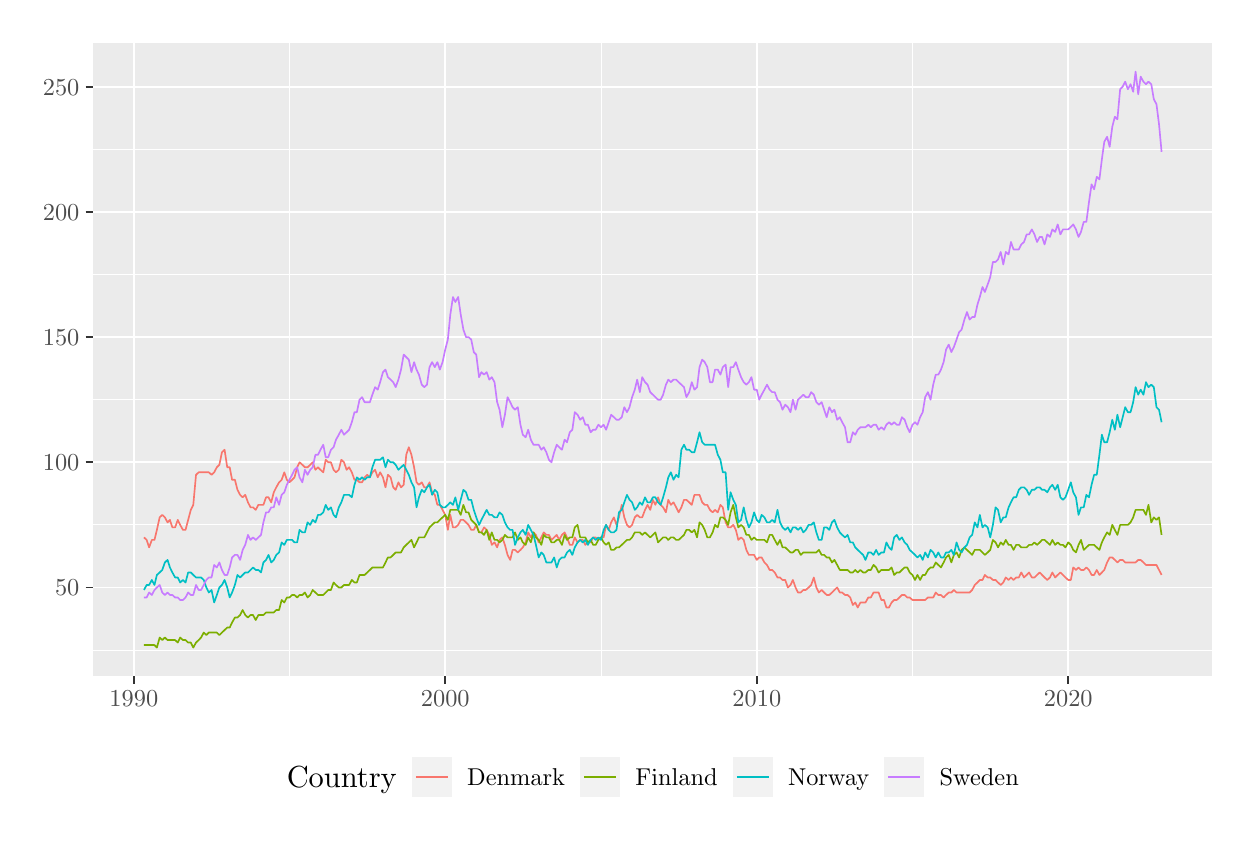
\begin{tikzpicture}[x=1pt,y=1pt]
\definecolor{fillColor}{RGB}{255,255,255}
\path[use as bounding box,fill=fillColor,fill opacity=0.00] (0,0) rectangle (433.62,289.08);
\begin{scope}
\path[clip] (  0.00,  0.00) rectangle (433.62,289.08);
\definecolor{drawColor}{RGB}{255,255,255}
\definecolor{fillColor}{RGB}{255,255,255}

\path[draw=drawColor,line width= 0.6pt,line join=round,line cap=round,fill=fillColor] (  0.00,  0.00) rectangle (433.62,289.08);
\end{scope}
\begin{scope}
\path[clip] ( 23.65, 54.68) rectangle (428.12,283.58);
\definecolor{fillColor}{gray}{0.92}

\path[fill=fillColor] ( 23.65, 54.68) rectangle (428.12,283.58);
\definecolor{drawColor}{RGB}{255,255,255}

\path[draw=drawColor,line width= 0.3pt,line join=round] ( 23.65, 64.18) --
	(428.12, 64.18);

\path[draw=drawColor,line width= 0.3pt,line join=round] ( 23.65,109.41) --
	(428.12,109.41);

\path[draw=drawColor,line width= 0.3pt,line join=round] ( 23.65,154.65) --
	(428.12,154.65);

\path[draw=drawColor,line width= 0.3pt,line join=round] ( 23.65,199.89) --
	(428.12,199.89);

\path[draw=drawColor,line width= 0.3pt,line join=round] ( 23.65,245.13) --
	(428.12,245.13);

\path[draw=drawColor,line width= 0.3pt,line join=round] ( 94.64, 54.68) --
	( 94.64,283.58);

\path[draw=drawColor,line width= 0.3pt,line join=round] (207.19, 54.68) --
	(207.19,283.58);

\path[draw=drawColor,line width= 0.3pt,line join=round] (319.75, 54.68) --
	(319.75,283.58);

\path[draw=drawColor,line width= 0.6pt,line join=round] ( 23.65, 86.79) --
	(428.12, 86.79);

\path[draw=drawColor,line width= 0.6pt,line join=round] ( 23.65,132.03) --
	(428.12,132.03);

\path[draw=drawColor,line width= 0.6pt,line join=round] ( 23.65,177.27) --
	(428.12,177.27);

\path[draw=drawColor,line width= 0.6pt,line join=round] ( 23.65,222.51) --
	(428.12,222.51);

\path[draw=drawColor,line width= 0.6pt,line join=round] ( 23.65,267.75) --
	(428.12,267.75);

\path[draw=drawColor,line width= 0.6pt,line join=round] ( 38.36, 54.68) --
	( 38.36,283.58);

\path[draw=drawColor,line width= 0.6pt,line join=round] (150.91, 54.68) --
	(150.91,283.58);

\path[draw=drawColor,line width= 0.6pt,line join=round] (263.48, 54.68) --
	(263.48,283.58);

\path[draw=drawColor,line width= 0.6pt,line join=round] (376.02, 54.68) --
	(376.02,283.58);
\definecolor{drawColor}{RGB}{248,118,109}

\path[draw=drawColor,line width= 0.6pt,line join=round] ( 42.03,104.89) --
	( 42.99,103.98) --
	( 43.88,101.27) --
	( 44.87,103.98) --
	( 45.82,103.98) --
	( 46.69,107.60) --
	( 47.70,112.13) --
	( 48.63,113.03) --
	( 49.58,112.13) --
	( 50.54,110.32) --
	( 51.40,111.22) --
	( 52.29,108.51) --
	( 53.28,108.51) --
	( 54.24,111.22) --
	( 55.10,109.41) --
	( 56.12,107.60) --
	( 57.04,107.60) --
	( 57.99,111.22) --
	( 58.95,114.84) --
	( 59.84,116.65) --
	( 60.83,127.51) --
	( 61.79,128.41) --
	( 62.65,128.41) --
	( 63.63,128.41) --
	( 64.56,128.41) --
	( 65.45,128.41) --
	( 66.44,127.51) --
	( 67.39,128.41) --
	( 68.35,130.22) --
	( 69.27,131.13) --
	( 70.20,135.65) --
	( 71.15,136.56) --
	( 72.11,130.22) --
	( 73.00,130.22) --
	( 73.87,125.70) --
	( 74.88,125.70) --
	( 75.81,122.08) --
	( 76.76,120.27) --
	( 77.69,119.37) --
	( 78.61,120.27) --
	( 79.60,117.56) --
	( 80.52,115.75) --
	( 81.42,115.75) --
	( 82.40,114.84) --
	( 83.36,116.65) --
	( 84.31,116.65) --
	( 85.18,116.65) --
	( 86.13,119.37) --
	( 87.02,119.37) --
	( 88.01,117.56) --
	( 88.93,121.18) --
	( 89.83,122.98) --
	( 90.85,124.79) --
	( 91.77,125.70) --
	( 92.73,128.41) --
	( 93.65,125.70) --
	( 94.57,124.79) --
	( 95.56,125.70) --
	( 96.42,126.60) --
	( 97.38,130.22) --
	( 98.24,132.03) --
	( 99.26,131.13) --
	(100.18,130.22) --
	(101.14,130.22) --
	(102.09,131.13) --
	(102.99,132.03) --
	(103.97,129.32) --
	(104.90,130.22) --
	(105.79,129.32) --
	(106.81,128.41) --
	(107.70,132.94) --
	(108.60,132.03) --
	(109.58,132.03) --
	(110.54,129.32) --
	(111.40,128.41) --
	(112.42,129.32) --
	(113.34,132.94) --
	(114.30,132.03) --
	(115.25,129.32) --
	(116.15,130.22) --
	(117.13,128.41) --
	(118.09,125.70) --
	(118.95,125.70) --
	(119.91,124.79) --
	(120.83,124.79) --
	(121.75,126.60) --
	(122.71,127.51) --
	(123.66,126.60) --
	(124.56,128.41) --
	(125.54,129.32) --
	(126.50,126.60) --
	(127.36,128.41) --
	(128.38,126.60) --
	(129.30,122.98) --
	(130.17,127.51) --
	(131.15,126.60) --
	(132.08,122.98) --
	(132.97,122.08) --
	(133.96,124.79) --
	(134.91,122.98) --
	(135.87,123.89) --
	(136.79,134.75) --
	(137.72,137.46) --
	(138.67,134.75) --
	(139.63,130.22) --
	(140.52,124.79) --
	(141.38,123.89) --
	(142.40,124.79) --
	(143.33,122.98) --
	(144.28,122.98) --
	(145.21,124.79) --
	(146.13,121.18) --
	(147.12,120.27) --
	(148.04,116.65) --
	(148.93,116.65) --
	(149.92,114.84) --
	(150.88,113.03) --
	(151.83,107.60) --
	(152.72,113.03) --
	(153.68,108.51) --
	(154.54,108.51) --
	(155.56,109.41) --
	(156.48,111.22) --
	(157.44,111.22) --
	(158.40,110.32) --
	(159.29,109.41) --
	(160.28,107.60) --
	(161.20,107.60) --
	(162.09,109.41) --
	(163.11,106.70) --
	(163.97,106.70) --
	(164.90,108.51) --
	(165.85,107.60) --
	(166.81,105.79) --
	(167.70,102.18) --
	(168.69,103.08) --
	(169.64,101.27) --
	(170.51,103.98) --
	(171.52,104.89) --
	(172.45,102.18) --
	(173.40, 98.56) --
	(174.36, 96.75) --
	(175.22,100.37) --
	(176.11,100.37) --
	(177.10, 99.46) --
	(178.06,100.37) --
	(178.92,101.27) --
	(179.94,103.08) --
	(180.86,106.70) --
	(181.82,104.89) --
	(182.77,106.70) --
	(183.66,105.79) --
	(184.65,103.08) --
	(185.61,104.89) --
	(186.47,106.70) --
	(187.42,105.79) --
	(188.35,105.79) --
	(189.27,103.98) --
	(190.23,104.89) --
	(191.18,105.79) --
	(192.08,103.98) --
	(193.06,105.79) --
	(194.02,106.70) --
	(194.88,104.89) --
	(195.90,102.18) --
	(196.82,102.18) --
	(197.69,104.89) --
	(198.70,103.08) --
	(199.63,103.98) --
	(200.58,103.98) --
	(201.51,102.18) --
	(202.43,103.08) --
	(203.42,103.08) --
	(204.34,104.89) --
	(205.24,104.89) --
	(206.22,103.98) --
	(207.18,104.89) --
	(208.13,104.89) --
	(209.00,109.41) --
	(209.95,107.60) --
	(210.84,110.32) --
	(211.83,112.13) --
	(212.76,109.41) --
	(213.65,112.13) --
	(214.67,116.65) --
	(215.59,112.13) --
	(216.55,109.41) --
	(217.47,108.51) --
	(218.40,109.41) --
	(219.38,112.13) --
	(220.24,113.03) --
	(221.20,112.13) --
	(222.06,112.13) --
	(223.08,114.84) --
	(224.00,116.65) --
	(224.96,114.84) --
	(225.91,118.46) --
	(226.81,116.65) --
	(227.79,119.37) --
	(228.72,116.65) --
	(229.61,115.75) --
	(230.63,113.94) --
	(231.49,118.46) --
	(232.42,116.65) --
	(233.37,117.56) --
	(234.33,115.75) --
	(235.22,113.94) --
	(236.21,115.75) --
	(237.16,118.46) --
	(238.03,118.46) --
	(239.04,117.56) --
	(239.97,116.65) --
	(240.92,120.27) --
	(241.88,120.27) --
	(242.77,120.27) --
	(243.73,117.56) --
	(244.65,116.65) --
	(245.58,116.65) --
	(246.53,114.84) --
	(247.49,113.94) --
	(248.38,114.84) --
	(249.37,113.94) --
	(250.32,116.65) --
	(251.18,115.75) --
	(252.20,110.32) --
	(253.13,108.51) --
	(253.99,108.51) --
	(254.97,109.41) --
	(255.90,107.60) --
	(256.79,103.98) --
	(257.78,104.89) --
	(258.73,103.98) --
	(259.69,100.37) --
	(260.61, 98.56) --
	(261.54, 98.56) --
	(262.49, 98.56) --
	(263.45, 96.75) --
	(264.34, 97.65) --
	(265.21, 97.65) --
	(266.22, 95.84) --
	(267.15, 94.94) --
	(268.10, 93.13) --
	(269.03, 93.13) --
	(269.95, 92.22) --
	(270.94, 90.41) --
	(271.86, 90.41) --
	(272.76, 89.51) --
	(273.74, 89.51) --
	(274.70, 86.79) --
	(275.65, 87.70) --
	(276.51, 89.51) --
	(277.47, 86.79) --
	(278.36, 84.98) --
	(279.35, 84.98) --
	(280.27, 85.89) --
	(281.17, 85.89) --
	(282.19, 86.79) --
	(283.11, 87.70) --
	(284.07, 90.41) --
	(284.99, 86.79) --
	(285.91, 84.98) --
	(286.90, 85.89) --
	(287.79, 84.98) --
	(288.72, 84.08) --
	(289.67, 84.08) --
	(290.63, 84.98) --
	(291.52, 85.89) --
	(292.51, 86.79) --
	(293.46, 84.98) --
	(294.33, 84.98) --
	(295.34, 84.08) --
	(296.27, 84.08) --
	(297.22, 83.18) --
	(298.18, 80.46) --
	(299.04, 81.37) --
	(299.94, 79.56) --
	(300.92, 81.37) --
	(301.88, 81.37) --
	(302.74, 81.37) --
	(303.76, 83.18) --
	(304.68, 83.18) --
	(305.64, 84.98) --
	(306.59, 84.98) --
	(307.49, 84.98) --
	(308.47, 82.27) --
	(309.43, 82.27) --
	(310.29, 79.56) --
	(311.25, 79.56) --
	(312.17, 81.37) --
	(313.09, 82.27) --
	(314.05, 82.27) --
	(315.00, 83.18) --
	(315.90, 84.08) --
	(316.88, 84.08) --
	(317.84, 83.18) --
	(318.70, 83.18) --
	(319.72, 82.27) --
	(320.64, 82.27) --
	(321.51, 82.27) --
	(322.49, 82.27) --
	(323.42, 82.27) --
	(324.31, 82.27) --
	(325.30, 83.18) --
	(326.25, 83.18) --
	(327.21, 83.18) --
	(328.13, 84.98) --
	(329.06, 84.08) --
	(330.01, 84.08) --
	(330.97, 83.18) --
	(331.86, 84.08) --
	(332.82, 84.98) --
	(333.77, 84.98) --
	(334.67, 85.89) --
	(335.65, 84.98) --
	(336.58, 84.98) --
	(337.47, 84.98) --
	(338.49, 84.98) --
	(339.41, 84.98) --
	(340.37, 84.98) --
	(341.29, 85.89) --
	(342.22, 87.70) --
	(343.20, 88.60) --
	(344.06, 89.51) --
	(345.02, 89.51) --
	(345.88, 91.32) --
	(346.90, 90.41) --
	(347.82, 90.41) --
	(348.78, 89.51) --
	(349.74, 89.51) --
	(350.63, 88.60) --
	(351.61, 87.70) --
	(352.54, 88.60) --
	(353.43, 90.41) --
	(354.45, 89.51) --
	(355.31, 90.41) --
	(356.24, 89.51) --
	(357.19, 90.41) --
	(358.15, 90.41) --
	(359.04, 92.22) --
	(360.03, 90.41) --
	(360.98, 91.32) --
	(361.85, 92.22) --
	(362.86, 90.41) --
	(363.79, 90.41) --
	(364.74, 91.32) --
	(365.70, 92.22) --
	(366.56, 91.32) --
	(367.45, 90.41) --
	(368.44, 89.51) --
	(369.40, 90.41) --
	(370.26, 92.22) --
	(371.28, 90.41) --
	(372.20, 91.32) --
	(373.16, 92.22) --
	(374.11, 91.32) --
	(375.00, 90.41) --
	(375.99, 89.51) --
	(376.95, 89.51) --
	(377.81, 94.03) --
	(378.80, 93.13) --
	(379.72, 94.03) --
	(380.61, 93.13) --
	(381.60, 93.13) --
	(382.55, 94.03) --
	(383.51, 93.13) --
	(384.43, 91.32) --
	(385.36, 91.32) --
	(386.31, 93.13) --
	(387.27, 91.32) --
	(388.16, 92.22) --
	(389.03, 93.13) --
	(390.04, 95.84) --
	(390.97, 97.65) --
	(391.92, 97.65) --
	(392.85, 96.75) --
	(393.77, 95.84) --
	(394.76, 96.75) --
	(395.68, 96.75) --
	(396.58, 95.84) --
	(397.56, 95.84) --
	(398.52, 95.84) --
	(399.47, 95.84) --
	(400.34, 95.84) --
	(401.29, 96.75) --
	(402.18, 96.75) --
	(403.17, 95.84) --
	(404.10, 94.94) --
	(404.99, 94.94) --
	(406.01, 94.94) --
	(406.93, 94.94) --
	(407.89, 94.94) --
	(408.81, 93.13) --
	(409.73, 91.32);
\definecolor{drawColor}{RGB}{124,174,0}

\path[draw=drawColor,line width= 0.6pt,line join=round] ( 42.03, 65.98) --
	( 42.99, 65.98) --
	( 43.88, 65.98) --
	( 44.87, 65.98) --
	( 45.82, 65.98) --
	( 46.69, 65.08) --
	( 47.70, 68.70) --
	( 48.63, 67.79) --
	( 49.58, 68.70) --
	( 50.54, 67.79) --
	( 51.40, 67.79) --
	( 52.29, 67.79) --
	( 53.28, 67.79) --
	( 54.24, 66.89) --
	( 55.10, 68.70) --
	( 56.12, 67.79) --
	( 57.04, 67.79) --
	( 57.99, 66.89) --
	( 58.95, 66.89) --
	( 59.84, 65.08) --
	( 60.83, 66.89) --
	( 61.79, 67.79) --
	( 62.65, 68.70) --
	( 63.63, 70.51) --
	( 64.56, 69.60) --
	( 65.45, 70.51) --
	( 66.44, 70.51) --
	( 67.39, 70.51) --
	( 68.35, 70.51) --
	( 69.27, 69.60) --
	( 70.20, 70.51) --
	( 71.15, 71.41) --
	( 72.11, 72.32) --
	( 73.00, 72.32) --
	( 73.87, 74.13) --
	( 74.88, 75.94) --
	( 75.81, 75.94) --
	( 76.76, 76.84) --
	( 77.69, 78.65) --
	( 78.61, 76.84) --
	( 79.60, 75.94) --
	( 80.52, 76.84) --
	( 81.42, 76.84) --
	( 82.40, 75.03) --
	( 83.36, 76.84) --
	( 84.31, 76.84) --
	( 85.18, 76.84) --
	( 86.13, 77.75) --
	( 87.02, 77.75) --
	( 88.01, 77.75) --
	( 88.93, 77.75) --
	( 89.83, 78.65) --
	( 90.85, 78.65) --
	( 91.77, 82.27) --
	( 92.73, 81.37) --
	( 93.65, 83.18) --
	( 94.57, 83.18) --
	( 95.56, 84.08) --
	( 96.42, 84.08) --
	( 97.38, 83.18) --
	( 98.24, 84.08) --
	( 99.26, 84.08) --
	(100.18, 84.98) --
	(101.14, 83.18) --
	(102.09, 84.08) --
	(102.99, 85.89) --
	(103.97, 84.98) --
	(104.90, 84.08) --
	(105.79, 84.08) --
	(106.81, 84.08) --
	(107.70, 84.98) --
	(108.60, 85.89) --
	(109.58, 85.89) --
	(110.54, 88.60) --
	(111.40, 87.70) --
	(112.42, 86.79) --
	(113.34, 86.79) --
	(114.30, 87.70) --
	(115.25, 87.70) --
	(116.15, 87.70) --
	(117.13, 89.51) --
	(118.09, 88.60) --
	(118.95, 88.60) --
	(119.91, 91.32) --
	(120.83, 91.32) --
	(121.75, 91.32) --
	(122.71, 92.22) --
	(123.66, 93.13) --
	(124.56, 94.03) --
	(125.54, 94.03) --
	(126.50, 94.03) --
	(127.36, 94.03) --
	(128.38, 94.03) --
	(129.30, 95.84) --
	(130.17, 97.65) --
	(131.15, 97.65) --
	(132.08, 98.56) --
	(132.97, 99.46) --
	(133.96, 99.46) --
	(134.91, 99.46) --
	(135.87,101.27) --
	(136.79,102.18) --
	(137.72,103.08) --
	(138.67,103.98) --
	(139.63,101.27) --
	(140.52,103.08) --
	(141.38,104.89) --
	(142.40,104.89) --
	(143.33,104.89) --
	(144.28,106.70) --
	(145.21,108.51) --
	(146.13,109.41) --
	(147.12,110.32) --
	(148.04,110.32) --
	(148.93,111.22) --
	(149.92,112.13) --
	(150.88,113.03) --
	(151.83,111.22) --
	(152.72,114.84) --
	(153.68,114.84) --
	(154.54,114.84) --
	(155.56,114.84) --
	(156.48,113.03) --
	(157.44,116.65) --
	(158.40,113.94) --
	(159.29,113.94) --
	(160.28,111.22) --
	(161.20,110.32) --
	(162.09,109.41) --
	(163.11,106.70) --
	(163.97,106.70) --
	(164.90,105.79) --
	(165.85,107.60) --
	(166.81,103.98) --
	(167.70,106.70) --
	(168.69,103.98) --
	(169.64,103.98) --
	(170.51,103.08) --
	(171.52,103.98) --
	(172.45,105.79) --
	(173.40,104.89) --
	(174.36,104.89) --
	(175.22,104.89) --
	(176.11,106.70) --
	(177.10,103.98) --
	(178.06,104.89) --
	(178.92,103.08) --
	(179.94,102.18) --
	(180.86,104.89) --
	(181.82,103.08) --
	(182.77,106.70) --
	(183.66,104.89) --
	(184.65,103.98) --
	(185.61,102.18) --
	(186.47,105.79) --
	(187.42,104.89) --
	(188.35,104.89) --
	(189.27,103.08) --
	(190.23,103.08) --
	(191.18,103.98) --
	(192.08,103.98) --
	(193.06,102.18) --
	(194.02,105.79) --
	(194.88,103.98) --
	(195.90,104.89) --
	(196.82,104.89) --
	(197.69,108.51) --
	(198.70,109.41) --
	(199.63,104.89) --
	(200.58,104.89) --
	(201.51,104.89) --
	(202.43,103.08) --
	(203.42,103.98) --
	(204.34,102.18) --
	(205.24,102.18) --
	(206.22,103.98) --
	(207.18,104.89) --
	(208.13,103.08) --
	(209.00,102.18) --
	(209.95,103.08) --
	(210.84,100.37) --
	(211.83,100.37) --
	(212.76,101.27) --
	(213.65,101.27) --
	(214.67,102.18) --
	(215.59,103.08) --
	(216.55,103.98) --
	(217.47,103.98) --
	(218.40,104.89) --
	(219.38,106.70) --
	(220.24,106.70) --
	(221.20,106.70) --
	(222.06,105.79) --
	(223.08,106.70) --
	(224.00,105.79) --
	(224.96,104.89) --
	(225.91,105.79) --
	(226.81,106.70) --
	(227.79,103.08) --
	(228.72,103.98) --
	(229.61,104.89) --
	(230.63,104.89) --
	(231.49,103.98) --
	(232.42,104.89) --
	(233.37,104.89) --
	(234.33,103.98) --
	(235.22,103.98) --
	(236.21,104.89) --
	(237.16,105.79) --
	(238.03,107.60) --
	(239.04,107.60) --
	(239.97,106.70) --
	(240.92,107.60) --
	(241.88,104.89) --
	(242.77,110.32) --
	(243.73,109.41) --
	(244.65,107.60) --
	(245.58,104.89) --
	(246.53,104.89) --
	(247.49,106.70) --
	(248.38,109.41) --
	(249.37,108.51) --
	(250.32,112.13) --
	(251.18,112.13) --
	(252.20,111.22) --
	(253.13,109.41) --
	(253.99,113.94) --
	(254.97,116.65) --
	(255.90,112.13) --
	(256.79,108.51) --
	(257.78,109.41) --
	(258.73,108.51) --
	(259.69,105.79) --
	(260.61,105.79) --
	(261.54,103.98) --
	(262.49,104.89) --
	(263.45,103.98) --
	(264.34,103.98) --
	(265.21,103.98) --
	(266.22,103.98) --
	(267.15,103.08) --
	(268.10,105.79) --
	(269.03,105.79) --
	(269.95,103.98) --
	(270.94,102.18) --
	(271.86,103.98) --
	(272.76,101.27) --
	(273.74,101.27) --
	(274.70,100.37) --
	(275.65, 99.46) --
	(276.51, 99.46) --
	(277.47,100.37) --
	(278.36,100.37) --
	(279.35, 98.56) --
	(280.27, 99.46) --
	(281.17, 99.46) --
	(282.19, 99.46) --
	(283.11, 99.46) --
	(284.07, 99.46) --
	(284.99, 99.46) --
	(285.91,100.37) --
	(286.90, 98.56) --
	(287.79, 98.56) --
	(288.72, 97.65) --
	(289.67, 97.65) --
	(290.63, 95.84) --
	(291.52, 96.75) --
	(292.51, 94.94) --
	(293.46, 93.13) --
	(294.33, 93.13) --
	(295.34, 93.13) --
	(296.27, 93.13) --
	(297.22, 92.22) --
	(298.18, 92.22) --
	(299.04, 93.13) --
	(299.94, 92.22) --
	(300.92, 93.13) --
	(301.88, 92.22) --
	(302.74, 92.22) --
	(303.76, 93.13) --
	(304.68, 93.13) --
	(305.64, 94.94) --
	(306.59, 94.03) --
	(307.49, 92.22) --
	(308.47, 93.13) --
	(309.43, 93.13) --
	(310.29, 93.13) --
	(311.25, 93.13) --
	(312.17, 94.03) --
	(313.09, 91.32) --
	(314.05, 92.22) --
	(315.00, 92.22) --
	(315.90, 93.13) --
	(316.88, 94.03) --
	(317.84, 94.03) --
	(318.70, 92.22) --
	(319.72, 91.32) --
	(320.64, 89.51) --
	(321.51, 91.32) --
	(322.49, 89.51) --
	(323.42, 91.32) --
	(324.31, 91.32) --
	(325.30, 93.13) --
	(326.25, 94.03) --
	(327.21, 94.03) --
	(328.13, 95.84) --
	(329.06, 94.94) --
	(330.01, 94.03) --
	(330.97, 95.84) --
	(331.86, 97.65) --
	(332.82, 98.56) --
	(333.77, 95.84) --
	(334.67, 98.56) --
	(335.65, 99.46) --
	(336.58, 97.65) --
	(337.47,100.37) --
	(338.49,101.27) --
	(339.41,100.37) --
	(340.37, 99.46) --
	(341.29, 98.56) --
	(342.22,100.37) --
	(343.20,100.37) --
	(344.06,100.37) --
	(345.02, 99.46) --
	(345.88, 98.56) --
	(346.90, 99.46) --
	(347.82,100.37) --
	(348.78,103.98) --
	(349.74,103.08) --
	(350.63,101.27) --
	(351.61,103.08) --
	(352.54,102.18) --
	(353.43,103.98) --
	(354.45,102.18) --
	(355.31,102.18) --
	(356.24,100.37) --
	(357.19,102.18) --
	(358.15,102.18) --
	(359.04,101.27) --
	(360.03,101.27) --
	(360.98,101.27) --
	(361.85,102.18) --
	(362.86,102.18) --
	(363.79,103.08) --
	(364.74,102.18) --
	(365.70,103.08) --
	(366.56,103.98) --
	(367.45,103.98) --
	(368.44,103.08) --
	(369.40,102.18) --
	(370.26,103.98) --
	(371.28,102.18) --
	(372.20,103.08) --
	(373.16,102.18) --
	(374.11,102.18) --
	(375.00,101.27) --
	(375.99,103.08) --
	(376.95,102.18) --
	(377.81,100.37) --
	(378.80, 99.46) --
	(379.72,102.18) --
	(380.61,103.98) --
	(381.60,100.37) --
	(382.55,101.27) --
	(383.51,102.18) --
	(384.43,102.18) --
	(385.36,102.18) --
	(386.31,101.27) --
	(387.27,100.37) --
	(388.16,103.08) --
	(389.03,104.89) --
	(390.04,106.70) --
	(390.97,105.79) --
	(391.92,109.41) --
	(392.85,107.60) --
	(393.77,105.79) --
	(394.76,109.41) --
	(395.68,109.41) --
	(396.58,109.41) --
	(397.56,109.41) --
	(398.52,110.32) --
	(399.47,112.13) --
	(400.34,114.84) --
	(401.29,114.84) --
	(402.18,114.84) --
	(403.17,114.84) --
	(404.10,113.03) --
	(404.99,116.65) --
	(406.01,110.32) --
	(406.93,112.13) --
	(407.89,111.22) --
	(408.81,112.13) --
	(409.73,105.79);
\definecolor{drawColor}{RGB}{0,191,196}

\path[draw=drawColor,line width= 0.6pt,line join=round] ( 42.03, 85.89) --
	( 42.99, 87.70) --
	( 43.88, 87.70) --
	( 44.87, 89.51) --
	( 45.82, 87.70) --
	( 46.69, 91.32) --
	( 47.70, 92.22) --
	( 48.63, 93.13) --
	( 49.58, 95.84) --
	( 50.54, 96.75) --
	( 51.40, 94.03) --
	( 52.29, 92.22) --
	( 53.28, 90.41) --
	( 54.24, 90.41) --
	( 55.10, 88.60) --
	( 56.12, 89.51) --
	( 57.04, 88.60) --
	( 57.99, 92.22) --
	( 58.95, 92.22) --
	( 59.84, 91.32) --
	( 60.83, 90.41) --
	( 61.79, 90.41) --
	( 62.65, 90.41) --
	( 63.63, 89.51) --
	( 64.56, 86.79) --
	( 65.45, 84.98) --
	( 66.44, 85.89) --
	( 67.39, 81.37) --
	( 68.35, 84.08) --
	( 69.27, 86.79) --
	( 70.20, 87.70) --
	( 71.15, 89.51) --
	( 72.11, 86.79) --
	( 73.00, 83.18) --
	( 73.87, 84.98) --
	( 74.88, 87.70) --
	( 75.81, 91.32) --
	( 76.76, 90.41) --
	( 77.69, 91.32) --
	( 78.61, 92.22) --
	( 79.60, 92.22) --
	( 80.52, 93.13) --
	( 81.42, 94.03) --
	( 82.40, 93.13) --
	( 83.36, 93.13) --
	( 84.31, 92.22) --
	( 85.18, 95.84) --
	( 86.13, 96.75) --
	( 87.02, 98.56) --
	( 88.01, 95.84) --
	( 88.93, 96.75) --
	( 89.83, 98.56) --
	( 90.85, 99.46) --
	( 91.77,103.08) --
	( 92.73,102.18) --
	( 93.65,103.98) --
	( 94.57,103.98) --
	( 95.56,103.98) --
	( 96.42,103.08) --
	( 97.38,103.08) --
	( 98.24,107.60) --
	( 99.26,106.70) --
	(100.18,106.70) --
	(101.14,110.32) --
	(102.09,109.41) --
	(102.99,111.22) --
	(103.97,110.32) --
	(104.90,113.03) --
	(105.79,113.03) --
	(106.81,113.94) --
	(107.70,116.65) --
	(108.60,114.84) --
	(109.58,115.75) --
	(110.54,113.03) --
	(111.40,112.13) --
	(112.42,115.75) --
	(113.34,117.56) --
	(114.30,120.27) --
	(115.25,120.27) --
	(116.15,120.27) --
	(117.13,119.37) --
	(118.09,123.89) --
	(118.95,126.60) --
	(119.91,125.70) --
	(120.83,126.60) --
	(121.75,125.70) --
	(122.71,126.60) --
	(123.66,126.60) --
	(124.56,130.22) --
	(125.54,132.94) --
	(126.50,132.94) --
	(127.36,132.94) --
	(128.38,133.84) --
	(129.30,130.22) --
	(130.17,132.94) --
	(131.15,132.03) --
	(132.08,132.03) --
	(132.97,131.13) --
	(133.96,129.32) --
	(134.91,130.22) --
	(135.87,131.13) --
	(136.79,129.32) --
	(137.72,127.51) --
	(138.67,124.79) --
	(139.63,122.98) --
	(140.52,115.75) --
	(141.38,119.37) --
	(142.40,122.08) --
	(143.33,121.18) --
	(144.28,122.98) --
	(145.21,123.89) --
	(146.13,120.27) --
	(147.12,122.08) --
	(148.04,121.18) --
	(148.93,116.65) --
	(149.92,115.75) --
	(150.88,115.75) --
	(151.83,116.65) --
	(152.72,117.56) --
	(153.68,116.65) --
	(154.54,119.37) --
	(155.56,114.84) --
	(156.48,118.46) --
	(157.44,122.08) --
	(158.40,121.18) --
	(159.29,118.46) --
	(160.28,118.46) --
	(161.20,114.84) --
	(162.09,112.13) --
	(163.11,109.41) --
	(163.97,111.22) --
	(164.90,113.03) --
	(165.85,114.84) --
	(166.81,113.03) --
	(167.70,113.03) --
	(168.69,112.13) --
	(169.64,112.13) --
	(170.51,113.94) --
	(171.52,113.03) --
	(172.45,110.32) --
	(173.40,108.51) --
	(174.36,107.60) --
	(175.22,107.60) --
	(176.11,102.18) --
	(177.10,104.89) --
	(178.06,106.70) --
	(178.92,107.60) --
	(179.94,105.79) --
	(180.86,109.41) --
	(181.82,107.60) --
	(182.77,105.79) --
	(183.66,102.18) --
	(184.65, 97.65) --
	(185.61, 99.46) --
	(186.47, 98.56) --
	(187.42, 95.84) --
	(188.35, 95.84) --
	(189.27, 95.84) --
	(190.23, 97.65) --
	(191.18, 94.03) --
	(192.08, 96.75) --
	(193.06, 97.65) --
	(194.02, 97.65) --
	(194.88, 99.46) --
	(195.90,100.37) --
	(196.82, 98.56) --
	(197.69,101.27) --
	(198.70,103.08) --
	(199.63,103.98) --
	(200.58,103.08) --
	(201.51,103.98) --
	(202.43,102.18) --
	(203.42,103.98) --
	(204.34,104.89) --
	(205.24,103.98) --
	(206.22,104.89) --
	(207.18,103.98) --
	(208.13,107.60) --
	(209.00,109.41) --
	(209.95,107.60) --
	(210.84,106.70) --
	(211.83,106.70) --
	(212.76,107.60) --
	(213.65,113.94) --
	(214.67,114.84) --
	(215.59,117.56) --
	(216.55,120.27) --
	(217.47,118.46) --
	(218.40,117.56) --
	(219.38,114.84) --
	(220.24,115.75) --
	(221.20,117.56) --
	(222.06,116.65) --
	(223.08,119.37) --
	(224.00,117.56) --
	(224.96,117.56) --
	(225.91,119.37) --
	(226.81,119.37) --
	(227.79,117.56) --
	(228.72,116.65) --
	(229.61,119.37) --
	(230.63,122.98) --
	(231.49,126.60) --
	(232.42,128.41) --
	(233.37,125.70) --
	(234.33,127.51) --
	(235.22,126.60) --
	(236.21,136.56) --
	(237.16,138.37) --
	(238.03,136.56) --
	(239.04,136.56) --
	(239.97,135.65) --
	(240.92,135.65) --
	(241.88,139.27) --
	(242.77,142.89) --
	(243.73,139.27) --
	(244.65,138.37) --
	(245.58,138.37) --
	(246.53,138.37) --
	(247.49,138.37) --
	(248.38,138.37) --
	(249.37,134.75) --
	(250.32,132.94) --
	(251.18,128.41) --
	(252.20,128.41) --
	(253.13,114.84) --
	(253.99,121.18) --
	(254.97,118.46) --
	(255.90,116.65) --
	(256.79,110.32) --
	(257.78,111.22) --
	(258.73,115.75) --
	(259.69,111.22) --
	(260.61,108.51) --
	(261.54,110.32) --
	(262.49,113.94) --
	(263.45,111.22) --
	(264.34,110.32) --
	(265.21,113.03) --
	(266.22,112.13) --
	(267.15,110.32) --
	(268.10,110.32) --
	(269.03,111.22) --
	(269.95,110.32) --
	(270.94,114.84) --
	(271.86,110.32) --
	(272.76,108.51) --
	(273.74,107.60) --
	(274.70,108.51) --
	(275.65,106.70) --
	(276.51,108.51) --
	(277.47,108.51) --
	(278.36,107.60) --
	(279.35,108.51) --
	(280.27,106.70) --
	(281.17,107.60) --
	(282.19,109.41) --
	(283.11,109.41) --
	(284.07,110.32) --
	(284.99,106.70) --
	(285.91,103.98) --
	(286.90,103.98) --
	(287.79,108.51) --
	(288.72,108.51) --
	(289.67,107.60) --
	(290.63,110.32) --
	(291.52,111.22) --
	(292.51,108.51) --
	(293.46,106.70) --
	(294.33,105.79) --
	(295.34,104.89) --
	(296.27,105.79) --
	(297.22,103.08) --
	(298.18,103.08) --
	(299.04,101.27) --
	(299.94,100.37) --
	(300.92, 99.46) --
	(301.88, 98.56) --
	(302.74, 96.75) --
	(303.76, 99.46) --
	(304.68, 99.46) --
	(305.64, 98.56) --
	(306.59,100.37) --
	(307.49, 98.56) --
	(308.47, 99.46) --
	(309.43, 99.46) --
	(310.29,103.08) --
	(311.25,101.27) --
	(312.17,100.37) --
	(313.09,104.89) --
	(314.05,105.79) --
	(315.00,103.98) --
	(315.90,104.89) --
	(316.88,103.08) --
	(317.84,102.18) --
	(318.70,100.37) --
	(319.72, 99.46) --
	(320.64, 98.56) --
	(321.51, 97.65) --
	(322.49, 98.56) --
	(323.42, 96.75) --
	(324.31, 99.46) --
	(325.30, 97.65) --
	(326.25,100.37) --
	(327.21, 99.46) --
	(328.13, 97.65) --
	(329.06, 99.46) --
	(330.01, 97.65) --
	(330.97, 97.65) --
	(331.86, 99.46) --
	(332.82, 99.46) --
	(333.77,100.37) --
	(334.67, 98.56) --
	(335.65,103.08) --
	(336.58,100.37) --
	(337.47, 99.46) --
	(338.49,101.27) --
	(339.41,102.18) --
	(340.37,104.89) --
	(341.29,105.79) --
	(342.22,110.32) --
	(343.20,108.51) --
	(344.06,113.03) --
	(345.02,108.51) --
	(345.88,109.41) --
	(346.90,108.51) --
	(347.82,104.89) --
	(348.78,109.41) --
	(349.74,115.75) --
	(350.63,114.84) --
	(351.61,110.32) --
	(352.54,112.13) --
	(353.43,112.13) --
	(354.45,115.75) --
	(355.31,117.56) --
	(356.24,119.37) --
	(357.19,119.37) --
	(358.15,122.08) --
	(359.04,122.98) --
	(360.03,122.98) --
	(360.98,122.08) --
	(361.85,120.27) --
	(362.86,122.08) --
	(363.79,122.08) --
	(364.74,122.98) --
	(365.70,122.98) --
	(366.56,122.08) --
	(367.45,122.08) --
	(368.44,121.18) --
	(369.40,122.98) --
	(370.26,123.89) --
	(371.28,122.08) --
	(372.20,123.89) --
	(373.16,119.37) --
	(374.11,118.46) --
	(375.00,119.37) --
	(375.99,122.08) --
	(376.95,124.79) --
	(377.81,121.18) --
	(378.80,119.37) --
	(379.72,113.03) --
	(380.61,115.75) --
	(381.60,115.75) --
	(382.55,120.27) --
	(383.51,119.37) --
	(384.43,123.89) --
	(385.36,127.51) --
	(386.31,127.51) --
	(387.27,134.75) --
	(388.16,141.98) --
	(389.03,139.27) --
	(390.04,139.27) --
	(390.97,142.89) --
	(391.92,147.41) --
	(392.85,143.79) --
	(393.77,149.22) --
	(394.76,144.70) --
	(395.68,148.32) --
	(396.58,151.94) --
	(397.56,150.13) --
	(398.52,150.13) --
	(399.47,153.75) --
	(400.34,159.18) --
	(401.29,156.46) --
	(402.18,158.27) --
	(403.17,156.46) --
	(404.10,160.98) --
	(404.99,159.18) --
	(406.01,160.08) --
	(406.93,159.18) --
	(407.89,151.94) --
	(408.81,151.03) --
	(409.73,146.51);
\definecolor{drawColor}{RGB}{199,124,255}

\path[draw=drawColor,line width= 0.6pt,line join=round] ( 42.03, 83.18) --
	( 42.99, 83.18) --
	( 43.88, 84.98) --
	( 44.87, 84.08) --
	( 45.82, 85.89) --
	( 46.69, 86.79) --
	( 47.70, 87.70) --
	( 48.63, 84.98) --
	( 49.58, 84.08) --
	( 50.54, 84.98) --
	( 51.40, 84.08) --
	( 52.29, 84.08) --
	( 53.28, 83.18) --
	( 54.24, 83.18) --
	( 55.10, 82.27) --
	( 56.12, 82.27) --
	( 57.04, 83.18) --
	( 57.99, 84.98) --
	( 58.95, 84.08) --
	( 59.84, 84.08) --
	( 60.83, 87.70) --
	( 61.79, 85.89) --
	( 62.65, 85.89) --
	( 63.63, 87.70) --
	( 64.56, 89.51) --
	( 65.45, 90.41) --
	( 66.44, 90.41) --
	( 67.39, 94.94) --
	( 68.35, 94.03) --
	( 69.27, 95.84) --
	( 70.20, 93.13) --
	( 71.15, 91.32) --
	( 72.11, 91.32) --
	( 73.00, 94.03) --
	( 73.87, 97.65) --
	( 74.88, 98.56) --
	( 75.81, 98.56) --
	( 76.76, 96.75) --
	( 77.69,100.37) --
	( 78.61,102.18) --
	( 79.60,105.79) --
	( 80.52,103.98) --
	( 81.42,104.89) --
	( 82.40,103.98) --
	( 83.36,104.89) --
	( 84.31,105.79) --
	( 85.18,110.32) --
	( 86.13,113.94) --
	( 87.02,113.94) --
	( 88.01,115.75) --
	( 88.93,115.75) --
	( 89.83,119.37) --
	( 90.85,116.65) --
	( 91.77,120.27) --
	( 92.73,121.18) --
	( 93.65,123.89) --
	( 94.57,125.70) --
	( 95.56,127.51) --
	( 96.42,129.32) --
	( 97.38,130.22) --
	( 98.24,126.60) --
	( 99.26,124.79) --
	(100.18,129.32) --
	(101.14,127.51) --
	(102.09,129.32) --
	(102.99,130.22) --
	(103.97,134.75) --
	(104.90,134.75) --
	(105.79,136.56) --
	(106.81,138.37) --
	(107.70,133.84) --
	(108.60,133.84) --
	(109.58,136.56) --
	(110.54,137.46) --
	(111.40,140.18) --
	(112.42,141.98) --
	(113.34,143.79) --
	(114.30,141.98) --
	(115.25,142.89) --
	(116.15,143.79) --
	(117.13,146.51) --
	(118.09,150.13) --
	(118.95,150.13) --
	(119.91,154.65) --
	(120.83,155.56) --
	(121.75,153.75) --
	(122.71,153.75) --
	(123.66,153.75) --
	(124.56,156.46) --
	(125.54,159.18) --
	(126.50,158.27) --
	(127.36,160.98) --
	(128.38,164.60) --
	(129.30,165.51) --
	(130.17,162.79) --
	(131.15,161.89) --
	(132.08,160.98) --
	(132.97,159.18) --
	(133.96,161.89) --
	(134.91,165.51) --
	(135.87,170.94) --
	(136.79,170.03) --
	(137.72,169.13) --
	(138.67,164.60) --
	(139.63,168.22) --
	(140.52,165.51) --
	(141.38,163.70) --
	(142.40,160.08) --
	(143.33,159.18) --
	(144.28,160.08) --
	(145.21,166.41) --
	(146.13,168.22) --
	(147.12,166.41) --
	(148.04,168.22) --
	(148.93,165.51) --
	(149.92,168.22) --
	(150.88,172.75) --
	(151.83,176.37) --
	(152.72,185.41) --
	(153.68,191.75) --
	(154.54,189.94) --
	(155.56,191.75) --
	(156.48,185.41) --
	(157.44,179.98) --
	(158.40,177.27) --
	(159.29,177.27) --
	(160.28,176.37) --
	(161.20,171.84) --
	(162.09,170.94) --
	(163.11,162.79) --
	(163.97,164.60) --
	(164.90,163.70) --
	(165.85,164.60) --
	(166.81,161.89) --
	(167.70,162.79) --
	(168.69,160.98) --
	(169.64,153.75) --
	(170.51,151.03) --
	(171.52,144.70) --
	(172.45,149.22) --
	(173.40,155.56) --
	(174.36,153.75) --
	(175.22,151.94) --
	(176.11,151.03) --
	(177.10,151.94) --
	(178.06,145.60) --
	(178.92,141.98) --
	(179.94,141.08) --
	(180.86,143.79) --
	(181.82,140.18) --
	(182.77,138.37) --
	(183.66,138.37) --
	(184.65,138.37) --
	(185.61,136.56) --
	(186.47,137.46) --
	(187.42,135.65) --
	(188.35,132.94) --
	(189.27,132.03) --
	(190.23,135.65) --
	(191.18,138.37) --
	(192.08,137.46) --
	(193.06,136.56) --
	(194.02,140.18) --
	(194.88,139.27) --
	(195.90,142.89) --
	(196.82,143.79) --
	(197.69,150.13) --
	(198.70,149.22) --
	(199.63,147.41) --
	(200.58,148.32) --
	(201.51,145.60) --
	(202.43,145.60) --
	(203.42,142.89) --
	(204.34,143.79) --
	(205.24,143.79) --
	(206.22,145.60) --
	(207.18,144.70) --
	(208.13,145.60) --
	(209.00,143.79) --
	(209.95,146.51) --
	(210.84,149.22) --
	(211.83,148.32) --
	(212.76,147.41) --
	(213.65,147.41) --
	(214.67,148.32) --
	(215.59,151.94) --
	(216.55,150.13) --
	(217.47,151.94) --
	(218.40,155.56) --
	(219.38,158.27) --
	(220.24,161.89) --
	(221.20,157.37) --
	(222.06,162.79) --
	(223.08,160.98) --
	(224.00,160.08) --
	(224.96,157.37) --
	(225.91,156.46) --
	(226.81,155.56) --
	(227.79,154.65) --
	(228.72,154.65) --
	(229.61,156.46) --
	(230.63,160.08) --
	(231.49,161.89) --
	(232.42,160.98) --
	(233.37,161.89) --
	(234.33,161.89) --
	(235.22,160.98) --
	(236.21,160.08) --
	(237.16,159.18) --
	(238.03,155.56) --
	(239.04,157.37) --
	(239.97,160.98) --
	(240.92,158.27) --
	(241.88,159.18) --
	(242.77,166.41) --
	(243.73,169.13) --
	(244.65,168.22) --
	(245.58,166.41) --
	(246.53,160.98) --
	(247.49,160.98) --
	(248.38,165.51) --
	(249.37,165.51) --
	(250.32,163.70) --
	(251.18,166.41) --
	(252.20,167.32) --
	(253.13,159.18) --
	(253.99,166.41) --
	(254.97,166.41) --
	(255.90,168.22) --
	(256.79,165.51) --
	(257.78,162.79) --
	(258.73,160.98) --
	(259.69,160.08) --
	(260.61,160.98) --
	(261.54,162.79) --
	(262.49,158.27) --
	(263.45,158.27) --
	(264.34,154.65) --
	(265.21,156.46) --
	(266.22,158.27) --
	(267.15,160.08) --
	(268.10,158.27) --
	(269.03,157.37) --
	(269.95,157.37) --
	(270.94,154.65) --
	(271.86,153.75) --
	(272.76,151.03) --
	(273.74,152.84) --
	(274.70,151.94) --
	(275.65,150.13) --
	(276.51,154.65) --
	(277.47,151.03) --
	(278.36,154.65) --
	(279.35,155.56) --
	(280.27,156.46) --
	(281.17,155.56) --
	(282.19,155.56) --
	(283.11,157.37) --
	(284.07,156.46) --
	(284.99,153.75) --
	(285.91,152.84) --
	(286.90,153.75) --
	(287.79,151.03) --
	(288.72,148.32) --
	(289.67,151.94) --
	(290.63,150.13) --
	(291.52,151.03) --
	(292.51,147.41) --
	(293.46,148.32) --
	(294.33,146.51) --
	(295.34,144.70) --
	(296.27,139.27) --
	(297.22,139.27) --
	(298.18,142.89) --
	(299.04,141.98) --
	(299.94,143.79) --
	(300.92,144.70) --
	(301.88,144.70) --
	(302.74,144.70) --
	(303.76,145.60) --
	(304.68,144.70) --
	(305.64,145.60) --
	(306.59,145.60) --
	(307.49,143.79) --
	(308.47,144.70) --
	(309.43,143.79) --
	(310.29,145.60) --
	(311.25,146.51) --
	(312.17,145.60) --
	(313.09,146.51) --
	(314.05,145.60) --
	(315.00,145.60) --
	(315.90,148.32) --
	(316.88,147.41) --
	(317.84,144.70) --
	(318.70,142.89) --
	(319.72,145.60) --
	(320.64,146.51) --
	(321.51,145.60) --
	(322.49,148.32) --
	(323.42,150.13) --
	(324.31,155.56) --
	(325.30,157.37) --
	(326.25,154.65) --
	(327.21,160.08) --
	(328.13,163.70) --
	(329.06,163.70) --
	(330.01,165.51) --
	(330.97,168.22) --
	(331.86,172.75) --
	(332.82,174.56) --
	(333.77,171.84) --
	(334.67,173.65) --
	(335.65,176.37) --
	(336.58,179.08) --
	(337.47,179.98) --
	(338.49,183.60) --
	(339.41,186.32) --
	(340.37,183.60) --
	(341.29,184.51) --
	(342.22,184.51) --
	(343.20,189.03) --
	(344.06,191.75) --
	(345.02,195.37) --
	(345.88,193.56) --
	(346.90,196.27) --
	(347.82,198.98) --
	(348.78,204.41) --
	(349.74,204.41) --
	(350.63,205.32) --
	(351.61,208.03) --
	(352.54,203.51) --
	(353.43,208.03) --
	(354.45,207.13) --
	(355.31,211.65) --
	(356.24,208.94) --
	(357.19,208.94) --
	(358.15,208.94) --
	(359.04,210.75) --
	(360.03,211.65) --
	(360.98,214.37) --
	(361.85,214.37) --
	(362.86,216.18) --
	(363.79,214.37) --
	(364.74,211.65) --
	(365.70,213.46) --
	(366.56,213.46) --
	(367.45,210.75) --
	(368.44,214.37) --
	(369.40,213.46) --
	(370.26,216.18) --
	(371.28,215.27) --
	(372.20,217.98) --
	(373.16,214.37) --
	(374.11,216.18) --
	(375.00,216.18) --
	(375.99,216.18) --
	(376.95,217.08) --
	(377.81,217.98) --
	(378.80,216.18) --
	(379.72,213.46) --
	(380.61,215.27) --
	(381.60,218.89) --
	(382.55,218.89) --
	(383.51,226.13) --
	(384.43,232.46) --
	(385.36,230.65) --
	(386.31,235.18) --
	(387.27,234.27) --
	(388.16,241.51) --
	(389.03,247.84) --
	(390.04,249.65) --
	(390.97,246.03) --
	(391.92,253.27) --
	(392.85,256.89) --
	(393.77,255.98) --
	(394.76,266.84) --
	(395.68,267.75) --
	(396.58,269.56) --
	(397.56,266.84) --
	(398.52,268.65) --
	(399.47,265.94) --
	(400.34,273.18) --
	(401.29,265.03) --
	(402.18,271.37) --
	(403.17,269.56) --
	(404.10,268.65) --
	(404.99,269.56) --
	(406.01,268.65) --
	(406.93,263.22) --
	(407.89,261.41) --
	(408.81,254.18) --
	(409.73,244.22);
\end{scope}
\begin{scope}
\path[clip] (  0.00,  0.00) rectangle (433.62,289.08);
\definecolor{drawColor}{gray}{0.30}

\node[text=drawColor,anchor=base east,inner sep=0pt, outer sep=0pt, scale=  0.88] at ( 18.70, 83.76) {50};

\node[text=drawColor,anchor=base east,inner sep=0pt, outer sep=0pt, scale=  0.88] at ( 18.70,129.00) {100};

\node[text=drawColor,anchor=base east,inner sep=0pt, outer sep=0pt, scale=  0.88] at ( 18.70,174.24) {150};

\node[text=drawColor,anchor=base east,inner sep=0pt, outer sep=0pt, scale=  0.88] at ( 18.70,219.48) {200};

\node[text=drawColor,anchor=base east,inner sep=0pt, outer sep=0pt, scale=  0.88] at ( 18.70,264.72) {250};
\end{scope}
\begin{scope}
\path[clip] (  0.00,  0.00) rectangle (433.62,289.08);
\definecolor{drawColor}{gray}{0.20}

\path[draw=drawColor,line width= 0.6pt,line join=round] ( 20.90, 86.79) --
	( 23.65, 86.79);

\path[draw=drawColor,line width= 0.6pt,line join=round] ( 20.90,132.03) --
	( 23.65,132.03);

\path[draw=drawColor,line width= 0.6pt,line join=round] ( 20.90,177.27) --
	( 23.65,177.27);

\path[draw=drawColor,line width= 0.6pt,line join=round] ( 20.90,222.51) --
	( 23.65,222.51);

\path[draw=drawColor,line width= 0.6pt,line join=round] ( 20.90,267.75) --
	( 23.65,267.75);
\end{scope}
\begin{scope}
\path[clip] (  0.00,  0.00) rectangle (433.62,289.08);
\definecolor{drawColor}{gray}{0.20}

\path[draw=drawColor,line width= 0.6pt,line join=round] ( 38.36, 51.93) --
	( 38.36, 54.68);

\path[draw=drawColor,line width= 0.6pt,line join=round] (150.91, 51.93) --
	(150.91, 54.68);

\path[draw=drawColor,line width= 0.6pt,line join=round] (263.48, 51.93) --
	(263.48, 54.68);

\path[draw=drawColor,line width= 0.6pt,line join=round] (376.02, 51.93) --
	(376.02, 54.68);
\end{scope}
\begin{scope}
\path[clip] (  0.00,  0.00) rectangle (433.62,289.08);
\definecolor{drawColor}{gray}{0.30}

\node[text=drawColor,anchor=base,inner sep=0pt, outer sep=0pt, scale=  0.88] at ( 38.36, 43.66) {1990};

\node[text=drawColor,anchor=base,inner sep=0pt, outer sep=0pt, scale=  0.88] at (150.91, 43.66) {2000};

\node[text=drawColor,anchor=base,inner sep=0pt, outer sep=0pt, scale=  0.88] at (263.48, 43.66) {2010};

\node[text=drawColor,anchor=base,inner sep=0pt, outer sep=0pt, scale=  0.88] at (376.02, 43.66) {2020};
\end{scope}
\begin{scope}
\path[clip] (  0.00,  0.00) rectangle (433.62,289.08);
\definecolor{fillColor}{RGB}{255,255,255}

\path[fill=fillColor] ( 88.12,  5.50) rectangle (363.65, 30.95);
\end{scope}
\begin{scope}
\path[clip] (  0.00,  0.00) rectangle (433.62,289.08);
\definecolor{drawColor}{RGB}{0,0,0}

\node[text=drawColor,anchor=base west,inner sep=0pt, outer sep=0pt, scale=  1.10] at ( 93.62, 14.44) {Country};
\end{scope}
\begin{scope}
\path[clip] (  0.00,  0.00) rectangle (433.62,289.08);
\definecolor{fillColor}{gray}{0.95}

\path[fill=fillColor] (138.86, 11.00) rectangle (153.31, 25.45);
\end{scope}
\begin{scope}
\path[clip] (  0.00,  0.00) rectangle (433.62,289.08);
\definecolor{drawColor}{RGB}{248,118,109}

\path[draw=drawColor,line width= 0.6pt,line join=round] (140.30, 18.23) -- (151.87, 18.23);
\end{scope}
\begin{scope}
\path[clip] (  0.00,  0.00) rectangle (433.62,289.08);
\definecolor{fillColor}{gray}{0.95}

\path[fill=fillColor] (199.65, 11.00) rectangle (214.11, 25.45);
\end{scope}
\begin{scope}
\path[clip] (  0.00,  0.00) rectangle (433.62,289.08);
\definecolor{drawColor}{RGB}{124,174,0}

\path[draw=drawColor,line width= 0.6pt,line join=round] (201.10, 18.23) -- (212.66, 18.23);
\end{scope}
\begin{scope}
\path[clip] (  0.00,  0.00) rectangle (433.62,289.08);
\definecolor{fillColor}{gray}{0.95}

\path[fill=fillColor] (254.80, 11.00) rectangle (269.25, 25.45);
\end{scope}
\begin{scope}
\path[clip] (  0.00,  0.00) rectangle (433.62,289.08);
\definecolor{drawColor}{RGB}{0,191,196}

\path[draw=drawColor,line width= 0.6pt,line join=round] (256.24, 18.23) -- (267.81, 18.23);
\end{scope}
\begin{scope}
\path[clip] (  0.00,  0.00) rectangle (433.62,289.08);
\definecolor{fillColor}{gray}{0.95}

\path[fill=fillColor] (309.60, 11.00) rectangle (324.06, 25.45);
\end{scope}
\begin{scope}
\path[clip] (  0.00,  0.00) rectangle (433.62,289.08);
\definecolor{drawColor}{RGB}{199,124,255}

\path[draw=drawColor,line width= 0.6pt,line join=round] (311.05, 18.23) -- (322.61, 18.23);
\end{scope}
\begin{scope}
\path[clip] (  0.00,  0.00) rectangle (433.62,289.08);
\definecolor{drawColor}{RGB}{0,0,0}

\node[text=drawColor,anchor=base west,inner sep=0pt, outer sep=0pt, scale=  0.88] at (158.81, 15.20) {Denmark};
\end{scope}
\begin{scope}
\path[clip] (  0.00,  0.00) rectangle (433.62,289.08);
\definecolor{drawColor}{RGB}{0,0,0}

\node[text=drawColor,anchor=base west,inner sep=0pt, outer sep=0pt, scale=  0.88] at (219.61, 15.20) {Finland};
\end{scope}
\begin{scope}
\path[clip] (  0.00,  0.00) rectangle (433.62,289.08);
\definecolor{drawColor}{RGB}{0,0,0}

\node[text=drawColor,anchor=base west,inner sep=0pt, outer sep=0pt, scale=  0.88] at (274.75, 15.20) {Norway};
\end{scope}
\begin{scope}
\path[clip] (  0.00,  0.00) rectangle (433.62,289.08);
\definecolor{drawColor}{RGB}{0,0,0}

\node[text=drawColor,anchor=base west,inner sep=0pt, outer sep=0pt, scale=  0.88] at (329.56, 15.20) {Sweden};
\end{scope}
\end{tikzpicture}

\label{plot:number_of_companies_wo_micro}
\end{figure}

In this study Nordic markets are examined as one market. In the introduction it was argued that in the eyes of foreign investors Nordic markets can appear quite homogenous. There is also more practical reason why Nordic markets are pooled in this study. Table \ref{table:CountrySummary} shows that individual Nordic stock markets hold limited amount of large market capitalization stocks. This leads to situation where the performance of the whole market or portfolios formed from the market can be driven by very few large market capitalization stocks even after winsorizing the market values. Later in the study we will allocate stocks to portfolios based on their expected returns and we want to ensure that there exist reasonable amount of companies to diversify each portfolio. Unfortunately, Nordic countries have different currencies. In order to ensure comparability of the companies from different countries, we have to convert certain variables to common currency which in this case is US dollar using historical currency rates. Variables that are converted to US dollars include for example return index and market capitalization. Majority of the variables are ratios which can be calculated from local currency values. \par

\subsection{Company characteristics}\label{CompanyCharacteristics}

Total 23 characteristics are derived from stock level data. All the models use same set of explanatory variables which includes book-to-market ratio (BEME), investment (INV), earnings-to-price ratio (EP), cash-to-total assets ratio (CA), capital turnover (CTO), cashflow-to-price ratio (CFP), leverage (DEBT), sales-to-price ratio (SP), return on assets (ROA), return on equity (ROE), Tobin's Q (Q), one month momentum (MOM$_2$), momentum from $t-12$ to $t-7$ month (MOM$_7$), momentum from $t-12$ to $t-2$ (MOM$_{12}$), momentum from $t-36$ to $t-12$ (MOM$_{36}$), industry momentum (MOM.IND), log scaled market capitalization (LOG.MV), standard deviation (SD), ratio of current price and 52 week high price (HIGH52), beta coefficient (BETA), idiosyncratic volatility (IDVOL), turnover (TO) and on balance volume (OBV). \par

Data consists of variables that are available on three different frequencies. Majority of these variables are ratios calculated from accounting data. 
Usually income statement or balance sheet information are available annually and therefore majority of accounting based variables are updated only once a year. To account for possible reporting delay associated with accounting data, accounting data from year $t$ is considered to be available end of June $t+1$. Detailed descriptions how each of these variables is calculated is provided in the table \ref{table:variableDefs}. Dataset contains also variables calculated from monthly data. These include momentum variables and the market value. Even though the frequency of the return prediction will be monthly, some variables are calculated from weekly data. These include standard deviation, ratio between price and 52-week high price, beta coefficient, idiosyncratic volatility, turnover and on-balance volume. Standard deviation is calculated as rolling 52-week standard deviation of the stock returns. \par

{\small {\setstretch{1.0}
\newcolumntype{Z}{>{\centering\arraybackslash}X}
\begin{xltabular}{\textwidth}{ >{\raggedright\arraybackslash}p{0.23\textwidth} >{\raggedright\arraybackslash}p{0.2\textwidth} X}
\caption[Variable definitions]{\textbf{Variable definitions} \\ Tables provides definitions and initial authors for all anomalies used in the study. Construction of variables follows mainly Green et. al \protect\citeyear{Green2017} and Hanauer and Kalsbach \protect\citeyear{HANAUER2023} and can deviate from variable definitions of initial authors. Table also provides the direct formulas and relevant Datastream items used to calculated the variables. Abbreviatons used to indicate different variables later in the study are also displayed in the table. MV$_{t-1, Dec}$ indicates market value as of end of December in year $t -1$. Frequency of the variable is indicated after the variable name.}\
\label{table:variableDefs} \\ \toprule
Variable & Author & Definition \\ \midrule
\endfirsthead 
\multicolumn{3}{@{}l}{\ldots\ \small Continued from the previous page}\\ \midrule
Variable & Author & Definition and affected Datastream items \\ \midrule
\endhead 
\midrule
\multicolumn{3}{r@{}}{\small Table continues in the next page \ldots}\\ 
\endfoot 
\endlastfoot
Cash-to-Assets \newline Yearly		& Palazzo \citeyear{PALAZZO2012162} 			& Cash-to-Asset ratio is calculated by dividing cash and short-term investments by total assets. \newline CA = WC02001$_{t}$ / WC02999$_{t}$\\ \rule{-1ex}{3ex}
Capital Turnover \newline Yearly	& Haugen and Baker \citeyear{HAUGEN1996}		& Capital turnover is calculated by dividing total sales by one year lagged total assets. \newline CTO = WC01001$_{t}$ / WC02999$_{t-1}$\\ \rule{-1ex}{3ex}
Investment  \newline Yearly		& Cooper, Gulen and Schill \citeyear{cooper2008}	& Investments are defined as a yearly change in total assets. \newline INV = (WC02999$_{t}$ - WC02999$_{t-12}$) / WC02999$_{t-12}$\\	\rule{-1ex}{3ex}
Book-to-Market Equity \newline Yearly & Davis, Fama and French \citeyear{Davis2000}	&  Book-to-Market value is calculated by dividing company's book value of equity by company's market capitaliztion end of previous year. Book value of equity is calculated by summing common equity and deferred taxes of the company. \newline BEME = (WC03501$_{t}$ + WC03263$_{t}$) /  MV$_{t-1, Dec}$\\ \rule{-1ex}{3ex}
Cash Flow-to-Price \newline Yearly	& Lakonishok, Shleifer and Vishny  \citeyear{Lakonishok1994} 	& Cash flow to price ratio is calculated by dividing company's cash flow from operating activities by the asset's market capitalization end of previous year. \newline CFP = WC04860$_{t}$ / MV$_{t-1, Dec}$\\ \rule{-1ex}{3ex}
Debt-to-Price \newline Yearly		& Hanauer and Kalsbach \citeyear{HANAUER2023}	& Debt-to-price value is calculated as difference between total assets and common equity divided by the asset's market capitalization end of previous year. \newline DEBT = (WC02999$_{t}$ - WC03501$_{t}$) / MV$_{t-1, Dec}$\\ \rule{-1ex}{3ex}
Sales-to-Price 	\newline Yearly		& Lewellen \citeyear{Lewellen2015}				& Sales-to-price ratio is calculated by dividing total sales by asset's market capitaliztion end of previous year. \newline WC01001$_{t}$ / MV$_{t-1, Dec}$ \\ \rule{-1ex}{3ex}
Earnings-to-Price \newline Yearly	& Basu \citeyear{Basu1977}					& Earnings-to-price ratio is calculated by dividing net income before extra Items and preferred dividends by asset's market capitaliztion end of previous year. \newline EP = WC01551$_{t}$ / MV$_{t-1, Dec}$ \\ \rule{-1ex}{3ex}
Return-on-Assets \newline Yearly	& Balakrishnan, Bartov and Faurel \citeyear{BALAKRISHNAN2010}	& Return-on-assets is calculated as net income before extra items and preferred dividends divided by one year lagged total assets. \newline ROA = WC01551$_{t}$ / WC02999$_{t-12}$ \\ \rule{-1ex}{3ex}
Return-on-Equity \newline Yearly	& Haugen and Baker \citeyear{HAUGEN1996}		& Return-on-equity is calculated as net income before extra Items and preferred dividends divided by one year lagged book value of equity. See book-to-market equity for definition of book value of equity. \newline ROE = WC01551$_{t}$ / BE$_{t-12}$ \\ \rule{-1ex}{3ex}
Tobin's Q 	\newline Yearly			& Freyberger, Neuhierl and Michael Weber \citeyear{	Freyberger2020} & Tobin's Q is calculated by summing up total assets and market capitalization from previous December, then subtracting cash and short-term investments and deferred taxes. Finally result is divided by the total assets. \newline Q = (WC02999$_{t}$ + MV$_{t-1, Dec}$ - WC02001$_{t}$ - WC03263$_{t}$) / WC02999$_{t}$ \\ \rule{-1ex}{3ex}
Momentum$_{7}$ \newline Monthly	& Novy-Marx \citeyear{NOVYMARX2012}			& MOM7 is defined as cumulative return in US dollars between $t-7$ and $t-12$ months.\\ \rule{-1ex}{3ex}
Momentum$_{12}$ \newline Monthly	& Jegadeesh and Titman \citeyear{Jegadeesh1993}	& MOM12 is defined as cumulative return in US dollars between $t-2$ and $t-12$ months.\\ \rule{-1ex}{3ex}
Momentum$_{36}$ \newline Monthly	& De Bondt and Thaler \citeyear{DeBondt1985}		& MOM36 is defined as cumulative return in US dollars between $t-12$ and $t-36$ months.\\ \rule{-1ex}{3ex}
Momentum$_{2}$ \newline Monthly	& Jegadeesh \citeyear{Jegadeesh1990}			& MOM2 is defined as prior month return in US dollars.\\ \rule{-1ex}{3ex}
Industry Momentum \newline Monthly & Moskowitz and Grinblatt \citeyear{Moskowitz1999}	 & MOM.IND is defined as 12 month cumulative equal weighted industry momentum. Industry is defined using INDG attribute from Datastream. \\ \rule{-1ex}{3ex}
Standard deviation \newline Monthly	& Ang, Hodrick, Xing and Zhang \citeyear{ang2006}	& L.SD is defined as standard deviation of unadjusted weekly price for last 52 weeks. \\ \rule{-1ex}{3ex}
52-week high price \newline Monthly	& George and Hwang \citeyear{george2004}	& Calculated from weekly unadjusted prices by dividing current price by past 52-week high price. \newline  L.HIGH52.RATIO = UP$_{t}$ / UP$_{52 week high}$\\ \rule{-1ex}{3ex}
Beta	 \newline Monthly			& Fama and MacBeth \citeyear{FamaMacBeth1973}	& L.BETA is estimated by beta coefficients obtained by regressing unadjusted weekly returns noted in US dollars with equally weighted market returns. Minimum 15 observations is required.\\ \rule{-1ex}{3ex}
Idiosyncratic volatility \newline Monthly & Ali, Hwang and Trombley \citeyear{ali2003}	& L.IDVOL is estimated by standard deviation of regression residuals from regressing unadjusted weekly US dollar returns by equally weighted market return. \\ \rule{-1ex}{3ex}
Log. market value \newline Monthly 	& Banz \citeyear{BANZ1981}				& Natural logarithm of the market value of the company end of previous month. \newline L.LOG.USD.MV = $\ln$(USD.MV$_{t-1}$)\\ \rule{-1ex}{3ex}
Turnover \newline Monthly 		& Datar, Naik and Radcliffe \citeyear{datar1998} & Turnover is defines as end of previous month weekly trading volume divided by the shares outstanding. \newline L.TO = VO$_t$ / NOSH$_t$ \\ \rule{-1ex}{3ex}
On-balance volume \newline Monthly & Tsang and Chong \citeyear{tsang2009}		& OBV is calculated with following process. First on-balance volume is the weekly trading volume multiplied by corresponding week return's sign. Following on-balance volumes are calculated by adding the product of trading volume and sign of return to previous on-balance volume.\\ 
\bottomrule
\end{xltabular}
}}

Set of explanatory variables includes seven value indicators. Book-to-market value is calculated by dividing sum of common equity and deferred taxes by the market value of last December. Four of the value indicators are price ratios. Income before extraordinary items, net cash flow from operating activities and net sales are divided by market capitalization of previous year December in order to obtain earnings-to-price, cashflow-to-price ratio and sales-to-price ratios correspondingly. Leverage is calculated by first subtracting common equity from total assets and the dividing by market capitalization of previous year December. Rest two of the value indicators are normalized by total assets. Cash-to-total assets is calculated by dividing cash and short-term investments by total assets and Tobin's Q is calculated by summing up total assets and market capitalization from previous December, then subtracting cash and short-term investments and deferred taxes and finally dividing by the total assets. \par

Profitability of the companies is described with three indicators. Return on assets and return on equity divide earnings before extraordinary items by lagged total assets and lagged book equity. As described above book equity is defined as the sum of common equity and deferred taxes. Third profitability indicator is capital turnover. Capital turnover is calculated by dividing net sales by total assets. Momentum characteristics are described by five different momentum variables. Momentum variables include traditional and intermediate momentum as well as short-term and long-term reversals. Traditional momentum is defined as cumulative return from $t-12$ to $t-2$ and intermediate as cumulative return from $t-12$ to $t-7$. Short-term reversal is the return of the previous month whereas long-term reversal is defined as cumulative return from $t-36$ to $t-12$. \par

\begin{table}[ht] 
\small
\caption[Descriptive statistics]{\textbf{Descriptive statistics}\\ Table provides time series average of cross-sectional means and standard deviations of all variables used in this study. Values are reported separately for pooled Nordic market and four Nordic markets Denmark, Finland, Norway and Sweden. EXC.RET is monthly excess return calculated from total return index. Risk free rate used to calculate excess returns is US dollars one-month Treasury bill rate.}
 \label{table:DescriptiveStatistics}
\centering
\begin{tabularx}{\textwidth}{@{\extracolsep{1pt}} X r r r r r r r r r r} 
\toprule
 & \multicolumn{2}{c}{Nordic} & \multicolumn{2}{c}{Denmark} & \multicolumn{2}{c}{Finland} & \multicolumn{2}{c}{Norway}&\multicolumn{2}{c}{Sweden} \\
\cline{2-3}\cline{4-5}\cline{6-7}\cline{8-9}\cline{10-11}
Variable 		& Mean 	& Std. 	& Mean 	& Std. 	& Mean 	& Std. 	& Mean 	& Std. 	& Mean 	& Std. \\
\midrule
EXC.RET		& 0.007 	& 0.100	& 0.007 	& 0.088	& 0.009	& 0.089	& 0.006	& 0.106	& 0.009	& 0.098 \\
CA		 	& 0.117 	& 0.148	& 0.107 	& 0.159	& 0.108	& 0.119	& 0.132	& 0.159	& 0.115	& 0.144 \\
CTO		 	& 0.813  	& 0.710 	& 0.739 	& 0.670	& 0.970	& 0.647	& 0.651	& 0.674	& 0.868	& 0.741 \\
INV 			& 0.161 	& 0.422	& 0.118 	& 0.305	& 0.097	& 0.273	& 0.203	& 0.481	& 0.179	& 0.443 \\
BEME	 	& 0.699 	& 0.709	& 0.688 	& 0.558	& 0.757	& 0.661	& 0.680	& 0.630	& 0.753	& 0.827 \\
CFP	 		& 0.080 	& 0.122	& 0.086 	& 0.140	& 0.090	& 0.099	& 0.093	& 0.145	& 0.065	& 0.102 \\
DEBT	 	& 2.574 	& 5.231	& 3.025 	& 5.249	& 2.415	& 4.646	& 3.330	& 6.456	& 2.353	& 4.443 \\
SP 			& 1.585	& 2.279	& 1.356 	& 1.636	& 2.066	& 2.105	& 1.316	& 1.719	& 1.940	& 2.849 \\
EP 			& 0.045	& 0.143	& 0.044 	& 0.114	& 0.051	& 0.106	& 0.026	& 0.163	& 0.058	& 0.160 \\
ROA 		& 0.045	& 0.103	& 0.043 	& 0.096	& 0.053	& 0.072	& 0.029	& 0.110	& 0.052	& 0.112 \\
ROE 		& 0.088 	& 0.224	& 0.095 	& 0.203	& 0.103	& 0.158	& 0.058	& 0.280	& 0.093	& 0.212 \\
Q			& 0.696 	& 0.326	& 0.597 	& 0.391	& 0.735	& 0.286	& 0.655	& 0.345	& 0.759 	& 0.273 \\
MOM$_{7}$ 	& 0.080 	& 0.229	& 0.069 	& 0.198	& 0.072	& 0.201	& 0.080	& 0.245	& 0.089	& 0.230 \\
MOM$_{12}$ 	& 0.171	& 0.382	& 0.149 	& 0.329	& 0.153	& 0.320	& 0.171	& 0.409	& 0.190	& 0.387 \\
MOM$_{36}$ 	& 0.397	& 0.751	& 0.400 	& 0.679	& 0.363	& 0.625	& 0.357	& 0.797	& 0.432	& 0.754 \\
MOM$_{2}$ 	& 0.015 	& 0.093	& 0.013 	& 0.081	& 0.014	& 0.085	& 0.015	& 0.097	& 0.017	& 0.093 \\ 
MOM.IND 	& 1.144 	& 0.284	& 1.132 	& 0.248	& 1.142	& 0.285	& 1.148	& 0.293	& 1.148	& 0.279 \\
SD	 		& 0.047	& 0.030	& 0.045 	& 0.028	& 0.042	& 0.028	& 0.051	& 0.030	& 0.051	& 0.029 \\
HIGH52		& 0.684 	& 0.284	& 0.722 	& 0.266	& 0.621	& 0.294	& 0.684	& 0.271	& 0.695	& 0.261 \\
BETA	 	& 0.863 	& 0.525	& 0.703 	& 0.391	& 0.732	& 0.495	& 0.909	& 0.530	& 0.999	& 0.509 \\
IDVOL	 	& 0.046 	& 0.030	& 0.044 	& 0.025	& 0.040	& 0.028	& 0.051	& 0.032	& 0.048	& 0.029 \\ 
LOG.MV	 	& 6.331  	& 1.340	& 6.400 	& 1.328	& 6.402	& 1.272	& 6.124	& 1.246	& 6.452	& 1.414 \\ 
TO		 	& 0.043  	& 0.109	& 0.053 	& 0.126	& 0.025	& 0.065	& 0.028	& 0.073	& 0.056	& 0.119 \\
OBV		 	& 0.170 	& 0.507	& 0.151 	& 0.544	& 0.098	& 0.390	& 0.174	& 0.529	& 0.216	& 0.524 \\ 
\bottomrule
\end{tabularx}
\end{table} 

% TradingFrictions: 6
% trading: 1
% Investment: 1 
% contains all dimension of fama french framework but extended

Trading frictions are estimated by six variables. Beta coefficient and idiosyncratic volatility are calculated by regressing returns of the stocks by the excess market return. As described above, in order to pool the dataset certain variables are converted to US dollars. One of these variables is weekly unadjusted stock price which is used to calculate the weekly stock returns used in the regression. Market return is constructed as equal weighted weekly market return following Green, Hand and Zhang \citeyear{Green2017}. Because the returns are noted in US dollars one-month Treasury bill rate, which is obtained from Kenneth French's database, is used as a risk free rate proxy. The regression is run for each company separately for each month on rolling basis. For each regression up to three years of weekly historical data is considered, but minimum 15 weeks of data is required. Finally, the beta is simply the sensitivity of stock returns on the market return changes and the idiosyncratic volatility is the standard deviation of the regression residuals. \par

In addition to beta coefficient and idiosyncratic volatility, trading frictions are also measured by turnover, standard deviation, market value and 52 week high price. Turnover is calculated by dividing weekly trading volume by number of shares out standing. Standard deviation is calculated from up to 52 weeks of weekly unadjusted price data. One month lagged logarithm of market value is used as a size indicator. 52 week high indicator is also calculated from weekly data and it is defined as ratio between highest unadjusted weekly price in last 52 weeks and current price. Investment characteristic of the companies is measured by the yearly growth rate of total assets. \par

This study introduces a new explanatory variables class to the cross-sectional stock return literature. On-balance volume which is traditionally used as technical trading indicator is included to explanatory variable set. On-balance volume is often used as time series predictor for individual securities, but objective of this study is to investigate whether it could contain information about cross-section of stock returns. Calculation of on-balance volume consists of two steps and it is also calculated from weekly data. First current weekly turnover is multiplied by the sign of corresponding week's return. Then this product is added to the cumulative sum of the historical on previous on-balance volumes. On-balance volume is defined as \par

\begin{equation}
\label{eq:OBV}
OBV_t = OBV_{t-1} + 
\begin{cases}
    \text{trading volume}, 	& \text{if $r_t$} \geq \text{0}\\
    \text{- trading volume},	& \text{if $r_t$ < 0}
\end{cases}
\end{equation}

where $OBV_t$ is the on-balance volume value at time $t$, $OBV_{t-1}$ is the on-balance volume value at $t-1$, trading volume is the weekly trading volume and $r_t$ is the return of the corresponding stock at time $t$. \par

As described above covariates include to this study can be clustered to value, trading friction, momentum, investment and profitability. Since trading frictions include size and beta coefficient, all dimensions of Fama and French framework are considered. For many of the dimensions lot of alternative indicators are also considered. Whereas traditional Fama and French \citeyear{FAMA19933} model only evaluates value characteristic of a company by the book-to-market value, this this study simultaneously considers six additional value indicators. \par

Machine learning algorithms can be sensitive to outliers in the data. Therefore, all explanatory variables are winsorized between 1st and 99th percentiles. In case value of the certain variable is less than 1st percentile of the corresponding months values it will be replaced by the 1st percentile threshold value. In case value of the certain variable is above 99th percentile of the corresponding months values it will be replaced by the 99th percentile threshold value. %check how the returns are winzorized
Additionally, any missing value in explanatory variables will be replaced by zero. \par

Table \ref{table:DescriptiveStatistics} provides descriptive statistics of company characteristics. For each explanatory variable time series average and standard deviation of the cross-sectional mean is reported. Values are reported for pooled nordic markets as well as individual markets. Table shows that mean monthly excess return of Nordic markets during the studied period was 0.7\%. Mean excess return of Sweden and Finland is slightly above that and mean excess return of Denmark and Norway is slightly below that. \par

%discuss this more in detail

%introduce the explanatory variables

% excess returns like in gu et al not like Hanauer. Because we use pooled data set and want to predict comparably. Hanauer uses country balanced portfolios

%time periods

\section{Methodology} \label{Methodology}

This section provides the theoretical framework of this study. Sections starts by describing how benchmark factors are calculated, which are later used in risk adjusted evaluation of machine learning portfolios. Next chapter provides the theoretical foundation of the three machine learning models. Following section describes how stock return predictions obtained from different models are evaluated. Section describes both prediction accuracy and economic profitability metrics used to evaluate the performance of the models. \par

Variable importance section presents the approach implemented in order to evaluate comparably between models the importance of different covariates to the predictive accuracy of the models. Final part of this section introduces the sample splitting scheme applied while training the machine learning models. It also describes the hyperparameters considered as well as if they are subject to optimization. \par

\subsection{Benchmark factors}\label{BenchmarkFactors}

Benchmark factor construction follows $2 \times 3$ portfolio sort approach of Fama and French \citeyear{FAMA19933, FAMA20151} and Carhart \citeyear{Carhart1997}. Fama and French \citeyear{FAMA19933} use NYSE breakpoints for size and book-to-market value sort. Since on compared to US markets Nordic markets have less companies with high market value. Using NYSE breakpoints could lead to highly un-diversified portfolios especially among the high market value portfolios. On the other hand breakpoints should not be driven by the small stocks that are numerous, but only account for small part of the total market capitalization. Therefore approach of Fama and French \citeyear{FAMA2012457} is applied.  \par

In the end of each June stocks are first distributed to two size portfolios. Companies with biggest market value that account for $90\%$ total market value are classified as big stocks. All the rest of the stocks are considered to be small stocks. Next stocks are allocated to three value, investment, profitability and momentum portfolios. For all of above variables 30th and 70th percentiles are used to calculate breakpoints. Breakpoints are calculated using only big companies from the size allocation, but the breakpoints are used to allocate all stocks to a portfolio. \par

\begin{equation} \label{eq:FF6factors}
\begin{split}
SMB_{B/M} = & \ \frac{1}{3} (Small.High + Small.Neutral + Small.Low) \\
			& - \frac{1}{3} (Big.High + Big.Neutral + Big.Low) \\[5pt]
SMB_{OP} = & \ \frac{1}{3} (Small.Robust + Small.Neutral_{OP} + Small.Weak)\\
			& - \frac{1}{3} (Big.Robust + Big.Neutral_{OP} + Big.Weak)\\[5pt]
SMB_{INV} = & \ \frac{1}{3} (Small.Conservative + Small.Neutral_{INV} + Small.Aggressive)\\
			& - \frac{1}{3} (Big.Conservative + Big.Neutral_{INV} + Big.Aggressive)\\[5pt]
SMB_{MOM} = & \ \frac{1}{3} ((Small.Winner + Small.Neutral_{MOM} + Small.Loser)\\
		     	& - \frac{1}{3} (Big.Winner + Big.Neutral_{MOM} + Big.Loser)\\[5pt]
SMB = & \ \frac{1}{4} (SMB_{B/M} + SMB_{OP} + SMB_{INV} + SMB_{MOM})\\[20pt]
HML = & \ \frac{1}{2} (Small.High + Big.High) - \frac{1}{2} (Small.Low + Big.Low)\\[5pt]
RMW = & \ \frac{1}{2} (Small.Robust + Big.Robust) - \frac{1}{2} (Small.Weak + Big.Weak)\\[5pt]
CMA = & \ \frac{1}{2} (Small.Conservative + Big.Conservative)\\
		& - \frac{1}{2} (Small.Aggressive + Big.Aggressive)\\[5pt]
MOM = & \ \frac{1}{2} (Small.Winner + Big.Winner)\\
		& - \frac{1}{2} (Small.Loser + Big.Loser)\\
\end{split}
\end{equation}

Book-to-market value is used as indicator of value characteristic of a company. Book-to-market value is calculated as ratio between sum of common equity and deferred taxes and market capitalization on December $t-1$. Profitability is defined as net income before extra items/preferred dividends divided by the book equity of the company. Investment variable is calculated as annual change in total assets. Momentum is defined as cumulated return from $t-12$ to $t-2$. Returns are calculated using total return index that is converted to US dollars for comparability between different countries. Market value used in size allocation as well as to weight portfolio returns is also converted to US dollars. \par

Equation \ref{eq:FF6factors} shows formula for each factor. Acronym for each variable is derived from how they are calculated. Value factor is called high minus low (HML), profitability factors is called robust minus weak (RMW), investment factor is called conservative minus aggressive (CMA). Only momentum factor is exception to this rule and more intuitive naming is used. Portfolio allocation results six portfolios for value, investment, profitability and momentum factors and 24 two-fold size portfolios. After portfolio construction portfolio returns are calculated as difference on value weighted average returns on portfolios formed based on respective variable. E.g. value factor return is difference between average of value weighted returns of two high book-to-market portfolios and average of value weighted returns of two low book-to-market portfolios. Market factor is the average value weighted excess return of the whole market. Risk free rate is obtained from Kenneth French's website. \par

\subsection{Linear regression}\label{LinearRegression}
Benchmark model of this study is Fama-MacBeth \citeyear{FamaMacBeth1973} regression. First step of the method is to run rolling cross-sectional regressions with lagged variables. Second step of the method calculates means of the factor loadings obtained from the cross-sectional regressions. Finally expected stock return can be obtained by multiplying the mean factors loading with latest available stock characteristics. Below formulas show one model specification for Fama-French \citeyear{FAMA19933} three factors model. \par

%review this
\begin{equation}
f(x_{i, t}; \theta) = \theta^T x_{i, t}
\end{equation}

\begin{equation}
\overline \theta_j = \frac{1}{T} \sum^{T}_{t=1}\theta_{j, t}
\end{equation}

\begin{equation}
E_t \left[ r_{i, t} | x_{i, t-1} \right] = \overline \theta_{t-1}^T x_{i, t-1}
\end{equation}

One benefit that linear regression models have is that they do not require hyperparameter tuning. Therefore data  does not have to be split to three sub-samples for separate validation of hyperparameters and testing. To obtain the expected return mean of 120 historical regression coefficients is calculated. Due to their high computing cost machine learning models are usually trained only once a year and then used for the rest of the year. Each month recent information is just inserted to the model. Computing requirements for linear model is far lesser than for non-linear models. Nevertheless to ensure comparability between different models also the linear model is trained only once per year. That means that no more recent stock returns than $t-1$ are used to train the model to predict stock return $t$, but the gap between predicted return and last return used to train the model can grow up to 12 months. Since we use lagged variables, this means that for prediction of stock return $t$ we alway use stock characteristics from $t-1$, but some factors are only updated yearly. To mimic information set investor would have had available in historical periods we have to account for the delay in reporting balance sheet information. Therefore timeline of Fama and French \citeyear{FAMA19933} is followed and models are trained each year at end of June. \par

\subsection{Random forest}

Decision trees are one example of nonparametric machine learning algorithms. Idea of the decision trees is to split data into the most homogenous groups. Decision trees can be used for both classification and regression tasks. Starting point of the decision tree is called a root node. At each iteration of decision tree algorithm finds the optimal threshold to split the data to the nodes to minimize the objective function value. Then iteratively these nodes can be further split and the tree grows. This process is repeated until predefined tree size, set by the user, is reached or objective function cannot be improved anymore. Regression tree nodes that are not further split are called leaves. Final prediction of the regression tree leaf is the average of the dependant variable values of training set observations inside it. Gu et al. \citeyear{guetal} formulate prediction of a regression tree with $K$ leaves as \par

\begin{equation}
f(x_{i, t}; \theta, K, L) = \sum_{k=1}^K \theta_k 1 _{\{x_{i, t} \in C_K(L)\}}
\end{equation}

Where $C_k(L)$ represents one of the $K$ splits the tree consists of. $L$ is the indicator of the depth of the leaf. $\theta_k$ indicates average return within leaf $k$ and $1 _{\{x_{i, t} \in C_K(L)\}}$ indicates whether observation $x_{i, t}$ belongs to leaf $k$. Since observation can only belong to one leaf, partition $C_K(L)$ is the product of the above partitions. \par

\begin{figure}[ht]
\centering
\caption[Illustrative regression tree]{\textbf{Illustrative regression tree}\\ Tree is trained from the actual dataset for 30th of July 2004 and then pruned to show only few most important leaves. Figure serves only illustrative purposes and random forest models used in the study do not necessarily contain identical trees. }
% Created by tikzDevice version 0.12.6 on 2024-02-09 09:47:03
% !TEX encoding = UTF-8 Unicode
\begin{tikzpicture}[x=1pt,y=1pt]
\definecolor{fillColor}{RGB}{255,255,255}
\path[use as bounding box,fill=fillColor,fill opacity=0.00] (0,0) rectangle (289.08,289.08);
\begin{scope}
\path[clip] ( 49.20, 61.20) rectangle (263.88,239.88);
\definecolor{drawColor}{RGB}{0,0,0}

\node[text=drawColor,anchor=base,inner sep=0pt, outer sep=0pt, scale=  1.00] at (156.54,230.76) {|};

\path[draw=drawColor,line width= 0.4pt,line join=round,line cap=round] ( 86.97,178.11) --
	( 86.97,233.26) --
	(226.11,233.26) --
	(226.11,178.11);

\path[draw=drawColor,line width= 0.4pt,line join=round,line cap=round] ( 57.15,122.97) --
	( 57.15,178.11) --
	(116.78,178.11) --
	(116.78,122.97);

\path[draw=drawColor,line width= 0.4pt,line join=round,line cap=round] ( 96.91, 67.82) --
	( 96.91,122.97) --
	(136.66,122.97) --
	(136.66, 67.82);

\path[draw=drawColor,line width= 0.4pt,line join=round,line cap=round] (196.30,122.97) --
	(196.30,178.11) --
	(255.93,178.11) --
	(255.93,122.97);

\path[draw=drawColor,line width= 0.4pt,line join=round,line cap=round] (176.42, 67.82) --
	(176.42,122.97) --
	(216.17,122.97) --
	(216.17, 67.82);
\end{scope}
\begin{scope}
\path[clip] (  0.00,  0.00) rectangle (289.08,289.08);
\definecolor{drawColor}{RGB}{0,0,0}

\node[text=drawColor,anchor=base,inner sep=0pt, outer sep=0pt, scale=  0.70] at (156.54,236.99) {L.BETA>=1.198};

\node[text=drawColor,anchor=base,inner sep=0pt, outer sep=0pt, scale=  0.70] at ( 86.97,182.04) {L.HIGH52.RATIO< 0.7105};

\node[text=drawColor,anchor=base,inner sep=0pt, outer sep=0pt, scale=  0.70] at (116.78,126.90) {MOM12< 0.6632};

\node[text=drawColor,anchor=base,inner sep=0pt, outer sep=0pt, scale=  0.70] at (226.11,182.04) {MOM36< -0.06951};

\node[text=drawColor,anchor=base,inner sep=0pt, outer sep=0pt, scale=  0.70] at (196.30,126.90) {MOM7< 0.1648};

\node[text=drawColor,anchor=base,inner sep=0pt, outer sep=0pt, scale=  0.70] at ( 57.15,118.76) {-0.1218};

\node[text=drawColor,anchor=base,inner sep=0pt, outer sep=0pt, scale=  0.70] at ( 57.15,110.36) {n=14};

\node[text=drawColor,anchor=base,inner sep=0pt, outer sep=0pt, scale=  0.70] at ( 96.91, 63.61) {-0.08305};

\node[text=drawColor,anchor=base,inner sep=0pt, outer sep=0pt, scale=  0.70] at ( 96.91, 55.21) {n=32};

\node[text=drawColor,anchor=base,inner sep=0pt, outer sep=0pt, scale=  0.70] at (136.66, 63.61) {-0.0333};

\node[text=drawColor,anchor=base,inner sep=0pt, outer sep=0pt, scale=  0.70] at (136.66, 55.21) {n=21};

\node[text=drawColor,anchor=base,inner sep=0pt, outer sep=0pt, scale=  0.70] at (176.42, 63.61) {-0.1258};

\node[text=drawColor,anchor=base,inner sep=0pt, outer sep=0pt, scale=  0.70] at (176.42, 55.21) {n=9};

\node[text=drawColor,anchor=base,inner sep=0pt, outer sep=0pt, scale=  0.70] at (216.17, 63.61) {-0.03391};

\node[text=drawColor,anchor=base,inner sep=0pt, outer sep=0pt, scale=  0.70] at (216.17, 55.21) {n=26};

\node[text=drawColor,anchor=base,inner sep=0pt, outer sep=0pt, scale=  0.70] at (255.93,118.76) {-0.007807};

\node[text=drawColor,anchor=base,inner sep=0pt, outer sep=0pt, scale=  0.70] at (255.93,110.36) {n=216};
\end{scope}
\end{tikzpicture}

\label{plot:regre_tree}
\end{figure}

Advantage of the regression trees is that they are rather simple and intuitive, but still they are able to model even complex interactions and non-linear relationships among the predictors. One common problem with regression trees is that they easily overfit the data and would require heavy regularization. Random forest models aims to avoid this problem by deriving the predictions from ensemble of regression trees. As the name might suggest random forest consists of multiple decision trees. \par

Idea of the random forest is to randomly generate set of decision trees and then use the average outcome of the decision trees as the final output. This way the model is less likely to overfit the data. Nevertheless to avoid the overfitting trees inside random forest should not be too correlated and this is ensured including randomness in the construction of the decision trees. Randomness in the generation of the decision trees is applied by restricting the set of observations used in the training of the model. Number of the variables model considers in each split as well as maximum depth of the decision tree and number of trees in the random forest can also be limited. Setting these parameters correctly is a crucial part of the training. These are the hyperparameters which require input from the user, but which also can be optimized for different tasks. Table \ref{table:Hyperparameters} in Appendix shows which values were considered for each hyperparameter that were optimized for random forest. \par

\subsection{Neural networks}

Artificial neural networks are powerful machine learning method category. Currently neural networks are popular approach to many real world prediction issues. Due to their strong performance in multiple domains, neural networks are often considered as state of the art machine learning method. Despite their popularity, for many users neural networks are sort of black box tools because of their complexity. Compared to linear regression and tree based models, neural networks are far less interpretable. Another weakness of the neural networks is that they are highly parameterized and highly sensitive for parameter initialization. Some of the parameter, such as learning rate, are usually optimized during the training of the model while others such as architecture of the model are usually fixed.  \par

One of the first things user has to decide while training a neural network is the architecture of the model. This study focuses on feedforward neural networks which consists of input layer, hidden layers and an output layer. Input layer consists of the predictive variables whereas output layer produces the final predicition. In between thee exist 1 to N hidden layers. Hidden layers again consists of  so called neurons. Similar to number of hidden layers, user has to also decide number of neurons in each of the hidden layers. Number of the hidden layers is often referred as the deepness of the model where as number of the neurons in each hidden layer is referred as the width of the model. While lot of previous literature simultaneously examine multiple different architectural forms, due to computing capacity in this study only one architecture will be examined \cite{guetal, HANAUER2023, TOBEK2021100588}. Neural network of this study has two hidden layers. First hidden layer has 16 neurons and following common geometric pyramid rule second hidden layer has 8 neurons. Rather shallow and narrow architecture is chosen because they usually perform better with smaller datasets \cite{guetal}. In order to improve and fasten the converging of the model batch normalization is implemented between all layers. \par

\begin{figure}
\centering
\caption[Illustrative neural network]{\textbf{Illustrative neural network}\\  Figure serves only for illustrative purposes. Sole purpose of the figure is to visualize structure of a neural network. Weights and biases of the neural network are obtained by training a model from the dataset of this study. Nevertheless, this model is not used in stock return predictions. Neural networks used in predictions contain more nodes in hidden layers, but narrower architecture was chosen for better visualization.}
% Created by tikzDevice version 0.12.6 on 2024-03-22 09:45:18
% !TEX encoding = UTF-8 Unicode
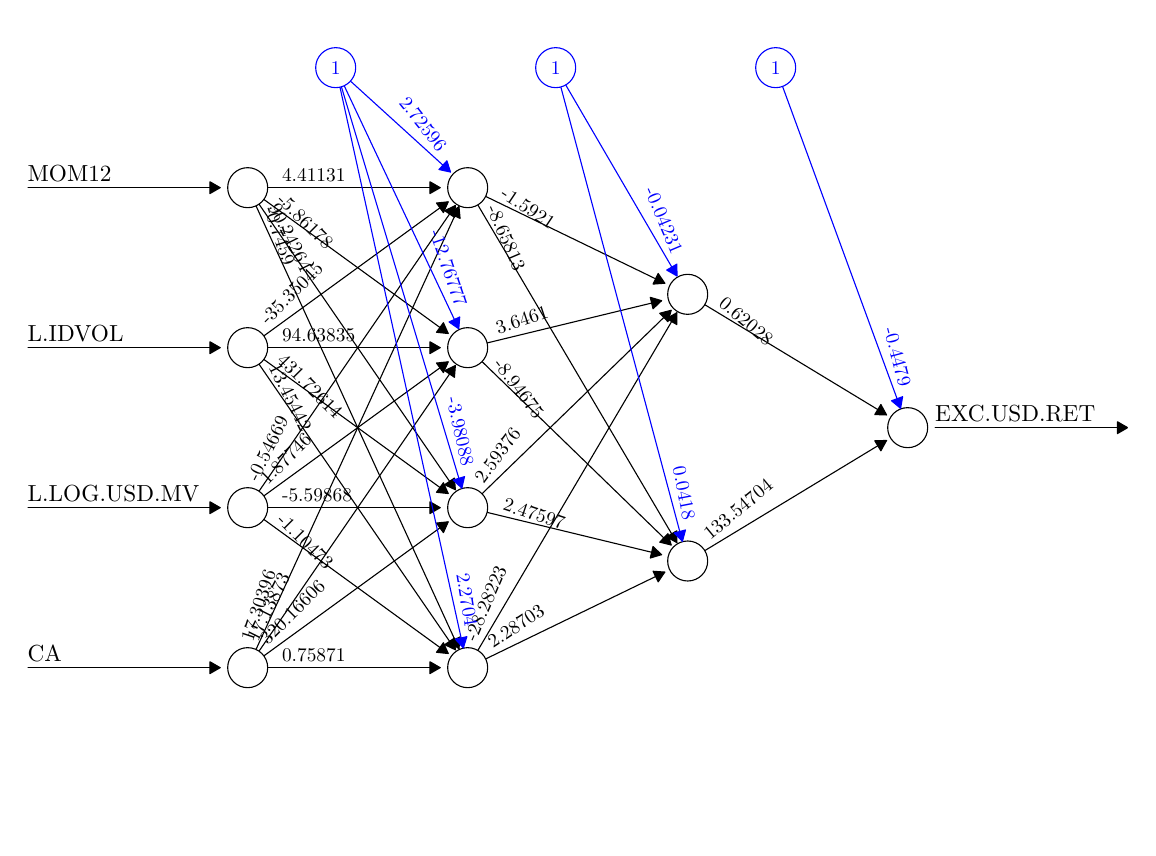
\begin{tikzpicture}[x=1pt,y=1pt]
\definecolor{fillColor}{RGB}{255,255,255}
\path[use as bounding box,fill=fillColor,fill opacity=0.00] (0,0) rectangle (397.48,289.08);
\begin{scope}
\path[clip] (  0.00,  0.00) rectangle (397.48,289.08);
\definecolor{drawColor}{RGB}{0,0,0}

\path[draw=drawColor,line width= 0.4pt,line join=round,line cap=round] ( 79.50, 57.82) --
	(149.06, 57.82);
\definecolor{fillColor}{RGB}{0,0,0}

\path[draw=drawColor,line width= 0.4pt,line join=round,line cap=round,fill=fillColor] (145.36, 55.68) --
	(149.06, 57.82) --
	(145.36, 59.95) --
	cycle;

\node[text=drawColor,anchor=base west,inner sep=0pt, outer sep=0pt, scale=  0.70] at ( 91.92, 59.95) {0.75871};
\end{scope}
\begin{scope}
\path[clip] (  0.00,  0.00) rectangle (397.48,289.08);
\definecolor{drawColor}{RGB}{0,0,0}

\path[draw=drawColor,line width= 0.4pt,line join=round,line cap=round] ( 79.50, 57.82) --
	(151.97,110.52);
\definecolor{fillColor}{RGB}{0,0,0}

\path[draw=drawColor,line width= 0.4pt,line join=round,line cap=round,fill=fillColor] (150.23,106.62) --
	(151.97,110.52) --
	(147.72,110.07) --
	cycle;

\node[text=drawColor,rotate= 45.00,anchor=base west,inner sep=0pt, outer sep=0pt, scale=  0.70] at ( 86.77, 65.71) {320.16606};
\end{scope}
\begin{scope}
\path[clip] (  0.00,  0.00) rectangle (397.48,289.08);
\definecolor{drawColor}{RGB}{0,0,0}

\path[draw=drawColor,line width= 0.4pt,line join=round,line cap=round] ( 79.50, 57.82) --
	(154.55,166.98);
\definecolor{fillColor}{RGB}{0,0,0}

\path[draw=drawColor,line width= 0.4pt,line join=round,line cap=round,fill=fillColor] (154.21,162.73) --
	(154.55,166.98) --
	(150.70,165.15) --
	cycle;

\node[text=drawColor,rotate= 63.43,anchor=base west,inner sep=0pt, outer sep=0pt, scale=  0.70] at ( 83.14, 66.85) {17.13873};
\end{scope}
\begin{scope}
\path[clip] (  0.00,  0.00) rectangle (397.48,289.08);
\definecolor{drawColor}{RGB}{0,0,0}

\path[draw=drawColor,line width= 0.4pt,line join=round,line cap=round] ( 79.50, 57.82) --
	(155.85,224.41);
\definecolor{fillColor}{RGB}{0,0,0}

\path[draw=drawColor,line width= 0.4pt,line join=round,line cap=round,fill=fillColor] (156.25,220.16) --
	(155.85,224.41) --
	(152.37,221.94) --
	cycle;

\node[text=drawColor,rotate= 71.57,anchor=base west,inner sep=0pt, outer sep=0pt, scale=  0.70] at ( 81.40, 67.06) {17.30396};
\end{scope}
\begin{scope}
\path[clip] (  0.00,  0.00) rectangle (397.48,289.08);
\definecolor{drawColor}{RGB}{0,0,0}

\path[draw=drawColor,line width= 0.4pt,line join=round,line cap=round] ( -0.00, 57.82) --
	( 69.56, 57.82);
\definecolor{fillColor}{RGB}{0,0,0}

\path[draw=drawColor,line width= 0.4pt,line join=round,line cap=round,fill=fillColor] ( 65.86, 55.68) --
	( 69.56, 57.82) --
	( 65.86, 59.95) --
	cycle;

\node[text=drawColor,anchor=base west,inner sep=0pt, outer sep=0pt, scale=  0.84] at ( -0.00, 59.95) {CA};
\end{scope}
\begin{scope}
\path[clip] (  0.00,  0.00) rectangle (397.48,289.08);
\definecolor{drawColor}{RGB}{0,0,0}
\definecolor{fillColor}{RGB}{255,255,255}

\path[draw=drawColor,line width= 0.4pt,line join=round,line cap=round,fill=fillColor] ( 79.50, 57.82) circle (  7.23);

\path[draw=drawColor,line width= 0.4pt,line join=round,line cap=round] ( 79.50,115.63) --
	(151.97, 62.93);
\definecolor{fillColor}{RGB}{0,0,0}

\path[draw=drawColor,line width= 0.4pt,line join=round,line cap=round,fill=fillColor] (147.72, 63.37) --
	(151.97, 62.93) --
	(150.23, 66.83) --
	cycle;

\node[text=drawColor,rotate=-45.00,anchor=base west,inner sep=0pt, outer sep=0pt, scale=  0.70] at ( 89.79,110.75) {-1.10473};
\end{scope}
\begin{scope}
\path[clip] (  0.00,  0.00) rectangle (397.48,289.08);
\definecolor{drawColor}{RGB}{0,0,0}

\path[draw=drawColor,line width= 0.4pt,line join=round,line cap=round] ( 79.50,115.63) --
	(149.06,115.63);
\definecolor{fillColor}{RGB}{0,0,0}

\path[draw=drawColor,line width= 0.4pt,line join=round,line cap=round,fill=fillColor] (145.36,113.50) --
	(149.06,115.63) --
	(145.36,117.77) --
	cycle;

\node[text=drawColor,anchor=base west,inner sep=0pt, outer sep=0pt, scale=  0.70] at ( 91.92,117.77) {-5.59868};
\end{scope}
\begin{scope}
\path[clip] (  0.00,  0.00) rectangle (397.48,289.08);
\definecolor{drawColor}{RGB}{0,0,0}

\path[draw=drawColor,line width= 0.4pt,line join=round,line cap=round] ( 79.50,115.63) --
	(151.97,168.34);
\definecolor{fillColor}{RGB}{0,0,0}

\path[draw=drawColor,line width= 0.4pt,line join=round,line cap=round,fill=fillColor] (150.23,164.44) --
	(151.97,168.34) --
	(147.72,167.89) --
	cycle;

\node[text=drawColor,rotate= 45.00,anchor=base west,inner sep=0pt, outer sep=0pt, scale=  0.70] at ( 86.77,123.53) {1.87746};
\end{scope}
\begin{scope}
\path[clip] (  0.00,  0.00) rectangle (397.48,289.08);
\definecolor{drawColor}{RGB}{0,0,0}

\path[draw=drawColor,line width= 0.4pt,line join=round,line cap=round] ( 79.50,115.63) --
	(154.55,224.80);
\definecolor{fillColor}{RGB}{0,0,0}

\path[draw=drawColor,line width= 0.4pt,line join=round,line cap=round,fill=fillColor] (154.21,220.55) --
	(154.55,224.80) --
	(150.70,222.96) --
	cycle;

\node[text=drawColor,rotate= 63.43,anchor=base west,inner sep=0pt, outer sep=0pt, scale=  0.70] at ( 83.14,124.67) {-0.54669};
\end{scope}
\begin{scope}
\path[clip] (  0.00,  0.00) rectangle (397.48,289.08);
\definecolor{drawColor}{RGB}{0,0,0}

\path[draw=drawColor,line width= 0.4pt,line join=round,line cap=round] ( -0.00,115.63) --
	( 69.56,115.63);
\definecolor{fillColor}{RGB}{0,0,0}

\path[draw=drawColor,line width= 0.4pt,line join=round,line cap=round,fill=fillColor] ( 65.86,113.50) --
	( 69.56,115.63) --
	( 65.86,117.77) --
	cycle;

\node[text=drawColor,anchor=base west,inner sep=0pt, outer sep=0pt, scale=  0.84] at ( -0.00,117.77) {L.LOG.USD.MV};
\end{scope}
\begin{scope}
\path[clip] (  0.00,  0.00) rectangle (397.48,289.08);
\definecolor{drawColor}{RGB}{0,0,0}
\definecolor{fillColor}{RGB}{255,255,255}

\path[draw=drawColor,line width= 0.4pt,line join=round,line cap=round,fill=fillColor] ( 79.50,115.63) circle (  7.23);

\path[draw=drawColor,line width= 0.4pt,line join=round,line cap=round] ( 79.50,173.45) --
	(154.55, 64.28);
\definecolor{fillColor}{RGB}{0,0,0}

\path[draw=drawColor,line width= 0.4pt,line join=round,line cap=round,fill=fillColor] (150.70, 66.12) --
	(154.55, 64.28) --
	(154.21, 68.53) --
	cycle;

\node[text=drawColor,rotate=-63.43,anchor=base west,inner sep=0pt, outer sep=0pt, scale=  0.70] at ( 86.96,166.32) {13.45442};
\end{scope}
\begin{scope}
\path[clip] (  0.00,  0.00) rectangle (397.48,289.08);
\definecolor{drawColor}{RGB}{0,0,0}

\path[draw=drawColor,line width= 0.4pt,line join=round,line cap=round] ( 79.50,173.45) --
	(151.97,120.74);
\definecolor{fillColor}{RGB}{0,0,0}

\path[draw=drawColor,line width= 0.4pt,line join=round,line cap=round,fill=fillColor] (147.72,121.19) --
	(151.97,120.74) --
	(150.23,124.64) --
	cycle;

\node[text=drawColor,rotate=-45.00,anchor=base west,inner sep=0pt, outer sep=0pt, scale=  0.70] at ( 89.79,168.57) {431.72614};
\end{scope}
\begin{scope}
\path[clip] (  0.00,  0.00) rectangle (397.48,289.08);
\definecolor{drawColor}{RGB}{0,0,0}

\path[draw=drawColor,line width= 0.4pt,line join=round,line cap=round] ( 79.50,173.45) --
	(149.06,173.45);
\definecolor{fillColor}{RGB}{0,0,0}

\path[draw=drawColor,line width= 0.4pt,line join=round,line cap=round,fill=fillColor] (145.36,171.31) --
	(149.06,173.45) --
	(145.36,175.58) --
	cycle;

\node[text=drawColor,anchor=base west,inner sep=0pt, outer sep=0pt, scale=  0.70] at ( 91.92,175.58) {94.63835};
\end{scope}
\begin{scope}
\path[clip] (  0.00,  0.00) rectangle (397.48,289.08);
\definecolor{drawColor}{RGB}{0,0,0}

\path[draw=drawColor,line width= 0.4pt,line join=round,line cap=round] ( 79.50,173.45) --
	(151.97,226.15);
\definecolor{fillColor}{RGB}{0,0,0}

\path[draw=drawColor,line width= 0.4pt,line join=round,line cap=round,fill=fillColor] (150.23,222.25) --
	(151.97,226.15) --
	(147.72,225.71) --
	cycle;

\node[text=drawColor,rotate= 45.00,anchor=base west,inner sep=0pt, outer sep=0pt, scale=  0.70] at ( 86.77,181.34) {-35.35045};
\end{scope}
\begin{scope}
\path[clip] (  0.00,  0.00) rectangle (397.48,289.08);
\definecolor{drawColor}{RGB}{0,0,0}

\path[draw=drawColor,line width= 0.4pt,line join=round,line cap=round] ( -0.00,173.45) --
	( 69.56,173.45);
\definecolor{fillColor}{RGB}{0,0,0}

\path[draw=drawColor,line width= 0.4pt,line join=round,line cap=round,fill=fillColor] ( 65.86,171.31) --
	( 69.56,173.45) --
	( 65.86,175.58) --
	cycle;

\node[text=drawColor,anchor=base west,inner sep=0pt, outer sep=0pt, scale=  0.84] at ( -0.00,175.58) {L.IDVOL};
\end{scope}
\begin{scope}
\path[clip] (  0.00,  0.00) rectangle (397.48,289.08);
\definecolor{drawColor}{RGB}{0,0,0}
\definecolor{fillColor}{RGB}{255,255,255}

\path[draw=drawColor,line width= 0.4pt,line join=round,line cap=round,fill=fillColor] ( 79.50,173.45) circle (  7.23);

\path[draw=drawColor,line width= 0.4pt,line join=round,line cap=round] ( 79.50,231.26) --
	(155.85, 64.67);
\definecolor{fillColor}{RGB}{0,0,0}

\path[draw=drawColor,line width= 0.4pt,line join=round,line cap=round,fill=fillColor] (152.37, 67.14) --
	(155.85, 64.67) --
	(156.25, 68.92) --
	cycle;

\node[text=drawColor,rotate=-71.57,anchor=base west,inner sep=0pt, outer sep=0pt, scale=  0.70] at ( 85.45,223.37) {-0.7459};
\end{scope}
\begin{scope}
\path[clip] (  0.00,  0.00) rectangle (397.48,289.08);
\definecolor{drawColor}{RGB}{0,0,0}

\path[draw=drawColor,line width= 0.4pt,line join=round,line cap=round] ( 79.50,231.26) --
	(154.55,122.10);
\definecolor{fillColor}{RGB}{0,0,0}

\path[draw=drawColor,line width= 0.4pt,line join=round,line cap=round,fill=fillColor] (150.70,123.93) --
	(154.55,122.10) --
	(154.21,126.35) --
	cycle;

\node[text=drawColor,rotate=-63.43,anchor=base west,inner sep=0pt, outer sep=0pt, scale=  0.70] at ( 86.96,224.14) {90.24264};
\end{scope}
\begin{scope}
\path[clip] (  0.00,  0.00) rectangle (397.48,289.08);
\definecolor{drawColor}{RGB}{0,0,0}

\path[draw=drawColor,line width= 0.4pt,line join=round,line cap=round] ( 79.50,231.26) --
	(151.97,178.56);
\definecolor{fillColor}{RGB}{0,0,0}

\path[draw=drawColor,line width= 0.4pt,line join=round,line cap=round,fill=fillColor] (147.72,179.01) --
	(151.97,178.56) --
	(150.23,182.46) --
	cycle;

\node[text=drawColor,rotate=-45.00,anchor=base west,inner sep=0pt, outer sep=0pt, scale=  0.70] at ( 89.79,226.39) {-5.86178};
\end{scope}
\begin{scope}
\path[clip] (  0.00,  0.00) rectangle (397.48,289.08);
\definecolor{drawColor}{RGB}{0,0,0}

\path[draw=drawColor,line width= 0.4pt,line join=round,line cap=round] ( 79.50,231.26) --
	(149.06,231.26);
\definecolor{fillColor}{RGB}{0,0,0}

\path[draw=drawColor,line width= 0.4pt,line join=round,line cap=round,fill=fillColor] (145.36,229.13) --
	(149.06,231.26) --
	(145.36,233.40) --
	cycle;

\node[text=drawColor,anchor=base west,inner sep=0pt, outer sep=0pt, scale=  0.70] at ( 91.92,233.40) {4.41131};
\end{scope}
\begin{scope}
\path[clip] (  0.00,  0.00) rectangle (397.48,289.08);
\definecolor{drawColor}{RGB}{0,0,0}

\path[draw=drawColor,line width= 0.4pt,line join=round,line cap=round] ( -0.00,231.26) --
	( 69.56,231.26);
\definecolor{fillColor}{RGB}{0,0,0}

\path[draw=drawColor,line width= 0.4pt,line join=round,line cap=round,fill=fillColor] ( 65.86,229.13) --
	( 69.56,231.26) --
	( 65.86,233.40) --
	cycle;

\node[text=drawColor,anchor=base west,inner sep=0pt, outer sep=0pt, scale=  0.84] at ( -0.00,233.40) {MOM12};
\end{scope}
\begin{scope}
\path[clip] (  0.00,  0.00) rectangle (397.48,289.08);
\definecolor{drawColor}{RGB}{0,0,0}
\definecolor{fillColor}{RGB}{255,255,255}

\path[draw=drawColor,line width= 0.4pt,line join=round,line cap=round,fill=fillColor] ( 79.50,231.26) circle (  7.23);

\path[draw=drawColor,line width= 0.4pt,line join=round,line cap=round] (158.99, 57.82) --
	(230.22, 92.35);
\definecolor{fillColor}{RGB}{0,0,0}

\path[draw=drawColor,line width= 0.4pt,line join=round,line cap=round,fill=fillColor] (227.83, 88.82) --
	(230.22, 92.35) --
	(225.97, 92.66) --
	cycle;

\node[text=drawColor,rotate= 33.69,anchor=base west,inner sep=0pt, outer sep=0pt, scale=  0.70] at (168.15, 64.60) {2.28703};
\end{scope}
\begin{scope}
\path[clip] (  0.00,  0.00) rectangle (397.48,289.08);
\definecolor{drawColor}{RGB}{0,0,0}

\path[draw=drawColor,line width= 0.4pt,line join=round,line cap=round] (158.99, 57.82) --
	(234.58,186.08);
\definecolor{fillColor}{RGB}{0,0,0}

\path[draw=drawColor,line width= 0.4pt,line join=round,line cap=round,fill=fillColor] (234.54,181.81) --
	(234.58,186.08) --
	(230.86,183.98) --
	cycle;

\node[text=drawColor,rotate= 66.80,anchor=base west,inner sep=0pt, outer sep=0pt, scale=  0.70] at (161.93, 66.96) {-28.28223};
\end{scope}
\begin{scope}
\path[clip] (  0.00,  0.00) rectangle (397.48,289.08);
\definecolor{drawColor}{RGB}{0,0,0}
\definecolor{fillColor}{RGB}{255,255,255}

\path[draw=drawColor,line width= 0.4pt,line join=round,line cap=round,fill=fillColor] (158.99, 57.82) circle (  7.23);

\path[draw=drawColor,line width= 0.4pt,line join=round,line cap=round] (158.99,115.63) --
	(229.06, 98.65);
\definecolor{fillColor}{RGB}{0,0,0}

\path[draw=drawColor,line width= 0.4pt,line join=round,line cap=round,fill=fillColor] (224.97, 97.44) --
	(229.06, 98.65) --
	(225.97,101.59) --
	cycle;

\node[text=drawColor,rotate=-18.43,anchor=base west,inner sep=0pt, outer sep=0pt, scale=  0.70] at (171.45,114.80) {2.47597};
\end{scope}
\begin{scope}
\path[clip] (  0.00,  0.00) rectangle (397.48,289.08);
\definecolor{drawColor}{RGB}{0,0,0}

\path[draw=drawColor,line width= 0.4pt,line join=round,line cap=round] (158.99,115.63) --
	(232.53,186.94);
\definecolor{fillColor}{RGB}{0,0,0}

\path[draw=drawColor,line width= 0.4pt,line join=round,line cap=round,fill=fillColor] (231.36,182.83) --
	(232.53,186.94) --
	(228.39,185.90) --
	cycle;

\node[text=drawColor,rotate= 53.13,anchor=base west,inner sep=0pt, outer sep=0pt, scale=  0.70] at (164.74,124.14) {2.59376};
\end{scope}
\begin{scope}
\path[clip] (  0.00,  0.00) rectangle (397.48,289.08);
\definecolor{drawColor}{RGB}{0,0,0}
\definecolor{fillColor}{RGB}{255,255,255}

\path[draw=drawColor,line width= 0.4pt,line join=round,line cap=round,fill=fillColor] (158.99,115.63) circle (  7.23);

\path[draw=drawColor,line width= 0.4pt,line join=round,line cap=round] (158.99,173.45) --
	(232.53,102.14);
\definecolor{fillColor}{RGB}{0,0,0}

\path[draw=drawColor,line width= 0.4pt,line join=round,line cap=round,fill=fillColor] (228.39,103.18) --
	(232.53,102.14) --
	(231.36,106.25) --
	cycle;

\node[text=drawColor,rotate=-53.13,anchor=base west,inner sep=0pt, outer sep=0pt, scale=  0.70] at (168.15,167.50) {-8.94675};
\end{scope}
\begin{scope}
\path[clip] (  0.00,  0.00) rectangle (397.48,289.08);
\definecolor{drawColor}{RGB}{0,0,0}

\path[draw=drawColor,line width= 0.4pt,line join=round,line cap=round] (158.99,173.45) --
	(229.06,190.43);
\definecolor{fillColor}{RGB}{0,0,0}

\path[draw=drawColor,line width= 0.4pt,line join=round,line cap=round,fill=fillColor] (225.97,187.49) --
	(229.06,190.43) --
	(224.97,191.64) --
	cycle;

\node[text=drawColor,rotate= 18.43,anchor=base west,inner sep=0pt, outer sep=0pt, scale=  0.70] at (170.10,178.33) {3.6461};
\end{scope}
\begin{scope}
\path[clip] (  0.00,  0.00) rectangle (397.48,289.08);
\definecolor{drawColor}{RGB}{0,0,0}
\definecolor{fillColor}{RGB}{255,255,255}

\path[draw=drawColor,line width= 0.4pt,line join=round,line cap=round,fill=fillColor] (158.99,173.45) circle (  7.23);

\path[draw=drawColor,line width= 0.4pt,line join=round,line cap=round] (158.99,231.26) --
	(234.58,103.00);
\definecolor{fillColor}{RGB}{0,0,0}

\path[draw=drawColor,line width= 0.4pt,line join=round,line cap=round,fill=fillColor] (230.86,105.10) --
	(234.58,103.00) --
	(234.54,107.27) --
	cycle;

\node[text=drawColor,rotate=-66.80,anchor=base west,inner sep=0pt, outer sep=0pt, scale=  0.70] at (165.85,223.80) {-8.65813};
\end{scope}
\begin{scope}
\path[clip] (  0.00,  0.00) rectangle (397.48,289.08);
\definecolor{drawColor}{RGB}{0,0,0}

\path[draw=drawColor,line width= 0.4pt,line join=round,line cap=round] (158.99,231.26) --
	(230.22,196.73);
\definecolor{fillColor}{RGB}{0,0,0}

\path[draw=drawColor,line width= 0.4pt,line join=round,line cap=round,fill=fillColor] (225.97,196.42) --
	(230.22,196.73) --
	(227.83,200.26) --
	cycle;

\node[text=drawColor,rotate=-33.69,anchor=base west,inner sep=0pt, outer sep=0pt, scale=  0.70] at (170.51,228.03) {-1.5921};
\end{scope}
\begin{scope}
\path[clip] (  0.00,  0.00) rectangle (397.48,289.08);
\definecolor{drawColor}{RGB}{0,0,0}
\definecolor{fillColor}{RGB}{255,255,255}

\path[draw=drawColor,line width= 0.4pt,line join=round,line cap=round,fill=fillColor] (158.99,231.26) circle (  7.23);

\path[draw=drawColor,line width= 0.4pt,line join=round,line cap=round] (238.49, 96.36) --
	(310.35,139.91);
\definecolor{fillColor}{RGB}{0,0,0}

\path[draw=drawColor,line width= 0.4pt,line join=round,line cap=round,fill=fillColor] (308.30,136.17) --
	(310.35,139.91) --
	(306.09,139.82) --
	cycle;

\node[text=drawColor,rotate= 39.81,anchor=base west,inner sep=0pt, outer sep=0pt, scale=  0.70] at (246.67,103.78) {133.54704};
\end{scope}
\begin{scope}
\path[clip] (  0.00,  0.00) rectangle (397.48,289.08);
\definecolor{drawColor}{RGB}{0,0,0}
\definecolor{fillColor}{RGB}{255,255,255}

\path[draw=drawColor,line width= 0.4pt,line join=round,line cap=round,fill=fillColor] (238.49, 96.36) circle (  7.23);

\path[draw=drawColor,line width= 0.4pt,line join=round,line cap=round] (238.49,192.72) --
	(310.35,149.17);
\definecolor{fillColor}{RGB}{0,0,0}

\path[draw=drawColor,line width= 0.4pt,line join=round,line cap=round,fill=fillColor] (306.09,149.26) --
	(310.35,149.17) --
	(308.30,152.91) --
	cycle;

\node[text=drawColor,rotate=-39.81,anchor=base west,inner sep=0pt, outer sep=0pt, scale=  0.70] at (249.40,188.58) {0.62028};
\end{scope}
\begin{scope}
\path[clip] (  0.00,  0.00) rectangle (397.48,289.08);
\definecolor{drawColor}{RGB}{0,0,0}
\definecolor{fillColor}{RGB}{255,255,255}

\path[draw=drawColor,line width= 0.4pt,line join=round,line cap=round,fill=fillColor] (238.49,192.72) circle (  7.23);

\path[draw=drawColor,line width= 0.4pt,line join=round,line cap=round] (327.93,144.54) --
	(397.48,144.54);
\definecolor{fillColor}{RGB}{0,0,0}

\path[draw=drawColor,line width= 0.4pt,line join=round,line cap=round,fill=fillColor] (393.79,142.41) --
	(397.48,144.54) --
	(393.79,146.67) --
	cycle;

\node[text=drawColor,anchor=base west,inner sep=0pt, outer sep=0pt, scale=  0.84] at (327.93,146.67) {EXC.USD.RET};
\end{scope}
\begin{scope}
\path[clip] (  0.00,  0.00) rectangle (397.48,289.08);
\definecolor{drawColor}{RGB}{0,0,0}
\definecolor{fillColor}{RGB}{255,255,255}

\path[draw=drawColor,line width= 0.4pt,line join=round,line cap=round,fill=fillColor] (317.99,144.54) circle (  7.23);
\definecolor{drawColor}{RGB}{0,0,255}

\path[draw=drawColor,line width= 0.4pt,line join=round,line cap=round] (111.30,274.63) --
	(157.42, 64.95);
\definecolor{fillColor}{RGB}{0,0,255}

\path[draw=drawColor,line width= 0.4pt,line join=round,line cap=round,fill=fillColor] (154.55, 68.10) --
	(157.42, 64.95) --
	(158.71, 69.02) --
	cycle;

\node[text=drawColor,rotate=-80.91,anchor=base east,inner sep=0pt, outer sep=0pt, scale=  0.70] at (157.96, 72.43) {2.2704};
\end{scope}
\begin{scope}
\path[clip] (  0.00,  0.00) rectangle (397.48,289.08);
\definecolor{drawColor}{RGB}{0,0,255}

\path[draw=drawColor,line width= 0.4pt,line join=round,line cap=round] (111.30,274.63) --
	(156.88,122.69);
\definecolor{fillColor}{RGB}{0,0,255}

\path[draw=drawColor,line width= 0.4pt,line join=round,line cap=round,fill=fillColor] (153.77,125.62) --
	(156.88,122.69) --
	(157.86,126.85) --
	cycle;

\node[text=drawColor,rotate=-77.69,anchor=base east,inner sep=0pt, outer sep=0pt, scale=  0.70] at (156.84,130.21) {-3.98088};
\end{scope}
\begin{scope}
\path[clip] (  0.00,  0.00) rectangle (397.48,289.08);
\definecolor{drawColor}{RGB}{0,0,255}

\path[draw=drawColor,line width= 0.4pt,line join=round,line cap=round] (111.30,274.63) --
	(155.77,180.28);
\definecolor{fillColor}{RGB}{0,0,255}

\path[draw=drawColor,line width= 0.4pt,line join=round,line cap=round,fill=fillColor] (152.26,182.72) --
	(155.77,180.28) --
	(156.13,184.54) --
	cycle;

\node[text=drawColor,rotate=-71.08,anchor=base east,inner sep=0pt, outer sep=0pt, scale=  0.70] at (154.57,187.81) {-12.76777};
\end{scope}
\begin{scope}
\path[clip] (  0.00,  0.00) rectangle (397.48,289.08);
\definecolor{drawColor}{RGB}{0,0,255}

\path[draw=drawColor,line width= 0.4pt,line join=round,line cap=round] (111.30,274.63) --
	(152.79,236.91);
\definecolor{fillColor}{RGB}{0,0,255}

\path[draw=drawColor,line width= 0.4pt,line join=round,line cap=round,fill=fillColor] (148.62,237.81) --
	(152.79,236.91) --
	(151.49,240.97) --
	cycle;

\node[text=drawColor,rotate=-51.34,anchor=base east,inner sep=0pt, outer sep=0pt, scale=  0.70] at (148.24,243.88) {2.72596};
\end{scope}
\begin{scope}
\path[clip] (  0.00,  0.00) rectangle (397.48,289.08);
\definecolor{drawColor}{RGB}{0,0,255}
\definecolor{fillColor}{RGB}{255,255,255}

\path[draw=drawColor,line width= 0.4pt,line join=round,line cap=round,fill=fillColor] (111.30,274.63) circle (  7.23);

\node[text=drawColor,anchor=base,inner sep=0pt, outer sep=0pt, scale=  0.70] at (111.30,272.22) {1};

\path[draw=drawColor,line width= 0.4pt,line join=round,line cap=round] (190.79,274.63) --
	(236.59,103.45);
\definecolor{fillColor}{RGB}{0,0,255}

\path[draw=drawColor,line width= 0.4pt,line join=round,line cap=round,fill=fillColor] (233.58,106.47) --
	(236.59,103.45) --
	(237.70,107.58) --
	cycle;

\node[text=drawColor,rotate=-78.99,anchor=base east,inner sep=0pt, outer sep=0pt, scale=  0.70] at (236.79,110.96) {0.0418};
\end{scope}
\begin{scope}
\path[clip] (  0.00,  0.00) rectangle (397.48,289.08);
\definecolor{drawColor}{RGB}{0,0,255}

\path[draw=drawColor,line width= 0.4pt,line join=round,line cap=round] (190.79,274.63) --
	(234.62,199.37);
\definecolor{fillColor}{RGB}{0,0,255}

\path[draw=drawColor,line width= 0.4pt,line join=round,line cap=round,fill=fillColor] (230.91,201.49) --
	(234.62,199.37) --
	(234.60,203.64) --
	cycle;

\node[text=drawColor,rotate=-67.05,anchor=base east,inner sep=0pt, outer sep=0pt, scale=  0.70] at (232.71,206.86) {-0.04231};
\end{scope}
\begin{scope}
\path[clip] (  0.00,  0.00) rectangle (397.48,289.08);
\definecolor{drawColor}{RGB}{0,0,255}
\definecolor{fillColor}{RGB}{255,255,255}

\path[draw=drawColor,line width= 0.4pt,line join=round,line cap=round,fill=fillColor] (190.79,274.63) circle (  7.23);

\node[text=drawColor,anchor=base,inner sep=0pt, outer sep=0pt, scale=  0.70] at (190.79,272.22) {1};

\path[draw=drawColor,line width= 0.4pt,line join=round,line cap=round] (270.29,274.63) --
	(315.43,151.52);
\definecolor{fillColor}{RGB}{0,0,255}

\path[draw=drawColor,line width= 0.4pt,line join=round,line cap=round,fill=fillColor] (312.15,154.26) --
	(315.43,151.52) --
	(316.16,155.73) --
	cycle;

\node[text=drawColor,rotate=-75.07,anchor=base east,inner sep=0pt, outer sep=0pt, scale=  0.70] at (314.93,159.06) {-0.4479};
\end{scope}
\begin{scope}
\path[clip] (  0.00,  0.00) rectangle (397.48,289.08);
\definecolor{drawColor}{RGB}{0,0,255}
\definecolor{fillColor}{RGB}{255,255,255}

\path[draw=drawColor,line width= 0.4pt,line join=round,line cap=round,fill=fillColor] (270.29,274.63) circle (  7.23);

\node[text=drawColor,anchor=base,inner sep=0pt, outer sep=0pt, scale=  0.70] at (270.29,272.22) {1};
\end{scope}
\end{tikzpicture}

\label{plot:NN}
\end{figure}

Idea of the neural network is that each neuron, using weights and biases terms, aggregates information from previous layer and subsequently feeds the information to the activations function. Neural network model used in this study is fully connected, meaning that each neuron is connected to all neurons in previous layer. Output of the activation function will be the input for the next layer. Neural network model is trained by optimizing these weights and biases terms. There exists many options for the activation function, which is again one choice user has to make. Activation function used in this study is rectified linear unit \par

\begin{equation}
\label{ReLU}
ReLU(x) = max(0, x)
\end{equation}

Since model is trained for a regression task final neuron in the output layer has different activation function than the neurons in the hidden layers. Activation function for the output neuron is linear function. \par

As mentioned neural networks include numerous hyperparameters that can be optimized during the training of the model. Training neural network is computationally demanding. Due to limited computing capacity hyperparameters are not optimized in this study, but predefined values are used. Hyperparameters and their values are presented in table \ref{table:Hyperparameters}. Additionally, to further limit the computational demand and simultaneously avoid overfitting early stopping algorithm is applied. Early stopping is implemented so that training of the model is terminated after five epochs where the loss function value does not reduce for validation set. Instead of inserting whole dataset to the model at once data is inserted to the model in smaller subsamples so called batches. Epoch on the other hand measures how many times the whole dataset is run through the model. \par

Neural networks learn by adjusting weights to the direction of gradient. This is done in repetitive iterations. In each iteration size of the change is defined by hyperparameter called learning rate. Since learning rate is a hyperparameter it needs an input from the user. It can also be optimized. Setting correct learning rate is crucial, since too big learning rate might prevent algorithm from converging to optimal solution, but too small learning rate makes converging slow. For above described reasons learning rate is not optimized in this study, but using learning rate scheduler it is adjusted during the training of the model. In order to ensure efficient training learning rate is set 0.01 in the beginning of the training and after ten epochs learning rate will be multiplied by 0.9. \par

Neural networks are also sensitive to the weight initialization, where the initial weights are set which the model starts to optimize. Depending on the initialization of the weights neural networks can converge to different results. To reduce model variance caused by this, an ensemble method is applied. Ensemble is implemented by training five separate models with different initial weights. Final prediction will be then average of the predictions of the five models. \par

\subsection{Prediction performance evaluation}\label{PredictionPerformanceEvaluation}

This study will evaluate machine learning methods from two perspectives. First perspective that is evaluated is the profitability of the methods. Profitability is estimated via portfolio construction following Lewellen \citeyear{Lewellen2015}. First expected returns are derived from each model. This process is introduced in more detail in following subsections. After obtaining the expected returns, each month all stocks are distributed to ten portfolios based on the magnitude of the expected return. Allocation is univariate and does not consider other variables than the expected return of the stock for the next month. Even though models are trained only once a year, expected returns are re-calculated every month as the most recent available data is inserted to the model. Therefore, also the portfolio allocation is repeated monthly. Each month all stocks are allocated to one of the ten expected return portfolio, but to avoid result to be mainly driven by small stocks approach from Hanauer and Kalsbach is applied \citeyear{HANAUER2023}  and the breakpoints for the allocation are calculated only from the large market value stocks. Large market value stocks are the biggest stocks that account for 97\% of the aggregated total market value of respective month. \par

In addition to the ten expected return portfolios, for each method zero investment portfolio is formed. Zero investment or long-short portfolio is simply the spread between return of the highest expected return portfolio and return of the lowest expected return portfolio. Both value and equal weighted returns will be reported for each portfolio. Performance of the machine learning portfolios is backtested and evaluated in multiple ways. For all expected return portfolios historical realized mean returns are reported together with Sharpe ratios. For long-short portfolios also maximum drawdown and maximum 1 month loss will be reported. Maximum 1 month loss is simply the largest negative monthly return of each portfolio. Maximum drawdown is define as \par

\begin{equation}
\label{eq:maxDD}
MaxDD = \max\limits_{0\leq t_1\leq t_2\leq T} (Y_{t_1} - Y_{t_2})
\end{equation}

where $Y_t$ stands for cumulative return from the beginning of the period until date $t$. Turnover will be calculated only for long side of the long-short portfolios. In order to examine risk adjusted returns long-short portfolio returns will be regressed against Fama-French \citeyear{FAMA20151} six factor model factors \footnotemark. From this regression alphas, which can interpret as the excess return that the models are able to generate that cannot be explained by the loadings in the six risk factors. Also $t$-statistics for the alphas and $R^2$ values are reported. Regression formula for risk adjusted performance \par

\begin{equation}
\label{eq:FFRegFormula}
\begin{split}
\hat r_{i, t} = 	& \ \alpha+ \beta_{1} \ RMRF{t} + \beta_{2} + \ SMB_{t} + \beta_{3} \ HML_{t} + \\
		&  \beta_{4} \ CMA_{t} +  \beta_{5} \ RMW_{t} + \beta_{6} \ MOM_{t} + \epsilon_{t}
\end{split}
\end{equation}

where $RMRF$ is the excess market return, $SMB$ is the spread in the return between small market value stocks and large market value stocks, $HML$ is the spread in the return between high book-to-market value stocks and low book-to-market value stocks, $CMA$ is the spread in the return between conservatively investing stocks and aggressively investing stocks, $RMW$ is the spread in the return between stocks with robust profitability and stocks with weak profitability and $MOM$ is the between returns of stocks that had highest return in period $t-1$ and the stocks that had lowest return in period $t-1$. Factors are constructed from the same dataset as machine learning portfolios, except that the micro-cap stocks are not excluded. Construction of these factors is described in more detail in Appendix. \par

\footnotetext{Fama and French \citeyear{FAMA20151} introduced the five factor model. Factors used to regress machine learning portfolio returns include five factor model factors and momentum factor from Carhart \citeyear{Carhart1997}.}

Machine learning models are also evaluated based on their prediction accuracy. Prediction accuracy will be evaluated using out-of-sample $R^{2}_{oos}$ and Diebold-Mariano tests. Two out-of-sample $R^{2}$ figures are presented. Traditional out-of-sample $R^{2}$ uses historical mean  return as the benchmark estimation. Traditional out-of-sample $R^{2}$ is defined as \par

\begin{equation}
\label{eq:r2Trad}
R^{2}_{oos \ Trad.} = 1 - \frac{\sum^T_{t=1} \sum^N_{i=1} (r_{i, t} - \hat r_{i, t})^2}{ \sum^T_{t=1} \sum^N_{i=1} (r_{i, t} - \overline{r}_{i, t} )^2}
\end{equation}

where $r_{i, t}$ is the realized return of stock $i$ in month $t$, $\hat r_{i, t}$ is the predicted return of the same stock for month $i$ and $\overline{r}_{i, t}$ is the historical mean return of the same stock excluding month $i$. Nevertheless, Gu et al. \citeyear{guetal} argue that the historical mean return is so noisy estimator that it underperforms compared to static estimation of zero and therefore artificially improves the out-of-sample $R^{2}$. Instead they propose alternative out-of-sample $R^{2}$ measure where the squared sum of returns in denominator is not demeaned. \par

\begin{equation}
\label{eq:r2}
R^{2}_{oos} = 1 - \frac{\sum^T_{t=1} \sum^N_{i=1} (r_{i, t} - \hat r_{i, t})^2}{ \sum^T_{t=1} \sum^N_{i=1} r^2_{i, t}}
\end{equation}

$R^2$ presents the prediction accuracy as a single figure, whereas Diebold-Mariano allows for pairwise comparison of different models. Diebold-Mariano value is calculated as \par

\begin{equation}
\label{eq:Diebold-Mariano}
\begin{split}
 d_{12, t} 			& = \ \frac{1}{N_{t}}  \sum^N_{i=1}((r_{i, t} - \hat r_{i, t, 1})^2 - (r_{i, t} - \hat r_{i, t, 2})^2) \\
\overline{d}_{12} 	& = \ \frac{1}{T} \sum^T_{t=1} d_{12, t} \\
DM_{12} 			& = \ \frac{\overline{d}_{12}}{\hat \sigma_{d_{12}}} \\
\end{split}
\end{equation}

where $\hat r_{i, t, 1}$ is the return prediction of first model for company $i$ at time $t$ and $\hat r_{i, t, 1}$ is the return prediction of the second model  for company $i$ at time $t$. $N_t$ is number of observations in prediction period $t$. Therefore, $d_{12, t}$ is a time series of differences in average squared prediction errors between model $1$ and model $2$. $\overline{d}_{12}$ is the mean of $d_{12, t}$ and $\hat \sigma_{d_{12}}$ is the Newey and West (source) standard error of $d_{12, t}$. Diebold-Mariano test allows us to estimate statistical significance of the prediction accuracy of two models. Under assumption that the there does not exists difference in prediction accuracy between models Diebold-Mariano test statistic follows norma distribution with mean of $0$ and standard deviation of $1$, $DM \sim \mathcal{N}(0,\, 1)$. The significance of the difference is reported both for traditional $5\%$ level as well as for 3-way comparisons with Bonferroni adjustment. \par

In the spirit of Lewellen \citeyear{Lewellen2015} expected returns are also estimated by regressing realized returns with the expected returns. This regression follows \par

\begin{equation}
\label{eq:realizedRegression}
r_{i, t} = \alpha + \beta_1 \hat r_{i, t}
\end{equation}

where $r_{i, t}$ is the realized return of company $i$ at time $t$ and $\hat r_{i, t}$ is the expected return of corresponding model for company $i$ at time $t$. For these regressions betas, $t$-statistics for betas and $R^2$ values will be reported. Ideally the beta coefficient or the slope for the predicted return should be 1 and highly significant. Magnitude of the beta coefficients can provide information of possible over or undershooting of the models. \par

\subsection{Variable importance} \label{VariableImportance}

One challenge in dealing with various statistical methods is that they lack common metrics for explanatory inference. Many of the models have metrics for variable importance, but comparability of these metrics can be questioned. Therefore, approach of Gu et al. \citeyear{guetal} is implemented to define variable importance metrics for model applied in this study. Approach consists of following steps. First one variable at a time is set to zero. Then the reduced model is retrained and new predicted returns are derived using the reduced model. Process of training and predicting returns is identical to the reduced model as for the full model. After obtaining the predicted returns from reduced model, out-of-sample $R^2$ values are calculated for these returns. Then change compared to out-of-sample $R^2$ of full model is calculated. Finally, to obtain relative variable importance metric sum of changes in out-of-sample $R^2$s is normalized to one within model. Same process is applied to each variable and all models. \par

\subsection{Sample splitting} \label{SampleSplitting}

It is common while training machine learning models to split the data to three sets. Training set will be used as the name suggest to train the model. In case machine learning model includes hyperparameters these can be optimized with validation set. Finally the true out-of-sample predictions can be performed for testing data. Because we want to mimic situation and information set of an investor we have to take into a consideration time series nature of the data. \par

In stock return prediction literature it is common to split the data as described above, but considering the chronological order. For example Fieberg et al. \citeyear{Fieberg} use rolling 10 year rolling scheme where they first train model using the first seven years of the data and then optimize hyperparameters using last three years of the rolling window. Finally they train the model with optimal hyperparameter initalization with whole ten year window to predict returns for the next year. Gu et al. \citeyear{guetal} use slightly different approach. Instead of using rolling window they increase the training window size after each training period by one year. Common for these two approaches is that they both train the model only once a year. \par

\definecolor{Gray}{RGB}{160,160,160}
\definecolor{LightGray}{RGB}{191,191,191}
\begin{figure}[h]
\centering
\label{plot:SampleSplittingScheme}
\caption[Sample splitting scheme]{\textbf{Sample splitting}\\ Illustration sample splitting used in training of the machine learning models. Machine learning models are trained once a year and after each training model is used for next 12 months to predict the stock returns. Each year training period is extended by 12 months. Training period is further split into training data and validation data randomly allocating 80\% of the data to training set and 20\% of the data to the validation set. Validation set is used to optimize hyperparameters. Minimum length of the training period is 50 months.}
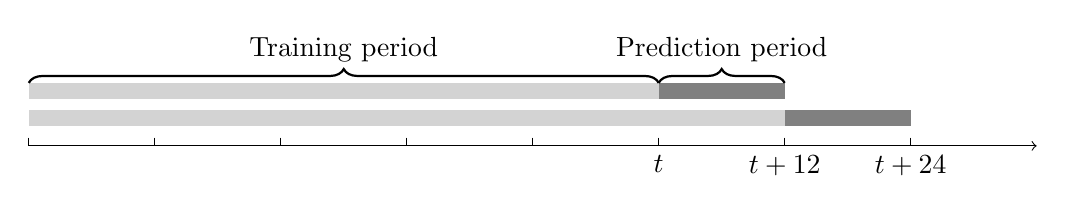
\begin{tikzpicture}
\draw[->] (0, 0) -- (12.8, 0);
\foreach \x in {0, 1.6,...,12.8}{
    \draw (\x cm, 3pt) -- (\x cm, 0pt);
} 
\fill[LightGray] (0, 0.8) rectangle (8, 0.6);
\fill[Gray] (8, 0.8) rectangle (9.6, 0.6);
\fill[LightGray] (0, 0.45) rectangle (9.6, 0.25);
\fill[Gray] (9.6, 0.45) rectangle (11.2, 0.25);

\draw [thick, decorate, decoration = {brace, amplitude = 5pt}] (0, 0.8)  -- +(8, 0) 
       node [black, midway, above = 4pt] {Training period};
\draw [thick, decorate, decoration = {brace, amplitude = 5pt}] (8, 0.8)  -- +(1.6, 0) 
       node [black, midway, above = 4pt] {Prediction period};
       
\node[anchor=north] at (8, 0) {$t$};
\node[anchor=north] at (9.6,0) {$t+12$};
\node[anchor=north] at (11.2, 0) {$t+24$};
\end{tikzpicture}
\label{plot:Turnover}
\end{figure}

The sample splitting scheme applied in this study is slightly different from above described ones. Above approaches use disjoint time periods to mimic the out-of-sample setting in the hyperparameter optimization. In this study training and validation set are separated from the testing data based on time. Approach is closer to approach of Gu et al. \citeyear{guetal} in a sense that training data window is increased each year. Nevertheless, the difference is that the data is distributed to training data and validation randomly instead of using the disjoint periods. Reason why this scheme is chosen is that we want to avoid the retraining of the model after the hyperparameter optimization which is necessary if the most recent data should be included to the model. Sample splitting scheme is illustrated in figure \ref{plot:SampleSplittingScheme}. \par

\begin{table}[h]
\small
\caption[Hyperparameters]{\textbf{Hyperparameters}\\ Table presents the hyperparameters that are either optimized or taken as fixed values. In case predefined values are used only one figure is indicated in the table. If hyperparameter is optimized set or list is displayed. FM stands for linear regression model, RF stand for random forest model and NN stands for neural networks model.}
\label{table:Hyperparameters}
\centering
\newcolumntype{Y}{>{\centering\arraybackslash}X}
\begin{tabularx}{\textwidth}{@{\extracolsep{4pt}} X Y Y Y} 
\toprule
& FM & RF & NN \\
\midrule
\multirow[t]{5}{*}{Hyperparameter} & \multirow[t]{5}{*}{-} & ntree$ \ =  300$ & Learning rate$ \ = 0.001$  \\
			&	& mtry$ \ = \ \in (2, 3, 5, 7)$ 		& Batch size$ \ = 502$ \\
			&	& max.depth$ \ = 2 \sim 6$ 		& Epochs$ \ = 100$ \\
			&	& sample.fraction$ \ = 0.5$ 		& Patience$\  = 5$\\
			&	& 							& Ensemble$ \ = 5$\\
\bottomrule
\end{tabularx}
\end{table}

Since linear regression does not require any hyperparameter optimization there is no need for validation set and all data can be used to train the model. For random forest model we actually optimize the hyperparameters. Therefore, training window is split to training and validation data so that $80\%$ of the data is used in the training and $20\%$ is assigned to the validation set. For neural network model we do not optimize any actual hyperparameters, but we still need a validation set for the early stopping algorithm. Therefore, for neural network $15\%$ of the training window is assigned to the validation set.  Approach of this study follows the common approach to only train the models once a year. \par

\section{Empirical results on Nordic equities}

Performance of the machine learning models will be evaluated from two aspects. First profitability of the models will be evaluated by investigating performance of univariate expected return sort portfolios. Construction of these portfolios is explained in more detail in section \ref{Methodology}. Second aspect that is examined is the prediction accuracy of the machine learning models. Prediction accuracy is evaluated by out-out sample $R^2$. Additionally, in the spirit of Lewellen \citeyear{Lewellen2015} relationship between expected and realized excess returns are examined by regressing the realized excess returns with the individual stock level predicted returns. Finally, the variable importance for different methods are calculated to see effect of each explanatory variable to the prediction accuracy of the model. Process to define variable importance is described in section \ref{VariableImportance}. \par

\subsection{Benchmark factor performance}\label{BenchmarkFactorPerformance}

This section works as prequisite for the machine learning portfolios as it shows the performance of Fama and French five factor \citeyear{FAMA20151} model factors extended by the momentum factor.  Later these factors are used to evaluate the risk adjusted performance of the machine learning portfolios, but prior to that it is interesting to observe whether simpler factor construction shows persistence in Nordic markets. \par

\begin{table}[h]
\small
\caption[Benchmark factor summary statistics]{\textbf{Benchmark factor summary statistics} \\ Table presents the mean returns and standard deviations of the benchmark factors together with two-sided t-statistics and corresponding p-values. For each factor minimum and maximum monthly return is reported.  RMRF is the average value weighted excess return of the pooled Nordic market. Portfolio returns are calculated based on $2 \times 3$ sorts on size and one other factor. HML is the difference in average of value weighted return of two high value portfolios and average of value weighted return of two low value portfolios. RMW, CMA and MOM are calculated in similar manner, but portfolio sort are done based on investment, profitability momentum factors. SMB is the average of the value weighted returns of the 12 portfolios of small stocks minus the average of the value weighted returns of the 12 portfolios of big stocks. Returns are calculated in US dollars.}
\label{table:variableFFfactors}
\centering
\newcolumntype{Y}{>{\centering\arraybackslash}X}
\begin{tabularx}{\textwidth}{@{\extracolsep{4pt}} X Y Y Y Y Y Y} 
\toprule
& Mean & Std. & $t$-stat. & p-value & Min & Max \\
\midrule
HML & 0.0014 & 0.0022 & 0.6299 & 0.5291 & -0.2662 & 0.2508 \\
RMW & 0.0013 & 0.0015 & 0.8711 & 0.3842 & -0.1251 & 0.1640 \\
CMA & 0.0014 & 0.0015 & 0.9102 & 0.3633 & -0.1077 & 0.1704 \\
MOM & 0.0090 & 0.0021 & 4.2990 & 0.0000 & -0.1501 & 0.1828 \\
SMB & -0.0001 & 0.0014 & -0.1091 & 0.9132 & -0.1204 & 0.1042 \\
RMRF & 0.0074 & 0.0032 & 2.3051 & 0.0217 & -0.2576 & 0.2072 \\
\bottomrule
\end{tabularx}
\end{table}

Table \ref{table:variableFFfactors} provides time series average factor returns, standard deviation of the factor returns, corresponding $t$ and p-values as well as monthly minimum and maximum returns for all six factors. It is clear that momentum factor shows strongest performance measured both by the magnitude of the return as well as the statistical significance. Monthly momentum factor return is 0.9\% with $t$-statistic of 4.3. Table \ref{table:FFfactorsCorrelations} in appendix shows the correlations between factor returns. In Nordic markets correlation of momentum factor with other factors is only minor. Interestingly in Nordic markets momentum factor seems to negatively correlate with market factor. \par

Strong performance of the momentum factor is inline with previous literature. Many previous studies have documented excess momentum returns either in pooled or individual Nordic markets (e.g. Grobys and Huhta-Halkola \citeyear{grobys} and Leivo and Pätäri \citeyear{leivo2011}). Slightly more surprising is the poor performance of the value factor. Average return of the value factor is 0.14\% and it is not statistically significant. Some of the previous studies document value premium in Nordic markets. Grobys and Huhta-Halkola \citeyear{grobys} find statistically significant value premium in Nordic markets, but Grobys and Huhta-Halkola construct equal weighted portfolios where as benchmark factors reported here are formed from value weighted portfolios. \par
% check if huhta-halkola reports value weughted factors

\begin{figure}[h]
\centering
\caption[Benchmark factor performance]{\textbf{Benchmark factor performance}\\ Plot presents the cumulative return of the benchmark factors. RMRF is average value weighted excess return of pooled Nordic market. Portfolio returns are calculated based on $2 \times 3$ sorts on size and one other factor. HML is the difference in average of value weighted return of two high value portfolios and average of value weighted return of two low value portfolios. RMW, CMA and MOM are calculated in similar manner, but portfolio sort are done based on investment, profitability momentum factors. SMB is the average of the value weighted returns of the 12 portfolios of small stocks minus the average of the value weighted returns of the 12 portfolios of big stocks. Returns are calculated in US dollars.}
% Created by tikzDevice version 0.12.6 on 2024-03-02 18:23:12
% !TEX encoding = UTF-8 Unicode
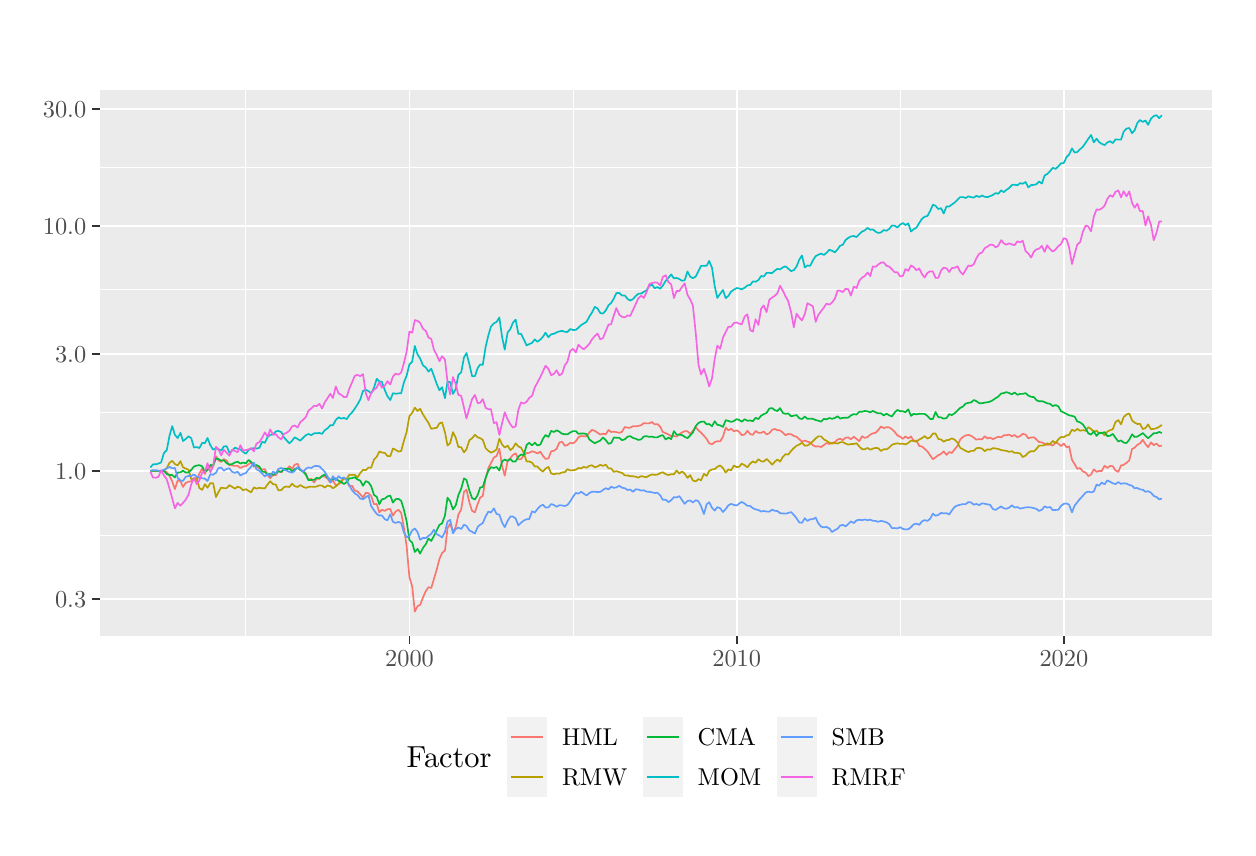
\begin{tikzpicture}[x=1pt,y=1pt]
\definecolor{fillColor}{RGB}{255,255,255}
\path[use as bounding box,fill=fillColor,fill opacity=0.00] (0,0) rectangle (433.62,289.08);
\begin{scope}
\path[clip] (  0.00,  0.00) rectangle (433.62,289.08);
\definecolor{drawColor}{RGB}{255,255,255}
\definecolor{fillColor}{RGB}{255,255,255}

\path[draw=drawColor,line width= 0.6pt,line join=round,line cap=round,fill=fillColor] (  0.00,  0.00) rectangle (433.62,289.08);
\end{scope}
\begin{scope}
\path[clip] ( 26.09, 69.13) rectangle (428.12,266.42);
\definecolor{fillColor}{gray}{0.92}

\path[fill=fillColor] ( 26.09, 69.13) rectangle (428.12,266.42);
\definecolor{drawColor}{RGB}{255,255,255}

\path[draw=drawColor,line width= 0.3pt,line join=round] ( 26.09,105.77) --
	(428.12,105.77);

\path[draw=drawColor,line width= 0.3pt,line join=round] ( 26.09,150.06) --
	(428.12,150.06);

\path[draw=drawColor,line width= 0.3pt,line join=round] ( 26.09,194.35) --
	(428.12,194.35);

\path[draw=drawColor,line width= 0.3pt,line join=round] ( 26.09,238.64) --
	(428.12,238.64);

\path[draw=drawColor,line width= 0.3pt,line join=round] ( 78.85, 69.13) --
	( 78.85,266.42);

\path[draw=drawColor,line width= 0.3pt,line join=round] (197.10, 69.13) --
	(197.10,266.42);

\path[draw=drawColor,line width= 0.3pt,line join=round] (315.33, 69.13) --
	(315.33,266.42);

\path[draw=drawColor,line width= 0.6pt,line join=round] ( 26.09, 82.61) --
	(428.12, 82.61);

\path[draw=drawColor,line width= 0.6pt,line join=round] ( 26.09,128.93) --
	(428.12,128.93);

\path[draw=drawColor,line width= 0.6pt,line join=round] ( 26.09,171.19) --
	(428.12,171.19);

\path[draw=drawColor,line width= 0.6pt,line join=round] ( 26.09,217.51) --
	(428.12,217.51);

\path[draw=drawColor,line width= 0.6pt,line join=round] ( 26.09,259.78) --
	(428.12,259.78);

\path[draw=drawColor,line width= 0.6pt,line join=round] (137.98, 69.13) --
	(137.98,266.42);

\path[draw=drawColor,line width= 0.6pt,line join=round] (256.22, 69.13) --
	(256.22,266.42);

\path[draw=drawColor,line width= 0.6pt,line join=round] (374.43, 69.13) --
	(374.43,266.42);
\definecolor{drawColor}{RGB}{248,118,109}

\path[draw=drawColor,line width= 0.6pt,line join=round] ( 44.36,128.93) --
	( 45.27,128.93) --
	( 46.31,128.93) --
	( 47.28,128.93) --
	( 48.22,128.93) --
	( 49.25,128.93) --
	( 50.26,128.46) --
	( 51.26,127.09) --
	( 52.23,125.08) --
	( 53.20,122.33) --
	( 54.21,125.52) --
	( 55.21,125.16) --
	( 56.15,123.12) --
	( 57.05,124.54) --
	( 58.12,125.01) --
	( 59.09,125.17) --
	( 60.10,126.01) --
	( 61.07,125.20) --
	( 62.04,127.96) --
	( 63.07,129.77) --
	( 64.05,127.77) --
	( 64.98,131.17) --
	( 66.02,130.12) --
	( 67.02,130.66) --
	( 68.03,134.25) --
	( 68.93,132.70) --
	( 69.94,132.19) --
	( 70.88,133.19) --
	( 71.91,132.62) --
	( 72.88,130.99) --
	( 73.82,130.91) --
	( 74.89,130.72) --
	( 75.86,130.72) --
	( 76.86,129.99) --
	( 77.83,130.47) --
	( 78.81,130.66) --
	( 79.84,131.32) --
	( 80.75,131.96) --
	( 81.75,130.45) --
	( 82.66,130.49) --
	( 83.73,129.85) --
	( 84.70,129.36) --
	( 85.70,129.59) --
	( 86.70,127.32) --
	( 87.64,126.29) --
	( 88.68,127.47) --
	( 89.65,127.34) --
	( 90.59,128.98) --
	( 91.66,128.41) --
	( 92.59,129.40) --
	( 93.53,129.44) --
	( 94.57,130.60) --
	( 95.57,129.69) --
	( 96.48,131.16) --
	( 97.55,131.47) --
	( 98.52,129.22) --
	( 99.52,128.93) --
	(100.53,127.99) --
	(101.46,125.66) --
	(102.50,126.09) --
	(103.50,124.71) --
	(104.41,126.06) --
	(105.41,126.05) --
	(106.38,126.96) --
	(107.36,126.89) --
	(108.36,126.11) --
	(109.36,124.68) --
	(110.30,125.42) --
	(111.34,123.69) --
	(112.34,124.18) --
	(113.25,124.66) --
	(114.31,126.48) --
	(115.29,125.60) --
	(116.19,123.45) --
	(117.23,123.55) --
	(118.20,121.74) --
	(119.14,121.57) --
	(120.17,120.47) --
	(121.18,119.32) --
	(122.18,121.00) --
	(123.15,120.85) --
	(124.12,119.81) --
	(125.13,116.88) --
	(126.13,116.96) --
	(127.07,113.92) --
	(127.97,114.87) --
	(129.04,114.45) --
	(130.01,115.11) --
	(131.02,115.13) --
	(131.99,112.73) --
	(132.96,114.27) --
	(134.00,114.89) --
	(134.97,113.71) --
	(135.90,108.72) --
	(136.94,101.67) --
	(137.94, 90.52) --
	(138.95, 87.15) --
	(139.89, 78.10) --
	(140.89, 80.09) --
	(141.80, 80.47) --
	(142.86, 83.21) --
	(143.84, 85.44) --
	(144.84, 86.89) --
	(145.84, 86.62) --
	(146.78, 89.77) --
	(147.82, 93.33) --
	(148.79, 97.08) --
	(149.73, 99.22) --
	(150.79,100.18) --
	(151.70,108.21) --
	(152.67,109.85) --
	(153.68,106.87) --
	(154.68,108.59) --
	(155.62,113.10) --
	(156.65,114.98) --
	(157.66,121.33) --
	(158.56,122.15) --
	(159.63,117.49) --
	(160.60,114.44) --
	(161.61,113.95) --
	(162.61,116.96) --
	(163.52,119.29) --
	(164.45,119.87) --
	(165.49,126.29) --
	(166.49,130.02) --
	(167.40,131.71) --
	(168.47,133.74) --
	(169.44,134.31) --
	(170.44,136.93) --
	(171.45,130.56) --
	(172.39,127.19) --
	(173.42,132.46) --
	(174.42,133.55) --
	(175.33,134.69) --
	(176.33,135.27) --
	(177.31,133.14) --
	(178.28,133.18) --
	(179.28,134.60) --
	(180.28,135.34) --
	(181.22,135.46) --
	(182.26,136.01) --
	(183.26,135.68) --
	(184.17,135.21) --
	(185.24,135.87) --
	(186.21,134.34) --
	(187.11,133.25) --
	(188.18,133.42) --
	(189.15,135.98) --
	(190.16,136.20) --
	(191.13,136.89) --
	(192.10,139.18) --
	(193.13,139.41) --
	(194.10,138.01) --
	(195.04,138.26) --
	(196.08,139.08) --
	(197.08,138.85) --
	(198.09,139.68) --
	(198.99,141.04) --
	(200.00,141.55) --
	(200.93,141.42) --
	(201.97,141.44) --
	(202.94,142.77) --
	(203.88,143.72) --
	(204.95,143.40) --
	(205.92,142.70) --
	(206.92,142.04) --
	(207.89,142.36) --
	(208.87,142.15) --
	(209.90,143.69) --
	(210.81,142.98) --
	(211.81,143.09) --
	(212.72,142.94) --
	(213.79,142.68) --
	(214.76,143.05) --
	(215.76,144.78) --
	(216.76,144.54) --
	(217.70,144.53) --
	(218.74,145.08) --
	(219.71,145.01) --
	(220.65,145.17) --
	(221.72,145.46) --
	(222.62,146.18) --
	(223.59,146.09) --
	(224.60,146.11) --
	(225.60,146.59) --
	(226.54,145.76) --
	(227.57,145.84) --
	(228.58,144.84) --
	(229.48,143.01) --
	(230.55,142.54) --
	(231.52,142.10) --
	(232.53,141.49) --
	(233.53,141.56) --
	(234.47,141.31) --
	(235.47,142.18) --
	(236.44,142.82) --
	(237.41,143.28) --
	(238.42,143.27) --
	(239.42,142.22) --
	(240.36,143.41) --
	(241.40,144.71) --
	(242.40,143.55) --
	(243.31,142.76) --
	(244.37,141.61) --
	(245.35,140.46) --
	(246.25,138.93) --
	(247.29,138.53) --
	(248.26,139.32) --
	(249.20,139.65) --
	(250.23,139.56) --
	(251.24,141.29) --
	(252.24,144.58) --
	(253.21,143.58) --
	(254.18,144.14) --
	(255.19,143.23) --
	(256.19,143.60) --
	(257.13,142.98) --
	(258.03,141.83) --
	(259.10,142.09) --
	(260.07,143.41) --
	(261.08,142.23) --
	(262.05,141.97) --
	(263.02,143.34) --
	(264.05,142.68) --
	(265.03,142.65) --
	(265.96,143.14) --
	(267.00,142.13) --
	(268.00,142.54) --
	(269.01,143.76) --
	(269.91,144.07) --
	(270.92,143.63) --
	(271.86,143.55) --
	(272.89,142.74) --
	(273.86,141.83) --
	(274.80,142.25) --
	(275.87,142.17) --
	(276.84,141.55) --
	(277.84,141.25) --
	(278.82,140.37) --
	(279.79,139.49) --
	(280.82,139.87) --
	(281.76,139.52) --
	(282.73,139.20) --
	(283.74,138.20) --
	(284.74,137.69) --
	(285.68,137.83) --
	(286.71,137.54) --
	(287.72,138.25) --
	(288.62,138.96) --
	(289.69,138.65) --
	(290.66,139.03) --
	(291.67,139.34) --
	(292.67,140.26) --
	(293.58,140.54) --
	(294.51,140.05) --
	(295.55,140.89) --
	(296.55,141.01) --
	(297.46,140.36) --
	(298.53,141.26) --
	(299.50,140.46) --
	(300.50,139.67) --
	(301.51,141.44) --
	(302.44,140.83) --
	(303.48,141.14) --
	(304.48,142.06) --
	(305.39,142.49) --
	(306.39,142.69) --
	(307.36,143.67) --
	(308.34,144.95) --
	(309.34,144.40) --
	(310.34,144.70) --
	(311.28,144.65) --
	(312.32,143.99) --
	(313.32,142.98) --
	(314.23,141.78) --
	(315.30,141.25) --
	(316.27,140.50) --
	(317.17,141.36) --
	(318.21,140.68) --
	(319.18,141.36) --
	(320.12,139.85) --
	(321.15,139.88) --
	(322.16,137.93) --
	(323.16,137.73) --
	(324.13,136.89) --
	(325.10,136.00) --
	(326.11,134.53) --
	(327.11,133.16) --
	(328.05,133.81) --
	(329.05,134.60) --
	(330.06,135.08) --
	(330.99,135.94) --
	(332.03,134.71) --
	(333.00,135.75) --
	(333.94,135.39) --
	(335.01,136.77) --
	(335.98,138.02) --
	(336.98,140.28) --
	(337.95,141.16) --
	(338.92,141.74) --
	(339.96,141.90) --
	(340.87,141.64) --
	(341.87,140.97) --
	(342.78,140.22) --
	(343.85,140.42) --
	(344.82,140.30) --
	(345.82,141.43) --
	(346.82,140.63) --
	(347.76,140.93) --
	(348.80,140.41) --
	(349.77,140.86) --
	(350.71,141.25) --
	(351.78,141.02) --
	(352.68,141.78) --
	(353.65,141.80) --
	(354.66,142.05) --
	(355.66,141.41) --
	(356.60,141.89) --
	(357.63,141.11) --
	(358.64,141.51) --
	(359.54,142.31) --
	(360.61,142.03) --
	(361.58,140.70) --
	(362.59,140.99) --
	(363.59,141.06) --
	(364.50,140.27) --
	(365.44,139.37) --
	(366.47,139.24) --
	(367.47,138.75) --
	(368.38,138.33) --
	(369.45,138.45) --
	(370.42,138.06) --
	(371.42,139.21) --
	(372.43,138.76) --
	(373.37,137.90) --
	(374.40,138.80) --
	(375.41,137.44) --
	(376.31,137.79) --
	(377.35,132.93) --
	(378.32,131.35) --
	(379.26,129.67) --
	(380.29,129.95) --
	(381.30,128.69) --
	(382.30,128.32) --
	(383.27,127.04) --
	(384.24,127.58) --
	(385.25,129.49) --
	(386.25,128.58) --
	(387.19,128.93) --
	(388.09,128.87) --
	(389.16,130.81) --
	(390.13,129.99) --
	(391.14,130.70) --
	(392.11,130.60) --
	(393.08,129.08) --
	(394.11,128.61) --
	(395.09,130.90) --
	(396.02,131.10) --
	(397.06,131.83) --
	(398.06,132.70) --
	(399.07,136.88) --
	(399.97,137.26) --
	(400.98,138.34) --
	(401.92,138.85) --
	(402.95,140.16) --
	(403.92,138.63) --
	(404.86,137.49) --
	(405.93,139.21) --
	(406.90,138.21) --
	(407.90,138.79) --
	(408.87,137.87) --
	(409.85,138.06);
\definecolor{drawColor}{RGB}{183,159,0}

\path[draw=drawColor,line width= 0.6pt,line join=round] ( 44.36,128.93) --
	( 45.27,128.93) --
	( 46.31,128.93) --
	( 47.28,128.93) --
	( 48.22,128.93) --
	( 49.25,128.93) --
	( 50.26,130.00) --
	( 51.26,131.84) --
	( 52.23,132.55) --
	( 53.20,131.40) --
	( 54.21,130.90) --
	( 55.21,132.46) --
	( 56.15,130.16) --
	( 57.05,129.81) --
	( 58.12,129.34) --
	( 59.09,125.96) --
	( 60.10,126.06) --
	( 61.07,126.43) --
	( 62.04,122.70) --
	( 63.07,122.06) --
	( 64.05,124.12) --
	( 64.98,122.84) --
	( 66.02,124.49) --
	( 67.02,124.46) --
	( 68.03,119.44) --
	( 68.93,121.23) --
	( 69.94,122.89) --
	( 70.88,122.71) --
	( 71.91,122.68) --
	( 72.88,123.76) --
	( 73.82,123.18) --
	( 74.89,122.52) --
	( 75.86,123.20) --
	( 76.86,122.86) --
	( 77.83,121.95) --
	( 78.81,122.32) --
	( 79.84,121.69) --
	( 80.75,121.18) --
	( 81.75,122.97) --
	( 82.66,122.51) --
	( 83.73,122.82) --
	( 84.70,122.64) --
	( 85.70,122.63) --
	( 86.70,124.04) --
	( 87.64,125.18) --
	( 88.68,124.10) --
	( 89.65,124.00) --
	( 90.59,121.90) --
	( 91.66,121.98) --
	( 92.59,123.01) --
	( 93.53,123.27) --
	( 94.57,123.11) --
	( 95.57,124.27) --
	( 96.48,123.40) --
	( 97.55,123.10) --
	( 98.52,123.82) --
	( 99.52,123.16) --
	(100.53,122.77) --
	(101.46,123.12) --
	(102.50,123.24) --
	(103.50,123.13) --
	(104.41,123.28) --
	(105.41,123.69) --
	(106.38,123.59) --
	(107.36,122.89) --
	(108.36,123.64) --
	(109.36,123.42) --
	(110.30,122.67) --
	(111.34,123.28) --
	(112.34,124.22) --
	(113.25,125.29) --
	(114.31,126.16) --
	(115.29,126.10) --
	(116.19,127.51) --
	(117.23,127.46) --
	(118.20,127.52) --
	(119.14,126.48) --
	(120.17,128.14) --
	(121.18,129.32) --
	(122.18,129.17) --
	(123.15,130.13) --
	(124.12,130.07) --
	(125.13,133.01) --
	(126.13,134.05) --
	(127.07,135.93) --
	(127.97,135.56) --
	(129.04,135.41) --
	(130.01,134.29) --
	(131.02,134.23) --
	(131.99,137.01) --
	(132.96,136.52) --
	(134.00,135.92) --
	(134.97,136.13) --
	(135.90,139.65) --
	(136.94,142.99) --
	(137.94,148.72) --
	(138.95,149.91) --
	(139.89,151.78) --
	(140.89,150.58) --
	(141.80,151.36) --
	(142.86,149.32) --
	(143.84,147.73) --
	(144.84,146.23) --
	(145.84,144.10) --
	(146.78,144.34) --
	(147.82,144.49) --
	(148.79,146.11) --
	(149.73,146.42) --
	(150.79,142.86) --
	(151.70,138.09) --
	(152.67,138.94) --
	(153.68,142.95) --
	(154.68,140.87) --
	(155.62,137.58) --
	(156.65,137.48) --
	(157.66,135.60) --
	(158.56,136.75) --
	(159.63,140.07) --
	(160.60,140.69) --
	(161.61,141.97) --
	(162.61,141.05) --
	(163.52,140.75) --
	(164.45,140.17) --
	(165.49,137.12) --
	(166.49,136.15) --
	(167.40,135.52) --
	(168.47,135.98) --
	(169.44,136.67) --
	(170.44,140.55) --
	(171.45,138.46) --
	(172.39,137.35) --
	(173.42,138.05) --
	(174.42,136.41) --
	(175.33,137.20) --
	(176.33,138.89) --
	(177.31,137.74) --
	(178.28,137.32) --
	(179.28,135.44) --
	(180.28,132.34) --
	(181.22,132.34) --
	(182.26,131.88) --
	(183.26,130.48) --
	(184.17,130.51) --
	(185.24,129.35) --
	(186.21,128.64) --
	(187.11,129.76) --
	(188.18,130.37) --
	(189.15,128.03) --
	(190.16,127.69) --
	(191.13,127.97) --
	(192.10,127.91) --
	(193.13,128.39) --
	(194.10,128.45) --
	(195.04,129.53) --
	(196.08,129.08) --
	(197.08,129.16) --
	(198.09,129.33) --
	(198.99,129.95) --
	(200.00,129.85) --
	(200.93,130.37) --
	(201.97,130.07) --
	(202.94,130.74) --
	(203.88,130.96) --
	(204.95,130.22) --
	(205.92,130.55) --
	(206.92,131.12) --
	(207.89,130.71) --
	(208.87,131.20) --
	(209.90,129.82) --
	(210.81,129.85) --
	(211.81,128.55) --
	(212.72,128.86) --
	(213.79,128.49) --
	(214.76,128.20) --
	(215.76,127.31) --
	(216.76,127.26) --
	(217.70,127.03) --
	(218.74,126.97) --
	(219.71,126.81) --
	(220.65,126.48) --
	(221.72,127.02) --
	(222.62,126.81) --
	(223.59,126.64) --
	(224.60,127.23) --
	(225.60,127.64) --
	(226.54,127.49) --
	(227.57,127.60) --
	(228.58,128.14) --
	(229.48,128.43) --
	(230.55,127.75) --
	(231.52,127.43) --
	(232.53,127.72) --
	(233.53,127.71) --
	(234.47,129.07) --
	(235.47,127.94) --
	(236.44,128.73) --
	(237.41,127.91) --
	(238.42,126.41) --
	(239.42,127.38) --
	(240.36,125.47) --
	(241.40,125.11) --
	(242.40,125.96) --
	(243.31,125.52) --
	(244.37,127.84) --
	(245.35,127.12) --
	(246.25,128.90) --
	(247.29,129.46) --
	(248.26,129.58) --
	(249.20,130.40) --
	(250.23,130.90) --
	(251.24,129.94) --
	(252.24,128.29) --
	(253.21,129.49) --
	(254.18,129.09) --
	(255.19,130.85) --
	(256.19,130.27) --
	(257.13,130.43) --
	(258.03,131.55) --
	(259.10,130.95) --
	(260.07,130.22) --
	(261.08,131.56) --
	(262.05,132.35) --
	(263.02,131.86) --
	(264.05,133.16) --
	(265.03,132.38) --
	(265.96,132.28) --
	(267.00,133.23) --
	(268.00,132.30) --
	(269.01,131.17) --
	(269.91,132.17) --
	(270.92,133.05) --
	(271.86,132.26) --
	(272.89,133.98) --
	(273.86,134.98) --
	(274.80,134.79) --
	(275.87,136.14) --
	(276.84,137.18) --
	(277.84,138.01) --
	(278.82,138.44) --
	(279.79,139.13) --
	(280.82,138.02) --
	(281.76,138.10) --
	(282.73,138.70) --
	(283.74,139.64) --
	(284.74,140.66) --
	(285.68,141.41) --
	(286.71,141.39) --
	(287.72,140.28) --
	(288.62,139.81) --
	(289.69,139.14) --
	(290.66,138.79) --
	(291.67,138.99) --
	(292.67,138.79) --
	(293.58,139.27) --
	(294.51,139.33) --
	(295.55,138.80) --
	(296.55,138.39) --
	(297.46,138.61) --
	(298.53,138.65) --
	(299.50,138.92) --
	(300.50,137.72) --
	(301.51,136.77) --
	(302.44,136.74) --
	(303.48,137.20) --
	(304.48,136.57) --
	(305.39,136.97) --
	(306.39,137.22) --
	(307.36,137.13) --
	(308.34,136.13) --
	(309.34,136.76) --
	(310.34,136.70) --
	(311.28,137.31) --
	(312.32,138.39) --
	(313.32,138.69) --
	(314.23,138.89) --
	(315.30,138.67) --
	(316.27,138.73) --
	(317.17,138.49) --
	(318.21,139.04) --
	(319.18,139.86) --
	(320.12,139.69) --
	(321.15,139.51) --
	(322.16,140.24) --
	(323.16,140.78) --
	(324.13,141.49) --
	(325.10,140.61) --
	(326.11,141.04) --
	(327.11,142.42) --
	(328.05,142.43) --
	(329.05,140.47) --
	(330.06,140.27) --
	(330.99,139.47) --
	(332.03,140.04) --
	(333.00,140.14) --
	(333.94,140.71) --
	(335.01,140.16) --
	(335.98,139.17) --
	(336.98,137.25) --
	(337.95,136.72) --
	(338.92,136.17) --
	(339.96,135.70) --
	(340.87,136.16) --
	(341.87,136.14) --
	(342.78,137.10) --
	(343.85,137.26) --
	(344.82,136.99) --
	(345.82,136.04) --
	(346.82,136.73) --
	(347.76,136.56) --
	(348.80,137.17) --
	(349.77,137.01) --
	(350.71,136.86) --
	(351.78,136.44) --
	(352.68,136.29) --
	(353.65,136.17) --
	(354.66,135.79) --
	(355.66,136.04) --
	(356.60,135.42) --
	(357.63,135.42) --
	(358.64,135.21) --
	(359.54,133.93) --
	(360.61,134.46) --
	(361.58,135.52) --
	(362.59,136.05) --
	(363.59,135.97) --
	(364.50,136.85) --
	(365.44,138.06) --
	(366.47,138.06) --
	(367.47,138.23) --
	(368.38,138.87) --
	(369.45,138.61) --
	(370.42,139.77) --
	(371.42,138.97) --
	(372.43,140.34) --
	(373.37,141.17) --
	(374.40,141.09) --
	(375.41,141.77) --
	(376.31,141.94) --
	(377.35,143.81) --
	(378.32,143.32) --
	(379.26,144.09) --
	(380.29,143.42) --
	(381.30,143.66) --
	(382.30,143.38) --
	(383.27,144.75) --
	(384.24,144.06) --
	(385.25,143.12) --
	(386.25,143.45) --
	(387.19,142.48) --
	(388.09,142.78) --
	(389.16,141.80) --
	(390.13,143.15) --
	(391.14,143.63) --
	(392.11,144.00) --
	(393.08,146.57) --
	(394.11,147.28) --
	(395.09,145.73) --
	(396.02,148.35) --
	(397.06,149.29) --
	(398.06,149.68) --
	(399.07,147.16) --
	(399.97,146.39) --
	(400.98,145.86) --
	(401.92,145.93) --
	(402.95,144.03) --
	(403.92,144.40) --
	(404.86,145.70) --
	(405.93,143.95) --
	(406.90,144.12) --
	(407.90,144.32) --
	(408.87,144.86) --
	(409.85,145.54);
\definecolor{drawColor}{RGB}{0,186,56}

\path[draw=drawColor,line width= 0.6pt,line join=round] ( 44.36,128.93) --
	( 45.27,128.93) --
	( 46.31,128.93) --
	( 47.28,128.93) --
	( 48.22,128.93) --
	( 49.25,128.93) --
	( 50.26,127.73) --
	( 51.26,127.46) --
	( 52.23,127.41) --
	( 53.20,126.57) --
	( 54.21,128.32) --
	( 55.21,128.41) --
	( 56.15,128.99) --
	( 57.05,128.35) --
	( 58.12,128.37) --
	( 59.09,129.25) --
	( 60.10,130.51) --
	( 61.07,130.84) --
	( 62.04,131.01) --
	( 63.07,130.55) --
	( 64.05,128.58) --
	( 64.98,129.15) --
	( 66.02,131.07) --
	( 67.02,130.86) --
	( 68.03,133.41) --
	( 68.93,133.20) --
	( 69.94,132.63) --
	( 70.88,132.76) --
	( 71.91,131.69) --
	( 72.88,131.21) --
	( 73.82,131.37) --
	( 74.89,131.95) --
	( 75.86,132.23) --
	( 76.86,131.58) --
	( 77.83,131.93) --
	( 78.81,131.63) --
	( 79.84,132.87) --
	( 80.75,132.12) --
	( 81.75,130.79) --
	( 82.66,131.04) --
	( 83.73,130.50) --
	( 84.70,128.73) --
	( 85.70,128.52) --
	( 86.70,127.73) --
	( 87.64,127.79) --
	( 88.68,127.48) --
	( 89.65,128.09) --
	( 90.59,128.71) --
	( 91.66,128.55) --
	( 92.59,129.78) --
	( 93.53,129.56) --
	( 94.57,129.73) --
	( 95.57,128.79) --
	( 96.48,129.57) --
	( 97.55,130.08) --
	( 98.52,129.20) --
	( 99.52,128.69) --
	(100.53,127.49) --
	(101.46,125.58) --
	(102.50,125.65) --
	(103.50,125.68) --
	(104.41,126.38) --
	(105.41,126.21) --
	(106.38,127.08) --
	(107.36,127.65) --
	(108.36,126.55) --
	(109.36,125.70) --
	(110.30,125.79) --
	(111.34,126.26) --
	(112.34,125.33) --
	(113.25,124.91) --
	(114.31,124.17) --
	(115.29,124.91) --
	(116.19,126.19) --
	(117.23,126.30) --
	(118.20,126.63) --
	(119.14,125.82) --
	(120.17,125.43) --
	(121.18,123.54) --
	(122.18,125.23) --
	(123.15,124.80) --
	(124.12,123.42) --
	(125.13,120.25) --
	(126.13,119.54) --
	(127.07,116.89) --
	(127.97,118.60) --
	(129.04,118.91) --
	(130.01,119.69) --
	(131.02,120.01) --
	(131.99,117.44) --
	(132.96,118.70) --
	(134.00,118.83) --
	(134.97,118.09) --
	(135.90,115.05) --
	(136.94,110.67) --
	(137.94,103.94) --
	(138.95,103.01) --
	(139.89, 99.61) --
	(140.89,100.75) --
	(141.80, 99.02) --
	(142.86,101.12) --
	(143.84,102.42) --
	(144.84,104.47) --
	(145.84,103.60) --
	(146.78,105.42) --
	(147.82,107.43) --
	(148.79,109.42) --
	(149.73,109.95) --
	(150.79,112.80) --
	(151.70,119.26) --
	(152.67,117.93) --
	(153.68,114.99) --
	(154.68,116.46) --
	(155.62,120.15) --
	(156.65,122.46) --
	(157.66,126.20) --
	(158.56,125.64) --
	(159.63,121.69) --
	(160.60,119.04) --
	(161.61,118.57) --
	(162.61,120.20) --
	(163.52,122.93) --
	(164.45,123.12) --
	(165.49,126.40) --
	(166.49,129.03) --
	(167.40,130.26) --
	(168.47,129.98) --
	(169.44,130.35) --
	(170.44,129.05) --
	(171.45,132.34) --
	(172.39,133.02) --
	(173.42,132.55) --
	(174.42,133.23) --
	(175.33,132.27) --
	(176.33,132.34) --
	(177.31,134.07) --
	(178.28,134.84) --
	(179.28,134.62) --
	(180.28,138.26) --
	(181.22,139.07) --
	(182.26,138.14) --
	(183.26,139.13) --
	(184.17,138.13) --
	(185.24,138.42) --
	(186.21,140.55) --
	(187.11,141.87) --
	(188.18,141.20) --
	(189.15,143.38) --
	(190.16,142.97) --
	(191.13,143.58) --
	(192.10,143.10) --
	(193.13,142.31) --
	(194.10,142.19) --
	(195.04,142.10) --
	(196.08,142.82) --
	(197.08,143.29) --
	(198.09,143.29) --
	(198.99,142.30) --
	(200.00,142.46) --
	(200.93,142.46) --
	(201.97,142.20) --
	(202.94,140.31) --
	(203.88,139.58) --
	(204.95,138.90) --
	(205.92,139.41) --
	(206.92,139.88) --
	(207.89,141.01) --
	(208.87,140.06) --
	(209.90,138.71) --
	(210.81,138.99) --
	(211.81,141.00) --
	(212.72,140.89) --
	(213.79,140.85) --
	(214.76,140.02) --
	(215.76,140.32) --
	(216.76,141.28) --
	(217.70,141.49) --
	(218.74,140.84) --
	(219.71,140.55) --
	(220.65,140.10) --
	(221.72,140.34) --
	(222.62,141.33) --
	(223.59,141.48) --
	(224.60,141.20) --
	(225.60,141.33) --
	(226.54,141.02) --
	(227.57,141.05) --
	(228.58,141.60) --
	(229.48,141.84) --
	(230.55,140.28) --
	(231.52,140.96) --
	(232.53,140.40) --
	(233.53,143.31) --
	(234.47,142.03) --
	(235.47,141.99) --
	(236.44,141.87) --
	(237.41,141.22) --
	(238.42,140.77) --
	(239.42,141.74) --
	(240.36,142.78) --
	(241.40,145.12) --
	(242.40,146.24) --
	(243.31,146.68) --
	(244.37,146.74) --
	(245.35,145.77) --
	(246.25,145.86) --
	(247.29,145.06) --
	(248.26,146.86) --
	(249.20,145.58) --
	(250.23,145.38) --
	(251.24,144.80) --
	(252.24,147.25) --
	(253.21,146.98) --
	(254.18,146.63) --
	(255.19,146.92) --
	(256.19,147.63) --
	(257.13,147.31) --
	(258.03,146.68) --
	(259.10,147.60) --
	(260.07,147.03) --
	(261.08,147.16) --
	(262.05,146.86) --
	(263.02,148.09) --
	(264.05,147.65) --
	(265.03,148.86) --
	(265.96,149.43) --
	(267.00,149.87) --
	(268.00,151.46) --
	(269.01,151.62) --
	(269.91,150.90) --
	(270.92,150.55) --
	(271.86,151.61) --
	(272.89,149.87) --
	(273.86,149.51) --
	(274.80,149.71) --
	(275.87,148.66) --
	(276.84,148.87) --
	(277.84,149.10) --
	(278.82,147.94) --
	(279.79,147.65) --
	(280.82,148.54) --
	(281.76,147.71) --
	(282.73,147.82) --
	(283.74,147.73) --
	(284.74,147.28) --
	(285.68,147.08) --
	(286.71,146.72) --
	(287.72,147.73) --
	(288.62,147.51) --
	(289.69,148.03) --
	(290.66,147.74) --
	(291.67,148.05) --
	(292.67,148.65) --
	(293.58,147.83) --
	(294.51,148.09) --
	(295.55,148.11) --
	(296.55,148.17) --
	(297.46,148.96) --
	(298.53,149.43) --
	(299.50,149.27) --
	(300.50,150.32) --
	(301.51,150.27) --
	(302.44,150.57) --
	(303.48,150.43) --
	(304.48,150.08) --
	(305.39,150.60) --
	(306.39,150.08) --
	(307.36,149.70) --
	(308.34,149.75) --
	(309.34,148.95) --
	(310.34,149.60) --
	(311.28,149.02) --
	(312.32,148.59) --
	(313.32,150.06) --
	(314.23,150.94) --
	(315.30,150.48) --
	(316.27,150.46) --
	(317.17,150.11) --
	(318.21,151.16) --
	(319.18,148.78) --
	(320.12,149.54) --
	(321.15,149.35) --
	(322.16,149.57) --
	(323.16,149.51) --
	(324.13,149.51) --
	(325.10,148.80) --
	(326.11,147.68) --
	(327.11,147.69) --
	(328.05,150.20) --
	(329.05,148.34) --
	(330.06,148.25) --
	(330.99,147.79) --
	(332.03,148.01) --
	(333.00,149.43) --
	(333.94,149.08) --
	(335.01,149.81) --
	(335.98,150.73) --
	(336.98,151.69) --
	(337.95,152.17) --
	(338.92,153.21) --
	(339.96,153.55) --
	(340.87,153.62) --
	(341.87,154.54) --
	(342.78,154.13) --
	(343.85,153.38) --
	(344.82,153.36) --
	(345.82,153.59) --
	(346.82,153.72) --
	(347.76,153.96) --
	(348.80,154.51) --
	(349.77,155.19) --
	(350.71,155.78) --
	(351.78,156.88) --
	(352.68,157.03) --
	(353.65,157.38) --
	(354.66,157.03) --
	(355.66,156.57) --
	(356.60,157.27) --
	(357.63,156.43) --
	(358.64,156.76) --
	(359.54,156.75) --
	(360.61,157.02) --
	(361.58,156.12) --
	(362.59,155.70) --
	(363.59,155.58) --
	(364.50,154.51) --
	(365.44,154.05) --
	(366.47,154.13) --
	(367.47,153.81) --
	(368.38,153.34) --
	(369.45,153.15) --
	(370.42,152.34) --
	(371.42,152.72) --
	(372.43,152.25) --
	(373.37,150.51) --
	(374.40,149.99) --
	(375.41,149.49) --
	(376.31,149.01) --
	(377.35,148.80) --
	(378.32,148.50) --
	(379.26,146.80) --
	(380.29,146.47) --
	(381.30,145.70) --
	(382.30,144.21) --
	(383.27,142.46) --
	(384.24,142.04) --
	(385.25,143.19) --
	(386.25,141.58) --
	(387.19,142.68) --
	(388.09,142.57) --
	(389.16,142.92) --
	(390.13,141.46) --
	(391.14,141.62) --
	(392.11,142.29) --
	(393.08,140.89) --
	(394.11,139.54) --
	(395.09,139.93) --
	(396.02,139.15) --
	(397.06,138.98) --
	(398.06,140.19) --
	(399.07,142.16) --
	(399.97,141.18) --
	(400.98,141.31) --
	(401.92,141.88) --
	(402.95,142.58) --
	(403.92,141.59) --
	(404.86,140.74) --
	(405.93,141.64) --
	(406.90,142.55) --
	(407.90,142.56) --
	(408.87,142.99) --
	(409.85,142.62);
\definecolor{drawColor}{RGB}{0,191,196}

\path[draw=drawColor,line width= 0.6pt,line join=round] ( 44.36,130.15) --
	( 45.27,131.29) --
	( 46.31,131.30) --
	( 47.28,131.58) --
	( 48.22,131.97) --
	( 49.25,135.40) --
	( 50.26,136.42) --
	( 51.26,141.66) --
	( 52.23,145.09) --
	( 53.20,141.96) --
	( 54.21,140.78) --
	( 55.21,142.67) --
	( 56.15,139.71) --
	( 57.05,140.41) --
	( 58.12,141.40) --
	( 59.09,140.77) --
	( 60.10,137.36) --
	( 61.07,137.53) --
	( 62.04,137.16) --
	( 63.07,139.06) --
	( 64.05,138.96) --
	( 64.98,140.81) --
	( 66.02,138.13) --
	( 67.02,136.59) --
	( 68.03,137.09) --
	( 68.93,136.75) --
	( 69.94,136.24) --
	( 70.88,137.74) --
	( 71.91,137.87) --
	( 72.88,135.50) --
	( 73.82,136.17) --
	( 74.89,137.33) --
	( 75.86,136.93) --
	( 76.86,136.68) --
	( 77.83,135.81) --
	( 78.81,135.09) --
	( 79.84,136.48) --
	( 80.75,136.92) --
	( 81.75,137.17) --
	( 82.66,136.98) --
	( 83.73,137.26) --
	( 84.70,139.44) --
	( 85.70,139.06) --
	( 86.70,141.17) --
	( 87.64,141.94) --
	( 88.68,142.09) --
	( 89.65,143.19) --
	( 90.59,143.37) --
	( 91.66,142.92) --
	( 92.59,141.04) --
	( 93.53,139.99) --
	( 94.57,138.86) --
	( 95.57,139.84) --
	( 96.48,141.06) --
	( 97.55,140.44) --
	( 98.52,139.84) --
	( 99.52,140.90) --
	(100.53,141.81) --
	(101.46,142.26) --
	(102.50,141.83) --
	(103.50,142.49) --
	(104.41,142.52) --
	(105.41,142.62) --
	(106.38,142.32) --
	(107.36,143.63) --
	(108.36,144.31) --
	(109.36,145.40) --
	(110.30,145.38) --
	(111.34,147.32) --
	(112.34,148.29) --
	(113.25,147.82) --
	(114.31,148.06) --
	(115.29,147.63) --
	(116.19,149.00) --
	(117.23,150.09) --
	(118.20,151.42) --
	(119.14,152.88) --
	(120.17,154.72) --
	(121.18,157.82) --
	(122.18,158.24) --
	(123.15,157.75) --
	(124.12,156.93) --
	(125.13,158.95) --
	(126.13,162.20) --
	(127.07,161.24) --
	(127.97,161.11) --
	(129.04,158.12) --
	(130.01,155.90) --
	(131.02,154.51) --
	(131.99,156.98) --
	(132.96,156.80) --
	(134.00,156.94) --
	(134.97,156.97) --
	(135.90,160.74) --
	(136.94,163.38) --
	(137.94,167.39) --
	(138.95,168.38) --
	(139.89,174.04) --
	(140.89,171.00) --
	(141.80,169.55) --
	(142.86,167.04) --
	(143.84,166.30) --
	(144.84,164.79) --
	(145.84,165.85) --
	(146.78,163.27) --
	(147.82,160.35) --
	(148.79,158.05) --
	(149.73,159.16) --
	(150.79,155.20) --
	(151.70,161.14) --
	(152.67,161.00) --
	(153.68,156.73) --
	(154.68,158.49) --
	(155.62,163.65) --
	(156.65,164.52) --
	(157.66,169.91) --
	(158.56,171.51) --
	(159.63,167.35) --
	(160.60,163.13) --
	(161.61,163.18) --
	(162.61,166.09) --
	(163.52,167.38) --
	(164.45,167.21) --
	(165.49,173.80) --
	(166.49,177.99) --
	(167.40,181.04) --
	(168.47,182.26) --
	(169.44,182.73) --
	(170.44,184.34) --
	(171.45,177.15) --
	(172.39,172.73) --
	(173.42,178.92) --
	(174.42,180.17) --
	(175.33,182.50) --
	(176.33,183.58) --
	(177.31,178.45) --
	(178.28,178.42) --
	(179.28,176.48) --
	(180.28,174.26) --
	(181.22,174.71) --
	(182.26,175.19) --
	(183.26,176.44) --
	(184.17,175.56) --
	(185.24,176.38) --
	(186.21,177.39) --
	(187.11,178.85) --
	(188.18,177.23) --
	(189.15,178.29) --
	(190.16,178.45) --
	(191.13,178.98) --
	(192.10,179.33) --
	(193.13,179.52) --
	(194.10,179.19) --
	(195.04,179.11) --
	(196.08,180.19) --
	(197.08,179.82) --
	(198.09,179.90) --
	(198.99,180.64) --
	(200.00,181.61) --
	(200.93,182.17) --
	(201.97,182.81) --
	(202.94,184.65) --
	(203.88,186.11) --
	(204.95,188.20) --
	(205.92,187.60) --
	(206.92,185.97) --
	(207.89,185.77) --
	(208.87,186.85) --
	(209.90,188.82) --
	(210.81,189.54) --
	(211.81,191.22) --
	(212.72,193.17) --
	(213.79,193.20) --
	(214.76,192.29) --
	(215.76,192.34) --
	(216.76,191.07) --
	(217.70,190.47) --
	(218.74,191.01) --
	(219.71,192.10) --
	(220.65,192.94) --
	(221.72,193.02) --
	(222.62,193.61) --
	(223.59,194.17) --
	(224.60,195.70) --
	(225.60,196.26) --
	(226.54,194.92) --
	(227.57,195.34) --
	(228.58,194.75) --
	(229.48,195.84) --
	(230.55,197.61) --
	(231.52,198.69) --
	(232.53,199.90) --
	(233.53,198.47) --
	(234.47,198.66) --
	(235.47,198.25) --
	(236.44,197.63) --
	(237.41,197.81) --
	(238.42,200.97) --
	(239.42,199.08) --
	(240.36,198.56) --
	(241.40,199.14) --
	(242.40,201.18) --
	(243.31,203.01) --
	(244.37,203.02) --
	(245.35,203.03) --
	(246.25,204.81) --
	(247.29,202.27) --
	(248.26,195.66) --
	(249.20,191.43) --
	(250.23,192.92) --
	(251.24,194.31) --
	(252.24,191.35) --
	(253.21,192.15) --
	(254.18,193.71) --
	(255.19,194.39) --
	(256.19,195.00) --
	(257.13,194.84) --
	(258.03,194.54) --
	(259.10,195.11) --
	(260.07,195.93) --
	(261.08,196.10) --
	(262.05,197.38) --
	(263.02,197.28) --
	(264.05,197.87) --
	(265.03,199.35) --
	(265.96,199.12) --
	(267.00,200.49) --
	(268.00,200.46) --
	(269.01,200.42) --
	(269.91,201.22) --
	(270.92,201.95) --
	(271.86,201.71) --
	(272.89,202.47) --
	(273.86,202.85) --
	(274.80,202.03) --
	(275.87,201.11) --
	(276.84,201.46) --
	(277.84,202.78) --
	(278.82,205.27) --
	(279.79,206.76) --
	(280.82,202.43) --
	(281.76,203.14) --
	(282.73,203.01) --
	(283.74,204.98) --
	(284.74,206.52) --
	(285.68,207.02) --
	(286.71,207.46) --
	(287.72,206.93) --
	(288.62,207.71) --
	(289.69,208.83) --
	(290.66,208.46) --
	(291.67,207.90) --
	(292.67,209.00) --
	(293.58,210.29) --
	(294.51,210.59) --
	(295.55,212.34) --
	(296.55,213.14) --
	(297.46,213.63) --
	(298.53,213.80) --
	(299.50,213.40) --
	(300.50,214.48) --
	(301.51,215.40) --
	(302.44,215.79) --
	(303.48,216.72) --
	(304.48,216.05) --
	(305.39,216.21) --
	(306.39,215.38) --
	(307.36,214.90) --
	(308.34,215.09) --
	(309.34,215.94) --
	(310.34,215.70) --
	(311.28,216.33) --
	(312.32,217.59) --
	(313.32,217.51) --
	(314.23,216.85) --
	(315.30,217.93) --
	(316.27,218.49) --
	(317.17,217.75) --
	(318.21,218.34) --
	(319.18,215.41) --
	(320.12,216.23) --
	(321.15,216.81) --
	(322.16,218.52) --
	(323.16,219.99) --
	(324.13,220.80) --
	(325.10,220.99) --
	(326.11,222.85) --
	(327.11,225.09) --
	(328.05,224.73) --
	(329.05,223.54) --
	(330.06,223.87) --
	(330.99,221.93) --
	(332.03,224.51) --
	(333.00,224.44) --
	(333.94,225.16) --
	(335.01,225.91) --
	(335.98,226.91) --
	(336.98,227.86) --
	(337.95,227.86) --
	(338.92,227.53) --
	(339.96,228.15) --
	(340.87,227.83) --
	(341.87,227.66) --
	(342.78,228.33) --
	(343.85,227.89) --
	(344.82,228.42) --
	(345.82,227.98) --
	(346.82,227.84) --
	(347.76,228.17) --
	(348.80,228.64) --
	(349.77,229.30) --
	(350.71,229.08) --
	(351.78,230.29) --
	(352.68,229.66) --
	(353.65,230.45) --
	(354.66,231.13) --
	(355.66,232.23) --
	(356.60,232.35) --
	(357.63,232.13) --
	(358.64,232.90) --
	(359.54,232.68) --
	(360.61,233.31) --
	(361.58,231.35) --
	(362.59,232.20) --
	(363.59,232.27) --
	(364.50,232.50) --
	(365.44,233.49) --
	(366.47,232.76) --
	(367.47,235.67) --
	(368.38,236.18) --
	(369.45,237.26) --
	(370.42,238.44) --
	(371.42,238.04) --
	(372.43,238.95) --
	(373.37,240.05) --
	(374.40,240.18) --
	(375.41,242.32) --
	(376.31,243.22) --
	(377.35,245.46) --
	(378.32,243.95) --
	(379.26,244.15) --
	(380.29,245.16) --
	(381.30,246.05) --
	(382.30,247.49) --
	(383.27,248.95) --
	(384.24,250.29) --
	(385.25,247.65) --
	(386.25,248.98) --
	(387.19,247.68) --
	(388.09,247.11) --
	(389.16,246.65) --
	(390.13,247.59) --
	(391.14,248.05) --
	(392.11,247.36) --
	(393.08,248.73) --
	(394.11,248.62) --
	(395.09,248.61) --
	(396.02,251.50) --
	(397.06,252.60) --
	(398.06,252.82) --
	(399.07,250.95) --
	(399.97,251.96) --
	(400.98,254.66) --
	(401.92,255.69) --
	(402.95,255.04) --
	(403.92,255.55) --
	(404.86,253.97) --
	(405.93,256.24) --
	(406.90,257.12) --
	(407.90,257.45) --
	(408.87,256.38) --
	(409.85,257.41);
\definecolor{drawColor}{RGB}{97,156,255}

\path[draw=drawColor,line width= 0.6pt,line join=round] ( 44.36,128.94) --
	( 45.27,129.20) --
	( 46.31,129.17) --
	( 47.28,129.00) --
	( 48.22,128.92) --
	( 49.25,129.37) --
	( 50.26,129.82) --
	( 51.26,130.35) --
	( 52.23,129.90) --
	( 53.20,129.96) --
	( 54.21,126.38) --
	( 55.21,125.48) --
	( 56.15,125.29) --
	( 57.05,126.76) --
	( 58.12,127.11) --
	( 59.09,127.06) --
	( 60.10,127.63) --
	( 61.07,126.83) --
	( 62.04,126.59) --
	( 63.07,126.24) --
	( 64.05,126.14) --
	( 64.98,125.25) --
	( 66.02,127.75) --
	( 67.02,127.53) --
	( 68.03,128.24) --
	( 68.93,129.95) --
	( 69.94,130.11) --
	( 70.88,128.98) --
	( 71.91,129.64) --
	( 72.88,129.85) --
	( 73.82,128.65) --
	( 74.89,128.18) --
	( 75.86,128.67) --
	( 76.86,127.26) --
	( 77.83,127.80) --
	( 78.81,128.11) --
	( 79.84,129.44) --
	( 80.75,130.46) --
	( 81.75,131.91) --
	( 82.66,129.49) --
	( 83.73,128.94) --
	( 84.70,128.01) --
	( 85.70,126.89) --
	( 86.70,127.87) --
	( 87.64,126.88) --
	( 88.68,128.71) --
	( 89.65,128.01) --
	( 90.59,129.62) --
	( 91.66,130.03) --
	( 92.59,129.32) --
	( 93.53,129.06) --
	( 94.57,128.56) --
	( 95.57,128.32) --
	( 96.48,128.90) --
	( 97.55,130.31) --
	( 98.52,129.60) --
	( 99.52,128.58) --
	(100.53,129.70) --
	(101.46,130.21) --
	(102.50,129.96) --
	(103.50,130.63) --
	(104.41,130.71) --
	(105.41,130.59) --
	(106.38,129.57) --
	(107.36,128.59) --
	(108.36,126.82) --
	(109.36,124.88) --
	(110.30,126.99) --
	(111.34,125.43) --
	(112.34,127.03) --
	(113.25,126.22) --
	(114.31,126.49) --
	(115.29,125.63) --
	(116.19,123.71) --
	(117.23,121.95) --
	(118.20,120.77) --
	(119.14,120.24) --
	(120.17,118.94) --
	(121.18,118.68) --
	(122.18,119.43) --
	(123.15,120.01) --
	(124.12,116.21) --
	(125.13,114.70) --
	(126.13,113.36) --
	(127.07,112.76) --
	(127.97,112.87) --
	(129.04,111.46) --
	(130.01,111.06) --
	(131.02,113.25) --
	(131.99,110.50) --
	(132.96,110.13) --
	(134.00,110.48) --
	(134.97,110.04) --
	(135.90,106.80) --
	(136.94,104.96) --
	(137.94,105.37) --
	(138.95,107.45) --
	(139.89,108.10) --
	(140.89,106.76) --
	(141.80,104.03) --
	(142.86,104.73) --
	(143.84,104.61) --
	(144.84,105.45) --
	(145.84,106.16) --
	(146.78,107.67) --
	(147.82,106.00) --
	(148.79,105.54) --
	(149.73,104.86) --
	(150.79,106.85) --
	(151.70,110.61) --
	(152.67,111.24) --
	(153.68,106.39) --
	(154.68,107.92) --
	(155.62,108.44) --
	(156.65,107.93) --
	(157.66,109.46) --
	(158.56,109.05) --
	(159.63,107.37) --
	(160.60,106.91) --
	(161.61,106.30) --
	(162.61,108.70) --
	(163.52,109.48) --
	(164.45,110.05) --
	(165.49,112.53) --
	(166.49,114.23) --
	(167.40,113.86) --
	(168.47,115.38) --
	(169.44,113.34) --
	(170.44,113.12) --
	(171.45,110.22) --
	(172.39,108.58) --
	(173.42,110.86) --
	(174.42,112.42) --
	(175.33,112.47) --
	(176.33,111.68) --
	(177.31,109.24) --
	(178.28,110.19) --
	(179.28,110.99) --
	(180.28,111.46) --
	(181.22,111.47) --
	(182.26,114.31) --
	(183.26,113.88) --
	(184.17,115.11) --
	(185.24,116.26) --
	(186.21,116.70) --
	(187.11,115.67) --
	(188.18,115.75) --
	(189.15,116.93) --
	(190.16,116.61) --
	(191.13,115.95) --
	(192.10,116.50) --
	(193.13,116.45) --
	(194.10,116.23) --
	(195.04,116.61) --
	(196.08,117.93) --
	(197.08,119.63) --
	(198.09,120.98) --
	(198.99,120.67) --
	(200.00,121.41) --
	(200.93,120.72) --
	(201.97,120.03) --
	(202.94,120.89) --
	(203.88,121.40) --
	(204.95,121.39) --
	(205.92,121.29) --
	(206.92,121.34) --
	(207.89,122.03) --
	(208.87,122.66) --
	(209.90,122.24) --
	(210.81,123.21) --
	(211.81,122.79) --
	(212.72,122.96) --
	(213.79,123.53) --
	(214.76,122.85) --
	(215.76,122.67) --
	(216.76,122.02) --
	(217.70,122.19) --
	(218.74,121.38) --
	(219.71,122.28) --
	(220.65,122.19) --
	(221.72,121.80) --
	(222.62,121.93) --
	(223.59,121.44) --
	(224.60,121.33) --
	(225.60,121.18) --
	(226.54,120.94) --
	(227.57,121.01) --
	(228.58,120.06) --
	(229.48,118.50) --
	(230.55,118.52) --
	(231.52,117.64) --
	(232.53,118.32) --
	(233.53,119.45) --
	(234.47,119.32) --
	(235.47,119.81) --
	(236.44,118.38) --
	(237.41,117.02) --
	(238.42,118.06) --
	(239.42,118.22) --
	(240.36,117.52) --
	(241.40,118.32) --
	(242.40,117.96) --
	(243.31,116.20) --
	(244.37,113.32) --
	(245.35,116.86) --
	(246.25,117.59) --
	(247.29,115.60) --
	(248.26,114.58) --
	(249.20,115.84) --
	(250.23,115.43) --
	(251.24,114.05) --
	(252.24,115.16) --
	(253.21,116.50) --
	(254.18,116.99) --
	(255.19,116.62) --
	(256.19,116.40) --
	(257.13,117.15) --
	(258.03,117.71) --
	(259.10,117.10) --
	(260.07,116.29) --
	(261.08,116.26) --
	(262.05,115.42) --
	(263.02,115.03) --
	(264.05,114.78) --
	(265.03,114.24) --
	(265.96,114.43) --
	(267.00,114.23) --
	(268.00,114.18) --
	(269.01,114.92) --
	(269.91,114.49) --
	(270.92,114.42) --
	(271.86,113.64) --
	(272.89,113.54) --
	(273.86,113.47) --
	(274.80,113.70) --
	(275.87,114.04) --
	(276.84,113.00) --
	(277.84,111.79) --
	(278.82,110.29) --
	(279.79,110.17) --
	(280.82,111.81) --
	(281.76,110.84) --
	(282.73,111.44) --
	(283.74,111.49) --
	(284.74,112.04) --
	(285.68,110.00) --
	(286.71,108.76) --
	(287.72,108.53) --
	(288.62,108.67) --
	(289.69,108.14) --
	(290.66,106.82) --
	(291.67,107.54) --
	(292.67,108.03) --
	(293.58,109.17) --
	(294.51,109.41) --
	(295.55,108.89) --
	(296.55,109.75) --
	(297.46,110.66) --
	(298.53,110.07) --
	(299.50,111.04) --
	(300.50,111.27) --
	(301.51,111.11) --
	(302.44,111.36) --
	(303.48,111.10) --
	(304.48,111.30) --
	(305.39,110.90) --
	(306.39,110.83) --
	(307.36,110.53) --
	(308.34,110.88) --
	(309.34,110.63) --
	(310.34,110.31) --
	(311.28,109.75) --
	(312.32,108.23) --
	(313.32,108.26) --
	(314.23,108.13) --
	(315.30,108.56) --
	(316.27,107.95) --
	(317.17,107.77) --
	(318.21,107.83) --
	(319.18,108.59) --
	(320.12,109.57) --
	(321.15,109.87) --
	(322.16,109.43) --
	(323.16,110.67) --
	(324.13,111.15) --
	(325.10,110.83) --
	(326.11,111.64) --
	(327.11,113.50) --
	(328.05,112.71) --
	(329.05,113.01) --
	(330.06,113.75) --
	(330.99,113.55) --
	(332.03,113.65) --
	(333.00,113.16) --
	(333.94,114.59) --
	(335.01,115.99) --
	(335.98,116.42) --
	(336.98,116.68) --
	(337.95,116.92) --
	(338.92,116.91) --
	(339.96,117.66) --
	(340.87,117.53) --
	(341.87,116.71) --
	(342.78,116.98) --
	(343.85,116.57) --
	(344.82,117.20) --
	(345.82,117.05) --
	(346.82,116.83) --
	(347.76,116.65) --
	(348.80,115.14) --
	(349.77,114.81) --
	(350.71,115.46) --
	(351.78,116.09) --
	(352.68,115.41) --
	(353.65,115.24) --
	(354.66,115.65) --
	(355.66,116.48) --
	(356.60,115.70) --
	(357.63,115.85) --
	(358.64,115.30) --
	(359.54,115.49) --
	(360.61,115.74) --
	(361.58,115.77) --
	(362.59,115.72) --
	(363.59,115.46) --
	(364.50,115.21) --
	(365.44,114.44) --
	(366.47,114.89) --
	(367.47,116.13) --
	(368.38,115.67) --
	(369.45,115.86) --
	(370.42,114.72) --
	(371.42,114.81) --
	(372.43,114.86) --
	(373.37,116.26) --
	(374.40,117.03) --
	(375.41,117.14) --
	(376.31,116.71) --
	(377.35,113.95) --
	(378.32,116.39) --
	(379.26,117.58) --
	(380.29,118.88) --
	(381.30,119.95) --
	(382.30,121.08) --
	(383.27,121.46) --
	(384.24,121.13) --
	(385.25,121.47) --
	(386.25,123.98) --
	(387.19,123.58) --
	(388.09,124.72) --
	(389.16,124.06) --
	(390.13,125.50) --
	(391.14,124.98) --
	(392.11,124.43) --
	(393.08,124.17) --
	(394.11,124.85) --
	(395.09,124.21) --
	(396.02,124.45) --
	(397.06,124.33) --
	(398.06,123.84) --
	(399.07,123.57) --
	(399.97,122.65) --
	(400.98,122.74) --
	(401.92,122.26) --
	(402.95,122.10) --
	(403.92,121.37) --
	(404.86,121.58) --
	(405.93,121.03) --
	(406.90,119.87) --
	(407.90,119.48) --
	(408.87,118.64) --
	(409.85,118.92);
\definecolor{drawColor}{RGB}{245,100,227}

\path[draw=drawColor,line width= 0.6pt,line join=round] ( 44.36,128.62) --
	( 45.27,126.55) --
	( 46.31,126.44) --
	( 47.28,126.81) --
	( 48.22,129.18) --
	( 49.25,127.29) --
	( 50.26,125.91) --
	( 51.26,122.48) --
	( 52.23,119.03) --
	( 53.20,115.37) --
	( 54.21,117.36) --
	( 55.21,116.36) --
	( 56.15,117.38) --
	( 57.05,118.46) --
	( 58.12,120.31) --
	( 59.09,123.99) --
	( 60.10,126.40) --
	( 61.07,124.09) --
	( 62.04,125.45) --
	( 63.07,128.37) --
	( 64.05,128.65) --
	( 64.98,131.70) --
	( 66.02,128.40) --
	( 67.02,130.63) --
	( 68.03,137.62) --
	( 68.93,136.77) --
	( 69.94,134.55) --
	( 70.88,136.54) --
	( 71.91,135.43) --
	( 72.88,134.41) --
	( 73.82,136.57) --
	( 74.89,136.11) --
	( 75.86,135.70) --
	( 76.86,138.22) --
	( 77.83,136.20) --
	( 78.81,136.45) --
	( 79.84,136.70) --
	( 80.75,137.13) --
	( 81.75,135.98) --
	( 82.66,138.73) --
	( 83.73,139.37) --
	( 84.70,140.83) --
	( 85.70,142.86) --
	( 86.70,141.26) --
	( 87.64,143.90) --
	( 88.68,141.96) --
	( 89.65,142.20) --
	( 90.59,141.06) --
	( 91.66,140.28) --
	( 92.59,142.30) --
	( 93.53,142.66) --
	( 94.57,143.45) --
	( 95.57,144.99) --
	( 96.48,145.34) --
	( 97.55,144.61) --
	( 98.52,146.56) --
	( 99.52,147.37) --
	(100.53,148.42) --
	(101.46,150.68) --
	(102.50,151.48) --
	(103.50,152.52) --
	(104.41,152.31) --
	(105.41,153.15) --
	(106.38,151.45) --
	(107.36,153.71) --
	(108.36,155.21) --
	(109.36,156.79) --
	(110.30,155.24) --
	(111.34,159.44) --
	(112.34,156.94) --
	(113.25,156.44) --
	(114.31,155.56) --
	(115.29,155.66) --
	(116.19,158.53) --
	(117.23,160.96) --
	(118.20,163.29) --
	(119.14,163.63) --
	(120.17,163.17) --
	(121.18,163.88) --
	(122.18,156.99) --
	(123.15,154.46) --
	(124.12,157.04) --
	(125.13,158.23) --
	(126.13,159.02) --
	(127.07,161.08) --
	(127.97,159.00) --
	(129.04,159.71) --
	(130.01,161.35) --
	(131.02,160.15) --
	(131.99,163.01) --
	(132.96,164.05) --
	(134.00,163.73) --
	(134.97,164.46) --
	(135.90,167.71) --
	(136.94,172.04) --
	(137.94,179.28) --
	(138.95,178.84) --
	(139.89,183.43) --
	(140.89,183.11) --
	(141.80,182.44) --
	(142.86,180.28) --
	(143.84,179.54) --
	(144.84,177.08) --
	(145.84,176.61) --
	(146.78,172.78) --
	(147.82,170.78) --
	(148.79,168.53) --
	(149.73,170.35) --
	(150.79,169.17) --
	(151.70,161.16) --
	(152.67,156.52) --
	(153.68,162.85) --
	(154.68,160.30) --
	(155.62,156.36) --
	(156.65,156.04) --
	(157.66,151.76) --
	(158.56,147.85) --
	(159.63,151.67) --
	(160.60,154.88) --
	(161.61,156.37) --
	(162.61,153.44) --
	(163.52,153.52) --
	(164.45,154.87) --
	(165.49,151.71) --
	(166.49,151.21) --
	(167.40,151.19) --
	(168.47,146.20) --
	(169.44,146.51) --
	(170.44,141.91) --
	(171.45,146.24) --
	(172.39,150.10) --
	(173.42,147.57) --
	(174.42,145.74) --
	(175.33,144.58) --
	(176.33,145.01) --
	(177.31,151.01) --
	(178.28,153.66) --
	(179.28,153.26) --
	(180.28,153.91) --
	(181.22,155.28) --
	(182.26,156.09) --
	(183.26,159.12) --
	(184.17,160.78) --
	(185.24,162.81) --
	(186.21,164.91) --
	(187.11,166.89) --
	(188.18,165.79) --
	(189.15,163.50) --
	(190.16,164.00) --
	(191.13,165.26) --
	(192.10,163.42) --
	(193.13,164.10) --
	(194.10,167.07) --
	(195.04,168.37) --
	(196.08,172.36) --
	(197.08,173.00) --
	(198.09,171.71) --
	(198.99,174.49) --
	(200.00,173.53) --
	(200.93,172.86) --
	(201.97,173.77) --
	(202.94,174.79) --
	(203.88,176.40) --
	(204.95,177.65) --
	(205.92,178.54) --
	(206.92,176.45) --
	(207.89,176.91) --
	(208.87,179.34) --
	(209.90,181.80) --
	(210.81,181.89) --
	(211.81,185.14) --
	(212.72,187.77) --
	(213.79,185.31) --
	(214.76,184.60) --
	(215.76,184.40) --
	(216.76,185.09) --
	(217.70,184.91) --
	(218.74,187.07) --
	(219.71,189.19) --
	(220.65,191.30) --
	(221.72,192.22) --
	(222.62,191.41) --
	(223.59,193.37) --
	(224.60,196.38) --
	(225.60,196.83) --
	(226.54,197.01) --
	(227.57,196.94) --
	(228.58,195.88) --
	(229.48,198.99) --
	(230.55,199.61) --
	(231.52,197.16) --
	(232.53,196.33) --
	(233.53,191.34) --
	(234.47,193.94) --
	(235.47,193.90) --
	(236.44,195.40) --
	(237.41,196.68) --
	(238.42,192.55) --
	(239.42,190.88) --
	(240.36,188.69) --
	(241.40,178.75) --
	(242.40,167.30) --
	(243.31,163.75) --
	(244.37,165.77) --
	(245.35,162.77) --
	(246.25,159.44) --
	(247.29,162.42) --
	(248.26,169.38) --
	(249.20,174.17) --
	(250.23,173.04) --
	(251.24,177.05) --
	(252.24,179.14) --
	(253.21,181.04) --
	(254.18,181.03) --
	(255.19,182.34) --
	(256.19,182.55) --
	(257.13,182.08) --
	(258.03,181.89) --
	(259.10,184.75) --
	(260.07,185.50) --
	(261.08,179.73) --
	(262.05,179.25) --
	(263.02,183.70) --
	(264.05,181.66) --
	(265.03,187.53) --
	(265.96,188.72) --
	(267.00,186.30) --
	(268.00,190.77) --
	(269.01,191.57) --
	(269.91,192.14) --
	(270.92,193.14) --
	(271.86,195.81) --
	(272.89,194.04) --
	(273.86,191.98) --
	(274.80,190.32) --
	(275.87,186.24) --
	(276.84,180.81) --
	(277.84,185.74) --
	(278.82,184.32) --
	(279.79,183.29) --
	(280.82,185.65) --
	(281.76,189.50) --
	(282.73,188.99) --
	(283.74,188.41) --
	(284.74,182.77) --
	(285.68,185.26) --
	(286.71,186.66) --
	(287.72,187.96) --
	(288.62,189.35) --
	(289.69,188.99) --
	(290.66,189.76) --
	(291.67,191.15) --
	(292.67,194.13) --
	(293.58,193.97) --
	(294.51,193.54) --
	(295.55,194.72) --
	(296.55,194.54) --
	(297.46,192.26) --
	(298.53,195.54) --
	(299.50,194.99) --
	(300.50,197.66) --
	(301.51,198.77) --
	(302.44,199.31) --
	(303.48,200.58) --
	(304.48,199.33) --
	(305.39,202.84) --
	(306.39,202.67) --
	(307.36,203.49) --
	(308.34,204.20) --
	(309.34,204.26) --
	(310.34,203.01) --
	(311.28,202.77) --
	(312.32,201.74) --
	(313.32,200.65) --
	(314.23,200.69) --
	(315.30,199.18) --
	(316.27,199.42) --
	(317.17,201.86) --
	(318.21,201.23) --
	(319.18,203.15) --
	(320.12,202.60) --
	(321.15,201.44) --
	(322.16,202.07) --
	(323.16,200.04) --
	(324.13,198.82) --
	(325.10,200.44) --
	(326.11,201.04) --
	(327.11,200.95) --
	(328.05,198.65) --
	(329.05,198.67) --
	(330.06,201.38) --
	(330.99,202.34) --
	(332.03,202.11) --
	(333.00,200.81) --
	(333.94,202.20) --
	(335.01,202.32) --
	(335.98,202.86) --
	(336.98,200.87) --
	(337.95,199.88) --
	(338.92,201.51) --
	(339.96,203.17) --
	(340.87,202.92) --
	(341.87,203.60) --
	(342.78,205.69) --
	(343.85,207.40) --
	(344.82,207.77) --
	(345.82,209.38) --
	(346.82,209.96) --
	(347.76,210.64) --
	(348.80,210.60) --
	(349.77,209.71) --
	(350.71,210.25) --
	(351.78,212.30) --
	(352.68,211.18) --
	(353.65,210.64) --
	(354.66,211.15) --
	(355.66,210.75) --
	(356.60,210.47) --
	(357.63,211.89) --
	(358.64,211.52) --
	(359.54,212.11) --
	(360.61,208.29) --
	(361.58,207.50) --
	(362.59,206.02) --
	(363.59,208.15) --
	(364.50,208.98) --
	(365.44,209.21) --
	(366.47,210.23) --
	(367.47,208.05) --
	(368.38,210.46) --
	(369.45,209.06) --
	(370.42,208.17) --
	(371.42,208.93) --
	(372.43,210.14) --
	(373.37,210.86) --
	(374.40,213.03) --
	(375.41,212.62) --
	(376.31,209.71) --
	(377.35,203.67) --
	(378.32,207.29) --
	(379.26,210.70) --
	(380.29,211.57) --
	(381.30,215.32) --
	(382.30,217.60) --
	(383.27,217.21) --
	(384.24,215.45) --
	(385.25,220.83) --
	(386.25,223.44) --
	(387.19,223.28) --
	(388.09,223.70) --
	(389.16,224.78) --
	(390.13,227.22) --
	(391.14,228.56) --
	(392.11,227.96) --
	(393.08,229.75) --
	(394.11,230.25) --
	(395.09,227.78) --
	(396.02,229.98) --
	(397.06,228.09) --
	(398.06,229.89) --
	(399.07,225.77) --
	(399.97,224.02) --
	(400.98,225.47) --
	(401.92,222.77) --
	(402.95,222.82) --
	(403.92,217.55) --
	(404.86,220.90) --
	(405.93,217.71) --
	(406.90,212.26) --
	(407.90,214.94) --
	(408.87,219.02) --
	(409.85,219.03);
\end{scope}
\begin{scope}
\path[clip] (  0.00,  0.00) rectangle (433.62,289.08);
\definecolor{drawColor}{gray}{0.30}

\node[text=drawColor,anchor=base east,inner sep=0pt, outer sep=0pt, scale=  0.88] at ( 21.14, 79.58) {0.3};

\node[text=drawColor,anchor=base east,inner sep=0pt, outer sep=0pt, scale=  0.88] at ( 21.14,125.89) {1.0};

\node[text=drawColor,anchor=base east,inner sep=0pt, outer sep=0pt, scale=  0.88] at ( 21.14,168.16) {3.0};

\node[text=drawColor,anchor=base east,inner sep=0pt, outer sep=0pt, scale=  0.88] at ( 21.14,214.48) {10.0};

\node[text=drawColor,anchor=base east,inner sep=0pt, outer sep=0pt, scale=  0.88] at ( 21.14,256.75) {30.0};
\end{scope}
\begin{scope}
\path[clip] (  0.00,  0.00) rectangle (433.62,289.08);
\definecolor{drawColor}{gray}{0.20}

\path[draw=drawColor,line width= 0.6pt,line join=round] ( 23.34, 82.61) --
	( 26.09, 82.61);

\path[draw=drawColor,line width= 0.6pt,line join=round] ( 23.34,128.93) --
	( 26.09,128.93);

\path[draw=drawColor,line width= 0.6pt,line join=round] ( 23.34,171.19) --
	( 26.09,171.19);

\path[draw=drawColor,line width= 0.6pt,line join=round] ( 23.34,217.51) --
	( 26.09,217.51);

\path[draw=drawColor,line width= 0.6pt,line join=round] ( 23.34,259.78) --
	( 26.09,259.78);
\end{scope}
\begin{scope}
\path[clip] (  0.00,  0.00) rectangle (433.62,289.08);
\definecolor{drawColor}{gray}{0.20}

\path[draw=drawColor,line width= 0.6pt,line join=round] (137.98, 66.38) --
	(137.98, 69.13);

\path[draw=drawColor,line width= 0.6pt,line join=round] (256.22, 66.38) --
	(256.22, 69.13);

\path[draw=drawColor,line width= 0.6pt,line join=round] (374.43, 66.38) --
	(374.43, 69.13);
\end{scope}
\begin{scope}
\path[clip] (  0.00,  0.00) rectangle (433.62,289.08);
\definecolor{drawColor}{gray}{0.30}

\node[text=drawColor,anchor=base,inner sep=0pt, outer sep=0pt, scale=  0.88] at (137.98, 58.12) {2000};

\node[text=drawColor,anchor=base,inner sep=0pt, outer sep=0pt, scale=  0.88] at (256.22, 58.12) {2010};

\node[text=drawColor,anchor=base,inner sep=0pt, outer sep=0pt, scale=  0.88] at (374.43, 58.12) {2020};
\end{scope}
\begin{scope}
\path[clip] (  0.00,  0.00) rectangle (433.62,289.08);
\definecolor{fillColor}{RGB}{255,255,255}

\path[fill=fillColor] (131.40,  5.50) rectangle (322.81, 45.41);
\end{scope}
\begin{scope}
\path[clip] (  0.00,  0.00) rectangle (433.62,289.08);
\definecolor{drawColor}{RGB}{0,0,0}

\node[text=drawColor,anchor=base west,inner sep=0pt, outer sep=0pt, scale=  1.10] at (136.90, 21.67) {Factor};
\end{scope}
\begin{scope}
\path[clip] (  0.00,  0.00) rectangle (433.62,289.08);
\definecolor{fillColor}{gray}{0.95}

\path[fill=fillColor] (173.13, 25.45) rectangle (187.59, 39.91);
\end{scope}
\begin{scope}
\path[clip] (  0.00,  0.00) rectangle (433.62,289.08);
\definecolor{drawColor}{RGB}{248,118,109}

\path[draw=drawColor,line width= 0.6pt,line join=round] (174.58, 32.68) -- (186.14, 32.68);
\end{scope}
\begin{scope}
\path[clip] (  0.00,  0.00) rectangle (433.62,289.08);
\definecolor{fillColor}{gray}{0.95}

\path[fill=fillColor] (173.13, 11.00) rectangle (187.59, 25.45);
\end{scope}
\begin{scope}
\path[clip] (  0.00,  0.00) rectangle (433.62,289.08);
\definecolor{drawColor}{RGB}{183,159,0}

\path[draw=drawColor,line width= 0.6pt,line join=round] (174.58, 18.23) -- (186.14, 18.23);
\end{scope}
\begin{scope}
\path[clip] (  0.00,  0.00) rectangle (433.62,289.08);
\definecolor{fillColor}{gray}{0.95}

\path[fill=fillColor] (222.17, 25.45) rectangle (236.62, 39.91);
\end{scope}
\begin{scope}
\path[clip] (  0.00,  0.00) rectangle (433.62,289.08);
\definecolor{drawColor}{RGB}{0,186,56}

\path[draw=drawColor,line width= 0.6pt,line join=round] (223.61, 32.68) -- (235.18, 32.68);
\end{scope}
\begin{scope}
\path[clip] (  0.00,  0.00) rectangle (433.62,289.08);
\definecolor{fillColor}{gray}{0.95}

\path[fill=fillColor] (222.17, 11.00) rectangle (236.62, 25.45);
\end{scope}
\begin{scope}
\path[clip] (  0.00,  0.00) rectangle (433.62,289.08);
\definecolor{drawColor}{RGB}{0,191,196}

\path[draw=drawColor,line width= 0.6pt,line join=round] (223.61, 18.23) -- (235.18, 18.23);
\end{scope}
\begin{scope}
\path[clip] (  0.00,  0.00) rectangle (433.62,289.08);
\definecolor{fillColor}{gray}{0.95}

\path[fill=fillColor] (270.60, 25.45) rectangle (285.05, 39.91);
\end{scope}
\begin{scope}
\path[clip] (  0.00,  0.00) rectangle (433.62,289.08);
\definecolor{drawColor}{RGB}{97,156,255}

\path[draw=drawColor,line width= 0.6pt,line join=round] (272.04, 32.68) -- (283.60, 32.68);
\end{scope}
\begin{scope}
\path[clip] (  0.00,  0.00) rectangle (433.62,289.08);
\definecolor{fillColor}{gray}{0.95}

\path[fill=fillColor] (270.60, 11.00) rectangle (285.05, 25.45);
\end{scope}
\begin{scope}
\path[clip] (  0.00,  0.00) rectangle (433.62,289.08);
\definecolor{drawColor}{RGB}{245,100,227}

\path[draw=drawColor,line width= 0.6pt,line join=round] (272.04, 18.23) -- (283.60, 18.23);
\end{scope}
\begin{scope}
\path[clip] (  0.00,  0.00) rectangle (433.62,289.08);
\definecolor{drawColor}{RGB}{0,0,0}

\node[text=drawColor,anchor=base west,inner sep=0pt, outer sep=0pt, scale=  0.88] at (193.09, 29.65) {HML};
\end{scope}
\begin{scope}
\path[clip] (  0.00,  0.00) rectangle (433.62,289.08);
\definecolor{drawColor}{RGB}{0,0,0}

\node[text=drawColor,anchor=base west,inner sep=0pt, outer sep=0pt, scale=  0.88] at (193.09, 15.20) {RMW};
\end{scope}
\begin{scope}
\path[clip] (  0.00,  0.00) rectangle (433.62,289.08);
\definecolor{drawColor}{RGB}{0,0,0}

\node[text=drawColor,anchor=base west,inner sep=0pt, outer sep=0pt, scale=  0.88] at (242.12, 29.65) {CMA};
\end{scope}
\begin{scope}
\path[clip] (  0.00,  0.00) rectangle (433.62,289.08);
\definecolor{drawColor}{RGB}{0,0,0}

\node[text=drawColor,anchor=base west,inner sep=0pt, outer sep=0pt, scale=  0.88] at (242.12, 15.20) {MOM};
\end{scope}
\begin{scope}
\path[clip] (  0.00,  0.00) rectangle (433.62,289.08);
\definecolor{drawColor}{RGB}{0,0,0}

\node[text=drawColor,anchor=base west,inner sep=0pt, outer sep=0pt, scale=  0.88] at (290.55, 29.65) {SMB};
\end{scope}
\begin{scope}
\path[clip] (  0.00,  0.00) rectangle (433.62,289.08);
\definecolor{drawColor}{RGB}{0,0,0}

\node[text=drawColor,anchor=base west,inner sep=0pt, outer sep=0pt, scale=  0.88] at (290.55, 15.20) {RMRF};
\end{scope}
\end{tikzpicture}

\label{plot:factor_performance}
\end{figure}

Figure \ref{plot:factor_performance} shows the historical performance of the benchmark factors. It shows that until 2008 even momentum factor could not exceed the market return, but still seemed to be less volatile. In post financial crisis period momentum factor has been clearly the strongest performing factor. Interestingly late nineties, which was strong period for market return, was extremely difficult period for value factor. Contrary in the early 2000's value factor performed strongly when market factor was decreasing steeply. Until 2003 performance of value factor is almost opposite to the market factor. Figure \ref{plot:factor_performance} also shows that the performance of the size, investment and profitability factors has been poor through out the examined period. \par

\subsection{Predictive performance}\label{PredictivePerformance}

Panel A of table \ref{table:PredictionAccuracy} presents the out-of-sample predictive accuracies for all models. In panel B it presents the pairwise Diebold-Mariano statistics. It can clearly be seen from table \ref{table:PredictionAccuracy} that random forest model produces the most accurate out-of-sample predictions. Out of the three models it is the only one that produces positive out-of-sample $R^2$ value even with the more strict version where the benchmark model is prediction of zero. While linear and neural network models both produce negative out-of-sample $R^2$ of -0.0191 and -0.0039, it can be seen that neural network model performs better than the linear model. \par

Another interesting insight table \ref{table:PredictionAccuracy} provides is the relationship between traditional out-of-sample $R^2$ and the modified out-of-sample $R^2$. It confirms the hypothesis of Gu et al. \citeyear{guetal} about traditional out-of-sample $R^2$ metric being too loose and showing unrealistically strong results. The  traditional out-of-sample $R^2$ metric is positive for all three models, which means that compared to the more strict out-of-sample $R^2$ metric the sign of the metric changes for linear and neural network models. Nevertheless, the order between models does not change based on the definition of the out-of-sample $R^2$ metric. In this regards results are in line with findings of Fieberg et al. \citeyear{Fieberg}. \par

\begin{table}[h]
\small
\caption[Prediction accuracy]{\textbf{Prediction accuracy}\\ Table presents the prediction accuracy metrics for different machine learning models. Panel A presents two out-of-sample $R^2$ values. First one uses zero prediction as a benchmark model. This means that the denominator in the calculation of the metric is squared excess return. Second out-of-sample $R^2$ figure follows the traditional definition and the realized excess return is demeaned by the historical mean return. Panel B of table presents the pairwise Diebold-Mariano statistics for all the methods. Bolded figure indicated significance at 5\% level, whereas asterisk indicates significance at 5\% level after three-way Bonferroni adjustment. FM stands for linear regression model, RF stand for random forest model and NN stands for neural networks model.}
\label{table:PredictionAccuracy}
\centering
\newcolumntype{Y}{>{\centering\arraybackslash}X}
\begin{tabularx}{\textwidth}{@{\extracolsep{4pt}} X Y Y Y} 
\toprule
\multicolumn{4}{l}{\textit{Panel A: Out-of-sample $R^2$}}\\
\midrule
& FM & RF & NN \\
\midrule
$R^2_{oos}$ & -0.0191 & 0.0051 & -0.0039\\
$R^2_{oos \ Trad.}$  & 0.0299 & 0.0517 & 0.0431\\
\midrule
\multicolumn{4}{l}{\textit{Panel B: Diebold-Mariano statistics}}\\
\midrule
& FM & RF & NN \\
\midrule
FM 	& 	& \textbf{8.4462*} (0.0000)& \textbf{2.1495} (0.0316)\\
RF	& 	& 					& \textbf{-10.0946*} (0.0000)\\
\bottomrule
\end{tabularx}
\end{table}

%mentions also in the table that diebold-mariano statistics are calculated using newey west standard errors

Figure \ref{plot:OOSR2_ts} in Appendix shows the out-of-sample $R^2$ values as a time series of prediction periods. Figure shows that the same trends can be seen from all of the methods. It also reveals that in prediction period starting from July 2011 neural network model produced extremely bad out-of-sample predictions. This period is difficult to other methods as well, but not in the same scale as for neural network model. Modified out-of-sample $R^2$ of neural network model reaches -0.14\% during this period. \par

Inspecting the time series of the out-of-sample $R^2$ produced by the two definitions further the argumentation that the traditional out-of-sample $R^2$ is too optimistic metric to evaluate goodness of the stock return prediction model. Figure \ref{plot:OOSR2_ts} shows how the traditional out-of-sample $R^2$ are not only sifted upwards, but also the variation is smaller. This supports the argument of Gu et al. \citeyear{guetal} that the historical mean as an estimator of future stock return contains so much noise that it actually artificially improves the out-of-sample $R^2$ values. \par

Results of the predictive performace of different model measured by out-of-sample $R^2$ is partially inline with previous literature. Results are inline with findings of Drobetz and Otto's \citeyear{Drobetz} study in European stock markets in a sense that the linear model offers worst out of sample preditcive power when measured by the out-of-sample $R^2$. They also find negative out-of-sample $R^2$ for linear model. Results are also inline in a sense that random forest model shows strong predictive performance. Results of Fieberg et al. \citeyear{Fieberg} are slightly more contradictory, since they show positive out-of-sample $R^2$ also for linear model \footnotemark. Both studies of Drobetz and Otto and Fieberg et al. are conducted in European stock markets, which partially overlap with markets of this study, but the difference is that Drobetz and Otto use twenty-two characteristics as well as their  second- and third order polynomials and two-way interactions whereas Fieberg et al. only use six characteristics. Variable selection of this study is in between of these two since we include more variables than Fieberg et al., but we do not include second- and third order polynomials or two-way interactions like Drobetz and Otto. \par

\footnotetext{Fieberg et al. \citeyear{Fieberg} report result for multiple subsets where companies are filtered based on their market capitaalization. Linear model produces negative out-of-sample $R^2$ values when only biggest 20\% of the stocks are included, but this is not the setting of this study.}

Where the results clearly deviation from previous literature is the predictive performance of the neural network model. In studies of Drobetz and Otto \citeyear{Drobetz} and Fieberg et al. \citeyear{Fieberg} neural network model produces highest, clearly positive, out-of-sample $R^2$ values. Naturally studies of Drobetz and Otto and Fieberg et al. are not directly comparable to this study since variable set differs and the datasets of  Drobetz and Otto and Fieberg et al. are much wider since they include more countries. The size of the dataset could also partially explain the relative poor performance of the neural network model, since usually neural network models require lot of data. \par

Panel B of table \ref{table:PredictionAccuracy} presents the pairwise Diebold-Mariano statistics for all the models. Calculation of the statistics is described in section \ref{Methodology}. Table \ref{table:PredictionAccuracy} reports the Diebold-Mariano statistics together with corresponding p-values. Bolding of the Diebold-Mariano figure imply significance in normal 5\% level where as asterisk implies more conservative 5\% level which is Bonferroni adjusted for three-way comparisons. The three-way Bonferroni adjusted critical one-sided Diebold-Mariano value is 2.13. \par

Discuss the results.

Next the prediction accuracy is examined by following approach of Lewellen \citeyear{Lewellen2015} by regressing the realized excess returns by the return predictions from different models. Table \ref{table:expRetRegressions} presents the summary statistics for these regressions. Left side of the table presents the univariate properties of expected returns and the right side of the table presents the regression statistics. Comparing univariate properties of the expected returns from table \ref{table:expRetRegressions} to descriptive statistics in table \ref{table:DescriptiveStatistics} shows that the mean expected return is really close to actual realized mean excess return for neural network and random forest model. Both mean expected and realized return are calculated as time series average of cross-sectional means. Linear model on the other hand seems to predict larger returns on average than what is actually realized. Another remark from the table \ref{table:expRetRegressions} is that the standard deviation for the return predictions produced by the linear model and neural network model is higher than the standard deviation of the realized excess returns. This indicates that the variation in expected returns from these models is larger than the variation in realized excess returns. \par

\begin{table}[h]
\small
\caption[Expected return regression summaries]{\textbf{Expected return regression summaries} \\ Table provides univariate properties of the return predictions for all models and summary statistics for regression where realized excess returns are regressed with expected returns. Mean and standard deviation are reported for expected returns. Mean value reported is the time series average of the cross-sectional means and standard deviation is the time series average of cross-sectional standard deviations. Right side of the table reports the regression coefficients, standard errors of the coefficients, corresponding $t$-statistics and the $R^2$ values. FM stands for linear regression model, RF stand for random forest model and NN stands for neural networks model. }
\label{table:expRetRegressions}
\centering
\newcolumntype{Y}{>{\centering\arraybackslash}X}
\begin{tabularx}{\textwidth}{@{\extracolsep{4pt}} X Y Y Y Y Y Y} 
\toprule
& \multicolumn{2}{c}{Univariate properties} & \multicolumn{4}{c}{Predictive ability}\\
\cline{2-3}\cline{4-7}
& Mean & Std. & Slope. & SE & $t$-stat & $R^2$ \\
\midrule
FM & 0.0124 & 0.0123 & 0.1638 & 0.0217 & 7.324 & 0.0005 \\
RF & 0.0074 & 0.0093 & 0.5767 & 0.0306 & 18.831 & 0.0029 \\
NN & 0.0070 & 0.0131 & 0.2949 & 0.0210 & 14.05 & 0.0016 \\
\bottomrule
\end{tabularx}
\end{table}

Results from right side of the table \ref{table:expRetRegressions} support the remarks from out-of-sample predictive performance and univariate properties. For all of the models there exists statistically highly significant positive relationship between expected returns and realized returns. If the expected returns would reflect realized excess returns perfectly regression slope shown in table \ref{table:expRetRegressions} should be one. Random forest model has the highest predictive slope of 0.58, which means that 1\% change in expected return respond to 0.58\% change in realized return. Neural network and linear models have slightly smaller slopes of 0.29 and 0.16 correspondingly. $R^2$ values from the regressions are also presented as third alternative out-of-sample prediction accuracy metric in addition to two previously introduced out-of-sample $R^2$ metrics. The third $R^2$ metric further confirms the message of first two as the ordering of the methods is the same for the their metric as for the two previous. \par

Given that the mean predicted return matches quite well mean realized excess return, but the standard deviation is higher and the slope is slower, it seems that models seem to overshoot in their predictions. It seems that, especially neural network and random forest models, are able to predict the returns correctly on average, but exaggerate the extreme returns. This could at least partially explain rather low out-of-sample $R^2$ values discovered in table \ref{table:PredictionAccuracy}. Further insight for this will be provided in next section where performance of expected return sorted portfolios is examined. \par

\subsection{Portfolio performance}\label{Portfolio performance}

This section focuses on backtesting the machine learning portfolios, which are formed based on the expected returns produced by different models. Idea is to mimic of information set of a historical investor. Section describes the historical realized return for an investment strategy build on the machine learning models. Section mainly focuses on evaluating performance of the expected return portfolios. Formation of expected return portfolios is described in section \ref{Methodology}. Results are discussed separately for value and equal weighted portfolios. \par

\begin{table}[p]
\small
\caption[Machine learning portfolio performance]{\textbf{Machine learning portfolio performance} \\ Table reports performance metrics for portfolios formed based on univariate expected return sort. Each month all stocks are allocated to ten portfolios based on their expected returns. Breakpoints for the allocation are calculated only from big stocks, which are the biggest stocks that in current month account for 90 percent of cumulative market value of all stocks in the dataset. H-L is zero investment portfolio which consist of short position in portfolio formed from stocks with lowest expected return and long position in portfolio formed from stocks with highest expected return. Time series average of predicted return and realized return of each portfolio is reported for each portfolio together with standard error of realized return. Additionally, Sharpe ratios are reported. Left side of the table reports result for equally weighted portfolios and right side reports results for portfolios where each stock in portfolio is weighted by its lagged market value.}
\label{table:PortfolioPerformance}
\centering
\newcolumntype{Y}{>{\centering\arraybackslash}X}
\begin{tabularx}{\textwidth}{@{\extracolsep{1pt}} l c c c c c c Y Y Y Y} 
\toprule
\multicolumn{11}{l}{\textit{Panel A: Linear regression}}\\
\midrule
& \multicolumn{5}{c}{Equal weighted} & \multicolumn{5}{c}{Value weighted}\\
\cline{2-6}\cline{7-11}
			& Pred. 	& Avg. 	& Std. 	& $t$-stat	 & SR 	& Pred. 	& Avg. 	& Std. 	& $t$-stat	& SR \\
\midrule
Low			& -0.0028 	& 0.0049 	& 0.0773	& 1.1621	& 0.0630 	& -0.0016 & 0.0081	& 0.0796	& 1.8704	& 0.1014\\
2			& 0.0048 	& 0.0035 	& 0.0668 	& 0.9552	& 0.0518 	& 0.0048 	& 0.0063	& 0.0666	& 1.7495	& 0.0949\\
3		 	& 0.0078 	& 0.0051 	& 0.0645	& 1.4703	& 0.0797 	& 0.0078 	& 0.0052	& 0.0638	& 1.4971	& 0.0812\\
4 			& 0.0098 	& 0.0083 	& 0.0603 	& 2.5384	& 0.1377 	& 0.0098 	& 0.0089	& 0.0614	& 2.6690	& 0.1447\\
5 			& 0.0115 	& 0.0097 	& 0.0640 	& 2.7957	& 0.1516 	& 0.0115 	& 0.0080	& 0.0662	& 2.2228	& 0.1205\\
6			& 0.0115 	& 0.0088 	& 0.0609 	& 2.6740	& 0.1450 	& 0.0131 	& 0.0080	& 0.0640	& 2.2946	& 0.1244\\
7			& 0.0148 	& 0.0086 	& 0.0619 	& 2.5691	& 0.1393 	& 0.0148 	& 0.0080	& 0.0635	& 2.3258	& 0.1261\\
8			& 0.0170 	& 0.0094 	& 0.0623 	& 2.7933	& 0.1515 	& 0.0170 	& 0.0077	& 0.0646	& 2.1977	& 0.1192\\
9			& 0.0202 	& 0.0130 	& 0.0636	& 3.7658	& 0.2042 	& 0.0203 	& 0.0110	& 0.0632	& 3.2209	& 0.1747\\
High			& 0.0328 	& 0.0173 	& 0.0682 	& 4.6742	& 0.2535 	& 0.0346 	& 0.0127	& 0.0687	& 3.4027	& 0.1845\\
H-L			& 0.0356 	& 0.0124 	& 0.0495 	& 4.6193	& 0.2505 	& 0.0362 	& 0.0046	& 0.0584	& 1.4510	& 0.0787\\
\midrule
\multicolumn{11}{l}{\textit{Panel B: Random forest}}\\
\midrule
& \multicolumn{5}{c}{Equal weighted} & \multicolumn{5}{c}{Value weighted}\\
\cline{2-6}\cline{7-11}
			& Pred. 	& Avg. 	& Std. 	& $t$-stat	 & SR 	& Pred. 	& Avg. 	& Std. 	& $t$-stat	& SR \\
\midrule
Low			&  -0.0061	& 0.0011	 & 0.0750	& 0.2680	 & 0.0146	 & -0.0049	& 0.0038	& 0.0762	& 0.9213	& 0.0500 \\
2			& 0.0010	& 0.0036	 & 0.0643 	& 1.0384	 & 0.0563	 & 0.0010	& 0.0019	& 0.0688	& 0.5202	& 0.0282\\
3		 	& 0.0035	& 0.0073	 & 0.0633	& 2.1190	 & 0.1149	 & 0.0036	& 0.0077	& 0.0665	& 2.1398	& 0.1160\\
4 			& 0.0057	& 0.0095	 & 0.0622 	& 2.8198	 & 0.1529	 & 0.0058	& 0.0113	& 0.0635	& 3.2695	& 0.1773\\
5 			& 0.0078	& 0.0090	 & 0.0601 	& 2.7572	 & 0.1495	 & 0.0078	& 0.0076	& 0.0637	& 2.1903	& 0.1188\\
6			& 0.0097	& 0.0090	 & 0.0587 	& 2.8400	 & 0.1540	 & 0.0097	& 0.0065	& 0.0626	& 1.9227	& 0.1043\\
7			& 0.0115	& 0.0098	 & 0.0644 	& 2.7914	 & 0.1514	 & 0.0115	& 0.0089	& 0.0677	& 2.4314	& 0.1319\\
8			& 0.0133	& 0.0121	 & 0.0618 	& 3.6032	 & 0.1954	 & 0.0133	& 0.0096	& 0.0658	& 2.6900	& 0.1459\\
9			& 0.0155 	& 0.0137	 & 0.0606 	& 4.1542	 & 0.2253	 & 0.0155	& 0.0112	& 0.0647	& 3.1953	& 0.1733\\
High			& 0.0230 	& 0.0170	 & 0.0701 	& 4.4627	 & 0.2420	 & 0.0213	& 0.0133	& 0.0744	& 3.3056	& 0.1793\\
H-L			& 0.0291	& 0.0159	 & 0.0396 	& 7.3965	 & 0.4011	 & 0.0262	& 0.0095	& 0.0515	& 3.4125	& 0.1851\\
\midrule
\multicolumn{11}{l}{\textit{Panel C: Neural network}}\\
\midrule
& \multicolumn{5}{c}{Equal weighted} & \multicolumn{5}{c}{Value weighted}\\
\cline{2-6}\cline{7-11}
			& Pred. 	& Avg. 	 & Std. 	& $t$-stat	 & SR 	& Pred. 	& Avg. 	& Std. 	& $t$-stat	& SR \\
\midrule
Low			& -0.0149 	& 0.0010	 & 0.0797 	& 0.2241	 & 0.0122	 & -0.0135	& 0.0044	& 0.0844	& 0.9699	& 0.0526\\
2			& -0.0018	& 0.0032	 & 0.0665 	& 0.8949	 & 0.0485	 & -0.0018	& 0.0033	& 0.0705	& 0.8635	& 0.0468\\
3		 	& 0.0018	& 0.0065	 & 0.0602 	& 1.9795	 & 0.1074	 & 0.0018	& 0.0064	& 0.0645	& 1.8393	& 0.0997\\
4 			& 0.0045  	& 0.0089	 & 0.0607 	& 2.6986	 & 0.1464	 & 0.0045	& 0.0084	& 0.0687	& 2.2606	& 0.1226\\
5 			& 0.0068	& 0.0078	 & 0.0624 	& 2.3127	 & 0.1254	 & 0.0068	& 0.0071	& 0.0647	& 2.0264	& 0.1099\\
6			& 0.0089 	& 0.0097	 & 0.0584  & 3.0771	 & 0.1669	 & 0.0089 	& 0.0087	& 0.0614	& 2.6226	& 0.1422\\
7			& 0.0111 	& 0.0097	 & 0.0603 	& 2.9531	 & 0.1602	 & 0.0111	& 0.0092	& 0.0625	& 2.7144	& 0.1472\\
8			& 0.0135 	& 0.0114	 & 0.0609 	& 3.4533	 & 0.1873	 & 0.0135	& 0.0114	& 0.0593	& 3.5454	& 0.1923\\
9			& 0.0169 	& 0.0123	 & 0.0640 	& 3.5319	 & 0.1915	 & 0.0168	& 0.0121	& 0.0669	& 3.3223	& 0.1802\\
High			& 0.0256 	& 0.0165	 & 0.0695 	& 4.3830	 & 0.2377	 & 0.0248	& 0.0123	& 0.0742	& 3.0669	& 0.1663\\
H-L			& 0.0405	& 0.0156	 & 0.0417 	& 6.8742	 & 0.3728	 & 0.0377	& 0.0079	& 0.0565	& 2.5785	& 0.1398\\
\bottomrule
\end{tabularx}
\end{table}

Table \ref{table:PortfolioPerformance} presents the performance statistics for all ten expected return portfolios for all three models. Average predicted return, average realized excess return, standard deviation of the realized excess return, corresponding $t$-statistic and Sharpe ratio is reported for each portfolio. Left side of the table presents the values for equal weighted portfolios, whereas right of the table presents the values for the value weighted portfolios. Panel A of the table shows results for linear regression model, panel B shows the results for random forest model and panel C shows the results for neural network model. Numbers on the left side of the table indicate the decile of the expected return of the corresponding portfolio. H-L is a portfolio formed from short position on lowest expected return portfolio and long position in highest expected return portfolio. \par

Looking at the equal weighted part of the table \ref{table:PortfolioPerformance} message is quite clear. Even though out-of-sample $R^2$ remained rather low, especially for linear and neural network model, examined variable set seems to contain information about cross-section of stock returns. For all models there is clear rising trend of realized excess returns together across expected return portfolios. Linear model has couple of outliers where the return of lower expected return portfolio actually exceeds the return of higher expected return portfolio. Random forest and neural network models both only have one such an outlier. The spread of average realized excess return between minimum expected return portfolio and maximum expected return portfolio is more than one percent for all models.  \par

Models struggle more with value weighted portfolios. Especially linear and random forest models fail to create the increasing trend of realized returns among the expected return portfolio. Nevertheless, for both models on average five smallest expected return portfolios generate lower realized returns than five largest expected return portfolios. For both models portfolio with highest expected return also has the highest realized return. Slightly surprisingly neural network model perform relatively strongly also among value weighted portfolios. Even though there exists some outliers trend of increasing realized returns is much more clear for neural network model than other two models. Also for neural network model highest expected return portfolio produces highest realized return, but also five smallest portfolios have on average smaller realized excess return than average market return from table \ref{table:DescriptiveStatistics}. On the other hand five portfolios with highest expected return have clearly higher realized return than the average market return. \par

\begin{figure}[h]
\centering
\caption[Cumulative return of equal weighted machine learning portfolios]{\textbf{Cumulative return of equal weighted machine learning portfolios}\\ Figure plots the realized historical cumulative excess return of the out-of-sample predictions. Figure shows performance of portfolios that are formed allocating all except micro-cap stocks to ten portfolios based on their expected returns. Re-allocation is done monthly. Section \ref{Methodology} describes how expected returns are derived for different models. FM stands for linear regression model, RF stands for random forest model and NN stands for neural network model. Solid line plots the cumulative performance of the highest expected return portfolio whereas dashed line plots the cumulative excess return for the lowest expected return portfolio. All portfolios are equal weighted. Solid black line shows the value weighted marked return. All returns are converted to US dollars.}
% Created by tikzDevice version 0.12.6 on 2024-03-28 21:54:17
% !TEX encoding = UTF-8 Unicode
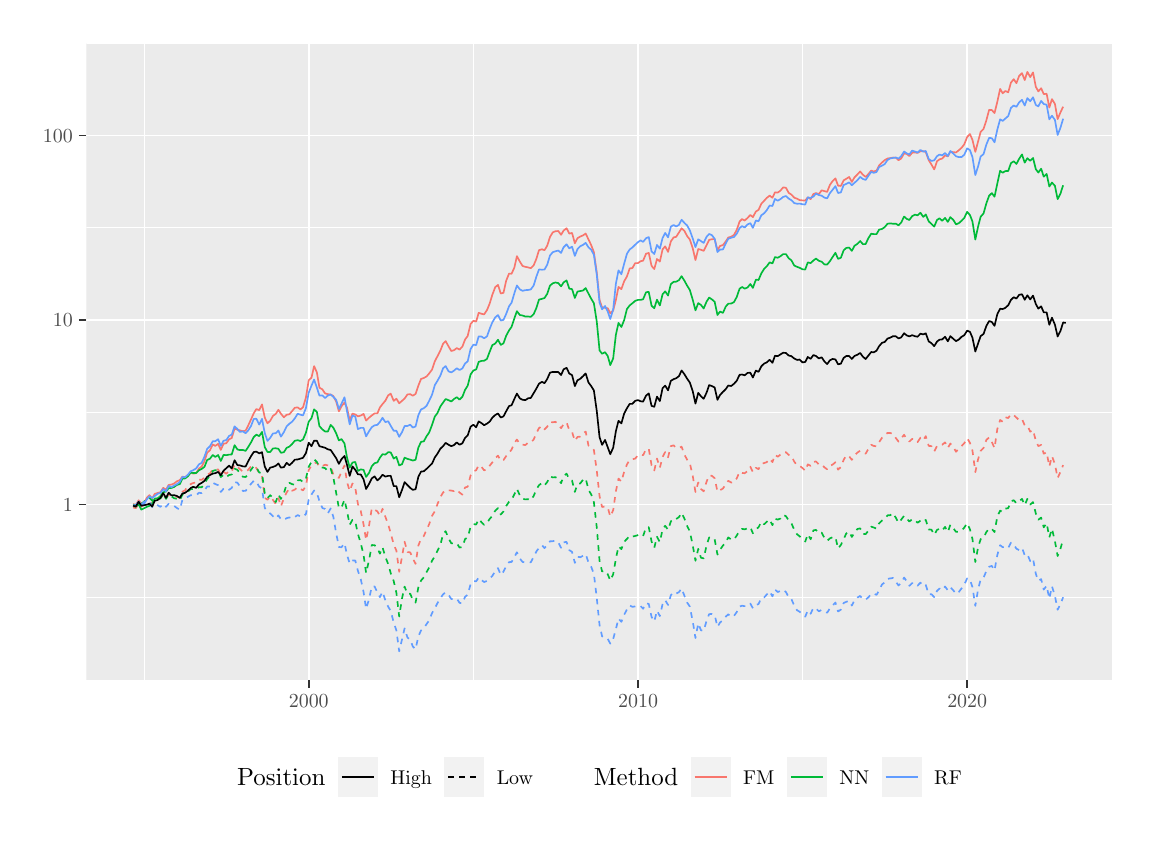
\begin{tikzpicture}[x=1pt,y=1pt]
\definecolor{fillColor}{RGB}{255,255,255}
\path[use as bounding box,fill=fillColor,fill opacity=0.00] (0,0) rectangle (397.48,289.08);
\begin{scope}
\path[clip] (  0.00,  0.00) rectangle (397.48,289.08);
\definecolor{drawColor}{RGB}{255,255,255}
\definecolor{fillColor}{RGB}{255,255,255}

\path[draw=drawColor,line width= 0.6pt,line join=round,line cap=round,fill=fillColor] (  0.00,  0.00) rectangle (397.48,289.08);
\end{scope}
\begin{scope}
\path[clip] ( 21.25, 53.26) rectangle (391.98,283.58);
\definecolor{fillColor}{gray}{0.92}

\path[fill=fillColor] ( 21.25, 53.26) rectangle (391.98,283.58);
\definecolor{drawColor}{RGB}{255,255,255}

\path[draw=drawColor,line width= 0.3pt,line join=round] ( 21.25, 83.37) --
	(391.98, 83.37);

\path[draw=drawColor,line width= 0.3pt,line join=round] ( 21.25,150.09) --
	(391.98,150.09);

\path[draw=drawColor,line width= 0.3pt,line join=round] ( 21.25,216.81) --
	(391.98,216.81);

\path[draw=drawColor,line width= 0.3pt,line join=round] ( 21.25,283.53) --
	(391.98,283.53);

\path[draw=drawColor,line width= 0.3pt,line join=round] ( 42.09, 53.26) --
	( 42.09,283.58);

\path[draw=drawColor,line width= 0.3pt,line join=round] (161.07, 53.26) --
	(161.07,283.58);

\path[draw=drawColor,line width= 0.3pt,line join=round] (280.03, 53.26) --
	(280.03,283.58);

\path[draw=drawColor,line width= 0.6pt,line join=round] ( 21.25,116.73) --
	(391.98,116.73);

\path[draw=drawColor,line width= 0.6pt,line join=round] ( 21.25,183.45) --
	(391.98,183.45);

\path[draw=drawColor,line width= 0.6pt,line join=round] ( 21.25,250.17) --
	(391.98,250.17);

\path[draw=drawColor,line width= 0.6pt,line join=round] (101.58, 53.26) --
	(101.58,283.58);

\path[draw=drawColor,line width= 0.6pt,line join=round] (220.56, 53.26) --
	(220.56,283.58);

\path[draw=drawColor,line width= 0.6pt,line join=round] (339.50, 53.26) --
	(339.50,283.58);
\definecolor{drawColor}{RGB}{248,118,109}

\path[draw=drawColor,line width= 0.6pt,line join=round] ( 38.10,116.96) --
	( 39.08,116.60) --
	( 40.09,118.30) --
	( 41.06,117.16) --
	( 42.04,117.41) --
	( 43.08,119.22) --
	( 43.99,120.15) --
	( 45.00,119.00) --
	( 45.92,120.62) --
	( 46.99,120.96) --
	( 47.97,121.21) --
	( 48.98,122.79) --
	( 49.99,122.10) --
	( 50.93,123.85) --
	( 51.97,123.98) --
	( 52.95,124.38) --
	( 53.90,125.16) --
	( 54.97,125.57) --
	( 55.91,126.84) --
	( 56.86,126.68) --
	( 57.90,127.37) --
	( 58.91,128.33) --
	( 59.82,127.92) --
	( 60.90,128.10) --
	( 61.88,129.76) --
	( 62.88,130.48) --
	( 63.89,132.43) --
	( 64.84,135.43) --
	( 65.88,136.41) --
	( 66.89,138.45) --
	( 67.80,137.96) --
	( 68.81,138.68) --
	( 69.79,136.49) --
	( 70.77,138.71) --
	( 71.78,138.93) --
	( 72.79,140.32) --
	( 73.73,140.79) --
	( 74.77,144.25) --
	( 75.78,143.79) --
	( 76.69,143.56) --
	( 77.77,143.27) --
	( 78.75,143.46) --
	( 79.66,145.26) --
	( 80.70,147.50) --
	( 81.68,149.72) --
	( 82.62,151.27) --
	( 83.66,150.88) --
	( 84.67,152.95) --
	( 85.68,148.16) --
	( 86.66,146.12) --
	( 87.64,147.04) --
	( 88.65,148.81) --
	( 89.66,149.53) --
	( 90.60,151.00) --
	( 91.51,149.57) --
	( 92.59,148.28) --
	( 93.57,149.19) --
	( 94.58,149.39) --
	( 95.55,150.53) --
	( 96.53,151.74) --
	( 97.57,151.86) --
	( 98.55,151.15) --
	( 99.49,151.89) --
	(100.54,155.41) --
	(101.55,161.65) --
	(102.56,162.63) --
	(103.50,166.78) --
	(104.51,164.49) --
	(105.42,158.99) --
	(106.50,158.38) --
	(107.47,156.92) --
	(108.48,156.65) --
	(109.49,156.51) --
	(110.44,155.98) --
	(111.48,153.95) --
	(112.46,150.45) --
	(113.40,152.28) --
	(114.48,153.60) --
	(115.39,151.71) --
	(116.36,147.15) --
	(117.37,149.64) --
	(118.38,149.31) --
	(119.33,148.64) --
	(120.37,148.92) --
	(121.38,149.51) --
	(122.29,147.11) --
	(123.37,148.14) --
	(124.34,148.96) --
	(125.35,149.70) --
	(126.36,149.69) --
	(127.28,151.84) --
	(128.22,153.07) --
	(129.26,154.29) --
	(130.27,156.24) --
	(131.18,156.83) --
	(132.26,154.23) --
	(133.24,155.00) --
	(134.25,153.35) --
	(135.26,154.23) --
	(136.20,155.07) --
	(137.24,156.55) --
	(138.25,156.64) --
	(139.16,156.09) --
	(140.17,156.72) --
	(141.15,159.65) --
	(142.13,162.13) --
	(143.14,162.51) --
	(144.15,163.04) --
	(145.09,164.16) --
	(146.13,165.54) --
	(147.14,168.56) --
	(148.06,170.32) --
	(149.13,172.40) --
	(150.11,174.88) --
	(151.02,175.82) --
	(152.09,173.90) --
	(153.07,172.24) --
	(154.08,172.54) --
	(155.06,173.30) --
	(156.04,172.75) --
	(157.08,173.83) --
	(158.05,176.38) --
	(159.00,177.69) --
	(160.04,182.00) --
	(161.05,183.15) --
	(162.06,182.90) --
	(162.97,186.03) --
	(163.98,185.69) --
	(164.93,185.47) --
	(165.97,187.02) --
	(166.95,189.40) --
	(167.89,192.52) --
	(168.97,195.36) --
	(169.94,196.11) --
	(170.95,193.03) --
	(171.93,193.28) --
	(172.91,197.67) --
	(173.95,200.22) --
	(174.86,200.17) --
	(175.87,202.40) --
	(176.78,206.52) --
	(177.86,204.53) --
	(178.83,202.96) --
	(179.84,202.64) --
	(180.85,202.45) --
	(181.80,202.17) --
	(182.84,203.19) --
	(183.82,205.57) --
	(184.76,208.68) --
	(185.84,209.00) --
	(186.75,208.66) --
	(187.73,210.28) --
	(188.74,213.46) --
	(189.74,215.11) --
	(190.69,215.52) --
	(191.73,215.59) --
	(192.74,214.24) --
	(193.65,215.76) --
	(194.73,216.59) --
	(195.71,214.67) --
	(196.71,214.90) --
	(197.72,211.18) --
	(198.67,213.00) --
	(199.68,213.61) --
	(200.66,214.00) --
	(201.63,214.70) --
	(202.64,212.57) --
	(203.65,210.45) --
	(204.60,207.94) --
	(205.64,200.64) --
	(206.65,190.64) --
	(207.56,188.02) --
	(208.64,187.82) --
	(209.61,187.70) --
	(210.52,185.86) --
	(211.57,186.89) --
	(212.54,190.65) --
	(213.49,195.38) --
	(214.53,194.60) --
	(215.54,197.45) --
	(216.55,199.18) --
	(217.53,202.08) --
	(218.50,202.20) --
	(219.51,203.98) --
	(220.52,204.00) --
	(221.47,204.68) --
	(222.38,204.88) --
	(223.45,207.40) --
	(224.43,207.68) --
	(225.44,203.02) --
	(226.42,201.84) --
	(227.40,205.49) --
	(228.44,204.55) --
	(229.42,208.97) --
	(230.36,210.06) --
	(231.40,208.04) --
	(232.41,211.85) --
	(233.42,213.29) --
	(234.33,213.50) --
	(235.34,215.07) --
	(236.29,216.58) --
	(237.33,215.63) --
	(238.31,213.73) --
	(239.25,212.56) --
	(240.33,209.31) --
	(241.30,205.10) --
	(242.31,209.09) --
	(243.29,208.81) --
	(244.27,208.44) --
	(245.31,210.45) --
	(246.25,212.41) --
	(247.23,212.62) --
	(248.24,212.70) --
	(249.25,208.66) --
	(250.19,210.21) --
	(251.24,210.52) --
	(252.25,211.82) --
	(253.16,213.24) --
	(254.23,213.54) --
	(255.21,214.19) --
	(256.22,216.02) --
	(257.23,218.99) --
	(258.14,219.91) --
	(259.09,219.38) --
	(260.13,220.33) --
	(261.14,221.41) --
	(262.05,220.62) --
	(263.13,222.64) --
	(264.10,223.24) --
	(265.11,225.46) --
	(266.12,226.53) --
	(267.07,227.58) --
	(268.11,228.38) --
	(269.12,227.61) --
	(270.03,229.58) --
	(271.04,229.49) --
	(272.02,230.21) --
	(272.99,231.37) --
	(274.00,231.22) --
	(275.01,229.37) --
	(275.96,228.77) --
	(277.00,227.64) --
	(278.01,227.28) --
	(278.92,226.79) --
	(280.00,226.66) --
	(280.97,226.58) --
	(281.89,227.79) --
	(282.93,227.10) --
	(283.90,228.96) --
	(284.85,229.31) --
	(285.89,228.94) --
	(286.90,230.30) --
	(287.91,230.02) --
	(288.89,229.74) --
	(289.87,232.24) --
	(290.87,233.65) --
	(291.88,234.60) --
	(292.83,231.99) --
	(293.84,231.89) --
	(294.85,233.91) --
	(295.79,234.47) --
	(296.84,235.12) --
	(297.81,233.34) --
	(298.76,234.98) --
	(299.83,236.05) --
	(300.81,237.12) --
	(301.82,235.92) --
	(302.80,235.16) --
	(303.77,236.17) --
	(304.81,237.44) --
	(305.73,237.08) --
	(306.74,237.46) --
	(307.65,239.28) --
	(308.72,240.35) --
	(309.70,241.22) --
	(310.71,241.80) --
	(311.72,241.95) --
	(312.66,242.14) --
	(313.71,242.09) --
	(314.68,241.19) --
	(315.63,241.80) --
	(316.70,243.67) --
	(317.61,243.45) --
	(318.59,242.67) --
	(319.60,243.89) --
	(320.61,243.97) --
	(321.56,243.84) --
	(322.60,244.43) --
	(323.61,244.48) --
	(324.52,244.14) --
	(325.59,241.20) --
	(326.57,239.63) --
	(327.58,237.86) --
	(328.59,240.81) --
	(329.50,241.50) --
	(330.45,241.78) --
	(331.49,242.90) --
	(332.50,242.56) --
	(333.41,244.25) --
	(334.49,244.08) --
	(335.46,243.99) --
	(336.47,244.79) --
	(337.48,245.70) --
	(338.43,246.93) --
	(339.47,249.56) --
	(340.48,250.65) --
	(341.39,248.53) --
	(342.43,244.19) --
	(343.41,247.88) --
	(344.35,251.43) --
	(345.40,252.47) --
	(346.41,255.58) --
	(347.42,259.39) --
	(348.39,259.31) --
	(349.37,258.22) --
	(350.38,262.31) --
	(351.39,266.96) --
	(352.33,265.37) --
	(353.25,266.19) --
	(354.32,265.73) --
	(355.30,269.22) --
	(356.31,270.47) --
	(357.28,269.03) --
	(358.26,271.63) --
	(359.30,272.65) --
	(360.28,270.14) --
	(361.23,273.11) --
	(362.27,271.22) --
	(363.28,272.92) --
	(364.29,267.70) --
	(365.20,266.06) --
	(366.21,267.19) --
	(367.15,265.10) --
	(368.20,265.19) --
	(369.17,260.21) --
	(370.12,263.27) --
	(371.19,261.53) --
	(372.17,256.02) --
	(373.18,258.44) --
	(374.16,260.52);

\path[draw=drawColor,line width= 0.6pt,dash pattern=on 2pt off 2pt ,line join=round] ( 38.10,115.73) --
	( 39.08,115.45) --
	( 40.09,117.08) --
	( 41.06,115.99) --
	( 42.04,116.90) --
	( 43.08,116.72) --
	( 43.99,117.04) --
	( 45.00,117.39) --
	( 45.92,119.07) --
	( 46.99,119.11) --
	( 47.97,119.22) --
	( 48.98,120.09) --
	( 49.99,119.01) --
	( 50.93,120.50) --
	( 51.97,119.90) --
	( 52.95,119.64) --
	( 53.90,119.58) --
	( 54.97,119.16) --
	( 55.91,121.41) --
	( 56.86,121.87) --
	( 57.90,123.54) --
	( 58.91,124.15) --
	( 59.82,124.55) --
	( 60.90,124.71) --
	( 61.88,125.80) --
	( 62.88,125.67) --
	( 63.89,126.50) --
	( 64.84,127.57) --
	( 65.88,128.04) --
	( 66.89,129.50) --
	( 67.80,129.20) --
	( 68.81,129.48) --
	( 69.79,127.70) --
	( 70.77,128.62) --
	( 71.78,127.88) --
	( 72.79,128.95) --
	( 73.73,128.68) --
	( 74.77,131.22) --
	( 75.78,130.36) --
	( 76.69,129.58) --
	( 77.77,128.61) --
	( 78.75,128.67) --
	( 79.66,129.26) --
	( 80.70,130.56) --
	( 81.68,130.82) --
	( 82.62,129.96) --
	( 83.66,128.12) --
	( 84.67,127.04) --
	( 85.68,119.15) --
	( 86.66,118.50) --
	( 87.64,119.74) --
	( 88.65,118.40) --
	( 89.66,116.94) --
	( 90.60,119.11) --
	( 91.51,116.11) --
	( 92.59,119.03) --
	( 93.57,121.13) --
	( 94.58,122.63) --
	( 95.55,121.74) --
	( 96.53,122.16) --
	( 97.57,123.04) --
	( 98.55,122.44) --
	( 99.49,121.86) --
	(100.54,123.51) --
	(101.55,129.19) --
	(102.56,130.91) --
	(103.50,131.62) --
	(104.51,132.02) --
	(105.42,130.39) --
	(106.50,130.66) --
	(107.47,131.14) --
	(108.48,130.90) --
	(109.49,130.48) --
	(110.44,127.63) --
	(111.48,126.89) --
	(112.46,126.39) --
	(113.40,128.65) --
	(114.48,130.90) --
	(115.39,124.93) --
	(116.36,121.69) --
	(117.37,124.38) --
	(118.38,122.80) --
	(119.33,116.98) --
	(120.37,114.38) --
	(121.38,109.54) --
	(122.29,103.93) --
	(123.37,109.23) --
	(124.34,115.43) --
	(125.35,114.89) --
	(126.36,114.30) --
	(127.28,112.67) --
	(128.22,115.22) --
	(129.26,112.32) --
	(130.27,109.59) --
	(131.18,106.42) --
	(132.26,102.37) --
	(133.24,100.09) --
	(134.25, 92.45) --
	(135.26, 97.84) --
	(136.20,103.32) --
	(137.24, 99.62) --
	(138.25, 99.46) --
	(139.16, 97.24) --
	(140.17, 95.33) --
	(141.15,101.88) --
	(142.13,104.38) --
	(143.14,105.37) --
	(144.15,107.71) --
	(145.09,109.67) --
	(146.13,112.70) --
	(147.14,114.36) --
	(148.06,116.87) --
	(149.13,119.45) --
	(150.11,121.11) --
	(151.02,122.01) --
	(152.09,121.91) --
	(153.07,121.81) --
	(154.08,121.59) --
	(155.06,122.15) --
	(156.04,121.12) --
	(157.08,120.34) --
	(158.05,122.93) --
	(159.00,123.20) --
	(160.04,127.26) --
	(161.05,128.79) --
	(162.06,129.15) --
	(162.97,130.99) --
	(163.98,130.39) --
	(164.93,129.12) --
	(165.97,129.49) --
	(166.95,130.80) --
	(167.89,131.97) --
	(168.97,133.52) --
	(169.94,134.43) --
	(170.95,132.54) --
	(171.93,132.84) --
	(172.91,134.27) --
	(173.95,135.45) --
	(174.86,136.64) --
	(175.87,138.99) --
	(176.78,140.25) --
	(177.86,138.60) --
	(178.83,138.37) --
	(179.84,138.27) --
	(180.85,139.14) --
	(181.80,139.14) --
	(182.84,140.25) --
	(183.82,142.58) --
	(184.76,144.38) --
	(185.84,145.12) --
	(186.75,143.93) --
	(187.73,144.90) --
	(188.74,146.63) --
	(189.74,146.49) --
	(190.69,146.66) --
	(191.73,145.76) --
	(192.74,144.35) --
	(193.65,145.81) --
	(194.73,146.47) --
	(195.71,143.65) --
	(196.71,143.00) --
	(197.72,139.76) --
	(198.67,141.19) --
	(199.68,141.31) --
	(200.66,142.49) --
	(201.63,143.12) --
	(202.64,138.08) --
	(203.65,137.57) --
	(204.60,136.45) --
	(205.64,129.09) --
	(206.65,119.73) --
	(207.56,115.89) --
	(208.64,116.08) --
	(209.61,115.72) --
	(210.52,112.43) --
	(211.57,114.72) --
	(212.54,121.49) --
	(213.49,126.15) --
	(214.53,125.02) --
	(215.54,128.64) --
	(216.55,131.25) --
	(217.53,132.93) --
	(218.50,133.13) --
	(219.51,133.35) --
	(220.52,134.54) --
	(221.47,134.87) --
	(222.38,134.58) --
	(223.45,136.77) --
	(224.43,136.95) --
	(225.44,130.97) --
	(226.42,129.06) --
	(227.40,133.39) --
	(228.44,130.08) --
	(229.42,133.96) --
	(230.36,135.72) --
	(231.40,133.84) --
	(232.41,137.86) --
	(233.42,138.16) --
	(234.33,137.23) --
	(235.34,137.21) --
	(236.29,137.67) --
	(237.33,134.76) --
	(238.31,132.92) --
	(239.25,131.82) --
	(240.33,127.06) --
	(241.30,121.29) --
	(242.31,124.73) --
	(243.29,122.39) --
	(244.27,121.54) --
	(245.31,125.00) --
	(246.25,127.29) --
	(247.23,127.14) --
	(248.24,126.30) --
	(249.25,121.42) --
	(250.19,121.96) --
	(251.24,122.55) --
	(252.25,124.11) --
	(253.16,125.34) --
	(254.23,124.72) --
	(255.21,124.83) --
	(256.22,126.21) --
	(257.23,128.60) --
	(258.14,128.17) --
	(259.09,128.08) --
	(260.13,128.87) --
	(261.14,130.41) --
	(262.05,128.46) --
	(263.13,130.06) --
	(264.10,129.55) --
	(265.11,131.52) --
	(266.12,131.75) --
	(267.07,132.09) --
	(268.11,133.34) --
	(269.12,132.10) --
	(270.03,134.72) --
	(271.04,134.03) --
	(272.02,134.82) --
	(272.99,135.68) --
	(274.00,135.63) --
	(275.01,134.69) --
	(275.96,134.37) --
	(277.00,132.26) --
	(278.01,130.95) --
	(278.92,130.76) --
	(280.00,129.94) --
	(280.97,128.98) --
	(281.89,131.26) --
	(282.93,130.74) --
	(283.90,132.19) --
	(284.85,132.33) --
	(285.89,131.24) --
	(286.90,131.28) --
	(287.91,130.20) --
	(288.89,129.49) --
	(289.87,130.75) --
	(290.87,131.20) --
	(291.88,132.04) --
	(292.83,129.38) --
	(293.84,130.30) --
	(294.85,132.90) --
	(295.79,134.54) --
	(296.84,134.18) --
	(297.81,132.91) --
	(298.76,134.53) --
	(299.83,135.54) --
	(300.81,136.21) --
	(301.82,135.60) --
	(302.80,135.13) --
	(303.77,136.85) --
	(304.81,138.37) --
	(305.73,137.93) --
	(306.74,137.80) --
	(307.65,139.26) --
	(308.72,140.91) --
	(309.70,141.78) --
	(310.71,142.65) --
	(311.72,142.60) --
	(312.66,142.31) --
	(313.71,140.80) --
	(314.68,139.51) --
	(315.63,140.61) --
	(316.70,141.98) --
	(317.61,140.34) --
	(318.59,139.51) --
	(319.60,140.46) --
	(320.61,140.33) --
	(321.56,139.31) --
	(322.60,140.90) --
	(323.61,140.00) --
	(324.52,141.48) --
	(325.59,137.96) --
	(326.57,137.87) --
	(327.58,135.95) --
	(328.59,137.96) --
	(329.50,138.32) --
	(330.45,138.38) --
	(331.49,139.21) --
	(332.50,137.21) --
	(333.41,138.80) --
	(334.49,137.58) --
	(335.46,135.83) --
	(336.47,137.04) --
	(337.48,137.93) --
	(338.43,138.91) --
	(339.47,140.73) --
	(340.48,139.09) --
	(341.39,136.28) --
	(342.43,128.48) --
	(343.41,133.06) --
	(344.35,136.14) --
	(345.40,137.20) --
	(346.41,140.10) --
	(347.42,141.03) --
	(348.39,139.40) --
	(349.37,137.12) --
	(350.38,144.06) --
	(351.39,147.33) --
	(352.33,146.67) --
	(353.25,148.30) --
	(354.32,148.02) --
	(355.30,149.40) --
	(356.31,149.07) --
	(357.28,148.18) --
	(358.26,147.25) --
	(359.30,147.66) --
	(360.28,145.36) --
	(361.23,145.31) --
	(362.27,143.09) --
	(363.28,143.71) --
	(364.29,139.78) --
	(365.20,137.88) --
	(366.21,138.30) --
	(367.15,135.12) --
	(368.20,135.64) --
	(369.17,130.50) --
	(370.12,134.27) --
	(371.19,131.36) --
	(372.17,126.33) --
	(373.18,128.55) --
	(374.16,131.01);
\definecolor{drawColor}{RGB}{0,186,56}

\path[draw=drawColor,line width= 0.6pt,line join=round] ( 38.10,116.22) --
	( 39.08,116.02) --
	( 40.09,116.88) --
	( 41.06,114.91) --
	( 42.04,115.40) --
	( 43.08,115.93) --
	( 43.99,116.30) --
	( 45.00,117.09) --
	( 45.92,118.91) --
	( 46.99,119.04) --
	( 47.97,119.84) --
	( 48.98,121.19) --
	( 49.99,121.49) --
	( 50.93,122.66) --
	( 51.97,122.78) --
	( 52.95,123.12) --
	( 53.90,123.86) --
	( 54.97,124.14) --
	( 55.91,126.09) --
	( 56.86,126.19) --
	( 57.90,126.95) --
	( 58.91,128.33) --
	( 59.82,128.16) --
	( 60.90,128.16) --
	( 61.88,129.12) --
	( 62.88,129.64) --
	( 63.89,130.38) --
	( 64.84,132.84) --
	( 65.88,133.35) --
	( 66.89,134.66) --
	( 67.80,133.97) --
	( 68.81,134.66) --
	( 69.79,132.49) --
	( 70.77,134.68) --
	( 71.78,134.61) --
	( 72.79,134.80) --
	( 73.73,134.84) --
	( 74.77,138.21) --
	( 75.78,136.67) --
	( 76.69,136.45) --
	( 77.77,136.48) --
	( 78.75,136.16) --
	( 79.66,137.51) --
	( 80.70,139.22) --
	( 81.68,141.12) --
	( 82.62,142.02) --
	( 83.66,141.48) --
	( 84.67,143.00) --
	( 85.68,137.51) --
	( 86.66,135.74) --
	( 87.64,135.75) --
	( 88.65,137.05) --
	( 89.66,137.09) --
	( 90.60,136.91) --
	( 91.51,135.47) --
	( 92.59,135.67) --
	( 93.57,137.26) --
	( 94.58,137.69) --
	( 95.55,138.64) --
	( 96.53,139.81) --
	( 97.57,140.02) --
	( 98.55,139.71) --
	( 99.49,140.28) --
	(100.54,142.70) --
	(101.55,146.70) --
	(102.56,148.01) --
	(103.50,151.17) --
	(104.51,150.19) --
	(105.42,145.10) --
	(106.50,143.91) --
	(107.47,143.15) --
	(108.48,143.14) --
	(109.49,145.55) --
	(110.44,144.53) --
	(111.48,142.48) --
	(112.46,139.92) --
	(113.40,140.43) --
	(114.48,138.83) --
	(115.39,133.74) --
	(116.36,130.14) --
	(117.37,131.94) --
	(118.38,132.14) --
	(119.33,128.92) --
	(120.37,129.46) --
	(121.38,129.29) --
	(122.29,126.74) --
	(123.37,128.23) --
	(124.34,130.60) --
	(125.35,131.71) --
	(126.36,131.99) --
	(127.28,133.68) --
	(128.22,134.95) --
	(129.26,134.81) --
	(130.27,135.68) --
	(131.18,135.61) --
	(132.26,133.38) --
	(133.24,133.97) --
	(134.25,130.90) --
	(135.26,131.33) --
	(136.20,133.68) --
	(137.24,133.26) --
	(138.25,132.98) --
	(139.16,132.66) --
	(140.17,132.93) --
	(141.15,137.28) --
	(142.13,139.40) --
	(143.14,139.60) --
	(144.15,141.46) --
	(145.09,142.83) --
	(146.13,145.58) --
	(147.14,148.58) --
	(148.06,149.80) --
	(149.13,152.22) --
	(150.11,153.61) --
	(151.02,154.89) --
	(152.09,154.47) --
	(153.07,154.00) --
	(154.08,154.92) --
	(155.06,155.55) --
	(156.04,154.67) --
	(157.08,155.71) --
	(158.05,158.19) --
	(159.00,159.72) --
	(160.04,163.76) --
	(161.05,165.19) --
	(162.06,165.60) --
	(162.97,168.33) --
	(163.98,168.67) --
	(164.93,168.72) --
	(165.97,169.39) --
	(166.95,172.01) --
	(167.89,174.35) --
	(168.97,174.95) --
	(169.94,176.30) --
	(170.95,174.46) --
	(171.93,175.01) --
	(172.91,177.78) --
	(173.95,179.70) --
	(174.86,180.99) --
	(175.87,184.06) --
	(176.78,186.62) --
	(177.86,185.25) --
	(178.83,185.07) --
	(179.84,184.69) --
	(180.85,184.70) --
	(181.80,184.59) --
	(182.84,185.56) --
	(183.82,187.78) --
	(184.76,190.82) --
	(185.84,191.09) --
	(186.75,191.38) --
	(187.73,192.88) --
	(188.74,195.88) --
	(189.74,196.71) --
	(190.69,196.99) --
	(191.73,196.79) --
	(192.74,195.59) --
	(193.65,197.02) --
	(194.73,197.76) --
	(195.71,194.77) --
	(196.71,194.60) --
	(197.72,191.41) --
	(198.67,193.71) --
	(199.68,193.91) --
	(200.66,194.08) --
	(201.63,194.99) --
	(202.64,193.00) --
	(203.65,191.09) --
	(204.60,189.50) --
	(205.64,182.85) --
	(206.65,172.46) --
	(207.56,171.25) --
	(208.64,171.82) --
	(209.61,170.41) --
	(210.52,167.14) --
	(211.57,169.56) --
	(212.54,178.08) --
	(213.49,182.37) --
	(214.53,180.92) --
	(215.54,183.42) --
	(216.55,187.43) --
	(217.53,188.71) --
	(218.50,189.48) --
	(219.51,190.36) --
	(220.52,190.70) --
	(221.47,190.71) --
	(222.38,190.94) --
	(223.45,193.48) --
	(224.43,193.60) --
	(225.44,188.59) --
	(226.42,187.70) --
	(227.40,190.79) --
	(228.44,188.71) --
	(229.42,192.74) --
	(230.36,193.79) --
	(231.40,192.29) --
	(232.41,196.43) --
	(233.42,197.24) --
	(234.33,197.30) --
	(235.34,197.84) --
	(236.29,199.28) --
	(237.33,197.62) --
	(238.31,195.82) --
	(239.25,194.33) --
	(240.33,190.73) --
	(241.30,186.93) --
	(242.31,189.54) --
	(243.29,188.88) --
	(244.27,187.62) --
	(245.31,190.07) --
	(246.25,191.55) --
	(247.23,190.91) --
	(248.24,190.02) --
	(249.25,185.26) --
	(250.19,186.49) --
	(251.24,186.03) --
	(252.25,188.31) --
	(253.16,189.33) --
	(254.23,189.40) --
	(255.21,189.90) --
	(256.22,191.76) --
	(257.23,194.72) --
	(258.14,195.39) --
	(259.09,194.77) --
	(260.13,195.20) --
	(261.14,196.45) --
	(262.05,195.04) --
	(263.13,198.01) --
	(264.10,197.91) --
	(265.11,200.31) --
	(266.12,201.92) --
	(267.07,202.85) --
	(268.11,204.27) --
	(269.12,203.89) --
	(270.03,206.18) --
	(271.04,205.94) --
	(272.02,206.50) --
	(272.99,207.25) --
	(274.00,207.24) --
	(275.01,205.74) --
	(275.96,205.02) --
	(277.00,203.12) --
	(278.01,202.66) --
	(278.92,202.32) --
	(280.00,201.75) --
	(280.97,201.71) --
	(281.89,204.25) --
	(282.93,204.01) --
	(283.90,204.93) --
	(284.85,205.64) --
	(285.89,204.84) --
	(286.90,204.50) --
	(287.91,203.53) --
	(288.89,203.49) --
	(289.87,204.67) --
	(290.87,206.22) --
	(291.88,207.72) --
	(292.83,205.54) --
	(293.84,205.92) --
	(294.85,208.63) --
	(295.79,209.48) --
	(296.84,209.62) --
	(297.81,208.42) --
	(298.76,210.24) --
	(299.83,210.97) --
	(300.81,211.98) --
	(301.82,210.84) --
	(302.80,210.89) --
	(303.77,213.00) --
	(304.81,214.61) --
	(305.73,214.48) --
	(306.74,214.47) --
	(307.65,216.09) --
	(308.72,216.34) --
	(309.70,217.02) --
	(310.71,218.23) --
	(311.72,218.36) --
	(312.66,218.23) --
	(313.71,218.25) --
	(314.68,217.66) --
	(315.63,218.64) --
	(316.70,220.82) --
	(317.61,220.01) --
	(318.59,219.58) --
	(319.60,220.97) --
	(320.61,221.50) --
	(321.56,221.28) --
	(322.60,222.20) --
	(323.61,220.70) --
	(324.52,221.58) --
	(325.59,219.10) --
	(326.57,218.14) --
	(327.58,217.20) --
	(328.59,219.62) --
	(329.50,220.19) --
	(330.45,219.30) --
	(331.49,220.34) --
	(332.50,218.90) --
	(333.41,220.62) --
	(334.49,219.59) --
	(335.46,218.01) --
	(336.47,218.43) --
	(337.48,219.32) --
	(338.43,220.32) --
	(339.47,222.52) --
	(340.48,221.40) --
	(341.39,219.05) --
	(342.43,212.52) --
	(343.41,217.13) --
	(344.35,220.74) --
	(345.40,221.95) --
	(346.41,225.58) --
	(347.42,228.36) --
	(348.39,229.29) --
	(349.37,227.99) --
	(350.38,232.77) --
	(351.39,237.37) --
	(352.33,236.67) --
	(353.25,237.25) --
	(354.32,237.30) --
	(355.30,240.12) --
	(356.31,240.79) --
	(357.28,239.82) --
	(358.26,241.68) --
	(359.30,243.28) --
	(360.28,240.30) --
	(361.23,241.91) --
	(362.27,240.98) --
	(363.28,241.97) --
	(364.29,237.93) --
	(365.20,236.72) --
	(366.21,238.12) --
	(367.15,235.24) --
	(368.20,236.22) --
	(369.17,231.67) --
	(370.12,233.11) --
	(371.19,231.93) --
	(372.17,227.12) --
	(373.18,229.10) --
	(374.16,232.12);

\path[draw=drawColor,line width= 0.6pt,dash pattern=on 2pt off 2pt ,line join=round] ( 38.10,116.73) --
	( 39.08,116.32) --
	( 40.09,117.91) --
	( 41.06,117.01) --
	( 42.04,117.79) --
	( 43.08,118.95) --
	( 43.99,119.18) --
	( 45.00,118.13) --
	( 45.92,118.98) --
	( 46.99,119.04) --
	( 47.97,118.92) --
	( 48.98,120.60) --
	( 49.99,118.81) --
	( 50.93,120.38) --
	( 51.97,119.71) --
	( 52.95,119.02) --
	( 53.90,118.84) --
	( 54.97,118.22) --
	( 55.91,120.33) --
	( 56.86,120.79) --
	( 57.90,121.45) --
	( 58.91,122.32) --
	( 59.82,122.34) --
	( 60.90,122.27) --
	( 61.88,123.03) --
	( 62.88,123.01) --
	( 63.89,124.28) --
	( 64.84,125.96) --
	( 65.88,127.14) --
	( 66.89,128.90) --
	( 67.80,129.19) --
	( 68.81,128.89) --
	( 69.79,126.70) --
	( 70.77,127.48) --
	( 71.78,126.68) --
	( 72.79,127.44) --
	( 73.73,127.63) --
	( 74.77,129.72) --
	( 75.78,129.29) --
	( 76.69,128.15) --
	( 77.77,126.79) --
	( 78.75,126.72) --
	( 79.66,127.58) --
	( 80.70,129.32) --
	( 81.68,130.64) --
	( 82.62,130.25) --
	( 83.66,128.35) --
	( 84.67,128.11) --
	( 85.68,120.83) --
	( 86.66,119.08) --
	( 87.64,120.14) --
	( 88.65,119.19) --
	( 89.66,117.64) --
	( 90.60,120.42) --
	( 91.51,118.78) --
	( 92.59,120.84) --
	( 93.57,124.11) --
	( 94.58,124.59) --
	( 95.55,124.11) --
	( 96.53,123.94) --
	( 97.57,125.48) --
	( 98.55,125.61) --
	( 99.49,124.90) --
	(100.54,126.15) --
	(101.55,130.44) --
	(102.56,132.18) --
	(103.50,133.14) --
	(104.51,132.11) --
	(105.42,130.36) --
	(106.50,130.12) --
	(107.47,129.92) --
	(108.48,128.81) --
	(109.49,129.71) --
	(110.44,126.60) --
	(111.48,120.93) --
	(112.46,115.50) --
	(113.40,115.69) --
	(114.48,118.50) --
	(115.39,114.39) --
	(116.36,109.42) --
	(117.37,111.25) --
	(118.38,110.61) --
	(119.33,106.15) --
	(120.37,102.73) --
	(121.38, 98.56) --
	(122.29, 92.01) --
	(123.37, 96.74) --
	(124.34,102.13) --
	(125.35,102.07) --
	(126.36,101.00) --
	(127.28, 99.02) --
	(128.22,101.34) --
	(129.26, 97.80) --
	(130.27, 95.27) --
	(131.18, 91.98) --
	(132.26, 89.12) --
	(133.24, 84.84) --
	(134.25, 76.30) --
	(135.26, 82.81) --
	(136.20, 87.11) --
	(137.24, 84.44) --
	(138.25, 84.52) --
	(139.16, 82.28) --
	(140.17, 81.33) --
	(141.15, 86.78) --
	(142.13, 89.28) --
	(143.14, 90.46) --
	(144.15, 92.35) --
	(145.09, 94.04) --
	(146.13, 96.49) --
	(147.14, 98.04) --
	(148.06,100.00) --
	(149.13,102.23) --
	(150.11,106.04) --
	(151.02,107.13) --
	(152.09,104.50) --
	(153.07,102.78) --
	(154.08,102.67) --
	(155.06,102.81) --
	(156.04,101.24) --
	(157.08,101.41) --
	(158.05,104.30) --
	(159.00,104.84) --
	(160.04,108.71) --
	(161.05,109.72) --
	(162.06,109.54) --
	(162.97,111.51) --
	(163.98,110.39) --
	(164.93,109.43) --
	(165.97,110.05) --
	(166.95,111.59) --
	(167.89,112.62) --
	(168.97,114.57) --
	(169.94,115.44) --
	(170.95,113.17) --
	(171.93,114.27) --
	(172.91,116.22) --
	(173.95,117.81) --
	(174.86,118.48) --
	(175.87,120.46) --
	(176.78,122.48) --
	(177.86,120.00) --
	(178.83,118.86) --
	(179.84,118.62) --
	(180.85,118.69) --
	(181.80,118.29) --
	(182.84,119.88) --
	(183.82,122.24) --
	(184.76,123.74) --
	(185.84,124.58) --
	(186.75,123.68) --
	(187.73,124.89) --
	(188.74,126.97) --
	(189.74,126.56) --
	(190.69,126.64) --
	(191.73,126.10) --
	(192.74,124.46) --
	(193.65,127.05) --
	(194.73,127.91) --
	(195.71,125.88) --
	(196.71,125.42) --
	(197.72,121.32) --
	(198.67,124.16) --
	(199.68,124.40) --
	(200.66,125.70) --
	(201.63,126.25) --
	(202.64,122.08) --
	(203.65,120.39) --
	(204.60,117.63) --
	(205.64,108.51) --
	(206.65, 96.40) --
	(207.56, 92.59) --
	(208.64, 92.81) --
	(209.61, 91.56) --
	(210.52, 89.31) --
	(211.57, 91.56) --
	(212.54, 97.11) --
	(213.49,101.69) --
	(214.53,100.65) --
	(215.54,103.31) --
	(216.55,104.33) --
	(217.53,105.53) --
	(218.50,105.19) --
	(219.51,105.40) --
	(220.52,105.73) --
	(221.47,105.98) --
	(222.38,105.39) --
	(223.45,108.43) --
	(224.43,108.58) --
	(225.44,103.41) --
	(226.42,101.13) --
	(227.40,105.13) --
	(228.44,103.16) --
	(229.42,107.86) --
	(230.36,109.07) --
	(231.40,107.63) --
	(232.41,110.69) --
	(233.42,111.70) --
	(234.33,111.51) --
	(235.34,112.24) --
	(236.29,113.78) --
	(237.33,111.62) --
	(238.31,109.00) --
	(239.25,107.13) --
	(240.33,101.98) --
	(241.30, 96.46) --
	(242.31,100.74) --
	(243.29, 97.55) --
	(244.27, 97.31) --
	(245.31,101.97) --
	(246.25,104.88) --
	(247.23,104.20) --
	(248.24,104.21) --
	(249.25, 98.67) --
	(250.19,100.44) --
	(251.24,101.96) --
	(252.25,103.08) --
	(253.16,104.87) --
	(254.23,104.12) --
	(255.21,104.07) --
	(256.22,105.57) --
	(257.23,107.36) --
	(258.14,107.98) --
	(259.09,107.78) --
	(260.13,108.20) --
	(261.14,108.56) --
	(262.05,106.39) --
	(263.13,107.75) --
	(264.10,108.56) --
	(265.11,110.55) --
	(266.12,109.62) --
	(267.07,110.54) --
	(268.11,111.38) --
	(269.12,109.32) --
	(270.03,111.62) --
	(271.04,111.33) --
	(272.02,111.71) --
	(272.99,113.04) --
	(274.00,112.56) --
	(275.01,111.00) --
	(275.96,110.03) --
	(277.00,107.63) --
	(278.01,106.02) --
	(278.92,105.31) --
	(280.00,104.29) --
	(280.97,103.40) --
	(281.89,106.02) --
	(282.93,104.23) --
	(283.90,107.42) --
	(284.85,107.60) --
	(285.89,106.37) --
	(286.90,106.60) --
	(287.91,104.70) --
	(288.89,103.64) --
	(289.87,104.53) --
	(290.87,104.94) --
	(291.88,105.01) --
	(292.83,100.86) --
	(293.84,102.16) --
	(294.85,104.21) --
	(295.79,106.32) --
	(296.84,106.96) --
	(297.81,105.05) --
	(298.76,106.59) --
	(299.83,107.94) --
	(300.81,108.15) --
	(301.82,106.11) --
	(302.80,106.08) --
	(303.77,107.29) --
	(304.81,108.76) --
	(305.73,108.47) --
	(306.74,108.04) --
	(307.65,109.94) --
	(308.72,110.98) --
	(309.70,111.56) --
	(310.71,112.86) --
	(311.72,112.92) --
	(312.66,113.67) --
	(313.71,111.99) --
	(314.68,110.16) --
	(315.63,111.28) --
	(316.70,112.71) --
	(317.61,111.76) --
	(318.59,110.62) --
	(319.60,111.45) --
	(320.61,111.20) --
	(321.56,110.16) --
	(322.60,110.97) --
	(323.61,110.38) --
	(324.52,111.21) --
	(325.59,107.72) --
	(326.57,107.71) --
	(327.58,105.81) --
	(328.59,107.61) --
	(329.50,108.00) --
	(330.45,107.34) --
	(331.49,108.70) --
	(332.50,106.82) --
	(333.41,109.46) --
	(334.49,108.21) --
	(335.46,106.87) --
	(336.47,107.01) --
	(337.48,107.37) --
	(338.43,108.42) --
	(339.47,110.05) --
	(340.48,107.83) --
	(341.39,104.35) --
	(342.43, 96.01) --
	(343.41,101.21) --
	(344.35,104.25) --
	(345.40,104.73) --
	(346.41,106.79) --
	(347.42,108.12) --
	(348.39,107.98) --
	(349.37,106.81) --
	(350.38,112.44) --
	(351.39,114.55) --
	(352.33,114.06) --
	(353.25,115.27) --
	(354.32,115.45) --
	(355.30,117.90) --
	(356.31,118.32) --
	(357.28,117.23) --
	(358.26,118.01) --
	(359.30,118.78) --
	(360.28,116.53) --
	(361.23,118.82) --
	(362.27,116.77) --
	(363.28,117.65) --
	(364.29,113.53) --
	(365.20,111.30) --
	(366.21,112.05) --
	(367.15,108.53) --
	(368.20,110.05) --
	(369.17,104.91) --
	(370.12,108.01) --
	(371.19,103.54) --
	(372.17, 98.17) --
	(373.18,100.75) --
	(374.16,104.21);
\definecolor{drawColor}{RGB}{97,156,255}

\path[draw=drawColor,line width= 0.6pt,line join=round] ( 38.10,116.18) --
	( 39.08,116.20) --
	( 40.09,117.85) --
	( 41.06,116.49) --
	( 42.04,116.86) --
	( 43.08,118.67) --
	( 43.99,119.74) --
	( 45.00,119.13) --
	( 45.92,119.84) --
	( 46.99,120.67) --
	( 47.97,120.98) --
	( 48.98,122.35) --
	( 49.99,121.52) --
	( 50.93,123.50) --
	( 51.97,123.07) --
	( 52.95,123.62) --
	( 53.90,124.11) --
	( 54.97,124.92) --
	( 55.91,126.73) --
	( 56.86,126.60) --
	( 57.90,127.53) --
	( 58.91,128.80) --
	( 59.82,129.16) --
	( 60.90,129.85) --
	( 61.88,131.27) --
	( 62.88,131.84) --
	( 63.89,134.08) --
	( 64.84,136.86) --
	( 65.88,137.85) --
	( 66.89,139.66) --
	( 67.80,139.65) --
	( 68.81,140.37) --
	( 69.79,137.96) --
	( 70.77,139.81) --
	( 71.78,140.05) --
	( 72.79,141.58) --
	( 73.73,142.00) --
	( 74.77,145.02) --
	( 75.78,144.05) --
	( 76.69,143.02) --
	( 77.77,143.18) --
	( 78.75,142.53) --
	( 79.66,143.52) --
	( 80.70,145.13) --
	( 81.68,147.67) --
	( 82.62,147.78) --
	( 83.66,145.66) --
	( 84.67,147.72) --
	( 85.68,142.55) --
	( 86.66,139.76) --
	( 87.64,140.86) --
	( 88.65,142.47) --
	( 89.66,142.52) --
	( 90.60,143.52) --
	( 91.51,141.29) --
	( 92.59,142.94) --
	( 93.57,145.01) --
	( 94.58,145.96) --
	( 95.55,146.70) --
	( 96.53,147.90) --
	( 97.57,149.57) --
	( 98.55,149.22) --
	( 99.49,148.98) --
	(100.54,151.60) --
	(101.55,157.19) --
	(102.56,159.74) --
	(103.50,161.92) --
	(104.51,158.98) --
	(105.42,156.14) --
	(106.50,156.17) --
	(107.47,155.24) --
	(108.48,156.17) --
	(109.49,156.52) --
	(110.44,155.67) --
	(111.48,154.58) --
	(112.46,151.31) --
	(113.40,153.20) --
	(114.48,155.52) --
	(115.39,150.53) --
	(116.36,145.72) --
	(117.37,148.93) --
	(118.38,148.53) --
	(119.33,144.03) --
	(120.37,144.48) --
	(121.38,144.44) --
	(122.29,141.38) --
	(123.37,143.29) --
	(124.34,144.70) --
	(125.35,145.38) --
	(126.36,145.56) --
	(127.28,146.62) --
	(128.22,148.11) --
	(129.26,146.55) --
	(130.27,146.85) --
	(131.18,145.23) --
	(132.26,143.44) --
	(133.24,143.43) --
	(134.25,141.22) --
	(135.26,142.91) --
	(136.20,145.13) --
	(137.24,145.17) --
	(138.25,145.61) --
	(139.16,144.60) --
	(140.17,144.97) --
	(141.15,148.99) --
	(142.13,151.13) --
	(143.14,151.57) --
	(144.15,152.43) --
	(145.09,154.27) --
	(146.13,156.47) --
	(147.14,159.94) --
	(148.06,161.45) --
	(149.13,163.37) --
	(150.11,166.02) --
	(151.02,166.79) --
	(152.09,164.88) --
	(153.07,164.51) --
	(154.08,165.17) --
	(155.06,166.00) --
	(156.04,165.37) --
	(157.08,165.94) --
	(158.05,167.73) --
	(159.00,168.51) --
	(160.04,172.95) --
	(161.05,174.52) --
	(162.06,174.37) --
	(162.97,177.53) --
	(163.98,177.47) --
	(164.93,176.84) --
	(165.97,177.53) --
	(166.95,180.25) --
	(167.89,182.58) --
	(168.97,184.42) --
	(169.94,185.23) --
	(170.95,183.25) --
	(171.93,183.50) --
	(172.91,185.65) --
	(173.95,188.43) --
	(174.86,189.71) --
	(175.87,193.13) --
	(176.78,195.93) --
	(177.86,194.50) --
	(178.83,193.99) --
	(179.84,194.24) --
	(180.85,194.30) --
	(181.80,194.49) --
	(182.84,195.93) --
	(183.82,199.12) --
	(184.76,201.70) --
	(185.84,201.62) --
	(186.75,201.68) --
	(187.73,203.40) --
	(188.74,206.76) --
	(189.74,207.96) --
	(190.69,208.27) --
	(191.73,208.54) --
	(192.74,207.69) --
	(193.65,209.73) --
	(194.73,210.80) --
	(195.71,209.34) --
	(196.71,209.94) --
	(197.72,206.60) --
	(198.67,209.06) --
	(199.68,210.10) --
	(200.66,210.59) --
	(201.63,211.31) --
	(202.64,209.71) --
	(203.65,208.83) --
	(204.60,206.99) --
	(205.64,199.81) --
	(206.65,189.70) --
	(207.56,187.31) --
	(208.64,188.50) --
	(209.61,186.50) --
	(210.52,183.82) --
	(211.57,187.23) --
	(212.54,196.48) --
	(213.49,201.38) --
	(214.53,199.99) --
	(215.54,203.80) --
	(216.55,207.40) --
	(217.53,208.91) --
	(218.50,209.66) --
	(219.51,210.63) --
	(220.52,211.57) --
	(221.47,212.21) --
	(222.38,211.68) --
	(223.45,212.99) --
	(224.43,213.42) --
	(225.44,208.23) --
	(226.42,207.28) --
	(227.40,210.57) --
	(228.44,209.22) --
	(229.42,213.09) --
	(230.36,214.90) --
	(231.40,213.32) --
	(232.41,217.19) --
	(233.42,217.78) --
	(234.33,217.22) --
	(235.34,217.83) --
	(236.29,219.67) --
	(237.33,218.51) --
	(238.31,217.57) --
	(239.25,215.89) --
	(240.33,212.86) --
	(241.30,209.79) --
	(242.31,212.61) --
	(243.29,211.97) --
	(244.27,211.31) --
	(245.31,213.50) --
	(246.25,214.53) --
	(247.23,214.12) --
	(248.24,212.77) --
	(249.25,208.00) --
	(250.19,208.89) --
	(251.24,208.96) --
	(252.25,211.11) --
	(253.16,212.82) --
	(254.23,213.18) --
	(255.21,213.43) --
	(256.22,214.64) --
	(257.23,216.66) --
	(258.14,217.36) --
	(259.09,216.89) --
	(260.13,217.97) --
	(261.14,218.44) --
	(262.05,216.73) --
	(263.13,219.40) --
	(264.10,219.13) --
	(265.11,221.30) --
	(266.12,222.00) --
	(267.07,223.14) --
	(268.11,224.82) --
	(269.12,224.64) --
	(270.03,227.17) --
	(271.04,226.56) --
	(272.02,227.13) --
	(272.99,227.91) --
	(274.00,228.24) --
	(275.01,227.31) --
	(275.96,226.75) --
	(277.00,225.69) --
	(278.01,225.45) --
	(278.92,225.51) --
	(280.00,225.26) --
	(280.97,225.18) --
	(281.89,227.74) --
	(282.93,227.56) --
	(283.90,228.04) --
	(284.85,229.09) --
	(285.89,228.59) --
	(286.90,228.37) --
	(287.91,227.66) --
	(288.89,227.42) --
	(289.87,229.27) --
	(290.87,230.52) --
	(291.88,231.81) --
	(292.83,229.32) --
	(293.84,229.56) --
	(294.85,232.22) --
	(295.79,232.62) --
	(296.84,233.16) --
	(297.81,232.15) --
	(298.76,233.02) --
	(299.83,233.97) --
	(300.81,235.16) --
	(301.82,234.39) --
	(302.80,234.06) --
	(303.77,235.50) --
	(304.81,236.96) --
	(305.73,236.62) --
	(306.74,236.92) --
	(307.65,238.72) --
	(308.72,239.24) --
	(309.70,239.78) --
	(310.71,241.28) --
	(311.72,241.85) --
	(312.66,242.00) --
	(313.71,242.16) --
	(314.68,241.76) --
	(315.63,242.64) --
	(316.70,244.33) --
	(317.61,243.67) --
	(318.59,243.26) --
	(319.60,244.64) --
	(320.61,244.32) --
	(321.56,243.96) --
	(322.60,244.88) --
	(323.61,244.27) --
	(324.52,244.53) --
	(325.59,241.60) --
	(326.57,240.92) --
	(327.58,241.12) --
	(328.59,242.65) --
	(329.50,243.23) --
	(330.45,242.93) --
	(331.49,243.78) --
	(332.50,242.70) --
	(333.41,244.51) --
	(334.49,243.56) --
	(335.46,242.59) --
	(336.47,242.30) --
	(337.48,242.35) --
	(338.43,243.15) --
	(339.47,245.45) --
	(340.48,244.85) --
	(341.39,242.30) --
	(342.43,235.84) --
	(343.41,238.86) --
	(344.35,242.53) --
	(345.40,243.39) --
	(346.41,246.82) --
	(347.42,249.26) --
	(348.39,249.13) --
	(349.37,247.66) --
	(350.38,252.25) --
	(351.39,255.96) --
	(352.33,255.40) --
	(353.25,256.22) --
	(354.32,257.15) --
	(355.30,260.10) --
	(356.31,260.97) --
	(357.28,260.49) --
	(358.26,262.09) --
	(359.30,263.00) --
	(360.28,260.93) --
	(361.23,263.62) --
	(362.27,262.49) --
	(363.28,263.92) --
	(364.29,261.15) --
	(365.20,260.64) --
	(366.21,262.61) --
	(367.15,261.50) --
	(368.20,261.22) --
	(369.17,255.95) --
	(370.12,257.25) --
	(371.19,255.77) --
	(372.17,250.31) --
	(373.18,252.88) --
	(374.16,256.18);

\path[draw=drawColor,line width= 0.6pt,dash pattern=on 2pt off 2pt ,line join=round] ( 38.10,116.47) --
	( 39.08,116.57) --
	( 40.09,117.90) --
	( 41.06,116.69) --
	( 42.04,117.72) --
	( 43.08,117.99) --
	( 43.99,117.79) --
	( 45.00,115.88) --
	( 45.92,116.83) --
	( 46.99,116.50) --
	( 47.97,115.91) --
	( 48.98,117.04) --
	( 49.99,115.94) --
	( 50.93,117.01) --
	( 51.97,116.67) --
	( 52.95,116.25) --
	( 53.90,115.52) --
	( 54.97,114.88) --
	( 55.91,118.46) --
	( 56.86,119.01) --
	( 57.90,119.55) --
	( 58.91,120.17) --
	( 59.82,120.10) --
	( 60.90,120.10) --
	( 61.88,121.02) --
	( 62.88,120.88) --
	( 63.89,121.84) --
	( 64.84,123.27) --
	( 65.88,123.30) --
	( 66.89,124.62) --
	( 67.80,124.17) --
	( 68.81,123.76) --
	( 69.79,121.31) --
	( 70.77,122.46) --
	( 71.78,121.79) --
	( 72.79,122.11) --
	( 73.73,122.76) --
	( 74.77,124.86) --
	( 75.78,124.67) --
	( 76.69,123.34) --
	( 77.77,121.68) --
	( 78.75,121.69) --
	( 79.66,122.92) --
	( 80.70,124.24) --
	( 81.68,125.32) --
	( 82.62,125.15) --
	( 83.66,123.20) --
	( 84.67,122.62) --
	( 85.68,115.52) --
	( 86.66,114.19) --
	( 87.64,113.51) --
	( 88.65,112.51) --
	( 89.66,111.67) --
	( 90.60,112.86) --
	( 91.51,111.43) --
	( 92.59,111.18) --
	( 93.57,111.84) --
	( 94.58,112.11) --
	( 95.55,111.67) --
	( 96.53,112.27) --
	( 97.57,112.96) --
	( 98.55,112.43) --
	( 99.49,112.29) --
	(100.54,113.34) --
	(101.55,118.48) --
	(102.56,120.38) --
	(103.50,121.83) --
	(104.51,120.96) --
	(105.42,118.05) --
	(106.50,115.49) --
	(107.47,115.17) --
	(108.48,113.58) --
	(109.49,115.37) --
	(110.44,112.38) --
	(111.48,106.37) --
	(112.46,101.42) --
	(113.40,101.33) --
	(114.48,102.80) --
	(115.39, 98.59) --
	(116.36, 95.44) --
	(117.37, 96.52) --
	(118.38, 96.54) --
	(119.33, 92.80) --
	(120.37, 89.77) --
	(121.38, 85.11) --
	(122.29, 79.07) --
	(123.37, 82.67) --
	(124.34, 87.13) --
	(125.35, 87.16) --
	(126.36, 85.05) --
	(127.28, 83.31) --
	(128.22, 85.26) --
	(129.26, 82.07) --
	(130.27, 79.84) --
	(131.18, 78.32) --
	(132.26, 74.18) --
	(133.24, 71.23) --
	(134.25, 63.73) --
	(135.26, 68.00) --
	(136.20, 72.03) --
	(137.24, 68.70) --
	(138.25, 67.98) --
	(139.16, 65.49) --
	(140.17, 64.50) --
	(141.15, 69.06) --
	(142.13, 71.27) --
	(143.14, 72.05) --
	(144.15, 73.57) --
	(145.09, 74.95) --
	(146.13, 77.58) --
	(147.14, 79.23) --
	(148.06, 81.12) --
	(149.13, 82.85) --
	(150.11, 84.33) --
	(151.02, 85.03) --
	(152.09, 84.15) --
	(153.07, 82.62) --
	(154.08, 82.69) --
	(155.06, 82.80) --
	(156.04, 81.26) --
	(157.08, 81.02) --
	(158.05, 83.43) --
	(159.00, 84.16) --
	(160.04, 87.96) --
	(161.05, 89.15) --
	(162.06, 89.01) --
	(162.97, 90.42) --
	(163.98, 89.49) --
	(164.93, 88.76) --
	(165.97, 89.16) --
	(166.95, 89.98) --
	(167.89, 90.95) --
	(168.97, 92.71) --
	(169.94, 93.78) --
	(170.95, 91.33) --
	(171.93, 92.52) --
	(172.91, 94.48) --
	(173.95, 95.96) --
	(174.86, 96.01) --
	(175.87, 97.75) --
	(176.78, 99.51) --
	(177.86, 97.22) --
	(178.83, 96.02) --
	(179.84, 95.85) --
	(180.85, 95.94) --
	(181.80, 95.89) --
	(182.84, 97.86) --
	(183.82, 99.82) --
	(184.76,101.09) --
	(185.84,102.07) --
	(186.75,101.01) --
	(187.73,102.20) --
	(188.74,103.49) --
	(189.74,103.53) --
	(190.69,103.72) --
	(191.73,103.11) --
	(192.74,101.14) --
	(193.65,103.10) --
	(194.73,103.27) --
	(195.71,100.30) --
	(196.71, 99.63) --
	(197.72, 95.68) --
	(198.67, 97.89) --
	(199.68, 97.73) --
	(200.66, 98.24) --
	(201.63, 98.85) --
	(202.64, 95.86) --
	(203.65, 94.21) --
	(204.60, 91.68) --
	(205.64, 83.00) --
	(206.65, 73.16) --
	(207.56, 69.17) --
	(208.64, 68.44) --
	(209.61, 68.26) --
	(210.52, 66.50) --
	(211.57, 68.21) --
	(212.54, 71.71) --
	(213.49, 75.58) --
	(214.53, 74.37) --
	(215.54, 76.93) --
	(216.55, 78.91) --
	(217.53, 80.29) --
	(218.50, 79.79) --
	(219.51, 79.96) --
	(220.52, 80.24) --
	(221.47, 80.11) --
	(222.38, 79.11) --
	(223.45, 81.14) --
	(224.43, 80.83) --
	(225.44, 76.17) --
	(226.42, 74.52) --
	(227.40, 78.41) --
	(228.44, 76.45) --
	(229.42, 80.78) --
	(230.36, 82.23) --
	(231.40, 80.47) --
	(232.41, 84.01) --
	(233.42, 85.06) --
	(234.33, 84.61) --
	(235.34, 85.12) --
	(236.29, 86.44) --
	(237.33, 83.74) --
	(238.31, 81.32) --
	(239.25, 79.94) --
	(240.33, 74.54) --
	(241.30, 68.52) --
	(242.31, 73.83) --
	(243.29, 71.33) --
	(244.27, 71.13) --
	(245.31, 74.74) --
	(246.25, 77.16) --
	(247.23, 77.23) --
	(248.24, 76.89) --
	(249.25, 72.55) --
	(250.19, 74.14) --
	(251.24, 75.02) --
	(252.25, 76.27) --
	(253.16, 77.10) --
	(254.23, 76.18) --
	(255.21, 76.51) --
	(256.22, 77.91) --
	(257.23, 79.92) --
	(258.14, 80.19) --
	(259.09, 80.04) --
	(260.13, 80.13) --
	(261.14, 80.95) --
	(262.05, 79.29) --
	(263.13, 80.47) --
	(264.10, 80.79) --
	(265.11, 83.07) --
	(266.12, 83.21) --
	(267.07, 84.25) --
	(268.11, 85.40) --
	(269.12, 83.59) --
	(270.03, 86.06) --
	(271.04, 85.14) --
	(272.02, 85.55) --
	(272.99, 85.96) --
	(274.00, 85.14) --
	(275.01, 83.22) --
	(275.96, 82.64) --
	(277.00, 80.19) --
	(278.01, 78.57) --
	(278.92, 78.04) --
	(280.00, 77.11) --
	(280.97, 76.24) --
	(281.89, 78.49) --
	(282.93, 77.31) --
	(283.90, 79.45) --
	(284.85, 79.21) --
	(285.89, 78.18) --
	(286.90, 78.71) --
	(287.91, 78.19) --
	(288.89, 77.66) --
	(289.87, 79.25) --
	(290.87, 80.26) --
	(291.88, 81.37) --
	(292.83, 78.13) --
	(293.84, 78.77) --
	(294.85, 81.18) --
	(295.79, 81.61) --
	(296.84, 81.96) --
	(297.81, 80.27) --
	(298.76, 82.17) --
	(299.83, 83.16) --
	(300.81, 83.74) --
	(301.82, 82.54) --
	(302.80, 82.38) --
	(303.77, 83.23) --
	(304.81, 84.40) --
	(305.73, 84.63) --
	(306.74, 84.10) --
	(307.65, 85.74) --
	(308.72, 87.90) --
	(309.70, 88.63) --
	(310.71, 89.91) --
	(311.72, 90.07) --
	(312.66, 90.23) --
	(313.71, 88.90) --
	(314.68, 87.52) --
	(315.63, 88.40) --
	(316.70, 90.38) --
	(317.61, 89.03) --
	(318.59, 87.40) --
	(319.60, 88.35) --
	(320.61, 88.40) --
	(321.56, 87.45) --
	(322.60, 88.54) --
	(323.61, 87.38) --
	(324.52, 87.69) --
	(325.59, 84.33) --
	(326.57, 84.36) --
	(327.58, 83.31) --
	(328.59, 85.58) --
	(329.50, 86.43) --
	(330.45, 85.83) --
	(331.49, 87.14) --
	(332.50, 85.75) --
	(333.41, 86.90) --
	(334.49, 85.74) --
	(335.46, 84.47) --
	(336.47, 85.17) --
	(337.48, 86.50) --
	(338.43, 87.78) --
	(339.47, 90.10) --
	(340.48, 89.68) --
	(341.39, 86.97) --
	(342.43, 80.14) --
	(343.41, 86.03) --
	(344.35, 89.70) --
	(345.40, 90.31) --
	(346.41, 92.75) --
	(347.42, 94.28) --
	(348.39, 94.58) --
	(349.37, 92.98) --
	(350.38, 98.53) --
	(351.39,102.07) --
	(352.33,101.34) --
	(353.25,101.58) --
	(354.32,101.08) --
	(355.30,102.97) --
	(356.31,102.38) --
	(357.28,100.78) --
	(358.26,100.32) --
	(359.30,101.13) --
	(360.28, 98.46) --
	(361.23, 98.84) --
	(362.27, 96.30) --
	(363.28, 97.20) --
	(364.29, 91.72) --
	(365.20, 89.21) --
	(366.21, 89.82) --
	(367.15, 86.03) --
	(368.20, 87.43) --
	(369.17, 82.72) --
	(370.12, 87.25) --
	(371.19, 83.71) --
	(372.17, 78.77) --
	(373.18, 80.69) --
	(374.16, 83.26);
\definecolor{drawColor}{RGB}{0,0,0}

\path[draw=drawColor,line width= 0.6pt,line join=round] ( 38.10,116.33) --
	( 39.08,116.04) --
	( 40.09,117.75) --
	( 41.06,116.34) --
	( 42.04,116.49) --
	( 43.08,116.73) --
	( 43.99,117.08) --
	( 45.00,115.99) --
	( 45.92,118.12) --
	( 46.99,118.42) --
	( 47.97,119.16) --
	( 48.98,120.86) --
	( 49.99,119.19) --
	( 50.93,121.01) --
	( 51.97,120.06) --
	( 52.95,120.14) --
	( 53.90,119.87) --
	( 54.97,119.19) --
	( 55.91,120.77) --
	( 56.86,120.98) --
	( 57.90,121.77) --
	( 58.91,122.72) --
	( 59.82,123.17) --
	( 60.90,122.81) --
	( 61.88,124.04) --
	( 62.88,124.59) --
	( 63.89,125.33) --
	( 64.84,126.78) --
	( 65.88,127.41) --
	( 66.89,127.96) --
	( 67.80,128.09) --
	( 68.81,128.56) --
	( 69.79,127.35) --
	( 70.77,129.00) --
	( 71.78,129.89) --
	( 72.79,130.83) --
	( 73.73,129.80) --
	( 74.77,132.78) --
	( 75.78,131.01) --
	( 76.69,130.92) --
	( 77.77,130.55) --
	( 78.75,130.51) --
	( 79.66,132.36) --
	( 80.70,134.22) --
	( 81.68,135.73) --
	( 82.62,135.89) --
	( 83.66,135.26) --
	( 84.67,135.67) --
	( 85.68,130.45) --
	( 86.66,128.55) --
	( 87.64,130.10) --
	( 88.65,130.35) --
	( 89.66,130.77) --
	( 90.60,131.61) --
	( 91.51,130.08) --
	( 92.59,130.29) --
	( 93.57,131.83) --
	( 94.58,130.97) --
	( 95.55,131.86) --
	( 96.53,132.97) --
	( 97.57,133.06) --
	( 98.55,133.35) --
	( 99.49,133.65) --
	(100.54,135.34) --
	(101.55,139.08) --
	(102.56,137.85) --
	(103.50,139.85) --
	(104.51,139.78) --
	(105.42,137.84) --
	(106.50,137.56) --
	(107.47,137.27) --
	(108.48,136.71) --
	(109.49,136.47) --
	(110.44,135.05) --
	(111.48,133.51) --
	(112.46,131.46) --
	(113.40,133.17) --
	(114.48,134.32) --
	(115.39,131.11) --
	(116.36,127.12) --
	(117.37,130.52) --
	(118.38,129.32) --
	(119.33,127.69) --
	(120.37,127.62) --
	(121.38,125.85) --
	(122.29,122.38) --
	(123.37,124.24) --
	(124.34,126.20) --
	(125.35,126.94) --
	(126.36,125.49) --
	(127.28,126.27) --
	(128.22,127.53) --
	(129.26,126.86) --
	(130.27,127.12) --
	(131.18,127.14) --
	(132.26,123.44) --
	(133.24,123.40) --
	(134.25,119.39) --
	(135.26,122.05) --
	(136.20,124.86) --
	(137.24,123.79) --
	(138.25,122.76) --
	(139.16,122.08) --
	(140.17,122.31) --
	(141.15,126.72) --
	(142.13,128.66) --
	(143.14,128.79) --
	(144.15,129.66) --
	(145.09,130.60) --
	(146.13,131.58) --
	(147.14,133.83) --
	(148.06,135.11) --
	(149.13,136.94) --
	(150.11,137.86) --
	(151.02,139.04) --
	(152.09,138.37) --
	(153.07,137.86) --
	(154.08,138.27) --
	(155.06,139.22) --
	(156.04,138.37) --
	(157.08,138.89) --
	(158.05,140.82) --
	(159.00,141.75) --
	(160.04,144.87) --
	(161.05,145.60) --
	(162.06,144.69) --
	(162.97,146.81) --
	(163.98,146.20) --
	(164.93,145.43) --
	(165.97,146.00) --
	(166.95,146.72) --
	(167.89,148.14) --
	(168.97,149.13) --
	(169.94,149.67) --
	(170.95,148.22) --
	(171.93,148.61) --
	(172.91,150.48) --
	(173.95,152.34) --
	(174.86,152.64) --
	(175.87,154.93) --
	(176.78,156.86) --
	(177.86,155.09) --
	(178.83,154.62) --
	(179.84,154.49) --
	(180.85,155.16) --
	(181.80,155.28) --
	(182.84,157.01) --
	(183.82,158.68) --
	(184.76,160.42) --
	(185.84,161.11) --
	(186.75,160.60) --
	(187.73,162.11) --
	(188.74,164.42) --
	(189.74,164.68) --
	(190.69,164.65) --
	(191.73,164.65) --
	(192.74,163.54) --
	(193.65,165.61) --
	(194.73,166.17) --
	(195.71,164.09) --
	(196.71,163.53) --
	(197.72,159.56) --
	(198.67,161.67) --
	(199.68,162.20) --
	(200.66,163.14) --
	(201.63,164.13) --
	(202.64,160.88) --
	(203.65,159.52) --
	(204.60,157.99) --
	(205.64,150.56) --
	(206.65,141.07) --
	(207.56,138.34) --
	(208.64,140.09) --
	(209.61,137.45) --
	(210.52,134.96) --
	(211.57,137.29) --
	(212.54,143.22) --
	(213.49,147.01) --
	(214.53,146.09) --
	(215.54,149.65) --
	(216.55,151.57) --
	(217.53,153.13) --
	(218.50,153.15) --
	(219.51,154.22) --
	(220.52,154.51) --
	(221.47,154.09) --
	(222.38,153.93) --
	(223.45,156.13) --
	(224.43,156.92) --
	(225.44,152.42) --
	(226.42,152.10) --
	(227.40,155.77) --
	(228.44,154.15) --
	(229.42,158.82) --
	(230.36,159.72) --
	(231.40,158.04) --
	(232.41,161.47) --
	(233.42,162.07) --
	(234.33,162.40) --
	(235.34,163.15) --
	(236.29,165.20) --
	(237.33,163.83) --
	(238.31,162.21) --
	(239.25,160.88) --
	(240.33,157.66) --
	(241.30,153.24) --
	(242.31,157.11) --
	(243.29,155.87) --
	(244.27,154.98) --
	(245.31,157.18) --
	(246.25,159.94) --
	(247.23,159.57) --
	(248.24,159.06) --
	(249.25,154.61) --
	(250.19,156.37) --
	(251.24,157.48) --
	(252.25,158.48) --
	(253.16,159.77) --
	(254.23,159.60) --
	(255.21,160.40) --
	(256.22,161.48) --
	(257.23,163.64) --
	(258.14,163.74) --
	(259.09,163.46) --
	(260.13,164.33) --
	(261.14,164.40) --
	(262.05,162.65) --
	(263.13,165.17) --
	(264.10,164.71) --
	(265.11,166.74) --
	(266.12,167.70) --
	(267.07,168.14) --
	(268.11,169.06) --
	(269.12,167.98) --
	(270.03,170.52) --
	(271.04,170.38) --
	(272.02,171.03) --
	(272.99,171.61) --
	(274.00,171.53) --
	(275.01,170.58) --
	(275.96,170.40) --
	(277.00,169.52) --
	(278.01,169.01) --
	(278.92,169.16) --
	(280.00,168.11) --
	(280.97,168.29) --
	(281.89,170.08) --
	(282.93,169.41) --
	(283.90,170.78) --
	(284.85,170.44) --
	(285.89,169.57) --
	(286.90,169.97) --
	(287.91,168.44) --
	(288.89,167.53) --
	(289.87,168.86) --
	(290.87,169.37) --
	(291.88,169.20) --
	(292.83,167.45) --
	(293.84,167.65) --
	(294.85,169.76) --
	(295.79,170.42) --
	(296.84,170.42) --
	(297.81,169.37) --
	(298.76,170.45) --
	(299.83,170.89) --
	(300.81,171.54) --
	(301.82,170.16) --
	(302.80,169.35) --
	(303.77,170.57) --
	(304.81,171.88) --
	(305.73,171.76) --
	(306.74,172.37) --
	(307.65,173.96) --
	(308.72,175.21) --
	(309.70,175.51) --
	(310.71,176.73) --
	(311.72,177.07) --
	(312.66,177.59) --
	(313.71,177.55) --
	(314.68,176.78) --
	(315.63,177.14) --
	(316.70,178.67) --
	(317.61,177.90) --
	(318.59,177.52) --
	(319.60,177.95) --
	(320.61,177.59) --
	(321.56,177.39) --
	(322.60,178.50) --
	(323.61,178.24) --
	(324.52,178.64) --
	(325.59,175.70) --
	(326.57,175.09) --
	(327.58,174.00) --
	(328.59,175.66) --
	(329.50,176.33) --
	(330.45,176.43) --
	(331.49,177.40) --
	(332.50,175.76) --
	(333.41,177.62) --
	(334.49,176.62) --
	(335.46,175.82) --
	(336.47,176.40) --
	(337.48,177.39) --
	(338.43,177.94) --
	(339.47,179.58) --
	(340.48,179.19) --
	(341.39,177.05) --
	(342.43,172.06) --
	(343.41,174.92) --
	(344.35,177.63) --
	(345.40,178.39) --
	(346.41,181.29) --
	(347.42,183.07) --
	(348.39,182.73) --
	(349.37,181.33) --
	(350.38,185.57) --
	(351.39,187.51) --
	(352.33,187.40) --
	(353.25,187.82) --
	(354.32,188.79) --
	(355.30,190.71) --
	(356.31,191.68) --
	(357.28,191.20) --
	(358.26,192.54) --
	(359.30,192.74) --
	(360.28,190.77) --
	(361.23,192.37) --
	(362.27,190.88) --
	(363.28,192.27) --
	(364.29,189.21) --
	(365.20,187.57) --
	(366.21,188.38) --
	(367.15,186.21) --
	(368.20,186.19) --
	(369.17,181.71) --
	(370.12,184.28) --
	(371.19,181.77) --
	(372.17,177.50) --
	(373.18,179.45) --
	(374.16,182.55) --
	(375.13,182.41);
\end{scope}
\begin{scope}
\path[clip] (  0.00,  0.00) rectangle (397.48,289.08);
\definecolor{drawColor}{gray}{0.30}

\node[text=drawColor,anchor=base east,inner sep=0pt, outer sep=0pt, scale=  0.72] at ( 16.30,114.25) {1};

\node[text=drawColor,anchor=base east,inner sep=0pt, outer sep=0pt, scale=  0.72] at ( 16.30,180.97) {10};

\node[text=drawColor,anchor=base east,inner sep=0pt, outer sep=0pt, scale=  0.72] at ( 16.30,247.69) {100};
\end{scope}
\begin{scope}
\path[clip] (  0.00,  0.00) rectangle (397.48,289.08);
\definecolor{drawColor}{gray}{0.20}

\path[draw=drawColor,line width= 0.6pt,line join=round] ( 18.50,116.73) --
	( 21.25,116.73);

\path[draw=drawColor,line width= 0.6pt,line join=round] ( 18.50,183.45) --
	( 21.25,183.45);

\path[draw=drawColor,line width= 0.6pt,line join=round] ( 18.50,250.17) --
	( 21.25,250.17);
\end{scope}
\begin{scope}
\path[clip] (  0.00,  0.00) rectangle (397.48,289.08);
\definecolor{drawColor}{gray}{0.20}

\path[draw=drawColor,line width= 0.6pt,line join=round] (101.58, 50.51) --
	(101.58, 53.26);

\path[draw=drawColor,line width= 0.6pt,line join=round] (220.56, 50.51) --
	(220.56, 53.26);

\path[draw=drawColor,line width= 0.6pt,line join=round] (339.50, 50.51) --
	(339.50, 53.26);
\end{scope}
\begin{scope}
\path[clip] (  0.00,  0.00) rectangle (397.48,289.08);
\definecolor{drawColor}{gray}{0.30}

\node[text=drawColor,anchor=base,inner sep=0pt, outer sep=0pt, scale=  0.72] at (101.58, 43.35) {2000};

\node[text=drawColor,anchor=base,inner sep=0pt, outer sep=0pt, scale=  0.72] at (220.56, 43.35) {2010};

\node[text=drawColor,anchor=base,inner sep=0pt, outer sep=0pt, scale=  0.72] at (339.50, 43.35) {2020};
\end{scope}
\begin{scope}
\path[clip] (  0.00,  0.00) rectangle (397.48,289.08);
\definecolor{fillColor}{RGB}{255,255,255}

\path[fill=fillColor] ( 70.18,  5.50) rectangle (188.10, 30.95);
\end{scope}
\begin{scope}
\path[clip] (  0.00,  0.00) rectangle (397.48,289.08);
\definecolor{drawColor}{RGB}{0,0,0}

\node[text=drawColor,anchor=base west,inner sep=0pt, outer sep=0pt, scale=  0.90] at ( 75.68, 15.13) {Position};
\end{scope}
\begin{scope}
\path[clip] (  0.00,  0.00) rectangle (397.48,289.08);
\definecolor{fillColor}{gray}{0.95}

\path[fill=fillColor] (112.10, 11.00) rectangle (126.55, 25.45);
\end{scope}
\begin{scope}
\path[clip] (  0.00,  0.00) rectangle (397.48,289.08);
\definecolor{drawColor}{RGB}{0,0,0}

\path[draw=drawColor,line width= 0.6pt,line join=round] (113.55, 18.23) -- (125.11, 18.23);
\end{scope}
\begin{scope}
\path[clip] (  0.00,  0.00) rectangle (397.48,289.08);
\definecolor{fillColor}{gray}{0.95}

\path[fill=fillColor] (150.55, 11.00) rectangle (165.01, 25.45);
\end{scope}
\begin{scope}
\path[clip] (  0.00,  0.00) rectangle (397.48,289.08);
\definecolor{drawColor}{RGB}{0,0,0}

\path[draw=drawColor,line width= 0.6pt,dash pattern=on 2pt off 2pt ,line join=round] (152.00, 18.23) -- (163.56, 18.23);
\end{scope}
\begin{scope}
\path[clip] (  0.00,  0.00) rectangle (397.48,289.08);
\definecolor{drawColor}{RGB}{0,0,0}

\node[text=drawColor,anchor=base west,inner sep=0pt, outer sep=0pt, scale=  0.72] at (131.05, 15.75) {High};
\end{scope}
\begin{scope}
\path[clip] (  0.00,  0.00) rectangle (397.48,289.08);
\definecolor{drawColor}{RGB}{0,0,0}

\node[text=drawColor,anchor=base west,inner sep=0pt, outer sep=0pt, scale=  0.72] at (169.51, 15.75) {Low};
\end{scope}
\begin{scope}
\path[clip] (  0.00,  0.00) rectangle (397.48,289.08);
\definecolor{fillColor}{RGB}{255,255,255}

\path[fill=fillColor] (199.10,  5.50) rectangle (343.05, 30.95);
\end{scope}
\begin{scope}
\path[clip] (  0.00,  0.00) rectangle (397.48,289.08);
\definecolor{drawColor}{RGB}{0,0,0}

\node[text=drawColor,anchor=base west,inner sep=0pt, outer sep=0pt, scale=  0.90] at (204.60, 15.13) {Method};
\end{scope}
\begin{scope}
\path[clip] (  0.00,  0.00) rectangle (397.48,289.08);
\definecolor{fillColor}{gray}{0.95}

\path[fill=fillColor] (239.59, 11.00) rectangle (254.05, 25.45);
\end{scope}
\begin{scope}
\path[clip] (  0.00,  0.00) rectangle (397.48,289.08);
\definecolor{drawColor}{RGB}{248,118,109}

\path[draw=drawColor,line width= 0.6pt,line join=round] (241.04, 18.23) -- (252.60, 18.23);
\end{scope}
\begin{scope}
\path[clip] (  0.00,  0.00) rectangle (397.48,289.08);
\definecolor{fillColor}{gray}{0.95}

\path[fill=fillColor] (274.35, 11.00) rectangle (288.80, 25.45);
\end{scope}
\begin{scope}
\path[clip] (  0.00,  0.00) rectangle (397.48,289.08);
\definecolor{drawColor}{RGB}{0,186,56}

\path[draw=drawColor,line width= 0.6pt,line join=round] (275.79, 18.23) -- (287.35, 18.23);
\end{scope}
\begin{scope}
\path[clip] (  0.00,  0.00) rectangle (397.48,289.08);
\definecolor{fillColor}{gray}{0.95}

\path[fill=fillColor] (308.60, 11.00) rectangle (323.05, 25.45);
\end{scope}
\begin{scope}
\path[clip] (  0.00,  0.00) rectangle (397.48,289.08);
\definecolor{drawColor}{RGB}{97,156,255}

\path[draw=drawColor,line width= 0.6pt,line join=round] (310.04, 18.23) -- (321.61, 18.23);
\end{scope}
\begin{scope}
\path[clip] (  0.00,  0.00) rectangle (397.48,289.08);
\definecolor{drawColor}{RGB}{0,0,0}

\node[text=drawColor,anchor=base west,inner sep=0pt, outer sep=0pt, scale=  0.72] at (258.55, 15.75) {FM};
\end{scope}
\begin{scope}
\path[clip] (  0.00,  0.00) rectangle (397.48,289.08);
\definecolor{drawColor}{RGB}{0,0,0}

\node[text=drawColor,anchor=base west,inner sep=0pt, outer sep=0pt, scale=  0.72] at (293.30, 15.75) {NN};
\end{scope}
\begin{scope}
\path[clip] (  0.00,  0.00) rectangle (397.48,289.08);
\definecolor{drawColor}{RGB}{0,0,0}

\node[text=drawColor,anchor=base west,inner sep=0pt, outer sep=0pt, scale=  0.72] at (327.55, 15.75) {RF};
\end{scope}
\end{tikzpicture}

\label{plot:cumul_ew_portf_return}
\end{figure}

It is quite expectable that predictability of the value weighted portfolios is lower than the equal weighted portfolios. One reason for this is that is that stocks are divided to ten expected return portfolios.  From table \ref{table:CountrySummary} it can be seen that on average month dataset contains approximately 340 stocks. This would mean that even if stocks were allocated to portfolios evenly each portfolio would on average contain 34 stocks. This can be considered sufficient diversification for equal weighted portfolio. Nevertheless, typical to stock markets also Nordic stock markets have few extremely large market capitalization companies. Performance of these companies can even after winsorizing the market value drive the performance of the whole portfolio if number of stock inside the portfolio is limited. \par

Additionally, it is not guaranteed that each expected return portfolio would consists of same amount of stocks. This is because breakpoint expected returns for the portfolio allocation are calculated from expected returns of big market value stocks. Distribution of the expected returns of the small market value companies does not necessarily follow the expected return distribution of the large market value companies, which could lead to unbalanced portfolios. This can further  lower the diversification of the portfolios. One alternative to ensure diversification of the machine learning portfolios would be to allocate stocks to only five expected return portfolios instead of ten. \par

\begin{figure}[ht]
\centering
\caption[Cumulative return of value weighted machine learning portfolios]{\textbf{Cumulative return of value weighted machine learning portfolios}\\ Figure plots the realized historical cumulative excess return of the out-of-sample predictions. Figure shows performance of portfolios that are formed allocating all except micro-cap stocks to ten portfolios based on their expected returns. Re-allocation is done monthly. Section \ref{Methodology} describes how expected returns are derived for different models. FM stands for linear regression model, RF stands for random forest model and NN stands for neural network model. Solid line plots the cumulative performance of the highest expected return portfolio whereas dashed line plots the cumulative excess return for the lowest expected return portfolio. All portfolios are value weighted. Solid black line shows the value weighted marked return. All returns are converted to US dollars.}
% Created by tikzDevice version 0.12.6 on 2024-03-17 19:29:24
% !TEX encoding = UTF-8 Unicode
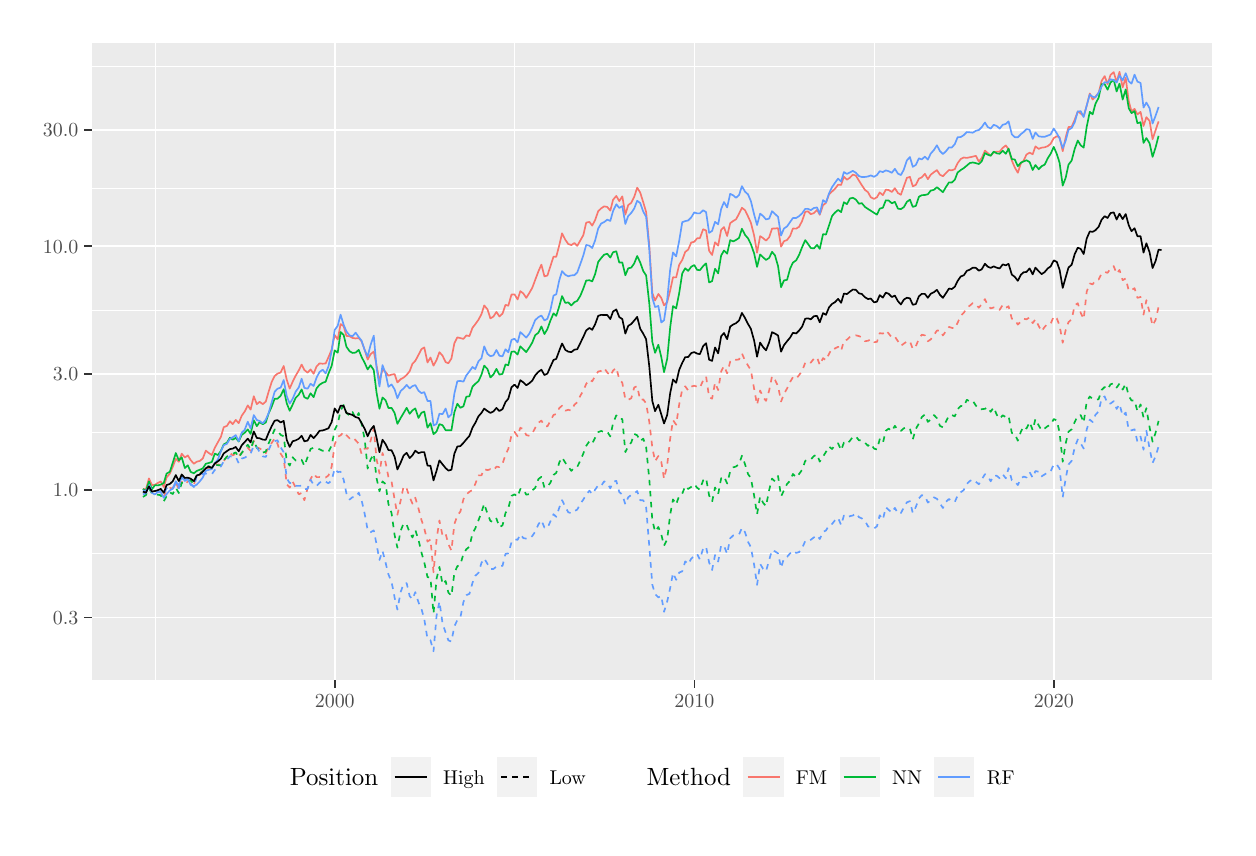
\begin{tikzpicture}[x=1pt,y=1pt]
\definecolor{fillColor}{RGB}{255,255,255}
\path[use as bounding box,fill=fillColor,fill opacity=0.00] (0,0) rectangle (433.62,289.08);
\begin{scope}
\path[clip] (  0.00,  0.00) rectangle (433.62,289.08);
\definecolor{drawColor}{RGB}{255,255,255}
\definecolor{fillColor}{RGB}{255,255,255}

\path[draw=drawColor,line width= 0.6pt,line join=round,line cap=round,fill=fillColor] (  0.00,  0.00) rectangle (433.62,289.08);
\end{scope}
\begin{scope}
\path[clip] ( 23.25, 53.26) rectangle (428.12,283.58);
\definecolor{fillColor}{gray}{0.92}

\path[fill=fillColor] ( 23.25, 53.26) rectangle (428.12,283.58);
\definecolor{drawColor}{RGB}{255,255,255}

\path[draw=drawColor,line width= 0.3pt,line join=round] ( 23.25, 98.94) --
	(428.12, 98.94);

\path[draw=drawColor,line width= 0.3pt,line join=round] ( 23.25,142.99) --
	(428.12,142.99);

\path[draw=drawColor,line width= 0.3pt,line join=round] ( 23.25,187.05) --
	(428.12,187.05);

\path[draw=drawColor,line width= 0.3pt,line join=round] ( 23.25,231.10) --
	(428.12,231.10);

\path[draw=drawColor,line width= 0.3pt,line join=round] ( 23.25,275.16) --
	(428.12,275.16);

\path[draw=drawColor,line width= 0.3pt,line join=round] ( 46.01, 53.26) --
	( 46.01,283.58);

\path[draw=drawColor,line width= 0.3pt,line join=round] (175.94, 53.26) --
	(175.94,283.58);

\path[draw=drawColor,line width= 0.3pt,line join=round] (305.86, 53.26) --
	(305.86,283.58);

\path[draw=drawColor,line width= 0.6pt,line join=round] ( 23.25, 75.90) --
	(428.12, 75.90);

\path[draw=drawColor,line width= 0.6pt,line join=round] ( 23.25,121.97) --
	(428.12,121.97);

\path[draw=drawColor,line width= 0.6pt,line join=round] ( 23.25,164.01) --
	(428.12,164.01);

\path[draw=drawColor,line width= 0.6pt,line join=round] ( 23.25,210.08) --
	(428.12,210.08);

\path[draw=drawColor,line width= 0.6pt,line join=round] ( 23.25,252.12) --
	(428.12,252.12);

\path[draw=drawColor,line width= 0.6pt,line join=round] (110.97, 53.26) --
	(110.97,283.58);

\path[draw=drawColor,line width= 0.6pt,line join=round] (240.91, 53.26) --
	(240.91,283.58);

\path[draw=drawColor,line width= 0.6pt,line join=round] (370.80, 53.26) --
	(370.80,283.58);
\definecolor{drawColor}{RGB}{248,118,109}

\path[draw=drawColor,line width= 0.6pt,line join=round] ( 41.65,122.42) --
	( 42.72,122.18) --
	( 43.82,126.20) --
	( 44.89,123.83) --
	( 45.95,123.88) --
	( 47.09,124.60) --
	( 48.09,125.11) --
	( 49.19,123.09) --
	( 50.19,126.54) --
	( 51.36,127.93) --
	( 52.43,130.39) --
	( 53.53,133.30) --
	( 54.63,132.20) --
	( 55.66,135.15) --
	( 56.80,133.77) --
	( 57.87,134.50) --
	( 58.90,132.81) --
	( 60.07,131.50) --
	( 61.11,132.26) --
	( 62.14,132.48) --
	( 63.28,133.40) --
	( 64.38,136.24) --
	( 65.37,135.43) --
	( 66.55,134.64) --
	( 67.62,137.26) --
	( 68.72,139.26) --
	( 69.82,141.21) --
	( 70.85,144.73) --
	( 71.99,145.17) --
	( 73.09,146.86) --
	( 74.09,145.81) --
	( 75.19,147.34) --
	( 76.26,146.17) --
	( 77.33,148.82) --
	( 78.43,150.39) --
	( 79.53,152.61) --
	( 80.56,151.05) --
	( 81.70,155.90) --
	( 82.80,153.02) --
	( 83.80,153.87) --
	( 84.97,153.05) --
	( 86.04,153.95) --
	( 87.04,157.44) --
	( 88.17,161.04) --
	( 89.24,163.20) --
	( 90.27,164.06) --
	( 91.41,164.49) --
	( 92.51,166.83) --
	( 93.62,161.81) --
	( 94.68,158.66) --
	( 95.75,161.12) --
	( 96.85,163.33) --
	( 97.96,165.24) --
	( 98.99,167.33) --
	( 99.98,165.38) --
	(101.16,164.42) --
	(102.22,165.60) --
	(103.33,164.03) --
	(104.39,166.68) --
	(105.46,167.77) --
	(106.60,167.65) --
	(107.67,167.75) --
	(108.70,170.00) --
	(109.84,172.77) --
	(110.94,178.03) --
	(112.04,176.41) --
	(113.07,181.99) --
	(114.18,181.22) --
	(115.17,177.69) --
	(116.34,177.58) --
	(117.41,176.96) --
	(118.51,176.78) --
	(119.62,176.94) --
	(120.65,175.74) --
	(121.79,172.61) --
	(122.85,169.14) --
	(123.89,171.07) --
	(125.06,172.05) --
	(126.06,167.04) --
	(127.12,161.38) --
	(128.22,165.61) --
	(129.33,164.66) --
	(130.36,163.32) --
	(131.50,163.72) --
	(132.60,163.89) --
	(133.60,160.89) --
	(134.77,162.05) --
	(135.84,162.63) --
	(136.94,163.59) --
	(138.04,164.97) --
	(139.04,167.62) --
	(140.07,168.69) --
	(141.21,170.82) --
	(142.31,172.93) --
	(143.31,173.54) --
	(144.48,168.08) --
	(145.55,169.88) --
	(146.65,166.96) --
	(147.75,168.98) --
	(148.78,171.82) --
	(149.92,170.54) --
	(151.02,168.24) --
	(152.02,167.81) --
	(153.12,169.53) --
	(154.19,175.06) --
	(155.26,177.16) --
	(156.36,176.91) --
	(157.46,176.61) --
	(158.49,177.86) --
	(159.63,177.64) --
	(160.73,180.63) --
	(161.73,181.91) --
	(162.90,183.54) --
	(163.97,185.54) --
	(164.97,188.71) --
	(166.14,187.31) --
	(167.21,184.01) --
	(168.31,184.70) --
	(169.38,186.37) --
	(170.45,184.73) --
	(171.58,185.74) --
	(172.65,188.92) --
	(173.68,188.61) --
	(174.82,192.64) --
	(175.92,192.72) --
	(177.03,190.87) --
	(178.02,193.87) --
	(179.12,193.02) --
	(180.16,191.43) --
	(181.29,193.25) --
	(182.36,195.13) --
	(183.39,197.93) --
	(184.57,201.05) --
	(185.63,203.46) --
	(186.74,199.19) --
	(187.80,199.52) --
	(188.87,202.83) --
	(190.01,206.35) --
	(191.00,206.31) --
	(192.11,210.53) --
	(193.10,214.77) --
	(194.28,212.43) --
	(195.34,210.90) --
	(196.45,210.52) --
	(197.55,211.26) --
	(198.58,210.23) --
	(199.72,212.23) --
	(200.79,214.13) --
	(201.82,218.63) --
	(202.99,218.89) --
	(203.99,217.56) --
	(205.05,219.58) --
	(206.16,222.78) --
	(207.26,223.80) --
	(208.29,224.51) --
	(209.43,224.29) --
	(210.53,222.95) --
	(211.53,226.90) --
	(212.70,228.27) --
	(213.77,226.41) --
	(214.87,228.13) --
	(215.97,221.54) --
	(217.00,224.95) --
	(218.11,225.81) --
	(219.17,227.92) --
	(220.24,231.26) --
	(221.34,229.49) --
	(222.45,225.94) --
	(223.48,222.45) --
	(224.62,210.36) --
	(225.72,193.17) --
	(226.71,190.50) --
	(227.89,192.85) --
	(228.96,191.41) --
	(229.95,188.73) --
	(231.09,189.89) --
	(232.16,194.09) --
	(233.19,198.88) --
	(234.33,198.83) --
	(235.43,203.41) --
	(236.53,205.16) --
	(237.60,208.04) --
	(238.67,208.88) --
	(239.77,211.44) --
	(240.87,211.71) --
	(241.90,212.97) --
	(242.90,213.02) --
	(244.07,216.23) --
	(245.14,215.82) --
	(246.24,208.44) --
	(247.31,206.95) --
	(248.38,211.55) --
	(249.51,210.31) --
	(250.58,216.05) --
	(251.61,217.03) --
	(252.75,213.80) --
	(253.85,218.43) --
	(254.96,219.25) --
	(255.95,219.81) --
	(257.06,221.85) --
	(258.09,223.99) --
	(259.22,223.12) --
	(260.29,220.89) --
	(261.32,218.63) --
	(262.50,213.98) --
	(263.56,207.76) --
	(264.67,213.74) --
	(265.73,213.04) --
	(266.80,212.13) --
	(267.94,213.34) --
	(268.97,216.47) --
	(270.04,216.52) --
	(271.14,216.62) --
	(272.24,209.94) --
	(273.27,211.91) --
	(274.41,212.36) --
	(275.52,213.84) --
	(276.51,216.50) --
	(277.69,216.45) --
	(278.75,217.13) --
	(279.85,219.25) --
	(280.96,222.54) --
	(281.95,222.72) --
	(282.98,221.69) --
	(284.12,222.07) --
	(285.23,223.23) --
	(286.22,221.48) --
	(287.40,224.91) --
	(288.46,225.78) --
	(289.57,228.87) --
	(290.67,229.89) --
	(291.70,230.83) --
	(292.84,232.33) --
	(293.94,232.25) --
	(294.94,235.24) --
	(296.04,234.13) --
	(297.11,234.87) --
	(298.17,236.00) --
	(299.28,235.60) --
	(300.38,233.80) --
	(301.41,232.16) --
	(302.55,230.46) --
	(303.65,229.62) --
	(304.65,227.78) --
	(305.82,227.20) --
	(306.89,227.81) --
	(307.88,229.52) --
	(309.02,228.57) --
	(310.09,230.53) --
	(311.12,230.40) --
	(312.26,229.70) --
	(313.36,231.06) --
	(314.46,229.32) --
	(315.53,228.70) --
	(316.60,231.74) --
	(317.70,234.81) --
	(318.80,235.17) --
	(319.83,231.76) --
	(320.94,232.27) --
	(322.04,234.51) --
	(323.07,234.99) --
	(324.21,236.28) --
	(325.28,234.33) --
	(326.31,235.95) --
	(327.48,236.86) --
	(328.55,237.61) --
	(329.65,235.91) --
	(330.72,235.41) --
	(331.79,236.51) --
	(332.92,237.65) --
	(333.92,237.51) --
	(335.02,237.97) --
	(336.02,240.11) --
	(337.19,241.65) --
	(338.26,242.16) --
	(339.36,242.01) --
	(340.46,242.26) --
	(341.50,242.47) --
	(342.63,242.77) --
	(343.70,240.70) --
	(344.73,241.95) --
	(345.91,244.65) --
	(346.90,243.79) --
	(347.97,242.84) --
	(349.07,244.02) --
	(350.17,244.29) --
	(351.21,244.27) --
	(352.34,245.66) --
	(353.45,246.51) --
	(354.44,245.17) --
	(355.62,241.09) --
	(356.68,238.58) --
	(357.79,236.65) --
	(358.89,240.07) --
	(359.88,241.02) --
	(360.92,243.24) --
	(362.05,243.91) --
	(363.16,243.34) --
	(364.15,246.18) --
	(365.33,245.29) --
	(366.39,245.72) --
	(367.50,245.85) --
	(368.60,246.28) --
	(369.63,247.11) --
	(370.77,249.18) --
	(371.87,249.84) --
	(372.87,249.47) --
	(374.01,244.46) --
	(375.07,249.38) --
	(376.10,253.16) --
	(377.24,253.28) --
	(378.34,255.81) --
	(379.45,258.81) --
	(380.51,258.06) --
	(381.58,257.15) --
	(382.68,260.91) --
	(383.79,265.30) --
	(384.82,263.12) --
	(385.81,264.16) --
	(386.99,265.48) --
	(388.06,269.83) --
	(389.16,271.58) --
	(390.22,268.68) --
	(391.29,272.02) --
	(392.43,273.00) --
	(393.50,269.42) --
	(394.53,273.11) --
	(395.67,267.51) --
	(396.77,270.95) --
	(397.87,262.50) --
	(398.87,258.84) --
	(399.97,259.73) --
	(401.00,257.73) --
	(402.14,258.64) --
	(403.21,253.57) --
	(404.24,256.73) --
	(405.41,255.37) --
	(406.48,248.77) --
	(407.58,252.09) --
	(408.65,255.20);

\path[draw=drawColor,line width= 0.6pt,dash pattern=on 2pt off 2pt ,line join=round] ( 41.65,122.41) --
	( 42.72,121.90) --
	( 43.82,124.38) --
	( 44.89,121.72) --
	( 45.95,121.67) --
	( 47.09,121.36) --
	( 48.09,121.10) --
	( 49.19,119.56) --
	( 50.19,122.23) --
	( 51.36,122.73) --
	( 52.43,122.66) --
	( 53.53,124.87) --
	( 54.63,122.10) --
	( 55.66,124.94) --
	( 56.80,123.97) --
	( 57.87,125.15) --
	( 58.90,125.60) --
	( 60.07,124.01) --
	( 61.11,127.28) --
	( 62.14,127.43) --
	( 63.28,129.61) --
	( 64.38,130.16) --
	( 65.37,129.91) --
	( 66.55,130.03) --
	( 67.62,131.66) --
	( 68.72,131.09) --
	( 69.82,131.63) --
	( 70.85,132.53) --
	( 71.99,133.98) --
	( 73.09,135.45) --
	( 74.09,134.48) --
	( 75.19,135.16) --
	( 76.26,134.23) --
	( 77.33,135.50) --
	( 78.43,136.02) --
	( 79.53,137.27) --
	( 80.56,136.14) --
	( 81.70,139.77) --
	( 82.80,137.38) --
	( 83.80,137.06) --
	( 84.97,136.32) --
	( 86.04,135.32) --
	( 87.04,137.62) --
	( 88.17,139.01) --
	( 89.24,140.65) --
	( 90.27,138.73) --
	( 91.41,135.15) --
	( 92.51,133.43) --
	( 93.62,124.06) --
	( 94.68,122.89) --
	( 95.75,125.10) --
	( 96.85,122.84) --
	( 97.96,120.46) --
	( 98.99,120.94) --
	( 99.98,118.33) --
	(101.16,122.68) --
	(102.22,125.97) --
	(103.33,127.92) --
	(104.39,126.66) --
	(105.46,126.69) --
	(106.60,126.36) --
	(107.67,126.53) --
	(108.70,127.27) --
	(109.84,130.44) --
	(110.94,138.47) --
	(112.04,141.25) --
	(113.07,141.76) --
	(114.18,142.99) --
	(115.17,141.83) --
	(116.34,140.65) --
	(117.41,141.12) --
	(118.51,140.00) --
	(119.62,138.75) --
	(120.65,135.03) --
	(121.79,137.02) --
	(122.85,136.92) --
	(123.89,139.71) --
	(125.06,144.23) --
	(126.06,133.23) --
	(127.12,127.99) --
	(128.22,135.40) --
	(129.33,131.92) --
	(130.36,126.64) --
	(131.50,125.02) --
	(132.60,118.51) --
	(133.60,113.07) --
	(134.77,118.18) --
	(135.84,123.37) --
	(136.94,122.51) --
	(138.04,119.44) --
	(139.04,117.08) --
	(140.07,119.23) --
	(141.21,115.34) --
	(142.31,111.12) --
	(143.31,108.14) --
	(144.48,103.38) --
	(145.55,104.13) --
	(146.65, 92.28) --
	(147.75,104.16) --
	(148.78,111.00) --
	(149.92,105.49) --
	(151.02,106.23) --
	(152.02,102.46) --
	(153.12,100.13) --
	(154.19,109.69) --
	(155.26,112.79) --
	(156.36,114.23) --
	(157.46,118.69) --
	(158.49,120.40) --
	(159.63,121.37) --
	(160.73,122.03) --
	(161.73,124.17) --
	(162.90,127.30) --
	(163.97,127.31) --
	(164.97,129.60) --
	(166.14,129.18) --
	(167.21,129.55) --
	(168.31,129.09) --
	(169.38,130.43) --
	(170.45,130.32) --
	(171.58,131.46) --
	(172.65,134.72) --
	(173.68,136.88) --
	(174.82,141.77) --
	(175.92,143.02) --
	(177.03,141.41) --
	(178.02,144.51) --
	(179.12,143.99) --
	(180.16,141.86) --
	(181.29,141.58) --
	(182.36,142.48) --
	(183.39,144.49) --
	(184.57,146.34) --
	(185.63,147.09) --
	(186.74,145.15) --
	(187.80,145.02) --
	(188.87,146.92) --
	(190.01,149.16) --
	(191.00,149.49) --
	(192.11,151.65) --
	(193.10,152.46) --
	(194.28,150.68) --
	(195.34,151.00) --
	(196.45,150.71) --
	(197.55,152.83) --
	(198.58,153.71) --
	(199.72,156.13) --
	(200.79,157.88) --
	(201.82,160.36) --
	(202.99,161.90) --
	(203.99,161.27) --
	(205.05,163.20) --
	(206.16,164.83) --
	(207.26,165.07) --
	(208.29,166.09) --
	(209.43,164.51) --
	(210.53,163.25) --
	(211.53,165.18) --
	(212.70,166.19) --
	(213.77,162.03) --
	(214.87,160.77) --
	(215.97,154.73) --
	(217.00,154.61) --
	(218.11,155.17) --
	(219.17,159.08) --
	(220.24,159.54) --
	(221.34,154.47) --
	(222.45,154.76) --
	(223.48,153.26) --
	(224.62,146.65) --
	(225.72,137.32) --
	(226.71,132.39) --
	(227.89,134.30) --
	(228.96,132.18) --
	(229.95,126.05) --
	(231.09,131.08) --
	(232.16,140.53) --
	(233.19,147.26) --
	(234.33,145.61) --
	(235.43,153.01) --
	(236.53,158.38) --
	(237.60,159.48) --
	(238.67,158.00) --
	(239.77,159.38) --
	(240.87,159.69) --
	(241.90,159.36) --
	(242.90,158.94) --
	(244.07,161.61) --
	(245.14,163.03) --
	(246.24,155.54) --
	(247.31,155.00) --
	(248.38,160.80) --
	(249.51,158.11) --
	(250.58,164.84) --
	(251.61,166.84) --
	(252.75,164.20) --
	(253.85,168.39) --
	(254.96,169.37) --
	(255.95,169.05) --
	(257.06,169.19) --
	(258.09,171.39) --
	(259.22,168.75) --
	(260.29,166.99) --
	(261.32,165.33) --
	(262.50,158.60) --
	(263.56,152.81) --
	(264.67,157.96) --
	(265.73,155.59) --
	(266.80,154.22) --
	(267.94,157.99) --
	(268.97,163.16) --
	(270.04,161.81) --
	(271.14,159.60) --
	(272.24,153.97) --
	(273.27,156.74) --
	(274.41,158.70) --
	(275.52,161.06) --
	(276.51,162.77) --
	(277.69,162.23) --
	(278.75,163.53) --
	(279.85,165.07) --
	(280.96,167.99) --
	(281.95,168.55) --
	(282.98,168.03) --
	(284.12,169.51) --
	(285.23,169.97) --
	(286.22,167.19) --
	(287.40,169.68) --
	(288.46,168.91) --
	(289.57,171.18) --
	(290.67,173.30) --
	(291.70,173.14) --
	(292.84,173.78) --
	(293.94,172.31) --
	(294.94,175.95) --
	(296.04,176.32) --
	(297.11,177.32) --
	(298.17,177.48) --
	(299.28,177.90) --
	(300.38,177.64) --
	(301.41,177.15) --
	(302.55,175.78) --
	(303.65,175.95) --
	(304.65,176.49) --
	(305.82,175.42) --
	(306.89,175.55) --
	(307.88,178.72) --
	(309.02,178.51) --
	(310.09,179.67) --
	(311.12,178.56) --
	(312.26,177.08) --
	(313.36,177.42) --
	(314.46,175.77) --
	(315.53,174.10) --
	(316.60,174.92) --
	(317.70,175.66) --
	(318.80,175.78) --
	(319.83,172.96) --
	(320.94,173.98) --
	(322.04,176.63) --
	(323.07,178.14) --
	(324.21,177.88) --
	(325.28,175.76) --
	(326.31,176.42) --
	(327.48,178.04) --
	(328.55,179.61) --
	(329.65,179.71) --
	(330.72,177.87) --
	(331.79,179.40) --
	(332.92,180.96) --
	(333.92,180.62) --
	(335.02,180.40) --
	(336.02,182.42) --
	(337.19,185.03) --
	(338.26,186.05) --
	(339.36,187.85) --
	(340.46,188.64) --
	(341.50,189.54) --
	(342.63,189.07) --
	(343.70,187.89) --
	(344.73,189.16) --
	(345.91,190.98) --
	(346.90,188.73) --
	(347.97,187.62) --
	(349.07,188.00) --
	(350.17,187.98) --
	(351.21,187.12) --
	(352.34,188.91) --
	(353.45,187.83) --
	(354.44,188.42) --
	(355.62,183.91) --
	(356.68,183.56) --
	(357.79,181.78) --
	(358.89,182.94) --
	(359.88,183.89) --
	(360.92,183.69) --
	(362.05,184.37) --
	(363.16,182.30) --
	(364.15,183.71) --
	(365.33,181.30) --
	(366.39,179.35) --
	(367.50,180.98) --
	(368.60,182.06) --
	(369.63,182.05) --
	(370.77,184.75) --
	(371.87,184.03) --
	(372.87,181.42) --
	(374.01,175.24) --
	(375.07,179.75) --
	(376.10,182.68) --
	(377.24,183.70) --
	(378.34,188.72) --
	(379.45,189.51) --
	(380.51,186.05) --
	(381.58,183.80) --
	(382.68,193.70) --
	(383.79,196.65) --
	(384.82,196.32) --
	(385.81,197.80) --
	(386.99,198.09) --
	(388.06,200.25) --
	(389.16,200.82) --
	(390.22,200.48) --
	(391.29,202.15) --
	(392.43,202.91) --
	(393.50,200.18) --
	(394.53,201.53) --
	(395.67,197.82) --
	(396.77,198.44) --
	(397.87,194.04) --
	(398.87,194.26) --
	(399.97,194.94) --
	(401.00,191.44) --
	(402.14,191.77) --
	(403.21,185.39) --
	(404.24,190.63) --
	(405.41,186.08) --
	(406.48,181.41) --
	(407.58,183.56) --
	(408.65,188.22);
\definecolor{drawColor}{RGB}{0,186,56}

\path[draw=drawColor,line width= 0.6pt,line join=round] ( 41.65,122.40) --
	( 42.72,121.63) --
	( 43.82,125.13) --
	( 44.89,122.27) --
	( 45.95,123.71) --
	( 47.09,123.70) --
	( 48.09,123.96) --
	( 49.19,124.56) --
	( 50.19,127.96) --
	( 51.36,128.57) --
	( 52.43,131.88) --
	( 53.53,135.37) --
	( 54.63,132.73) --
	( 55.66,133.83) --
	( 56.80,129.94) --
	( 57.87,130.93) --
	( 58.90,128.56) --
	( 60.07,128.05) --
	( 61.11,128.92) --
	( 62.14,129.31) --
	( 63.28,129.82) --
	( 64.38,131.51) --
	( 65.37,131.76) --
	( 66.55,132.13) --
	( 67.62,135.18) --
	( 68.72,134.62) --
	( 69.82,136.15) --
	( 70.85,138.49) --
	( 71.99,139.11) --
	( 73.09,140.92) --
	( 74.09,140.17) --
	( 75.19,140.88) --
	( 76.26,139.54) --
	( 77.33,141.90) --
	( 78.43,142.72) --
	( 79.53,143.90) --
	( 80.56,142.28) --
	( 81.70,147.25) --
	( 82.80,145.09) --
	( 83.80,146.55) --
	( 84.97,145.79) --
	( 86.04,146.42) --
	( 87.04,149.64) --
	( 88.17,152.13) --
	( 89.24,155.00) --
	( 90.27,155.01) --
	( 91.41,156.05) --
	( 92.51,158.43) --
	( 93.62,153.32) --
	( 94.68,150.65) --
	( 95.75,152.89) --
	( 96.85,155.36) --
	( 97.96,156.44) --
	( 98.99,158.36) --
	( 99.98,155.54) --
	(101.16,154.98) --
	(102.22,156.96) --
	(103.33,155.56) --
	(104.39,158.74) --
	(105.46,160.04) --
	(106.60,160.76) --
	(107.67,161.13) --
	(108.70,164.11) --
	(109.84,166.87) --
	(110.94,172.47) --
	(112.04,171.62) --
	(113.07,179.10) --
	(114.18,178.04) --
	(115.17,173.81) --
	(116.34,172.14) --
	(117.41,171.54) --
	(118.51,171.67) --
	(119.62,172.66) --
	(120.65,170.13) --
	(121.79,167.92) --
	(122.85,165.57) --
	(123.89,167.09) --
	(125.06,165.32) --
	(126.06,157.22) --
	(127.12,151.37) --
	(128.22,155.44) --
	(129.33,154.45) --
	(130.36,151.64) --
	(131.50,151.69) --
	(132.60,149.84) --
	(133.60,145.90) --
	(134.77,148.04) --
	(135.84,149.82) --
	(136.94,151.72) --
	(138.04,149.55) --
	(139.04,150.79) --
	(140.07,151.49) --
	(141.21,148.05) --
	(142.31,149.94) --
	(143.31,150.37) --
	(144.48,144.54) --
	(145.55,146.16) --
	(146.65,142.17) --
	(147.75,143.17) --
	(148.78,145.80) --
	(149.92,145.43) --
	(151.02,143.62) --
	(152.02,143.61) --
	(153.12,143.59) --
	(154.19,150.12) --
	(155.26,153.19) --
	(156.36,151.71) --
	(157.46,152.28) --
	(158.49,155.71) --
	(159.63,155.89) --
	(160.73,159.35) --
	(161.73,160.38) --
	(162.90,161.35) --
	(163.97,163.68) --
	(164.97,166.97) --
	(166.14,165.73) --
	(167.21,162.69) --
	(168.31,163.77) --
	(169.38,165.79) --
	(170.45,163.71) --
	(171.58,163.98) --
	(172.65,167.39) --
	(173.68,167.09) --
	(174.82,171.98) --
	(175.92,172.06) --
	(177.03,170.96) --
	(178.02,173.94) --
	(179.12,172.85) --
	(180.16,171.84) --
	(181.29,173.54) --
	(182.36,175.35) --
	(183.39,177.96) --
	(184.57,178.85) --
	(185.63,181.12) --
	(186.74,178.37) --
	(187.80,180.18) --
	(188.87,183.19) --
	(190.01,185.84) --
	(191.00,184.94) --
	(192.11,188.48) --
	(193.10,192.08) --
	(194.28,189.62) --
	(195.34,189.81) --
	(196.45,188.71) --
	(197.55,189.87) --
	(198.58,190.36) --
	(199.72,192.24) --
	(200.79,194.85) --
	(201.82,197.70) --
	(202.99,197.82) --
	(203.99,197.37) --
	(205.05,200.03) --
	(206.16,204.45) --
	(207.26,205.85) --
	(208.29,207.04) --
	(209.43,207.39) --
	(210.53,206.00) --
	(211.53,207.93) --
	(212.70,208.27) --
	(213.77,204.19) --
	(214.87,204.25) --
	(215.97,199.60) --
	(217.00,202.11) --
	(218.11,202.37) --
	(219.17,203.90) --
	(220.24,206.57) --
	(221.34,204.23) --
	(222.45,201.10) --
	(223.48,199.58) --
	(224.62,189.44) --
	(225.72,175.53) --
	(226.71,171.57) --
	(227.89,174.50) --
	(228.96,170.03) --
	(229.95,164.61) --
	(231.09,169.38) --
	(232.16,180.72) --
	(233.19,188.47) --
	(234.33,187.64) --
	(235.43,193.22) --
	(236.53,200.31) --
	(237.60,202.13) --
	(238.67,201.20) --
	(239.77,202.69) --
	(240.87,203.31) --
	(241.90,201.56) --
	(242.90,201.44) --
	(244.07,202.91) --
	(245.14,203.91) --
	(246.24,197.01) --
	(247.31,197.49) --
	(248.38,201.98) --
	(249.51,200.29) --
	(250.58,206.74) --
	(251.61,208.54) --
	(252.75,207.40) --
	(253.85,212.31) --
	(254.96,211.84) --
	(255.95,212.35) --
	(257.06,213.13) --
	(258.09,216.42) --
	(259.22,214.20) --
	(260.29,212.95) --
	(261.32,210.87) --
	(262.50,207.52) --
	(263.56,202.63) --
	(264.67,207.11) --
	(265.73,206.09) --
	(266.80,205.16) --
	(267.94,205.87) --
	(268.97,208.09) --
	(270.04,206.78) --
	(271.14,202.95) --
	(272.24,195.30) --
	(273.27,197.73) --
	(274.41,197.98) --
	(275.52,202.06) --
	(276.51,204.18) --
	(277.69,205.00) --
	(278.75,206.96) --
	(279.85,209.78) --
	(280.96,212.30) --
	(281.95,210.97) --
	(282.98,209.45) --
	(284.12,209.32) --
	(285.23,210.58) --
	(286.22,209.14) --
	(287.40,214.46) --
	(288.46,214.33) --
	(289.57,217.62) --
	(290.67,221.05) --
	(291.70,222.24) --
	(292.84,223.22) --
	(293.94,222.44) --
	(294.94,226.00) --
	(296.04,225.31) --
	(297.11,227.35) --
	(298.17,227.61) --
	(299.28,226.95) --
	(300.38,225.45) --
	(301.41,225.68) --
	(302.55,224.31) --
	(303.65,223.57) --
	(304.65,222.93) --
	(305.82,222.18) --
	(306.89,221.50) --
	(307.88,223.68) --
	(309.02,224.00) --
	(310.09,226.69) --
	(311.12,226.63) --
	(312.26,225.61) --
	(313.36,226.14) --
	(314.46,223.69) --
	(315.53,223.50) --
	(316.60,224.22) --
	(317.70,226.14) --
	(318.80,226.93) --
	(319.83,224.30) --
	(320.94,224.67) --
	(322.04,227.97) --
	(323.07,228.55) --
	(324.21,228.62) --
	(325.28,228.88) --
	(326.31,230.20) --
	(327.48,230.48) --
	(328.55,231.45) --
	(329.65,230.53) --
	(330.72,229.62) --
	(331.79,231.45) --
	(332.92,233.19) --
	(333.92,233.11) --
	(335.02,234.13) --
	(336.02,236.73) --
	(337.19,237.65) --
	(338.26,238.33) --
	(339.36,239.25) --
	(340.46,240.18) --
	(341.50,240.36) --
	(342.63,240.13) --
	(343.70,239.80) --
	(344.73,240.76) --
	(345.91,243.77) --
	(346.90,243.20) --
	(347.97,242.79) --
	(349.07,244.29) --
	(350.17,243.67) --
	(351.21,243.51) --
	(352.34,244.62) --
	(353.45,243.51) --
	(354.44,245.34) --
	(355.62,241.56) --
	(356.68,241.45) --
	(357.79,239.02) --
	(358.89,240.29) --
	(359.88,240.75) --
	(360.92,241.17) --
	(362.05,240.51) --
	(363.16,237.65) --
	(364.15,239.44) --
	(365.33,237.91) --
	(366.39,239.03) --
	(367.50,239.58) --
	(368.60,241.88) --
	(369.63,243.49) --
	(370.77,245.99) --
	(371.87,243.43) --
	(372.87,240.29) --
	(374.01,232.02) --
	(375.07,234.80) --
	(376.10,239.57) --
	(377.24,241.07) --
	(378.34,245.27) --
	(379.45,248.29) --
	(380.51,246.56) --
	(381.58,245.74) --
	(382.68,253.25) --
	(383.79,258.65) --
	(384.82,257.77) --
	(385.81,261.49) --
	(386.99,263.79) --
	(388.06,268.62) --
	(389.16,268.71) --
	(390.22,266.66) --
	(391.29,269.27) --
	(392.43,270.25) --
	(393.50,266.01) --
	(394.53,268.86) --
	(395.67,263.11) --
	(396.77,266.76) --
	(397.87,259.97) --
	(398.87,258.21) --
	(399.97,258.95) --
	(401.00,254.56) --
	(402.14,254.90) --
	(403.21,247.45) --
	(404.24,249.18) --
	(405.41,247.27) --
	(406.48,242.38) --
	(407.58,245.85) --
	(408.65,249.99);

\path[draw=drawColor,line width= 0.6pt,dash pattern=on 2pt off 2pt ,line join=round] ( 41.65,119.52) --
	( 42.72,120.16) --
	( 43.82,122.66) --
	( 44.89,120.78) --
	( 45.95,120.42) --
	( 47.09,120.31) --
	( 48.09,120.10) --
	( 49.19,117.89) --
	( 50.19,119.82) --
	( 51.36,121.17) --
	( 52.43,120.57) --
	( 53.53,122.79) --
	( 54.63,120.91) --
	( 55.66,124.61) --
	( 56.80,124.73) --
	( 57.87,125.20) --
	( 58.90,125.47) --
	( 60.07,124.07) --
	( 61.11,127.99) --
	( 62.14,127.83) --
	( 63.28,128.79) --
	( 64.38,130.36) --
	( 65.37,130.66) --
	( 66.55,129.83) --
	( 67.62,131.13) --
	( 68.72,130.99) --
	( 69.82,130.89) --
	( 70.85,132.70) --
	( 71.99,134.11) --
	( 73.09,134.59) --
	( 74.09,135.07) --
	( 75.19,135.60) --
	( 76.26,133.81) --
	( 77.33,135.35) --
	( 78.43,137.12) --
	( 79.53,138.34) --
	( 80.56,136.74) --
	( 81.70,140.04) --
	( 82.80,137.22) --
	( 83.80,136.69) --
	( 84.97,135.55) --
	( 86.04,135.87) --
	( 87.04,138.77) --
	( 88.17,141.37) --
	( 89.24,143.87) --
	( 90.27,143.66) --
	( 91.41,141.93) --
	( 92.51,141.41) --
	( 93.62,132.50) --
	( 94.68,130.81) --
	( 95.75,133.83) --
	( 96.85,132.68) --
	( 97.96,132.51) --
	( 98.99,132.95) --
	( 99.98,130.73) --
	(101.16,133.91) --
	(102.22,136.85) --
	(103.33,137.29) --
	(104.39,137.12) --
	(105.46,136.73) --
	(106.60,136.19) --
	(107.67,136.29) --
	(108.70,135.84) --
	(109.84,138.05) --
	(110.94,143.77) --
	(112.04,145.88) --
	(113.07,150.72) --
	(114.18,152.71) --
	(115.17,149.86) --
	(116.34,148.86) --
	(117.41,150.19) --
	(118.51,147.80) --
	(119.62,149.85) --
	(120.65,145.97) --
	(121.79,140.26) --
	(122.85,129.76) --
	(123.89,132.97) --
	(125.06,135.08) --
	(126.06,126.35) --
	(127.12,121.55) --
	(128.22,125.12) --
	(129.33,124.17) --
	(130.36,116.89) --
	(131.50,113.60) --
	(132.60,105.68) --
	(133.60,101.17) --
	(134.77,107.25) --
	(135.84,109.96) --
	(136.94,109.49) --
	(138.04,106.68) --
	(139.04,104.87) --
	(140.07,107.56) --
	(141.21,104.07) --
	(142.31, 99.36) --
	(143.31, 95.85) --
	(144.48, 90.53) --
	(145.55, 90.34) --
	(146.65, 77.35) --
	(147.75, 89.90) --
	(148.78, 94.25) --
	(149.92, 87.94) --
	(151.02, 89.14) --
	(152.02, 84.94) --
	(153.12, 83.81) --
	(154.19, 92.07) --
	(155.26, 94.48) --
	(156.36, 95.10) --
	(157.46, 98.93) --
	(158.49,100.60) --
	(159.63,101.54) --
	(160.73,106.32) --
	(161.73,108.12) --
	(162.90,111.07) --
	(163.97,113.95) --
	(164.97,117.09) --
	(166.14,113.43) --
	(167.21,110.84) --
	(168.31,110.38) --
	(169.38,111.72) --
	(170.45,108.61) --
	(171.58,109.23) --
	(172.65,113.67) --
	(173.68,115.42) --
	(174.82,119.89) --
	(175.92,120.46) --
	(177.03,119.57) --
	(178.02,122.38) --
	(179.12,122.31) --
	(180.16,120.32) --
	(181.29,120.54) --
	(182.36,121.90) --
	(183.39,122.77) --
	(184.57,125.98) --
	(185.63,126.76) --
	(186.74,122.83) --
	(187.80,123.19) --
	(188.87,124.64) --
	(190.01,127.46) --
	(191.00,128.21) --
	(192.11,132.02) --
	(193.10,133.78) --
	(194.28,131.86) --
	(195.34,130.49) --
	(196.45,128.93) --
	(197.55,130.17) --
	(198.58,130.35) --
	(199.72,132.67) --
	(200.79,135.23) --
	(201.82,137.94) --
	(202.99,139.68) --
	(203.99,138.84) --
	(205.05,140.91) --
	(206.16,142.94) --
	(207.26,143.35) --
	(208.29,142.88) --
	(209.43,143.09) --
	(210.53,141.37) --
	(211.53,146.22) --
	(212.70,148.99) --
	(213.77,147.59) --
	(214.87,147.69) --
	(215.97,135.70) --
	(217.00,137.78) --
	(218.11,139.21) --
	(219.17,142.31) --
	(220.24,141.79) --
	(221.34,139.71) --
	(222.45,140.57) --
	(223.48,137.51) --
	(224.62,125.87) --
	(225.72,111.08) --
	(226.71,106.99) --
	(227.89,108.65) --
	(228.96,105.95) --
	(229.95,101.89) --
	(231.09,104.18) --
	(232.16,113.07) --
	(233.19,118.62) --
	(234.33,116.79) --
	(235.43,119.99) --
	(236.53,120.67) --
	(237.60,123.46) --
	(238.67,122.40) --
	(239.77,123.14) --
	(240.87,124.14) --
	(241.90,122.81) --
	(242.90,122.12) --
	(244.07,125.50) --
	(245.14,126.30) --
	(246.24,120.02) --
	(247.31,117.75) --
	(248.38,122.92) --
	(249.51,120.52) --
	(250.58,126.25) --
	(251.61,126.95) --
	(252.75,124.38) --
	(253.85,128.74) --
	(254.96,130.20) --
	(255.95,130.51) --
	(257.06,131.40) --
	(258.09,134.41) --
	(259.22,131.31) --
	(260.29,127.81) --
	(261.32,126.32) --
	(262.50,119.99) --
	(263.56,113.21) --
	(264.67,119.62) --
	(265.73,117.40) --
	(266.80,116.18) --
	(267.94,122.00) --
	(268.97,126.13) --
	(270.04,125.15) --
	(271.14,127.08) --
	(272.24,119.72) --
	(273.27,121.86) --
	(274.41,124.22) --
	(275.52,125.40) --
	(276.51,127.82) --
	(277.69,126.56) --
	(278.75,127.79) --
	(279.85,129.33) --
	(280.96,132.52) --
	(281.95,133.01) --
	(282.98,133.04) --
	(284.12,134.31) --
	(285.23,134.86) --
	(286.22,132.28) --
	(287.40,134.10) --
	(288.46,135.78) --
	(289.57,137.69) --
	(290.67,136.83) --
	(291.70,138.26) --
	(292.84,138.89) --
	(293.94,136.37) --
	(294.94,139.15) --
	(296.04,138.69) --
	(297.11,139.81) --
	(298.17,141.19) --
	(299.28,141.39) --
	(300.38,139.95) --
	(301.41,140.00) --
	(302.55,139.13) --
	(303.65,137.95) --
	(304.65,138.78) --
	(305.82,136.96) --
	(306.89,136.68) --
	(307.88,140.34) --
	(309.02,139.01) --
	(310.09,143.43) --
	(311.12,144.19) --
	(312.26,143.27) --
	(313.36,145.22) --
	(314.46,143.60) --
	(315.53,143.37) --
	(316.60,144.31) --
	(317.70,144.62) --
	(318.80,144.23) --
	(319.83,140.31) --
	(320.94,144.12) --
	(322.04,146.02) --
	(323.07,148.34) --
	(324.21,149.30) --
	(325.28,146.64) --
	(326.31,147.46) --
	(327.48,149.08) --
	(328.55,147.99) --
	(329.65,145.19) --
	(330.72,144.65) --
	(331.79,146.70) --
	(332.92,148.96) --
	(333.92,149.08) --
	(335.02,148.64) --
	(336.02,151.23) --
	(337.19,152.38) --
	(338.26,152.21) --
	(339.36,154.60) --
	(340.46,154.02) --
	(341.50,154.25) --
	(342.63,152.52) --
	(343.70,151.20) --
	(344.73,151.21) --
	(345.91,151.35) --
	(346.90,151.95) --
	(347.97,150.27) --
	(349.07,151.90) --
	(350.17,149.20) --
	(351.21,147.77) --
	(352.34,149.00) --
	(353.45,148.36) --
	(354.44,148.79) --
	(355.62,142.60) --
	(356.68,142.37) --
	(357.79,139.83) --
	(358.89,143.09) --
	(359.88,145.01) --
	(360.92,144.24) --
	(362.05,146.55) --
	(363.16,143.68) --
	(364.15,147.65) --
	(365.33,145.35) --
	(366.39,143.57) --
	(367.50,144.27) --
	(368.60,145.12) --
	(369.63,145.53) --
	(370.77,147.66) --
	(371.87,147.15) --
	(372.87,142.79) --
	(374.01,132.22) --
	(375.07,138.82) --
	(376.10,143.08) --
	(377.24,143.96) --
	(378.34,146.57) --
	(379.45,148.88) --
	(380.51,149.09) --
	(381.58,146.39) --
	(382.68,153.93) --
	(383.79,155.80) --
	(384.82,154.88) --
	(385.81,154.62) --
	(386.99,154.83) --
	(388.06,158.17) --
	(389.16,159.23) --
	(390.22,158.37) --
	(391.29,160.22) --
	(392.43,160.59) --
	(393.50,159.03) --
	(394.53,160.47) --
	(395.67,158.31) --
	(396.77,160.41) --
	(397.87,155.99) --
	(398.87,154.34) --
	(399.97,154.39) --
	(401.00,150.45) --
	(402.14,152.95) --
	(403.21,148.22) --
	(404.24,151.58) --
	(405.41,144.60) --
	(406.48,139.48) --
	(407.58,142.78) --
	(408.65,146.98);
\definecolor{drawColor}{RGB}{97,156,255}

\path[draw=drawColor,line width= 0.6pt,line join=round] ( 41.65,120.42) --
	( 42.72,120.87) --
	( 43.82,123.34) --
	( 44.89,120.99) --
	( 45.95,120.41) --
	( 47.09,121.38) --
	( 48.09,121.26) --
	( 49.19,119.19) --
	( 50.19,120.51) --
	( 51.36,121.88) --
	( 52.43,122.50) --
	( 53.53,125.16) --
	( 54.63,123.42) --
	( 55.66,127.08) --
	( 56.80,125.27) --
	( 57.87,126.11) --
	( 58.90,123.85) --
	( 60.07,123.39) --
	( 61.11,123.98) --
	( 62.14,125.08) --
	( 63.28,126.51) --
	( 64.38,129.00) --
	( 65.37,129.29) --
	( 66.55,129.58) --
	( 67.62,131.71) --
	( 68.72,133.00) --
	( 69.82,135.98) --
	( 70.85,138.21) --
	( 71.99,138.69) --
	( 73.09,140.50) --
	( 74.09,141.09) --
	( 75.19,141.84) --
	( 76.26,139.65) --
	( 77.33,142.75) --
	( 78.43,143.77) --
	( 79.53,146.68) --
	( 80.56,144.25) --
	( 81.70,149.10) --
	( 82.80,147.30) --
	( 83.80,146.98) --
	( 84.97,146.09) --
	( 86.04,147.45) --
	( 87.04,149.72) --
	( 88.17,153.70) --
	( 89.24,157.51) --
	( 90.27,158.61) --
	( 91.41,159.01) --
	( 92.51,161.75) --
	( 93.62,155.93) --
	( 94.68,153.26) --
	( 95.75,154.96) --
	( 96.85,157.59) --
	( 97.96,159.08) --
	( 98.99,162.22) --
	( 99.98,158.92) --
	(101.16,158.63) --
	(102.22,160.41) --
	(103.33,159.60) --
	(104.39,162.64) --
	(105.46,164.67) --
	(106.60,165.47) --
	(107.67,164.17) --
	(108.70,166.68) --
	(109.84,172.24) --
	(110.94,179.85) --
	(112.04,181.36) --
	(113.07,185.38) --
	(114.18,181.71) --
	(115.17,179.32) --
	(116.34,177.86) --
	(117.41,177.61) --
	(118.51,178.86) --
	(119.62,177.28) --
	(120.65,176.00) --
	(121.79,172.55) --
	(122.85,170.26) --
	(123.89,174.38) --
	(125.06,177.80) --
	(126.06,166.24) --
	(127.12,159.42) --
	(128.22,167.15) --
	(129.33,164.13) --
	(130.36,159.31) --
	(131.50,160.15) --
	(132.60,158.36) --
	(133.60,155.15) --
	(134.77,157.78) --
	(135.84,158.72) --
	(136.94,159.99) --
	(138.04,158.71) --
	(139.04,159.54) --
	(140.07,159.94) --
	(141.21,157.89) --
	(142.31,157.03) --
	(143.31,157.38) --
	(144.48,154.17) --
	(145.55,154.20) --
	(146.65,145.34) --
	(147.75,145.86) --
	(148.78,149.59) --
	(149.92,149.42) --
	(151.02,151.44) --
	(152.02,148.26) --
	(153.12,149.33) --
	(154.19,156.89) --
	(155.26,161.32) --
	(156.36,161.44) --
	(157.46,161.16) --
	(158.49,163.40) --
	(159.63,164.88) --
	(160.73,166.46) --
	(161.73,165.73) --
	(162.90,168.54) --
	(163.97,169.60) --
	(164.97,173.92) --
	(166.14,171.19) --
	(167.21,170.36) --
	(168.31,170.66) --
	(169.38,172.61) --
	(170.45,170.55) --
	(171.58,170.30) --
	(172.65,172.87) --
	(173.68,171.76) --
	(174.82,176.27) --
	(175.92,176.67) --
	(177.03,175.36) --
	(178.02,179.08) --
	(179.12,178.06) --
	(180.16,177.08) --
	(181.29,178.53) --
	(182.36,180.84) --
	(183.39,183.41) --
	(184.57,184.49) --
	(185.63,185.07) --
	(186.74,183.27) --
	(187.80,183.88) --
	(188.87,186.94) --
	(190.01,192.28) --
	(191.00,192.75) --
	(192.11,197.89) --
	(193.10,201.09) --
	(194.28,199.78) --
	(195.34,199.24) --
	(196.45,199.57) --
	(197.55,199.64) --
	(198.58,200.62) --
	(199.72,203.73) --
	(200.79,206.81) --
	(201.82,210.56) --
	(202.99,210.28) --
	(203.99,209.46) --
	(205.05,212.20) --
	(206.16,216.52) --
	(207.26,218.34) --
	(208.29,218.81) --
	(209.43,219.70) --
	(210.53,219.24) --
	(211.53,222.83) --
	(212.70,225.26) --
	(213.77,223.94) --
	(214.87,224.61) --
	(215.97,218.15) --
	(217.00,221.03) --
	(218.11,222.15) --
	(219.17,223.72) --
	(220.24,226.53) --
	(221.34,225.72) --
	(222.45,222.58) --
	(223.48,220.74) --
	(224.62,209.03) --
	(225.72,191.45) --
	(226.71,188.14) --
	(227.89,188.52) --
	(228.96,182.55) --
	(229.95,183.35) --
	(231.09,190.75) --
	(232.16,201.65) --
	(233.19,207.85) --
	(234.33,206.43) --
	(235.43,212.09) --
	(236.53,218.81) --
	(237.60,219.17) --
	(238.67,219.42) --
	(239.77,220.52) --
	(240.87,222.33) --
	(241.90,221.96) --
	(242.90,221.97) --
	(244.07,223.10) --
	(245.14,222.43) --
	(246.24,214.94) --
	(247.31,215.65) --
	(248.38,218.90) --
	(249.51,218.03) --
	(250.58,223.54) --
	(251.61,226.06) --
	(252.75,224.12) --
	(253.85,229.06) --
	(254.96,228.47) --
	(255.95,227.60) --
	(257.06,228.60) --
	(258.09,231.81) --
	(259.22,229.80) --
	(260.29,228.85) --
	(261.32,226.45) --
	(262.50,221.59) --
	(263.56,217.76) --
	(264.67,221.87) --
	(265.73,221.03) --
	(266.80,219.78) --
	(267.94,220.09) --
	(268.97,222.75) --
	(270.04,221.76) --
	(271.14,220.76) --
	(272.24,213.97) --
	(273.27,216.50) --
	(274.41,217.27) --
	(275.52,218.87) --
	(276.51,220.30) --
	(277.69,220.31) --
	(278.75,220.98) --
	(279.85,221.99) --
	(280.96,223.59) --
	(281.95,223.62) --
	(282.98,223.14) --
	(284.12,223.92) --
	(285.23,224.12) --
	(286.22,221.76) --
	(287.40,226.76) --
	(288.46,225.92) --
	(289.57,229.22) --
	(290.67,231.47) --
	(291.70,232.98) --
	(292.84,234.54) --
	(293.94,233.46) --
	(294.94,236.91) --
	(296.04,236.22) --
	(297.11,236.77) --
	(298.17,237.34) --
	(299.28,236.63) --
	(300.38,235.44) --
	(301.41,235.10) --
	(302.55,235.14) --
	(303.65,235.31) --
	(304.65,235.69) --
	(305.82,235.19) --
	(306.89,235.83) --
	(307.88,237.22) --
	(309.02,236.90) --
	(310.09,237.52) --
	(311.12,237.20) --
	(312.26,236.64) --
	(313.36,238.07) --
	(314.46,236.36) --
	(315.53,235.81) --
	(316.60,237.80) --
	(317.70,241.10) --
	(318.80,242.35) --
	(319.83,238.80) --
	(320.94,239.47) --
	(322.04,241.88) --
	(323.07,241.45) --
	(324.21,242.49) --
	(325.28,241.39) --
	(326.31,243.57) --
	(327.48,244.89) --
	(328.55,246.58) --
	(329.65,244.47) --
	(330.72,243.41) --
	(331.79,244.39) --
	(332.92,245.83) --
	(333.92,245.76) --
	(335.02,246.99) --
	(336.02,249.47) --
	(337.19,249.57) --
	(338.26,250.26) --
	(339.36,251.35) --
	(340.46,251.26) --
	(341.50,251.12) --
	(342.63,251.82) --
	(343.70,252.10) --
	(344.73,253.10) --
	(345.91,254.82) --
	(346.90,253.18) --
	(347.97,252.63) --
	(349.07,253.97) --
	(350.17,253.56) --
	(351.21,252.60) --
	(352.34,253.99) --
	(353.45,254.31) --
	(354.44,255.21) --
	(355.62,250.55) --
	(356.68,249.51) --
	(357.79,249.46) --
	(358.89,250.59) --
	(359.88,251.37) --
	(360.92,252.42) --
	(362.05,252.17) --
	(363.16,248.89) --
	(364.15,251.19) --
	(365.33,249.82) --
	(366.39,249.66) --
	(367.50,249.65) --
	(368.60,250.07) --
	(369.63,250.47) --
	(370.77,252.64) --
	(371.87,250.92) --
	(372.87,249.08) --
	(374.01,245.58) --
	(375.07,248.19) --
	(376.10,252.18) --
	(377.24,252.81) --
	(378.34,254.88) --
	(379.45,258.78) --
	(380.51,258.89) --
	(381.58,256.78) --
	(382.68,260.94) --
	(383.79,264.93) --
	(384.82,264.11) --
	(385.81,263.85) --
	(386.99,265.61) --
	(388.06,267.85) --
	(389.16,269.38) --
	(390.22,269.20) --
	(391.29,270.44) --
	(392.43,270.13) --
	(393.50,269.27) --
	(394.53,271.82) --
	(395.67,270.02) --
	(396.77,272.62) --
	(397.87,269.69) --
	(398.87,268.84) --
	(399.97,272.10) --
	(401.00,269.58) --
	(402.14,269.11) --
	(403.21,260.22) --
	(404.24,262.01) --
	(405.41,259.94) --
	(406.48,254.46) --
	(407.58,257.27) --
	(408.65,260.42);

\path[draw=drawColor,line width= 0.6pt,dash pattern=on 2pt off 2pt ,line join=round] ( 41.65,121.87) --
	( 42.72,121.59) --
	( 43.82,124.14) --
	( 44.89,121.64) --
	( 45.95,121.62) --
	( 47.09,121.34) --
	( 48.09,121.60) --
	( 49.19,120.56) --
	( 50.19,122.57) --
	( 51.36,122.95) --
	( 52.43,122.43) --
	( 53.53,124.49) --
	( 54.63,122.56) --
	( 55.66,126.23) --
	( 56.80,125.91) --
	( 57.87,124.89) --
	( 58.90,124.29) --
	( 60.07,123.06) --
	( 61.11,127.16) --
	( 62.14,127.60) --
	( 63.28,127.81) --
	( 64.38,127.93) --
	( 65.37,127.91) --
	( 66.55,127.67) --
	( 67.62,129.29) --
	( 68.72,129.66) --
	( 69.82,130.52) --
	( 70.85,132.38) --
	( 71.99,132.93) --
	( 73.09,134.23) --
	( 74.09,134.05) --
	( 75.19,134.01) --
	( 76.26,131.65) --
	( 77.33,133.35) --
	( 78.43,133.71) --
	( 79.53,134.34) --
	( 80.56,135.13) --
	( 81.70,138.10) --
	( 82.80,137.40) --
	( 83.80,135.79) --
	( 84.97,134.17) --
	( 86.04,133.96) --
	( 87.04,136.37) --
	( 88.17,138.96) --
	( 89.24,139.66) --
	( 90.27,139.99) --
	( 91.41,137.46) --
	( 92.51,135.68) --
	( 93.62,126.20) --
	( 94.68,124.55) --
	( 95.75,124.54) --
	( 96.85,123.53) --
	( 97.96,123.50) --
	( 98.99,123.55) --
	( 99.98,122.28) --
	(101.16,122.44) --
	(102.22,125.77) --
	(103.33,123.83) --
	(104.39,123.46) --
	(105.46,124.61) --
	(106.60,125.40) --
	(107.67,125.01) --
	(108.70,124.44) --
	(109.84,125.53) --
	(110.94,129.71) --
	(112.04,128.51) --
	(113.07,128.62) --
	(114.18,125.72) --
	(115.17,120.82) --
	(116.34,118.59) --
	(117.41,119.45) --
	(118.51,119.36) --
	(119.62,121.05) --
	(120.65,118.39) --
	(121.79,113.32) --
	(122.85,107.56) --
	(123.89,106.73) --
	(125.06,107.44) --
	(126.06,102.43) --
	(127.12, 96.75) --
	(128.22,100.02) --
	(129.33, 95.75) --
	(130.36, 91.52) --
	(131.50, 88.81) --
	(132.60, 83.08) --
	(133.60, 78.82) --
	(134.77, 85.12) --
	(135.84, 88.13) --
	(136.94, 88.37) --
	(138.04, 83.65) --
	(139.04, 82.57) --
	(140.07, 85.11) --
	(141.21, 81.46) --
	(142.31, 78.99) --
	(143.31, 75.33) --
	(144.48, 68.12) --
	(145.55, 67.70) --
	(146.65, 63.73) --
	(147.75, 76.57) --
	(148.78, 81.73) --
	(149.92, 73.76) --
	(151.02, 70.54) --
	(152.02, 67.67) --
	(153.12, 67.29) --
	(154.19, 72.82) --
	(155.26, 74.98) --
	(156.36, 75.96) --
	(157.46, 81.53) --
	(158.49, 84.02) --
	(159.63, 84.50) --
	(160.73, 88.45) --
	(161.73, 91.00) --
	(162.90, 92.09) --
	(163.97, 95.66) --
	(164.97, 97.31) --
	(166.14, 95.32) --
	(167.21, 93.50) --
	(168.31, 93.49) --
	(169.38, 94.36) --
	(170.45, 94.39) --
	(171.58, 94.62) --
	(172.65, 98.92) --
	(173.68, 99.15) --
	(174.82,103.07) --
	(175.92,104.28) --
	(177.03,103.99) --
	(178.02,106.01) --
	(179.12,104.64) --
	(180.16,104.44) --
	(181.29,104.46) --
	(182.36,105.43) --
	(183.39,106.95) --
	(184.57,109.63) --
	(185.63,111.10) --
	(186.74,108.44) --
	(187.80,108.21) --
	(188.87,110.63) --
	(190.01,113.26) --
	(191.00,112.33) --
	(192.11,115.68) --
	(193.10,118.34) --
	(194.28,115.93) --
	(195.34,113.96) --
	(196.45,113.59) --
	(197.55,114.40) --
	(198.58,114.94) --
	(199.72,117.03) --
	(200.79,118.58) --
	(201.82,120.35) --
	(202.99,121.76) --
	(203.99,120.52) --
	(205.05,122.14) --
	(206.16,123.74) --
	(207.26,123.51) --
	(208.29,125.16) --
	(209.43,124.45) --
	(210.53,122.64) --
	(211.53,124.94) --
	(212.70,125.33) --
	(213.77,121.27) --
	(214.87,120.37) --
	(215.97,116.81) --
	(217.00,119.38) --
	(218.11,120.24) --
	(219.17,120.74) --
	(220.24,121.64) --
	(221.34,118.33) --
	(222.45,118.28) --
	(223.48,115.78) --
	(224.62,101.64) --
	(225.72, 87.77) --
	(226.71, 84.42) --
	(227.89, 83.21) --
	(228.96, 83.76) --
	(229.95, 78.00) --
	(231.09, 81.76) --
	(232.16, 86.55) --
	(233.19, 92.02) --
	(234.33, 89.56) --
	(235.43, 92.20) --
	(236.53, 92.61) --
	(237.60, 96.22) --
	(238.67, 95.21) --
	(239.77, 97.19) --
	(240.87, 98.20) --
	(241.90, 98.92) --
	(242.90, 96.93) --
	(244.07,100.90) --
	(245.14,101.54) --
	(246.24, 95.82) --
	(247.31, 93.10) --
	(248.38, 98.50) --
	(249.51, 96.15) --
	(250.58,102.02) --
	(251.61,101.89) --
	(252.75, 98.94) --
	(253.85,104.55) --
	(254.96,105.61) --
	(255.95,105.63) --
	(257.06,105.93) --
	(258.09,108.35) --
	(259.22,106.75) --
	(260.29,103.32) --
	(261.32,101.36) --
	(262.50, 95.02) --
	(263.56, 87.72) --
	(264.67, 95.34) --
	(265.73, 93.55) --
	(266.80, 92.63) --
	(267.94, 96.77) --
	(268.97,100.31) --
	(270.04, 99.83) --
	(271.14, 99.11) --
	(272.24, 93.87) --
	(273.27, 97.32) --
	(274.41, 97.88) --
	(275.52, 99.14) --
	(276.51,100.03) --
	(277.69, 99.29) --
	(278.75, 99.57) --
	(279.85,101.03) --
	(280.96,103.54) --
	(281.95,103.42) --
	(282.98,104.03) --
	(284.12,104.90) --
	(285.23,105.67) --
	(286.22,104.28) --
	(287.40,106.93) --
	(288.46,107.36) --
	(289.57,109.35) --
	(290.67,109.74) --
	(291.70,111.05) --
	(292.84,111.98) --
	(293.94,109.33) --
	(294.94,112.79) --
	(296.04,112.07) --
	(297.11,112.56) --
	(298.17,112.81) --
	(299.28,113.60) --
	(300.38,112.21) --
	(301.41,111.75) --
	(302.55,110.94) --
	(303.65,108.82) --
	(304.65,108.75) --
	(305.82,108.10) --
	(306.89,108.92) --
	(307.88,112.88) --
	(309.02,111.31) --
	(310.09,115.76) --
	(311.12,114.84) --
	(312.26,113.84) --
	(313.36,115.56) --
	(314.46,113.47) --
	(315.53,113.68) --
	(316.60,115.67) --
	(317.70,117.57) --
	(318.80,117.97) --
	(319.83,113.67) --
	(320.94,115.91) --
	(322.04,118.95) --
	(323.07,120.16) --
	(324.21,119.86) --
	(325.28,117.47) --
	(326.31,118.28) --
	(327.48,119.36) --
	(328.55,118.84) --
	(329.65,117.21) --
	(330.72,115.50) --
	(331.79,117.72) --
	(332.92,118.79) --
	(333.92,117.85) --
	(335.02,117.71) --
	(336.02,119.99) --
	(337.19,121.22) --
	(338.26,122.01) --
	(339.36,124.23) --
	(340.46,125.27) --
	(341.50,125.83) --
	(342.63,124.97) --
	(343.70,124.10) --
	(344.73,125.80) --
	(345.91,127.74) --
	(346.90,127.16) --
	(347.97,125.16) --
	(349.07,127.27) --
	(350.17,127.16) --
	(351.21,126.27) --
	(352.34,127.71) --
	(353.45,126.24) --
	(354.44,129.92) --
	(355.62,125.57) --
	(356.68,125.25) --
	(357.79,123.80) --
	(358.89,126.14) --
	(359.88,126.87) --
	(360.92,126.54) --
	(362.05,128.45) --
	(363.16,126.46) --
	(364.15,128.87) --
	(365.33,128.61) --
	(366.39,126.94) --
	(367.50,127.66) --
	(368.60,128.38) --
	(369.63,128.65) --
	(370.77,131.35) --
	(371.87,131.20) --
	(372.87,129.76) --
	(374.01,119.39) --
	(375.07,126.14) --
	(376.10,131.24) --
	(377.24,132.54) --
	(378.34,137.35) --
	(379.45,140.27) --
	(380.51,138.87) --
	(381.58,136.99) --
	(382.68,143.91) --
	(383.79,147.45) --
	(384.82,146.56) --
	(385.81,149.15) --
	(386.99,150.40) --
	(388.06,155.13) --
	(389.16,155.83) --
	(390.22,153.15) --
	(391.29,153.26) --
	(392.43,154.11) --
	(393.50,151.31) --
	(394.53,153.07) --
	(395.67,148.81) --
	(396.77,149.97) --
	(397.87,143.61) --
	(398.87,143.57) --
	(399.97,143.96) --
	(401.00,139.47) --
	(402.14,141.33) --
	(403.21,136.58) --
	(404.24,143.43) --
	(405.41,136.91) --
	(406.48,131.79) --
	(407.58,134.21) --
	(408.65,137.80);
\definecolor{drawColor}{RGB}{0,0,0}

\path[draw=drawColor,line width= 0.6pt,line join=round] ( 41.65,121.44) --
	( 42.72,121.05) --
	( 43.82,123.32) --
	( 44.89,121.45) --
	( 45.95,121.65) --
	( 47.09,121.97) --
	( 48.09,122.43) --
	( 49.19,120.99) --
	( 50.19,123.80) --
	( 51.36,124.20) --
	( 52.43,125.18) --
	( 53.53,127.42) --
	( 54.63,125.22) --
	( 55.66,127.62) --
	( 56.80,126.37) --
	( 57.87,126.47) --
	( 58.90,126.11) --
	( 60.07,125.22) --
	( 61.11,127.31) --
	( 62.14,127.58) --
	( 63.28,128.63) --
	( 64.38,129.87) --
	( 65.37,130.47) --
	( 66.55,129.99) --
	( 67.62,131.62) --
	( 68.72,132.34) --
	( 69.82,133.33) --
	( 70.85,135.23) --
	( 71.99,136.07) --
	( 73.09,136.80) --
	( 74.09,136.97) --
	( 75.19,137.59) --
	( 76.26,135.99) --
	( 77.33,138.17) --
	( 78.43,139.35) --
	( 79.53,140.59) --
	( 80.56,139.22) --
	( 81.70,143.17) --
	( 82.80,140.83) --
	( 83.80,140.71) --
	( 84.97,140.22) --
	( 86.04,140.17) --
	( 87.04,142.61) --
	( 88.17,145.07) --
	( 89.24,147.06) --
	( 90.27,147.27) --
	( 91.41,146.44) --
	( 92.51,146.98) --
	( 93.62,140.09) --
	( 94.68,137.58) --
	( 95.75,139.62) --
	( 96.85,139.96) --
	( 97.96,140.52) --
	( 98.99,141.61) --
	( 99.98,139.60) --
	(101.16,139.88) --
	(102.22,141.91) --
	(103.33,140.77) --
	(104.39,141.95) --
	(105.46,143.41) --
	(106.60,143.54) --
	(107.67,143.91) --
	(108.70,144.32) --
	(109.84,146.55) --
	(110.94,151.49) --
	(112.04,149.87) --
	(113.07,152.51) --
	(114.18,152.41) --
	(115.17,149.84) --
	(116.34,149.47) --
	(117.41,149.10) --
	(118.51,148.36) --
	(119.62,148.03) --
	(120.65,146.17) --
	(121.79,144.13) --
	(122.85,141.43) --
	(123.89,143.69) --
	(125.06,145.19) --
	(126.06,140.96) --
	(127.12,135.69) --
	(128.22,140.18) --
	(129.33,138.60) --
	(130.36,136.44) --
	(131.50,136.35) --
	(132.60,134.02) --
	(133.60,129.44) --
	(134.77,131.89) --
	(135.84,134.47) --
	(136.94,135.45) --
	(138.04,133.54) --
	(139.04,134.56) --
	(140.07,136.22) --
	(141.21,135.34) --
	(142.31,135.69) --
	(143.31,135.71) --
	(144.48,130.83) --
	(145.55,130.77) --
	(146.65,125.48) --
	(147.75,128.99) --
	(148.78,132.71) --
	(149.92,131.29) --
	(151.02,129.93) --
	(152.02,129.04) --
	(153.12,129.33) --
	(154.19,135.16) --
	(155.26,137.73) --
	(156.36,137.89) --
	(157.46,139.04) --
	(158.49,140.29) --
	(159.63,141.58) --
	(160.73,144.55) --
	(161.73,146.24) --
	(162.90,148.66) --
	(163.97,149.87) --
	(164.97,151.44) --
	(166.14,150.54) --
	(167.21,149.87) --
	(168.31,150.42) --
	(169.38,151.67) --
	(170.45,150.55) --
	(171.58,151.24) --
	(172.65,153.78) --
	(173.68,155.01) --
	(174.82,159.13) --
	(175.92,160.09) --
	(177.03,158.89) --
	(178.02,161.69) --
	(179.12,160.89) --
	(180.16,159.86) --
	(181.29,160.62) --
	(182.36,161.57) --
	(183.39,163.45) --
	(184.57,164.75) --
	(185.63,165.47) --
	(186.74,163.55) --
	(187.80,164.07) --
	(188.87,166.54) --
	(190.01,169.00) --
	(191.00,169.39) --
	(192.11,172.42) --
	(193.10,174.97) --
	(194.28,172.63) --
	(195.34,172.01) --
	(196.45,171.83) --
	(197.55,172.72) --
	(198.58,172.88) --
	(199.72,175.17) --
	(200.79,177.37) --
	(201.82,179.67) --
	(202.99,180.58) --
	(203.99,179.91) --
	(205.05,181.90) --
	(206.16,184.95) --
	(207.26,185.30) --
	(208.29,185.25) --
	(209.43,185.25) --
	(210.53,183.78) --
	(211.53,186.52) --
	(212.70,187.26) --
	(213.77,184.52) --
	(214.87,183.78) --
	(215.97,178.53) --
	(217.00,181.31) --
	(218.11,182.02) --
	(219.17,183.25) --
	(220.24,184.56) --
	(221.34,180.28) --
	(222.45,178.48) --
	(223.48,176.46) --
	(224.62,166.64) --
	(225.72,154.12) --
	(226.71,150.51) --
	(227.89,152.82) --
	(228.96,149.33) --
	(229.95,146.05) --
	(231.09,149.12) --
	(232.16,156.95) --
	(233.19,161.95) --
	(234.33,160.75) --
	(235.43,165.44) --
	(236.53,167.97) --
	(237.60,170.03) --
	(238.67,170.06) --
	(239.77,171.48) --
	(240.87,171.86) --
	(241.90,171.31) --
	(242.90,171.10) --
	(244.07,174.00) --
	(245.14,175.04) --
	(246.24,169.10) --
	(247.31,168.67) --
	(248.38,173.53) --
	(249.51,171.39) --
	(250.58,177.55) --
	(251.61,178.74) --
	(252.75,176.52) --
	(253.85,181.06) --
	(254.96,181.85) --
	(255.95,182.28) --
	(257.06,183.28) --
	(258.09,185.99) --
	(259.22,184.17) --
	(260.29,182.03) --
	(261.32,180.27) --
	(262.50,176.02) --
	(263.56,170.19) --
	(264.67,175.29) --
	(265.73,173.66) --
	(266.80,172.48) --
	(267.94,175.38) --
	(268.97,179.03) --
	(270.04,178.54) --
	(271.14,177.87) --
	(272.24,172.00) --
	(273.27,174.32) --
	(274.41,175.78) --
	(275.52,177.11) --
	(276.51,178.81) --
	(277.69,178.59) --
	(278.75,179.64) --
	(279.85,181.06) --
	(280.96,183.91) --
	(281.95,184.05) --
	(282.98,183.69) --
	(284.12,184.83) --
	(285.23,184.92) --
	(286.22,182.61) --
	(287.40,185.93) --
	(288.46,185.33) --
	(289.57,188.01) --
	(290.67,189.28) --
	(291.70,189.86) --
	(292.84,191.08) --
	(293.94,189.65) --
	(294.94,193.00) --
	(296.04,192.82) --
	(297.11,193.67) --
	(298.17,194.45) --
	(299.28,194.34) --
	(300.38,193.08) --
	(301.41,192.85) --
	(302.55,191.68) --
	(303.65,191.01) --
	(304.65,191.20) --
	(305.82,189.83) --
	(306.89,190.06) --
	(307.88,192.42) --
	(309.02,191.54) --
	(310.09,193.35) --
	(311.12,192.90) --
	(312.26,191.75) --
	(313.36,192.27) --
	(314.46,190.26) --
	(315.53,189.05) --
	(316.60,190.82) --
	(317.70,191.49) --
	(318.80,191.26) --
	(319.83,188.94) --
	(320.94,189.22) --
	(322.04,192.00) --
	(323.07,192.88) --
	(324.21,192.87) --
	(325.28,191.48) --
	(326.31,192.91) --
	(327.48,193.50) --
	(328.55,194.35) --
	(329.65,192.53) --
	(330.72,191.45) --
	(331.79,193.07) --
	(332.92,194.81) --
	(333.92,194.64) --
	(335.02,195.45) --
	(336.02,197.55) --
	(337.19,199.20) --
	(338.26,199.59) --
	(339.36,201.20) --
	(340.46,201.66) --
	(341.50,202.34) --
	(342.63,202.29) --
	(343.70,201.28) --
	(344.73,201.74) --
	(345.91,203.77) --
	(346.90,202.74) --
	(347.97,202.25) --
	(349.07,202.82) --
	(350.17,202.34) --
	(351.21,202.07) --
	(352.34,203.54) --
	(353.45,203.21) --
	(354.44,203.73) --
	(355.62,199.84) --
	(356.68,199.04) --
	(357.79,197.61) --
	(358.89,199.80) --
	(359.88,200.68) --
	(360.92,200.81) --
	(362.05,202.09) --
	(363.16,199.93) --
	(364.15,202.38) --
	(365.33,201.06) --
	(366.39,200.01) --
	(367.50,200.78) --
	(368.60,202.08) --
	(369.63,202.80) --
	(370.77,204.97) --
	(371.87,204.46) --
	(372.87,201.62) --
	(374.01,195.05) --
	(375.07,198.82) --
	(376.10,202.40) --
	(377.24,203.40) --
	(378.34,207.23) --
	(379.45,209.58) --
	(380.51,209.14) --
	(381.58,207.29) --
	(382.68,212.88) --
	(383.79,215.44) --
	(384.82,215.30) --
	(385.81,215.86) --
	(386.99,217.13) --
	(388.06,219.67) --
	(389.16,220.96) --
	(390.22,220.31) --
	(391.29,222.08) --
	(392.43,222.35) --
	(393.50,219.75) --
	(394.53,221.86) --
	(395.67,219.89) --
	(396.77,221.73) --
	(397.87,217.68) --
	(398.87,215.53) --
	(399.97,216.59) --
	(401.00,213.73) --
	(402.14,213.71) --
	(403.21,207.79) --
	(404.24,211.18) --
	(405.41,207.87) --
	(406.48,202.22) --
	(407.58,204.80) --
	(408.65,208.89) --
	(409.72,208.71);
\end{scope}
\begin{scope}
\path[clip] (  0.00,  0.00) rectangle (433.62,289.08);
\definecolor{drawColor}{gray}{0.30}

\node[text=drawColor,anchor=base east,inner sep=0pt, outer sep=0pt, scale=  0.72] at ( 18.30, 73.42) {0.3};

\node[text=drawColor,anchor=base east,inner sep=0pt, outer sep=0pt, scale=  0.72] at ( 18.30,119.49) {1.0};

\node[text=drawColor,anchor=base east,inner sep=0pt, outer sep=0pt, scale=  0.72] at ( 18.30,161.53) {3.0};

\node[text=drawColor,anchor=base east,inner sep=0pt, outer sep=0pt, scale=  0.72] at ( 18.30,207.60) {10.0};

\node[text=drawColor,anchor=base east,inner sep=0pt, outer sep=0pt, scale=  0.72] at ( 18.30,249.64) {30.0};
\end{scope}
\begin{scope}
\path[clip] (  0.00,  0.00) rectangle (433.62,289.08);
\definecolor{drawColor}{gray}{0.20}

\path[draw=drawColor,line width= 0.6pt,line join=round] ( 20.50, 75.90) --
	( 23.25, 75.90);

\path[draw=drawColor,line width= 0.6pt,line join=round] ( 20.50,121.97) --
	( 23.25,121.97);

\path[draw=drawColor,line width= 0.6pt,line join=round] ( 20.50,164.01) --
	( 23.25,164.01);

\path[draw=drawColor,line width= 0.6pt,line join=round] ( 20.50,210.08) --
	( 23.25,210.08);

\path[draw=drawColor,line width= 0.6pt,line join=round] ( 20.50,252.12) --
	( 23.25,252.12);
\end{scope}
\begin{scope}
\path[clip] (  0.00,  0.00) rectangle (433.62,289.08);
\definecolor{drawColor}{gray}{0.20}

\path[draw=drawColor,line width= 0.6pt,line join=round] (110.97, 50.51) --
	(110.97, 53.26);

\path[draw=drawColor,line width= 0.6pt,line join=round] (240.91, 50.51) --
	(240.91, 53.26);

\path[draw=drawColor,line width= 0.6pt,line join=round] (370.80, 50.51) --
	(370.80, 53.26);
\end{scope}
\begin{scope}
\path[clip] (  0.00,  0.00) rectangle (433.62,289.08);
\definecolor{drawColor}{gray}{0.30}

\node[text=drawColor,anchor=base,inner sep=0pt, outer sep=0pt, scale=  0.72] at (110.97, 43.35) {2000};

\node[text=drawColor,anchor=base,inner sep=0pt, outer sep=0pt, scale=  0.72] at (240.91, 43.35) {2010};

\node[text=drawColor,anchor=base,inner sep=0pt, outer sep=0pt, scale=  0.72] at (370.80, 43.35) {2020};
\end{scope}
\begin{scope}
\path[clip] (  0.00,  0.00) rectangle (433.62,289.08);
\definecolor{fillColor}{RGB}{255,255,255}

\path[fill=fillColor] ( 89.25,  5.50) rectangle (207.17, 30.95);
\end{scope}
\begin{scope}
\path[clip] (  0.00,  0.00) rectangle (433.62,289.08);
\definecolor{drawColor}{RGB}{0,0,0}

\node[text=drawColor,anchor=base west,inner sep=0pt, outer sep=0pt, scale=  0.90] at ( 94.75, 15.13) {Position};
\end{scope}
\begin{scope}
\path[clip] (  0.00,  0.00) rectangle (433.62,289.08);
\definecolor{fillColor}{gray}{0.95}

\path[fill=fillColor] (131.17, 11.00) rectangle (145.62, 25.45);
\end{scope}
\begin{scope}
\path[clip] (  0.00,  0.00) rectangle (433.62,289.08);
\definecolor{drawColor}{RGB}{0,0,0}

\path[draw=drawColor,line width= 0.6pt,line join=round] (132.61, 18.23) -- (144.18, 18.23);
\end{scope}
\begin{scope}
\path[clip] (  0.00,  0.00) rectangle (433.62,289.08);
\definecolor{fillColor}{gray}{0.95}

\path[fill=fillColor] (169.62, 11.00) rectangle (184.07, 25.45);
\end{scope}
\begin{scope}
\path[clip] (  0.00,  0.00) rectangle (433.62,289.08);
\definecolor{drawColor}{RGB}{0,0,0}

\path[draw=drawColor,line width= 0.6pt,dash pattern=on 2pt off 2pt ,line join=round] (171.06, 18.23) -- (182.63, 18.23);
\end{scope}
\begin{scope}
\path[clip] (  0.00,  0.00) rectangle (433.62,289.08);
\definecolor{drawColor}{RGB}{0,0,0}

\node[text=drawColor,anchor=base west,inner sep=0pt, outer sep=0pt, scale=  0.72] at (150.12, 15.75) {High};
\end{scope}
\begin{scope}
\path[clip] (  0.00,  0.00) rectangle (433.62,289.08);
\definecolor{drawColor}{RGB}{0,0,0}

\node[text=drawColor,anchor=base west,inner sep=0pt, outer sep=0pt, scale=  0.72] at (188.57, 15.75) {Low};
\end{scope}
\begin{scope}
\path[clip] (  0.00,  0.00) rectangle (433.62,289.08);
\definecolor{fillColor}{RGB}{255,255,255}

\path[fill=fillColor] (218.17,  5.50) rectangle (362.12, 30.95);
\end{scope}
\begin{scope}
\path[clip] (  0.00,  0.00) rectangle (433.62,289.08);
\definecolor{drawColor}{RGB}{0,0,0}

\node[text=drawColor,anchor=base west,inner sep=0pt, outer sep=0pt, scale=  0.90] at (223.67, 15.13) {Method};
\end{scope}
\begin{scope}
\path[clip] (  0.00,  0.00) rectangle (433.62,289.08);
\definecolor{fillColor}{gray}{0.95}

\path[fill=fillColor] (258.66, 11.00) rectangle (273.12, 25.45);
\end{scope}
\begin{scope}
\path[clip] (  0.00,  0.00) rectangle (433.62,289.08);
\definecolor{drawColor}{RGB}{248,118,109}

\path[draw=drawColor,line width= 0.6pt,line join=round] (260.11, 18.23) -- (271.67, 18.23);
\end{scope}
\begin{scope}
\path[clip] (  0.00,  0.00) rectangle (433.62,289.08);
\definecolor{fillColor}{gray}{0.95}

\path[fill=fillColor] (293.41, 11.00) rectangle (307.87, 25.45);
\end{scope}
\begin{scope}
\path[clip] (  0.00,  0.00) rectangle (433.62,289.08);
\definecolor{drawColor}{RGB}{0,186,56}

\path[draw=drawColor,line width= 0.6pt,line join=round] (294.86, 18.23) -- (306.42, 18.23);
\end{scope}
\begin{scope}
\path[clip] (  0.00,  0.00) rectangle (433.62,289.08);
\definecolor{fillColor}{gray}{0.95}

\path[fill=fillColor] (327.66, 11.00) rectangle (342.12, 25.45);
\end{scope}
\begin{scope}
\path[clip] (  0.00,  0.00) rectangle (433.62,289.08);
\definecolor{drawColor}{RGB}{97,156,255}

\path[draw=drawColor,line width= 0.6pt,line join=round] (329.11, 18.23) -- (340.67, 18.23);
\end{scope}
\begin{scope}
\path[clip] (  0.00,  0.00) rectangle (433.62,289.08);
\definecolor{drawColor}{RGB}{0,0,0}

\node[text=drawColor,anchor=base west,inner sep=0pt, outer sep=0pt, scale=  0.72] at (277.62, 15.75) {FM};
\end{scope}
\begin{scope}
\path[clip] (  0.00,  0.00) rectangle (433.62,289.08);
\definecolor{drawColor}{RGB}{0,0,0}

\node[text=drawColor,anchor=base west,inner sep=0pt, outer sep=0pt, scale=  0.72] at (312.37, 15.75) {NN};
\end{scope}
\begin{scope}
\path[clip] (  0.00,  0.00) rectangle (433.62,289.08);
\definecolor{drawColor}{RGB}{0,0,0}

\node[text=drawColor,anchor=base west,inner sep=0pt, outer sep=0pt, scale=  0.72] at (346.62, 15.75) {RF};
\end{scope}
\end{tikzpicture}

\label{plot:cumul_vw_portf_return}
\end{figure}

Another interesting remark from table \ref{table:PortfolioPerformance} is that standard deviation of the realized excess portfolio returns doesn't increase together average realized returns. For this reason Sharpe ratios increase together with expected returns. For all models and also for both equal and value weighted portfolios portfolio with highest expected return has also the highest Sharpe ratio if high-low portfolios are not considered. Since the volatility of the returns does not increase together with magnitude of the returns, it means that machine learning models are able to generate without simply investing simply more volatile stocks. Naturally correlation of the prices of the stocks inside the portfolio also affects the volatility of the portfolio returns, but this is the first indication of risk adjusted performance of the machine learning portfolios. Risk adjusted performance is discussed in more detail for high-low portfolios later. \par

Results from \ref{table:PortfolioPerformance} further support the findings of section \ref{PredictivePerformance} that models overshoot in their predictions. Table shows that average predicted returns for middle expected returns portfolios are close to mean return from \ref{table:DescriptiveStatistics}. Realized excess return of the middle predicted return portfolios also lands close to the markets mean return. This is true especially for random forest and neural network models. On the other hand expected returns for minimum and maximum expected return portfolios are rather extreme. For example for neural network model spread between average expected returns of the two extreme portfolios is more than four percent. \par

Given that there is clear trend of increasing realized excess returns among the predicted returns while the expected and realized return of the middle predicted return portfolios match mean return of the market, it seems that the models do pretty good job on allocating companies to return clusters, but produce too extreme predictions for lowest and highest predicted return portfolios. On average models are able to find which stocks produce the highest returns, but are too optimistic in their predictions. There seems to be similar situation with lowest expected return portfolios as well. Realized average excess return of the lowest expected return portfolios from neural network model are clearly below average market return, but still positive. As the average predicted return for these portfolios is below minus one percent, the spread between realized and expected return is rather large. This phenomena could at least partially explain the low out-of-sample $R^2$ values seen in section \ref{PredictivePerformance}. \par  

Figures \ref{plot:cumul_ew_portf_return} and \ref{plot:cumul_vw_portf_return} show the historical cumulative return of the highest and lowest expected return portfolios for all models for equal value weighted portfolios correspondingly. Solid line shows the cumulative excess return for the highest expected return portfolio, whereas dashed line indicates the cumulative excess return of the lowest expected return portfolio for each model. Figures are in line with the results from the table \ref{table:PortfolioPerformance}. Overall market trends can be seen from all portfolios, but there is clear spread between low and high expected return portfolios. Compared to table \ref{table:PortfolioPerformance} figures \ref{plot:cumul_ew_portf_return} and \ref{plot:cumul_vw_portf_return} provide the time series dimension to the numbers. For equal weighted portfolios figure \ref{plot:cumul_ew_portf_return} reveals rather constant spread between high and low expected return portfolio, which results divergent cumulative returns. Despite the average realized return being positive for lowest expected return portfolios for random forest and neural network models, the cumulative return of these models is negative. \par

Same overall market trends can be seen from figure \ref{plot:cumul_vw_portf_return} for value weighted portfolios. Compared to equal weighted portfolios, value weighted portfolios show more seasonality. Especially value weighted high expected return portfolios from neural network model seems to be sensitive to overall market distress. Both in early 2000's and during the financial crisis value of this portfolio decreases close to the market return. Among market value weighted portfolios both performance of the highest expected return portfolio as well as performance of the lowest expected return portfolio are more modest than among equal weighted portfolios. Even for neural network and random forest model cumulative return of the lowest expected return portfolio is positive. \par

Next part of the paper focuses on evaluating the performance of the long-short portfolios. Table \ref{table:PortfolioPerformanceMetrics} reports set of performance metrics for both equal and value weighted portfolios. Riskiness of the portfolios are evaluated by maximum drawdown and maximum one month loss. Additionally, risk adjusted performance is evaluated by regressing realized returns of each of the portfolios by the benchmark factors. From these regressions alphas, $t$-statistics for alphas and $R^2$ values are reported. Also Sharpe values are reported. Finally, table reports the turnover for long side of the long-short portfolios. \par

% cumulative performance -> are able to smoothen overall market changes

\begin{table}[ht]
\small
\caption[Zero investment portfolio performance metrics]{\textbf{Zero investment portfolio performance metrics} \\ Table shows different performance metrics for the spread in realized excess return of highest and lowest expected return portfolios for each model. Left side of the table shows the results for equal weighted portfolios and right side for market value weighted. Loss metrics reported in the table include maximum drawdown and maximum one month loss. Table also reports risk adjusted performance metrics. These include excess return that can not be explained by regressing realized returns of the portfolios by benchmark factors indicated by alpha. Additionally $t$-statistic for the alpha and $R^2$ values are reported. Table also shows Sharpe ratios for each of the long-short portfolios. Last row of the table shows the turnovers of long side of the long-short portfolios. FM stands for linear regression model, RF stand for random forest model and NN stands for neural networks model}
\label{table:PortfolioPerformanceMetrics}
\centering
\newcolumntype{Y}{>{\centering\arraybackslash}X}
\begin{tabularx}{\textwidth}{@{\extracolsep{4pt}} l Y Y Y Y Y Y} 
\toprule
& \multicolumn{3}{c}{Equal weighted} & \multicolumn{3}{c}{Value weighted} \\
\cline{2-4}\cline{5-7}\cline{6-7}
					& FM 	& RF 	& NN 	& FM 	& RF 	& NN \\
\midrule
Max DD(\%) 			& -0.3804	& -0.2708 	& -0.2627	& -0.6062 	& -0.5462 	& -0.4795\\
Max 1month Loss(\%) 	& -0.1744	& -0.1883	& -0.1926	& -0.3374 	& -0.3542 & -0.3003\\
FF Alpha 				& 0.0034 & 0.0136 & 0.0110 & -0.0048 & 0.0052 & 0.0030\\
t-stats 				& 1.7530 & 6.8282 & 4.8320 & -1.9326  & 1.8517 & 1.0487\\
$R^2$ 				& 0.5482 & 0.2638 & 0.2063 & 0.4547 & 0.1772 & 0.2523\\
Sharpe ratio			& 0.2505 & 0.4305 & 0.3287 & 0.0787 & 0.1894 & 0.1429\\
Turnover (\%)		 	& 0.1089 & 0.1140 & 0.1258 & 0.0995 & 0.1492 & 0.1417\\
\bottomrule
\end{tabularx}
\end{table}

\begin{figure}[ht]
\centering
\caption[Cumulative return of equal weighted zero investment portfolios]{\textbf{Cumulative return of equal weighted zero investment portfolios}\\ Figure presents the realized cumulative spread return between highest expected return portfolio and lowest expected return portfolio. Re-allocation of stocks to portfolios is done monthly. Section \ref{Methodology} describes how expected returns are derived for different models. Both high and low expected return portfolios are equal weighted. FM stands for linear regression model, RF stands for random forest model and NN stands for neural network model. Solid black line shows the value weighted marked return. All returns are converted to US dollars.}
% Created by tikzDevice version 0.12.6 on 2024-03-03 13:24:08
% !TEX encoding = UTF-8 Unicode
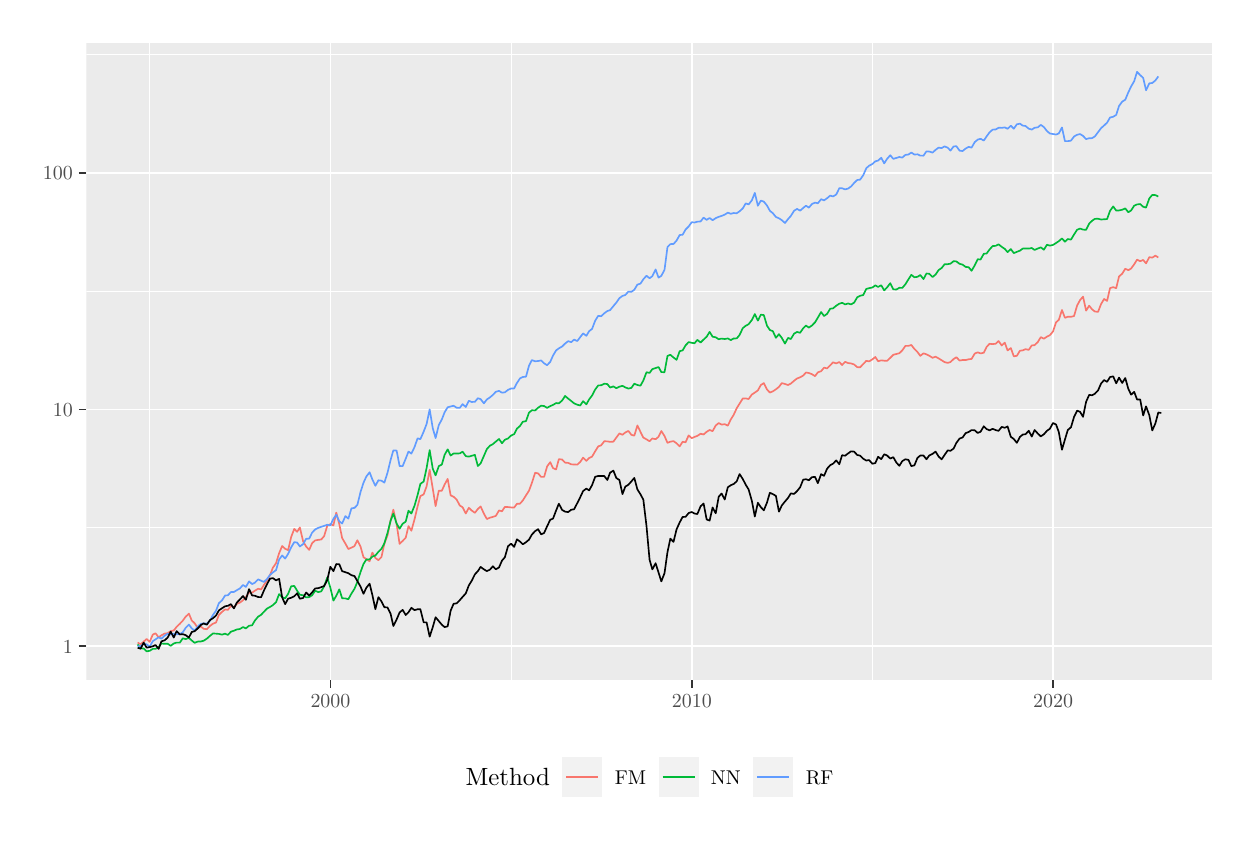
\begin{tikzpicture}[x=1pt,y=1pt]
\definecolor{fillColor}{RGB}{255,255,255}
\path[use as bounding box,fill=fillColor,fill opacity=0.00] (0,0) rectangle (433.62,289.08);
\begin{scope}
\path[clip] (  0.00,  0.00) rectangle (433.62,289.08);
\definecolor{drawColor}{RGB}{255,255,255}
\definecolor{fillColor}{RGB}{255,255,255}

\path[draw=drawColor,line width= 0.6pt,line join=round,line cap=round,fill=fillColor] (  0.00,  0.00) rectangle (433.62,289.08);
\end{scope}
\begin{scope}
\path[clip] ( 21.25, 53.26) rectangle (428.12,283.58);
\definecolor{fillColor}{gray}{0.92}

\path[fill=fillColor] ( 21.25, 53.26) rectangle (428.12,283.58);
\definecolor{drawColor}{RGB}{255,255,255}

\path[draw=drawColor,line width= 0.3pt,line join=round] ( 21.25,108.33) --
	(428.12,108.33);

\path[draw=drawColor,line width= 0.3pt,line join=round] ( 21.25,193.89) --
	(428.12,193.89);

\path[draw=drawColor,line width= 0.3pt,line join=round] ( 21.25,279.46) --
	(428.12,279.46);

\path[draw=drawColor,line width= 0.3pt,line join=round] ( 44.12, 53.26) --
	( 44.12,283.58);

\path[draw=drawColor,line width= 0.3pt,line join=round] (174.69, 53.26) --
	(174.69,283.58);

\path[draw=drawColor,line width= 0.3pt,line join=round] (305.25, 53.26) --
	(305.25,283.58);

\path[draw=drawColor,line width= 0.6pt,line join=round] ( 21.25, 65.55) --
	(428.12, 65.55);

\path[draw=drawColor,line width= 0.6pt,line join=round] ( 21.25,151.11) --
	(428.12,151.11);

\path[draw=drawColor,line width= 0.6pt,line join=round] ( 21.25,236.67) --
	(428.12,236.67);

\path[draw=drawColor,line width= 0.6pt,line join=round] (109.41, 53.26) --
	(109.41,283.58);

\path[draw=drawColor,line width= 0.6pt,line join=round] (239.98, 53.26) --
	(239.98,283.58);

\path[draw=drawColor,line width= 0.6pt,line join=round] (370.52, 53.26) --
	(370.52,283.58);
\definecolor{drawColor}{RGB}{248,118,109}

\path[draw=drawColor,line width= 0.6pt,line join=round] ( 39.74, 66.92) --
	( 40.81, 66.24) --
	( 41.92, 67.23) --
	( 42.99, 68.18) --
	( 44.07, 67.13) --
	( 45.21, 69.78) --
	( 46.21, 70.23) --
	( 47.32, 68.79) --
	( 48.32, 69.51) --
	( 49.50, 70.14) --
	( 50.57, 70.26) --
	( 51.68, 71.05) --
	( 52.79, 71.26) --
	( 53.82, 72.57) --
	( 54.97, 73.67) --
	( 56.04, 74.79) --
	( 57.08, 76.22) --
	( 58.26, 77.34) --
	( 59.29, 74.86) --
	( 60.33, 73.88) --
	( 61.47, 72.15) --
	( 62.58, 72.68) --
	( 63.58, 71.86) --
	( 64.76, 71.72) --
	( 65.84, 72.87) --
	( 66.94, 73.70) --
	( 68.05, 74.12) --
	( 69.09, 76.87) --
	( 70.23, 77.97) --
	( 71.34, 78.87) --
	( 72.34, 78.69) --
	( 73.45, 80.15) --
	( 74.52, 79.49) --
	( 75.59, 80.90) --
	( 76.70, 81.32) --
	( 77.81, 82.17) --
	( 78.85, 83.34) --
	( 79.99, 84.99) --
	( 81.10, 84.93) --
	( 82.10, 85.62) --
	( 83.28, 86.34) --
	( 84.35, 86.07) --
	( 85.35, 87.67) --
	( 86.50, 89.37) --
	( 87.57, 91.30) --
	( 88.60, 93.91) --
	( 89.75, 95.59) --
	( 90.86, 99.18) --
	( 91.96,101.78) --
	( 93.04,100.77) --
	( 94.11,100.29) --
	( 95.22,105.05) --
	( 96.33,107.97) --
	( 97.36,106.90) --
	( 98.36,108.48) --
	( 99.54,103.43) --
	(100.61,101.62) --
	(101.72,100.38) --
	(102.79,102.82) --
	(103.87,103.80) --
	(105.01,104.00) --
	(106.08,104.14) --
	(107.12,105.34) --
	(108.26,109.11) --
	(109.37,109.66) --
	(110.48,109.26) --
	(111.52,113.84) --
	(112.62,109.59) --
	(113.63,104.65) --
	(114.81,102.65) --
	(115.88,100.69) --
	(116.99,101.19) --
	(118.09,101.75) --
	(119.13,103.86) --
	(120.27,101.59) --
	(121.35, 97.72) --
	(122.38, 97.06) --
	(123.56, 96.27) --
	(124.56, 99.40) --
	(125.64, 97.45) --
	(126.74, 96.66) --
	(127.85, 97.83) --
	(128.89,102.63) --
	(130.03,105.61) --
	(131.14,111.05) --
	(132.14,114.92) --
	(133.32,109.68) --
	(134.39,102.55) --
	(135.50,103.61) --
	(136.61,104.78) --
	(137.61,108.97) --
	(138.65,107.31) --
	(139.79,111.44) --
	(140.90,116.10) --
	(141.90,119.82) --
	(143.08,120.43) --
	(144.15,123.33) --
	(145.26,129.32) --
	(146.37,122.56) --
	(147.40,116.19) --
	(148.55,121.77) --
	(149.66,121.77) --
	(150.66,123.99) --
	(151.76,126.03) --
	(152.84,120.06) --
	(153.91,119.58) --
	(155.02,118.55) --
	(156.13,116.42) --
	(157.16,115.78) --
	(158.31,113.54) --
	(159.41,115.59) --
	(160.42,114.63) --
	(161.59,113.76) --
	(162.67,115.15) --
	(163.67,116.08) --
	(164.85,113.48) --
	(165.92,111.53) --
	(167.03,112.01) --
	(168.10,112.29) --
	(169.17,112.67) --
	(170.32,114.63) --
	(171.39,114.32) --
	(172.43,115.92) --
	(173.57,115.85) --
	(174.68,115.72) --
	(175.79,115.67) --
	(176.79,117.03) --
	(177.89,117.08) --
	(178.93,118.25) --
	(180.07,120.09) --
	(181.15,121.76) --
	(182.18,124.52) --
	(183.36,128.24) --
	(184.44,128.02) --
	(185.54,126.75) --
	(186.62,126.78) --
	(187.69,130.53) --
	(188.83,132.07) --
	(189.83,129.92) --
	(190.94,129.43) --
	(191.94,133.15) --
	(193.12,133.03) --
	(194.19,131.90) --
	(195.30,131.81) --
	(196.41,131.30) --
	(197.45,131.22) --
	(198.59,131.19) --
	(199.66,132.14) --
	(200.70,133.70) --
	(201.88,132.54) --
	(202.88,133.58) --
	(203.95,134.09) --
	(205.06,136.00) --
	(206.17,137.78) --
	(207.20,138.15) --
	(208.35,139.62) --
	(209.46,139.59) --
	(210.46,139.41) --
	(211.64,139.49) --
	(212.71,140.97) --
	(213.82,142.46) --
	(214.93,141.97) --
	(215.96,142.81) --
	(217.07,143.35) --
	(218.14,141.96) --
	(219.21,141.65) --
	(220.32,145.35) --
	(221.43,143.03) --
	(222.47,140.95) --
	(223.61,140.32) --
	(224.72,139.63) --
	(225.72,140.64) --
	(226.90,140.37) --
	(227.97,141.26) --
	(228.97,143.33) --
	(230.12,141.53) --
	(231.19,139.05) --
	(232.23,139.47) --
	(233.37,139.68) --
	(234.48,138.89) --
	(235.59,137.77) --
	(236.66,139.45) --
	(237.73,139.25) --
	(238.84,141.75) --
	(239.95,140.74) --
	(240.98,141.20) --
	(241.98,141.58) --
	(243.16,142.34) --
	(244.24,142.08) --
	(245.34,143.04) --
	(246.42,143.71) --
	(247.49,143.28) --
	(248.63,145.34) --
	(249.70,146.20) --
	(250.74,145.65) --
	(251.89,145.79) --
	(252.99,145.28) --
	(254.10,147.56) --
	(255.10,149.16) --
	(256.21,151.56) --
	(257.25,153.24) --
	(258.39,155.07) --
	(259.46,155.12) --
	(260.50,154.88) --
	(261.68,156.52) --
	(262.75,157.21) --
	(263.86,158.01) --
	(264.93,159.95) --
	(266.00,160.66) --
	(267.15,158.34) --
	(268.18,157.23) --
	(269.26,157.66) --
	(270.37,158.40) --
	(271.47,159.27) --
	(272.51,160.64) --
	(273.65,160.33) --
	(274.76,159.95) --
	(275.76,160.47) --
	(276.94,161.49) --
	(278.01,162.31) --
	(279.12,162.74) --
	(280.23,163.37) --
	(281.23,164.47) --
	(282.27,164.30) --
	(283.41,163.85) --
	(284.52,163.16) --
	(285.52,164.52) --
	(286.70,164.95) --
	(287.77,166.23) --
	(288.88,165.95) --
	(289.99,167.08) --
	(291.03,168.16) --
	(292.17,167.76) --
	(293.28,168.26) --
	(294.28,167.18) --
	(295.39,168.33) --
	(296.46,167.88) --
	(297.53,167.76) --
	(298.64,167.37) --
	(299.75,166.41) --
	(300.78,166.33) --
	(301.93,167.55) --
	(303.04,168.69) --
	(304.04,168.48) --
	(305.22,169.22) --
	(306.29,170.08) --
	(307.29,168.54) --
	(308.43,168.87) --
	(309.51,168.74) --
	(310.54,168.69) --
	(311.69,169.77) --
	(312.79,170.88) --
	(313.90,171.16) --
	(314.97,171.44) --
	(316.05,172.48) --
	(317.15,174.08) --
	(318.26,174.09) --
	(319.30,174.43) --
	(320.41,172.98) --
	(321.52,171.87) --
	(322.55,170.48) --
	(323.70,171.41) --
	(324.77,171.04) --
	(325.80,170.51) --
	(326.98,169.79) --
	(328.06,170.19) --
	(329.16,169.58) --
	(330.24,168.91) --
	(331.31,168.23) --
	(332.45,167.94) --
	(333.45,168.27) --
	(334.56,169.32) --
	(335.56,170.00) --
	(336.74,168.80) --
	(337.82,168.98) --
	(338.92,168.96) --
	(340.03,169.25) --
	(341.07,169.38) --
	(342.21,171.31) --
	(343.28,171.77) --
	(344.32,171.37) --
	(345.50,171.62) --
	(346.50,173.71) --
	(347.57,174.85) --
	(348.68,174.73) --
	(349.79,174.87) --
	(350.83,175.83) --
	(351.97,174.24) --
	(353.08,175.26) --
	(354.08,172.44) --
	(355.26,173.31) --
	(356.33,170.32) --
	(357.44,170.50) --
	(358.55,172.35) --
	(359.55,172.47) --
	(360.58,172.91) --
	(361.73,172.65) --
	(362.84,174.27) --
	(363.84,174.35) --
	(365.02,175.49) --
	(366.09,177.26) --
	(367.20,176.67) --
	(368.31,177.43) --
	(369.34,177.92) --
	(370.49,179.28) --
	(371.59,182.60) --
	(372.59,183.49) --
	(373.74,187.05) --
	(374.81,184.24) --
	(375.85,184.62) --
	(376.99,184.59) --
	(378.10,184.87) --
	(379.21,188.67) --
	(380.28,190.65) --
	(381.35,191.89) --
	(382.46,186.83) --
	(383.57,188.62) --
	(384.60,187.31) --
	(385.61,186.51) --
	(386.79,186.40) --
	(387.86,189.20) --
	(388.97,191.04) --
	(390.04,190.32) --
	(391.11,194.96) --
	(392.25,195.32) --
	(393.33,194.93) --
	(394.36,199.18) --
	(395.51,200.18) --
	(396.61,201.97) --
	(397.72,201.44) --
	(398.72,202.05) --
	(399.83,203.57) --
	(400.87,205.24) --
	(402.01,204.68) --
	(403.08,205.15) --
	(404.12,203.91) --
	(405.30,206.15) --
	(406.37,205.98) --
	(407.48,206.69) --
	(408.55,206.06);
\definecolor{drawColor}{RGB}{0,186,56}

\path[draw=drawColor,line width= 0.6pt,line join=round] ( 39.74, 66.21) --
	( 40.81, 64.80) --
	( 41.92, 64.74) --
	( 42.99, 63.73) --
	( 44.07, 63.91) --
	( 45.21, 64.60) --
	( 46.21, 64.60) --
	( 47.32, 65.21) --
	( 48.32, 66.56) --
	( 49.50, 66.43) --
	( 50.57, 66.48) --
	( 51.68, 65.71) --
	( 52.79, 66.56) --
	( 53.82, 66.88) --
	( 54.97, 66.85) --
	( 56.04, 68.43) --
	( 57.08, 68.14) --
	( 58.26, 68.56) --
	( 59.29, 67.64) --
	( 60.33, 66.80) --
	( 61.47, 67.24) --
	( 62.58, 67.29) --
	( 63.58, 67.54) --
	( 64.76, 68.31) --
	( 65.84, 69.28) --
	( 66.94, 70.17) --
	( 68.05, 70.11) --
	( 69.09, 70.01) --
	( 70.23, 69.75) --
	( 71.34, 70.11) --
	( 72.34, 69.64) --
	( 73.45, 70.83) --
	( 74.52, 71.17) --
	( 75.59, 71.62) --
	( 76.70, 71.79) --
	( 77.81, 72.49) --
	( 78.85, 72.01) --
	( 79.99, 72.97) --
	( 81.10, 73.13) --
	( 82.10, 74.83) --
	( 83.28, 76.26) --
	( 84.35, 76.91) --
	( 85.35, 77.99) --
	( 86.50, 79.18) --
	( 87.57, 79.75) --
	( 88.60, 80.42) --
	( 89.75, 81.48) --
	( 90.86, 84.41) --
	( 91.96, 83.28) --
	( 93.04, 82.88) --
	( 94.11, 84.50) --
	( 95.22, 87.22) --
	( 96.33, 87.35) --
	( 97.36, 85.63) --
	( 98.36, 84.15) --
	( 99.54, 84.00) --
	(100.61, 83.21) --
	(101.72, 83.31) --
	(102.79, 83.98) --
	(103.87, 85.63) --
	(105.01, 85.11) --
	(106.08, 85.39) --
	(107.12, 87.22) --
	(108.26, 90.43) --
	(109.37, 86.73) --
	(110.48, 82.04) --
	(111.52, 83.82) --
	(112.62, 86.12) --
	(113.63, 82.90) --
	(114.81, 82.84) --
	(115.88, 82.55) --
	(116.99, 84.59) --
	(118.09, 86.30) --
	(119.13, 88.80) --
	(120.27, 92.36) --
	(121.35, 95.30) --
	(122.38, 96.90) --
	(123.56, 96.95) --
	(124.56, 97.97) --
	(125.64, 98.33) --
	(126.74, 99.70) --
	(127.85,100.76) --
	(128.89,102.79) --
	(130.03,106.51) --
	(131.14,110.90) --
	(132.14,113.50) --
	(133.32,109.88) --
	(134.39,108.04) --
	(135.50,109.83) --
	(136.61,110.60) --
	(137.61,114.54) --
	(138.65,113.52) --
	(139.79,116.36) --
	(140.90,120.23) --
	(141.90,124.23) --
	(143.08,125.07) --
	(144.15,129.94) --
	(145.26,136.44) --
	(146.37,129.72) --
	(147.40,127.30) --
	(148.55,130.63) --
	(149.66,131.22) --
	(150.66,134.73) --
	(151.76,136.70) --
	(152.84,134.47) --
	(153.91,135.21) --
	(155.02,135.22) --
	(156.13,135.24) --
	(157.16,135.86) --
	(158.31,134.25) --
	(159.41,134.07) --
	(160.42,134.37) --
	(161.59,134.70) --
	(162.67,130.69) --
	(163.67,131.61) --
	(164.85,134.32) --
	(165.92,136.80) --
	(167.03,138.02) --
	(168.10,138.60) --
	(169.17,139.52) --
	(170.32,140.45) --
	(171.39,138.90) --
	(172.43,140.18) --
	(173.57,140.63) --
	(174.68,141.70) --
	(175.79,142.21) --
	(176.79,144.18) --
	(177.89,145.15) --
	(178.93,146.69) --
	(180.07,146.90) --
	(181.15,149.97) --
	(182.18,150.83) --
	(183.36,150.76) --
	(184.44,151.75) --
	(185.54,152.48) --
	(186.62,152.35) --
	(187.69,151.71) --
	(188.83,152.34) --
	(189.83,152.76) --
	(190.94,153.43) --
	(191.94,153.31) --
	(193.12,154.36) --
	(194.19,155.99) --
	(195.30,155.05) --
	(196.41,154.18) --
	(197.45,153.33) --
	(198.59,152.84) --
	(199.66,152.55) --
	(200.70,154.11) --
	(201.88,152.97) --
	(202.88,154.76) --
	(203.95,156.17) --
	(205.06,158.31) --
	(206.17,159.81) --
	(207.20,159.85) --
	(208.35,160.42) --
	(209.46,160.30) --
	(210.46,159.04) --
	(211.64,159.45) --
	(212.71,158.80) --
	(213.82,159.34) --
	(214.93,159.66) --
	(215.96,159.09) --
	(217.07,158.67) --
	(218.14,158.92) --
	(219.21,160.42) --
	(220.32,159.96) --
	(221.43,159.71) --
	(222.47,161.58) --
	(223.61,164.57) --
	(224.72,164.32) --
	(225.72,165.70) --
	(226.90,166.07) --
	(227.97,166.45) --
	(228.97,164.61) --
	(230.12,164.58) --
	(231.19,170.47) --
	(232.23,170.87) --
	(233.37,169.89) --
	(234.48,169.06) --
	(235.59,172.17) --
	(236.66,172.46) --
	(237.73,174.28) --
	(238.84,175.46) --
	(239.95,175.20) --
	(240.98,175.05) --
	(241.98,176.27) --
	(243.16,175.31) --
	(244.24,176.37) --
	(245.34,177.39) --
	(246.42,179.15) --
	(247.49,177.41) --
	(248.63,177.18) --
	(249.70,176.49) --
	(250.74,176.73) --
	(251.89,176.57) --
	(252.99,176.78) --
	(254.10,176.20) --
	(255.10,176.77) --
	(256.21,176.80) --
	(257.25,178.04) --
	(258.39,180.49) --
	(259.46,181.36) --
	(260.50,181.92) --
	(261.68,183.44) --
	(262.75,185.60) --
	(263.86,183.22) --
	(264.93,185.37) --
	(266.00,185.23) --
	(267.15,181.40) --
	(268.18,179.83) --
	(269.26,179.41) --
	(270.37,177.01) --
	(271.47,178.32) --
	(272.51,176.96) --
	(273.65,174.92) --
	(274.76,176.98) --
	(275.76,176.56) --
	(276.94,178.51) --
	(278.01,179.13) --
	(279.12,178.82) --
	(280.23,180.47) --
	(281.23,181.42) --
	(282.27,180.71) --
	(283.41,181.48) --
	(284.52,182.60) --
	(285.52,184.29) --
	(286.70,186.33) --
	(287.77,184.87) --
	(288.88,185.68) --
	(289.99,187.52) --
	(291.03,187.65) --
	(292.17,188.62) --
	(293.28,189.33) --
	(294.28,189.66) --
	(295.39,189.08) --
	(296.46,189.42) --
	(297.53,189.09) --
	(298.64,189.73) --
	(299.75,191.64) --
	(300.78,192.20) --
	(301.93,192.46) --
	(303.04,194.66) --
	(304.04,194.96) --
	(305.22,195.18) --
	(306.29,195.95) --
	(307.29,195.40) --
	(308.43,195.99) --
	(309.51,194.15) --
	(310.54,195.21) --
	(311.69,196.75) --
	(312.79,194.54) --
	(313.90,194.46) --
	(314.97,195.08) --
	(316.05,195.05) --
	(317.15,196.35) --
	(318.26,198.13) --
	(319.30,199.76) --
	(320.41,198.90) --
	(321.52,199.04) --
	(322.55,199.70) --
	(323.70,198.23) --
	(324.77,200.24) --
	(325.80,200.15) --
	(326.98,198.97) --
	(328.06,199.87) --
	(329.16,201.48) --
	(330.24,202.21) --
	(331.31,203.57) --
	(332.45,203.62) --
	(333.45,203.80) --
	(334.56,204.69) --
	(335.56,204.62) --
	(336.74,203.74) --
	(337.82,203.46) --
	(338.92,202.63) --
	(340.03,202.52) --
	(341.07,201.24) --
	(342.21,203.17) --
	(343.28,205.39) --
	(344.32,205.31) --
	(345.50,207.39) --
	(346.50,207.46) --
	(347.57,208.92) --
	(348.68,210.16) --
	(349.79,210.24) --
	(350.83,210.78) --
	(351.97,209.89) --
	(353.08,209.13) --
	(354.08,207.98) --
	(355.26,209.07) --
	(356.33,207.62) --
	(357.44,208.07) --
	(358.55,208.51) --
	(359.55,209.25) --
	(360.58,209.31) --
	(361.73,209.25) --
	(362.84,209.45) --
	(363.84,208.76) --
	(365.02,209.28) --
	(366.09,209.69) --
	(367.20,208.85) --
	(368.31,210.63) --
	(369.34,210.33) --
	(370.49,210.56) --
	(371.59,211.25) --
	(372.59,211.91) --
	(373.74,212.93) --
	(374.81,211.74) --
	(375.85,212.70) --
	(376.99,212.49) --
	(378.10,214.34) --
	(379.21,216.05) --
	(380.28,216.49) --
	(381.35,216.11) --
	(382.46,216.03) --
	(383.57,218.29) --
	(384.60,219.28) --
	(385.61,219.99) --
	(386.79,220.03) --
	(387.86,219.75) --
	(388.97,219.84) --
	(390.04,219.92) --
	(391.11,222.90) --
	(392.25,224.48) --
	(393.33,222.99) --
	(394.36,223.04) --
	(395.51,223.29) --
	(396.61,223.77) --
	(397.72,222.39) --
	(398.72,223.02) --
	(399.83,224.75) --
	(400.87,225.21) --
	(402.01,225.34) --
	(403.08,224.36) --
	(404.12,224.07) --
	(405.30,227.38) --
	(406.37,228.65) --
	(407.48,228.58) --
	(408.55,228.04);
\definecolor{drawColor}{RGB}{97,156,255}

\path[draw=drawColor,line width= 0.6pt,line join=round] ( 39.74, 65.55) --
	( 40.81, 65.58) --
	( 41.92, 66.42) --
	( 42.99, 66.24) --
	( 44.07, 65.41) --
	( 45.21, 67.38) --
	( 46.21, 68.07) --
	( 47.32, 68.77) --
	( 48.32, 68.30) --
	( 49.50, 69.37) --
	( 50.57, 70.08) --
	( 51.68, 69.80) --
	( 52.79, 70.08) --
	( 53.82, 69.86) --
	( 54.97, 69.99) --
	( 56.04, 70.57) --
	( 57.08, 72.19) --
	( 58.26, 73.39) --
	( 59.29, 72.01) --
	( 60.33, 71.27) --
	( 61.47, 72.71) --
	( 62.58, 73.69) --
	( 63.58, 73.79) --
	( 64.76, 73.78) --
	( 65.84, 74.76) --
	( 66.94, 76.83) --
	( 68.05, 78.38) --
	( 69.09, 81.12) --
	( 70.23, 82.14) --
	( 71.34, 83.90) --
	( 72.34, 83.97) --
	( 73.45, 85.14) --
	( 74.52, 85.16) --
	( 75.59, 85.83) --
	( 76.70, 86.45) --
	( 77.81, 87.71) --
	( 78.85, 86.99) --
	( 79.99, 88.99) --
	( 81.10, 88.02) --
	( 82.10, 88.52) --
	( 83.28, 89.72) --
	( 84.35, 89.26) --
	( 85.35, 88.79) --
	( 86.50, 89.88) --
	( 87.57, 91.31) --
	( 88.60, 92.23) --
	( 89.75, 93.06) --
	( 90.86, 96.89) --
	( 91.96, 98.37) --
	( 93.04, 97.24) --
	( 94.11, 98.94) --
	( 95.22,101.31) --
	( 96.33,103.18) --
	( 97.36,103.03) --
	( 98.36,101.61) --
	( 99.54,102.48) --
	(100.61,104.37) --
	(101.72,104.45) --
	(102.79,106.63) --
	(103.87,107.75) --
	(105.01,108.32) --
	(106.08,108.73) --
	(107.12,109.04) --
	(108.26,109.46) --
	(109.37,109.22) --
	(110.48,111.62) --
	(111.52,113.06) --
	(112.62,110.67) --
	(113.63,109.91) --
	(114.81,112.59) --
	(115.88,111.67) --
	(116.99,115.38) --
	(118.09,115.55) --
	(119.13,116.62) --
	(120.27,121.27) --
	(121.35,124.64) --
	(122.38,126.91) --
	(123.56,128.41) --
	(124.56,125.81) --
	(125.64,123.54) --
	(126.74,125.53) --
	(127.85,125.38) --
	(128.89,124.68) --
	(130.03,128.27) --
	(131.14,132.86) --
	(132.14,136.35) --
	(133.32,136.25) --
	(134.39,130.68) --
	(135.50,130.64) --
	(136.61,133.37) --
	(137.61,135.91) --
	(138.65,135.16) --
	(139.79,137.55) --
	(140.90,140.69) --
	(141.90,140.39) --
	(143.08,143.09) --
	(144.15,145.86) --
	(145.26,151.15) --
	(146.37,144.38) --
	(147.40,140.79) --
	(148.55,145.46) --
	(149.66,147.53) --
	(150.66,150.09) --
	(151.76,151.91) --
	(152.84,152.20) --
	(153.91,152.46) --
	(155.02,151.73) --
	(156.13,151.69) --
	(157.16,153.03) --
	(158.31,152.01) --
	(159.41,154.26) --
	(160.42,153.83) --
	(161.59,153.87) --
	(162.67,155.17) --
	(163.67,154.85) --
	(164.85,153.34) --
	(165.92,154.72) --
	(167.03,155.47) --
	(168.10,156.39) --
	(169.17,157.51) --
	(170.32,157.83) --
	(171.39,157.18) --
	(172.43,157.31) --
	(173.57,158.19) --
	(174.68,158.71) --
	(175.79,158.72) --
	(176.79,160.68) --
	(177.89,162.34) --
	(178.93,162.85) --
	(180.07,162.97) --
	(181.15,166.92) --
	(182.18,168.95) --
	(183.36,168.53) --
	(184.44,168.62) --
	(185.54,168.83) --
	(186.62,167.79) --
	(187.69,167.12) --
	(188.83,168.33) --
	(189.83,170.59) --
	(190.94,172.46) --
	(191.94,173.20) --
	(193.12,173.87) --
	(194.19,174.93) --
	(195.30,175.79) --
	(196.41,175.45) --
	(197.45,176.36) --
	(198.59,175.84) --
	(199.66,177.25) --
	(200.70,178.60) --
	(201.88,177.74) --
	(202.88,179.41) --
	(203.95,180.24) --
	(205.06,183.19) --
	(206.17,184.96) --
	(207.20,184.80) --
	(208.35,185.86) --
	(209.46,186.69) --
	(210.46,187.02) --
	(211.64,188.46) --
	(212.71,189.73) --
	(213.82,191.34) --
	(214.93,192.15) --
	(215.96,192.50) --
	(217.07,193.71) --
	(218.14,193.62) --
	(219.21,194.38) --
	(220.32,196.23) --
	(221.43,196.59) --
	(222.47,198.17) --
	(223.61,199.43) --
	(224.72,198.54) --
	(225.72,199.27) --
	(226.90,201.71) --
	(227.97,198.73) --
	(228.97,199.41) --
	(230.12,201.58) --
	(231.19,209.80) --
	(232.23,210.87) --
	(233.37,210.91) --
	(234.48,212.16) --
	(235.59,214.14) --
	(236.66,214.25) --
	(237.73,216.14) --
	(238.84,217.24) --
	(239.95,218.78) --
	(240.98,218.68) --
	(241.98,218.97) --
	(243.16,219.05) --
	(244.24,220.44) --
	(245.34,219.63) --
	(246.42,220.32) --
	(247.49,219.51) --
	(248.63,220.26) --
	(249.70,220.72) --
	(250.74,221.05) --
	(251.89,221.53) --
	(252.99,222.22) --
	(254.10,221.83) --
	(255.10,222.10) --
	(256.21,222.02) --
	(257.25,222.74) --
	(258.39,223.76) --
	(259.46,225.59) --
	(260.50,225.21) --
	(261.68,226.68) --
	(262.75,229.39) --
	(263.86,224.74) --
	(264.93,226.59) --
	(266.00,226.21) --
	(267.15,224.82) --
	(268.18,222.93) --
	(269.26,222.04) --
	(270.37,220.68) --
	(271.47,220.20) --
	(272.51,219.51) --
	(273.65,218.51) --
	(274.76,219.91) --
	(275.76,221.04) --
	(276.94,222.92) --
	(278.01,223.58) --
	(279.12,222.96) --
	(280.23,223.92) --
	(281.23,224.75) --
	(282.27,224.04) --
	(283.41,225.36) --
	(284.52,225.87) --
	(285.52,225.62) --
	(286.70,227.09) --
	(287.77,226.68) --
	(288.88,227.45) --
	(289.99,228.40) --
	(291.03,228.09) --
	(292.17,228.79) --
	(293.28,231.06) --
	(294.28,231.05) --
	(295.39,230.63) --
	(296.46,230.95) --
	(297.53,231.68) --
	(298.64,232.98) --
	(299.75,234.04) --
	(300.78,234.14) --
	(301.93,235.77) --
	(303.04,238.31) --
	(304.04,239.18) --
	(305.22,239.81) --
	(306.29,240.78) --
	(307.29,241.05) --
	(308.43,242.07) --
	(309.51,240.04) --
	(310.54,241.67) --
	(311.69,242.98) --
	(312.79,241.67) --
	(313.90,242.01) --
	(314.97,242.35) --
	(316.05,242.14) --
	(317.15,243.10) --
	(318.26,243.24) --
	(319.30,243.96) --
	(320.41,243.23) --
	(321.52,243.32) --
	(322.55,242.85) --
	(323.70,242.82) --
	(324.77,244.39) --
	(325.80,244.31) --
	(326.98,243.94) --
	(328.06,244.92) --
	(329.16,245.73) --
	(330.24,245.56) --
	(331.31,246.18) --
	(332.45,245.71) --
	(333.45,244.65) --
	(334.56,246.12) --
	(335.56,246.27) --
	(336.74,244.64) --
	(337.82,244.50) --
	(338.92,245.39) --
	(340.03,246.02) --
	(341.07,245.73) --
	(342.21,247.71) --
	(343.28,248.62) --
	(344.32,248.92) --
	(345.50,248.30) --
	(346.50,249.79) --
	(347.57,251.25) --
	(348.68,252.23) --
	(349.79,252.29) --
	(350.83,252.90) --
	(351.97,252.88) --
	(353.08,253.03) --
	(354.08,252.54) --
	(355.26,253.64) --
	(356.33,252.57) --
	(357.44,254.17) --
	(358.55,254.38) --
	(359.55,253.70) --
	(360.58,253.54) --
	(361.73,252.58) --
	(362.84,252.26) --
	(363.84,252.91) --
	(365.02,253.08) --
	(366.09,253.94) --
	(367.20,253.17) --
	(368.31,251.73) --
	(369.34,250.85) --
	(370.49,250.65) --
	(371.59,250.46) --
	(372.59,250.85) --
	(373.74,253.02) --
	(374.81,248.07) --
	(375.85,248.08) --
	(376.99,248.25) --
	(378.10,249.75) --
	(379.21,250.38) --
	(380.28,250.64) --
	(381.35,249.97) --
	(382.46,248.80) --
	(383.57,249.14) --
	(384.60,249.15) --
	(385.61,249.77) --
	(386.79,251.32) --
	(387.86,252.75) --
	(388.97,253.75) --
	(390.04,254.75) --
	(391.11,256.61) --
	(392.25,256.89) --
	(393.33,257.55) --
	(394.36,260.79) --
	(395.51,262.36) --
	(396.61,263.04) --
	(397.72,265.72) --
	(398.72,267.82) --
	(399.83,269.74) --
	(400.87,273.11) --
	(402.01,271.92) --
	(403.08,270.93) --
	(404.12,266.47) --
	(405.30,268.96) --
	(406.37,269.09) --
	(407.48,269.99) --
	(408.55,271.46);
\definecolor{drawColor}{RGB}{0,0,0}

\path[draw=drawColor,line width= 0.6pt,line join=round] ( 39.74, 65.03) --
	( 40.81, 64.65) --
	( 41.92, 66.86) --
	( 42.99, 65.04) --
	( 44.07, 65.24) --
	( 45.21, 65.55) --
	( 46.21, 65.99) --
	( 47.32, 64.60) --
	( 48.32, 67.32) --
	( 49.50, 67.71) --
	( 50.57, 68.67) --
	( 51.68, 70.84) --
	( 52.79, 68.70) --
	( 53.82, 71.03) --
	( 54.97, 69.82) --
	( 56.04, 69.91) --
	( 57.08, 69.57) --
	( 58.26, 68.70) --
	( 59.29, 70.73) --
	( 60.33, 71.00) --
	( 61.47, 72.01) --
	( 62.58, 73.22) --
	( 63.58, 73.80) --
	( 64.76, 73.34) --
	( 65.84, 74.98) --
	( 66.94, 75.68) --
	( 68.05, 76.64) --
	( 69.09, 78.49) --
	( 70.23, 79.30) --
	( 71.34, 80.01) --
	( 72.34, 80.18) --
	( 73.45, 80.77) --
	( 74.52, 79.23) --
	( 75.59, 81.34) --
	( 76.70, 82.49) --
	( 77.81, 83.69) --
	( 78.85, 82.36) --
	( 79.99, 86.19) --
	( 81.10, 83.93) --
	( 82.10, 83.81) --
	( 83.28, 83.34) --
	( 84.35, 83.28) --
	( 85.35, 85.65) --
	( 86.50, 88.04) --
	( 87.57, 89.98) --
	( 88.60, 90.18) --
	( 89.75, 89.37) --
	( 90.86, 89.90) --
	( 91.96, 83.21) --
	( 93.04, 80.77) --
	( 94.11, 82.75) --
	( 95.22, 83.08) --
	( 96.33, 83.62) --
	( 97.36, 84.69) --
	( 98.36, 82.73) --
	( 99.54, 83.00) --
	(100.61, 84.97) --
	(101.72, 83.87) --
	(102.79, 85.02) --
	(103.87, 86.43) --
	(105.01, 86.56) --
	(106.08, 86.92) --
	(107.12, 87.31) --
	(108.26, 89.48) --
	(109.37, 94.28) --
	(110.48, 92.70) --
	(111.52, 95.26) --
	(112.62, 95.17) --
	(113.63, 92.68) --
	(114.81, 92.32) --
	(115.88, 91.95) --
	(116.99, 91.23) --
	(118.09, 90.92) --
	(119.13, 89.11) --
	(120.27, 87.13) --
	(121.35, 84.50) --
	(122.38, 86.70) --
	(123.56, 88.16) --
	(124.56, 84.05) --
	(125.64, 78.94) --
	(126.74, 83.29) --
	(127.85, 81.76) --
	(128.89, 79.66) --
	(130.03, 79.57) --
	(131.14, 77.31) --
	(132.14, 72.86) --
	(133.32, 75.24) --
	(134.39, 77.75) --
	(135.50, 78.70) --
	(136.61, 76.84) --
	(137.61, 77.84) --
	(138.65, 79.45) --
	(139.79, 78.60) --
	(140.90, 78.93) --
	(141.90, 78.95) --
	(143.08, 74.21) --
	(144.15, 74.16) --
	(145.26, 69.02) --
	(146.37, 72.43) --
	(147.40, 76.04) --
	(148.55, 74.66) --
	(149.66, 73.34) --
	(150.66, 72.47) --
	(151.76, 72.76) --
	(152.84, 78.42) --
	(153.91, 80.91) --
	(155.02, 81.07) --
	(156.13, 82.19) --
	(157.16, 83.39) --
	(158.31, 84.65) --
	(159.41, 87.54) --
	(160.42, 89.17) --
	(161.59, 91.52) --
	(162.67, 92.70) --
	(163.67, 94.22) --
	(164.85, 93.35) --
	(165.92, 92.71) --
	(167.03, 93.24) --
	(168.10, 94.45) --
	(169.17, 93.36) --
	(170.32, 94.03) --
	(171.39, 96.50) --
	(172.43, 97.69) --
	(173.57,101.69) --
	(174.68,102.63) --
	(175.79,101.46) --
	(176.79,104.18) --
	(177.89,103.40) --
	(178.93,102.41) --
	(180.07,103.15) --
	(181.15,104.07) --
	(182.18,105.89) --
	(183.36,107.15) --
	(184.44,107.85) --
	(185.54,105.99) --
	(186.62,106.50) --
	(187.69,108.89) --
	(188.83,111.28) --
	(189.83,111.66) --
	(190.94,114.60) --
	(191.94,117.07) --
	(193.12,114.81) --
	(194.19,114.20) --
	(195.30,114.03) --
	(196.41,114.89) --
	(197.45,115.05) --
	(198.59,117.27) --
	(199.66,119.41) --
	(200.70,121.64) --
	(201.88,122.52) --
	(202.88,121.87) --
	(203.95,123.81) --
	(205.06,126.76) --
	(206.17,127.11) --
	(207.20,127.06) --
	(208.35,127.06) --
	(209.46,125.64) --
	(210.46,128.29) --
	(211.64,129.01) --
	(212.71,126.35) --
	(213.82,125.63) --
	(214.93,120.54) --
	(215.96,123.24) --
	(217.07,123.92) --
	(218.14,125.12) --
	(219.21,126.39) --
	(220.32,122.23) --
	(221.43,120.48) --
	(222.47,118.52) --
	(223.61,108.99) --
	(224.72, 96.83) --
	(225.72, 93.32) --
	(226.90, 95.56) --
	(227.97, 92.17) --
	(228.97, 88.99) --
	(230.12, 91.97) --
	(231.19, 99.58) --
	(232.23,104.44) --
	(233.37,103.27) --
	(234.48,107.82) --
	(235.59,110.28) --
	(236.66,112.28) --
	(237.73,112.31) --
	(238.84,113.69) --
	(239.95,114.06) --
	(240.98,113.52) --
	(241.98,113.32) --
	(243.16,116.13) --
	(244.24,117.15) --
	(245.34,111.37) --
	(246.42,110.96) --
	(247.49,115.68) --
	(248.63,113.60) --
	(249.70,119.58) --
	(250.74,120.74) --
	(251.89,118.58) --
	(252.99,122.99) --
	(254.10,123.76) --
	(255.10,124.18) --
	(256.21,125.15) --
	(257.25,127.77) --
	(258.39,126.01) --
	(259.46,123.93) --
	(260.50,122.23) --
	(261.68,118.10) --
	(262.75,112.43) --
	(263.86,117.39) --
	(264.93,115.81) --
	(266.00,114.66) --
	(267.15,117.48) --
	(268.18,121.02) --
	(269.26,120.54) --
	(270.37,119.89) --
	(271.47,114.19) --
	(272.51,116.44) --
	(273.65,117.86) --
	(274.76,119.15) --
	(275.76,120.80) --
	(276.94,120.59) --
	(278.01,121.62) --
	(279.12,122.99) --
	(280.23,125.76) --
	(281.23,125.90) --
	(282.27,125.54) --
	(283.41,126.66) --
	(284.52,126.74) --
	(285.52,124.49) --
	(286.70,127.73) --
	(287.77,127.14) --
	(288.88,129.74) --
	(289.99,130.98) --
	(291.03,131.54) --
	(292.17,132.72) --
	(293.28,131.33) --
	(294.28,134.59) --
	(295.39,134.41) --
	(296.46,135.24) --
	(297.53,135.99) --
	(298.64,135.88) --
	(299.75,134.67) --
	(300.78,134.44) --
	(301.93,133.30) --
	(303.04,132.66) --
	(304.04,132.84) --
	(305.22,131.51) --
	(306.29,131.73) --
	(307.29,134.02) --
	(308.43,133.17) --
	(309.51,134.93) --
	(310.54,134.49) --
	(311.69,133.38) --
	(312.79,133.88) --
	(313.90,131.93) --
	(314.97,130.75) --
	(316.05,132.47) --
	(317.15,133.12) --
	(318.26,132.90) --
	(319.30,130.65) --
	(320.41,130.92) --
	(321.52,133.62) --
	(322.55,134.47) --
	(323.70,134.46) --
	(324.77,133.12) --
	(325.80,134.50) --
	(326.98,135.07) --
	(328.06,135.90) --
	(329.16,134.13) --
	(330.24,133.09) --
	(331.31,134.66) --
	(332.45,136.34) --
	(333.45,136.18) --
	(334.56,136.97) --
	(335.56,139.01) --
	(336.74,140.61) --
	(337.82,140.99) --
	(338.92,142.55) --
	(340.03,142.99) --
	(341.07,143.66) --
	(342.21,143.61) --
	(343.28,142.62) --
	(344.32,143.08) --
	(345.50,145.05) --
	(346.50,144.05) --
	(347.57,143.57) --
	(348.68,144.13) --
	(349.79,143.66) --
	(350.83,143.40) --
	(351.97,144.82) --
	(353.08,144.50) --
	(354.08,145.00) --
	(355.26,141.23) --
	(356.33,140.45) --
	(357.44,139.06) --
	(358.55,141.19) --
	(359.55,142.04) --
	(360.58,142.18) --
	(361.73,143.42) --
	(362.84,141.32) --
	(363.84,143.70) --
	(365.02,142.41) --
	(366.09,141.39) --
	(367.20,142.14) --
	(368.31,143.41) --
	(369.34,144.11) --
	(370.49,146.21) --
	(371.59,145.71) --
	(372.59,142.96) --
	(373.74,136.57) --
	(374.81,140.24) --
	(375.85,143.71) --
	(376.99,144.68) --
	(378.10,148.41) --
	(379.21,150.69) --
	(380.28,150.26) --
	(381.35,148.46) --
	(382.46,153.90) --
	(383.57,156.38) --
	(384.60,156.25) --
	(385.61,156.79) --
	(386.79,158.02) --
	(387.86,160.48) --
	(388.97,161.74) --
	(390.04,161.11) --
	(391.11,162.83) --
	(392.25,163.09) --
	(393.33,160.56) --
	(394.36,162.62) --
	(395.51,160.70) --
	(396.61,162.48) --
	(397.72,158.56) --
	(398.72,156.46) --
	(399.83,157.49) --
	(400.87,154.72) --
	(402.01,154.70) --
	(403.08,148.95) --
	(404.12,152.24) --
	(405.30,149.03) --
	(406.37,143.54) --
	(407.48,146.04) --
	(408.55,150.02) --
	(409.63,149.84);
\end{scope}
\begin{scope}
\path[clip] (  0.00,  0.00) rectangle (433.62,289.08);
\definecolor{drawColor}{gray}{0.30}

\node[text=drawColor,anchor=base east,inner sep=0pt, outer sep=0pt, scale=  0.72] at ( 16.30, 63.07) {1};

\node[text=drawColor,anchor=base east,inner sep=0pt, outer sep=0pt, scale=  0.72] at ( 16.30,148.63) {10};

\node[text=drawColor,anchor=base east,inner sep=0pt, outer sep=0pt, scale=  0.72] at ( 16.30,234.20) {100};
\end{scope}
\begin{scope}
\path[clip] (  0.00,  0.00) rectangle (433.62,289.08);
\definecolor{drawColor}{gray}{0.20}

\path[draw=drawColor,line width= 0.6pt,line join=round] ( 18.50, 65.55) --
	( 21.25, 65.55);

\path[draw=drawColor,line width= 0.6pt,line join=round] ( 18.50,151.11) --
	( 21.25,151.11);

\path[draw=drawColor,line width= 0.6pt,line join=round] ( 18.50,236.67) --
	( 21.25,236.67);
\end{scope}
\begin{scope}
\path[clip] (  0.00,  0.00) rectangle (433.62,289.08);
\definecolor{drawColor}{gray}{0.20}

\path[draw=drawColor,line width= 0.6pt,line join=round] (109.41, 50.51) --
	(109.41, 53.26);

\path[draw=drawColor,line width= 0.6pt,line join=round] (239.98, 50.51) --
	(239.98, 53.26);

\path[draw=drawColor,line width= 0.6pt,line join=round] (370.52, 50.51) --
	(370.52, 53.26);
\end{scope}
\begin{scope}
\path[clip] (  0.00,  0.00) rectangle (433.62,289.08);
\definecolor{drawColor}{gray}{0.30}

\node[text=drawColor,anchor=base,inner sep=0pt, outer sep=0pt, scale=  0.72] at (109.41, 43.35) {2000};

\node[text=drawColor,anchor=base,inner sep=0pt, outer sep=0pt, scale=  0.72] at (239.98, 43.35) {2010};

\node[text=drawColor,anchor=base,inner sep=0pt, outer sep=0pt, scale=  0.72] at (370.52, 43.35) {2020};
\end{scope}
\begin{scope}
\path[clip] (  0.00,  0.00) rectangle (433.62,289.08);
\definecolor{fillColor}{RGB}{255,255,255}

\path[fill=fillColor] (152.71,  5.50) rectangle (296.66, 30.95);
\end{scope}
\begin{scope}
\path[clip] (  0.00,  0.00) rectangle (433.62,289.08);
\definecolor{drawColor}{RGB}{0,0,0}

\node[text=drawColor,anchor=base west,inner sep=0pt, outer sep=0pt, scale=  0.90] at (158.21, 15.13) {Method};
\end{scope}
\begin{scope}
\path[clip] (  0.00,  0.00) rectangle (433.62,289.08);
\definecolor{fillColor}{gray}{0.95}

\path[fill=fillColor] (193.20, 11.00) rectangle (207.66, 25.45);
\end{scope}
\begin{scope}
\path[clip] (  0.00,  0.00) rectangle (433.62,289.08);
\definecolor{drawColor}{RGB}{248,118,109}

\path[draw=drawColor,line width= 0.6pt,line join=round] (194.65, 18.23) -- (206.21, 18.23);
\end{scope}
\begin{scope}
\path[clip] (  0.00,  0.00) rectangle (433.62,289.08);
\definecolor{fillColor}{gray}{0.95}

\path[fill=fillColor] (227.95, 11.00) rectangle (242.41, 25.45);
\end{scope}
\begin{scope}
\path[clip] (  0.00,  0.00) rectangle (433.62,289.08);
\definecolor{drawColor}{RGB}{0,186,56}

\path[draw=drawColor,line width= 0.6pt,line join=round] (229.40, 18.23) -- (240.96, 18.23);
\end{scope}
\begin{scope}
\path[clip] (  0.00,  0.00) rectangle (433.62,289.08);
\definecolor{fillColor}{gray}{0.95}

\path[fill=fillColor] (262.21, 11.00) rectangle (276.66, 25.45);
\end{scope}
\begin{scope}
\path[clip] (  0.00,  0.00) rectangle (433.62,289.08);
\definecolor{drawColor}{RGB}{97,156,255}

\path[draw=drawColor,line width= 0.6pt,line join=round] (263.65, 18.23) -- (275.21, 18.23);
\end{scope}
\begin{scope}
\path[clip] (  0.00,  0.00) rectangle (433.62,289.08);
\definecolor{drawColor}{RGB}{0,0,0}

\node[text=drawColor,anchor=base west,inner sep=0pt, outer sep=0pt, scale=  0.72] at (212.16, 15.75) {FM};
\end{scope}
\begin{scope}
\path[clip] (  0.00,  0.00) rectangle (433.62,289.08);
\definecolor{drawColor}{RGB}{0,0,0}

\node[text=drawColor,anchor=base west,inner sep=0pt, outer sep=0pt, scale=  0.72] at (246.91, 15.75) {NN};
\end{scope}
\begin{scope}
\path[clip] (  0.00,  0.00) rectangle (433.62,289.08);
\definecolor{drawColor}{RGB}{0,0,0}

\node[text=drawColor,anchor=base west,inner sep=0pt, outer sep=0pt, scale=  0.72] at (281.16, 15.75) {RF};
\end{scope}
\end{tikzpicture}

\label{plot:cumul_ew_LS_portf_return}
\end{figure}

\begin{figure}[ht]
\centering
\caption[Cumulative return of value weighted zero investment portfolios]{\textbf{Cumulative return of value weighted zero investment portfolios}\\ Figure presents the realized cumulative spread return between highest expected return portfolio and lowest expected return portfolio. Re-allocation of stocks to portfolios is done monthly. Section \ref{Methodology} describes how expected returns are derived for different models. Both high and low expected return portfolios are value weighted. FM stands for linear regression model, RF stands for random forest model and NN stands for neural network model. Solid black line shows the value weighted marked return. All returns are converted to US dollars.}
% Created by tikzDevice version 0.12.6 on 2024-03-24 19:08:19
% !TEX encoding = UTF-8 Unicode
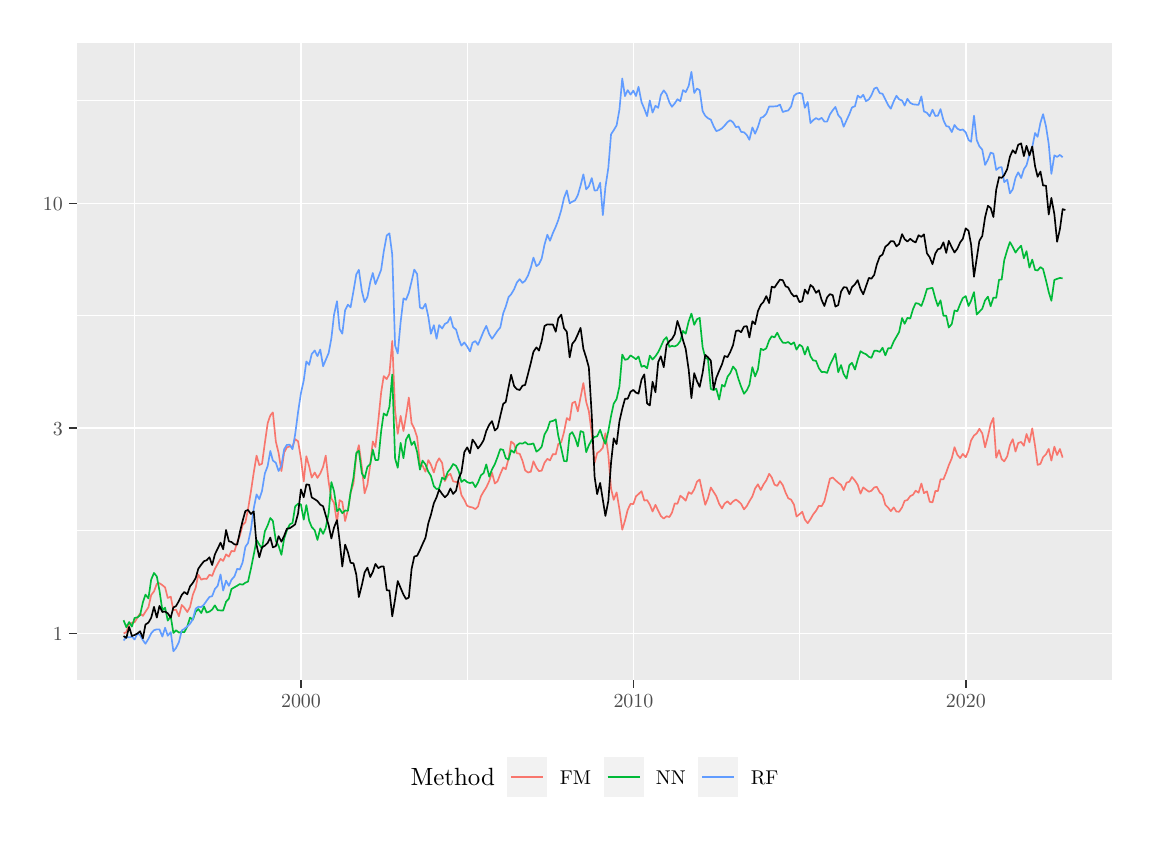
\begin{tikzpicture}[x=1pt,y=1pt]
\definecolor{fillColor}{RGB}{255,255,255}
\path[use as bounding box,fill=fillColor,fill opacity=0.00] (0,0) rectangle (397.48,289.08);
\begin{scope}
\path[clip] (  0.00,  0.00) rectangle (397.48,289.08);
\definecolor{drawColor}{RGB}{255,255,255}
\definecolor{fillColor}{RGB}{255,255,255}

\path[draw=drawColor,line width= 0.6pt,line join=round,line cap=round,fill=fillColor] (  0.00,  0.00) rectangle (397.48,289.08);
\end{scope}
\begin{scope}
\path[clip] ( 17.65, 53.26) rectangle (391.98,283.58);
\definecolor{fillColor}{gray}{0.92}

\path[fill=fillColor] ( 17.65, 53.26) rectangle (391.98,283.58);
\definecolor{drawColor}{RGB}{255,255,255}

\path[draw=drawColor,line width= 0.3pt,line join=round] ( 17.65,107.26) --
	(391.98,107.26);

\path[draw=drawColor,line width= 0.3pt,line join=round] ( 17.65,184.97) --
	(391.98,184.97);

\path[draw=drawColor,line width= 0.3pt,line join=round] ( 17.65,262.68) --
	(391.98,262.68);

\path[draw=drawColor,line width= 0.3pt,line join=round] ( 38.69, 53.26) --
	( 38.69,283.58);

\path[draw=drawColor,line width= 0.3pt,line join=round] (158.83, 53.26) --
	(158.83,283.58);

\path[draw=drawColor,line width= 0.3pt,line join=round] (278.94, 53.26) --
	(278.94,283.58);

\path[draw=drawColor,line width= 0.6pt,line join=round] ( 17.65, 70.18) --
	(391.98, 70.18);

\path[draw=drawColor,line width= 0.6pt,line join=round] ( 17.65,144.33) --
	(391.98,144.33);

\path[draw=drawColor,line width= 0.6pt,line join=round] ( 17.65,225.60) --
	(391.98,225.60);

\path[draw=drawColor,line width= 0.6pt,line join=round] ( 98.76, 53.26) --
	( 98.76,283.58);

\path[draw=drawColor,line width= 0.6pt,line join=round] (218.89, 53.26) --
	(218.89,283.58);

\path[draw=drawColor,line width= 0.6pt,line join=round] (338.99, 53.26) --
	(338.99,283.58);
\definecolor{drawColor}{RGB}{248,118,109}

\path[draw=drawColor,line width= 0.6pt,line join=round] ( 34.66, 70.20) --
	( 35.65, 70.67) --
	( 36.67, 73.56) --
	( 37.66, 74.05) --
	( 38.64, 74.23) --
	( 39.70, 76.01) --
	( 40.62, 77.38) --
	( 41.64, 76.54) --
	( 42.56, 78.02) --
	( 43.64, 79.62) --
	( 44.63, 84.06) --
	( 45.65, 85.38) --
	( 46.67, 88.13) --
	( 47.62, 88.35) --
	( 48.67, 87.64) --
	( 49.66, 86.81) --
	( 50.61, 83.00) --
	( 51.70, 83.46) --
	( 52.65, 78.63) --
	( 53.61, 78.74) --
	( 54.66, 76.40) --
	( 55.68, 80.48) --
	( 56.60, 79.51) --
	( 57.68, 77.92) --
	( 58.67, 79.72) --
	( 59.69, 84.18) --
	( 60.71, 86.72) --
	( 61.66, 91.44) --
	( 62.72, 89.60) --
	( 63.73, 90.00) --
	( 64.66, 89.87) --
	( 65.68, 91.38) --
	( 66.66, 90.97) --
	( 67.65, 93.49) --
	( 68.67, 95.36) --
	( 69.69, 97.13) --
	( 70.64, 96.39) --
	( 71.69, 98.75) --
	( 72.71, 97.95) --
	( 73.63, 99.99) --
	( 74.72, 99.84) --
	( 75.71,103.12) --
	( 76.63,105.34) --
	( 77.68,109.40) --
	( 78.67,110.35) --
	( 79.62,115.02) --
	( 80.67,121.48) --
	( 81.69,128.34) --
	( 82.71,134.44) --
	( 83.70,131.05) --
	( 84.68,131.51) --
	( 85.70,138.97) --
	( 86.72,146.10) --
	( 87.68,148.97) --
	( 88.60,150.05) --
	( 89.68,139.48) --
	( 90.67,135.42) --
	( 91.69,128.86) --
	( 92.67,135.54) --
	( 93.66,137.41) --
	( 94.71,137.78) --
	( 95.70,137.66) --
	( 96.65,140.38) --
	( 97.71,139.61) --
	( 98.73,133.53) --
	( 99.75,125.13) --
	(100.70,134.20) --
	(101.72,130.55) --
	(102.64,126.50) --
	(103.72,128.33) --
	(104.71,126.38) --
	(105.73,128.00) --
	(106.75,130.40) --
	(107.70,134.44) --
	(108.76,124.91) --
	(109.74,118.98) --
	(110.70,117.34) --
	(111.78,110.25) --
	(112.70,118.34) --
	(113.69,117.70) --
	(114.71,110.81) --
	(115.73,114.90) --
	(116.68,121.00) --
	(117.73,124.42) --
	(118.75,134.49) --
	(119.67,138.24) --
	(120.76,130.22) --
	(121.75,120.82) --
	(122.77,123.95) --
	(123.79,131.22) --
	(124.71,139.58) --
	(125.66,137.55) --
	(126.71,147.21) --
	(127.73,157.29) --
	(128.65,163.17) --
	(129.74,162.09) --
	(130.72,163.98) --
	(131.74,175.89) --
	(132.76,150.82) --
	(133.72,142.30) --
	(134.77,148.80) --
	(135.79,143.33) --
	(136.71,148.71) --
	(137.73,155.44) --
	(138.72,146.16) --
	(139.70,144.25) --
	(140.72,141.16) --
	(141.74,131.62) --
	(142.69,130.80) --
	(143.75,128.63) --
	(144.77,132.82) --
	(145.69,131.21) --
	(146.77,128.34) --
	(147.76,131.84) --
	(148.68,133.48) --
	(149.77,131.78) --
	(150.75,125.25) --
	(151.77,127.26) --
	(152.76,127.84) --
	(153.74,125.15) --
	(154.80,124.93) --
	(155.78,124.77) --
	(156.74,120.14) --
	(157.79,118.42) --
	(158.81,116.30) --
	(159.83,115.88) --
	(160.75,115.70) --
	(161.77,115.12) --
	(162.72,116.03) --
	(163.77,119.71) --
	(164.76,121.45) --
	(165.71,122.94) --
	(166.80,125.27) --
	(167.79,128.25) --
	(168.81,124.36) --
	(169.79,125.17) --
	(170.78,127.77) --
	(171.83,130.18) --
	(172.75,129.52) --
	(173.77,133.36) --
	(174.69,139.55) --
	(175.78,138.59) --
	(176.76,135.30) --
	(177.78,135.13) --
	(178.80,132.57) --
	(179.76,129.12) --
	(180.81,128.33) --
	(181.80,128.62) --
	(182.75,132.40) --
	(183.84,130.05) --
	(184.76,128.84) --
	(185.74,129.01) --
	(186.76,131.88) --
	(187.78,133.27) --
	(188.74,132.71) --
	(189.79,135.00) --
	(190.81,134.88) --
	(191.73,138.63) --
	(192.81,139.29) --
	(193.80,142.92) --
	(194.82,148.02) --
	(195.84,147.20) --
	(196.79,153.40) --
	(197.81,153.95) --
	(198.80,150.41) --
	(199.79,155.55) --
	(200.80,160.67) --
	(201.82,153.85) --
	(202.78,150.48) --
	(203.83,142.43) --
	(204.85,131.83) --
	(205.77,135.33) --
	(206.86,136.15) --
	(207.84,137.30) --
	(208.76,142.51) --
	(209.82,134.67) --
	(210.80,122.56) --
	(211.76,118.47) --
	(212.81,121.17) --
	(213.83,115.09) --
	(214.85,107.68) --
	(215.83,110.91) --
	(216.82,114.85) --
	(217.84,117.02) --
	(218.86,116.95) --
	(219.81,119.73) --
	(220.73,120.55) --
	(221.82,121.57) --
	(222.81,118.20) --
	(223.82,118.37) --
	(224.81,116.71) --
	(225.80,114.25) --
	(226.85,116.65) --
	(227.84,114.53) --
	(228.79,112.63) --
	(229.84,111.68) --
	(230.86,112.54) --
	(231.88,112.25) --
	(232.80,113.79) --
	(233.82,117.15) --
	(234.78,117.04) --
	(235.83,119.96) --
	(236.81,119.17) --
	(237.77,118.15) --
	(238.85,121.23) --
	(239.84,120.60) --
	(240.86,122.27) --
	(241.85,125.04) --
	(242.83,125.80) --
	(243.89,120.84) --
	(244.84,116.68) --
	(245.83,119.07) --
	(246.85,122.92) --
	(247.86,121.32) --
	(248.82,119.81) --
	(249.87,117.01) --
	(250.89,115.35) --
	(251.81,117.09) --
	(252.90,117.94) --
	(253.88,116.83) --
	(254.90,117.89) --
	(255.92,118.58) --
	(256.84,117.91) --
	(257.80,117.03) --
	(258.85,115.01) --
	(259.87,116.26) --
	(260.79,117.94) --
	(261.87,119.72) --
	(262.86,122.56) --
	(263.88,124.07) --
	(264.90,122.04) --
	(265.85,123.96) --
	(266.91,125.51) --
	(267.93,127.87) --
	(268.85,126.60) --
	(269.87,123.96) --
	(270.85,123.49) --
	(271.84,125.22) --
	(272.86,123.76) --
	(273.88,121.05) --
	(274.83,119.06) --
	(275.88,118.50) --
	(276.90,116.71) --
	(277.82,112.44) --
	(278.91,113.27) --
	(279.90,114.14) --
	(280.82,111.33) --
	(281.87,110.03) --
	(282.86,111.48) --
	(283.81,113.16) --
	(284.86,114.48) --
	(285.88,116.31) --
	(286.90,116.16) --
	(287.89,117.94) --
	(288.87,121.93) --
	(289.89,126.11) --
	(290.91,126.53) --
	(291.87,125.57) --
	(292.89,124.65) --
	(293.91,123.88) --
	(294.86,121.99) --
	(295.91,124.69) --
	(296.90,124.99) --
	(297.85,126.70) --
	(298.94,125.40) --
	(299.92,123.89) --
	(300.94,120.69) --
	(301.93,122.96) --
	(302.92,122.17) --
	(303.97,121.39) --
	(304.89,121.75) --
	(305.91,122.94) --
	(306.83,123.16) --
	(307.91,121.13) --
	(308.90,120.22) --
	(309.92,116.62) --
	(310.94,115.63) --
	(311.89,114.38) --
	(312.95,115.73) --
	(313.93,114.21) --
	(314.89,114.17) --
	(315.97,115.78) --
	(316.89,118.10) --
	(317.88,118.39) --
	(318.90,119.79) --
	(319.92,120.31) --
	(320.87,121.77) --
	(321.92,121.03) --
	(322.94,124.35) --
	(323.86,120.87) --
	(324.95,121.55) --
	(325.94,117.78) --
	(326.96,117.53) --
	(327.98,121.64) --
	(328.90,121.64) --
	(329.85,125.88) --
	(330.90,125.86) --
	(331.92,128.37) --
	(332.84,130.97) --
	(333.93,133.50) --
	(334.91,137.50) --
	(335.93,134.74) --
	(336.95,133.56) --
	(337.91,135.04) --
	(338.96,133.85) --
	(339.98,136.25) --
	(340.90,139.93) --
	(341.95,141.70) --
	(342.94,142.49) --
	(343.89,144.12) --
	(344.94,142.48) --
	(345.96,137.46) --
	(346.98,141.44) --
	(347.97,145.82) --
	(348.96,148.05) --
	(349.98,133.67) --
	(351.00,136.41) --
	(351.95,133.18) --
	(352.87,132.35) --
	(353.96,134.19) --
	(354.94,138.27) --
	(355.96,140.37) --
	(356.95,135.90) --
	(357.93,138.99) --
	(358.99,139.38) --
	(359.97,137.99) --
	(360.93,142.26) --
	(361.98,139.23) --
	(363.00,144.29) --
	(364.02,137.96) --
	(364.94,131.08) --
	(365.96,131.46) --
	(366.91,133.87) --
	(367.96,134.91) --
	(368.95,136.86) --
	(369.91,132.63) --
	(370.99,137.67) --
	(371.98,134.66) --
	(373.00,136.83) --
	(373.98,133.73);
\definecolor{drawColor}{RGB}{0,186,56}

\path[draw=drawColor,line width= 0.6pt,line join=round] ( 34.66, 74.95) --
	( 35.65, 72.44) --
	( 36.67, 74.31) --
	( 37.66, 72.67) --
	( 38.64, 75.80) --
	( 39.70, 75.99) --
	( 40.62, 76.80) --
	( 41.64, 81.48) --
	( 42.56, 84.22) --
	( 43.64, 82.86) --
	( 44.63, 89.66) --
	( 45.65, 92.04) --
	( 46.67, 90.76) --
	( 47.62, 85.67) --
	( 48.67, 78.58) --
	( 49.66, 79.52) --
	( 50.61, 74.82) --
	( 51.70, 76.34) --
	( 52.65, 70.35) --
	( 53.61, 71.32) --
	( 54.66, 70.51) --
	( 55.68, 70.73) --
	( 56.60, 70.62) --
	( 57.68, 72.71) --
	( 58.67, 75.91) --
	( 59.69, 75.15) --
	( 60.71, 78.02) --
	( 61.66, 79.00) --
	( 62.72, 77.57) --
	( 63.73, 79.93) --
	( 64.66, 77.73) --
	( 65.68, 78.06) --
	( 66.66, 78.81) --
	( 67.65, 80.33) --
	( 68.67, 78.58) --
	( 69.69, 78.50) --
	( 70.64, 78.45) --
	( 71.69, 81.67) --
	( 72.71, 82.75) --
	( 73.63, 86.21) --
	( 74.72, 86.86) --
	( 75.71, 87.42) --
	( 76.63, 88.03) --
	( 77.68, 87.81) --
	( 78.67, 88.53) --
	( 79.62, 88.90) --
	( 80.67, 93.59) --
	( 81.69, 98.62) --
	( 82.71,104.00) --
	( 83.70,102.33) --
	( 84.68,100.86) --
	( 85.70,107.05) --
	( 86.72,109.24) --
	( 87.68,111.90) --
	( 88.60,110.88) --
	( 89.68,103.68) --
	( 90.67,101.85) --
	( 91.69, 98.58) --
	( 92.67,104.46) --
	( 93.66,107.42) --
	( 94.71,109.59) --
	( 95.70,110.09) --
	( 96.65,116.06) --
	( 97.71,117.09) --
	( 98.73,116.83) --
	( 99.75,111.31) --
	(100.70,116.58) --
	(101.72,110.89) --
	(102.64,108.63) --
	(103.72,107.48) --
	(104.71,103.97) --
	(105.73,108.16) --
	(106.75,106.17) --
	(107.70,108.34) --
	(108.76,113.67) --
	(109.74,124.88) --
	(110.70,121.62) --
	(111.78,114.38) --
	(112.70,115.25) --
	(113.69,113.63) --
	(114.71,114.60) --
	(115.73,114.52) --
	(116.68,121.11) --
	(117.73,126.52) --
	(118.75,135.37) --
	(119.67,136.25) --
	(120.76,128.03) --
	(121.75,126.28) --
	(122.77,130.41) --
	(123.79,131.44) --
	(124.71,136.60) --
	(125.66,132.82) --
	(126.71,132.90) --
	(127.73,143.29) --
	(128.65,149.67) --
	(129.74,148.88) --
	(130.72,152.06) --
	(131.74,163.73) --
	(132.76,133.45) --
	(133.72,130.04) --
	(134.77,139.03) --
	(135.79,133.52) --
	(136.71,140.19) --
	(137.73,142.08) --
	(138.72,138.29) --
	(139.70,139.53) --
	(140.72,135.76) --
	(141.74,129.38) --
	(142.69,132.62) --
	(143.75,131.24) --
	(144.77,128.60) --
	(145.69,127.18) --
	(146.77,123.39) --
	(147.76,122.35) --
	(148.68,122.64) --
	(149.77,126.52) --
	(150.75,125.79) --
	(151.77,128.46) --
	(152.76,129.71) --
	(153.74,131.40) --
	(154.80,130.75) --
	(155.78,128.71) --
	(156.74,124.92) --
	(157.79,125.75) --
	(158.81,124.87) --
	(159.83,124.51) --
	(160.75,124.83) --
	(161.77,123.05) --
	(162.72,124.68) --
	(163.77,127.32) --
	(164.76,128.12) --
	(165.71,131.26) --
	(166.80,126.81) --
	(167.79,129.48) --
	(168.81,131.37) --
	(169.79,133.94) --
	(170.78,136.81) --
	(171.83,136.48) --
	(172.75,133.52) --
	(173.77,132.99) --
	(174.69,136.39) --
	(175.78,135.49) --
	(176.76,138.12) --
	(177.78,138.91) --
	(178.80,138.76) --
	(179.76,139.32) --
	(180.81,138.49) --
	(181.80,138.58) --
	(182.75,138.85) --
	(183.84,135.87) --
	(184.76,136.53) --
	(185.74,137.63) --
	(186.76,142.08) --
	(187.78,143.83) --
	(188.74,146.74) --
	(189.79,146.97) --
	(190.81,147.52) --
	(191.73,141.64) --
	(192.81,137.02) --
	(193.80,132.48) --
	(194.82,132.41) --
	(195.84,142.11) --
	(196.79,142.92) --
	(197.81,140.77) --
	(198.80,137.75) --
	(199.79,143.31) --
	(200.80,142.89) --
	(201.82,135.67) --
	(202.78,138.18) --
	(203.83,140.15) --
	(204.85,141.20) --
	(205.77,141.42) --
	(206.86,143.76) --
	(207.84,140.85) --
	(208.76,138.69) --
	(209.82,143.33) --
	(210.80,148.74) --
	(211.76,153.21) --
	(212.81,154.89) --
	(213.83,159.44) --
	(214.85,170.94) --
	(215.83,169.07) --
	(216.82,169.31) --
	(217.84,170.66) --
	(218.86,169.98) --
	(219.81,169.25) --
	(220.73,170.25) --
	(221.82,166.56) --
	(222.81,166.92) --
	(223.82,165.98) --
	(224.81,170.57) --
	(225.80,169.18) --
	(226.85,170.35) --
	(227.84,171.84) --
	(228.79,173.82) --
	(229.84,176.19) --
	(230.86,177.27) --
	(231.88,173.73) --
	(232.80,174.08) --
	(233.82,173.89) --
	(234.78,174.43) --
	(235.83,175.85) --
	(236.81,179.49) --
	(237.77,178.48) --
	(238.85,182.95) --
	(239.84,185.76) --
	(240.86,181.71) --
	(241.85,183.71) --
	(242.83,184.22) --
	(243.89,173.59) --
	(244.84,169.84) --
	(245.83,169.27) --
	(246.85,158.52) --
	(247.86,158.10) --
	(248.82,158.65) --
	(249.87,154.69) --
	(250.89,159.97) --
	(251.81,159.39) --
	(252.90,162.96) --
	(253.88,164.27) --
	(254.90,166.62) --
	(255.92,165.35) --
	(256.84,162.10) --
	(257.80,159.35) --
	(258.85,156.79) --
	(259.87,158.07) --
	(260.79,159.96) --
	(261.87,166.40) --
	(262.86,163.05) --
	(263.88,165.63) --
	(264.90,173.04) --
	(265.85,172.59) --
	(266.91,173.22) --
	(267.93,176.09) --
	(268.85,177.57) --
	(269.87,177.16) --
	(270.85,178.85) --
	(271.84,176.80) --
	(272.86,175.26) --
	(273.88,175.16) --
	(274.83,175.49) --
	(275.88,174.62) --
	(276.90,175.38) --
	(277.82,172.73) --
	(278.91,174.52) --
	(279.90,173.83) --
	(280.82,170.96) --
	(281.87,173.76) --
	(282.86,170.35) --
	(283.81,168.87) --
	(284.86,168.68) --
	(285.88,166.06) --
	(286.90,164.64) --
	(287.89,164.71) --
	(288.87,164.32) --
	(289.89,167.18) --
	(290.91,169.25) --
	(291.87,171.29) --
	(292.89,164.56) --
	(293.91,167.16) --
	(294.86,163.89) --
	(295.91,162.28) --
	(296.90,167.10) --
	(297.85,167.99) --
	(298.94,165.53) --
	(299.92,169.07) --
	(300.94,172.16) --
	(301.93,171.51) --
	(302.92,171.10) --
	(303.97,170.13) --
	(304.89,169.78) --
	(305.91,172.32) --
	(306.83,172.34) --
	(307.91,171.91) --
	(308.90,173.42) --
	(309.92,170.65) --
	(310.94,173.26) --
	(311.89,173.19) --
	(312.95,175.72) --
	(313.93,177.41) --
	(314.89,179.09) --
	(315.97,184.16) --
	(316.89,182.06) --
	(317.88,184.21) --
	(318.90,183.96) --
	(319.92,187.39) --
	(320.87,189.54) --
	(321.92,189.34) --
	(322.94,188.52) --
	(323.86,191.02) --
	(324.95,194.65) --
	(325.94,194.86) --
	(326.96,195.05) --
	(327.98,191.21) --
	(328.90,188.50) --
	(329.85,190.57) --
	(330.90,184.99) --
	(331.92,184.99) --
	(332.84,180.72) --
	(333.93,182.01) --
	(334.91,186.88) --
	(335.93,186.62) --
	(336.95,189.23) --
	(337.91,191.37) --
	(338.96,192.06) --
	(339.98,188.49) --
	(340.90,190.42) --
	(341.95,193.52) --
	(342.94,185.42) --
	(343.89,186.43) --
	(344.94,187.55) --
	(345.96,190.55) --
	(346.98,191.88) --
	(347.97,188.44) --
	(348.96,191.54) --
	(349.98,191.46) --
	(351.00,197.99) --
	(351.95,198.06) --
	(352.87,205.03) --
	(353.96,208.74) --
	(354.94,211.61) --
	(355.96,209.84) --
	(356.95,207.79) --
	(357.93,209.19) --
	(358.99,210.28) --
	(359.97,205.74) --
	(360.93,208.33) --
	(361.98,202.38) --
	(363.00,205.26) --
	(364.02,201.54) --
	(364.94,201.34) --
	(365.96,202.56) --
	(366.91,201.85) --
	(367.96,197.78) --
	(368.95,193.56) --
	(369.91,190.40) --
	(370.99,197.93) --
	(371.98,198.30) --
	(373.00,198.63) --
	(373.98,198.52);
\definecolor{drawColor}{RGB}{97,156,255}

\path[draw=drawColor,line width= 0.6pt,line join=round] ( 34.66, 67.63) --
	( 35.65, 68.90) --
	( 36.67, 68.76) --
	( 37.66, 69.01) --
	( 38.64, 68.01) --
	( 39.70, 70.19) --
	( 40.62, 69.53) --
	( 41.64, 67.76) --
	( 42.56, 66.47) --
	( 43.64, 68.24) --
	( 44.63, 70.23) --
	( 45.65, 71.35) --
	( 46.67, 71.67) --
	( 47.62, 71.65) --
	( 48.67, 69.03) --
	( 49.66, 72.24) --
	( 50.61, 69.35) --
	( 51.70, 70.67) --
	( 52.65, 63.73) --
	( 53.61, 64.92) --
	( 54.66, 67.08) --
	( 55.68, 71.28) --
	( 56.60, 71.83) --
	( 57.68, 72.74) --
	( 58.67, 73.68) --
	( 59.69, 75.33) --
	( 60.71, 79.14) --
	( 61.66, 79.82) --
	( 62.72, 79.71) --
	( 63.73, 80.64) --
	( 64.66, 82.00) --
	( 65.68, 83.37) --
	( 66.66, 83.67) --
	( 67.65, 86.24) --
	( 68.67, 87.41) --
	( 69.69, 91.50) --
	( 70.64, 85.69) --
	( 71.69, 89.28) --
	( 72.71, 87.37) --
	( 73.63, 89.57) --
	( 74.72, 90.79) --
	( 75.71, 93.54) --
	( 76.63, 93.28) --
	( 77.68, 95.90) --
	( 78.67,101.48) --
	( 79.62,102.85) --
	( 80.67,107.71) --
	( 81.69,115.34) --
	( 82.71,120.43) --
	( 83.70,118.70) --
	( 84.68,121.71) --
	( 85.70,127.98) --
	( 86.72,130.65) --
	( 87.68,136.13) --
	( 88.60,132.67) --
	( 89.68,131.86) --
	( 90.67,128.88) --
	( 91.69,130.77) --
	( 92.67,136.73) --
	( 93.66,138.33) --
	( 94.71,138.35) --
	( 95.70,136.74) --
	( 96.65,142.10) --
	( 97.71,150.20) --
	( 98.73,156.93) --
	( 99.75,161.56) --
	(100.70,168.47) --
	(101.72,167.24) --
	(102.64,171.14) --
	(103.72,172.42) --
	(104.71,170.40) --
	(105.73,172.77) --
	(106.75,166.73) --
	(107.70,169.01) --
	(108.76,171.51) --
	(109.74,176.82) --
	(110.70,185.36) --
	(111.78,190.24) --
	(112.70,180.23) --
	(113.69,178.49) --
	(114.71,187.01) --
	(115.73,188.99) --
	(116.68,188.05) --
	(117.73,193.91) --
	(118.75,199.93) --
	(119.67,201.58) --
	(120.76,193.89) --
	(121.75,189.92) --
	(122.77,191.76) --
	(123.79,197.14) --
	(124.71,200.43) --
	(125.66,196.39) --
	(126.71,198.96) --
	(127.73,201.62) --
	(128.65,208.08) --
	(129.74,213.98) --
	(130.72,214.78) --
	(131.74,207.03) --
	(132.76,174.23) --
	(133.72,171.35) --
	(134.77,182.72) --
	(135.79,191.26) --
	(136.71,190.76) --
	(137.73,193.29) --
	(138.72,197.40) --
	(139.70,201.65) --
	(140.72,200.08) --
	(141.74,187.99) --
	(142.69,187.52) --
	(143.75,189.31) --
	(144.77,184.67) --
	(145.69,178.46) --
	(146.77,181.57) --
	(147.76,176.68) --
	(148.68,181.60) --
	(149.77,180.37) --
	(150.75,182.03) --
	(151.77,182.59) --
	(152.76,184.53) --
	(153.74,180.84) --
	(154.80,179.99) --
	(155.78,176.56) --
	(156.74,174.18) --
	(157.79,175.34) --
	(158.81,173.85) --
	(159.83,172.08) --
	(160.75,175.23) --
	(161.77,175.83) --
	(162.72,174.46) --
	(163.77,176.98) --
	(164.76,179.40) --
	(165.71,181.33) --
	(166.80,178.31) --
	(167.79,176.68) --
	(168.81,178.08) --
	(169.79,179.57) --
	(170.78,180.75) --
	(171.83,185.87) --
	(172.75,188.27) --
	(173.77,191.72) --
	(174.69,192.73) --
	(175.78,194.57) --
	(176.76,196.97) --
	(177.78,198.19) --
	(178.80,196.85) --
	(179.76,197.63) --
	(180.81,199.54) --
	(181.80,202.34) --
	(182.75,206.00) --
	(183.84,202.90) --
	(184.76,203.62) --
	(185.74,205.68) --
	(186.76,210.68) --
	(187.78,214.26) --
	(188.74,212.08) --
	(189.79,214.88) --
	(190.81,217.13) --
	(191.73,219.55) --
	(192.81,223.19) --
	(193.80,227.54) --
	(194.82,230.25) --
	(195.84,225.61) --
	(196.79,226.20) --
	(197.81,226.68) --
	(198.80,228.58) --
	(199.79,232.04) --
	(200.80,236.08) --
	(201.82,230.65) --
	(202.78,231.72) --
	(203.83,234.72) --
	(204.85,230.23) --
	(205.77,230.31) --
	(206.86,233.02) --
	(207.84,221.34) --
	(208.76,231.41) --
	(209.82,238.45) --
	(210.80,250.54) --
	(211.76,252.02) --
	(212.81,253.76) --
	(213.83,259.45) --
	(214.85,270.69) --
	(215.83,264.36) --
	(216.82,266.52) --
	(217.84,264.88) --
	(218.86,266.34) --
	(219.81,264.38) --
	(220.73,267.73) --
	(221.82,262.15) --
	(222.81,259.81) --
	(223.82,257.12) --
	(224.81,262.76) --
	(225.80,258.39) --
	(226.85,260.85) --
	(227.84,260.12) --
	(228.79,264.75) --
	(229.84,266.42) --
	(230.86,265.05) --
	(231.88,262.04) --
	(232.80,260.49) --
	(233.82,261.72) --
	(234.78,263.22) --
	(235.83,262.52) --
	(236.81,266.52) --
	(237.77,265.79) --
	(238.85,268.01) --
	(239.84,273.11) --
	(240.86,265.47) --
	(241.85,267.07) --
	(242.83,266.49) --
	(243.89,258.93) --
	(244.84,257.22) --
	(245.83,256.34) --
	(246.85,255.85) --
	(247.86,253.47) --
	(248.82,251.69) --
	(249.87,252.08) --
	(250.89,252.70) --
	(251.81,253.67) --
	(252.90,254.97) --
	(253.88,255.65) --
	(254.90,254.84) --
	(255.92,253.12) --
	(256.84,253.37) --
	(257.80,251.43) --
	(258.85,251.27) --
	(259.87,250.23) --
	(260.79,248.60) --
	(261.87,253.03) --
	(262.86,250.77) --
	(263.88,253.18) --
	(264.90,256.49) --
	(265.85,256.87) --
	(266.91,258.00) --
	(267.93,260.59) --
	(268.85,260.57) --
	(269.87,260.64) --
	(270.85,260.73) --
	(271.84,261.30) --
	(272.86,258.60) --
	(273.88,258.94) --
	(274.83,259.16) --
	(275.88,260.61) --
	(276.90,264.44) --
	(277.82,265.22) --
	(278.91,265.50) --
	(279.90,265.18) --
	(280.82,260.13) --
	(281.87,262.24) --
	(282.86,254.61) --
	(283.81,255.63) --
	(284.86,256.39) --
	(285.88,255.85) --
	(286.90,256.50) --
	(287.89,255.14) --
	(288.87,255.14) --
	(289.89,257.73) --
	(290.91,259.25) --
	(291.87,260.44) --
	(292.89,257.50) --
	(293.91,256.29) --
	(294.86,253.28) --
	(295.91,255.65) --
	(296.90,257.79) --
	(297.85,260.25) --
	(298.94,260.69) --
	(299.92,264.53) --
	(300.94,263.72) --
	(301.93,264.82) --
	(302.92,262.50) --
	(303.97,263.17) --
	(304.89,264.67) --
	(305.91,267.08) --
	(306.83,267.46) --
	(307.91,265.40) --
	(308.90,265.21) --
	(309.92,263.10) --
	(310.94,261.06) --
	(311.89,259.80) --
	(312.95,262.49) --
	(313.93,264.47) --
	(314.89,263.17) --
	(315.97,262.77) --
	(316.89,260.92) --
	(317.88,263.37) --
	(318.90,261.91) --
	(319.92,261.39) --
	(320.87,261.28) --
	(321.92,261.18) --
	(322.94,264.23) --
	(323.86,258.81) --
	(324.95,258.30) --
	(325.94,257.05) --
	(326.96,259.43) --
	(327.98,257.17) --
	(328.90,257.26) --
	(329.85,259.66) --
	(330.90,255.66) --
	(331.92,253.50) --
	(332.84,253.31) --
	(333.93,251.35) --
	(334.91,253.91) --
	(335.93,252.59) --
	(336.95,252.05) --
	(337.91,252.29) --
	(338.96,251.26) --
	(339.98,248.51) --
	(340.90,247.84) --
	(341.95,257.27) --
	(342.94,248.47) --
	(343.89,246.23) --
	(344.94,244.99) --
	(345.96,239.48) --
	(346.98,241.36) --
	(347.97,243.93) --
	(348.96,243.54) --
	(349.98,237.65) --
	(351.00,238.54) --
	(351.95,238.67) --
	(352.87,233.25) --
	(353.96,234.19) --
	(354.94,229.20) --
	(355.96,230.69) --
	(356.95,234.81) --
	(357.93,236.81) --
	(358.99,234.73) --
	(359.97,237.90) --
	(360.93,239.36) --
	(361.98,243.25) --
	(363.00,245.87) --
	(364.02,251.03) --
	(364.94,249.61) --
	(365.96,254.72) --
	(366.91,257.82) --
	(367.96,253.48) --
	(368.95,247.08) --
	(369.91,236.24) --
	(370.99,242.93) --
	(371.98,242.37) --
	(373.00,243.10) --
	(373.98,242.27);
\definecolor{drawColor}{RGB}{0,0,0}

\path[draw=drawColor,line width= 0.6pt,line join=round] ( 34.66, 69.24) --
	( 35.65, 68.55) --
	( 36.67, 72.55) --
	( 37.66, 69.26) --
	( 38.64, 69.61) --
	( 39.70, 70.18) --
	( 40.62, 70.98) --
	( 41.64, 68.45) --
	( 42.56, 73.40) --
	( 43.64, 74.10) --
	( 44.63, 75.84) --
	( 45.65, 79.78) --
	( 46.67, 75.91) --
	( 47.62, 80.14) --
	( 48.67, 77.93) --
	( 49.66, 78.11) --
	( 50.61, 77.48) --
	( 51.70, 75.90) --
	( 52.65, 79.58) --
	( 53.61, 80.08) --
	( 54.66, 81.92) --
	( 55.68, 84.11) --
	( 56.60, 85.16) --
	( 57.68, 84.33) --
	( 58.67, 87.20) --
	( 59.69, 88.47) --
	( 60.71, 90.20) --
	( 61.66, 93.57) --
	( 62.72, 95.05) --
	( 63.73, 96.32) --
	( 64.66, 96.63) --
	( 65.68, 97.72) --
	( 66.66, 94.90) --
	( 67.65, 98.75) --
	( 68.67,100.84) --
	( 69.69,103.01) --
	( 70.64,100.61) --
	( 71.69,107.56) --
	( 72.71,103.45) --
	( 73.63,103.23) --
	( 74.72,102.37) --
	( 75.71,102.28) --
	( 76.63,106.58) --
	( 77.68,110.92) --
	( 78.67,114.44) --
	( 79.62,114.80) --
	( 80.67,113.34) --
	( 81.69,114.29) --
	( 82.71,102.14) --
	( 83.70, 97.71) --
	( 84.68,101.31) --
	( 85.70,101.90) --
	( 86.72,102.89) --
	( 87.68,104.83) --
	( 88.60,101.26) --
	( 89.68,101.76) --
	( 90.67,105.35) --
	( 91.69,103.34) --
	( 92.67,105.42) --
	( 93.66,108.00) --
	( 94.71,108.22) --
	( 95.70,108.88) --
	( 96.65,109.59) --
	( 97.71,113.53) --
	( 98.73,122.24) --
	( 99.75,119.38) --
	(100.70,124.04) --
	(101.72,123.87) --
	(102.64,119.34) --
	(103.72,118.69) --
	(104.71,118.03) --
	(105.73,116.72) --
	(106.75,116.15) --
	(107.70,112.86) --
	(108.76,109.27) --
	(109.74,104.49) --
	(110.70,108.48) --
	(111.78,111.14) --
	(112.70,103.67) --
	(113.69, 94.38) --
	(114.71,102.29) --
	(115.73, 99.51) --
	(116.68, 95.70) --
	(117.73, 95.54) --
	(118.75, 91.43) --
	(119.67, 83.34) --
	(120.76, 87.66) --
	(121.75, 92.23) --
	(122.77, 93.96) --
	(123.79, 90.58) --
	(124.71, 92.39) --
	(125.66, 95.32) --
	(126.71, 93.77) --
	(127.73, 94.37) --
	(128.65, 94.41) --
	(129.74, 85.80) --
	(130.72, 85.70) --
	(131.74, 76.36) --
	(132.76, 82.56) --
	(133.72, 89.12) --
	(134.77, 86.61) --
	(135.79, 84.22) --
	(136.71, 82.64) --
	(137.73, 83.16) --
	(138.72, 93.44) --
	(139.70, 97.97) --
	(140.72, 98.26) --
	(141.74,100.29) --
	(142.69,102.48) --
	(143.75,104.76) --
	(144.77,110.00) --
	(145.69,112.98) --
	(146.77,117.25) --
	(147.76,119.38) --
	(148.68,122.15) --
	(149.77,120.57) --
	(150.75,119.40) --
	(151.77,120.36) --
	(152.76,122.57) --
	(153.74,120.59) --
	(154.80,121.80) --
	(155.78,126.29) --
	(156.74,128.45) --
	(157.79,135.72) --
	(158.81,137.42) --
	(159.83,135.30) --
	(160.75,140.24) --
	(161.77,138.82) --
	(162.72,137.02) --
	(163.77,138.36) --
	(164.76,140.03) --
	(165.71,143.34) --
	(166.80,145.64) --
	(167.79,146.91) --
	(168.81,143.52) --
	(169.79,144.44) --
	(170.78,148.79) --
	(171.83,153.14) --
	(172.75,153.82) --
	(173.77,159.17) --
	(174.69,163.66) --
	(175.78,159.55) --
	(176.76,158.45) --
	(177.78,158.13) --
	(178.80,159.69) --
	(179.76,159.98) --
	(180.81,164.01) --
	(181.80,167.90) --
	(182.75,171.96) --
	(183.84,173.56) --
	(184.76,172.38) --
	(185.74,175.89) --
	(186.76,181.26) --
	(187.78,181.88) --
	(188.74,181.81) --
	(189.79,181.80) --
	(190.81,179.21) --
	(191.73,184.03) --
	(192.81,185.35) --
	(193.80,180.50) --
	(194.82,179.20) --
	(195.84,169.95) --
	(196.79,174.86) --
	(197.81,176.10) --
	(198.80,178.28) --
	(199.79,180.59) --
	(200.80,173.03) --
	(201.82,169.85) --
	(202.78,166.29) --
	(203.83,148.98) --
	(204.85,126.88) --
	(205.77,120.51) --
	(206.86,124.59) --
	(207.84,118.43) --
	(208.76,112.65) --
	(209.82,118.06) --
	(210.80,131.88) --
	(211.76,140.70) --
	(212.81,138.58) --
	(213.83,146.85) --
	(214.85,151.32) --
	(215.83,154.96) --
	(216.82,155.01) --
	(217.84,157.51) --
	(218.86,158.18) --
	(219.81,157.21) --
	(220.73,156.84) --
	(221.82,161.95) --
	(222.81,163.79) --
	(223.82,153.31) --
	(224.81,152.56) --
	(225.80,161.12) --
	(226.85,157.34) --
	(227.84,168.22) --
	(228.79,170.32) --
	(229.84,166.40) --
	(230.86,174.40) --
	(231.88,175.80) --
	(232.80,176.56) --
	(233.82,178.32) --
	(234.78,183.10) --
	(235.83,179.89) --
	(236.81,176.12) --
	(237.77,173.02) --
	(238.85,165.52) --
	(239.84,155.23) --
	(240.86,164.23) --
	(241.85,161.36) --
	(242.83,159.27) --
	(243.89,164.39) --
	(244.84,170.83) --
	(245.83,169.96) --
	(246.85,168.78) --
	(247.86,158.42) --
	(248.82,162.51) --
	(249.87,165.09) --
	(250.89,167.44) --
	(251.81,170.43) --
	(252.90,170.05) --
	(253.88,171.91) --
	(254.90,174.42) --
	(255.92,179.44) --
	(256.84,179.69) --
	(257.80,179.04) --
	(258.85,181.07) --
	(259.87,181.22) --
	(260.79,177.14) --
	(261.87,183.01) --
	(262.86,181.94) --
	(263.88,186.67) --
	(264.90,188.92) --
	(265.85,189.94) --
	(266.91,192.08) --
	(267.93,189.55) --
	(268.85,195.48) --
	(269.87,195.16) --
	(270.85,196.66) --
	(271.84,198.02) --
	(272.86,197.83) --
	(273.88,195.62) --
	(274.83,195.21) --
	(275.88,193.14) --
	(276.90,191.96) --
	(277.82,192.30) --
	(278.91,189.87) --
	(279.90,190.28) --
	(280.82,194.45) --
	(281.87,192.90) --
	(282.86,196.10) --
	(283.81,195.30) --
	(284.86,193.27) --
	(285.88,194.19) --
	(286.90,190.65) --
	(287.89,188.51) --
	(288.87,191.62) --
	(289.89,192.80) --
	(290.91,192.40) --
	(291.87,188.32) --
	(292.89,188.80) --
	(293.91,193.71) --
	(294.86,195.26) --
	(295.91,195.24) --
	(296.90,192.80) --
	(297.85,195.31) --
	(298.94,196.35) --
	(299.92,197.85) --
	(300.94,194.63) --
	(301.93,192.74) --
	(302.92,195.60) --
	(303.97,198.66) --
	(304.89,198.37) --
	(305.91,199.79) --
	(306.83,203.50) --
	(307.91,206.40) --
	(308.90,207.10) --
	(309.92,209.94) --
	(310.94,210.74) --
	(311.89,211.94) --
	(312.95,211.86) --
	(313.93,210.07) --
	(314.89,210.89) --
	(315.97,214.48) --
	(316.89,212.66) --
	(317.88,211.78) --
	(318.90,212.80) --
	(319.92,211.95) --
	(320.87,211.47) --
	(321.92,214.07) --
	(322.94,213.48) --
	(323.86,214.39) --
	(324.95,207.54) --
	(325.94,206.12) --
	(326.96,203.60) --
	(327.98,207.46) --
	(328.90,209.01) --
	(329.85,209.26) --
	(330.90,211.51) --
	(331.92,207.70) --
	(332.84,212.03) --
	(333.93,209.68) --
	(334.91,207.84) --
	(335.93,209.19) --
	(336.95,211.49) --
	(337.91,212.77) --
	(338.96,216.58) --
	(339.98,215.68) --
	(340.90,210.69) --
	(341.95,199.08) --
	(342.94,205.74) --
	(343.89,212.05) --
	(344.94,213.81) --
	(345.96,220.57) --
	(346.98,224.72) --
	(347.97,223.94) --
	(348.96,220.67) --
	(349.98,230.54) --
	(351.00,235.05) --
	(351.95,234.81) --
	(352.87,235.79) --
	(353.96,238.04) --
	(354.94,242.51) --
	(355.96,244.79) --
	(356.95,243.65) --
	(357.93,246.77) --
	(358.99,247.24) --
	(359.97,242.65) --
	(360.93,246.38) --
	(361.98,242.91) --
	(363.00,246.14) --
	(364.02,239.01) --
	(364.94,235.21) --
	(365.96,237.08) --
	(366.91,232.04) --
	(367.96,232.00) --
	(368.95,221.56) --
	(369.91,227.54) --
	(370.99,221.70) --
	(371.98,211.73) --
	(373.00,216.28) --
	(373.98,223.50) --
	(374.97,223.18);
\end{scope}
\begin{scope}
\path[clip] (  0.00,  0.00) rectangle (397.48,289.08);
\definecolor{drawColor}{gray}{0.30}

\node[text=drawColor,anchor=base east,inner sep=0pt, outer sep=0pt, scale=  0.72] at ( 12.70, 67.70) {1};

\node[text=drawColor,anchor=base east,inner sep=0pt, outer sep=0pt, scale=  0.72] at ( 12.70,141.86) {3};

\node[text=drawColor,anchor=base east,inner sep=0pt, outer sep=0pt, scale=  0.72] at ( 12.70,223.12) {10};
\end{scope}
\begin{scope}
\path[clip] (  0.00,  0.00) rectangle (397.48,289.08);
\definecolor{drawColor}{gray}{0.20}

\path[draw=drawColor,line width= 0.6pt,line join=round] ( 14.90, 70.18) --
	( 17.65, 70.18);

\path[draw=drawColor,line width= 0.6pt,line join=round] ( 14.90,144.33) --
	( 17.65,144.33);

\path[draw=drawColor,line width= 0.6pt,line join=round] ( 14.90,225.60) --
	( 17.65,225.60);
\end{scope}
\begin{scope}
\path[clip] (  0.00,  0.00) rectangle (397.48,289.08);
\definecolor{drawColor}{gray}{0.20}

\path[draw=drawColor,line width= 0.6pt,line join=round] ( 98.76, 50.51) --
	( 98.76, 53.26);

\path[draw=drawColor,line width= 0.6pt,line join=round] (218.89, 50.51) --
	(218.89, 53.26);

\path[draw=drawColor,line width= 0.6pt,line join=round] (338.99, 50.51) --
	(338.99, 53.26);
\end{scope}
\begin{scope}
\path[clip] (  0.00,  0.00) rectangle (397.48,289.08);
\definecolor{drawColor}{gray}{0.30}

\node[text=drawColor,anchor=base,inner sep=0pt, outer sep=0pt, scale=  0.72] at ( 98.76, 43.35) {2000};

\node[text=drawColor,anchor=base,inner sep=0pt, outer sep=0pt, scale=  0.72] at (218.89, 43.35) {2010};

\node[text=drawColor,anchor=base,inner sep=0pt, outer sep=0pt, scale=  0.72] at (338.99, 43.35) {2020};
\end{scope}
\begin{scope}
\path[clip] (  0.00,  0.00) rectangle (397.48,289.08);
\definecolor{fillColor}{RGB}{255,255,255}

\path[fill=fillColor] (132.84,  5.50) rectangle (276.79, 30.95);
\end{scope}
\begin{scope}
\path[clip] (  0.00,  0.00) rectangle (397.48,289.08);
\definecolor{drawColor}{RGB}{0,0,0}

\node[text=drawColor,anchor=base west,inner sep=0pt, outer sep=0pt, scale=  0.90] at (138.34, 15.13) {Method};
\end{scope}
\begin{scope}
\path[clip] (  0.00,  0.00) rectangle (397.48,289.08);
\definecolor{fillColor}{gray}{0.95}

\path[fill=fillColor] (173.34, 11.00) rectangle (187.79, 25.45);
\end{scope}
\begin{scope}
\path[clip] (  0.00,  0.00) rectangle (397.48,289.08);
\definecolor{drawColor}{RGB}{248,118,109}

\path[draw=drawColor,line width= 0.6pt,line join=round] (174.78, 18.23) -- (186.34, 18.23);
\end{scope}
\begin{scope}
\path[clip] (  0.00,  0.00) rectangle (397.48,289.08);
\definecolor{fillColor}{gray}{0.95}

\path[fill=fillColor] (208.09, 11.00) rectangle (222.54, 25.45);
\end{scope}
\begin{scope}
\path[clip] (  0.00,  0.00) rectangle (397.48,289.08);
\definecolor{drawColor}{RGB}{0,186,56}

\path[draw=drawColor,line width= 0.6pt,line join=round] (209.53, 18.23) -- (221.10, 18.23);
\end{scope}
\begin{scope}
\path[clip] (  0.00,  0.00) rectangle (397.48,289.08);
\definecolor{fillColor}{gray}{0.95}

\path[fill=fillColor] (242.34, 11.00) rectangle (256.79, 25.45);
\end{scope}
\begin{scope}
\path[clip] (  0.00,  0.00) rectangle (397.48,289.08);
\definecolor{drawColor}{RGB}{97,156,255}

\path[draw=drawColor,line width= 0.6pt,line join=round] (243.78, 18.23) -- (255.35, 18.23);
\end{scope}
\begin{scope}
\path[clip] (  0.00,  0.00) rectangle (397.48,289.08);
\definecolor{drawColor}{RGB}{0,0,0}

\node[text=drawColor,anchor=base west,inner sep=0pt, outer sep=0pt, scale=  0.72] at (192.29, 15.75) {FM};
\end{scope}
\begin{scope}
\path[clip] (  0.00,  0.00) rectangle (397.48,289.08);
\definecolor{drawColor}{RGB}{0,0,0}

\node[text=drawColor,anchor=base west,inner sep=0pt, outer sep=0pt, scale=  0.72] at (227.04, 15.75) {NN};
\end{scope}
\begin{scope}
\path[clip] (  0.00,  0.00) rectangle (397.48,289.08);
\definecolor{drawColor}{RGB}{0,0,0}

\node[text=drawColor,anchor=base west,inner sep=0pt, outer sep=0pt, scale=  0.72] at (261.29, 15.75) {RF};
\end{scope}
\end{tikzpicture}

\label{plot:cumul_vw_LS_portf_return}
\end{figure}

\subsection{Variable importance}\label{VariableImportance}

\begin{figure}[ht]
\centering
\caption[Variable importance]{\textbf{Variable importance}\\ Figure plots the importance of the explanatory variables to the predictive performance of the three machine learning models. Variable importance is defined as reduction in out-of-sample $R^2$ when corresponding variable is replaced by zero before the training process. Definition of the out-of-sample $R^2$ is described in section \ref{Methodology}. Darker colour indicates higher variable importance. FM stands for linear regression model, RF stand for random forest model and NN stands for neural networks model.}
% Created by tikzDevice version 0.12.6 on 2024-03-24 19:10:19
% !TEX encoding = UTF-8 Unicode
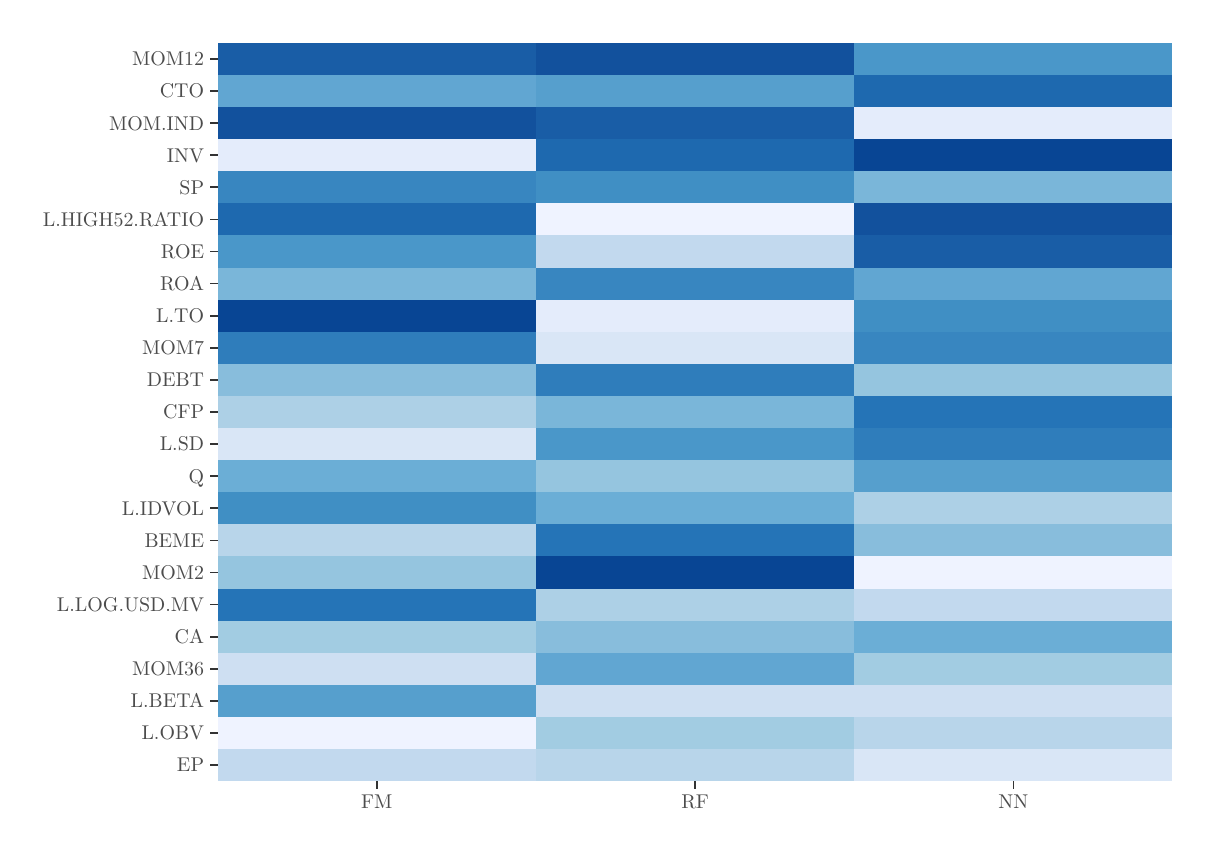
\begin{tikzpicture}[x=1pt,y=1pt]
\definecolor{fillColor}{RGB}{255,255,255}
\path[use as bounding box,fill=fillColor,fill opacity=0.00] (0,0) rectangle (419.17,289.08);
\begin{scope}
\path[clip] (  0.00,  0.00) rectangle (419.17,289.08);
\definecolor{drawColor}{RGB}{255,255,255}
\definecolor{fillColor}{RGB}{255,255,255}

\path[draw=drawColor,line width= 0.6pt,line join=round,line cap=round,fill=fillColor] (  0.00,  0.00) rectangle (419.17,289.08);
\end{scope}
\begin{scope}
\path[clip] ( 68.69, 16.81) rectangle (413.67,283.58);
\definecolor{fillColor}{gray}{0.92}

\path[fill=fillColor] ( 68.69, 16.81) rectangle (413.67,283.58);
\definecolor{drawColor}{RGB}{255,255,255}

\path[draw=drawColor,line width= 0.6pt,line join=round] ( 68.69, 22.61) --
	(413.67, 22.61);

\path[draw=drawColor,line width= 0.6pt,line join=round] ( 68.69, 34.21) --
	(413.67, 34.21);

\path[draw=drawColor,line width= 0.6pt,line join=round] ( 68.69, 45.81) --
	(413.67, 45.81);

\path[draw=drawColor,line width= 0.6pt,line join=round] ( 68.69, 57.40) --
	(413.67, 57.40);

\path[draw=drawColor,line width= 0.6pt,line join=round] ( 68.69, 69.00) --
	(413.67, 69.00);

\path[draw=drawColor,line width= 0.6pt,line join=round] ( 68.69, 80.60) --
	(413.67, 80.60);

\path[draw=drawColor,line width= 0.6pt,line join=round] ( 68.69, 92.20) --
	(413.67, 92.20);

\path[draw=drawColor,line width= 0.6pt,line join=round] ( 68.69,103.80) --
	(413.67,103.80);

\path[draw=drawColor,line width= 0.6pt,line join=round] ( 68.69,115.40) --
	(413.67,115.40);

\path[draw=drawColor,line width= 0.6pt,line join=round] ( 68.69,127.00) --
	(413.67,127.00);

\path[draw=drawColor,line width= 0.6pt,line join=round] ( 68.69,138.60) --
	(413.67,138.60);

\path[draw=drawColor,line width= 0.6pt,line join=round] ( 68.69,150.19) --
	(413.67,150.19);

\path[draw=drawColor,line width= 0.6pt,line join=round] ( 68.69,161.79) --
	(413.67,161.79);

\path[draw=drawColor,line width= 0.6pt,line join=round] ( 68.69,173.39) --
	(413.67,173.39);

\path[draw=drawColor,line width= 0.6pt,line join=round] ( 68.69,184.99) --
	(413.67,184.99);

\path[draw=drawColor,line width= 0.6pt,line join=round] ( 68.69,196.59) --
	(413.67,196.59);

\path[draw=drawColor,line width= 0.6pt,line join=round] ( 68.69,208.19) --
	(413.67,208.19);

\path[draw=drawColor,line width= 0.6pt,line join=round] ( 68.69,219.79) --
	(413.67,219.79);

\path[draw=drawColor,line width= 0.6pt,line join=round] ( 68.69,231.39) --
	(413.67,231.39);

\path[draw=drawColor,line width= 0.6pt,line join=round] ( 68.69,242.98) --
	(413.67,242.98);

\path[draw=drawColor,line width= 0.6pt,line join=round] ( 68.69,254.58) --
	(413.67,254.58);

\path[draw=drawColor,line width= 0.6pt,line join=round] ( 68.69,266.18) --
	(413.67,266.18);

\path[draw=drawColor,line width= 0.6pt,line join=round] ( 68.69,277.78) --
	(413.67,277.78);

\path[draw=drawColor,line width= 0.6pt,line join=round] (126.18, 16.81) --
	(126.18,283.58);

\path[draw=drawColor,line width= 0.6pt,line join=round] (241.18, 16.81) --
	(241.18,283.58);

\path[draw=drawColor,line width= 0.6pt,line join=round] (356.17, 16.81) --
	(356.17,283.58);
\definecolor{fillColor}{RGB}{37,116,183}

\path[fill=fillColor] (183.68, 98.00) rectangle (298.67,109.60);
\definecolor{fillColor}{RGB}{136,189,220}

\path[fill=fillColor] (183.68, 63.20) rectangle (298.67, 74.80);
\definecolor{fillColor}{RGB}{122,182,217}

\path[fill=fillColor] (183.68,144.39) rectangle (298.67,155.99);
\definecolor{fillColor}{RGB}{86,159,205}

\path[fill=fillColor] (183.68,260.38) rectangle (298.67,271.98);
\definecolor{fillColor}{RGB}{47,125,187}

\path[fill=fillColor] (183.68,155.99) rectangle (298.67,167.59);
\definecolor{fillColor}{RGB}{184,213,234}

\path[fill=fillColor] (183.68, 16.81) rectangle (298.67, 28.41);
\definecolor{fillColor}{RGB}{30,105,175}

\path[fill=fillColor] (183.68,237.18) rectangle (298.67,248.78);
\definecolor{fillColor}{RGB}{206,223,242}

\path[fill=fillColor] (183.68, 40.01) rectangle (298.67, 51.60);
\definecolor{fillColor}{RGB}{239,243,255}

\path[fill=fillColor] (183.68,213.99) rectangle (298.67,225.59);
\definecolor{fillColor}{RGB}{107,174,214}

\path[fill=fillColor] (183.68,109.60) rectangle (298.67,121.20);
\definecolor{fillColor}{RGB}{173,208,230}

\path[fill=fillColor] (183.68, 74.80) rectangle (298.67, 86.40);
\definecolor{fillColor}{RGB}{162,204,226}

\path[fill=fillColor] (183.68, 28.41) rectangle (298.67, 40.01);
\definecolor{fillColor}{RGB}{74,151,201}

\path[fill=fillColor] (183.68,132.80) rectangle (298.67,144.39);
\definecolor{fillColor}{RGB}{228,236,251}

\path[fill=fillColor] (183.68,179.19) rectangle (298.67,190.79);
\definecolor{fillColor}{RGB}{25,93,166}

\path[fill=fillColor] (183.68,248.78) rectangle (298.67,260.38);
\definecolor{fillColor}{RGB}{18,81,157}

\path[fill=fillColor] (183.68,271.98) rectangle (298.67,283.58);
\definecolor{fillColor}{RGB}{8,69,148}

\path[fill=fillColor] (183.68, 86.40) rectangle (298.67, 98.00);
\definecolor{fillColor}{RGB}{97,166,210}

\path[fill=fillColor] (183.68, 51.60) rectangle (298.67, 63.20);
\definecolor{fillColor}{RGB}{217,230,246}

\path[fill=fillColor] (183.68,167.59) rectangle (298.67,179.19);
\definecolor{fillColor}{RGB}{149,197,223}

\path[fill=fillColor] (183.68,121.20) rectangle (298.67,132.80);
\definecolor{fillColor}{RGB}{56,134,192}

\path[fill=fillColor] (183.68,190.79) rectangle (298.67,202.39);
\definecolor{fillColor}{RGB}{194,217,238}

\path[fill=fillColor] (183.68,202.39) rectangle (298.67,213.99);
\definecolor{fillColor}{RGB}{64,143,196}

\path[fill=fillColor] (183.68,225.59) rectangle (298.67,237.18);
\definecolor{fillColor}{RGB}{184,213,234}

\path[fill=fillColor] ( 68.69, 98.00) rectangle (183.68,109.60);
\definecolor{fillColor}{RGB}{162,204,226}

\path[fill=fillColor] ( 68.69, 63.20) rectangle (183.68, 74.80);
\definecolor{fillColor}{RGB}{173,208,230}

\path[fill=fillColor] ( 68.69,144.39) rectangle (183.68,155.99);
\definecolor{fillColor}{RGB}{97,166,210}

\path[fill=fillColor] ( 68.69,260.38) rectangle (183.68,271.98);
\definecolor{fillColor}{RGB}{136,189,220}

\path[fill=fillColor] ( 68.69,155.99) rectangle (183.68,167.59);
\definecolor{fillColor}{RGB}{194,217,238}

\path[fill=fillColor] ( 68.69, 16.81) rectangle (183.68, 28.41);
\definecolor{fillColor}{RGB}{228,236,251}

\path[fill=fillColor] ( 68.69,237.18) rectangle (183.68,248.78);
\definecolor{fillColor}{RGB}{86,159,205}

\path[fill=fillColor] ( 68.69, 40.01) rectangle (183.68, 51.60);
\definecolor{fillColor}{RGB}{30,105,175}

\path[fill=fillColor] ( 68.69,213.99) rectangle (183.68,225.59);
\definecolor{fillColor}{RGB}{64,143,196}

\path[fill=fillColor] ( 68.69,109.60) rectangle (183.68,121.20);
\definecolor{fillColor}{RGB}{37,116,183}

\path[fill=fillColor] ( 68.69, 74.80) rectangle (183.68, 86.40);
\definecolor{fillColor}{RGB}{239,243,255}

\path[fill=fillColor] ( 68.69, 28.41) rectangle (183.68, 40.01);
\definecolor{fillColor}{RGB}{217,230,246}

\path[fill=fillColor] ( 68.69,132.80) rectangle (183.68,144.39);
\definecolor{fillColor}{RGB}{8,69,148}

\path[fill=fillColor] ( 68.69,179.19) rectangle (183.68,190.79);
\definecolor{fillColor}{RGB}{18,81,157}

\path[fill=fillColor] ( 68.69,248.78) rectangle (183.68,260.38);
\definecolor{fillColor}{RGB}{25,93,166}

\path[fill=fillColor] ( 68.69,271.98) rectangle (183.68,283.58);
\definecolor{fillColor}{RGB}{149,197,223}

\path[fill=fillColor] ( 68.69, 86.40) rectangle (183.68, 98.00);
\definecolor{fillColor}{RGB}{206,223,242}

\path[fill=fillColor] ( 68.69, 51.60) rectangle (183.68, 63.20);
\definecolor{fillColor}{RGB}{47,125,187}

\path[fill=fillColor] ( 68.69,167.59) rectangle (183.68,179.19);
\definecolor{fillColor}{RGB}{107,174,214}

\path[fill=fillColor] ( 68.69,121.20) rectangle (183.68,132.80);
\definecolor{fillColor}{RGB}{122,182,217}

\path[fill=fillColor] ( 68.69,190.79) rectangle (183.68,202.39);
\definecolor{fillColor}{RGB}{74,151,201}

\path[fill=fillColor] ( 68.69,202.39) rectangle (183.68,213.99);
\definecolor{fillColor}{RGB}{56,134,192}

\path[fill=fillColor] ( 68.69,225.59) rectangle (183.68,237.18);
\definecolor{fillColor}{RGB}{136,189,220}

\path[fill=fillColor] (298.67, 98.00) rectangle (413.67,109.60);
\definecolor{fillColor}{RGB}{107,174,214}

\path[fill=fillColor] (298.67, 63.20) rectangle (413.67, 74.80);
\definecolor{fillColor}{RGB}{37,116,183}

\path[fill=fillColor] (298.67,144.39) rectangle (413.67,155.99);
\definecolor{fillColor}{RGB}{30,105,175}

\path[fill=fillColor] (298.67,260.38) rectangle (413.67,271.98);
\definecolor{fillColor}{RGB}{149,197,223}

\path[fill=fillColor] (298.67,155.99) rectangle (413.67,167.59);
\definecolor{fillColor}{RGB}{217,230,246}

\path[fill=fillColor] (298.67, 16.81) rectangle (413.67, 28.41);
\definecolor{fillColor}{RGB}{8,69,148}

\path[fill=fillColor] (298.67,237.18) rectangle (413.67,248.78);
\definecolor{fillColor}{RGB}{206,223,242}

\path[fill=fillColor] (298.67, 40.01) rectangle (413.67, 51.60);
\definecolor{fillColor}{RGB}{18,81,157}

\path[fill=fillColor] (298.67,213.99) rectangle (413.67,225.59);
\definecolor{fillColor}{RGB}{173,208,230}

\path[fill=fillColor] (298.67,109.60) rectangle (413.67,121.20);
\definecolor{fillColor}{RGB}{194,217,238}

\path[fill=fillColor] (298.67, 74.80) rectangle (413.67, 86.40);
\definecolor{fillColor}{RGB}{184,213,234}

\path[fill=fillColor] (298.67, 28.41) rectangle (413.67, 40.01);
\definecolor{fillColor}{RGB}{47,125,187}

\path[fill=fillColor] (298.67,132.80) rectangle (413.67,144.39);
\definecolor{fillColor}{RGB}{64,143,196}

\path[fill=fillColor] (298.67,179.19) rectangle (413.67,190.79);
\definecolor{fillColor}{RGB}{228,236,251}

\path[fill=fillColor] (298.67,248.78) rectangle (413.67,260.38);
\definecolor{fillColor}{RGB}{74,151,201}

\path[fill=fillColor] (298.67,271.98) rectangle (413.67,283.58);
\definecolor{fillColor}{RGB}{239,243,255}

\path[fill=fillColor] (298.67, 86.40) rectangle (413.67, 98.00);
\definecolor{fillColor}{RGB}{162,204,226}

\path[fill=fillColor] (298.67, 51.60) rectangle (413.67, 63.20);
\definecolor{fillColor}{RGB}{56,134,192}

\path[fill=fillColor] (298.67,167.59) rectangle (413.67,179.19);
\definecolor{fillColor}{RGB}{86,159,205}

\path[fill=fillColor] (298.67,121.20) rectangle (413.67,132.80);
\definecolor{fillColor}{RGB}{97,166,210}

\path[fill=fillColor] (298.67,190.79) rectangle (413.67,202.39);
\definecolor{fillColor}{RGB}{25,93,166}

\path[fill=fillColor] (298.67,202.39) rectangle (413.67,213.99);
\definecolor{fillColor}{RGB}{122,182,217}

\path[fill=fillColor] (298.67,225.59) rectangle (413.67,237.18);
\end{scope}
\begin{scope}
\path[clip] (  0.00,  0.00) rectangle (419.17,289.08);
\definecolor{drawColor}{gray}{0.30}

\node[text=drawColor,anchor=base east,inner sep=0pt, outer sep=0pt, scale=  0.72] at ( 63.74, 20.13) {EP};

\node[text=drawColor,anchor=base east,inner sep=0pt, outer sep=0pt, scale=  0.72] at ( 63.74, 31.73) {L.OBV};

\node[text=drawColor,anchor=base east,inner sep=0pt, outer sep=0pt, scale=  0.72] at ( 63.74, 43.33) {L.BETA};

\node[text=drawColor,anchor=base east,inner sep=0pt, outer sep=0pt, scale=  0.72] at ( 63.74, 54.92) {MOM36};

\node[text=drawColor,anchor=base east,inner sep=0pt, outer sep=0pt, scale=  0.72] at ( 63.74, 66.52) {CA};

\node[text=drawColor,anchor=base east,inner sep=0pt, outer sep=0pt, scale=  0.72] at ( 63.74, 78.12) {L.LOG.USD.MV};

\node[text=drawColor,anchor=base east,inner sep=0pt, outer sep=0pt, scale=  0.72] at ( 63.74, 89.72) {MOM2};

\node[text=drawColor,anchor=base east,inner sep=0pt, outer sep=0pt, scale=  0.72] at ( 63.74,101.32) {BEME};

\node[text=drawColor,anchor=base east,inner sep=0pt, outer sep=0pt, scale=  0.72] at ( 63.74,112.92) {L.IDVOL};

\node[text=drawColor,anchor=base east,inner sep=0pt, outer sep=0pt, scale=  0.72] at ( 63.74,124.52) {Q};

\node[text=drawColor,anchor=base east,inner sep=0pt, outer sep=0pt, scale=  0.72] at ( 63.74,136.12) {L.SD};

\node[text=drawColor,anchor=base east,inner sep=0pt, outer sep=0pt, scale=  0.72] at ( 63.74,147.71) {CFP};

\node[text=drawColor,anchor=base east,inner sep=0pt, outer sep=0pt, scale=  0.72] at ( 63.74,159.31) {DEBT};

\node[text=drawColor,anchor=base east,inner sep=0pt, outer sep=0pt, scale=  0.72] at ( 63.74,170.91) {MOM7};

\node[text=drawColor,anchor=base east,inner sep=0pt, outer sep=0pt, scale=  0.72] at ( 63.74,182.51) {L.TO};

\node[text=drawColor,anchor=base east,inner sep=0pt, outer sep=0pt, scale=  0.72] at ( 63.74,194.11) {ROA};

\node[text=drawColor,anchor=base east,inner sep=0pt, outer sep=0pt, scale=  0.72] at ( 63.74,205.71) {ROE};

\node[text=drawColor,anchor=base east,inner sep=0pt, outer sep=0pt, scale=  0.72] at ( 63.74,217.31) {L.HIGH52.RATIO};

\node[text=drawColor,anchor=base east,inner sep=0pt, outer sep=0pt, scale=  0.72] at ( 63.74,228.91) {SP};

\node[text=drawColor,anchor=base east,inner sep=0pt, outer sep=0pt, scale=  0.72] at ( 63.74,240.50) {INV};

\node[text=drawColor,anchor=base east,inner sep=0pt, outer sep=0pt, scale=  0.72] at ( 63.74,252.10) {MOM.IND};

\node[text=drawColor,anchor=base east,inner sep=0pt, outer sep=0pt, scale=  0.72] at ( 63.74,263.70) {CTO};

\node[text=drawColor,anchor=base east,inner sep=0pt, outer sep=0pt, scale=  0.72] at ( 63.74,275.30) {MOM12};
\end{scope}
\begin{scope}
\path[clip] (  0.00,  0.00) rectangle (419.17,289.08);
\definecolor{drawColor}{gray}{0.20}

\path[draw=drawColor,line width= 0.6pt,line join=round] ( 65.94, 22.61) --
	( 68.69, 22.61);

\path[draw=drawColor,line width= 0.6pt,line join=round] ( 65.94, 34.21) --
	( 68.69, 34.21);

\path[draw=drawColor,line width= 0.6pt,line join=round] ( 65.94, 45.81) --
	( 68.69, 45.81);

\path[draw=drawColor,line width= 0.6pt,line join=round] ( 65.94, 57.40) --
	( 68.69, 57.40);

\path[draw=drawColor,line width= 0.6pt,line join=round] ( 65.94, 69.00) --
	( 68.69, 69.00);

\path[draw=drawColor,line width= 0.6pt,line join=round] ( 65.94, 80.60) --
	( 68.69, 80.60);

\path[draw=drawColor,line width= 0.6pt,line join=round] ( 65.94, 92.20) --
	( 68.69, 92.20);

\path[draw=drawColor,line width= 0.6pt,line join=round] ( 65.94,103.80) --
	( 68.69,103.80);

\path[draw=drawColor,line width= 0.6pt,line join=round] ( 65.94,115.40) --
	( 68.69,115.40);

\path[draw=drawColor,line width= 0.6pt,line join=round] ( 65.94,127.00) --
	( 68.69,127.00);

\path[draw=drawColor,line width= 0.6pt,line join=round] ( 65.94,138.60) --
	( 68.69,138.60);

\path[draw=drawColor,line width= 0.6pt,line join=round] ( 65.94,150.19) --
	( 68.69,150.19);

\path[draw=drawColor,line width= 0.6pt,line join=round] ( 65.94,161.79) --
	( 68.69,161.79);

\path[draw=drawColor,line width= 0.6pt,line join=round] ( 65.94,173.39) --
	( 68.69,173.39);

\path[draw=drawColor,line width= 0.6pt,line join=round] ( 65.94,184.99) --
	( 68.69,184.99);

\path[draw=drawColor,line width= 0.6pt,line join=round] ( 65.94,196.59) --
	( 68.69,196.59);

\path[draw=drawColor,line width= 0.6pt,line join=round] ( 65.94,208.19) --
	( 68.69,208.19);

\path[draw=drawColor,line width= 0.6pt,line join=round] ( 65.94,219.79) --
	( 68.69,219.79);

\path[draw=drawColor,line width= 0.6pt,line join=round] ( 65.94,231.39) --
	( 68.69,231.39);

\path[draw=drawColor,line width= 0.6pt,line join=round] ( 65.94,242.98) --
	( 68.69,242.98);

\path[draw=drawColor,line width= 0.6pt,line join=round] ( 65.94,254.58) --
	( 68.69,254.58);

\path[draw=drawColor,line width= 0.6pt,line join=round] ( 65.94,266.18) --
	( 68.69,266.18);

\path[draw=drawColor,line width= 0.6pt,line join=round] ( 65.94,277.78) --
	( 68.69,277.78);
\end{scope}
\begin{scope}
\path[clip] (  0.00,  0.00) rectangle (419.17,289.08);
\definecolor{drawColor}{gray}{0.20}

\path[draw=drawColor,line width= 0.6pt,line join=round] (126.18, 14.06) --
	(126.18, 16.81);

\path[draw=drawColor,line width= 0.6pt,line join=round] (241.18, 14.06) --
	(241.18, 16.81);

\path[draw=drawColor,line width= 0.6pt,line join=round] (356.17, 14.06) --
	(356.17, 16.81);
\end{scope}
\begin{scope}
\path[clip] (  0.00,  0.00) rectangle (419.17,289.08);
\definecolor{drawColor}{gray}{0.30}

\node[text=drawColor,anchor=base,inner sep=0pt, outer sep=0pt, scale=  0.72] at (126.18,  6.90) {FM};

\node[text=drawColor,anchor=base,inner sep=0pt, outer sep=0pt, scale=  0.72] at (241.18,  6.90) {RF};

\node[text=drawColor,anchor=base,inner sep=0pt, outer sep=0pt, scale=  0.72] at (356.17,  6.90) {NN};
\end{scope}
\end{tikzpicture}

\label{plot:combined_VI}
\end{figure}

\begin{figure}[ht]
\centering
\caption[Relative variable importance]{\textbf{Relative variable importance}\\ Figure plots the relative importance of the explanatory variables to the predictive performance of the three machine learning models. Variable importance is defined as reduction in out-of-sample $R^2$ when corresponding variable is replaced by zero before the training process. Definition of the out-of-sample $R^2$ is described in section \ref{Methodology}. In order to obtain relative variable importance measures, reductions in out-of-sample $R^2$ compared to full model are normalized to sum to one within one model. FM stands for linear regression model, RF stand for random forest model and NN stands for neural networks model.}
% Created by tikzDevice version 0.12.6 on 2024-03-21 19:32:39
% !TEX encoding = UTF-8 Unicode
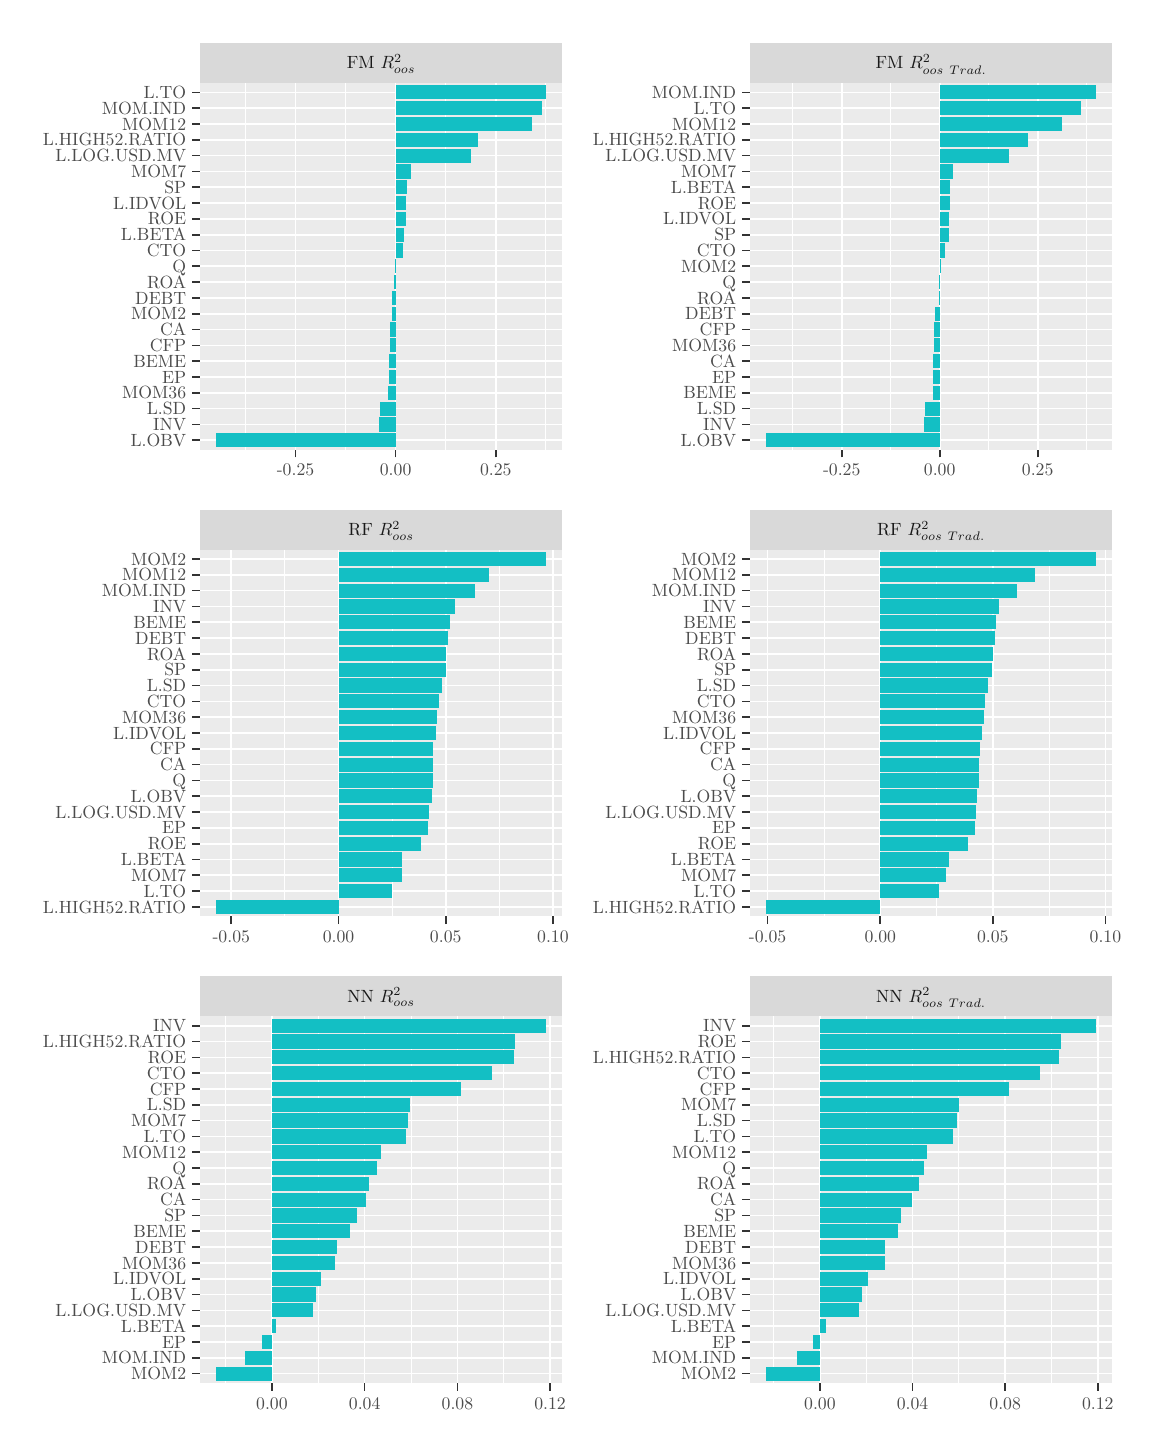
\begin{tikzpicture}[x=1pt,y=1pt]
\definecolor{fillColor}{RGB}{255,255,255}
\path[use as bounding box,fill=fillColor,fill opacity=0.00] (0,0) rectangle (397.48,505.89);
\begin{scope}
\path[clip] (  0.00,337.26) rectangle (198.74,505.89);
\definecolor{drawColor}{RGB}{255,255,255}
\definecolor{fillColor}{RGB}{255,255,255}

\path[draw=drawColor,line width= 0.6pt,line join=round,line cap=round,fill=fillColor] (  0.00,337.26) rectangle (198.74,505.89);
\end{scope}
\begin{scope}
\path[clip] ( 62.22,353.36) rectangle (193.24,485.94);
\definecolor{fillColor}{gray}{0.92}

\path[fill=fillColor] ( 62.22,353.36) rectangle (193.24,485.94);
\definecolor{drawColor}{RGB}{255,255,255}

\path[draw=drawColor,line width= 0.3pt,line join=round] ( 78.70,353.36) --
	( 78.70,485.94);

\path[draw=drawColor,line width= 0.3pt,line join=round] (114.88,353.36) --
	(114.88,485.94);

\path[draw=drawColor,line width= 0.3pt,line join=round] (151.05,353.36) --
	(151.05,485.94);

\path[draw=drawColor,line width= 0.3pt,line join=round] (187.23,353.36) --
	(187.23,485.94);

\path[draw=drawColor,line width= 0.6pt,line join=round] ( 62.22,356.79) --
	(193.24,356.79);

\path[draw=drawColor,line width= 0.6pt,line join=round] ( 62.22,362.51) --
	(193.24,362.51);

\path[draw=drawColor,line width= 0.6pt,line join=round] ( 62.22,368.22) --
	(193.24,368.22);

\path[draw=drawColor,line width= 0.6pt,line join=round] ( 62.22,373.93) --
	(193.24,373.93);

\path[draw=drawColor,line width= 0.6pt,line join=round] ( 62.22,379.65) --
	(193.24,379.65);

\path[draw=drawColor,line width= 0.6pt,line join=round] ( 62.22,385.36) --
	(193.24,385.36);

\path[draw=drawColor,line width= 0.6pt,line join=round] ( 62.22,391.08) --
	(193.24,391.08);

\path[draw=drawColor,line width= 0.6pt,line join=round] ( 62.22,396.79) --
	(193.24,396.79);

\path[draw=drawColor,line width= 0.6pt,line join=round] ( 62.22,402.51) --
	(193.24,402.51);

\path[draw=drawColor,line width= 0.6pt,line join=round] ( 62.22,408.22) --
	(193.24,408.22);

\path[draw=drawColor,line width= 0.6pt,line join=round] ( 62.22,413.94) --
	(193.24,413.94);

\path[draw=drawColor,line width= 0.6pt,line join=round] ( 62.22,419.65) --
	(193.24,419.65);

\path[draw=drawColor,line width= 0.6pt,line join=round] ( 62.22,425.36) --
	(193.24,425.36);

\path[draw=drawColor,line width= 0.6pt,line join=round] ( 62.22,431.08) --
	(193.24,431.08);

\path[draw=drawColor,line width= 0.6pt,line join=round] ( 62.22,436.79) --
	(193.24,436.79);

\path[draw=drawColor,line width= 0.6pt,line join=round] ( 62.22,442.51) --
	(193.24,442.51);

\path[draw=drawColor,line width= 0.6pt,line join=round] ( 62.22,448.22) --
	(193.24,448.22);

\path[draw=drawColor,line width= 0.6pt,line join=round] ( 62.22,453.94) --
	(193.24,453.94);

\path[draw=drawColor,line width= 0.6pt,line join=round] ( 62.22,459.65) --
	(193.24,459.65);

\path[draw=drawColor,line width= 0.6pt,line join=round] ( 62.22,465.37) --
	(193.24,465.37);

\path[draw=drawColor,line width= 0.6pt,line join=round] ( 62.22,471.08) --
	(193.24,471.08);

\path[draw=drawColor,line width= 0.6pt,line join=round] ( 62.22,476.79) --
	(193.24,476.79);

\path[draw=drawColor,line width= 0.6pt,line join=round] ( 62.22,482.51) --
	(193.24,482.51);

\path[draw=drawColor,line width= 0.6pt,line join=round] ( 96.79,353.36) --
	( 96.79,485.94);

\path[draw=drawColor,line width= 0.6pt,line join=round] (132.96,353.36) --
	(132.96,485.94);

\path[draw=drawColor,line width= 0.6pt,line join=round] (169.14,353.36) --
	(169.14,485.94);
\definecolor{fillColor}{RGB}{19,191,196}

\path[fill=fillColor] (130.99,394.22) rectangle (132.96,399.36);

\path[fill=fillColor] (132.96,422.79) rectangle (135.58,427.94);

\path[fill=fillColor] (130.56,382.79) rectangle (132.96,387.93);

\path[fill=fillColor] (130.92,388.51) rectangle (132.96,393.65);

\path[fill=fillColor] (126.96,359.93) rectangle (132.96,365.08);

\path[fill=fillColor] (131.76,405.65) rectangle (132.96,410.79);

\path[fill=fillColor] (132.96,445.65) rectangle (136.90,450.79);

\path[fill=fillColor] (130.49,377.08) rectangle (132.96,382.22);

\path[fill=fillColor] (132.55,411.36) rectangle (132.96,416.51);

\path[fill=fillColor] (132.96,434.22) rectangle (136.57,439.36);

\path[fill=fillColor] (132.90,417.08) rectangle (132.96,422.22);

\path[fill=fillColor] (132.96,451.37) rectangle (138.34,456.51);

\path[fill=fillColor] (132.96,468.51) rectangle (182.41,473.65);

\path[fill=fillColor] (130.38,371.36) rectangle (132.96,376.51);

\path[fill=fillColor] (131.63,399.94) rectangle (132.96,405.08);

\path[fill=fillColor] (132.96,474.22) rectangle (185.98,479.37);

\path[fill=fillColor] (127.27,365.65) rectangle (132.96,370.79);

\path[fill=fillColor] (132.96,462.79) rectangle (162.64,467.94);

\path[fill=fillColor] (132.96,428.51) rectangle (135.89,433.65);

\path[fill=fillColor] (132.96,439.94) rectangle (136.60,445.08);

\path[fill=fillColor] (132.96,457.08) rectangle (160.11,462.22);

\path[fill=fillColor] (132.96,479.94) rectangle (187.29,485.08);

\path[fill=fillColor] ( 68.17,354.22) rectangle (132.96,359.36);
\end{scope}
\begin{scope}
\path[clip] ( 62.22,485.94) rectangle (193.24,500.39);
\definecolor{fillColor}{gray}{0.85}

\path[fill=fillColor] ( 62.22,485.94) rectangle (193.24,500.39);
\definecolor{drawColor}{gray}{0.10}

\node[text=drawColor,anchor=base,inner sep=0pt, outer sep=0pt, scale=  0.64] at (127.73,490.96) {FM $R^2_{oos}$};
\end{scope}
\begin{scope}
\path[clip] (  0.00,  0.00) rectangle (397.48,505.89);
\definecolor{drawColor}{gray}{0.20}

\path[draw=drawColor,line width= 0.6pt,line join=round] ( 96.79,350.61) --
	( 96.79,353.36);

\path[draw=drawColor,line width= 0.6pt,line join=round] (132.96,350.61) --
	(132.96,353.36);

\path[draw=drawColor,line width= 0.6pt,line join=round] (169.14,350.61) --
	(169.14,353.36);
\end{scope}
\begin{scope}
\path[clip] (  0.00,  0.00) rectangle (397.48,505.89);
\definecolor{drawColor}{gray}{0.30}

\node[text=drawColor,anchor=base,inner sep=0pt, outer sep=0pt, scale=  0.64] at ( 96.79,344.00) {-0.25};

\node[text=drawColor,anchor=base,inner sep=0pt, outer sep=0pt, scale=  0.64] at (132.96,344.00) {0.00};

\node[text=drawColor,anchor=base,inner sep=0pt, outer sep=0pt, scale=  0.64] at (169.14,344.00) {0.25};
\end{scope}
\begin{scope}
\path[clip] (  0.00,  0.00) rectangle (397.48,505.89);
\definecolor{drawColor}{gray}{0.30}

\node[text=drawColor,anchor=base east,inner sep=0pt, outer sep=0pt, scale=  0.64] at ( 57.27,354.59) {L.OBV};

\node[text=drawColor,anchor=base east,inner sep=0pt, outer sep=0pt, scale=  0.64] at ( 57.27,360.30) {INV};

\node[text=drawColor,anchor=base east,inner sep=0pt, outer sep=0pt, scale=  0.64] at ( 57.27,366.02) {L.SD};

\node[text=drawColor,anchor=base east,inner sep=0pt, outer sep=0pt, scale=  0.64] at ( 57.27,371.73) {MOM36};

\node[text=drawColor,anchor=base east,inner sep=0pt, outer sep=0pt, scale=  0.64] at ( 57.27,377.44) {EP};

\node[text=drawColor,anchor=base east,inner sep=0pt, outer sep=0pt, scale=  0.64] at ( 57.27,383.16) {BEME};

\node[text=drawColor,anchor=base east,inner sep=0pt, outer sep=0pt, scale=  0.64] at ( 57.27,388.87) {CFP};

\node[text=drawColor,anchor=base east,inner sep=0pt, outer sep=0pt, scale=  0.64] at ( 57.27,394.59) {CA};

\node[text=drawColor,anchor=base east,inner sep=0pt, outer sep=0pt, scale=  0.64] at ( 57.27,400.30) {MOM2};

\node[text=drawColor,anchor=base east,inner sep=0pt, outer sep=0pt, scale=  0.64] at ( 57.27,406.02) {DEBT};

\node[text=drawColor,anchor=base east,inner sep=0pt, outer sep=0pt, scale=  0.64] at ( 57.27,411.73) {ROA};

\node[text=drawColor,anchor=base east,inner sep=0pt, outer sep=0pt, scale=  0.64] at ( 57.27,417.45) {Q};

\node[text=drawColor,anchor=base east,inner sep=0pt, outer sep=0pt, scale=  0.64] at ( 57.27,423.16) {CTO};

\node[text=drawColor,anchor=base east,inner sep=0pt, outer sep=0pt, scale=  0.64] at ( 57.27,428.88) {L.BETA};

\node[text=drawColor,anchor=base east,inner sep=0pt, outer sep=0pt, scale=  0.64] at ( 57.27,434.59) {ROE};

\node[text=drawColor,anchor=base east,inner sep=0pt, outer sep=0pt, scale=  0.64] at ( 57.27,440.30) {L.IDVOL};

\node[text=drawColor,anchor=base east,inner sep=0pt, outer sep=0pt, scale=  0.64] at ( 57.27,446.02) {SP};

\node[text=drawColor,anchor=base east,inner sep=0pt, outer sep=0pt, scale=  0.64] at ( 57.27,451.73) {MOM7};

\node[text=drawColor,anchor=base east,inner sep=0pt, outer sep=0pt, scale=  0.64] at ( 57.27,457.45) {L.LOG.USD.MV};

\node[text=drawColor,anchor=base east,inner sep=0pt, outer sep=0pt, scale=  0.64] at ( 57.27,463.16) {L.HIGH52.RATIO};

\node[text=drawColor,anchor=base east,inner sep=0pt, outer sep=0pt, scale=  0.64] at ( 57.27,468.88) {MOM12};

\node[text=drawColor,anchor=base east,inner sep=0pt, outer sep=0pt, scale=  0.64] at ( 57.27,474.59) {MOM.IND};

\node[text=drawColor,anchor=base east,inner sep=0pt, outer sep=0pt, scale=  0.64] at ( 57.27,480.31) {L.TO};
\end{scope}
\begin{scope}
\path[clip] (  0.00,  0.00) rectangle (397.48,505.89);
\definecolor{drawColor}{gray}{0.20}

\path[draw=drawColor,line width= 0.6pt,line join=round] ( 59.47,356.79) --
	( 62.22,356.79);

\path[draw=drawColor,line width= 0.6pt,line join=round] ( 59.47,362.51) --
	( 62.22,362.51);

\path[draw=drawColor,line width= 0.6pt,line join=round] ( 59.47,368.22) --
	( 62.22,368.22);

\path[draw=drawColor,line width= 0.6pt,line join=round] ( 59.47,373.93) --
	( 62.22,373.93);

\path[draw=drawColor,line width= 0.6pt,line join=round] ( 59.47,379.65) --
	( 62.22,379.65);

\path[draw=drawColor,line width= 0.6pt,line join=round] ( 59.47,385.36) --
	( 62.22,385.36);

\path[draw=drawColor,line width= 0.6pt,line join=round] ( 59.47,391.08) --
	( 62.22,391.08);

\path[draw=drawColor,line width= 0.6pt,line join=round] ( 59.47,396.79) --
	( 62.22,396.79);

\path[draw=drawColor,line width= 0.6pt,line join=round] ( 59.47,402.51) --
	( 62.22,402.51);

\path[draw=drawColor,line width= 0.6pt,line join=round] ( 59.47,408.22) --
	( 62.22,408.22);

\path[draw=drawColor,line width= 0.6pt,line join=round] ( 59.47,413.94) --
	( 62.22,413.94);

\path[draw=drawColor,line width= 0.6pt,line join=round] ( 59.47,419.65) --
	( 62.22,419.65);

\path[draw=drawColor,line width= 0.6pt,line join=round] ( 59.47,425.36) --
	( 62.22,425.36);

\path[draw=drawColor,line width= 0.6pt,line join=round] ( 59.47,431.08) --
	( 62.22,431.08);

\path[draw=drawColor,line width= 0.6pt,line join=round] ( 59.47,436.79) --
	( 62.22,436.79);

\path[draw=drawColor,line width= 0.6pt,line join=round] ( 59.47,442.51) --
	( 62.22,442.51);

\path[draw=drawColor,line width= 0.6pt,line join=round] ( 59.47,448.22) --
	( 62.22,448.22);

\path[draw=drawColor,line width= 0.6pt,line join=round] ( 59.47,453.94) --
	( 62.22,453.94);

\path[draw=drawColor,line width= 0.6pt,line join=round] ( 59.47,459.65) --
	( 62.22,459.65);

\path[draw=drawColor,line width= 0.6pt,line join=round] ( 59.47,465.37) --
	( 62.22,465.37);

\path[draw=drawColor,line width= 0.6pt,line join=round] ( 59.47,471.08) --
	( 62.22,471.08);

\path[draw=drawColor,line width= 0.6pt,line join=round] ( 59.47,476.79) --
	( 62.22,476.79);

\path[draw=drawColor,line width= 0.6pt,line join=round] ( 59.47,482.51) --
	( 62.22,482.51);
\end{scope}
\begin{scope}
\path[clip] (198.74,337.26) rectangle (397.48,505.89);
\definecolor{drawColor}{RGB}{255,255,255}
\definecolor{fillColor}{RGB}{255,255,255}

\path[draw=drawColor,line width= 0.6pt,line join=round,line cap=round,fill=fillColor] (198.74,337.26) rectangle (397.48,505.89);
\end{scope}
\begin{scope}
\path[clip] (260.96,353.36) rectangle (391.98,485.94);
\definecolor{fillColor}{gray}{0.92}

\path[fill=fillColor] (260.96,353.36) rectangle (391.98,485.94);
\definecolor{drawColor}{RGB}{255,255,255}

\path[draw=drawColor,line width= 0.3pt,line join=round] (276.46,353.36) --
	(276.46,485.94);

\path[draw=drawColor,line width= 0.3pt,line join=round] (311.86,353.36) --
	(311.86,485.94);

\path[draw=drawColor,line width= 0.3pt,line join=round] (347.26,353.36) --
	(347.26,485.94);

\path[draw=drawColor,line width= 0.3pt,line join=round] (382.66,353.36) --
	(382.66,485.94);

\path[draw=drawColor,line width= 0.6pt,line join=round] (260.96,356.79) --
	(391.98,356.79);

\path[draw=drawColor,line width= 0.6pt,line join=round] (260.96,362.51) --
	(391.98,362.51);

\path[draw=drawColor,line width= 0.6pt,line join=round] (260.96,368.22) --
	(391.98,368.22);

\path[draw=drawColor,line width= 0.6pt,line join=round] (260.96,373.93) --
	(391.98,373.93);

\path[draw=drawColor,line width= 0.6pt,line join=round] (260.96,379.65) --
	(391.98,379.65);

\path[draw=drawColor,line width= 0.6pt,line join=round] (260.96,385.36) --
	(391.98,385.36);

\path[draw=drawColor,line width= 0.6pt,line join=round] (260.96,391.08) --
	(391.98,391.08);

\path[draw=drawColor,line width= 0.6pt,line join=round] (260.96,396.79) --
	(391.98,396.79);

\path[draw=drawColor,line width= 0.6pt,line join=round] (260.96,402.51) --
	(391.98,402.51);

\path[draw=drawColor,line width= 0.6pt,line join=round] (260.96,408.22) --
	(391.98,408.22);

\path[draw=drawColor,line width= 0.6pt,line join=round] (260.96,413.94) --
	(391.98,413.94);

\path[draw=drawColor,line width= 0.6pt,line join=round] (260.96,419.65) --
	(391.98,419.65);

\path[draw=drawColor,line width= 0.6pt,line join=round] (260.96,425.36) --
	(391.98,425.36);

\path[draw=drawColor,line width= 0.6pt,line join=round] (260.96,431.08) --
	(391.98,431.08);

\path[draw=drawColor,line width= 0.6pt,line join=round] (260.96,436.79) --
	(391.98,436.79);

\path[draw=drawColor,line width= 0.6pt,line join=round] (260.96,442.51) --
	(391.98,442.51);

\path[draw=drawColor,line width= 0.6pt,line join=round] (260.96,448.22) --
	(391.98,448.22);

\path[draw=drawColor,line width= 0.6pt,line join=round] (260.96,453.94) --
	(391.98,453.94);

\path[draw=drawColor,line width= 0.6pt,line join=round] (260.96,459.65) --
	(391.98,459.65);

\path[draw=drawColor,line width= 0.6pt,line join=round] (260.96,465.37) --
	(391.98,465.37);

\path[draw=drawColor,line width= 0.6pt,line join=round] (260.96,471.08) --
	(391.98,471.08);

\path[draw=drawColor,line width= 0.6pt,line join=round] (260.96,476.79) --
	(391.98,476.79);

\path[draw=drawColor,line width= 0.6pt,line join=round] (260.96,482.51) --
	(391.98,482.51);

\path[draw=drawColor,line width= 0.6pt,line join=round] (294.16,353.36) --
	(294.16,485.94);

\path[draw=drawColor,line width= 0.6pt,line join=round] (329.56,353.36) --
	(329.56,485.94);

\path[draw=drawColor,line width= 0.6pt,line join=round] (364.96,353.36) --
	(364.96,485.94);
\definecolor{fillColor}{RGB}{19,191,196}

\path[fill=fillColor] (327.28,382.79) rectangle (329.56,387.93);

\path[fill=fillColor] (329.56,422.79) rectangle (331.30,427.94);

\path[fill=fillColor] (326.97,371.36) rectangle (329.56,376.51);

\path[fill=fillColor] (327.50,394.22) rectangle (329.56,399.36);

\path[fill=fillColor] (323.82,359.93) rectangle (329.56,365.08);

\path[fill=fillColor] (328.01,399.94) rectangle (329.56,405.08);

\path[fill=fillColor] (329.56,428.51) rectangle (332.74,433.65);

\path[fill=fillColor] (327.02,377.08) rectangle (329.56,382.22);

\path[fill=fillColor] (329.26,405.65) rectangle (329.56,410.79);

\path[fill=fillColor] (329.56,439.94) rectangle (333.14,445.08);

\path[fill=fillColor] (329.45,411.36) rectangle (329.56,416.51);

\path[fill=fillColor] (329.56,451.37) rectangle (334.30,456.51);

\path[fill=fillColor] (329.56,468.51) rectangle (373.74,473.65);

\path[fill=fillColor] (327.45,388.51) rectangle (329.56,393.65);

\path[fill=fillColor] (329.56,417.08) rectangle (329.67,422.22);

\path[fill=fillColor] (329.56,479.94) rectangle (386.03,485.08);

\path[fill=fillColor] (324.37,365.65) rectangle (329.56,370.79);

\path[fill=fillColor] (329.56,462.79) rectangle (361.64,467.94);

\path[fill=fillColor] (329.56,445.65) rectangle (333.22,450.79);

\path[fill=fillColor] (329.56,434.22) rectangle (332.74,439.36);

\path[fill=fillColor] (329.56,457.08) rectangle (354.48,462.22);

\path[fill=fillColor] (329.56,474.22) rectangle (380.48,479.37);

\path[fill=fillColor] (266.91,354.22) rectangle (329.56,359.36);
\end{scope}
\begin{scope}
\path[clip] (260.96,485.94) rectangle (391.98,500.39);
\definecolor{fillColor}{gray}{0.85}

\path[fill=fillColor] (260.96,485.94) rectangle (391.98,500.39);
\definecolor{drawColor}{gray}{0.10}

\node[text=drawColor,anchor=base,inner sep=0pt, outer sep=0pt, scale=  0.64] at (326.47,490.96) {FM $R^2_{oos \ Trad.}$};
\end{scope}
\begin{scope}
\path[clip] (  0.00,  0.00) rectangle (397.48,505.89);
\definecolor{drawColor}{gray}{0.20}

\path[draw=drawColor,line width= 0.6pt,line join=round] (294.16,350.61) --
	(294.16,353.36);

\path[draw=drawColor,line width= 0.6pt,line join=round] (329.56,350.61) --
	(329.56,353.36);

\path[draw=drawColor,line width= 0.6pt,line join=round] (364.96,350.61) --
	(364.96,353.36);
\end{scope}
\begin{scope}
\path[clip] (  0.00,  0.00) rectangle (397.48,505.89);
\definecolor{drawColor}{gray}{0.30}

\node[text=drawColor,anchor=base,inner sep=0pt, outer sep=0pt, scale=  0.64] at (294.16,344.00) {-0.25};

\node[text=drawColor,anchor=base,inner sep=0pt, outer sep=0pt, scale=  0.64] at (329.56,344.00) {0.00};

\node[text=drawColor,anchor=base,inner sep=0pt, outer sep=0pt, scale=  0.64] at (364.96,344.00) {0.25};
\end{scope}
\begin{scope}
\path[clip] (  0.00,  0.00) rectangle (397.48,505.89);
\definecolor{drawColor}{gray}{0.30}

\node[text=drawColor,anchor=base east,inner sep=0pt, outer sep=0pt, scale=  0.64] at (256.01,354.59) {L.OBV};

\node[text=drawColor,anchor=base east,inner sep=0pt, outer sep=0pt, scale=  0.64] at (256.01,360.30) {INV};

\node[text=drawColor,anchor=base east,inner sep=0pt, outer sep=0pt, scale=  0.64] at (256.01,366.02) {L.SD};

\node[text=drawColor,anchor=base east,inner sep=0pt, outer sep=0pt, scale=  0.64] at (256.01,371.73) {BEME};

\node[text=drawColor,anchor=base east,inner sep=0pt, outer sep=0pt, scale=  0.64] at (256.01,377.44) {EP};

\node[text=drawColor,anchor=base east,inner sep=0pt, outer sep=0pt, scale=  0.64] at (256.01,383.16) {CA};

\node[text=drawColor,anchor=base east,inner sep=0pt, outer sep=0pt, scale=  0.64] at (256.01,388.87) {MOM36};

\node[text=drawColor,anchor=base east,inner sep=0pt, outer sep=0pt, scale=  0.64] at (256.01,394.59) {CFP};

\node[text=drawColor,anchor=base east,inner sep=0pt, outer sep=0pt, scale=  0.64] at (256.01,400.30) {DEBT};

\node[text=drawColor,anchor=base east,inner sep=0pt, outer sep=0pt, scale=  0.64] at (256.01,406.02) {ROA};

\node[text=drawColor,anchor=base east,inner sep=0pt, outer sep=0pt, scale=  0.64] at (256.01,411.73) {Q};

\node[text=drawColor,anchor=base east,inner sep=0pt, outer sep=0pt, scale=  0.64] at (256.01,417.45) {MOM2};

\node[text=drawColor,anchor=base east,inner sep=0pt, outer sep=0pt, scale=  0.64] at (256.01,423.16) {CTO};

\node[text=drawColor,anchor=base east,inner sep=0pt, outer sep=0pt, scale=  0.64] at (256.01,428.88) {SP};

\node[text=drawColor,anchor=base east,inner sep=0pt, outer sep=0pt, scale=  0.64] at (256.01,434.59) {L.IDVOL};

\node[text=drawColor,anchor=base east,inner sep=0pt, outer sep=0pt, scale=  0.64] at (256.01,440.30) {ROE};

\node[text=drawColor,anchor=base east,inner sep=0pt, outer sep=0pt, scale=  0.64] at (256.01,446.02) {L.BETA};

\node[text=drawColor,anchor=base east,inner sep=0pt, outer sep=0pt, scale=  0.64] at (256.01,451.73) {MOM7};

\node[text=drawColor,anchor=base east,inner sep=0pt, outer sep=0pt, scale=  0.64] at (256.01,457.45) {L.LOG.USD.MV};

\node[text=drawColor,anchor=base east,inner sep=0pt, outer sep=0pt, scale=  0.64] at (256.01,463.16) {L.HIGH52.RATIO};

\node[text=drawColor,anchor=base east,inner sep=0pt, outer sep=0pt, scale=  0.64] at (256.01,468.88) {MOM12};

\node[text=drawColor,anchor=base east,inner sep=0pt, outer sep=0pt, scale=  0.64] at (256.01,474.59) {L.TO};

\node[text=drawColor,anchor=base east,inner sep=0pt, outer sep=0pt, scale=  0.64] at (256.01,480.31) {MOM.IND};
\end{scope}
\begin{scope}
\path[clip] (  0.00,  0.00) rectangle (397.48,505.89);
\definecolor{drawColor}{gray}{0.20}

\path[draw=drawColor,line width= 0.6pt,line join=round] (258.21,356.79) --
	(260.96,356.79);

\path[draw=drawColor,line width= 0.6pt,line join=round] (258.21,362.51) --
	(260.96,362.51);

\path[draw=drawColor,line width= 0.6pt,line join=round] (258.21,368.22) --
	(260.96,368.22);

\path[draw=drawColor,line width= 0.6pt,line join=round] (258.21,373.93) --
	(260.96,373.93);

\path[draw=drawColor,line width= 0.6pt,line join=round] (258.21,379.65) --
	(260.96,379.65);

\path[draw=drawColor,line width= 0.6pt,line join=round] (258.21,385.36) --
	(260.96,385.36);

\path[draw=drawColor,line width= 0.6pt,line join=round] (258.21,391.08) --
	(260.96,391.08);

\path[draw=drawColor,line width= 0.6pt,line join=round] (258.21,396.79) --
	(260.96,396.79);

\path[draw=drawColor,line width= 0.6pt,line join=round] (258.21,402.51) --
	(260.96,402.51);

\path[draw=drawColor,line width= 0.6pt,line join=round] (258.21,408.22) --
	(260.96,408.22);

\path[draw=drawColor,line width= 0.6pt,line join=round] (258.21,413.94) --
	(260.96,413.94);

\path[draw=drawColor,line width= 0.6pt,line join=round] (258.21,419.65) --
	(260.96,419.65);

\path[draw=drawColor,line width= 0.6pt,line join=round] (258.21,425.36) --
	(260.96,425.36);

\path[draw=drawColor,line width= 0.6pt,line join=round] (258.21,431.08) --
	(260.96,431.08);

\path[draw=drawColor,line width= 0.6pt,line join=round] (258.21,436.79) --
	(260.96,436.79);

\path[draw=drawColor,line width= 0.6pt,line join=round] (258.21,442.51) --
	(260.96,442.51);

\path[draw=drawColor,line width= 0.6pt,line join=round] (258.21,448.22) --
	(260.96,448.22);

\path[draw=drawColor,line width= 0.6pt,line join=round] (258.21,453.94) --
	(260.96,453.94);

\path[draw=drawColor,line width= 0.6pt,line join=round] (258.21,459.65) --
	(260.96,459.65);

\path[draw=drawColor,line width= 0.6pt,line join=round] (258.21,465.37) --
	(260.96,465.37);

\path[draw=drawColor,line width= 0.6pt,line join=round] (258.21,471.08) --
	(260.96,471.08);

\path[draw=drawColor,line width= 0.6pt,line join=round] (258.21,476.79) --
	(260.96,476.79);

\path[draw=drawColor,line width= 0.6pt,line join=round] (258.21,482.51) --
	(260.96,482.51);
\end{scope}
\begin{scope}
\path[clip] (  0.00,168.63) rectangle (198.74,337.26);
\definecolor{drawColor}{RGB}{255,255,255}
\definecolor{fillColor}{RGB}{255,255,255}

\path[draw=drawColor,line width= 0.6pt,line join=round,line cap=round,fill=fillColor] (  0.00,168.63) rectangle (198.74,337.26);
\end{scope}
\begin{scope}
\path[clip] ( 62.22,184.73) rectangle (193.24,317.31);
\definecolor{fillColor}{gray}{0.92}

\path[fill=fillColor] ( 62.22,184.73) rectangle (193.24,317.31);
\definecolor{drawColor}{RGB}{255,255,255}

\path[draw=drawColor,line width= 0.3pt,line join=round] ( 92.94,184.73) --
	( 92.94,317.31);

\path[draw=drawColor,line width= 0.3pt,line join=round] (131.69,184.73) --
	(131.69,317.31);

\path[draw=drawColor,line width= 0.3pt,line join=round] (170.43,184.73) --
	(170.43,317.31);

\path[draw=drawColor,line width= 0.6pt,line join=round] ( 62.22,188.16) --
	(193.24,188.16);

\path[draw=drawColor,line width= 0.6pt,line join=round] ( 62.22,193.88) --
	(193.24,193.88);

\path[draw=drawColor,line width= 0.6pt,line join=round] ( 62.22,199.59) --
	(193.24,199.59);

\path[draw=drawColor,line width= 0.6pt,line join=round] ( 62.22,205.30) --
	(193.24,205.30);

\path[draw=drawColor,line width= 0.6pt,line join=round] ( 62.22,211.02) --
	(193.24,211.02);

\path[draw=drawColor,line width= 0.6pt,line join=round] ( 62.22,216.73) --
	(193.24,216.73);

\path[draw=drawColor,line width= 0.6pt,line join=round] ( 62.22,222.45) --
	(193.24,222.45);

\path[draw=drawColor,line width= 0.6pt,line join=round] ( 62.22,228.16) --
	(193.24,228.16);

\path[draw=drawColor,line width= 0.6pt,line join=round] ( 62.22,233.88) --
	(193.24,233.88);

\path[draw=drawColor,line width= 0.6pt,line join=round] ( 62.22,239.59) --
	(193.24,239.59);

\path[draw=drawColor,line width= 0.6pt,line join=round] ( 62.22,245.31) --
	(193.24,245.31);

\path[draw=drawColor,line width= 0.6pt,line join=round] ( 62.22,251.02) --
	(193.24,251.02);

\path[draw=drawColor,line width= 0.6pt,line join=round] ( 62.22,256.73) --
	(193.24,256.73);

\path[draw=drawColor,line width= 0.6pt,line join=round] ( 62.22,262.45) --
	(193.24,262.45);

\path[draw=drawColor,line width= 0.6pt,line join=round] ( 62.22,268.16) --
	(193.24,268.16);

\path[draw=drawColor,line width= 0.6pt,line join=round] ( 62.22,273.88) --
	(193.24,273.88);

\path[draw=drawColor,line width= 0.6pt,line join=round] ( 62.22,279.59) --
	(193.24,279.59);

\path[draw=drawColor,line width= 0.6pt,line join=round] ( 62.22,285.31) --
	(193.24,285.31);

\path[draw=drawColor,line width= 0.6pt,line join=round] ( 62.22,291.02) --
	(193.24,291.02);

\path[draw=drawColor,line width= 0.6pt,line join=round] ( 62.22,296.74) --
	(193.24,296.74);

\path[draw=drawColor,line width= 0.6pt,line join=round] ( 62.22,302.45) --
	(193.24,302.45);

\path[draw=drawColor,line width= 0.6pt,line join=round] ( 62.22,308.16) --
	(193.24,308.16);

\path[draw=drawColor,line width= 0.6pt,line join=round] ( 62.22,313.88) --
	(193.24,313.88);

\path[draw=drawColor,line width= 0.6pt,line join=round] ( 73.57,184.73) --
	( 73.57,317.31);

\path[draw=drawColor,line width= 0.6pt,line join=round] (112.32,184.73) --
	(112.32,317.31);

\path[draw=drawColor,line width= 0.6pt,line join=round] (151.06,184.73) --
	(151.06,317.31);

\path[draw=drawColor,line width= 0.6pt,line join=round] (189.80,184.73) --
	(189.80,317.31);
\definecolor{fillColor}{RGB}{19,191,196}

\path[fill=fillColor] (112.32,237.02) rectangle (146.46,242.16);

\path[fill=fillColor] (112.32,259.88) rectangle (148.61,265.02);

\path[fill=fillColor] (112.32,288.45) rectangle (152.56,293.59);

\path[fill=fillColor] (112.32,242.73) rectangle (146.60,247.88);

\path[fill=fillColor] (112.32,294.16) rectangle (154.34,299.31);

\path[fill=fillColor] (112.32,282.74) rectangle (151.74,287.88);

\path[fill=fillColor] (112.32,271.31) rectangle (150.98,276.45);

\path[fill=fillColor] (112.32,214.16) rectangle (144.56,219.30);

\path[fill=fillColor] (112.32,277.02) rectangle (151.26,282.16);

\path[fill=fillColor] (112.32,208.45) rectangle (142.07,213.59);

\path[fill=fillColor] (112.32,231.31) rectangle (146.43,236.45);

\path[fill=fillColor] (112.32,197.02) rectangle (135.23,202.16);

\path[fill=fillColor] (112.32,305.59) rectangle (166.77,310.74);

\path[fill=fillColor] (112.32,254.16) rectangle (147.96,259.31);

\path[fill=fillColor] (112.32,311.31) rectangle (187.29,316.45);

\path[fill=fillColor] (112.32,299.88) rectangle (161.81,305.02);

\path[fill=fillColor] (112.32,265.59) rectangle (149.65,270.73);

\path[fill=fillColor] ( 68.17,185.59) rectangle (112.32,190.73);

\path[fill=fillColor] (112.32,202.73) rectangle (135.32,207.88);

\path[fill=fillColor] (112.32,248.45) rectangle (147.66,253.59);

\path[fill=fillColor] (112.32,219.88) rectangle (144.90,225.02);

\path[fill=fillColor] (112.32,191.30) rectangle (131.70,196.45);

\path[fill=fillColor] (112.32,225.59) rectangle (145.98,230.73);
\end{scope}
\begin{scope}
\path[clip] ( 62.22,317.31) rectangle (193.24,331.76);
\definecolor{fillColor}{gray}{0.85}

\path[fill=fillColor] ( 62.22,317.31) rectangle (193.24,331.76);
\definecolor{drawColor}{gray}{0.10}

\node[text=drawColor,anchor=base,inner sep=0pt, outer sep=0pt, scale=  0.64] at (127.73,322.33) {RF $R^2_{oos}$};
\end{scope}
\begin{scope}
\path[clip] (  0.00,  0.00) rectangle (397.48,505.89);
\definecolor{drawColor}{gray}{0.20}

\path[draw=drawColor,line width= 0.6pt,line join=round] ( 73.57,181.98) --
	( 73.57,184.73);

\path[draw=drawColor,line width= 0.6pt,line join=round] (112.32,181.98) --
	(112.32,184.73);

\path[draw=drawColor,line width= 0.6pt,line join=round] (151.06,181.98) --
	(151.06,184.73);

\path[draw=drawColor,line width= 0.6pt,line join=round] (189.80,181.98) --
	(189.80,184.73);
\end{scope}
\begin{scope}
\path[clip] (  0.00,  0.00) rectangle (397.48,505.89);
\definecolor{drawColor}{gray}{0.30}

\node[text=drawColor,anchor=base,inner sep=0pt, outer sep=0pt, scale=  0.64] at ( 73.57,175.37) {-0.05};

\node[text=drawColor,anchor=base,inner sep=0pt, outer sep=0pt, scale=  0.64] at (112.32,175.37) {0.00};

\node[text=drawColor,anchor=base,inner sep=0pt, outer sep=0pt, scale=  0.64] at (151.06,175.37) {0.05};

\node[text=drawColor,anchor=base,inner sep=0pt, outer sep=0pt, scale=  0.64] at (189.80,175.37) {0.10};
\end{scope}
\begin{scope}
\path[clip] (  0.00,  0.00) rectangle (397.48,505.89);
\definecolor{drawColor}{gray}{0.30}

\node[text=drawColor,anchor=base east,inner sep=0pt, outer sep=0pt, scale=  0.64] at ( 57.27,185.96) {L.HIGH52.RATIO};

\node[text=drawColor,anchor=base east,inner sep=0pt, outer sep=0pt, scale=  0.64] at ( 57.27,191.67) {L.TO};

\node[text=drawColor,anchor=base east,inner sep=0pt, outer sep=0pt, scale=  0.64] at ( 57.27,197.39) {MOM7};

\node[text=drawColor,anchor=base east,inner sep=0pt, outer sep=0pt, scale=  0.64] at ( 57.27,203.10) {L.BETA};

\node[text=drawColor,anchor=base east,inner sep=0pt, outer sep=0pt, scale=  0.64] at ( 57.27,208.81) {ROE};

\node[text=drawColor,anchor=base east,inner sep=0pt, outer sep=0pt, scale=  0.64] at ( 57.27,214.53) {EP};

\node[text=drawColor,anchor=base east,inner sep=0pt, outer sep=0pt, scale=  0.64] at ( 57.27,220.24) {L.LOG.USD.MV};

\node[text=drawColor,anchor=base east,inner sep=0pt, outer sep=0pt, scale=  0.64] at ( 57.27,225.96) {L.OBV};

\node[text=drawColor,anchor=base east,inner sep=0pt, outer sep=0pt, scale=  0.64] at ( 57.27,231.67) {Q};

\node[text=drawColor,anchor=base east,inner sep=0pt, outer sep=0pt, scale=  0.64] at ( 57.27,237.39) {CA};

\node[text=drawColor,anchor=base east,inner sep=0pt, outer sep=0pt, scale=  0.64] at ( 57.27,243.10) {CFP};

\node[text=drawColor,anchor=base east,inner sep=0pt, outer sep=0pt, scale=  0.64] at ( 57.27,248.82) {L.IDVOL};

\node[text=drawColor,anchor=base east,inner sep=0pt, outer sep=0pt, scale=  0.64] at ( 57.27,254.53) {MOM36};

\node[text=drawColor,anchor=base east,inner sep=0pt, outer sep=0pt, scale=  0.64] at ( 57.27,260.25) {CTO};

\node[text=drawColor,anchor=base east,inner sep=0pt, outer sep=0pt, scale=  0.64] at ( 57.27,265.96) {L.SD};

\node[text=drawColor,anchor=base east,inner sep=0pt, outer sep=0pt, scale=  0.64] at ( 57.27,271.67) {SP};

\node[text=drawColor,anchor=base east,inner sep=0pt, outer sep=0pt, scale=  0.64] at ( 57.27,277.39) {ROA};

\node[text=drawColor,anchor=base east,inner sep=0pt, outer sep=0pt, scale=  0.64] at ( 57.27,283.10) {DEBT};

\node[text=drawColor,anchor=base east,inner sep=0pt, outer sep=0pt, scale=  0.64] at ( 57.27,288.82) {BEME};

\node[text=drawColor,anchor=base east,inner sep=0pt, outer sep=0pt, scale=  0.64] at ( 57.27,294.53) {INV};

\node[text=drawColor,anchor=base east,inner sep=0pt, outer sep=0pt, scale=  0.64] at ( 57.27,300.25) {MOM.IND};

\node[text=drawColor,anchor=base east,inner sep=0pt, outer sep=0pt, scale=  0.64] at ( 57.27,305.96) {MOM12};

\node[text=drawColor,anchor=base east,inner sep=0pt, outer sep=0pt, scale=  0.64] at ( 57.27,311.68) {MOM2};
\end{scope}
\begin{scope}
\path[clip] (  0.00,  0.00) rectangle (397.48,505.89);
\definecolor{drawColor}{gray}{0.20}

\path[draw=drawColor,line width= 0.6pt,line join=round] ( 59.47,188.16) --
	( 62.22,188.16);

\path[draw=drawColor,line width= 0.6pt,line join=round] ( 59.47,193.88) --
	( 62.22,193.88);

\path[draw=drawColor,line width= 0.6pt,line join=round] ( 59.47,199.59) --
	( 62.22,199.59);

\path[draw=drawColor,line width= 0.6pt,line join=round] ( 59.47,205.30) --
	( 62.22,205.30);

\path[draw=drawColor,line width= 0.6pt,line join=round] ( 59.47,211.02) --
	( 62.22,211.02);

\path[draw=drawColor,line width= 0.6pt,line join=round] ( 59.47,216.73) --
	( 62.22,216.73);

\path[draw=drawColor,line width= 0.6pt,line join=round] ( 59.47,222.45) --
	( 62.22,222.45);

\path[draw=drawColor,line width= 0.6pt,line join=round] ( 59.47,228.16) --
	( 62.22,228.16);

\path[draw=drawColor,line width= 0.6pt,line join=round] ( 59.47,233.88) --
	( 62.22,233.88);

\path[draw=drawColor,line width= 0.6pt,line join=round] ( 59.47,239.59) --
	( 62.22,239.59);

\path[draw=drawColor,line width= 0.6pt,line join=round] ( 59.47,245.31) --
	( 62.22,245.31);

\path[draw=drawColor,line width= 0.6pt,line join=round] ( 59.47,251.02) --
	( 62.22,251.02);

\path[draw=drawColor,line width= 0.6pt,line join=round] ( 59.47,256.73) --
	( 62.22,256.73);

\path[draw=drawColor,line width= 0.6pt,line join=round] ( 59.47,262.45) --
	( 62.22,262.45);

\path[draw=drawColor,line width= 0.6pt,line join=round] ( 59.47,268.16) --
	( 62.22,268.16);

\path[draw=drawColor,line width= 0.6pt,line join=round] ( 59.47,273.88) --
	( 62.22,273.88);

\path[draw=drawColor,line width= 0.6pt,line join=round] ( 59.47,279.59) --
	( 62.22,279.59);

\path[draw=drawColor,line width= 0.6pt,line join=round] ( 59.47,285.31) --
	( 62.22,285.31);

\path[draw=drawColor,line width= 0.6pt,line join=round] ( 59.47,291.02) --
	( 62.22,291.02);

\path[draw=drawColor,line width= 0.6pt,line join=round] ( 59.47,296.74) --
	( 62.22,296.74);

\path[draw=drawColor,line width= 0.6pt,line join=round] ( 59.47,302.45) --
	( 62.22,302.45);

\path[draw=drawColor,line width= 0.6pt,line join=round] ( 59.47,308.16) --
	( 62.22,308.16);

\path[draw=drawColor,line width= 0.6pt,line join=round] ( 59.47,313.88) --
	( 62.22,313.88);
\end{scope}
\begin{scope}
\path[clip] (198.74,168.63) rectangle (397.48,337.26);
\definecolor{drawColor}{RGB}{255,255,255}
\definecolor{fillColor}{RGB}{255,255,255}

\path[draw=drawColor,line width= 0.6pt,line join=round,line cap=round,fill=fillColor] (198.74,168.63) rectangle (397.48,337.26);
\end{scope}
\begin{scope}
\path[clip] (260.96,184.73) rectangle (391.98,317.31);
\definecolor{fillColor}{gray}{0.92}

\path[fill=fillColor] (260.96,184.73) rectangle (391.98,317.31);
\definecolor{drawColor}{RGB}{255,255,255}

\path[draw=drawColor,line width= 0.3pt,line join=round] (287.73,184.73) --
	(287.73,317.31);

\path[draw=drawColor,line width= 0.3pt,line join=round] (328.42,184.73) --
	(328.42,317.31);

\path[draw=drawColor,line width= 0.3pt,line join=round] (369.11,184.73) --
	(369.11,317.31);

\path[draw=drawColor,line width= 0.6pt,line join=round] (260.96,188.16) --
	(391.98,188.16);

\path[draw=drawColor,line width= 0.6pt,line join=round] (260.96,193.88) --
	(391.98,193.88);

\path[draw=drawColor,line width= 0.6pt,line join=round] (260.96,199.59) --
	(391.98,199.59);

\path[draw=drawColor,line width= 0.6pt,line join=round] (260.96,205.30) --
	(391.98,205.30);

\path[draw=drawColor,line width= 0.6pt,line join=round] (260.96,211.02) --
	(391.98,211.02);

\path[draw=drawColor,line width= 0.6pt,line join=round] (260.96,216.73) --
	(391.98,216.73);

\path[draw=drawColor,line width= 0.6pt,line join=round] (260.96,222.45) --
	(391.98,222.45);

\path[draw=drawColor,line width= 0.6pt,line join=round] (260.96,228.16) --
	(391.98,228.16);

\path[draw=drawColor,line width= 0.6pt,line join=round] (260.96,233.88) --
	(391.98,233.88);

\path[draw=drawColor,line width= 0.6pt,line join=round] (260.96,239.59) --
	(391.98,239.59);

\path[draw=drawColor,line width= 0.6pt,line join=round] (260.96,245.31) --
	(391.98,245.31);

\path[draw=drawColor,line width= 0.6pt,line join=round] (260.96,251.02) --
	(391.98,251.02);

\path[draw=drawColor,line width= 0.6pt,line join=round] (260.96,256.73) --
	(391.98,256.73);

\path[draw=drawColor,line width= 0.6pt,line join=round] (260.96,262.45) --
	(391.98,262.45);

\path[draw=drawColor,line width= 0.6pt,line join=round] (260.96,268.16) --
	(391.98,268.16);

\path[draw=drawColor,line width= 0.6pt,line join=round] (260.96,273.88) --
	(391.98,273.88);

\path[draw=drawColor,line width= 0.6pt,line join=round] (260.96,279.59) --
	(391.98,279.59);

\path[draw=drawColor,line width= 0.6pt,line join=round] (260.96,285.31) --
	(391.98,285.31);

\path[draw=drawColor,line width= 0.6pt,line join=round] (260.96,291.02) --
	(391.98,291.02);

\path[draw=drawColor,line width= 0.6pt,line join=round] (260.96,296.74) --
	(391.98,296.74);

\path[draw=drawColor,line width= 0.6pt,line join=round] (260.96,302.45) --
	(391.98,302.45);

\path[draw=drawColor,line width= 0.6pt,line join=round] (260.96,308.16) --
	(391.98,308.16);

\path[draw=drawColor,line width= 0.6pt,line join=round] (260.96,313.88) --
	(391.98,313.88);

\path[draw=drawColor,line width= 0.6pt,line join=round] (267.38,184.73) --
	(267.38,317.31);

\path[draw=drawColor,line width= 0.6pt,line join=round] (308.08,184.73) --
	(308.08,317.31);

\path[draw=drawColor,line width= 0.6pt,line join=round] (348.77,184.73) --
	(348.77,317.31);

\path[draw=drawColor,line width= 0.6pt,line join=round] (389.46,184.73) --
	(389.46,317.31);
\definecolor{fillColor}{RGB}{19,191,196}

\path[fill=fillColor] (308.08,237.02) rectangle (343.91,242.16);

\path[fill=fillColor] (308.08,259.88) rectangle (346.06,265.02);

\path[fill=fillColor] (308.08,288.45) rectangle (349.99,293.59);

\path[fill=fillColor] (308.08,242.73) rectangle (344.26,247.88);

\path[fill=fillColor] (308.08,294.16) rectangle (351.01,299.31);

\path[fill=fillColor] (308.08,282.74) rectangle (349.51,287.88);

\path[fill=fillColor] (308.08,271.31) rectangle (348.60,276.45);

\path[fill=fillColor] (308.08,214.16) rectangle (342.44,219.30);

\path[fill=fillColor] (308.08,277.02) rectangle (348.71,282.16);

\path[fill=fillColor] (308.08,208.45) rectangle (339.65,213.59);

\path[fill=fillColor] (308.08,231.31) rectangle (343.90,236.45);

\path[fill=fillColor] (308.08,197.02) rectangle (331.67,202.16);

\path[fill=fillColor] (308.08,305.59) rectangle (364.04,310.74);

\path[fill=fillColor] (308.08,254.16) rectangle (345.58,259.31);

\path[fill=fillColor] (308.08,311.31) rectangle (386.03,316.45);

\path[fill=fillColor] (308.08,299.88) rectangle (357.54,305.02);

\path[fill=fillColor] (308.08,265.59) rectangle (346.97,270.73);

\path[fill=fillColor] (266.91,185.59) rectangle (308.08,190.73);

\path[fill=fillColor] (308.08,202.73) rectangle (333.01,207.88);

\path[fill=fillColor] (308.08,248.45) rectangle (344.76,253.59);

\path[fill=fillColor] (308.08,219.88) rectangle (342.56,225.02);

\path[fill=fillColor] (308.08,191.30) rectangle (329.32,196.45);

\path[fill=fillColor] (308.08,225.59) rectangle (343.16,230.73);
\end{scope}
\begin{scope}
\path[clip] (260.96,317.31) rectangle (391.98,331.76);
\definecolor{fillColor}{gray}{0.85}

\path[fill=fillColor] (260.96,317.31) rectangle (391.98,331.76);
\definecolor{drawColor}{gray}{0.10}

\node[text=drawColor,anchor=base,inner sep=0pt, outer sep=0pt, scale=  0.64] at (326.47,322.33) {RF $R^2_{oos \ Trad.}$};
\end{scope}
\begin{scope}
\path[clip] (  0.00,  0.00) rectangle (397.48,505.89);
\definecolor{drawColor}{gray}{0.20}

\path[draw=drawColor,line width= 0.6pt,line join=round] (267.38,181.98) --
	(267.38,184.73);

\path[draw=drawColor,line width= 0.6pt,line join=round] (308.08,181.98) --
	(308.08,184.73);

\path[draw=drawColor,line width= 0.6pt,line join=round] (348.77,181.98) --
	(348.77,184.73);

\path[draw=drawColor,line width= 0.6pt,line join=round] (389.46,181.98) --
	(389.46,184.73);
\end{scope}
\begin{scope}
\path[clip] (  0.00,  0.00) rectangle (397.48,505.89);
\definecolor{drawColor}{gray}{0.30}

\node[text=drawColor,anchor=base,inner sep=0pt, outer sep=0pt, scale=  0.64] at (267.38,175.37) {-0.05};

\node[text=drawColor,anchor=base,inner sep=0pt, outer sep=0pt, scale=  0.64] at (308.08,175.37) {0.00};

\node[text=drawColor,anchor=base,inner sep=0pt, outer sep=0pt, scale=  0.64] at (348.77,175.37) {0.05};

\node[text=drawColor,anchor=base,inner sep=0pt, outer sep=0pt, scale=  0.64] at (389.46,175.37) {0.10};
\end{scope}
\begin{scope}
\path[clip] (  0.00,  0.00) rectangle (397.48,505.89);
\definecolor{drawColor}{gray}{0.30}

\node[text=drawColor,anchor=base east,inner sep=0pt, outer sep=0pt, scale=  0.64] at (256.01,185.96) {L.HIGH52.RATIO};

\node[text=drawColor,anchor=base east,inner sep=0pt, outer sep=0pt, scale=  0.64] at (256.01,191.67) {L.TO};

\node[text=drawColor,anchor=base east,inner sep=0pt, outer sep=0pt, scale=  0.64] at (256.01,197.39) {MOM7};

\node[text=drawColor,anchor=base east,inner sep=0pt, outer sep=0pt, scale=  0.64] at (256.01,203.10) {L.BETA};

\node[text=drawColor,anchor=base east,inner sep=0pt, outer sep=0pt, scale=  0.64] at (256.01,208.81) {ROE};

\node[text=drawColor,anchor=base east,inner sep=0pt, outer sep=0pt, scale=  0.64] at (256.01,214.53) {EP};

\node[text=drawColor,anchor=base east,inner sep=0pt, outer sep=0pt, scale=  0.64] at (256.01,220.24) {L.LOG.USD.MV};

\node[text=drawColor,anchor=base east,inner sep=0pt, outer sep=0pt, scale=  0.64] at (256.01,225.96) {L.OBV};

\node[text=drawColor,anchor=base east,inner sep=0pt, outer sep=0pt, scale=  0.64] at (256.01,231.67) {Q};

\node[text=drawColor,anchor=base east,inner sep=0pt, outer sep=0pt, scale=  0.64] at (256.01,237.39) {CA};

\node[text=drawColor,anchor=base east,inner sep=0pt, outer sep=0pt, scale=  0.64] at (256.01,243.10) {CFP};

\node[text=drawColor,anchor=base east,inner sep=0pt, outer sep=0pt, scale=  0.64] at (256.01,248.82) {L.IDVOL};

\node[text=drawColor,anchor=base east,inner sep=0pt, outer sep=0pt, scale=  0.64] at (256.01,254.53) {MOM36};

\node[text=drawColor,anchor=base east,inner sep=0pt, outer sep=0pt, scale=  0.64] at (256.01,260.25) {CTO};

\node[text=drawColor,anchor=base east,inner sep=0pt, outer sep=0pt, scale=  0.64] at (256.01,265.96) {L.SD};

\node[text=drawColor,anchor=base east,inner sep=0pt, outer sep=0pt, scale=  0.64] at (256.01,271.67) {SP};

\node[text=drawColor,anchor=base east,inner sep=0pt, outer sep=0pt, scale=  0.64] at (256.01,277.39) {ROA};

\node[text=drawColor,anchor=base east,inner sep=0pt, outer sep=0pt, scale=  0.64] at (256.01,283.10) {DEBT};

\node[text=drawColor,anchor=base east,inner sep=0pt, outer sep=0pt, scale=  0.64] at (256.01,288.82) {BEME};

\node[text=drawColor,anchor=base east,inner sep=0pt, outer sep=0pt, scale=  0.64] at (256.01,294.53) {INV};

\node[text=drawColor,anchor=base east,inner sep=0pt, outer sep=0pt, scale=  0.64] at (256.01,300.25) {MOM.IND};

\node[text=drawColor,anchor=base east,inner sep=0pt, outer sep=0pt, scale=  0.64] at (256.01,305.96) {MOM12};

\node[text=drawColor,anchor=base east,inner sep=0pt, outer sep=0pt, scale=  0.64] at (256.01,311.68) {MOM2};
\end{scope}
\begin{scope}
\path[clip] (  0.00,  0.00) rectangle (397.48,505.89);
\definecolor{drawColor}{gray}{0.20}

\path[draw=drawColor,line width= 0.6pt,line join=round] (258.21,188.16) --
	(260.96,188.16);

\path[draw=drawColor,line width= 0.6pt,line join=round] (258.21,193.88) --
	(260.96,193.88);

\path[draw=drawColor,line width= 0.6pt,line join=round] (258.21,199.59) --
	(260.96,199.59);

\path[draw=drawColor,line width= 0.6pt,line join=round] (258.21,205.30) --
	(260.96,205.30);

\path[draw=drawColor,line width= 0.6pt,line join=round] (258.21,211.02) --
	(260.96,211.02);

\path[draw=drawColor,line width= 0.6pt,line join=round] (258.21,216.73) --
	(260.96,216.73);

\path[draw=drawColor,line width= 0.6pt,line join=round] (258.21,222.45) --
	(260.96,222.45);

\path[draw=drawColor,line width= 0.6pt,line join=round] (258.21,228.16) --
	(260.96,228.16);

\path[draw=drawColor,line width= 0.6pt,line join=round] (258.21,233.88) --
	(260.96,233.88);

\path[draw=drawColor,line width= 0.6pt,line join=round] (258.21,239.59) --
	(260.96,239.59);

\path[draw=drawColor,line width= 0.6pt,line join=round] (258.21,245.31) --
	(260.96,245.31);

\path[draw=drawColor,line width= 0.6pt,line join=round] (258.21,251.02) --
	(260.96,251.02);

\path[draw=drawColor,line width= 0.6pt,line join=round] (258.21,256.73) --
	(260.96,256.73);

\path[draw=drawColor,line width= 0.6pt,line join=round] (258.21,262.45) --
	(260.96,262.45);

\path[draw=drawColor,line width= 0.6pt,line join=round] (258.21,268.16) --
	(260.96,268.16);

\path[draw=drawColor,line width= 0.6pt,line join=round] (258.21,273.88) --
	(260.96,273.88);

\path[draw=drawColor,line width= 0.6pt,line join=round] (258.21,279.59) --
	(260.96,279.59);

\path[draw=drawColor,line width= 0.6pt,line join=round] (258.21,285.31) --
	(260.96,285.31);

\path[draw=drawColor,line width= 0.6pt,line join=round] (258.21,291.02) --
	(260.96,291.02);

\path[draw=drawColor,line width= 0.6pt,line join=round] (258.21,296.74) --
	(260.96,296.74);

\path[draw=drawColor,line width= 0.6pt,line join=round] (258.21,302.45) --
	(260.96,302.45);

\path[draw=drawColor,line width= 0.6pt,line join=round] (258.21,308.16) --
	(260.96,308.16);

\path[draw=drawColor,line width= 0.6pt,line join=round] (258.21,313.88) --
	(260.96,313.88);
\end{scope}
\begin{scope}
\path[clip] (  0.00,  0.00) rectangle (198.74,168.63);
\definecolor{drawColor}{RGB}{255,255,255}
\definecolor{fillColor}{RGB}{255,255,255}

\path[draw=drawColor,line width= 0.6pt,line join=round,line cap=round,fill=fillColor] (  0.00,  0.00) rectangle (198.74,168.63);
\end{scope}
\begin{scope}
\path[clip] ( 62.22, 16.10) rectangle (193.24,148.68);
\definecolor{fillColor}{gray}{0.92}

\path[fill=fillColor] ( 62.22, 16.10) rectangle (193.24,148.68);
\definecolor{drawColor}{RGB}{255,255,255}

\path[draw=drawColor,line width= 0.3pt,line join=round] ( 71.51, 16.10) --
	( 71.51,148.68);

\path[draw=drawColor,line width= 0.3pt,line join=round] (105.02, 16.10) --
	(105.02,148.68);

\path[draw=drawColor,line width= 0.3pt,line join=round] (138.52, 16.10) --
	(138.52,148.68);

\path[draw=drawColor,line width= 0.3pt,line join=round] (172.03, 16.10) --
	(172.03,148.68);

\path[draw=drawColor,line width= 0.6pt,line join=round] ( 62.22, 19.53) --
	(193.24, 19.53);

\path[draw=drawColor,line width= 0.6pt,line join=round] ( 62.22, 25.25) --
	(193.24, 25.25);

\path[draw=drawColor,line width= 0.6pt,line join=round] ( 62.22, 30.96) --
	(193.24, 30.96);

\path[draw=drawColor,line width= 0.6pt,line join=round] ( 62.22, 36.67) --
	(193.24, 36.67);

\path[draw=drawColor,line width= 0.6pt,line join=round] ( 62.22, 42.39) --
	(193.24, 42.39);

\path[draw=drawColor,line width= 0.6pt,line join=round] ( 62.22, 48.10) --
	(193.24, 48.10);

\path[draw=drawColor,line width= 0.6pt,line join=round] ( 62.22, 53.82) --
	(193.24, 53.82);

\path[draw=drawColor,line width= 0.6pt,line join=round] ( 62.22, 59.53) --
	(193.24, 59.53);

\path[draw=drawColor,line width= 0.6pt,line join=round] ( 62.22, 65.25) --
	(193.24, 65.25);

\path[draw=drawColor,line width= 0.6pt,line join=round] ( 62.22, 70.96) --
	(193.24, 70.96);

\path[draw=drawColor,line width= 0.6pt,line join=round] ( 62.22, 76.68) --
	(193.24, 76.68);

\path[draw=drawColor,line width= 0.6pt,line join=round] ( 62.22, 82.39) --
	(193.24, 82.39);

\path[draw=drawColor,line width= 0.6pt,line join=round] ( 62.22, 88.10) --
	(193.24, 88.10);

\path[draw=drawColor,line width= 0.6pt,line join=round] ( 62.22, 93.82) --
	(193.24, 93.82);

\path[draw=drawColor,line width= 0.6pt,line join=round] ( 62.22, 99.53) --
	(193.24, 99.53);

\path[draw=drawColor,line width= 0.6pt,line join=round] ( 62.22,105.25) --
	(193.24,105.25);

\path[draw=drawColor,line width= 0.6pt,line join=round] ( 62.22,110.96) --
	(193.24,110.96);

\path[draw=drawColor,line width= 0.6pt,line join=round] ( 62.22,116.68) --
	(193.24,116.68);

\path[draw=drawColor,line width= 0.6pt,line join=round] ( 62.22,122.39) --
	(193.24,122.39);

\path[draw=drawColor,line width= 0.6pt,line join=round] ( 62.22,128.11) --
	(193.24,128.11);

\path[draw=drawColor,line width= 0.6pt,line join=round] ( 62.22,133.82) --
	(193.24,133.82);

\path[draw=drawColor,line width= 0.6pt,line join=round] ( 62.22,139.53) --
	(193.24,139.53);

\path[draw=drawColor,line width= 0.6pt,line join=round] ( 62.22,145.25) --
	(193.24,145.25);

\path[draw=drawColor,line width= 0.6pt,line join=round] ( 88.26, 16.10) --
	( 88.26,148.68);

\path[draw=drawColor,line width= 0.6pt,line join=round] (121.77, 16.10) --
	(121.77,148.68);

\path[draw=drawColor,line width= 0.6pt,line join=round] (155.28, 16.10) --
	(155.28,148.68);

\path[draw=drawColor,line width= 0.6pt,line join=round] (188.78, 16.10) --
	(188.78,148.68);
\definecolor{fillColor}{RGB}{19,191,196}

\path[fill=fillColor] ( 88.26, 79.82) rectangle (122.36, 84.96);

\path[fill=fillColor] ( 88.26,125.53) rectangle (167.81,130.68);

\path[fill=fillColor] ( 88.26, 68.39) rectangle (116.63, 73.53);

\path[fill=fillColor] ( 88.26,119.82) rectangle (156.56,124.96);

\path[fill=fillColor] ( 88.26,142.68) rectangle (187.29,147.82);

\path[fill=fillColor] ( 88.26, 62.68) rectangle (111.63, 67.82);

\path[fill=fillColor] ( 88.26, 74.10) rectangle (118.85, 79.25);

\path[fill=fillColor] ( 84.78, 28.39) rectangle ( 88.26, 33.53);

\path[fill=fillColor] ( 88.26, 85.53) rectangle (123.26, 90.68);

\path[fill=fillColor] ( 88.26,131.25) rectangle (175.80,136.39);

\path[fill=fillColor] ( 88.26, 91.25) rectangle (126.16, 96.39);

\path[fill=fillColor] ( 88.26,108.39) rectangle (137.30,113.53);

\path[fill=fillColor] ( 88.26, 96.96) rectangle (127.62,102.10);

\path[fill=fillColor] ( 88.26, 56.96) rectangle (111.10, 62.10);

\path[fill=fillColor] ( 68.17, 16.96) rectangle ( 88.26, 22.10);

\path[fill=fillColor] ( 78.62, 22.67) rectangle ( 88.26, 27.82);

\path[fill=fillColor] ( 88.26,114.11) rectangle (138.10,119.25);

\path[fill=fillColor] ( 88.26,136.96) rectangle (176.03,142.11);

\path[fill=fillColor] ( 88.26, 34.10) rectangle ( 89.73, 39.25);

\path[fill=fillColor] ( 88.26, 51.25) rectangle (106.05, 56.39);

\path[fill=fillColor] ( 88.26, 39.82) rectangle (102.95, 44.96);

\path[fill=fillColor] ( 88.26,102.68) rectangle (136.81,107.82);

\path[fill=fillColor] ( 88.26, 45.53) rectangle (104.11, 50.67);
\end{scope}
\begin{scope}
\path[clip] ( 62.22,148.68) rectangle (193.24,163.13);
\definecolor{fillColor}{gray}{0.85}

\path[fill=fillColor] ( 62.22,148.68) rectangle (193.24,163.13);
\definecolor{drawColor}{gray}{0.10}

\node[text=drawColor,anchor=base,inner sep=0pt, outer sep=0pt, scale=  0.64] at (127.73,153.70) {NN $R^2_{oos}$};
\end{scope}
\begin{scope}
\path[clip] (  0.00,  0.00) rectangle (397.48,505.89);
\definecolor{drawColor}{gray}{0.20}

\path[draw=drawColor,line width= 0.6pt,line join=round] ( 88.26, 13.35) --
	( 88.26, 16.10);

\path[draw=drawColor,line width= 0.6pt,line join=round] (121.77, 13.35) --
	(121.77, 16.10);

\path[draw=drawColor,line width= 0.6pt,line join=round] (155.28, 13.35) --
	(155.28, 16.10);

\path[draw=drawColor,line width= 0.6pt,line join=round] (188.78, 13.35) --
	(188.78, 16.10);
\end{scope}
\begin{scope}
\path[clip] (  0.00,  0.00) rectangle (397.48,505.89);
\definecolor{drawColor}{gray}{0.30}

\node[text=drawColor,anchor=base,inner sep=0pt, outer sep=0pt, scale=  0.64] at ( 88.26,  6.74) {0.00};

\node[text=drawColor,anchor=base,inner sep=0pt, outer sep=0pt, scale=  0.64] at (121.77,  6.74) {0.04};

\node[text=drawColor,anchor=base,inner sep=0pt, outer sep=0pt, scale=  0.64] at (155.28,  6.74) {0.08};

\node[text=drawColor,anchor=base,inner sep=0pt, outer sep=0pt, scale=  0.64] at (188.78,  6.74) {0.12};
\end{scope}
\begin{scope}
\path[clip] (  0.00,  0.00) rectangle (397.48,505.89);
\definecolor{drawColor}{gray}{0.30}

\node[text=drawColor,anchor=base east,inner sep=0pt, outer sep=0pt, scale=  0.64] at ( 57.27, 17.33) {MOM2};

\node[text=drawColor,anchor=base east,inner sep=0pt, outer sep=0pt, scale=  0.64] at ( 57.27, 23.04) {MOM.IND};

\node[text=drawColor,anchor=base east,inner sep=0pt, outer sep=0pt, scale=  0.64] at ( 57.27, 28.76) {EP};

\node[text=drawColor,anchor=base east,inner sep=0pt, outer sep=0pt, scale=  0.64] at ( 57.27, 34.47) {L.BETA};

\node[text=drawColor,anchor=base east,inner sep=0pt, outer sep=0pt, scale=  0.64] at ( 57.27, 40.18) {L.LOG.USD.MV};

\node[text=drawColor,anchor=base east,inner sep=0pt, outer sep=0pt, scale=  0.64] at ( 57.27, 45.90) {L.OBV};

\node[text=drawColor,anchor=base east,inner sep=0pt, outer sep=0pt, scale=  0.64] at ( 57.27, 51.61) {L.IDVOL};

\node[text=drawColor,anchor=base east,inner sep=0pt, outer sep=0pt, scale=  0.64] at ( 57.27, 57.33) {MOM36};

\node[text=drawColor,anchor=base east,inner sep=0pt, outer sep=0pt, scale=  0.64] at ( 57.27, 63.04) {DEBT};

\node[text=drawColor,anchor=base east,inner sep=0pt, outer sep=0pt, scale=  0.64] at ( 57.27, 68.76) {BEME};

\node[text=drawColor,anchor=base east,inner sep=0pt, outer sep=0pt, scale=  0.64] at ( 57.27, 74.47) {SP};

\node[text=drawColor,anchor=base east,inner sep=0pt, outer sep=0pt, scale=  0.64] at ( 57.27, 80.19) {CA};

\node[text=drawColor,anchor=base east,inner sep=0pt, outer sep=0pt, scale=  0.64] at ( 57.27, 85.90) {ROA};

\node[text=drawColor,anchor=base east,inner sep=0pt, outer sep=0pt, scale=  0.64] at ( 57.27, 91.62) {Q};

\node[text=drawColor,anchor=base east,inner sep=0pt, outer sep=0pt, scale=  0.64] at ( 57.27, 97.33) {MOM12};

\node[text=drawColor,anchor=base east,inner sep=0pt, outer sep=0pt, scale=  0.64] at ( 57.27,103.04) {L.TO};

\node[text=drawColor,anchor=base east,inner sep=0pt, outer sep=0pt, scale=  0.64] at ( 57.27,108.76) {MOM7};

\node[text=drawColor,anchor=base east,inner sep=0pt, outer sep=0pt, scale=  0.64] at ( 57.27,114.47) {L.SD};

\node[text=drawColor,anchor=base east,inner sep=0pt, outer sep=0pt, scale=  0.64] at ( 57.27,120.19) {CFP};

\node[text=drawColor,anchor=base east,inner sep=0pt, outer sep=0pt, scale=  0.64] at ( 57.27,125.90) {CTO};

\node[text=drawColor,anchor=base east,inner sep=0pt, outer sep=0pt, scale=  0.64] at ( 57.27,131.62) {ROE};

\node[text=drawColor,anchor=base east,inner sep=0pt, outer sep=0pt, scale=  0.64] at ( 57.27,137.33) {L.HIGH52.RATIO};

\node[text=drawColor,anchor=base east,inner sep=0pt, outer sep=0pt, scale=  0.64] at ( 57.27,143.05) {INV};
\end{scope}
\begin{scope}
\path[clip] (  0.00,  0.00) rectangle (397.48,505.89);
\definecolor{drawColor}{gray}{0.20}

\path[draw=drawColor,line width= 0.6pt,line join=round] ( 59.47, 19.53) --
	( 62.22, 19.53);

\path[draw=drawColor,line width= 0.6pt,line join=round] ( 59.47, 25.25) --
	( 62.22, 25.25);

\path[draw=drawColor,line width= 0.6pt,line join=round] ( 59.47, 30.96) --
	( 62.22, 30.96);

\path[draw=drawColor,line width= 0.6pt,line join=round] ( 59.47, 36.67) --
	( 62.22, 36.67);

\path[draw=drawColor,line width= 0.6pt,line join=round] ( 59.47, 42.39) --
	( 62.22, 42.39);

\path[draw=drawColor,line width= 0.6pt,line join=round] ( 59.47, 48.10) --
	( 62.22, 48.10);

\path[draw=drawColor,line width= 0.6pt,line join=round] ( 59.47, 53.82) --
	( 62.22, 53.82);

\path[draw=drawColor,line width= 0.6pt,line join=round] ( 59.47, 59.53) --
	( 62.22, 59.53);

\path[draw=drawColor,line width= 0.6pt,line join=round] ( 59.47, 65.25) --
	( 62.22, 65.25);

\path[draw=drawColor,line width= 0.6pt,line join=round] ( 59.47, 70.96) --
	( 62.22, 70.96);

\path[draw=drawColor,line width= 0.6pt,line join=round] ( 59.47, 76.68) --
	( 62.22, 76.68);

\path[draw=drawColor,line width= 0.6pt,line join=round] ( 59.47, 82.39) --
	( 62.22, 82.39);

\path[draw=drawColor,line width= 0.6pt,line join=round] ( 59.47, 88.10) --
	( 62.22, 88.10);

\path[draw=drawColor,line width= 0.6pt,line join=round] ( 59.47, 93.82) --
	( 62.22, 93.82);

\path[draw=drawColor,line width= 0.6pt,line join=round] ( 59.47, 99.53) --
	( 62.22, 99.53);

\path[draw=drawColor,line width= 0.6pt,line join=round] ( 59.47,105.25) --
	( 62.22,105.25);

\path[draw=drawColor,line width= 0.6pt,line join=round] ( 59.47,110.96) --
	( 62.22,110.96);

\path[draw=drawColor,line width= 0.6pt,line join=round] ( 59.47,116.68) --
	( 62.22,116.68);

\path[draw=drawColor,line width= 0.6pt,line join=round] ( 59.47,122.39) --
	( 62.22,122.39);

\path[draw=drawColor,line width= 0.6pt,line join=round] ( 59.47,128.11) --
	( 62.22,128.11);

\path[draw=drawColor,line width= 0.6pt,line join=round] ( 59.47,133.82) --
	( 62.22,133.82);

\path[draw=drawColor,line width= 0.6pt,line join=round] ( 59.47,139.53) --
	( 62.22,139.53);

\path[draw=drawColor,line width= 0.6pt,line join=round] ( 59.47,145.25) --
	( 62.22,145.25);
\end{scope}
\begin{scope}
\path[clip] (198.74,  0.00) rectangle (397.48,168.63);
\definecolor{drawColor}{RGB}{255,255,255}
\definecolor{fillColor}{RGB}{255,255,255}

\path[draw=drawColor,line width= 0.6pt,line join=round,line cap=round,fill=fillColor] (198.74,  0.00) rectangle (397.48,168.63);
\end{scope}
\begin{scope}
\path[clip] (260.96, 16.10) rectangle (391.98,148.68);
\definecolor{fillColor}{gray}{0.92}

\path[fill=fillColor] (260.96, 16.10) rectangle (391.98,148.68);
\definecolor{drawColor}{RGB}{255,255,255}

\path[draw=drawColor,line width= 0.3pt,line join=round] (269.54, 16.10) --
	(269.54,148.68);

\path[draw=drawColor,line width= 0.3pt,line join=round] (303.01, 16.10) --
	(303.01,148.68);

\path[draw=drawColor,line width= 0.3pt,line join=round] (336.48, 16.10) --
	(336.48,148.68);

\path[draw=drawColor,line width= 0.3pt,line join=round] (369.95, 16.10) --
	(369.95,148.68);

\path[draw=drawColor,line width= 0.6pt,line join=round] (260.96, 19.53) --
	(391.98, 19.53);

\path[draw=drawColor,line width= 0.6pt,line join=round] (260.96, 25.25) --
	(391.98, 25.25);

\path[draw=drawColor,line width= 0.6pt,line join=round] (260.96, 30.96) --
	(391.98, 30.96);

\path[draw=drawColor,line width= 0.6pt,line join=round] (260.96, 36.67) --
	(391.98, 36.67);

\path[draw=drawColor,line width= 0.6pt,line join=round] (260.96, 42.39) --
	(391.98, 42.39);

\path[draw=drawColor,line width= 0.6pt,line join=round] (260.96, 48.10) --
	(391.98, 48.10);

\path[draw=drawColor,line width= 0.6pt,line join=round] (260.96, 53.82) --
	(391.98, 53.82);

\path[draw=drawColor,line width= 0.6pt,line join=round] (260.96, 59.53) --
	(391.98, 59.53);

\path[draw=drawColor,line width= 0.6pt,line join=round] (260.96, 65.25) --
	(391.98, 65.25);

\path[draw=drawColor,line width= 0.6pt,line join=round] (260.96, 70.96) --
	(391.98, 70.96);

\path[draw=drawColor,line width= 0.6pt,line join=round] (260.96, 76.68) --
	(391.98, 76.68);

\path[draw=drawColor,line width= 0.6pt,line join=round] (260.96, 82.39) --
	(391.98, 82.39);

\path[draw=drawColor,line width= 0.6pt,line join=round] (260.96, 88.10) --
	(391.98, 88.10);

\path[draw=drawColor,line width= 0.6pt,line join=round] (260.96, 93.82) --
	(391.98, 93.82);

\path[draw=drawColor,line width= 0.6pt,line join=round] (260.96, 99.53) --
	(391.98, 99.53);

\path[draw=drawColor,line width= 0.6pt,line join=round] (260.96,105.25) --
	(391.98,105.25);

\path[draw=drawColor,line width= 0.6pt,line join=round] (260.96,110.96) --
	(391.98,110.96);

\path[draw=drawColor,line width= 0.6pt,line join=round] (260.96,116.68) --
	(391.98,116.68);

\path[draw=drawColor,line width= 0.6pt,line join=round] (260.96,122.39) --
	(391.98,122.39);

\path[draw=drawColor,line width= 0.6pt,line join=round] (260.96,128.11) --
	(391.98,128.11);

\path[draw=drawColor,line width= 0.6pt,line join=round] (260.96,133.82) --
	(391.98,133.82);

\path[draw=drawColor,line width= 0.6pt,line join=round] (260.96,139.53) --
	(391.98,139.53);

\path[draw=drawColor,line width= 0.6pt,line join=round] (260.96,145.25) --
	(391.98,145.25);

\path[draw=drawColor,line width= 0.6pt,line join=round] (286.28, 16.10) --
	(286.28,148.68);

\path[draw=drawColor,line width= 0.6pt,line join=round] (319.75, 16.10) --
	(319.75,148.68);

\path[draw=drawColor,line width= 0.6pt,line join=round] (353.22, 16.10) --
	(353.22,148.68);

\path[draw=drawColor,line width= 0.6pt,line join=round] (386.69, 16.10) --
	(386.69,148.68);
\definecolor{fillColor}{RGB}{19,191,196}

\path[fill=fillColor] (286.28, 79.82) rectangle (319.42, 84.96);

\path[fill=fillColor] (286.28,125.53) rectangle (365.92,130.68);

\path[fill=fillColor] (286.28, 68.39) rectangle (314.43, 73.53);

\path[fill=fillColor] (286.28,119.82) rectangle (354.64,124.96);

\path[fill=fillColor] (286.28,142.68) rectangle (386.03,147.82);

\path[fill=fillColor] (286.28, 62.68) rectangle (309.76, 67.82);

\path[fill=fillColor] (286.28, 74.10) rectangle (315.58, 79.25);

\path[fill=fillColor] (283.69, 28.39) rectangle (286.28, 33.53);

\path[fill=fillColor] (286.28, 85.53) rectangle (322.02, 90.68);

\path[fill=fillColor] (286.28,136.96) rectangle (373.38,142.11);

\path[fill=fillColor] (286.28, 91.25) rectangle (323.81, 96.39);

\path[fill=fillColor] (286.28,114.11) rectangle (336.36,119.25);

\path[fill=fillColor] (286.28, 96.96) rectangle (324.79,102.10);

\path[fill=fillColor] (286.28, 56.96) rectangle (309.68, 62.10);

\path[fill=fillColor] (266.91, 16.96) rectangle (286.28, 22.10);

\path[fill=fillColor] (277.96, 22.67) rectangle (286.28, 27.82);

\path[fill=fillColor] (286.28,108.39) rectangle (335.91,113.53);

\path[fill=fillColor] (286.28,131.25) rectangle (372.76,136.39);

\path[fill=fillColor] (286.28, 34.10) rectangle (288.33, 39.25);

\path[fill=fillColor] (286.28, 51.25) rectangle (303.54, 56.39);

\path[fill=fillColor] (286.28, 39.82) rectangle (300.37, 44.96);

\path[fill=fillColor] (286.28,102.68) rectangle (334.29,107.82);

\path[fill=fillColor] (286.28, 45.53) rectangle (301.59, 50.67);
\end{scope}
\begin{scope}
\path[clip] (260.96,148.68) rectangle (391.98,163.13);
\definecolor{fillColor}{gray}{0.85}

\path[fill=fillColor] (260.96,148.68) rectangle (391.98,163.13);
\definecolor{drawColor}{gray}{0.10}

\node[text=drawColor,anchor=base,inner sep=0pt, outer sep=0pt, scale=  0.64] at (326.47,153.70) {NN $R^2_{oos \ Trad.}$};
\end{scope}
\begin{scope}
\path[clip] (  0.00,  0.00) rectangle (397.48,505.89);
\definecolor{drawColor}{gray}{0.20}

\path[draw=drawColor,line width= 0.6pt,line join=round] (286.28, 13.35) --
	(286.28, 16.10);

\path[draw=drawColor,line width= 0.6pt,line join=round] (319.75, 13.35) --
	(319.75, 16.10);

\path[draw=drawColor,line width= 0.6pt,line join=round] (353.22, 13.35) --
	(353.22, 16.10);

\path[draw=drawColor,line width= 0.6pt,line join=round] (386.69, 13.35) --
	(386.69, 16.10);
\end{scope}
\begin{scope}
\path[clip] (  0.00,  0.00) rectangle (397.48,505.89);
\definecolor{drawColor}{gray}{0.30}

\node[text=drawColor,anchor=base,inner sep=0pt, outer sep=0pt, scale=  0.64] at (286.28,  6.74) {0.00};

\node[text=drawColor,anchor=base,inner sep=0pt, outer sep=0pt, scale=  0.64] at (319.75,  6.74) {0.04};

\node[text=drawColor,anchor=base,inner sep=0pt, outer sep=0pt, scale=  0.64] at (353.22,  6.74) {0.08};

\node[text=drawColor,anchor=base,inner sep=0pt, outer sep=0pt, scale=  0.64] at (386.69,  6.74) {0.12};
\end{scope}
\begin{scope}
\path[clip] (  0.00,  0.00) rectangle (397.48,505.89);
\definecolor{drawColor}{gray}{0.30}

\node[text=drawColor,anchor=base east,inner sep=0pt, outer sep=0pt, scale=  0.64] at (256.01, 17.33) {MOM2};

\node[text=drawColor,anchor=base east,inner sep=0pt, outer sep=0pt, scale=  0.64] at (256.01, 23.04) {MOM.IND};

\node[text=drawColor,anchor=base east,inner sep=0pt, outer sep=0pt, scale=  0.64] at (256.01, 28.76) {EP};

\node[text=drawColor,anchor=base east,inner sep=0pt, outer sep=0pt, scale=  0.64] at (256.01, 34.47) {L.BETA};

\node[text=drawColor,anchor=base east,inner sep=0pt, outer sep=0pt, scale=  0.64] at (256.01, 40.18) {L.LOG.USD.MV};

\node[text=drawColor,anchor=base east,inner sep=0pt, outer sep=0pt, scale=  0.64] at (256.01, 45.90) {L.OBV};

\node[text=drawColor,anchor=base east,inner sep=0pt, outer sep=0pt, scale=  0.64] at (256.01, 51.61) {L.IDVOL};

\node[text=drawColor,anchor=base east,inner sep=0pt, outer sep=0pt, scale=  0.64] at (256.01, 57.33) {MOM36};

\node[text=drawColor,anchor=base east,inner sep=0pt, outer sep=0pt, scale=  0.64] at (256.01, 63.04) {DEBT};

\node[text=drawColor,anchor=base east,inner sep=0pt, outer sep=0pt, scale=  0.64] at (256.01, 68.76) {BEME};

\node[text=drawColor,anchor=base east,inner sep=0pt, outer sep=0pt, scale=  0.64] at (256.01, 74.47) {SP};

\node[text=drawColor,anchor=base east,inner sep=0pt, outer sep=0pt, scale=  0.64] at (256.01, 80.19) {CA};

\node[text=drawColor,anchor=base east,inner sep=0pt, outer sep=0pt, scale=  0.64] at (256.01, 85.90) {ROA};

\node[text=drawColor,anchor=base east,inner sep=0pt, outer sep=0pt, scale=  0.64] at (256.01, 91.62) {Q};

\node[text=drawColor,anchor=base east,inner sep=0pt, outer sep=0pt, scale=  0.64] at (256.01, 97.33) {MOM12};

\node[text=drawColor,anchor=base east,inner sep=0pt, outer sep=0pt, scale=  0.64] at (256.01,103.04) {L.TO};

\node[text=drawColor,anchor=base east,inner sep=0pt, outer sep=0pt, scale=  0.64] at (256.01,108.76) {L.SD};

\node[text=drawColor,anchor=base east,inner sep=0pt, outer sep=0pt, scale=  0.64] at (256.01,114.47) {MOM7};

\node[text=drawColor,anchor=base east,inner sep=0pt, outer sep=0pt, scale=  0.64] at (256.01,120.19) {CFP};

\node[text=drawColor,anchor=base east,inner sep=0pt, outer sep=0pt, scale=  0.64] at (256.01,125.90) {CTO};

\node[text=drawColor,anchor=base east,inner sep=0pt, outer sep=0pt, scale=  0.64] at (256.01,131.62) {L.HIGH52.RATIO};

\node[text=drawColor,anchor=base east,inner sep=0pt, outer sep=0pt, scale=  0.64] at (256.01,137.33) {ROE};

\node[text=drawColor,anchor=base east,inner sep=0pt, outer sep=0pt, scale=  0.64] at (256.01,143.05) {INV};
\end{scope}
\begin{scope}
\path[clip] (  0.00,  0.00) rectangle (397.48,505.89);
\definecolor{drawColor}{gray}{0.20}

\path[draw=drawColor,line width= 0.6pt,line join=round] (258.21, 19.53) --
	(260.96, 19.53);

\path[draw=drawColor,line width= 0.6pt,line join=round] (258.21, 25.25) --
	(260.96, 25.25);

\path[draw=drawColor,line width= 0.6pt,line join=round] (258.21, 30.96) --
	(260.96, 30.96);

\path[draw=drawColor,line width= 0.6pt,line join=round] (258.21, 36.67) --
	(260.96, 36.67);

\path[draw=drawColor,line width= 0.6pt,line join=round] (258.21, 42.39) --
	(260.96, 42.39);

\path[draw=drawColor,line width= 0.6pt,line join=round] (258.21, 48.10) --
	(260.96, 48.10);

\path[draw=drawColor,line width= 0.6pt,line join=round] (258.21, 53.82) --
	(260.96, 53.82);

\path[draw=drawColor,line width= 0.6pt,line join=round] (258.21, 59.53) --
	(260.96, 59.53);

\path[draw=drawColor,line width= 0.6pt,line join=round] (258.21, 65.25) --
	(260.96, 65.25);

\path[draw=drawColor,line width= 0.6pt,line join=round] (258.21, 70.96) --
	(260.96, 70.96);

\path[draw=drawColor,line width= 0.6pt,line join=round] (258.21, 76.68) --
	(260.96, 76.68);

\path[draw=drawColor,line width= 0.6pt,line join=round] (258.21, 82.39) --
	(260.96, 82.39);

\path[draw=drawColor,line width= 0.6pt,line join=round] (258.21, 88.10) --
	(260.96, 88.10);

\path[draw=drawColor,line width= 0.6pt,line join=round] (258.21, 93.82) --
	(260.96, 93.82);

\path[draw=drawColor,line width= 0.6pt,line join=round] (258.21, 99.53) --
	(260.96, 99.53);

\path[draw=drawColor,line width= 0.6pt,line join=round] (258.21,105.25) --
	(260.96,105.25);

\path[draw=drawColor,line width= 0.6pt,line join=round] (258.21,110.96) --
	(260.96,110.96);

\path[draw=drawColor,line width= 0.6pt,line join=round] (258.21,116.68) --
	(260.96,116.68);

\path[draw=drawColor,line width= 0.6pt,line join=round] (258.21,122.39) --
	(260.96,122.39);

\path[draw=drawColor,line width= 0.6pt,line join=round] (258.21,128.11) --
	(260.96,128.11);

\path[draw=drawColor,line width= 0.6pt,line join=round] (258.21,133.82) --
	(260.96,133.82);

\path[draw=drawColor,line width= 0.6pt,line join=round] (258.21,139.53) --
	(260.96,139.53);

\path[draw=drawColor,line width= 0.6pt,line join=round] (258.21,145.25) --
	(260.96,145.25);
\end{scope}
\end{tikzpicture}

\label{plot:relative_VI}
\end{figure}

\section{Conclusion}\label{Conclusion}
More trading variables.

\clearpage

\appendix
\section{Data collection}
\renewcommand{\thefigure}{A.\arabic{figure}}
\setcounter{figure}{0}
\renewcommand{\thetable}{A.\arabic{table}}
\setcounter{table}{0}

\begin{table}[ht] 
\small
\caption[Constituent lists and keywords]{\textbf{Constituent lists and keywords}\\ Table provides the constituent lists used in data collection.}
 \label{table:constituteLists}
\centering
\begin{tabularx}{\textwidth}{X X X X}
\toprule
Denmark & Finland & Norway & Sweden \\
\midrule
FDEN 		&  FFIN		& FNOR		& FSWD\\
WSCOPEDK & WSCOPEFN & WSCOPENW& WSCOPESD\\
DEADDK 	&   DEADFN 	& DEADNW 	& DEADSD\\
& & & FAKTSWD\\
 \bottomrule
 \end{tabularx}
 \end{table} 
 
\begin{table}[ht] 
\small
\caption[Dynamic screens]{\textbf{Dynamic screens}\\ Table provides the dynamics screens used in the data cleaning.}
 \label{table:DynamicScreens}
\centering
\begin{tabularx}{\textwidth}{l X}
\toprule
Attribute & Applied screen \\
\midrule
RI 		& Observations where one month return is larger than 990\% are removed.\\
RI		& Observation is removed if return in $r_t$ or $r_{t-1}$ exceed 300\% and $(1+r_{t})(1+r_{t-1}) -1$ is less than 0.5. \\
RI 		& For periods after the delisting of a security Datastream returns last available value. Therefore, by removing all consecutive zero returns at the end of the dataset for all securities.\\
 \bottomrule
 \end{tabularx}
 \end{table} 

\begin{table}[ht]
\small
\caption[Static screens]{\textbf{Static screens}\\ It also provides the country specific keywords that are used to deleted entries from the dataset. Panel B provides keywords that were used to delete entries from each market separately. Keyword deletion follows Ince and Porter \protect\citeyear{Ince2006} and Hanauer and Windmüller \protect\citeyear{HANAUER2023106712}. Same logic is applied to remove both country specific and generic keywords. Keyword is searched from Datastream attributes NAME, ENAME and ECNAME. In case if at least one of these attributes contains the keyword security is deleted from the dataset. To avoid deleting proper entries, security is only deleted if keyword occurs at the beginning of the name, at the end of the name or as separate word in the name.}
\label{table:StaticScreens}
\begin{tabularx}{\textwidth}{X X X X l}
\toprule
\multicolumn{5}{l}{\textit{Panel A: Static screens.}} \\
\midrule
 & Denmark & Finland & Norway & Sweden\\
\midrule
MAJOR & Y & Y & Y & Y\\
TYPE & EQ & EQ & EQ & EQ\\
ISINID & P & P & P & P\\
GEOGN & DENMARK & FINLAND & NORWAY & SWEDEN\\
GEOLN & DENMARK & FINLAND & NORWAY & SWEDEN\\
PCUR & DK & FI, MK & NK & SK\\
GGSIN & DK & FI & NO &SE\\
\toprule
\multicolumn{5}{l}{\textit{Panel B: Country specific keywords.}} \\
\midrule
 & Denmark & Finland & Norway & Sweden\\
 \midrule
NAME & \multirow[m]{3}{*}{ \textbackslash \textbackslash)CSE \textbackslash \textbackslash} & \multirow[m]{3}{*}{USE} & & \multirow[m]{3}{13em}{CONVERTED INTO, USE, CONVERTED-, CONVERTED - SEE}\\
ENAME & & \\
ECNAME & &\\
\bottomrule
\end{tabularx}
\end{table}


\begin{table}[ht] 
\small
\caption[Common keywords]{\textbf{Common keywords}\\ Table shows the general keywords that were used to delete entries from all markets. Keyword deletion follows Ince and Porter \protect\citeyear{Ince2006} and Hanauer and Windmüller \protect\citeyear{HANAUER2023106712}. Same logic is applied to remove both country specific and generic keywords. Keyword is searched from Datastream attributes NAME, ENAME and ECNAME. In case if at least one of these attributes contains the keyword security is deleted from the dataset. To avoid deleting proper entries, security is only deleted if keyword occurs at the beginning of the name, at the end of the name or as separate word in the name.}
 \label{table:GeneralKeywords}
\centering
\begin{tabularx}{\textwidth}{l X}
\toprule
Security class 	& Keywords \\
\midrule
Duplicates 		& 1000DUPL, DULP, DUP, DUPE, DUPL, DUPLI, DUPLICATE, XSQ, XETa  \\[1ex]
Depository receipts	& ADR, GDR \\[1ex]
Preferred stock 	&  PF, ’PF’, PFD, PREF, PREFERRED, PRF\\ [1ex]
Warrants 			&  WARR, WARRANT, WARRANTS, WARRT, WTS, WTS2\\[1ex]
Debt 			& \%, DB, DCB, DEB, DEBENTURE, DEBENTURES, DEBT\\[1ex]
Unit trusts 		& .IT, .ITb, TST, INVESTMENTTRUST, RLSTIT, TRUST, TRUSTUNIT, TRUSTUNITS, TST, TSTUNIT, TST UNITS, UNIT, UNITTRUST, UNITS, UNT, UNTTST, UT\\[1ex]
ETFs 			& AMUNDI, ETF, INAV, ISHARES, JUNGE, LYXOR, X-TR\\[1ex]
Expired securities 	& EXPD, EXPIRED, EXPIRY, EXPY\\[1ex]
Miscellaneous 		& ADS, BOND, CAP.SHS, CONV, DEFER, DEP, DEPY, ELKS, FD, FUND, GW.FD, HI.YIELD, HIGHINCOME, IDX, INC.								\&GROWTH, INC.\&GW, INDEX, LP, MITS, MITT, MPS, NIKKEI, OPCVM, ORTF, PERQS, 												PFC, PFCL, PINES, PRTF, PTNS, PTSHP, QUIBS, QUIDS, RATE, RCPTS, REALEST, RECEIPTS, REIT, RESPT, 								RETUR, RIGHTS, RST, RTN.INC, RTS, SBVTG, SCORE, SPDR, STRYPES, TOPRS, UTS, VCT, VTG.SAS, 									XXXXX, YIELD,YLD, PF.SHS.\\
 \bottomrule
 \end{tabularx}
 \end{table} 

\begin{figure}[ht]
\centering
\caption[Number of companies]{\textbf{Number of companies}\\ Figure shows the development of total number of securities considered in the dataset from 1990 to 2022 for each Nordic country. Figures counts all securities that passed the static screens.}
% Created by tikzDevice version 0.12.6 on 2024-03-22 10:26:56
% !TEX encoding = UTF-8 Unicode
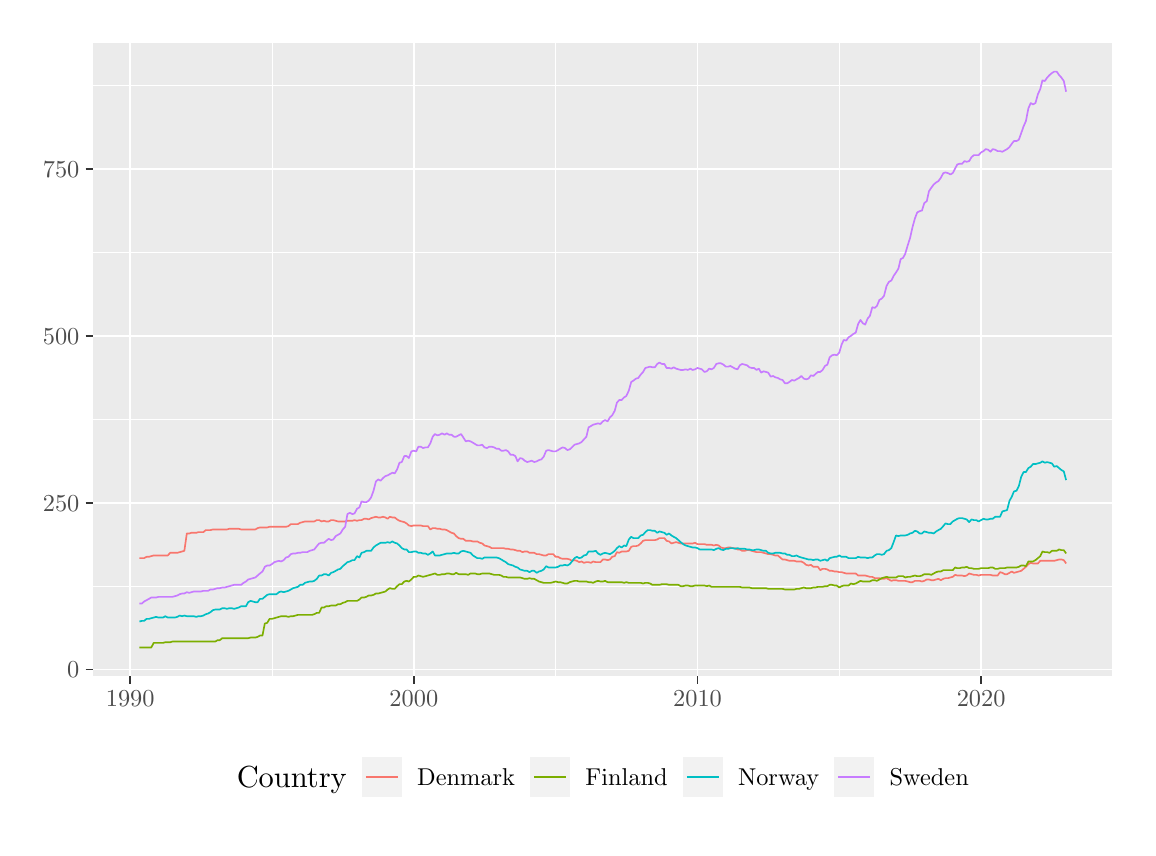
\begin{tikzpicture}[x=1pt,y=1pt]
\definecolor{fillColor}{RGB}{255,255,255}
\path[use as bounding box,fill=fillColor,fill opacity=0.00] (0,0) rectangle (397.48,289.08);
\begin{scope}
\path[clip] (  0.00,  0.00) rectangle (397.48,289.08);
\definecolor{drawColor}{RGB}{255,255,255}
\definecolor{fillColor}{RGB}{255,255,255}

\path[draw=drawColor,line width= 0.6pt,line join=round,line cap=round,fill=fillColor] (  0.00,  0.00) rectangle (397.48,289.08);
\end{scope}
\begin{scope}
\path[clip] ( 23.65, 54.68) rectangle (391.98,283.58);
\definecolor{fillColor}{gray}{0.92}

\path[fill=fillColor] ( 23.65, 54.68) rectangle (391.98,283.58);
\definecolor{drawColor}{RGB}{255,255,255}

\path[draw=drawColor,line width= 0.3pt,line join=round] ( 23.65, 87.26) --
	(391.98, 87.26);

\path[draw=drawColor,line width= 0.3pt,line join=round] ( 23.65,147.55) --
	(391.98,147.55);

\path[draw=drawColor,line width= 0.3pt,line join=round] ( 23.65,207.83) --
	(391.98,207.83);

\path[draw=drawColor,line width= 0.3pt,line join=round] ( 23.65,268.11) --
	(391.98,268.11);

\path[draw=drawColor,line width= 0.3pt,line join=round] ( 88.29, 54.68) --
	( 88.29,283.58);

\path[draw=drawColor,line width= 0.3pt,line join=round] (190.80, 54.68) --
	(190.80,283.58);

\path[draw=drawColor,line width= 0.3pt,line join=round] (293.30, 54.68) --
	(293.30,283.58);

\path[draw=drawColor,line width= 0.6pt,line join=round] ( 23.65, 57.12) --
	(391.98, 57.12);

\path[draw=drawColor,line width= 0.6pt,line join=round] ( 23.65,117.41) --
	(391.98,117.41);

\path[draw=drawColor,line width= 0.6pt,line join=round] ( 23.65,177.69) --
	(391.98,177.69);

\path[draw=drawColor,line width= 0.6pt,line join=round] ( 23.65,237.97) --
	(391.98,237.97);

\path[draw=drawColor,line width= 0.6pt,line join=round] ( 37.05, 54.68) --
	( 37.05,283.58);

\path[draw=drawColor,line width= 0.6pt,line join=round] (139.54, 54.68) --
	(139.54,283.58);

\path[draw=drawColor,line width= 0.6pt,line join=round] (242.05, 54.68) --
	(242.05,283.58);

\path[draw=drawColor,line width= 0.6pt,line join=round] (344.54, 54.68) --
	(344.54,283.58);
\definecolor{drawColor}{RGB}{248,118,109}

\path[draw=drawColor,line width= 0.6pt,line join=round] ( 40.39, 97.39) --
	( 41.26, 97.39) --
	( 42.07, 97.39) --
	( 42.97, 97.87) --
	( 43.84, 97.87) --
	( 44.63, 98.12) --
	( 45.55, 98.36) --
	( 46.40, 98.36) --
	( 47.27, 98.36) --
	( 48.13, 98.36) --
	( 48.92, 98.36) --
	( 49.73, 98.36) --
	( 50.63, 98.36) --
	( 51.50, 99.32) --
	( 52.29, 99.32) --
	( 53.21, 99.32) --
	( 54.06, 99.32) --
	( 54.93, 99.56) --
	( 55.80, 99.80) --
	( 56.61,100.04) --
	( 57.51,106.31) --
	( 58.38,106.31) --
	( 59.16,106.55) --
	( 60.06,106.55) --
	( 60.90,106.55) --
	( 61.72,106.80) --
	( 62.62,106.80) --
	( 63.49,106.80) --
	( 64.36,107.52) --
	( 65.20,107.52) --
	( 66.04,107.52) --
	( 66.91,107.76) --
	( 67.78,107.76) --
	( 68.59,107.76) --
	( 69.38,107.76) --
	( 70.31,107.76) --
	( 71.15,107.76) --
	( 72.02,107.76) --
	( 72.86,108.00) --
	( 73.70,108.00) --
	( 74.60,108.00) --
	( 75.44,108.00) --
	( 76.25,108.00) --
	( 77.15,107.76) --
	( 78.02,107.76) --
	( 78.89,107.76) --
	( 79.68,107.76) --
	( 80.55,107.76) --
	( 81.36,107.76) --
	( 82.26,107.76) --
	( 83.10,108.24) --
	( 83.92,108.48) --
	( 84.84,108.48) --
	( 85.68,108.48) --
	( 86.55,108.48) --
	( 87.40,108.72) --
	( 88.24,108.72) --
	( 89.14,108.72) --
	( 89.92,108.72) --
	( 90.79,108.72) --
	( 91.58,108.72) --
	( 92.50,108.72) --
	( 93.35,108.72) --
	( 94.22,108.97) --
	( 95.09,109.69) --
	( 95.90,109.69) --
	( 96.80,109.69) --
	( 97.64,109.69) --
	( 98.45,110.17) --
	( 99.38,110.41) --
	(100.19,110.65) --
	(101.01,110.65) --
	(101.90,110.65) --
	(102.77,110.65) --
	(103.56,110.65) --
	(104.49,111.14) --
	(105.33,111.14) --
	(106.20,110.65) --
	(107.07,110.89) --
	(107.88,110.65) --
	(108.78,110.65) --
	(109.65,111.14) --
	(110.44,111.14) --
	(111.31,110.89) --
	(112.15,110.65) --
	(112.99,110.65) --
	(113.86,110.65) --
	(114.73,110.65) --
	(115.54,110.89) --
	(116.44,110.89) --
	(117.31,110.89) --
	(118.10,111.14) --
	(119.02,110.89) --
	(119.87,111.14) --
	(120.65,111.14) --
	(121.55,111.62) --
	(122.39,111.62) --
	(123.20,111.38) --
	(124.10,111.86) --
	(124.97,112.10) --
	(125.84,112.34) --
	(126.68,112.10) --
	(127.53,112.10) --
	(128.40,112.34) --
	(129.27,112.10) --
	(130.08,111.62) --
	(130.87,112.34) --
	(131.79,112.10) --
	(132.63,112.10) --
	(133.50,111.38) --
	(134.35,110.89) --
	(135.19,110.65) --
	(136.09,110.41) --
	(136.93,109.93) --
	(137.74,109.21) --
	(138.64,108.97) --
	(139.51,109.21) --
	(140.38,109.21) --
	(141.19,109.21) --
	(142.06,109.21) --
	(142.85,108.97) --
	(143.78,108.97) --
	(144.62,108.97) --
	(145.49,107.76) --
	(146.36,108.24) --
	(147.17,108.24) --
	(148.07,108.00) --
	(148.91,108.00) --
	(149.72,107.76) --
	(150.65,107.76) --
	(151.44,107.52) --
	(152.28,107.04) --
	(153.15,106.55) --
	(154.02,106.31) --
	(154.83,105.35) --
	(155.73,104.63) --
	(156.60,104.38) --
	(157.39,104.38) --
	(158.31,103.66) --
	(159.15,103.66) --
	(160.02,103.66) --
	(160.89,103.42) --
	(161.68,103.42) --
	(162.49,103.42) --
	(163.39,102.94) --
	(164.26,102.70) --
	(165.05,101.97) --
	(165.97,101.73) --
	(166.82,101.49) --
	(167.69,101.01) --
	(168.56,101.01) --
	(169.37,101.01) --
	(170.27,101.01) --
	(171.14,101.01) --
	(171.92,101.01) --
	(172.79,100.77) --
	(173.63,100.77) --
	(174.48,100.53) --
	(175.35,100.53) --
	(176.22,100.29) --
	(177.03,100.04) --
	(177.93,100.04) --
	(178.80, 99.56) --
	(179.58, 99.80) --
	(180.51, 99.80) --
	(181.35, 99.32) --
	(182.14, 99.32) --
	(183.06, 99.32) --
	(183.91, 98.84) --
	(184.78, 98.84) --
	(185.62, 98.60) --
	(186.46, 98.36) --
	(187.36, 98.36) --
	(188.20, 98.84) --
	(189.01, 98.84) --
	(189.91, 98.84) --
	(190.78, 97.87) --
	(191.65, 97.87) --
	(192.44, 97.39) --
	(193.31, 97.15) --
	(194.12, 97.15) --
	(195.02, 97.15) --
	(195.86, 96.91) --
	(196.67, 96.43) --
	(197.60, 96.67) --
	(198.44, 96.43) --
	(199.31, 95.94) --
	(200.15, 96.19) --
	(201.00, 95.70) --
	(201.89, 95.94) --
	(202.68, 95.94) --
	(203.55, 95.70) --
	(204.34, 96.19) --
	(205.26, 95.94) --
	(206.10, 95.94) --
	(206.97, 95.94) --
	(207.84, 96.91) --
	(208.66, 96.91) --
	(209.56, 96.67) --
	(210.40, 96.91) --
	(211.21, 97.87) --
	(212.14, 98.12) --
	(212.92, 99.56) --
	(213.77, 99.32) --
	(214.64, 99.80) --
	(215.51, 99.80) --
	(216.32, 99.80) --
	(217.22,100.04) --
	(218.09,101.49) --
	(218.87,101.73) --
	(219.80,101.73) --
	(220.64,101.97) --
	(221.51,102.70) --
	(222.38,103.66) --
	(223.19,103.90) --
	(224.06,103.90) --
	(224.91,103.90) --
	(225.75,103.90) --
	(226.62,103.90) --
	(227.49,104.14) --
	(228.30,104.63) --
	(229.20,104.63) --
	(230.07,104.63) --
	(230.86,103.66) --
	(231.78,103.42) --
	(232.62,102.70) --
	(233.41,102.94) --
	(234.31,103.18) --
	(235.15,102.94) --
	(235.96,102.70) --
	(236.86,102.70) --
	(237.73,102.70) --
	(238.60,102.70) --
	(239.44,102.70) --
	(240.29,102.70) --
	(241.16,102.94) --
	(242.03,102.46) --
	(242.84,102.46) --
	(243.62,102.46) --
	(244.55,102.46) --
	(245.39,102.21) --
	(246.26,102.21) --
	(247.10,102.21) --
	(247.95,101.97) --
	(248.84,102.21) --
	(249.69,101.97) --
	(250.50,101.25) --
	(251.40,101.01) --
	(252.27,101.01) --
	(253.14,101.25) --
	(253.92,101.25) --
	(254.79,101.01) --
	(255.61,101.01) --
	(256.51,100.53) --
	(257.35,100.53) --
	(258.16,100.04) --
	(259.09,100.04) --
	(259.93,100.29) --
	(260.80,100.29) --
	(261.64,100.04) --
	(262.48, 99.80) --
	(263.38, 99.56) --
	(264.20, 99.56) --
	(265.04, 99.56) --
	(265.91, 99.32) --
	(266.78, 99.08) --
	(267.59, 98.84) --
	(268.49, 98.84) --
	(269.36, 98.60) --
	(270.14, 98.36) --
	(271.07, 98.36) --
	(271.91, 97.63) --
	(272.78, 96.91) --
	(273.65, 96.91) --
	(274.44, 96.67) --
	(275.25, 96.43) --
	(276.15, 96.43) --
	(277.02, 96.43) --
	(277.81, 96.19) --
	(278.73, 96.19) --
	(279.57, 96.19) --
	(280.44, 95.70) --
	(281.31, 94.98) --
	(282.13, 94.74) --
	(283.03, 94.98) --
	(283.90, 94.26) --
	(284.68, 94.26) --
	(285.55, 94.26) --
	(286.39, 93.05) --
	(287.24, 93.53) --
	(288.11, 93.53) --
	(288.98, 93.29) --
	(289.79, 92.81) --
	(290.69, 92.81) --
	(291.56, 92.57) --
	(292.34, 92.57) --
	(293.27, 92.33) --
	(294.11, 92.33) --
	(294.90, 92.09) --
	(295.79, 91.85) --
	(296.64, 91.85) --
	(297.45, 91.85) --
	(298.35, 91.85) --
	(299.22, 91.85) --
	(300.09, 91.12) --
	(300.93, 91.12) --
	(301.77, 91.12) --
	(302.64, 91.12) --
	(303.51, 90.88) --
	(304.33, 90.64) --
	(305.20, 90.64) --
	(306.07, 90.16) --
	(306.88, 90.16) --
	(307.78, 90.16) --
	(308.62, 89.92) --
	(309.43, 89.92) --
	(310.36, 90.16) --
	(311.20, 89.68) --
	(312.07, 89.19) --
	(312.91, 89.43) --
	(313.76, 89.43) --
	(314.65, 89.19) --
	(315.44, 89.19) --
	(316.31, 89.19) --
	(317.09, 89.19) --
	(318.02, 88.95) --
	(318.86, 88.71) --
	(319.73, 88.71) --
	(320.60, 89.19) --
	(321.42, 89.19) --
	(322.31, 89.19) --
	(323.16, 88.95) --
	(323.97, 89.19) --
	(324.90, 89.68) --
	(325.68, 89.68) --
	(326.52, 89.43) --
	(327.39, 89.43) --
	(328.26, 89.68) --
	(329.08, 89.92) --
	(329.98, 89.43) --
	(330.85, 89.92) --
	(331.63, 90.16) --
	(332.56, 90.16) --
	(333.40, 90.40) --
	(334.27, 90.64) --
	(335.14, 91.36) --
	(335.93, 91.12) --
	(336.74, 91.12) --
	(337.64, 91.12) --
	(338.51, 90.88) --
	(339.29, 91.12) --
	(340.22, 91.85) --
	(341.06, 91.60) --
	(341.93, 91.36) --
	(342.80, 91.36) --
	(343.61, 91.12) --
	(344.51, 91.36) --
	(345.38, 91.36) --
	(346.17, 91.36) --
	(347.07, 91.36) --
	(347.91, 91.36) --
	(348.72, 91.12) --
	(349.62, 91.12) --
	(350.49, 91.12) --
	(351.36, 92.33) --
	(352.20, 92.09) --
	(353.04, 91.60) --
	(353.91, 91.60) --
	(354.78, 92.09) --
	(355.60, 92.57) --
	(356.38, 92.09) --
	(357.31, 92.33) --
	(358.15, 92.57) --
	(359.02, 92.81) --
	(359.86, 93.53) --
	(360.71, 94.26) --
	(361.60, 95.22) --
	(362.45, 95.70) --
	(363.26, 95.46) --
	(364.16, 95.46) --
	(365.03, 95.46) --
	(365.90, 96.43) --
	(366.68, 96.43) --
	(367.55, 96.43) --
	(368.37, 96.43) --
	(369.26, 96.43) --
	(370.11, 96.43) --
	(370.92, 96.43) --
	(371.85, 96.67) --
	(372.69, 96.91) --
	(373.56, 96.91) --
	(374.40, 96.67) --
	(375.24, 95.46);
\definecolor{drawColor}{RGB}{124,174,0}

\path[draw=drawColor,line width= 0.6pt,line join=round] ( 40.39, 65.08) --
	( 41.26, 65.08) --
	( 42.07, 65.08) --
	( 42.97, 65.08) --
	( 43.84, 65.08) --
	( 44.63, 65.08) --
	( 45.55, 66.77) --
	( 46.40, 66.77) --
	( 47.27, 66.77) --
	( 48.13, 66.77) --
	( 48.92, 66.77) --
	( 49.73, 67.01) --
	( 50.63, 67.01) --
	( 51.50, 67.01) --
	( 52.29, 67.25) --
	( 53.21, 67.25) --
	( 54.06, 67.25) --
	( 54.93, 67.25) --
	( 55.80, 67.25) --
	( 56.61, 67.25) --
	( 57.51, 67.25) --
	( 58.38, 67.25) --
	( 59.16, 67.25) --
	( 60.06, 67.25) --
	( 60.90, 67.25) --
	( 61.72, 67.25) --
	( 62.62, 67.25) --
	( 63.49, 67.25) --
	( 64.36, 67.25) --
	( 65.20, 67.25) --
	( 66.04, 67.25) --
	( 66.91, 67.25) --
	( 67.78, 67.25) --
	( 68.59, 67.73) --
	( 69.38, 67.73) --
	( 70.31, 68.46) --
	( 71.15, 68.46) --
	( 72.02, 68.46) --
	( 72.86, 68.46) --
	( 73.70, 68.46) --
	( 74.60, 68.46) --
	( 75.44, 68.46) --
	( 76.25, 68.46) --
	( 77.15, 68.46) --
	( 78.02, 68.46) --
	( 78.89, 68.46) --
	( 79.68, 68.46) --
	( 80.55, 68.70) --
	( 81.36, 68.70) --
	( 82.26, 68.70) --
	( 83.10, 68.94) --
	( 83.92, 69.42) --
	( 84.84, 69.42) --
	( 85.68, 73.76) --
	( 86.55, 74.00) --
	( 87.40, 75.45) --
	( 88.24, 75.45) --
	( 89.14, 75.69) --
	( 89.92, 75.93) --
	( 90.79, 76.17) --
	( 91.58, 76.41) --
	( 92.50, 76.41) --
	( 93.35, 76.41) --
	( 94.22, 76.17) --
	( 95.09, 76.41) --
	( 95.90, 76.41) --
	( 96.80, 76.65) --
	( 97.64, 76.90) --
	( 98.45, 76.90) --
	( 99.38, 76.90) --
	(100.19, 76.90) --
	(101.01, 76.90) --
	(101.90, 76.90) --
	(102.77, 76.90) --
	(103.56, 77.14) --
	(104.49, 77.62) --
	(105.33, 77.62) --
	(106.20, 79.55) --
	(107.07, 79.55) --
	(107.88, 80.03) --
	(108.78, 80.03) --
	(109.65, 80.27) --
	(110.44, 80.27) --
	(111.31, 80.27) --
	(112.15, 80.75) --
	(112.99, 80.75) --
	(113.86, 81.24) --
	(114.73, 81.48) --
	(115.54, 81.96) --
	(116.44, 81.96) --
	(117.31, 81.96) --
	(118.10, 81.96) --
	(119.02, 81.96) --
	(119.87, 82.44) --
	(120.65, 83.16) --
	(121.55, 83.16) --
	(122.39, 83.41) --
	(123.20, 83.89) --
	(124.10, 83.89) --
	(124.97, 84.13) --
	(125.84, 84.61) --
	(126.68, 84.61) --
	(127.53, 84.85) --
	(128.40, 85.09) --
	(129.27, 85.34) --
	(130.08, 86.06) --
	(130.87, 86.54) --
	(131.79, 86.30) --
	(132.63, 86.30) --
	(133.50, 87.26) --
	(134.35, 87.99) --
	(135.19, 87.99) --
	(136.09, 88.95) --
	(136.93, 89.19) --
	(137.74, 88.95) --
	(138.64, 89.68) --
	(139.51, 90.64) --
	(140.38, 90.64) --
	(141.19, 91.12) --
	(142.06, 90.88) --
	(142.85, 90.64) --
	(143.78, 90.88) --
	(144.62, 91.12) --
	(145.49, 91.36) --
	(146.36, 91.60) --
	(147.17, 91.85) --
	(148.07, 91.36) --
	(148.91, 91.36) --
	(149.72, 91.60) --
	(150.65, 91.60) --
	(151.44, 91.85) --
	(152.28, 91.85) --
	(153.15, 91.60) --
	(154.02, 91.60) --
	(154.83, 92.09) --
	(155.73, 91.60) --
	(156.60, 91.60) --
	(157.39, 91.60) --
	(158.31, 91.60) --
	(159.15, 91.36) --
	(160.02, 91.85) --
	(160.89, 91.85) --
	(161.68, 91.85) --
	(162.49, 91.60) --
	(163.39, 91.60) --
	(164.26, 91.85) --
	(165.05, 91.85) --
	(165.97, 91.85) --
	(166.82, 91.85) --
	(167.69, 91.60) --
	(168.56, 91.36) --
	(169.37, 91.36) --
	(170.27, 91.36) --
	(171.14, 91.12) --
	(171.92, 90.64) --
	(172.79, 90.64) --
	(173.63, 90.40) --
	(174.48, 90.40) --
	(175.35, 90.40) --
	(176.22, 90.40) --
	(177.03, 90.40) --
	(177.93, 90.40) --
	(178.80, 90.16) --
	(179.58, 89.92) --
	(180.51, 89.92) --
	(181.35, 90.16) --
	(182.14, 89.92) --
	(183.06, 89.92) --
	(183.91, 89.43) --
	(184.78, 88.95) --
	(185.62, 88.71) --
	(186.46, 88.47) --
	(187.36, 88.47) --
	(188.20, 88.47) --
	(189.01, 88.47) --
	(189.91, 88.71) --
	(190.78, 88.95) --
	(191.65, 88.71) --
	(192.44, 88.71) --
	(193.31, 88.47) --
	(194.12, 88.23) --
	(195.02, 88.23) --
	(195.86, 88.71) --
	(196.67, 88.95) --
	(197.60, 89.19) --
	(198.44, 89.19) --
	(199.31, 88.95) --
	(200.15, 88.95) --
	(201.00, 88.95) --
	(201.89, 88.95) --
	(202.68, 88.71) --
	(203.55, 88.71) --
	(204.34, 88.47) --
	(205.26, 88.95) --
	(206.10, 89.19) --
	(206.97, 88.95) --
	(207.84, 88.95) --
	(208.66, 89.19) --
	(209.56, 88.71) --
	(210.40, 88.71) --
	(211.21, 88.71) --
	(212.14, 88.71) --
	(212.92, 88.71) --
	(213.77, 88.71) --
	(214.64, 88.71) --
	(215.51, 88.47) --
	(216.32, 88.71) --
	(217.22, 88.47) --
	(218.09, 88.47) --
	(218.87, 88.47) --
	(219.80, 88.47) --
	(220.64, 88.47) --
	(221.51, 88.47) --
	(222.38, 88.23) --
	(223.19, 88.47) --
	(224.06, 88.47) --
	(224.91, 88.23) --
	(225.75, 87.75) --
	(226.62, 87.75) --
	(227.49, 87.75) --
	(228.30, 87.75) --
	(229.20, 87.99) --
	(230.07, 87.99) --
	(230.86, 87.99) --
	(231.78, 87.75) --
	(232.62, 87.75) --
	(233.41, 87.75) --
	(234.31, 87.75) --
	(235.15, 87.75) --
	(235.96, 87.26) --
	(236.86, 87.26) --
	(237.73, 87.51) --
	(238.60, 87.51) --
	(239.44, 87.26) --
	(240.29, 87.26) --
	(241.16, 87.51) --
	(242.03, 87.51) --
	(242.84, 87.51) --
	(243.62, 87.51) --
	(244.55, 87.51) --
	(245.39, 87.26) --
	(246.26, 87.51) --
	(247.10, 87.02) --
	(247.95, 87.02) --
	(248.84, 87.02) --
	(249.69, 87.02) --
	(250.50, 87.02) --
	(251.40, 87.02) --
	(252.27, 87.02) --
	(253.14, 87.02) --
	(253.92, 87.02) --
	(254.79, 87.02) --
	(255.61, 87.02) --
	(256.51, 87.02) --
	(257.35, 87.02) --
	(258.16, 86.78) --
	(259.09, 86.78) --
	(259.93, 86.78) --
	(260.80, 86.78) --
	(261.64, 86.54) --
	(262.48, 86.54) --
	(263.38, 86.54) --
	(264.20, 86.54) --
	(265.04, 86.54) --
	(265.91, 86.54) --
	(266.78, 86.54) --
	(267.59, 86.30) --
	(268.49, 86.30) --
	(269.36, 86.30) --
	(270.14, 86.30) --
	(271.07, 86.30) --
	(271.91, 86.30) --
	(272.78, 86.30) --
	(273.65, 86.06) --
	(274.44, 86.06) --
	(275.25, 86.06) --
	(276.15, 86.06) --
	(277.02, 86.06) --
	(277.81, 86.30) --
	(278.73, 86.30) --
	(279.57, 86.54) --
	(280.44, 86.78) --
	(281.31, 86.54) --
	(282.13, 86.54) --
	(283.03, 86.54) --
	(283.90, 86.78) --
	(284.68, 86.78) --
	(285.55, 87.02) --
	(286.39, 87.02) --
	(287.24, 87.02) --
	(288.11, 87.26) --
	(288.98, 87.26) --
	(289.79, 87.75) --
	(290.69, 87.75) --
	(291.56, 87.51) --
	(292.34, 87.51) --
	(293.27, 86.78) --
	(294.11, 87.26) --
	(294.90, 87.51) --
	(295.79, 87.51) --
	(296.64, 87.51) --
	(297.45, 88.23) --
	(298.35, 87.99) --
	(299.22, 88.23) --
	(300.09, 88.71) --
	(300.93, 89.19) --
	(301.77, 88.95) --
	(302.64, 88.95) --
	(303.51, 88.95) --
	(304.33, 88.95) --
	(305.20, 89.43) --
	(306.07, 89.43) --
	(306.88, 89.19) --
	(307.78, 89.68) --
	(308.62, 90.16) --
	(309.43, 90.40) --
	(310.36, 90.64) --
	(311.20, 90.40) --
	(312.07, 90.40) --
	(312.91, 90.40) --
	(313.76, 90.40) --
	(314.65, 90.88) --
	(315.44, 90.88) --
	(316.31, 90.88) --
	(317.09, 90.40) --
	(318.02, 90.64) --
	(318.86, 90.64) --
	(319.73, 90.88) --
	(320.60, 91.12) --
	(321.42, 90.88) --
	(322.31, 90.88) --
	(323.16, 91.12) --
	(323.97, 91.60) --
	(324.90, 91.60) --
	(325.68, 91.60) --
	(326.52, 91.36) --
	(327.39, 91.85) --
	(328.26, 92.33) --
	(329.08, 92.57) --
	(329.98, 92.57) --
	(330.85, 93.05) --
	(331.63, 93.05) --
	(332.56, 93.05) --
	(333.40, 93.05) --
	(334.27, 93.05) --
	(335.14, 94.02) --
	(335.93, 93.77) --
	(336.74, 93.77) --
	(337.64, 94.02) --
	(338.51, 94.02) --
	(339.29, 94.26) --
	(340.22, 93.77) --
	(341.06, 93.77) --
	(341.93, 93.53) --
	(342.80, 93.53) --
	(343.61, 93.53) --
	(344.51, 93.77) --
	(345.38, 93.77) --
	(346.17, 93.77) --
	(347.07, 93.77) --
	(347.91, 94.02) --
	(348.72, 94.02) --
	(349.62, 93.53) --
	(350.49, 93.53) --
	(351.36, 93.77) --
	(352.20, 93.77) --
	(353.04, 93.77) --
	(353.91, 94.02) --
	(354.78, 94.02) --
	(355.60, 94.02) --
	(356.38, 94.02) --
	(357.31, 94.02) --
	(358.15, 94.26) --
	(359.02, 94.74) --
	(359.86, 94.74) --
	(360.71, 94.50) --
	(361.60, 96.19) --
	(362.45, 96.19) --
	(363.26, 96.19) --
	(364.16, 96.67) --
	(365.03, 97.39) --
	(365.90, 98.12) --
	(366.68, 99.80) --
	(367.55, 99.56) --
	(368.37, 99.56) --
	(369.26, 99.32) --
	(370.11,100.04) --
	(370.92,100.04) --
	(371.85,100.04) --
	(372.69,100.53) --
	(373.56,100.29) --
	(374.40,100.29) --
	(375.24, 99.08);
\definecolor{drawColor}{RGB}{0,191,196}

\path[draw=drawColor,line width= 0.6pt,line join=round] ( 40.39, 74.48) --
	( 41.26, 74.73) --
	( 42.07, 74.73) --
	( 42.97, 75.45) --
	( 43.84, 75.45) --
	( 44.63, 75.69) --
	( 45.55, 75.93) --
	( 46.40, 76.17) --
	( 47.27, 75.93) --
	( 48.13, 75.93) --
	( 48.92, 75.93) --
	( 49.73, 76.41) --
	( 50.63, 75.93) --
	( 51.50, 75.93) --
	( 52.29, 75.93) --
	( 53.21, 75.93) --
	( 54.06, 76.17) --
	( 54.93, 76.65) --
	( 55.80, 76.41) --
	( 56.61, 76.65) --
	( 57.51, 76.41) --
	( 58.38, 76.41) --
	( 59.16, 76.41) --
	( 60.06, 76.41) --
	( 60.90, 76.17) --
	( 61.72, 76.41) --
	( 62.62, 76.41) --
	( 63.49, 76.65) --
	( 64.36, 77.14) --
	( 65.20, 77.38) --
	( 66.04, 77.86) --
	( 66.91, 78.58) --
	( 67.78, 78.82) --
	( 68.59, 78.82) --
	( 69.38, 78.82) --
	( 70.31, 79.31) --
	( 71.15, 79.31) --
	( 72.02, 79.07) --
	( 72.86, 79.31) --
	( 73.70, 79.31) --
	( 74.60, 79.07) --
	( 75.44, 79.31) --
	( 76.25, 79.55) --
	( 77.15, 80.03) --
	( 78.02, 80.03) --
	( 78.89, 80.03) --
	( 79.68, 81.48) --
	( 80.55, 81.96) --
	( 81.36, 81.72) --
	( 82.26, 81.48) --
	( 83.10, 81.48) --
	( 83.92, 82.68) --
	( 84.84, 82.68) --
	( 85.68, 83.41) --
	( 86.55, 84.13) --
	( 87.40, 84.37) --
	( 88.24, 84.37) --
	( 89.14, 84.37) --
	( 89.92, 84.37) --
	( 90.79, 85.09) --
	( 91.58, 85.34) --
	( 92.50, 85.09) --
	( 93.35, 85.34) --
	( 94.22, 85.58) --
	( 95.09, 86.06) --
	( 95.90, 86.54) --
	( 96.80, 86.78) --
	( 97.64, 87.02) --
	( 98.45, 87.75) --
	( 99.38, 87.75) --
	(100.19, 88.47) --
	(101.01, 88.71) --
	(101.90, 88.95) --
	(102.77, 88.95) --
	(103.56, 89.19) --
	(104.49, 89.92) --
	(105.33, 91.12) --
	(106.20, 91.12) --
	(107.07, 91.60) --
	(107.88, 91.60) --
	(108.78, 91.12) --
	(109.65, 92.09) --
	(110.44, 92.33) --
	(111.31, 92.81) --
	(112.15, 93.29) --
	(112.99, 93.53) --
	(113.86, 94.50) --
	(114.73, 95.22) --
	(115.54, 95.94) --
	(116.44, 96.19) --
	(117.31, 96.67) --
	(118.10, 96.67) --
	(119.02, 98.12) --
	(119.87, 97.63) --
	(120.65, 99.32) --
	(121.55, 99.56) --
	(122.39,100.04) --
	(123.20,100.04) --
	(124.10,100.04) --
	(124.97,101.25) --
	(125.84,101.97) --
	(126.68,102.46) --
	(127.53,102.94) --
	(128.40,102.94) --
	(129.27,102.94) --
	(130.08,103.18) --
	(130.87,102.94) --
	(131.79,103.42) --
	(132.63,102.94) --
	(133.50,102.70) --
	(134.35,101.97) --
	(135.19,101.01) --
	(136.09,100.53) --
	(136.93,100.53) --
	(137.74, 99.56) --
	(138.64, 99.56) --
	(139.51, 99.80) --
	(140.38, 99.80) --
	(141.19, 99.32) --
	(142.06, 99.32) --
	(142.85, 99.08) --
	(143.78, 99.08) --
	(144.62, 98.60) --
	(145.49, 99.08) --
	(146.36, 99.80) --
	(147.17, 98.36) --
	(148.07, 98.36) --
	(148.91, 98.36) --
	(149.72, 98.60) --
	(150.65, 98.84) --
	(151.44, 99.08) --
	(152.28, 99.08) --
	(153.15, 99.08) --
	(154.02, 99.32) --
	(154.83, 99.08) --
	(155.73, 99.08) --
	(156.60, 99.80) --
	(157.39,100.04) --
	(158.31, 99.80) --
	(159.15, 99.56) --
	(160.02, 99.32) --
	(160.89, 98.36) --
	(161.68, 97.87) --
	(162.49, 97.39) --
	(163.39, 97.39) --
	(164.26, 97.15) --
	(165.05, 97.63) --
	(165.97, 97.63) --
	(166.82, 97.63) --
	(167.69, 97.63) --
	(168.56, 97.63) --
	(169.37, 97.63) --
	(170.27, 97.39) --
	(171.14, 96.91) --
	(171.92, 96.43) --
	(172.79, 95.94) --
	(173.63, 95.22) --
	(174.48, 94.98) --
	(175.35, 94.74) --
	(176.22, 94.26) --
	(177.03, 94.02) --
	(177.93, 93.29) --
	(178.80, 93.05) --
	(179.58, 92.81) --
	(180.51, 92.81) --
	(181.35, 92.33) --
	(182.14, 92.81) --
	(183.06, 92.81) --
	(183.91, 92.09) --
	(184.78, 92.57) --
	(185.62, 92.81) --
	(186.46, 93.29) --
	(187.36, 94.50) --
	(188.20, 94.02) --
	(189.01, 94.02) --
	(189.91, 94.02) --
	(190.78, 94.02) --
	(191.65, 94.26) --
	(192.44, 94.74) --
	(193.31, 94.74) --
	(194.12, 94.98) --
	(195.02, 94.74) --
	(195.86, 95.22) --
	(196.67, 96.19) --
	(197.60, 97.39) --
	(198.44, 97.87) --
	(199.31, 97.39) --
	(200.15, 97.63) --
	(201.00, 98.36) --
	(201.89, 98.60) --
	(202.68, 99.80) --
	(203.55, 99.80) --
	(204.34, 99.80) --
	(205.26,100.04) --
	(206.10, 99.08) --
	(206.97, 98.60) --
	(207.84, 99.08) --
	(208.66, 99.32) --
	(209.56, 99.08) --
	(210.40, 98.84) --
	(211.21, 99.32) --
	(212.14,100.04) --
	(212.92,101.01) --
	(213.77,101.73) --
	(214.64,101.25) --
	(215.51,101.97) --
	(216.32,101.73) --
	(217.22,104.14) --
	(218.09,105.11) --
	(218.87,104.63) --
	(219.80,104.63) --
	(220.64,104.63) --
	(221.51,105.59) --
	(222.38,105.83) --
	(223.19,106.80) --
	(224.06,107.52) --
	(224.91,107.52) --
	(225.75,107.28) --
	(226.62,107.28) --
	(227.49,106.55) --
	(228.30,107.04) --
	(229.20,106.80) --
	(230.07,106.55) --
	(230.86,105.83) --
	(231.78,106.31) --
	(232.62,105.59) --
	(233.41,105.11) --
	(234.31,104.63) --
	(235.15,103.90) --
	(235.96,103.18) --
	(236.86,102.46) --
	(237.73,101.97) --
	(238.60,101.73) --
	(239.44,101.49) --
	(240.29,101.25) --
	(241.16,101.25) --
	(242.03,101.01) --
	(242.84,100.53) --
	(243.62,100.53) --
	(244.55,100.53) --
	(245.39,100.53) --
	(246.26,100.53) --
	(247.10,100.53) --
	(247.95,100.29) --
	(248.84,100.77) --
	(249.69,101.01) --
	(250.50,100.53) --
	(251.40,100.29) --
	(252.27,100.77) --
	(253.14,100.77) --
	(253.92,101.01) --
	(254.79,101.01) --
	(255.61,100.77) --
	(256.51,101.01) --
	(257.35,100.77) --
	(258.16,100.77) --
	(259.09,100.77) --
	(259.93,100.53) --
	(260.80,100.53) --
	(261.64,100.29) --
	(262.48,100.29) --
	(263.38,100.53) --
	(264.20,100.53) --
	(265.04,100.29) --
	(265.91,100.04) --
	(266.78,100.04) --
	(267.59, 99.32) --
	(268.49, 99.08) --
	(269.36, 99.08) --
	(270.14, 99.32) --
	(271.07, 99.32) --
	(271.91, 99.32) --
	(272.78, 99.08) --
	(273.65, 99.08) --
	(274.44, 98.60) --
	(275.25, 98.60) --
	(276.15, 98.12) --
	(277.02, 98.12) --
	(277.81, 98.36) --
	(278.73, 97.87) --
	(279.57, 97.63) --
	(280.44, 97.39) --
	(281.31, 97.15) --
	(282.13, 96.91) --
	(283.03, 96.91) --
	(283.90, 96.67) --
	(284.68, 96.91) --
	(285.55, 96.91) --
	(286.39, 96.43) --
	(287.24, 96.67) --
	(288.11, 96.91) --
	(288.98, 96.43) --
	(289.79, 97.39) --
	(290.69, 97.63) --
	(291.56, 97.87) --
	(292.34, 97.87) --
	(293.27, 98.36) --
	(294.11, 97.87) --
	(294.90, 97.87) --
	(295.79, 97.87) --
	(296.64, 97.39) --
	(297.45, 97.39) --
	(298.35, 97.39) --
	(299.22, 97.39) --
	(300.09, 97.87) --
	(300.93, 97.63) --
	(301.77, 97.63) --
	(302.64, 97.63) --
	(303.51, 97.39) --
	(304.33, 97.63) --
	(305.20, 97.63) --
	(306.07, 98.36) --
	(306.88, 98.84) --
	(307.78, 98.84) --
	(308.62, 98.60) --
	(309.43, 98.84) --
	(310.36,100.04) --
	(311.20,100.29) --
	(312.07,101.01) --
	(312.91,103.18) --
	(313.76,105.59) --
	(314.65,105.35) --
	(315.44,105.59) --
	(316.31,105.59) --
	(317.09,105.59) --
	(318.02,105.83) --
	(318.86,106.31) --
	(319.73,106.55) --
	(320.60,107.28) --
	(321.42,107.04) --
	(322.31,106.31) --
	(323.16,106.31) --
	(323.97,107.04) --
	(324.90,106.80) --
	(325.68,106.55) --
	(326.52,106.55) --
	(327.39,106.31) --
	(328.26,107.04) --
	(329.08,107.52) --
	(329.98,108.00) --
	(330.85,108.97) --
	(331.63,109.93) --
	(332.56,109.69) --
	(333.40,109.69) --
	(334.27,110.65) --
	(335.14,111.14) --
	(335.93,111.62) --
	(336.74,111.86) --
	(337.64,111.86) --
	(338.51,111.62) --
	(339.29,111.38) --
	(340.22,110.41) --
	(341.06,111.38) --
	(341.93,111.14) --
	(342.80,111.14) --
	(343.61,110.65) --
	(344.51,111.14) --
	(345.38,111.62) --
	(346.17,111.38) --
	(347.07,111.38) --
	(347.91,111.62) --
	(348.72,111.62) --
	(349.62,112.34) --
	(350.49,112.34) --
	(351.36,112.34) --
	(352.20,114.27) --
	(353.04,114.51) --
	(353.91,114.75) --
	(354.78,118.13) --
	(355.60,119.58) --
	(356.38,121.50) --
	(357.31,121.75) --
	(358.15,123.43) --
	(359.02,126.81) --
	(359.86,128.50) --
	(360.71,128.50) --
	(361.60,129.94) --
	(362.45,130.43) --
	(363.26,131.39) --
	(364.16,131.39) --
	(365.03,131.63) --
	(365.90,131.87) --
	(366.68,132.36) --
	(367.55,131.87) --
	(368.37,132.11) --
	(369.26,131.87) --
	(370.11,131.63) --
	(370.92,130.43) --
	(371.85,130.67) --
	(372.69,129.94) --
	(373.56,129.22) --
	(374.40,128.74) --
	(375.24,125.60);
\definecolor{drawColor}{RGB}{199,124,255}

\path[draw=drawColor,line width= 0.6pt,line join=round] ( 40.39, 80.99) --
	( 41.26, 80.99) --
	( 42.07, 81.72) --
	( 42.97, 82.20) --
	( 43.84, 82.68) --
	( 44.63, 83.16) --
	( 45.55, 83.16) --
	( 46.40, 83.16) --
	( 47.27, 83.41) --
	( 48.13, 83.41) --
	( 48.92, 83.41) --
	( 49.73, 83.41) --
	( 50.63, 83.41) --
	( 51.50, 83.41) --
	( 52.29, 83.41) --
	( 53.21, 83.65) --
	( 54.06, 83.89) --
	( 54.93, 84.37) --
	( 55.80, 84.61) --
	( 56.61, 84.61) --
	( 57.51, 85.09) --
	( 58.38, 84.85) --
	( 59.16, 85.09) --
	( 60.06, 85.34) --
	( 60.90, 85.34) --
	( 61.72, 85.34) --
	( 62.62, 85.34) --
	( 63.49, 85.58) --
	( 64.36, 85.58) --
	( 65.20, 85.58) --
	( 66.04, 86.06) --
	( 66.91, 86.06) --
	( 67.78, 86.30) --
	( 68.59, 86.54) --
	( 69.38, 86.54) --
	( 70.31, 86.78) --
	( 71.15, 86.78) --
	( 72.02, 87.02) --
	( 72.86, 87.26) --
	( 73.70, 87.51) --
	( 74.60, 87.75) --
	( 75.44, 87.75) --
	( 76.25, 87.75) --
	( 77.15, 87.75) --
	( 78.02, 88.47) --
	( 78.89, 88.95) --
	( 79.68, 89.68) --
	( 80.55, 89.92) --
	( 81.36, 90.16) --
	( 82.26, 90.40) --
	( 83.10, 91.12) --
	( 83.92, 91.85) --
	( 84.84, 92.57) --
	( 85.68, 94.26) --
	( 86.55, 94.74) --
	( 87.40, 94.74) --
	( 88.24, 95.22) --
	( 89.14, 95.94) --
	( 89.92, 96.19) --
	( 90.79, 96.43) --
	( 91.58, 96.19) --
	( 92.50, 96.67) --
	( 93.35, 97.63) --
	( 94.22, 97.87) --
	( 95.09, 98.84) --
	( 95.90, 99.08) --
	( 96.80, 99.08) --
	( 97.64, 99.32) --
	( 98.45, 99.32) --
	( 99.38, 99.56) --
	(100.19, 99.56) --
	(101.01, 99.56) --
	(101.90,100.04) --
	(102.77,100.29) --
	(103.56,100.53) --
	(104.49,101.73) --
	(105.33,102.70) --
	(106.20,102.94) --
	(107.07,102.94) --
	(107.88,103.66) --
	(108.78,104.38) --
	(109.65,103.90) --
	(110.44,104.14) --
	(111.31,105.35) --
	(112.15,105.83) --
	(112.99,106.31) --
	(113.86,107.76) --
	(114.73,108.72) --
	(115.54,113.31) --
	(116.44,113.79) --
	(117.31,113.31) --
	(118.10,113.55) --
	(119.02,115.24) --
	(119.87,115.72) --
	(120.65,117.89) --
	(121.55,117.65) --
	(122.39,117.65) --
	(123.20,118.13) --
	(124.10,119.33) --
	(124.97,121.75) --
	(125.84,125.12) --
	(126.68,125.84) --
	(127.53,125.36) --
	(128.40,126.33) --
	(129.27,127.05) --
	(130.08,127.29) --
	(130.87,127.77) --
	(131.79,128.26) --
	(132.63,128.02) --
	(133.50,129.46) --
	(134.35,131.87) --
	(135.19,132.11) --
	(136.09,134.28) --
	(136.93,134.28) --
	(137.74,133.56) --
	(138.64,135.97) --
	(139.51,136.21) --
	(140.38,135.97) --
	(141.19,137.66) --
	(142.06,137.66) --
	(142.85,137.18) --
	(143.78,137.42) --
	(144.62,137.42) --
	(145.49,138.87) --
	(146.36,141.28) --
	(147.17,142.24) --
	(148.07,141.76) --
	(148.91,142.00) --
	(149.72,142.48) --
	(150.65,142.00) --
	(151.44,142.48) --
	(152.28,142.00) --
	(153.15,142.00) --
	(154.02,141.28) --
	(154.83,141.28) --
	(155.73,141.76) --
	(156.60,142.24) --
	(157.39,141.04) --
	(158.31,139.59) --
	(159.15,139.83) --
	(160.02,139.59) --
	(160.89,139.11) --
	(161.68,138.62) --
	(162.49,138.14) --
	(163.39,138.14) --
	(164.26,138.38) --
	(165.05,137.42) --
	(165.97,137.18) --
	(166.82,137.66) --
	(167.69,137.66) --
	(168.56,137.42) --
	(169.37,136.94) --
	(170.27,136.94) --
	(171.14,136.21) --
	(171.92,136.21) --
	(172.79,136.45) --
	(173.63,135.97) --
	(174.48,134.77) --
	(175.35,134.77) --
	(176.22,134.28) --
	(177.03,132.36) --
	(177.93,133.56) --
	(178.80,133.32) --
	(179.58,132.60) --
	(180.51,132.11) --
	(181.35,132.36) --
	(182.14,132.60) --
	(183.06,132.11) --
	(183.91,132.36) --
	(184.78,132.84) --
	(185.62,133.08) --
	(186.46,134.04) --
	(187.36,136.21) --
	(188.20,136.45) --
	(189.01,136.21) --
	(189.91,135.97) --
	(190.78,135.97) --
	(191.65,136.45) --
	(192.44,136.94) --
	(193.31,137.42) --
	(194.12,137.18) --
	(195.02,136.45) --
	(195.86,136.70) --
	(196.67,137.42) --
	(197.60,138.38) --
	(198.44,138.62) --
	(199.31,138.87) --
	(200.15,139.35) --
	(201.00,140.31) --
	(201.89,141.28) --
	(202.68,144.65) --
	(203.55,145.14) --
	(204.34,145.62) --
	(205.26,145.86) --
	(206.10,146.10) --
	(206.97,145.86) --
	(207.84,146.82) --
	(208.66,147.31) --
	(209.56,146.82) --
	(210.40,148.27) --
	(211.21,148.99) --
	(212.14,150.68) --
	(212.92,153.57) --
	(213.77,154.54) --
	(214.64,154.54) --
	(215.51,155.50) --
	(216.32,155.99) --
	(217.22,157.92) --
	(218.09,161.05) --
	(218.87,161.53) --
	(219.80,162.26) --
	(220.64,162.50) --
	(221.51,163.70) --
	(222.38,164.67) --
	(223.19,166.11) --
	(224.06,166.35) --
	(224.91,166.60) --
	(225.75,166.35) --
	(226.62,166.35) --
	(227.49,167.56) --
	(228.30,168.04) --
	(229.20,167.56) --
	(230.07,167.56) --
	(230.86,166.11) --
	(231.78,166.11) --
	(232.62,165.87) --
	(233.41,166.35) --
	(234.31,165.87) --
	(235.15,165.63) --
	(235.96,165.39) --
	(236.86,165.39) --
	(237.73,165.63) --
	(238.60,165.39) --
	(239.44,165.87) --
	(240.29,165.39) --
	(241.16,165.63) --
	(242.03,166.11) --
	(242.84,165.87) --
	(243.62,165.63) --
	(244.55,164.67) --
	(245.39,164.91) --
	(246.26,165.87) --
	(247.10,165.63) --
	(247.95,166.11) --
	(248.84,167.56) --
	(249.69,167.80) --
	(250.50,167.80) --
	(251.40,167.32) --
	(252.27,166.60) --
	(253.14,166.60) --
	(253.92,166.84) --
	(254.79,166.35) --
	(255.61,165.87) --
	(256.51,165.63) --
	(257.35,167.08) --
	(258.16,167.56) --
	(259.09,167.32) --
	(259.93,167.08) --
	(260.80,166.35) --
	(261.64,166.11) --
	(262.48,166.11) --
	(263.38,165.39) --
	(264.20,165.87) --
	(265.04,164.43) --
	(265.91,164.91) --
	(266.78,164.67) --
	(267.59,164.43) --
	(268.49,162.98) --
	(269.36,163.22) --
	(270.14,162.74) --
	(271.07,162.50) --
	(271.91,162.01) --
	(272.78,161.77) --
	(273.65,160.57) --
	(274.44,160.57) --
	(275.25,161.05) --
	(276.15,161.77) --
	(277.02,161.53) --
	(277.81,162.01) --
	(278.73,162.50) --
	(279.57,163.22) --
	(280.44,162.26) --
	(281.31,162.01) --
	(282.13,162.26) --
	(283.03,163.46) --
	(283.90,163.22) --
	(284.68,163.94) --
	(285.55,164.67) --
	(286.39,164.67) --
	(287.24,165.39) --
	(288.11,166.84) --
	(288.98,167.32) --
	(289.79,169.97) --
	(290.69,170.70) --
	(291.56,170.94) --
	(292.34,170.70) --
	(293.27,171.66) --
	(294.11,174.55) --
	(294.90,176.24) --
	(295.79,176.00) --
	(296.64,177.21) --
	(297.45,177.69) --
	(298.35,178.41) --
	(299.22,178.89) --
	(300.09,182.03) --
	(300.93,183.47) --
	(301.77,182.27) --
	(302.64,181.79) --
	(303.51,183.96) --
	(304.33,184.92) --
	(305.20,188.06) --
	(306.07,187.82) --
	(306.88,188.54) --
	(307.78,190.71) --
	(308.62,191.19) --
	(309.43,192.16) --
	(310.36,195.77) --
	(311.20,197.22) --
	(312.07,197.70) --
	(312.91,199.39) --
	(313.76,200.60) --
	(314.65,202.04) --
	(315.44,205.42) --
	(316.31,205.90) --
	(317.09,207.35) --
	(318.02,210.48) --
	(318.86,213.13) --
	(319.73,216.99) --
	(320.60,220.13) --
	(321.42,222.30) --
	(322.31,222.78) --
	(323.16,223.02) --
	(323.97,225.67) --
	(324.90,226.40) --
	(325.68,230.01) --
	(326.52,231.22) --
	(327.39,232.42) --
	(328.26,233.15) --
	(329.08,233.63) --
	(329.98,234.84) --
	(330.85,236.52) --
	(331.63,236.76) --
	(332.56,236.52) --
	(333.40,236.04) --
	(334.27,236.52) --
	(335.14,238.21) --
	(335.93,239.66) --
	(336.74,239.90) --
	(337.64,239.90) --
	(338.51,240.86) --
	(339.29,240.62) --
	(340.22,240.86) --
	(341.06,242.31) --
	(341.93,243.03) --
	(342.80,243.03) --
	(343.61,243.03) --
	(344.51,244.00) --
	(345.38,244.48) --
	(346.17,245.20) --
	(347.07,244.96) --
	(347.91,244.24) --
	(348.72,245.20) --
	(349.62,244.96) --
	(350.49,244.48) --
	(351.36,244.48) --
	(352.20,244.24) --
	(353.04,244.72) --
	(353.91,245.20) --
	(354.78,245.93) --
	(355.60,247.13) --
	(356.38,248.10) --
	(357.31,248.10) --
	(358.15,248.58) --
	(359.02,250.99) --
	(359.86,253.40) --
	(360.71,255.33) --
	(361.60,259.91) --
	(362.45,261.84) --
	(363.26,261.36) --
	(364.16,261.84) --
	(365.03,264.98) --
	(365.90,266.91) --
	(366.68,270.04) --
	(367.55,269.80) --
	(368.37,271.01) --
	(369.26,271.97) --
	(370.11,272.69) --
	(370.92,273.18) --
	(371.85,273.18) --
	(372.69,271.97) --
	(373.56,271.01) --
	(374.40,269.80) --
	(375.24,265.94);
\end{scope}
\begin{scope}
\path[clip] (  0.00,  0.00) rectangle (397.48,289.08);
\definecolor{drawColor}{gray}{0.30}

\node[text=drawColor,anchor=base east,inner sep=0pt, outer sep=0pt, scale=  0.88] at ( 18.70, 54.09) {0};

\node[text=drawColor,anchor=base east,inner sep=0pt, outer sep=0pt, scale=  0.88] at ( 18.70,114.38) {250};

\node[text=drawColor,anchor=base east,inner sep=0pt, outer sep=0pt, scale=  0.88] at ( 18.70,174.66) {500};

\node[text=drawColor,anchor=base east,inner sep=0pt, outer sep=0pt, scale=  0.88] at ( 18.70,234.94) {750};
\end{scope}
\begin{scope}
\path[clip] (  0.00,  0.00) rectangle (397.48,289.08);
\definecolor{drawColor}{gray}{0.20}

\path[draw=drawColor,line width= 0.6pt,line join=round] ( 20.90, 57.12) --
	( 23.65, 57.12);

\path[draw=drawColor,line width= 0.6pt,line join=round] ( 20.90,117.41) --
	( 23.65,117.41);

\path[draw=drawColor,line width= 0.6pt,line join=round] ( 20.90,177.69) --
	( 23.65,177.69);

\path[draw=drawColor,line width= 0.6pt,line join=round] ( 20.90,237.97) --
	( 23.65,237.97);
\end{scope}
\begin{scope}
\path[clip] (  0.00,  0.00) rectangle (397.48,289.08);
\definecolor{drawColor}{gray}{0.20}

\path[draw=drawColor,line width= 0.6pt,line join=round] ( 37.05, 51.93) --
	( 37.05, 54.68);

\path[draw=drawColor,line width= 0.6pt,line join=round] (139.54, 51.93) --
	(139.54, 54.68);

\path[draw=drawColor,line width= 0.6pt,line join=round] (242.05, 51.93) --
	(242.05, 54.68);

\path[draw=drawColor,line width= 0.6pt,line join=round] (344.54, 51.93) --
	(344.54, 54.68);
\end{scope}
\begin{scope}
\path[clip] (  0.00,  0.00) rectangle (397.48,289.08);
\definecolor{drawColor}{gray}{0.30}

\node[text=drawColor,anchor=base,inner sep=0pt, outer sep=0pt, scale=  0.88] at ( 37.05, 43.66) {1990};

\node[text=drawColor,anchor=base,inner sep=0pt, outer sep=0pt, scale=  0.88] at (139.54, 43.66) {2000};

\node[text=drawColor,anchor=base,inner sep=0pt, outer sep=0pt, scale=  0.88] at (242.05, 43.66) {2010};

\node[text=drawColor,anchor=base,inner sep=0pt, outer sep=0pt, scale=  0.88] at (344.54, 43.66) {2020};
\end{scope}
\begin{scope}
\path[clip] (  0.00,  0.00) rectangle (397.48,289.08);
\definecolor{fillColor}{RGB}{255,255,255}

\path[fill=fillColor] ( 70.05,  5.50) rectangle (345.58, 30.95);
\end{scope}
\begin{scope}
\path[clip] (  0.00,  0.00) rectangle (397.48,289.08);
\definecolor{drawColor}{RGB}{0,0,0}

\node[text=drawColor,anchor=base west,inner sep=0pt, outer sep=0pt, scale=  1.10] at ( 75.55, 14.44) {Country};
\end{scope}
\begin{scope}
\path[clip] (  0.00,  0.00) rectangle (397.48,289.08);
\definecolor{fillColor}{gray}{0.95}

\path[fill=fillColor] (120.79, 11.00) rectangle (135.25, 25.45);
\end{scope}
\begin{scope}
\path[clip] (  0.00,  0.00) rectangle (397.48,289.08);
\definecolor{drawColor}{RGB}{248,118,109}

\path[draw=drawColor,line width= 0.6pt,line join=round] (122.24, 18.23) -- (133.80, 18.23);
\end{scope}
\begin{scope}
\path[clip] (  0.00,  0.00) rectangle (397.48,289.08);
\definecolor{fillColor}{gray}{0.95}

\path[fill=fillColor] (181.58, 11.00) rectangle (196.04, 25.45);
\end{scope}
\begin{scope}
\path[clip] (  0.00,  0.00) rectangle (397.48,289.08);
\definecolor{drawColor}{RGB}{124,174,0}

\path[draw=drawColor,line width= 0.6pt,line join=round] (183.03, 18.23) -- (194.59, 18.23);
\end{scope}
\begin{scope}
\path[clip] (  0.00,  0.00) rectangle (397.48,289.08);
\definecolor{fillColor}{gray}{0.95}

\path[fill=fillColor] (236.73, 11.00) rectangle (251.19, 25.45);
\end{scope}
\begin{scope}
\path[clip] (  0.00,  0.00) rectangle (397.48,289.08);
\definecolor{drawColor}{RGB}{0,191,196}

\path[draw=drawColor,line width= 0.6pt,line join=round] (238.18, 18.23) -- (249.74, 18.23);
\end{scope}
\begin{scope}
\path[clip] (  0.00,  0.00) rectangle (397.48,289.08);
\definecolor{fillColor}{gray}{0.95}

\path[fill=fillColor] (291.54, 11.00) rectangle (305.99, 25.45);
\end{scope}
\begin{scope}
\path[clip] (  0.00,  0.00) rectangle (397.48,289.08);
\definecolor{drawColor}{RGB}{199,124,255}

\path[draw=drawColor,line width= 0.6pt,line join=round] (292.98, 18.23) -- (304.54, 18.23);
\end{scope}
\begin{scope}
\path[clip] (  0.00,  0.00) rectangle (397.48,289.08);
\definecolor{drawColor}{RGB}{0,0,0}

\node[text=drawColor,anchor=base west,inner sep=0pt, outer sep=0pt, scale=  0.88] at (140.75, 15.20) {Denmark};
\end{scope}
\begin{scope}
\path[clip] (  0.00,  0.00) rectangle (397.48,289.08);
\definecolor{drawColor}{RGB}{0,0,0}

\node[text=drawColor,anchor=base west,inner sep=0pt, outer sep=0pt, scale=  0.88] at (201.54, 15.20) {Finland};
\end{scope}
\begin{scope}
\path[clip] (  0.00,  0.00) rectangle (397.48,289.08);
\definecolor{drawColor}{RGB}{0,0,0}

\node[text=drawColor,anchor=base west,inner sep=0pt, outer sep=0pt, scale=  0.88] at (256.69, 15.20) {Norway};
\end{scope}
\begin{scope}
\path[clip] (  0.00,  0.00) rectangle (397.48,289.08);
\definecolor{drawColor}{RGB}{0,0,0}

\node[text=drawColor,anchor=base west,inner sep=0pt, outer sep=0pt, scale=  0.88] at (311.49, 15.20) {Sweden};
\end{scope}
\end{tikzpicture}

\label{plot:number_of_companies}
\end{figure}

\begin{figure}[ht]
\centering
\caption[Time series of the mean cross-sectional properties]{\textbf{Time series of the mean cross-sectional properties}\\ ....}
% Created by tikzDevice version 0.12.6 on 2024-03-27 12:49:17
% !TEX encoding = UTF-8 Unicode
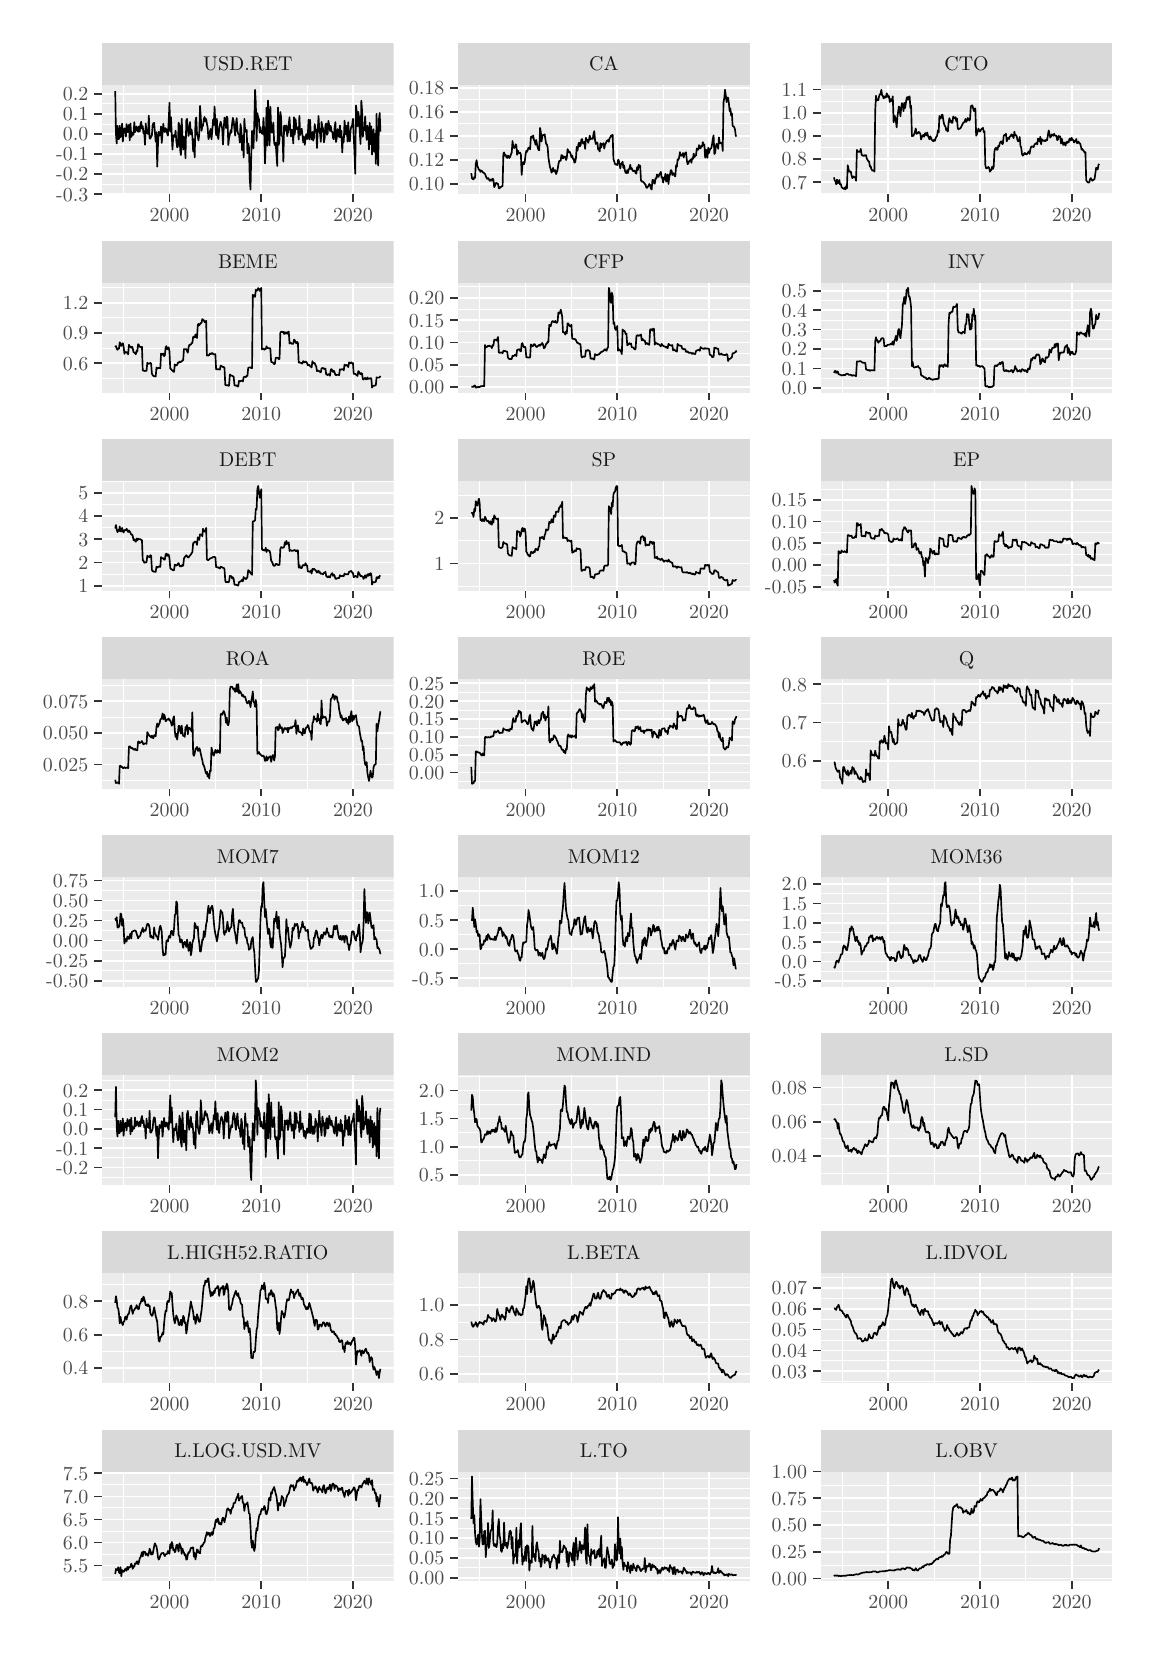
\begin{tikzpicture}[x=1pt,y=1pt]
\definecolor{fillColor}{RGB}{255,255,255}
\path[use as bounding box,fill=fillColor,fill opacity=0.00] (0,0) rectangle (397.48,578.16);
\begin{scope}
\path[clip] (  0.00,  0.00) rectangle (397.48,578.16);
\definecolor{drawColor}{RGB}{255,255,255}
\definecolor{fillColor}{RGB}{255,255,255}

\path[draw=drawColor,line width= 0.6pt,line join=round,line cap=round,fill=fillColor] (  0.00, -0.00) rectangle (397.48,578.16);
\end{scope}
\begin{scope}
\path[clip] ( 26.85,517.89) rectangle (132.26,557.50);
\definecolor{fillColor}{gray}{0.92}

\path[fill=fillColor] ( 26.85,517.89) rectangle (132.26,557.50);
\definecolor{drawColor}{RGB}{255,255,255}

\path[draw=drawColor,line width= 0.3pt,line join=round] ( 26.85,521.62) --
	(132.26,521.62);

\path[draw=drawColor,line width= 0.3pt,line join=round] ( 26.85,528.87) --
	(132.26,528.87);

\path[draw=drawColor,line width= 0.3pt,line join=round] ( 26.85,536.12) --
	(132.26,536.12);

\path[draw=drawColor,line width= 0.3pt,line join=round] ( 26.85,543.36) --
	(132.26,543.36);

\path[draw=drawColor,line width= 0.3pt,line join=round] ( 26.85,550.61) --
	(132.26,550.61);

\path[draw=drawColor,line width= 0.3pt,line join=round] ( 34.67,517.89) --
	( 34.67,557.50);

\path[draw=drawColor,line width= 0.3pt,line join=round] ( 67.82,517.89) --
	( 67.82,557.50);

\path[draw=drawColor,line width= 0.3pt,line join=round] (100.97,517.89) --
	(100.97,557.50);

\path[draw=drawColor,line width= 0.6pt,line join=round] ( 26.85,517.99) --
	(132.26,517.99);

\path[draw=drawColor,line width= 0.6pt,line join=round] ( 26.85,525.24) --
	(132.26,525.24);

\path[draw=drawColor,line width= 0.6pt,line join=round] ( 26.85,532.49) --
	(132.26,532.49);

\path[draw=drawColor,line width= 0.6pt,line join=round] ( 26.85,539.74) --
	(132.26,539.74);

\path[draw=drawColor,line width= 0.6pt,line join=round] ( 26.85,546.99) --
	(132.26,546.99);

\path[draw=drawColor,line width= 0.6pt,line join=round] ( 26.85,554.24) --
	(132.26,554.24);

\path[draw=drawColor,line width= 0.6pt,line join=round] ( 51.25,517.89) --
	( 51.25,557.50);

\path[draw=drawColor,line width= 0.6pt,line join=round] ( 84.40,517.89) --
	( 84.40,557.50);

\path[draw=drawColor,line width= 0.6pt,line join=round] (117.54,517.89) --
	(117.54,557.50);
\definecolor{drawColor}{RGB}{0,0,0}

\path[draw=drawColor,line width= 0.6pt,line join=round] ( 31.64,555.24) --
	( 31.89,539.94) --
	( 32.17,536.29) --
	( 32.44,542.69) --
	( 32.73,537.85) --
	( 33.00,537.97) --
	( 33.26,542.74) --
	( 33.56,538.58) --
	( 33.83,539.55) --
	( 34.12,543.49) --
	( 34.39,536.99) --
	( 34.66,540.93) --
	( 34.95,541.79) --
	( 35.20,541.64) --
	( 35.49,538.82) --
	( 35.74,543.30) --
	( 36.04,540.40) --
	( 36.31,541.42) --
	( 36.59,543.04) --
	( 36.87,537.42) --
	( 37.14,543.53) --
	( 37.43,538.67) --
	( 37.70,539.28) --
	( 37.96,540.23) --
	( 38.26,539.46) --
	( 38.53,544.03) --
	( 38.79,540.39) --
	( 39.08,541.44) --
	( 39.36,542.45) --
	( 39.61,541.06) --
	( 39.91,540.53) --
	( 40.19,542.45) --
	( 40.47,540.64) --
	( 40.75,543.10) --
	( 41.01,544.14) --
	( 41.30,541.67) --
	( 41.58,542.57) --
	( 41.84,539.92) --
	( 42.12,540.71) --
	( 42.39,535.85) --
	( 42.66,543.57) --
	( 42.95,539.97) --
	( 43.23,541.18) --
	( 43.49,539.73) --
	( 43.78,546.37) --
	( 44.06,538.18) --
	( 44.32,538.06) --
	( 44.61,538.79) --
	( 44.89,539.27) --
	( 45.14,542.90) --
	( 45.43,543.65) --
	( 45.70,543.73) --
	( 45.97,540.36) --
	( 46.26,536.97) --
	( 46.54,540.37) --
	( 46.82,527.93) --
	( 47.09,536.03) --
	( 47.36,540.55) --
	( 47.65,539.33) --
	( 47.93,539.26) --
	( 48.19,542.45) --
	( 48.44,536.51) --
	( 48.74,540.35) --
	( 49.02,543.42) --
	( 49.30,540.67) --
	( 49.57,540.44) --
	( 49.84,541.84) --
	( 50.13,541.21) --
	( 50.40,539.93) --
	( 50.67,539.14) --
	( 50.96,544.46) --
	( 51.24,551.06) --
	( 51.52,540.64) --
	( 51.78,545.79) --
	( 52.07,539.43) --
	( 52.32,534.12) --
	( 52.62,539.13) --
	( 52.89,539.36) --
	( 53.17,538.69) --
	( 53.45,540.95) --
	( 53.72,537.07) --
	( 54.01,534.90) --
	( 54.28,535.23) --
	( 54.54,543.83) --
	( 54.84,542.77) --
	( 55.10,534.04) --
	( 55.37,532.14) --
	( 55.65,545.23) --
	( 55.93,538.84) --
	( 56.19,534.08) --
	( 56.48,538.72) --
	( 56.77,536.59) --
	( 57.02,530.93) --
	( 57.32,544.60) --
	( 57.59,545.21) --
	( 57.87,541.35) --
	( 58.15,539.03) --
	( 58.41,541.72) --
	( 58.67,544.04) --
	( 58.96,539.65) --
	( 59.24,541.30) --
	( 59.50,538.96) --
	( 59.80,533.43) --
	( 60.07,537.83) --
	( 60.35,531.27) --
	( 60.63,544.27) --
	( 60.90,545.73) --
	( 61.19,539.81) --
	( 61.47,538.81) --
	( 61.72,537.37) --
	( 62.00,539.65) --
	( 62.27,549.90) --
	( 62.55,545.97) --
	( 62.83,540.90) --
	( 63.11,542.64) --
	( 63.37,542.67) --
	( 63.66,545.22) --
	( 63.94,545.93) --
	( 64.20,544.28) --
	( 64.50,545.16) --
	( 64.77,543.45) --
	( 65.02,542.25) --
	( 65.32,537.89) --
	( 65.60,538.64) --
	( 65.88,540.67) --
	( 66.15,541.56) --
	( 66.42,537.82) --
	( 66.71,541.01) --
	( 66.98,544.88) --
	( 67.25,542.96) --
	( 67.54,549.67) --
	( 67.82,543.18) --
	( 68.10,539.34) --
	( 68.36,545.20) --
	( 68.64,539.04) --
	( 68.90,537.92) --
	( 69.19,541.29) --
	( 69.46,543.13) --
	( 69.73,544.20) --
	( 70.02,543.08) --
	( 70.30,541.60) --
	( 70.58,535.95) --
	( 70.85,541.74) --
	( 71.12,545.64) --
	( 71.41,544.83) --
	( 71.67,541.86) --
	( 71.95,546.03) --
	( 72.20,545.41) --
	( 72.50,535.75) --
	( 72.77,538.34) --
	( 73.06,539.46) --
	( 73.34,541.09) --
	( 73.60,540.18) --
	( 73.89,543.61) --
	( 74.16,545.55) --
	( 74.43,544.43) --
	( 74.73,541.33) --
	( 74.98,539.12) --
	( 75.25,543.32) --
	( 75.53,545.45) --
	( 75.81,540.88) --
	( 76.08,539.74) --
	( 76.37,539.65) --
	( 76.65,536.63) --
	( 76.90,543.32) --
	( 77.20,541.25) --
	( 77.48,533.85) --
	( 77.76,539.11) --
	( 78.04,531.23) --
	( 78.30,545.18) --
	( 78.58,541.02) --
	( 78.85,540.46) --
	( 79.13,541.25) --
	( 79.41,532.72) --
	( 79.69,536.34) --
	( 79.95,535.07) --
	( 80.24,523.65) --
	( 80.52,519.69) --
	( 80.78,531.70) --
	( 81.08,540.88) --
	( 81.35,537.38) --
	( 81.60,534.60) --
	( 81.89,543.95) --
	( 82.17,555.70) --
	( 82.43,551.11) --
	( 82.72,537.22) --
	( 83.00,547.24) --
	( 83.28,545.78) --
	( 83.56,545.09) --
	( 83.83,540.18) --
	( 84.11,542.18) --
	( 84.39,540.43) --
	( 84.65,539.96) --
	( 84.91,539.74) --
	( 85.21,545.56) --
	( 85.48,540.39) --
	( 85.76,529.09) --
	( 86.03,537.22) --
	( 86.31,549.24) --
	( 86.60,535.48) --
	( 86.87,551.86) --
	( 87.13,542.66) --
	( 87.42,535.58) --
	( 87.70,549.58) --
	( 87.98,541.84) --
	( 88.24,540.19) --
	( 88.52,541.86) --
	( 88.78,543.86) --
	( 89.07,536.44) --
	( 89.35,535.64) --
	( 89.61,536.59) --
	( 89.91,532.07) --
	( 90.18,528.15) --
	( 90.46,549.35) --
	( 90.73,535.79) --
	( 91.01,537.61) --
	( 91.30,547.68) --
	( 91.56,545.95) --
	( 91.83,539.03) --
	( 92.11,538.83) --
	( 92.39,529.74) --
	( 92.66,542.87) --
	( 92.95,540.86) --
	( 93.23,542.55) --
	( 93.48,542.87) --
	( 93.78,538.95) --
	( 94.06,540.34) --
	( 94.34,543.36) --
	( 94.62,545.82) --
	( 94.87,541.35) --
	( 95.14,538.82) --
	( 95.43,541.27) --
	( 95.71,540.93) --
	( 95.96,536.26) --
	( 96.26,545.78) --
	( 96.53,539.54) --
	( 96.81,545.11) --
	( 97.10,541.73) --
	( 97.36,541.43) --
	( 97.65,542.10) --
	( 97.93,537.71) --
	( 98.18,546.29) --
	( 98.47,539.37) --
	( 98.74,541.37) --
	( 99.01,541.60) --
	( 99.29,539.46) --
	( 99.57,536.70) --
	( 99.84,538.77) --
	(100.13,535.81) --
	(100.41,538.10) --
	(100.66,539.75) --
	(100.96,537.88) --
	(101.23,539.25) --
	(101.49,544.94) --
	(101.78,537.72) --
	(102.05,544.87) --
	(102.31,539.42) --
	(102.60,537.76) --
	(102.89,540.47) --
	(103.17,537.34) --
	(103.44,538.22) --
	(103.71,543.28) --
	(103.99,541.62) --
	(104.27,541.27) --
	(104.54,534.67) --
	(104.82,540.99) --
	(105.10,546.23) --
	(105.36,541.47) --
	(105.65,539.87) --
	(105.93,536.88) --
	(106.19,544.08) --
	(106.49,542.25) --
	(106.76,541.68) --
	(107.04,536.70) --
	(107.31,538.11) --
	(107.59,542.97) --
	(107.88,543.52) --
	(108.13,539.45) --
	(108.41,539.89) --
	(108.67,544.46) --
	(108.97,542.76) --
	(109.24,540.86) --
	(109.52,542.63) --
	(109.80,540.58) --
	(110.06,540.55) --
	(110.35,538.33) --
	(110.63,537.77) --
	(110.89,541.75) --
	(111.19,544.06) --
	(111.44,536.85) --
	(111.72,538.54) --
	(112.00,541.51) --
	(112.28,540.02) --
	(112.54,538.60) --
	(112.83,542.83) --
	(113.11,538.47) --
	(113.37,540.85) --
	(113.67,533.08) --
	(113.94,538.58) --
	(114.22,536.82) --
	(114.50,544.54) --
	(114.76,541.56) --
	(115.02,539.52) --
	(115.31,542.76) --
	(115.59,536.99) --
	(115.84,544.02) --
	(116.14,537.37) --
	(116.42,537.09) --
	(116.70,541.34) --
	(116.98,542.49) --
	(117.24,542.84) --
	(117.53,545.23) --
	(117.81,538.74) --
	(118.07,533.74) --
	(118.36,525.37) --
	(118.63,550.03) --
	(118.89,548.03) --
	(119.18,542.48) --
	(119.47,547.71) --
	(119.75,545.62) --
	(120.02,539.88) --
	(120.29,536.12) --
	(120.57,551.78) --
	(120.85,547.90) --
	(121.12,538.73) --
	(121.37,541.38) --
	(121.67,541.15) --
	(121.94,546.08) --
	(122.22,541.38) --
	(122.50,537.61) --
	(122.77,542.73) --
	(123.06,541.27) --
	(123.33,534.09) --
	(123.59,543.75) --
	(123.89,536.13) --
	(124.17,542.48) --
	(124.45,532.30) --
	(124.70,535.12) --
	(124.98,541.45) --
	(125.25,533.38) --
	(125.54,539.71) --
	(125.81,528.93) --
	(126.07,547.01) --
	(126.37,533.67) --
	(126.64,528.34) --
	(126.93,544.89) --
	(127.20,547.32) --
	(127.47,540.63);
\end{scope}
\begin{scope}
\path[clip] ( 26.85,446.30) rectangle (132.26,485.92);
\definecolor{fillColor}{gray}{0.92}

\path[fill=fillColor] ( 26.85,446.30) rectangle (132.26,485.92);
\definecolor{drawColor}{RGB}{255,255,255}

\path[draw=drawColor,line width= 0.3pt,line join=round] ( 26.85,451.47) --
	(132.26,451.47);

\path[draw=drawColor,line width= 0.3pt,line join=round] ( 26.85,462.38) --
	(132.26,462.38);

\path[draw=drawColor,line width= 0.3pt,line join=round] ( 26.85,473.29) --
	(132.26,473.29);

\path[draw=drawColor,line width= 0.3pt,line join=round] ( 26.85,484.20) --
	(132.26,484.20);

\path[draw=drawColor,line width= 0.3pt,line join=round] ( 34.67,446.30) --
	( 34.67,485.92);

\path[draw=drawColor,line width= 0.3pt,line join=round] ( 67.82,446.30) --
	( 67.82,485.92);

\path[draw=drawColor,line width= 0.3pt,line join=round] (100.97,446.30) --
	(100.97,485.92);

\path[draw=drawColor,line width= 0.6pt,line join=round] ( 26.85,456.93) --
	(132.26,456.93);

\path[draw=drawColor,line width= 0.6pt,line join=round] ( 26.85,467.83) --
	(132.26,467.83);

\path[draw=drawColor,line width= 0.6pt,line join=round] ( 26.85,478.74) --
	(132.26,478.74);

\path[draw=drawColor,line width= 0.6pt,line join=round] ( 51.25,446.30) --
	( 51.25,485.92);

\path[draw=drawColor,line width= 0.6pt,line join=round] ( 84.40,446.30) --
	( 84.40,485.92);

\path[draw=drawColor,line width= 0.6pt,line join=round] (117.54,446.30) --
	(117.54,485.92);
\definecolor{drawColor}{RGB}{0,0,0}

\path[draw=drawColor,line width= 0.6pt,line join=round] ( 31.64,462.71) --
	( 31.89,463.10) --
	( 32.17,462.29) --
	( 32.44,461.75) --
	( 32.73,462.25) --
	( 33.00,462.21) --
	( 33.26,464.46) --
	( 33.56,463.98) --
	( 33.83,463.15) --
	( 34.12,463.55) --
	( 34.39,464.13) --
	( 34.66,462.99) --
	( 34.95,460.30) --
	( 35.20,460.98) --
	( 35.49,460.82) --
	( 35.74,460.97) --
	( 36.04,460.51) --
	( 36.31,460.14) --
	( 36.59,463.58) --
	( 36.87,463.03) --
	( 37.14,462.81) --
	( 37.43,462.51) --
	( 37.70,462.87) --
	( 37.96,462.29) --
	( 38.26,460.84) --
	( 38.53,460.82) --
	( 38.79,460.56) --
	( 39.08,460.13) --
	( 39.36,461.39) --
	( 39.61,461.10) --
	( 39.91,463.79) --
	( 40.19,463.46) --
	( 40.47,462.83) --
	( 40.75,462.79) --
	( 41.01,462.58) --
	( 41.30,462.82) --
	( 41.58,454.32) --
	( 41.84,454.21) --
	( 42.12,454.13) --
	( 42.39,454.10) --
	( 42.66,454.26) --
	( 42.95,454.10) --
	( 43.23,457.06) --
	( 43.49,456.62) --
	( 43.78,456.88) --
	( 44.06,456.76) --
	( 44.32,457.04) --
	( 44.61,456.73) --
	( 44.89,453.13) --
	( 45.14,452.67) --
	( 45.43,452.30) --
	( 45.70,452.14) --
	( 45.97,452.21) --
	( 46.26,452.10) --
	( 46.54,455.34) --
	( 46.82,454.93) --
	( 47.09,455.19) --
	( 47.36,455.12) --
	( 47.65,455.35) --
	( 47.93,455.06) --
	( 48.19,460.39) --
	( 48.44,459.84) --
	( 48.74,460.32) --
	( 49.02,460.38) --
	( 49.30,459.43) --
	( 49.57,459.78) --
	( 49.84,462.56) --
	( 50.13,463.10) --
	( 50.40,461.89) --
	( 50.67,462.45) --
	( 50.96,462.59) --
	( 51.24,461.10) --
	( 51.52,454.95) --
	( 51.78,454.79) --
	( 52.07,454.38) --
	( 52.32,454.30) --
	( 52.62,453.89) --
	( 52.89,453.76) --
	( 53.17,456.50) --
	( 53.45,456.10) --
	( 53.72,456.12) --
	( 54.01,456.32) --
	( 54.28,457.11) --
	( 54.54,457.02) --
	( 54.84,457.50) --
	( 55.10,457.21) --
	( 55.37,457.45) --
	( 55.65,457.51) --
	( 55.93,457.91) --
	( 56.19,457.98) --
	( 56.48,462.00) --
	( 56.77,461.93) --
	( 57.02,461.99) --
	( 57.32,462.00) --
	( 57.59,461.34) --
	( 57.87,460.70) --
	( 58.15,462.65) --
	( 58.41,463.50) --
	( 58.67,463.61) --
	( 58.96,463.59) --
	( 59.24,464.19) --
	( 59.50,464.19) --
	( 59.80,466.44) --
	( 60.07,466.44) --
	( 60.35,466.20) --
	( 60.63,467.31) --
	( 60.90,466.28) --
	( 61.19,466.02) --
	( 61.47,470.68) --
	( 61.72,471.12) --
	( 62.00,470.57) --
	( 62.27,471.10) --
	( 62.55,471.41) --
	( 62.83,471.47) --
	( 63.11,472.86) --
	( 63.37,472.59) --
	( 63.66,472.41) --
	( 63.94,471.76) --
	( 64.20,471.97) --
	( 64.50,472.22) --
	( 64.77,459.67) --
	( 65.02,459.81) --
	( 65.32,459.64) --
	( 65.60,459.92) --
	( 65.88,460.42) --
	( 66.15,460.17) --
	( 66.42,460.44) --
	( 66.71,460.62) --
	( 66.98,460.26) --
	( 67.25,460.06) --
	( 67.54,460.13) --
	( 67.82,460.21) --
	( 68.10,454.66) --
	( 68.36,454.74) --
	( 68.64,454.77) --
	( 68.90,454.71) --
	( 69.19,454.68) --
	( 69.46,454.57) --
	( 69.73,456.06) --
	( 70.02,455.84) --
	( 70.30,455.73) --
	( 70.58,455.51) --
	( 70.85,455.53) --
	( 71.12,455.20) --
	( 71.41,449.03) --
	( 71.67,448.96) --
	( 71.95,448.91) --
	( 72.20,449.02) --
	( 72.50,448.73) --
	( 72.77,448.78) --
	( 73.06,452.86) --
	( 73.34,452.47) --
	( 73.60,452.49) --
	( 73.89,452.32) --
	( 74.16,452.22) --
	( 74.43,452.02) --
	( 74.73,448.92) --
	( 74.98,448.85) --
	( 75.25,448.89) --
	( 75.53,448.83) --
	( 75.81,448.50) --
	( 76.08,448.53) --
	( 76.37,450.53) --
	( 76.65,450.42) --
	( 76.90,450.39) --
	( 77.20,450.60) --
	( 77.48,450.55) --
	( 77.76,450.32) --
	( 78.04,451.82) --
	( 78.30,452.00) --
	( 78.58,451.99) --
	( 78.85,451.85) --
	( 79.13,452.39) --
	( 79.41,452.30) --
	( 79.69,455.24) --
	( 79.95,455.33) --
	( 80.24,455.42) --
	( 80.52,455.35) --
	( 80.78,455.18) --
	( 81.08,455.14) --
	( 81.35,481.63) --
	( 81.60,480.83) --
	( 81.89,481.53) --
	( 82.17,480.87) --
	( 82.43,483.47) --
	( 82.72,483.03) --
	( 83.00,483.29) --
	( 83.28,484.03) --
	( 83.56,483.84) --
	( 83.83,483.08) --
	( 84.11,483.53) --
	( 84.39,484.12) --
	( 84.65,461.87) --
	( 84.91,462.14) --
	( 85.21,462.13) --
	( 85.48,461.78) --
	( 85.76,462.06) --
	( 86.03,462.05) --
	( 86.31,463.01) --
	( 86.60,462.34) --
	( 86.87,462.41) --
	( 87.13,462.21) --
	( 87.42,462.43) --
	( 87.70,462.08) --
	( 87.98,457.37) --
	( 88.24,457.34) --
	( 88.52,457.21) --
	( 88.78,456.94) --
	( 89.07,456.55) --
	( 89.35,456.78) --
	( 89.61,458.80) --
	( 89.91,458.88) --
	( 90.18,458.88) --
	( 90.46,458.87) --
	( 90.73,458.36) --
	( 91.01,458.46) --
	( 91.30,467.89) --
	( 91.56,468.26) --
	( 91.83,468.28) --
	( 92.11,468.07) --
	( 92.39,468.25) --
	( 92.66,467.45) --
	( 92.95,468.12) --
	( 93.23,467.62) --
	( 93.48,468.03) --
	( 93.78,467.53) --
	( 94.06,468.21) --
	( 94.34,468.32) --
	( 94.62,463.99) --
	( 94.87,464.45) --
	( 95.14,464.19) --
	( 95.43,463.94) --
	( 95.71,463.87) --
	( 95.96,463.95) --
	( 96.26,465.41) --
	( 96.53,465.20) --
	( 96.81,464.45) --
	( 97.10,464.08) --
	( 97.36,464.61) --
	( 97.65,464.18) --
	( 97.93,457.15) --
	( 98.18,457.32) --
	( 98.47,457.02) --
	( 98.74,457.10) --
	( 99.01,456.79) --
	( 99.29,456.83) --
	( 99.57,457.67) --
	( 99.84,457.38) --
	(100.13,457.21) --
	(100.41,457.52) --
	(100.66,457.35) --
	(100.96,456.94) --
	(101.23,456.14) --
	(101.49,456.35) --
	(101.78,456.28) --
	(102.05,455.82) --
	(102.31,455.72) --
	(102.60,455.35) --
	(102.89,457.64) --
	(103.17,456.99) --
	(103.44,456.91) --
	(103.71,456.98) --
	(103.99,456.19) --
	(104.27,455.73) --
	(104.54,454.03) --
	(104.82,454.16) --
	(105.10,454.21) --
	(105.36,454.03) --
	(105.65,453.75) --
	(105.93,453.61) --
	(106.19,455.04) --
	(106.49,455.15) --
	(106.76,455.17) --
	(107.04,454.91) --
	(107.31,454.76) --
	(107.59,454.99) --
	(107.88,452.81) --
	(108.13,452.95) --
	(108.41,452.62) --
	(108.67,453.00) --
	(108.97,452.88) --
	(109.24,452.37) --
	(109.52,454.58) --
	(109.80,454.77) --
	(110.06,454.25) --
	(110.35,453.75) --
	(110.63,454.18) --
	(110.89,453.63) --
	(111.19,452.72) --
	(111.44,452.58) --
	(111.72,452.72) --
	(112.00,452.75) --
	(112.28,452.71) --
	(112.54,452.55) --
	(112.83,454.72) --
	(113.11,454.55) --
	(113.37,454.68) --
	(113.67,454.81) --
	(113.94,454.63) --
	(114.22,454.35) --
	(114.50,456.40) --
	(114.76,456.21) --
	(115.02,455.98) --
	(115.31,456.27) --
	(115.59,455.91) --
	(115.84,455.50) --
	(116.14,457.19) --
	(116.42,456.99) --
	(116.70,456.97) --
	(116.98,457.23) --
	(117.24,456.81) --
	(117.53,456.97) --
	(117.81,453.08) --
	(118.07,453.13) --
	(118.36,453.10) --
	(118.63,452.74) --
	(118.89,452.71) --
	(119.18,452.30) --
	(119.47,454.06) --
	(119.75,453.75) --
	(120.02,453.20) --
	(120.29,452.96) --
	(120.57,453.35) --
	(120.85,453.02) --
	(121.12,451.11) --
	(121.37,451.00) --
	(121.67,451.36) --
	(121.94,451.61) --
	(122.22,451.13) --
	(122.50,451.08) --
	(122.77,451.75) --
	(123.06,451.24) --
	(123.33,451.31) --
	(123.59,451.33) --
	(123.89,451.57) --
	(124.17,451.39) --
	(124.45,448.10) --
	(124.70,448.70) --
	(124.98,448.74) --
	(125.25,448.79) --
	(125.54,448.85) --
	(125.81,449.01) --
	(126.07,451.78) --
	(126.37,451.73) --
	(126.64,451.69) --
	(126.93,451.69) --
	(127.20,451.86) --
	(127.47,452.29);
\end{scope}
\begin{scope}
\path[clip] ( 26.85,374.72) rectangle (132.26,414.34);
\definecolor{fillColor}{gray}{0.92}

\path[fill=fillColor] ( 26.85,374.72) rectangle (132.26,414.34);
\definecolor{drawColor}{RGB}{255,255,255}

\path[draw=drawColor,line width= 0.3pt,line join=round] ( 26.85,380.69) --
	(132.26,380.69);

\path[draw=drawColor,line width= 0.3pt,line join=round] ( 26.85,389.08) --
	(132.26,389.08);

\path[draw=drawColor,line width= 0.3pt,line join=round] ( 26.85,397.48) --
	(132.26,397.48);

\path[draw=drawColor,line width= 0.3pt,line join=round] ( 26.85,405.88) --
	(132.26,405.88);

\path[draw=drawColor,line width= 0.3pt,line join=round] ( 26.85,414.27) --
	(132.26,414.27);

\path[draw=drawColor,line width= 0.3pt,line join=round] ( 34.67,374.72) --
	( 34.67,414.34);

\path[draw=drawColor,line width= 0.3pt,line join=round] ( 67.82,374.72) --
	( 67.82,414.34);

\path[draw=drawColor,line width= 0.3pt,line join=round] (100.97,374.72) --
	(100.97,414.34);

\path[draw=drawColor,line width= 0.6pt,line join=round] ( 26.85,376.49) --
	(132.26,376.49);

\path[draw=drawColor,line width= 0.6pt,line join=round] ( 26.85,384.89) --
	(132.26,384.89);

\path[draw=drawColor,line width= 0.6pt,line join=round] ( 26.85,393.28) --
	(132.26,393.28);

\path[draw=drawColor,line width= 0.6pt,line join=round] ( 26.85,401.68) --
	(132.26,401.68);

\path[draw=drawColor,line width= 0.6pt,line join=round] ( 26.85,410.07) --
	(132.26,410.07);

\path[draw=drawColor,line width= 0.6pt,line join=round] ( 51.25,374.72) --
	( 51.25,414.34);

\path[draw=drawColor,line width= 0.6pt,line join=round] ( 84.40,374.72) --
	( 84.40,414.34);

\path[draw=drawColor,line width= 0.6pt,line join=round] (117.54,374.72) --
	(117.54,414.34);
\definecolor{drawColor}{RGB}{0,0,0}

\path[draw=drawColor,line width= 0.6pt,line join=round] ( 31.64,397.19) --
	( 31.89,398.43) --
	( 32.17,396.86) --
	( 32.44,395.86) --
	( 32.73,396.63) --
	( 33.00,396.24) --
	( 33.26,397.89) --
	( 33.56,396.17) --
	( 33.83,396.11) --
	( 34.12,397.40) --
	( 34.39,396.23) --
	( 34.66,395.73) --
	( 34.95,396.63) --
	( 35.20,396.57) --
	( 35.49,396.48) --
	( 35.74,397.11) --
	( 36.04,396.44) --
	( 36.31,395.91) --
	( 36.59,396.46) --
	( 36.87,396.09) --
	( 37.14,395.56) --
	( 37.43,394.99) --
	( 37.70,395.05) --
	( 37.96,394.49) --
	( 38.26,392.99) --
	( 38.53,393.29) --
	( 38.79,392.73) --
	( 39.08,392.40) --
	( 39.36,393.54) --
	( 39.61,392.88) --
	( 39.91,393.55) --
	( 40.19,393.32) --
	( 40.47,393.35) --
	( 40.75,393.30) --
	( 41.01,393.08) --
	( 41.30,392.97) --
	( 41.58,385.65) --
	( 41.84,385.53) --
	( 42.12,384.89) --
	( 42.39,384.82) --
	( 42.66,384.98) --
	( 42.95,384.98) --
	( 43.23,387.34) --
	( 43.49,386.88) --
	( 43.78,387.14) --
	( 44.06,386.85) --
	( 44.32,387.52) --
	( 44.61,387.34) --
	( 44.89,382.26) --
	( 45.14,381.77) --
	( 45.43,381.71) --
	( 45.70,381.50) --
	( 45.97,381.58) --
	( 46.26,381.48) --
	( 46.54,383.39) --
	( 46.82,383.05) --
	( 47.09,383.30) --
	( 47.36,383.34) --
	( 47.65,383.58) --
	( 47.93,383.29) --
	( 48.19,386.87) --
	( 48.44,386.41) --
	( 48.74,386.50) --
	( 49.02,386.39) --
	( 49.30,385.87) --
	( 49.57,386.01) --
	( 49.84,387.73) --
	( 50.13,388.08) --
	( 50.40,387.27) --
	( 50.67,387.87) --
	( 50.96,387.63) --
	( 51.24,386.46) --
	( 51.52,382.86) --
	( 51.78,382.54) --
	( 52.07,382.39) --
	( 52.32,382.24) --
	( 52.62,382.05) --
	( 52.89,382.16) --
	( 53.17,384.14) --
	( 53.45,383.99) --
	( 53.72,383.77) --
	( 54.01,383.97) --
	( 54.28,384.48) --
	( 54.54,384.68) --
	( 54.84,383.78) --
	( 55.10,383.46) --
	( 55.37,383.69) --
	( 55.65,383.52) --
	( 55.93,384.05) --
	( 56.19,383.72) --
	( 56.48,386.32) --
	( 56.77,386.88) --
	( 57.02,387.10) --
	( 57.32,387.53) --
	( 57.59,387.19) --
	( 57.87,386.78) --
	( 58.15,386.68) --
	( 58.41,387.14) --
	( 58.67,387.44) --
	( 58.96,387.81) --
	( 59.24,388.28) --
	( 59.50,388.60) --
	( 59.80,391.92) --
	( 60.07,392.01) --
	( 60.35,392.41) --
	( 60.63,392.42) --
	( 60.90,392.22) --
	( 61.19,391.27) --
	( 61.47,394.01) --
	( 61.72,393.80) --
	( 62.00,393.09) --
	( 62.27,395.09) --
	( 62.55,394.93) --
	( 62.83,395.06) --
	( 63.11,394.38) --
	( 63.37,397.08) --
	( 63.66,396.14) --
	( 63.94,396.10) --
	( 64.20,396.24) --
	( 64.50,397.39) --
	( 64.77,386.04) --
	( 65.02,385.82) --
	( 65.32,385.76) --
	( 65.60,386.08) --
	( 65.88,386.28) --
	( 66.15,386.44) --
	( 66.42,386.56) --
	( 66.71,386.63) --
	( 66.98,386.92) --
	( 67.25,386.92) --
	( 67.54,386.88) --
	( 67.82,386.81) --
	( 68.10,383.20) --
	( 68.36,383.27) --
	( 68.64,383.07) --
	( 68.90,383.17) --
	( 69.19,382.87) --
	( 69.46,382.73) --
	( 69.73,383.40) --
	( 70.02,383.32) --
	( 70.30,383.07) --
	( 70.58,382.94) --
	( 70.85,382.96) --
	( 71.12,382.43) --
	( 71.41,378.27) --
	( 71.67,377.74) --
	( 71.95,377.86) --
	( 72.20,377.87) --
	( 72.50,377.72) --
	( 72.77,378.02) --
	( 73.06,380.11) --
	( 73.34,379.94) --
	( 73.60,379.99) --
	( 73.89,379.08) --
	( 74.16,379.54) --
	( 74.43,379.03) --
	( 74.73,376.87) --
	( 74.98,376.82) --
	( 75.25,376.84) --
	( 75.53,376.79) --
	( 75.81,376.63) --
	( 76.08,376.52) --
	( 76.37,377.88) --
	( 76.65,377.87) --
	( 76.90,378.15) --
	( 77.20,378.21) --
	( 77.48,378.67) --
	( 77.76,378.09) --
	( 78.04,379.64) --
	( 78.30,379.13) --
	( 78.58,379.28) --
	( 78.85,378.87) --
	( 79.13,379.16) --
	( 79.41,379.66) --
	( 79.69,382.13) --
	( 79.95,381.91) --
	( 80.24,381.66) --
	( 80.52,381.05) --
	( 80.78,380.73) --
	( 81.08,380.45) --
	( 81.35,399.77) --
	( 81.60,399.79) --
	( 81.89,399.86) --
	( 82.17,400.20) --
	( 82.43,404.26) --
	( 82.72,404.06) --
	( 83.00,411.40) --
	( 83.28,412.54) --
	( 83.56,410.69) --
	( 83.83,408.26) --
	( 84.11,408.97) --
	( 84.39,411.40) --
	( 84.65,389.76) --
	( 84.91,389.39) --
	( 85.21,389.42) --
	( 85.48,389.22) --
	( 85.76,389.25) --
	( 86.03,390.21) --
	( 86.31,388.70) --
	( 86.60,389.49) --
	( 86.87,389.33) --
	( 87.13,389.15) --
	( 87.42,389.06) --
	( 87.70,388.08) --
	( 87.98,385.56) --
	( 88.24,385.21) --
	( 88.52,384.62) --
	( 88.78,383.81) --
	( 89.07,383.67) --
	( 89.35,383.72) --
	( 89.61,384.33) --
	( 89.91,384.40) --
	( 90.18,384.21) --
	( 90.46,383.96) --
	( 90.73,384.09) --
	( 91.01,384.07) --
	( 91.30,389.81) --
	( 91.56,390.44) --
	( 91.83,390.38) --
	( 92.11,390.20) --
	( 92.39,390.29) --
	( 92.66,390.53) --
	( 92.95,392.21) --
	( 93.23,391.35) --
	( 93.48,392.70) --
	( 93.78,391.60) --
	( 94.06,391.73) --
	( 94.34,392.14) --
	( 94.62,389.04) --
	( 94.87,389.40) --
	( 95.14,389.31) --
	( 95.43,389.07) --
	( 95.71,389.15) --
	( 95.96,389.18) --
	( 96.26,389.34) --
	( 96.53,389.41) --
	( 96.81,389.07) --
	( 97.10,388.95) --
	( 97.36,389.34) --
	( 97.65,389.24) --
	( 97.93,383.00) --
	( 98.18,383.93) --
	( 98.47,383.07) --
	( 98.74,382.90) --
	( 99.01,382.85) --
	( 99.29,383.68) --
	( 99.57,384.03) --
	( 99.84,383.82) --
	(100.13,383.86) --
	(100.41,384.66) --
	(100.66,383.94) --
	(100.96,383.82) --
	(101.23,381.69) --
	(101.49,381.61) --
	(101.78,381.57) --
	(102.05,381.51) --
	(102.31,382.05) --
	(102.60,380.89) --
	(102.89,382.59) --
	(103.17,382.26) --
	(103.44,382.61) --
	(103.71,382.32) --
	(103.99,382.17) --
	(104.27,381.70) --
	(104.54,381.23) --
	(104.82,381.74) --
	(105.10,381.91) --
	(105.36,381.19) --
	(105.65,381.41) --
	(105.93,380.78) --
	(106.19,380.87) --
	(106.49,380.78) --
	(106.76,380.63) --
	(107.04,381.22) --
	(107.31,381.17) --
	(107.59,381.55) --
	(107.88,380.02) --
	(108.13,379.84) --
	(108.41,379.55) --
	(108.67,379.92) --
	(108.97,379.59) --
	(109.24,379.52) --
	(109.52,380.39) --
	(109.80,380.70) --
	(110.06,381.06) --
	(110.35,380.07) --
	(110.63,380.50) --
	(110.89,380.15) --
	(111.19,379.09) --
	(111.44,378.93) --
	(111.72,379.22) --
	(112.00,379.18) --
	(112.28,379.28) --
	(112.54,379.27) --
	(112.83,380.33) --
	(113.11,379.95) --
	(113.37,379.97) --
	(113.67,380.15) --
	(113.94,379.92) --
	(114.22,379.99) --
	(114.50,380.92) --
	(114.76,380.61) --
	(115.02,380.63) --
	(115.31,380.68) --
	(115.59,380.61) --
	(115.84,380.62) --
	(116.14,381.53) --
	(116.42,381.58) --
	(116.70,381.79) --
	(116.98,381.85) --
	(117.24,381.23) --
	(117.53,381.12) --
	(117.81,379.58) --
	(118.07,379.74) --
	(118.36,380.07) --
	(118.63,379.87) --
	(118.89,379.73) --
	(119.18,379.51) --
	(119.47,381.48) --
	(119.75,381.02) --
	(120.02,380.50) --
	(120.29,379.97) --
	(120.57,380.15) --
	(120.85,379.88) --
	(121.12,379.67) --
	(121.37,378.98) --
	(121.67,379.56) --
	(121.94,380.32) --
	(122.22,379.33) --
	(122.50,379.92) --
	(122.77,380.63) --
	(123.06,380.07) --
	(123.33,380.80) --
	(123.59,380.25) --
	(123.89,381.05) --
	(124.17,380.71) --
	(124.45,376.89) --
	(124.70,377.83) --
	(124.98,377.81) --
	(125.25,377.73) --
	(125.54,377.82) --
	(125.81,377.97) --
	(126.07,379.58) --
	(126.37,379.08) --
	(126.64,379.71) --
	(126.93,379.24) --
	(127.20,380.09) --
	(127.47,380.19);
\end{scope}
\begin{scope}
\path[clip] ( 26.85,303.14) rectangle (132.26,342.75);
\definecolor{fillColor}{gray}{0.92}

\path[fill=fillColor] ( 26.85,303.14) rectangle (132.26,342.75);
\definecolor{drawColor}{RGB}{255,255,255}

\path[draw=drawColor,line width= 0.3pt,line join=round] ( 26.85,306.21) --
	(132.26,306.21);

\path[draw=drawColor,line width= 0.3pt,line join=round] ( 26.85,317.64) --
	(132.26,317.64);

\path[draw=drawColor,line width= 0.3pt,line join=round] ( 26.85,329.06) --
	(132.26,329.06);

\path[draw=drawColor,line width= 0.3pt,line join=round] ( 26.85,340.49) --
	(132.26,340.49);

\path[draw=drawColor,line width= 0.3pt,line join=round] ( 34.67,303.14) --
	( 34.67,342.75);

\path[draw=drawColor,line width= 0.3pt,line join=round] ( 67.82,303.14) --
	( 67.82,342.75);

\path[draw=drawColor,line width= 0.3pt,line join=round] (100.97,303.14) --
	(100.97,342.75);

\path[draw=drawColor,line width= 0.6pt,line join=round] ( 26.85,311.92) --
	(132.26,311.92);

\path[draw=drawColor,line width= 0.6pt,line join=round] ( 26.85,323.35) --
	(132.26,323.35);

\path[draw=drawColor,line width= 0.6pt,line join=round] ( 26.85,334.78) --
	(132.26,334.78);

\path[draw=drawColor,line width= 0.6pt,line join=round] ( 51.25,303.14) --
	( 51.25,342.75);

\path[draw=drawColor,line width= 0.6pt,line join=round] ( 84.40,303.14) --
	( 84.40,342.75);

\path[draw=drawColor,line width= 0.6pt,line join=round] (117.54,303.14) --
	(117.54,342.75);
\definecolor{drawColor}{RGB}{0,0,0}

\path[draw=drawColor,line width= 0.6pt,line join=round] ( 31.64,306.37) --
	( 31.89,305.20) --
	( 32.17,305.31) --
	( 32.44,305.45) --
	( 32.73,305.28) --
	( 33.00,304.94) --
	( 33.26,311.33) --
	( 33.56,311.50) --
	( 33.83,310.97) --
	( 34.12,311.03) --
	( 34.39,310.59) --
	( 34.66,310.62) --
	( 34.95,310.93) --
	( 35.20,310.63) --
	( 35.49,310.74) --
	( 35.74,310.67) --
	( 36.04,310.88) --
	( 36.31,310.57) --
	( 36.59,318.36) --
	( 36.87,318.51) --
	( 37.14,318.20) --
	( 37.43,317.73) --
	( 37.70,317.95) --
	( 37.96,317.63) --
	( 38.26,317.40) --
	( 38.53,317.19) --
	( 38.79,317.57) --
	( 39.08,317.14) --
	( 39.36,317.18) --
	( 39.61,317.00) --
	( 39.91,320.20) --
	( 40.19,320.19) --
	( 40.47,319.63) --
	( 40.75,319.86) --
	( 41.01,319.94) --
	( 41.30,320.38) --
	( 41.58,319.74) --
	( 41.84,319.16) --
	( 42.12,319.44) --
	( 42.39,319.53) --
	( 42.66,319.55) --
	( 42.95,319.35) --
	( 43.23,323.61) --
	( 43.49,323.02) --
	( 43.78,322.61) --
	( 44.06,322.15) --
	( 44.32,322.16) --
	( 44.61,321.64) --
	( 44.89,322.35) --
	( 45.14,321.57) --
	( 45.43,321.47) --
	( 45.70,322.49) --
	( 45.97,322.56) --
	( 46.26,322.10) --
	( 46.54,325.50) --
	( 46.82,326.75) --
	( 47.09,325.50) --
	( 47.36,326.27) --
	( 47.65,326.76) --
	( 47.93,328.09) --
	( 48.19,328.39) --
	( 48.44,328.66) --
	( 48.74,330.33) --
	( 49.02,328.22) --
	( 49.30,329.97) --
	( 49.57,329.27) --
	( 49.84,327.55) --
	( 50.13,327.73) --
	( 50.40,328.21) --
	( 50.67,328.23) --
	( 50.96,328.55) --
	( 51.24,327.77) --
	( 51.52,327.91) --
	( 51.78,327.08) --
	( 52.07,325.96) --
	( 52.32,326.32) --
	( 52.62,328.68) --
	( 52.89,329.31) --
	( 53.17,324.00) --
	( 53.45,321.84) --
	( 53.72,323.02) --
	( 54.01,320.88) --
	( 54.28,322.97) --
	( 54.54,325.89) --
	( 54.84,325.79) --
	( 55.10,323.91) --
	( 55.37,323.11) --
	( 55.65,325.95) --
	( 55.93,323.36) --
	( 56.19,322.27) --
	( 56.48,322.36) --
	( 56.77,321.87) --
	( 57.02,325.40) --
	( 57.32,324.64) --
	( 57.59,326.19) --
	( 57.87,322.78) --
	( 58.15,325.15) --
	( 58.41,325.18) --
	( 58.67,324.69) --
	( 58.96,324.52) --
	( 59.24,323.82) --
	( 59.50,330.75) --
	( 59.80,315.69) --
	( 60.07,315.03) --
	( 60.35,315.87) --
	( 60.63,317.56) --
	( 60.90,317.74) --
	( 61.19,318.27) --
	( 61.47,316.84) --
	( 61.72,316.83) --
	( 62.00,317.78) --
	( 62.27,317.20) --
	( 62.55,315.76) --
	( 62.83,314.54) --
	( 63.11,313.45) --
	( 63.37,311.95) --
	( 63.66,311.55) --
	( 63.94,310.67) --
	( 64.20,309.49) --
	( 64.50,308.59) --
	( 64.77,309.26) --
	( 65.02,307.56) --
	( 65.32,308.40) --
	( 65.60,306.87) --
	( 65.88,309.73) --
	( 66.15,309.47) --
	( 66.42,318.00) --
	( 66.71,316.80) --
	( 66.98,315.68) --
	( 67.25,315.08) --
	( 67.54,316.02) --
	( 67.82,317.16) --
	( 68.10,316.41) --
	( 68.36,316.09) --
	( 68.64,317.14) --
	( 68.90,316.36) --
	( 69.19,316.84) --
	( 69.46,316.01) --
	( 69.73,330.03) --
	( 70.02,330.30) --
	( 70.30,329.87) --
	( 70.58,330.68) --
	( 70.85,331.23) --
	( 71.12,330.57) --
	( 71.41,329.41) --
	( 71.67,327.00) --
	( 71.95,328.83) --
	( 72.20,326.36) --
	( 72.50,326.10) --
	( 72.77,327.49) --
	( 73.06,338.89) --
	( 73.34,340.06) --
	( 73.60,339.93) --
	( 73.89,340.01) --
	( 74.16,339.45) --
	( 74.43,338.86) --
	( 74.73,339.39) --
	( 74.98,338.13) --
	( 75.25,338.55) --
	( 75.53,340.80) --
	( 75.81,338.20) --
	( 76.08,340.95) --
	( 76.37,337.62) --
	( 76.65,338.48) --
	( 76.90,338.07) --
	( 77.20,337.55) --
	( 77.48,336.66) --
	( 77.76,337.07) --
	( 78.04,336.31) --
	( 78.30,336.48) --
	( 78.58,336.42) --
	( 78.85,335.34) --
	( 79.13,334.40) --
	( 79.41,333.97) --
	( 79.69,334.18) --
	( 79.95,334.91) --
	( 80.24,334.34) --
	( 80.52,332.63) --
	( 80.78,334.77) --
	( 81.08,336.38) --
	( 81.35,338.32) --
	( 81.60,334.48) --
	( 81.89,334.33) --
	( 82.17,332.74) --
	( 82.43,335.23) --
	( 82.72,333.21) --
	( 83.00,315.76) --
	( 83.28,315.98) --
	( 83.56,316.42) --
	( 83.83,315.72) --
	( 84.11,315.62) --
	( 84.39,315.23) --
	( 84.65,314.97) --
	( 84.91,314.92) --
	( 85.21,315.07) --
	( 85.48,314.49) --
	( 85.76,313.20) --
	( 86.03,313.24) --
	( 86.31,314.86) --
	( 86.60,313.45) --
	( 86.87,314.00) --
	( 87.13,314.50) --
	( 87.42,314.68) --
	( 87.70,314.89) --
	( 87.98,312.84) --
	( 88.24,314.07) --
	( 88.52,315.32) --
	( 88.78,315.19) --
	( 89.07,313.35) --
	( 89.35,314.92) --
	( 89.61,325.26) --
	( 89.91,325.25) --
	( 90.18,325.49) --
	( 90.46,324.29) --
	( 90.73,324.51) --
	( 91.01,326.49) --
	( 91.30,325.19) --
	( 91.56,325.05) --
	( 91.83,325.39) --
	( 92.11,323.29) --
	( 92.39,323.86) --
	( 92.66,324.81) --
	( 92.95,325.12) --
	( 93.23,324.74) --
	( 93.48,324.53) --
	( 93.78,325.13) --
	( 94.06,323.52) --
	( 94.34,325.10) --
	( 94.62,324.80) --
	( 94.87,325.22) --
	( 95.14,325.42) --
	( 95.43,325.03) --
	( 95.71,325.69) --
	( 95.96,325.66) --
	( 96.26,325.70) --
	( 96.53,326.07) --
	( 96.81,327.92) --
	( 97.10,322.96) --
	( 97.36,325.08) --
	( 97.65,326.06) --
	( 97.93,324.07) --
	( 98.18,323.59) --
	( 98.47,323.65) --
	( 98.74,323.41) --
	( 99.01,323.10) --
	( 99.29,322.47) --
	( 99.57,324.94) --
	( 99.84,323.37) --
	(100.13,323.14) --
	(100.41,324.70) --
	(100.66,325.29) --
	(100.96,325.36) --
	(101.23,326.19) --
	(101.49,325.78) --
	(101.78,324.24) --
	(102.05,323.63) --
	(102.31,323.91) --
	(102.60,320.80) --
	(102.89,326.83) --
	(103.17,327.26) --
	(103.44,329.38) --
	(103.71,328.13) --
	(103.99,328.34) --
	(104.27,328.45) --
	(104.54,327.32) --
	(104.82,330.27) --
	(105.10,327.94) --
	(105.36,328.37) --
	(105.65,326.76) --
	(105.93,326.50) --
	(106.19,335.04) --
	(106.49,328.62) --
	(106.76,329.35) --
	(107.04,328.87) --
	(107.31,329.03) --
	(107.59,329.13) --
	(107.88,328.35) --
	(108.13,325.86) --
	(108.41,327.00) --
	(108.67,327.51) --
	(108.97,327.38) --
	(109.24,329.44) --
	(109.52,335.46) --
	(109.80,335.75) --
	(110.06,336.23) --
	(110.35,337.31) --
	(110.63,336.51) --
	(110.89,335.31) --
	(111.19,336.60) --
	(111.44,336.49) --
	(111.72,336.33) --
	(112.00,334.60) --
	(112.28,334.23) --
	(112.54,331.76) --
	(112.83,330.59) --
	(113.11,328.87) --
	(113.37,329.69) --
	(113.67,328.28) --
	(113.94,327.80) --
	(114.22,328.50) --
	(114.50,328.45) --
	(114.76,327.99) --
	(115.02,328.73) --
	(115.31,327.13) --
	(115.59,328.16) --
	(115.84,326.54) --
	(116.14,329.30) --
	(116.42,327.14) --
	(116.70,329.67) --
	(116.98,331.20) --
	(117.24,327.47) --
	(117.53,329.59) --
	(117.81,328.06) --
	(118.07,329.26) --
	(118.36,329.46) --
	(118.63,329.72) --
	(118.89,327.71) --
	(119.18,326.14) --
	(119.47,325.89) --
	(119.75,325.51) --
	(120.02,323.29) --
	(120.29,321.95) --
	(120.57,320.32) --
	(120.85,320.52) --
	(121.12,316.99) --
	(121.37,318.34) --
	(121.67,313.70) --
	(121.94,312.07) --
	(122.22,311.59) --
	(122.50,312.76) --
	(122.77,308.80) --
	(123.06,307.29) --
	(123.33,305.97) --
	(123.59,307.41) --
	(123.89,309.65) --
	(124.17,307.80) --
	(124.45,307.16) --
	(124.70,307.57) --
	(124.98,310.88) --
	(125.25,311.64) --
	(125.54,311.89) --
	(125.81,312.12) --
	(126.07,326.61) --
	(126.37,323.86) --
	(126.64,326.04) --
	(126.93,327.54) --
	(127.20,329.39) --
	(127.47,331.13);
\end{scope}
\begin{scope}
\path[clip] ( 26.85,231.56) rectangle (132.26,271.17);
\definecolor{fillColor}{gray}{0.92}

\path[fill=fillColor] ( 26.85,231.56) rectangle (132.26,271.17);
\definecolor{drawColor}{RGB}{255,255,255}

\path[draw=drawColor,line width= 0.3pt,line join=round] ( 26.85,237.38) --
	(132.26,237.38);

\path[draw=drawColor,line width= 0.3pt,line join=round] ( 26.85,244.63) --
	(132.26,244.63);

\path[draw=drawColor,line width= 0.3pt,line join=round] ( 26.85,251.89) --
	(132.26,251.89);

\path[draw=drawColor,line width= 0.3pt,line join=round] ( 26.85,259.15) --
	(132.26,259.15);

\path[draw=drawColor,line width= 0.3pt,line join=round] ( 26.85,266.40) --
	(132.26,266.40);

\path[draw=drawColor,line width= 0.3pt,line join=round] ( 34.67,231.56) --
	( 34.67,271.17);

\path[draw=drawColor,line width= 0.3pt,line join=round] ( 67.82,231.56) --
	( 67.82,271.17);

\path[draw=drawColor,line width= 0.3pt,line join=round] (100.97,231.56) --
	(100.97,271.17);

\path[draw=drawColor,line width= 0.6pt,line join=round] ( 26.85,233.75) --
	(132.26,233.75);

\path[draw=drawColor,line width= 0.6pt,line join=round] ( 26.85,241.01) --
	(132.26,241.01);

\path[draw=drawColor,line width= 0.6pt,line join=round] ( 26.85,248.26) --
	(132.26,248.26);

\path[draw=drawColor,line width= 0.6pt,line join=round] ( 26.85,255.52) --
	(132.26,255.52);

\path[draw=drawColor,line width= 0.6pt,line join=round] ( 26.85,262.78) --
	(132.26,262.78);

\path[draw=drawColor,line width= 0.6pt,line join=round] ( 26.85,270.03) --
	(132.26,270.03);

\path[draw=drawColor,line width= 0.6pt,line join=round] ( 51.25,231.56) --
	( 51.25,271.17);

\path[draw=drawColor,line width= 0.6pt,line join=round] ( 84.40,231.56) --
	( 84.40,271.17);

\path[draw=drawColor,line width= 0.6pt,line join=round] (117.54,231.56) --
	(117.54,271.17);
\definecolor{drawColor}{RGB}{0,0,0}

\path[draw=drawColor,line width= 0.6pt,line join=round] ( 31.64,256.36) --
	( 31.89,255.61) --
	( 32.17,256.75) --
	( 32.44,253.07) --
	( 32.73,252.95) --
	( 33.00,253.35) --
	( 33.26,254.22) --
	( 33.56,258.04) --
	( 33.83,257.77) --
	( 34.12,253.70) --
	( 34.39,256.14) --
	( 34.66,253.37) --
	( 34.95,247.21) --
	( 35.20,248.05) --
	( 35.49,248.95) --
	( 35.74,247.91) --
	( 36.04,249.77) --
	( 36.31,249.44) --
	( 36.59,248.87) --
	( 36.87,249.92) --
	( 37.14,250.82) --
	( 37.43,249.03) --
	( 37.70,251.58) --
	( 37.96,251.60) --
	( 38.26,251.75) --
	( 38.53,251.91) --
	( 38.79,251.91) --
	( 39.08,251.74) --
	( 39.36,250.81) --
	( 39.61,250.11) --
	( 39.91,249.06) --
	( 40.19,249.74) --
	( 40.47,249.74) --
	( 40.75,250.30) --
	( 41.01,251.31) --
	( 41.30,252.01) --
	( 41.58,252.86) --
	( 41.84,251.37) --
	( 42.12,252.11) --
	( 42.39,251.78) --
	( 42.66,252.00) --
	( 42.95,253.38) --
	( 43.23,254.30) --
	( 43.49,254.32) --
	( 43.78,253.91) --
	( 44.06,252.85) --
	( 44.32,249.55) --
	( 44.61,250.11) --
	( 44.89,249.34) --
	( 45.14,249.35) --
	( 45.43,249.05) --
	( 45.70,253.02) --
	( 45.97,250.88) --
	( 46.26,250.41) --
	( 46.54,249.76) --
	( 46.82,249.72) --
	( 47.09,248.54) --
	( 47.36,250.54) --
	( 47.65,252.71) --
	( 47.93,253.65) --
	( 48.19,252.81) --
	( 48.44,251.59) --
	( 48.74,245.42) --
	( 49.02,242.92) --
	( 49.30,243.03) --
	( 49.57,243.58) --
	( 49.84,243.19) --
	( 50.13,248.21) --
	( 50.40,248.39) --
	( 50.67,247.92) --
	( 50.96,249.62) --
	( 51.24,250.08) --
	( 51.52,249.29) --
	( 51.78,251.60) --
	( 52.07,251.78) --
	( 52.32,250.80) --
	( 52.62,250.15) --
	( 52.89,252.72) --
	( 53.17,257.39) --
	( 53.45,257.92) --
	( 53.72,262.43) --
	( 54.01,261.77) --
	( 54.28,254.98) --
	( 54.54,250.14) --
	( 54.84,249.88) --
	( 55.10,247.62) --
	( 55.37,247.92) --
	( 55.65,248.68) --
	( 55.93,247.16) --
	( 56.19,245.69) --
	( 56.48,247.47) --
	( 56.77,247.84) --
	( 57.02,247.14) --
	( 57.32,245.97) --
	( 57.59,248.62) --
	( 57.87,246.61) --
	( 58.15,244.53) --
	( 58.41,245.75) --
	( 58.67,247.74) --
	( 58.96,242.98) --
	( 59.24,244.44) --
	( 59.50,247.38) --
	( 59.80,248.39) --
	( 60.07,249.12) --
	( 60.35,254.64) --
	( 60.63,254.05) --
	( 60.90,252.76) --
	( 61.19,252.93) --
	( 61.47,253.33) --
	( 61.72,249.29) --
	( 62.00,247.45) --
	( 62.27,244.40) --
	( 62.55,244.32) --
	( 62.83,246.22) --
	( 63.11,248.63) --
	( 63.37,248.53) --
	( 63.66,251.65) --
	( 63.94,249.56) --
	( 64.20,251.20) --
	( 64.50,254.27) --
	( 64.77,255.22) --
	( 65.02,258.44) --
	( 65.32,260.85) --
	( 65.60,258.36) --
	( 65.88,258.17) --
	( 66.15,259.76) --
	( 66.42,260.51) --
	( 66.71,260.84) --
	( 66.98,259.08) --
	( 67.25,255.06) --
	( 67.54,252.28) --
	( 67.82,250.63) --
	( 68.10,249.63) --
	( 68.36,247.97) --
	( 68.64,249.30) --
	( 68.90,251.55) --
	( 69.19,252.80) --
	( 69.46,256.40) --
	( 69.73,259.30) --
	( 70.02,258.47) --
	( 70.30,258.52) --
	( 70.58,256.45) --
	( 70.85,251.33) --
	( 71.12,250.34) --
	( 71.41,251.70) --
	( 71.67,251.36) --
	( 71.95,253.31) --
	( 72.20,255.12) --
	( 72.50,252.36) --
	( 72.77,251.57) --
	( 73.06,252.50) --
	( 73.34,253.13) --
	( 73.60,253.19) --
	( 73.89,257.98) --
	( 74.16,259.76) --
	( 74.43,254.89) --
	( 74.73,251.99) --
	( 74.98,250.91) --
	( 75.25,248.98) --
	( 75.53,247.17) --
	( 75.81,250.27) --
	( 76.08,253.34) --
	( 76.37,255.61) --
	( 76.65,255.64) --
	( 76.90,254.93) --
	( 77.20,254.64) --
	( 77.48,254.79) --
	( 77.76,253.32) --
	( 78.04,252.79) --
	( 78.30,252.88) --
	( 78.58,250.04) --
	( 78.85,249.30) --
	( 79.13,249.47) --
	( 79.41,247.27) --
	( 79.69,246.98) --
	( 79.95,244.91) --
	( 80.24,245.43) --
	( 80.52,245.33) --
	( 80.78,248.02) --
	( 81.08,249.02) --
	( 81.35,249.56) --
	( 81.60,245.90) --
	( 81.89,244.19) --
	( 82.17,238.72) --
	( 82.43,233.36) --
	( 82.72,233.36) --
	( 83.00,234.23) --
	( 83.28,234.58) --
	( 83.56,237.28) --
	( 83.83,245.61) --
	( 84.11,255.53) --
	( 84.39,260.72) --
	( 84.65,260.29) --
	( 84.91,268.19) --
	( 85.21,269.37) --
	( 85.48,262.34) --
	( 85.76,256.75) --
	( 86.03,259.65) --
	( 86.31,256.24) --
	( 86.60,253.05) --
	( 86.87,250.67) --
	( 87.13,252.61) --
	( 87.42,251.61) --
	( 87.70,246.79) --
	( 87.98,245.79) --
	( 88.24,249.09) --
	( 88.52,245.64) --
	( 88.78,249.92) --
	( 89.07,256.22) --
	( 89.35,255.15) --
	( 89.61,255.36) --
	( 89.91,258.68) --
	( 90.18,253.18) --
	( 90.46,252.63) --
	( 90.73,256.86) --
	( 91.01,251.15) --
	( 91.30,248.66) --
	( 91.56,247.00) --
	( 91.83,243.48) --
	( 92.11,238.63) --
	( 92.39,241.97) --
	( 92.66,242.04) --
	( 92.95,242.50) --
	( 93.23,247.63) --
	( 93.48,256.00) --
	( 93.78,251.51) --
	( 94.06,253.02) --
	( 94.34,249.32) --
	( 94.62,247.46) --
	( 94.87,245.66) --
	( 95.14,246.94) --
	( 95.43,248.52) --
	( 95.71,252.87) --
	( 95.96,251.88) --
	( 96.26,252.75) --
	( 96.53,254.34) --
	( 96.81,253.57) --
	( 97.10,253.83) --
	( 97.36,254.34) --
	( 97.65,253.37) --
	( 97.93,249.03) --
	( 98.18,251.20) --
	( 98.47,251.26) --
	( 98.74,252.81) --
	( 99.01,253.03) --
	( 99.29,255.15) --
	( 99.57,253.64) --
	( 99.84,253.00) --
	(100.13,253.23) --
	(100.41,251.77) --
	(100.66,251.81) --
	(100.96,251.77) --
	(101.23,252.25) --
	(101.49,248.63) --
	(101.78,248.27) --
	(102.05,246.16) --
	(102.31,245.27) --
	(102.60,245.50) --
	(102.89,245.95) --
	(103.17,246.11) --
	(103.44,249.37) --
	(103.71,249.28) --
	(103.99,251.20) --
	(104.27,251.94) --
	(104.54,251.35) --
	(104.82,249.62) --
	(105.10,249.00) --
	(105.36,246.54) --
	(105.65,248.21) --
	(105.93,249.85) --
	(106.19,250.38) --
	(106.49,249.08) --
	(106.76,250.08) --
	(107.04,251.27) --
	(107.31,251.16) --
	(107.59,250.42) --
	(107.88,251.45) --
	(108.13,252.76) --
	(108.41,251.08) --
	(108.67,251.10) --
	(108.97,249.64) --
	(109.24,250.07) --
	(109.52,249.47) --
	(109.80,249.99) --
	(110.06,249.32) --
	(110.35,250.67) --
	(110.63,253.45) --
	(110.89,253.55) --
	(111.19,252.30) --
	(111.44,253.48) --
	(111.72,253.79) --
	(112.00,252.07) --
	(112.28,250.30) --
	(112.54,249.18) --
	(112.83,248.70) --
	(113.11,250.07) --
	(113.37,248.53) --
	(113.67,248.68) --
	(113.94,250.01) --
	(114.22,249.42) --
	(114.50,247.58) --
	(114.76,249.98) --
	(115.02,249.88) --
	(115.31,249.65) --
	(115.59,247.16) --
	(115.84,246.91) --
	(116.14,244.83) --
	(116.42,246.74) --
	(116.70,247.13) --
	(116.98,249.75) --
	(117.24,251.59) --
	(117.53,251.63) --
	(117.81,251.46) --
	(118.07,249.71) --
	(118.36,248.71) --
	(118.63,248.24) --
	(118.89,250.29) --
	(119.18,249.92) --
	(119.47,252.91) --
	(119.75,254.13) --
	(120.02,250.55) --
	(120.29,244.06) --
	(120.57,246.49) --
	(120.85,247.44) --
	(121.12,248.41) --
	(121.37,254.54) --
	(121.67,266.90) --
	(121.94,260.15) --
	(122.22,254.66) --
	(122.50,258.54) --
	(122.77,258.36) --
	(123.06,254.49) --
	(123.33,255.96) --
	(123.59,258.43) --
	(123.89,256.21) --
	(124.17,253.43) --
	(124.45,252.81) --
	(124.70,253.46) --
	(124.98,253.84) --
	(125.25,248.66) --
	(125.54,249.57) --
	(125.81,248.86) --
	(126.07,248.79) --
	(126.37,245.54) --
	(126.64,245.86) --
	(126.93,245.33) --
	(127.20,244.69) --
	(127.47,243.36);
\end{scope}
\begin{scope}
\path[clip] ( 26.85,159.97) rectangle (132.26,199.59);
\definecolor{fillColor}{gray}{0.92}

\path[fill=fillColor] ( 26.85,159.97) rectangle (132.26,199.59);
\definecolor{drawColor}{RGB}{255,255,255}

\path[draw=drawColor,line width= 0.3pt,line join=round] ( 26.85,162.81) --
	(132.26,162.81);

\path[draw=drawColor,line width= 0.3pt,line join=round] ( 26.85,169.78) --
	(132.26,169.78);

\path[draw=drawColor,line width= 0.3pt,line join=round] ( 26.85,176.75) --
	(132.26,176.75);

\path[draw=drawColor,line width= 0.3pt,line join=round] ( 26.85,183.72) --
	(132.26,183.72);

\path[draw=drawColor,line width= 0.3pt,line join=round] ( 26.85,190.69) --
	(132.26,190.69);

\path[draw=drawColor,line width= 0.3pt,line join=round] ( 26.85,197.67) --
	(132.26,197.67);

\path[draw=drawColor,line width= 0.3pt,line join=round] ( 34.67,159.97) --
	( 34.67,199.59);

\path[draw=drawColor,line width= 0.3pt,line join=round] ( 67.82,159.97) --
	( 67.82,199.59);

\path[draw=drawColor,line width= 0.3pt,line join=round] (100.97,159.97) --
	(100.97,199.59);

\path[draw=drawColor,line width= 0.6pt,line join=round] ( 26.85,166.29) --
	(132.26,166.29);

\path[draw=drawColor,line width= 0.6pt,line join=round] ( 26.85,173.26) --
	(132.26,173.26);

\path[draw=drawColor,line width= 0.6pt,line join=round] ( 26.85,180.24) --
	(132.26,180.24);

\path[draw=drawColor,line width= 0.6pt,line join=round] ( 26.85,187.21) --
	(132.26,187.21);

\path[draw=drawColor,line width= 0.6pt,line join=round] ( 26.85,194.18) --
	(132.26,194.18);

\path[draw=drawColor,line width= 0.6pt,line join=round] ( 51.25,159.97) --
	( 51.25,199.59);

\path[draw=drawColor,line width= 0.6pt,line join=round] ( 84.40,159.97) --
	( 84.40,199.59);

\path[draw=drawColor,line width= 0.6pt,line join=round] (117.54,159.97) --
	(117.54,199.59);
\definecolor{drawColor}{RGB}{0,0,0}

\path[draw=drawColor,line width= 0.6pt,line join=round] ( 31.64,184.51) --
	( 31.89,195.45) --
	( 32.17,180.75) --
	( 32.44,177.50) --
	( 32.73,183.17) --
	( 33.00,178.68) --
	( 33.26,178.86) --
	( 33.56,183.20) --
	( 33.83,179.36) --
	( 34.12,180.33) --
	( 34.39,184.00) --
	( 34.66,177.73) --
	( 34.95,181.53) --
	( 35.20,182.40) --
	( 35.49,182.32) --
	( 35.74,179.65) --
	( 36.04,183.79) --
	( 36.31,181.25) --
	( 36.59,182.09) --
	( 36.87,183.50) --
	( 37.14,178.29) --
	( 37.43,184.28) --
	( 37.70,179.36) --
	( 37.96,180.00) --
	( 38.26,180.96) --
	( 38.53,180.31) --
	( 38.79,184.34) --
	( 39.08,181.26) --
	( 39.36,182.24) --
	( 39.61,182.99) --
	( 39.91,181.58) --
	( 40.19,181.12) --
	( 40.47,182.85) --
	( 40.75,181.28) --
	( 41.01,183.73) --
	( 41.30,184.87) --
	( 41.58,182.32) --
	( 41.84,183.27) --
	( 42.12,180.80) --
	( 42.39,181.18) --
	( 42.66,176.73) --
	( 42.95,183.92) --
	( 43.23,180.81) --
	( 43.49,181.79) --
	( 43.78,180.51) --
	( 44.06,186.72) --
	( 44.32,178.94) --
	( 44.61,178.90) --
	( 44.89,179.59) --
	( 45.14,180.07) --
	( 45.43,183.47) --
	( 45.70,184.40) --
	( 45.97,184.16) --
	( 46.26,181.04) --
	( 46.54,177.70) --
	( 46.82,181.10) --
	( 47.09,169.61) --
	( 47.36,177.19) --
	( 47.65,181.63) --
	( 47.93,180.71) --
	( 48.19,180.58) --
	( 48.44,183.00) --
	( 48.74,177.41) --
	( 49.02,181.07) --
	( 49.30,184.18) --
	( 49.57,181.28) --
	( 49.84,181.07) --
	( 50.13,182.53) --
	( 50.40,182.24) --
	( 50.67,180.71) --
	( 50.96,179.92) --
	( 51.24,185.93) --
	( 51.52,192.36) --
	( 51.78,182.46) --
	( 52.07,187.96) --
	( 52.32,180.90) --
	( 52.62,175.42) --
	( 52.89,180.12) --
	( 53.17,180.44) --
	( 53.45,179.68) --
	( 53.72,182.12) --
	( 54.01,178.04) --
	( 54.28,176.09) --
	( 54.54,176.56) --
	( 54.84,185.00) --
	( 55.10,183.60) --
	( 55.37,175.45) --
	( 55.65,173.82) --
	( 55.93,186.15) --
	( 56.19,179.88) --
	( 56.48,175.30) --
	( 56.77,179.69) --
	( 57.02,178.09) --
	( 57.32,172.50) --
	( 57.59,185.59) --
	( 57.87,186.73) --
	( 58.15,182.41) --
	( 58.41,179.91) --
	( 58.67,182.80) --
	( 58.96,184.63) --
	( 59.24,180.77) --
	( 59.50,182.19) --
	( 59.80,179.77) --
	( 60.07,174.58) --
	( 60.35,178.96) --
	( 60.63,173.17) --
	( 60.90,185.32) --
	( 61.19,186.57) --
	( 61.47,181.04) --
	( 61.72,179.70) --
	( 62.00,178.39) --
	( 62.27,180.40) --
	( 62.55,190.57) --
	( 62.83,186.41) --
	( 63.11,181.86) --
	( 63.37,183.52) --
	( 63.66,183.41) --
	( 63.94,185.94) --
	( 64.20,186.68) --
	( 64.50,185.07) --
	( 64.77,185.64) --
	( 65.02,184.25) --
	( 65.32,183.07) --
	( 65.60,178.71) --
	( 65.88,179.53) --
	( 66.15,181.25) --
	( 66.42,182.23) --
	( 66.71,178.64) --
	( 66.98,181.70) --
	( 67.25,185.20) --
	( 67.54,183.62) --
	( 67.82,190.21) --
	( 68.10,183.98) --
	( 68.36,179.96) --
	( 68.64,185.95) --
	( 68.90,179.87) --
	( 69.19,178.75) --
	( 69.46,181.88) --
	( 69.73,183.66) --
	( 70.02,184.69) --
	( 70.30,183.89) --
	( 70.58,182.41) --
	( 70.85,176.72) --
	( 71.12,182.04) --
	( 71.41,186.12) --
	( 71.67,185.09) --
	( 71.95,182.75) --
	( 72.20,186.48) --
	( 72.50,186.07) --
	( 72.77,176.79) --
	( 73.06,179.03) --
	( 73.34,180.10) --
	( 73.60,181.61) --
	( 73.89,180.85) --
	( 74.16,184.37) --
	( 74.43,185.99) --
	( 74.73,184.97) --
	( 74.98,181.86) --
	( 75.25,179.90) --
	( 75.53,183.85) --
	( 75.81,185.82) --
	( 76.08,181.73) --
	( 76.37,180.39) --
	( 76.65,180.32) --
	( 76.90,177.33) --
	( 77.20,183.84) --
	( 77.48,182.17) --
	( 77.76,174.78) --
	( 78.04,179.85) --
	( 78.30,172.80) --
	( 78.58,185.87) --
	( 78.85,181.71) --
	( 79.13,181.27) --
	( 79.41,181.99) --
	( 79.69,173.76) --
	( 79.95,177.40) --
	( 80.24,176.39) --
	( 80.52,165.37) --
	( 80.78,161.77) --
	( 81.08,173.91) --
	( 81.35,182.27) --
	( 81.60,179.34) --
	( 81.89,176.02) --
	( 82.17,185.10) --
	( 82.43,197.79) --
	( 82.72,192.09) --
	( 83.00,178.10) --
	( 83.28,187.78) --
	( 83.56,186.76) --
	( 83.83,185.86) --
	( 84.11,181.10) --
	( 84.39,182.94) --
	( 84.65,181.25) --
	( 84.91,180.56) --
	( 85.21,180.28) --
	( 85.48,186.04) --
	( 85.76,181.34) --
	( 86.03,170.09) --
	( 86.31,178.12) --
	( 86.60,189.51) --
	( 86.87,176.79) --
	( 87.13,192.77) --
	( 87.42,183.20) --
	( 87.70,176.54) --
	( 87.98,189.83) --
	( 88.24,182.60) --
	( 88.52,180.90) --
	( 88.78,182.66) --
	( 89.07,184.49) --
	( 89.35,177.50) --
	( 89.61,176.48) --
	( 89.91,177.25) --
	( 90.18,172.93) --
	( 90.46,169.44) --
	( 90.73,189.84) --
	( 91.01,176.49) --
	( 91.30,178.30) --
	( 91.56,188.43) --
	( 91.83,186.55) --
	( 92.11,179.71) --
	( 92.39,179.74) --
	( 92.66,170.96) --
	( 92.95,183.35) --
	( 93.23,181.80) --
	( 93.48,182.96) --
	( 93.78,183.42) --
	( 94.06,179.86) --
	( 94.34,181.31) --
	( 94.62,184.05) --
	( 94.87,186.30) --
	( 95.14,182.01) --
	( 95.43,179.53) --
	( 95.71,181.83) --
	( 95.96,181.52) --
	( 96.26,176.84) --
	( 96.53,186.19) --
	( 96.81,180.23) --
	( 97.10,185.87) --
	( 97.36,182.53) --
	( 97.65,182.38) --
	( 97.93,182.61) --
	( 98.18,179.11) --
	( 98.47,186.56) --
	( 98.74,180.14) --
	( 99.01,181.97) --
	( 99.29,182.18) --
	( 99.57,180.09) --
	( 99.84,177.56) --
	(100.13,179.49) --
	(100.41,176.80) --
	(100.66,178.93) --
	(100.96,180.41) --
	(101.23,178.74) --
	(101.49,180.14) --
	(101.78,185.80) --
	(102.05,178.72) --
	(102.31,185.59) --
	(102.60,179.94) --
	(102.89,178.41) --
	(103.17,181.15) --
	(103.44,178.40) --
	(103.71,179.14) --
	(103.99,183.84) --
	(104.27,182.47) --
	(104.54,181.94) --
	(104.82,175.68) --
	(105.10,181.46) --
	(105.36,186.82) --
	(105.65,182.44) --
	(105.93,180.62) --
	(106.19,177.85) --
	(106.49,184.71) --
	(106.76,182.84) --
	(107.04,182.43) --
	(107.31,177.58) --
	(107.59,178.62) --
	(107.88,183.55) --
	(108.13,184.15) --
	(108.41,180.30) --
	(108.67,180.52) --
	(108.97,184.94) --
	(109.24,183.39) --
	(109.52,181.61) --
	(109.80,183.29) --
	(110.06,181.27) --
	(110.35,181.30) --
	(110.63,179.25) --
	(110.89,178.55) --
	(111.19,182.36) --
	(111.44,184.50) --
	(111.72,177.67) --
	(112.00,179.26) --
	(112.28,182.00) --
	(112.54,180.85) --
	(112.83,179.44) --
	(113.11,183.50) --
	(113.37,179.35) --
	(113.67,181.75) --
	(113.94,174.10) --
	(114.22,179.42) --
	(114.50,177.72) --
	(114.76,185.09) --
	(115.02,182.23) --
	(115.31,180.14) --
	(115.59,183.47) --
	(115.84,177.98) --
	(116.14,184.62) --
	(116.42,178.21) --
	(116.70,177.99) --
	(116.98,181.91) --
	(117.24,183.10) --
	(117.53,183.67) --
	(117.81,185.79) --
	(118.07,180.00) --
	(118.36,174.85) --
	(118.63,167.34) --
	(118.89,190.77) --
	(119.18,188.55) --
	(119.47,182.96) --
	(119.75,188.56) --
	(120.02,186.62) --
	(120.29,180.59) --
	(120.57,177.27) --
	(120.85,192.21) --
	(121.12,188.88) --
	(121.37,179.96) --
	(121.67,182.44) --
	(121.94,181.85) --
	(122.22,186.59) --
	(122.50,182.25) --
	(122.77,178.36) --
	(123.06,183.67) --
	(123.33,182.11) --
	(123.59,175.25) --
	(123.89,184.76) --
	(124.17,177.44) --
	(124.45,183.18) --
	(124.70,173.45) --
	(124.98,176.29) --
	(125.25,182.37) --
	(125.54,174.47) --
	(125.81,181.09) --
	(126.07,170.28) --
	(126.37,187.77) --
	(126.64,174.65) --
	(126.93,169.56) --
	(127.20,185.83) --
	(127.47,187.80);
\end{scope}
\begin{scope}
\path[clip] ( 26.85, 88.39) rectangle (132.26,128.01);
\definecolor{fillColor}{gray}{0.92}

\path[fill=fillColor] ( 26.85, 88.39) rectangle (132.26,128.01);
\definecolor{drawColor}{RGB}{255,255,255}

\path[draw=drawColor,line width= 0.3pt,line join=round] ( 26.85, 99.83) --
	(132.26, 99.83);

\path[draw=drawColor,line width= 0.3pt,line join=round] ( 26.85,111.90) --
	(132.26,111.90);

\path[draw=drawColor,line width= 0.3pt,line join=round] ( 26.85,123.97) --
	(132.26,123.97);

\path[draw=drawColor,line width= 0.3pt,line join=round] ( 34.67, 88.39) --
	( 34.67,128.01);

\path[draw=drawColor,line width= 0.3pt,line join=round] ( 67.82, 88.39) --
	( 67.82,128.01);

\path[draw=drawColor,line width= 0.3pt,line join=round] (100.97, 88.39) --
	(100.97,128.01);

\path[draw=drawColor,line width= 0.6pt,line join=round] ( 26.85, 93.79) --
	(132.26, 93.79);

\path[draw=drawColor,line width= 0.6pt,line join=round] ( 26.85,105.87) --
	(132.26,105.87);

\path[draw=drawColor,line width= 0.6pt,line join=round] ( 26.85,117.94) --
	(132.26,117.94);

\path[draw=drawColor,line width= 0.6pt,line join=round] ( 51.25, 88.39) --
	( 51.25,128.01);

\path[draw=drawColor,line width= 0.6pt,line join=round] ( 84.40, 88.39) --
	( 84.40,128.01);

\path[draw=drawColor,line width= 0.6pt,line join=round] (117.54, 88.39) --
	(117.54,128.01);
\definecolor{drawColor}{RGB}{0,0,0}

\path[draw=drawColor,line width= 0.6pt,line join=round] ( 31.64,117.35) --
	( 31.89,119.76) --
	( 32.17,118.27) --
	( 32.44,115.68) --
	( 32.73,115.31) --
	( 33.00,113.40) --
	( 33.26,109.95) --
	( 33.56,112.28) --
	( 33.83,110.44) --
	( 34.12,109.98) --
	( 34.39,109.33) --
	( 34.66,110.49) --
	( 34.95,110.77) --
	( 35.20,112.15) --
	( 35.49,112.46) --
	( 35.74,111.32) --
	( 36.04,112.69) --
	( 36.31,113.26) --
	( 36.59,113.53) --
	( 36.87,114.99) --
	( 37.14,116.03) --
	( 37.43,116.42) --
	( 37.70,114.73) --
	( 37.96,113.40) --
	( 38.26,114.58) --
	( 38.53,114.80) --
	( 38.79,115.43) --
	( 39.08,115.42) --
	( 39.36,116.55) --
	( 39.61,115.81) --
	( 39.91,115.11) --
	( 40.19,115.14) --
	( 40.47,116.91) --
	( 40.75,117.23) --
	( 41.01,118.08) --
	( 41.30,118.97) --
	( 41.58,117.95) --
	( 41.84,119.63) --
	( 42.12,119.00) --
	( 42.39,117.84) --
	( 42.66,116.54) --
	( 42.95,116.65) --
	( 43.23,116.22) --
	( 43.49,116.89) --
	( 43.78,116.20) --
	( 44.06,116.37) --
	( 44.32,113.67) --
	( 44.61,113.09) --
	( 44.89,112.68) --
	( 45.14,112.89) --
	( 45.43,114.40) --
	( 45.70,115.77) --
	( 45.97,114.25) --
	( 46.26,112.57) --
	( 46.54,111.63) --
	( 46.82,110.50) --
	( 47.09,106.93) --
	( 47.36,103.69) --
	( 47.65,103.37) --
	( 47.93,105.07) --
	( 48.19,105.13) --
	( 48.44,105.53) --
	( 48.74,106.54) --
	( 49.02,105.99) --
	( 49.30,109.98) --
	( 49.57,112.70) --
	( 49.84,114.52) --
	( 50.13,114.27) --
	( 50.40,117.60) --
	( 50.67,118.05) --
	( 50.96,117.62) --
	( 51.24,118.68) --
	( 51.52,121.52) --
	( 51.78,120.44) --
	( 52.07,120.92) --
	( 52.32,116.92) --
	( 52.62,113.14) --
	( 52.89,111.23) --
	( 53.17,109.99) --
	( 53.45,111.20) --
	( 53.72,112.83) --
	( 54.01,112.00) --
	( 54.28,111.42) --
	( 54.54,109.53) --
	( 54.84,109.34) --
	( 55.10,110.11) --
	( 55.37,111.26) --
	( 55.65,109.19) --
	( 55.93,110.43) --
	( 56.19,112.70) --
	( 56.48,112.10) --
	( 56.77,110.04) --
	( 57.02,110.29) --
	( 57.32,106.30) --
	( 57.59,107.91) --
	( 57.87,110.45) --
	( 58.15,112.16) --
	( 58.41,113.77) --
	( 58.67,115.57) --
	( 58.96,117.87) --
	( 59.24,116.45) --
	( 59.50,115.44) --
	( 59.80,113.97) --
	( 60.07,111.34) --
	( 60.35,112.38) --
	( 60.63,109.76) --
	( 60.90,110.95) --
	( 61.19,113.25) --
	( 61.47,112.30) --
	( 61.72,111.23) --
	( 62.00,110.50) --
	( 62.27,110.68) --
	( 62.55,112.85) --
	( 62.83,114.66) --
	( 63.11,117.39) --
	( 63.37,120.95) --
	( 63.66,123.65) --
	( 63.94,123.69) --
	( 64.20,125.39) --
	( 64.50,125.00) --
	( 64.77,124.91) --
	( 65.02,126.05) --
	( 65.32,126.21) --
	( 65.60,123.07) --
	( 65.88,121.52) --
	( 66.15,119.77) --
	( 66.42,121.25) --
	( 66.71,120.04) --
	( 66.98,120.37) --
	( 67.25,121.63) --
	( 67.54,120.93) --
	( 67.82,122.56) --
	( 68.10,122.53) --
	( 68.36,122.82) --
	( 68.64,123.44) --
	( 68.90,123.21) --
	( 69.19,119.87) --
	( 69.46,121.64) --
	( 69.73,122.38) --
	( 70.02,122.92) --
	( 70.30,122.66) --
	( 70.58,123.51) --
	( 70.85,120.23) --
	( 71.12,120.80) --
	( 71.41,123.28) --
	( 71.67,122.40) --
	( 71.95,124.28) --
	( 72.20,123.70) --
	( 72.50,121.37) --
	( 72.77,115.11) --
	( 73.06,114.77) --
	( 73.34,114.86) --
	( 73.60,116.28) --
	( 73.89,117.04) --
	( 74.16,118.79) --
	( 74.43,119.41) --
	( 74.73,120.40) --
	( 74.98,121.17) --
	( 75.25,121.70) --
	( 75.53,120.34) --
	( 75.81,119.88) --
	( 76.08,120.85) --
	( 76.37,119.15) --
	( 76.65,119.14) --
	( 76.90,117.45) --
	( 77.20,116.91) --
	( 77.48,116.65) --
	( 77.76,112.33) --
	( 78.04,112.10) --
	( 78.30,107.87) --
	( 78.58,110.33) --
	( 78.85,109.19) --
	( 79.13,109.02) --
	( 79.41,110.76) --
	( 79.69,108.34) --
	( 79.95,106.68) --
	( 80.24,108.18) --
	( 80.52,104.62) --
	( 80.78, 97.46) --
	( 81.08, 98.01) --
	( 81.35, 97.32) --
	( 81.60, 99.63) --
	( 81.89, 99.52) --
	( 82.17, 99.99) --
	( 82.43,103.99) --
	( 82.72,107.70) --
	( 83.00,108.64) --
	( 83.28,112.90) --
	( 83.56,116.08) --
	( 83.83,118.67) --
	( 84.11,121.83) --
	( 84.39,122.27) --
	( 84.65,123.67) --
	( 84.91,123.13) --
	( 85.21,122.34) --
	( 85.48,124.62) --
	( 85.76,123.04) --
	( 86.03,118.99) --
	( 86.31,118.72) --
	( 86.60,118.76) --
	( 86.87,117.31) --
	( 87.13,120.47) --
	( 87.42,120.85) --
	( 87.70,120.29) --
	( 87.98,121.98) --
	( 88.24,121.25) --
	( 88.52,119.73) --
	( 88.78,120.83) --
	( 89.07,120.11) --
	( 89.35,118.40) --
	( 89.61,116.31) --
	( 89.91,114.43) --
	( 90.18,108.11) --
	( 90.46,107.43) --
	( 90.73,110.16) --
	( 91.01,106.11) --
	( 91.30,108.52) --
	( 91.56,111.99) --
	( 91.83,114.45) --
	( 92.11,113.57) --
	( 92.39,113.47) --
	( 92.66,111.96) --
	( 92.95,112.93) --
	( 93.23,114.87) --
	( 93.48,117.29) --
	( 93.78,118.70) --
	( 94.06,118.36) --
	( 94.34,118.28) --
	( 94.62,119.49) --
	( 94.87,121.05) --
	( 95.14,122.24) --
	( 95.43,121.25) --
	( 95.71,120.98) --
	( 95.96,121.40) --
	( 96.26,119.08) --
	( 96.53,120.36) --
	( 96.81,120.59) --
	( 97.10,121.35) --
	( 97.36,121.59) --
	( 97.65,122.20) --
	( 97.93,121.00) --
	( 98.18,119.87) --
	( 98.47,120.87) --
	( 98.74,119.61) --
	( 99.01,118.64) --
	( 99.29,119.24) --
	( 99.57,118.39) --
	( 99.84,116.76) --
	(100.13,116.30) --
	(100.41,115.63) --
	(100.66,115.00) --
	(100.96,115.86) --
	(101.23,115.07) --
	(101.49,116.03) --
	(101.78,117.38) --
	(102.05,116.36) --
	(102.31,115.39) --
	(102.60,114.37) --
	(102.89,113.09) --
	(103.17,112.14) --
	(103.44,110.43) --
	(103.71,109.03) --
	(103.99,111.22) --
	(104.27,111.32) --
	(104.54,110.92) --
	(104.82,107.73) --
	(105.10,107.96) --
	(105.36,109.45) --
	(105.65,109.50) --
	(105.93,109.43) --
	(106.19,108.77) --
	(106.49,109.70) --
	(106.76,110.35) --
	(107.04,110.30) --
	(107.31,109.69) --
	(107.59,108.86) --
	(107.88,109.63) --
	(108.13,110.24) --
	(108.41,109.89) --
	(108.67,109.01) --
	(108.97,110.08) --
	(109.24,109.47) --
	(109.52,107.63) --
	(109.80,107.18) --
	(110.06,106.75) --
	(110.35,107.06) --
	(110.63,107.04) --
	(110.89,105.99) --
	(111.19,106.16) --
	(111.44,105.54) --
	(111.72,105.43) --
	(112.00,104.65) --
	(112.28,104.64) --
	(112.54,103.44) --
	(112.83,103.18) --
	(113.11,103.39) --
	(113.37,103.86) --
	(113.67,103.69) --
	(113.94,100.74) --
	(114.22,101.45) --
	(114.50, 99.56) --
	(114.76,102.11) --
	(115.02,103.01) --
	(115.31,102.58) --
	(115.59,103.53) --
	(115.84,102.45) --
	(116.14,102.95) --
	(116.42,102.85) --
	(116.70,102.13) --
	(116.98,102.85) --
	(117.24,103.63) --
	(117.53,103.94) --
	(117.81,104.77) --
	(118.07,104.64) --
	(118.36,101.57) --
	(118.63, 95.06) --
	(118.89, 98.19) --
	(119.18,100.01) --
	(119.47, 99.65) --
	(119.75, 99.85) --
	(120.02,100.25) --
	(120.29, 99.60) --
	(120.57, 98.22) --
	(120.85,100.19) --
	(121.12, 99.75) --
	(121.37, 99.13) --
	(121.67, 99.68) --
	(121.94,100.46) --
	(122.22,100.79) --
	(122.50, 99.87) --
	(122.77, 99.06) --
	(123.06, 99.35) --
	(123.33, 98.47) --
	(123.59, 95.98) --
	(123.89, 97.52) --
	(124.17, 97.73) --
	(124.45, 97.21) --
	(124.70, 94.80) --
	(124.98, 93.27) --
	(125.25, 94.18) --
	(125.54, 93.37) --
	(125.81, 92.67) --
	(126.07, 91.30) --
	(126.37, 92.59) --
	(126.64, 92.63) --
	(126.93, 90.19) --
	(127.20, 92.27) --
	(127.47, 93.54);
\end{scope}
\begin{scope}
\path[clip] ( 26.85, 16.81) rectangle (132.26, 56.42);
\definecolor{fillColor}{gray}{0.92}

\path[fill=fillColor] ( 26.85, 16.81) rectangle (132.26, 56.42);
\definecolor{drawColor}{RGB}{255,255,255}

\path[draw=drawColor,line width= 0.3pt,line join=round] ( 26.85, 18.29) --
	(132.26, 18.29);

\path[draw=drawColor,line width= 0.3pt,line join=round] ( 26.85, 26.62) --
	(132.26, 26.62);

\path[draw=drawColor,line width= 0.3pt,line join=round] ( 26.85, 34.95) --
	(132.26, 34.95);

\path[draw=drawColor,line width= 0.3pt,line join=round] ( 26.85, 43.29) --
	(132.26, 43.29);

\path[draw=drawColor,line width= 0.3pt,line join=round] ( 26.85, 51.62) --
	(132.26, 51.62);

\path[draw=drawColor,line width= 0.3pt,line join=round] ( 34.67, 16.81) --
	( 34.67, 56.42);

\path[draw=drawColor,line width= 0.3pt,line join=round] ( 67.82, 16.81) --
	( 67.82, 56.42);

\path[draw=drawColor,line width= 0.3pt,line join=round] (100.97, 16.81) --
	(100.97, 56.42);

\path[draw=drawColor,line width= 0.6pt,line join=round] ( 26.85, 22.45) --
	(132.26, 22.45);

\path[draw=drawColor,line width= 0.6pt,line join=round] ( 26.85, 30.79) --
	(132.26, 30.79);

\path[draw=drawColor,line width= 0.6pt,line join=round] ( 26.85, 39.12) --
	(132.26, 39.12);

\path[draw=drawColor,line width= 0.6pt,line join=round] ( 26.85, 47.45) --
	(132.26, 47.45);

\path[draw=drawColor,line width= 0.6pt,line join=round] ( 26.85, 55.79) --
	(132.26, 55.79);

\path[draw=drawColor,line width= 0.6pt,line join=round] ( 51.25, 16.81) --
	( 51.25, 56.42);

\path[draw=drawColor,line width= 0.6pt,line join=round] ( 84.40, 16.81) --
	( 84.40, 56.42);

\path[draw=drawColor,line width= 0.6pt,line join=round] (117.54, 16.81) --
	(117.54, 56.42);
\definecolor{drawColor}{RGB}{0,0,0}

\path[draw=drawColor,line width= 0.6pt,line join=round] ( 31.64, 19.39) --
	( 31.89, 21.26) --
	( 32.17, 20.70) --
	( 32.44, 21.00) --
	( 32.73, 21.83) --
	( 33.00, 20.04) --
	( 33.26, 19.66) --
	( 33.56, 21.83) --
	( 33.83, 18.61) --
	( 34.12, 20.81) --
	( 34.39, 20.62) --
	( 34.66, 20.18) --
	( 34.95, 20.42) --
	( 35.20, 21.19) --
	( 35.49, 21.37) --
	( 35.74, 20.59) --
	( 36.04, 21.96) --
	( 36.31, 21.02) --
	( 36.59, 21.92) --
	( 36.87, 21.72) --
	( 37.14, 22.07) --
	( 37.43, 23.16) --
	( 37.70, 22.48) --
	( 37.96, 21.27) --
	( 38.26, 22.21) --
	( 38.53, 22.04) --
	( 38.79, 23.19) --
	( 39.08, 23.03) --
	( 39.36, 23.86) --
	( 39.61, 23.98) --
	( 39.91, 22.91) --
	( 40.19, 23.62) --
	( 40.47, 25.00) --
	( 40.75, 25.42) --
	( 41.01, 26.19) --
	( 41.30, 27.26) --
	( 41.58, 25.77) --
	( 41.84, 27.53) --
	( 42.12, 27.12) --
	( 42.39, 27.38) --
	( 42.66, 26.22) --
	( 42.95, 26.86) --
	( 43.23, 26.51) --
	( 43.49, 25.96) --
	( 43.78, 26.81) --
	( 44.06, 28.53) --
	( 44.32, 27.85) --
	( 44.61, 26.39) --
	( 44.89, 27.16) --
	( 45.14, 26.47) --
	( 45.43, 27.91) --
	( 45.70, 29.39) --
	( 45.97, 30.48) --
	( 46.26, 29.84) --
	( 46.54, 29.34) --
	( 46.82, 27.71) --
	( 47.09, 25.38) --
	( 47.36, 24.61) --
	( 47.65, 25.09) --
	( 47.93, 26.09) --
	( 48.19, 26.53) --
	( 48.44, 26.96) --
	( 48.74, 26.93) --
	( 49.02, 27.05) --
	( 49.30, 26.30) --
	( 49.57, 25.85) --
	( 49.84, 26.57) --
	( 50.13, 26.56) --
	( 50.40, 26.72) --
	( 50.67, 27.69) --
	( 50.96, 27.01) --
	( 51.24, 26.71) --
	( 51.52, 30.14) --
	( 51.78, 28.72) --
	( 52.07, 30.94) --
	( 52.32, 30.27) --
	( 52.62, 28.00) --
	( 52.89, 28.36) --
	( 53.17, 27.26) --
	( 53.45, 27.78) --
	( 53.72, 29.71) --
	( 54.01, 30.00) --
	( 54.28, 28.64) --
	( 54.54, 27.52) --
	( 54.84, 30.50) --
	( 55.10, 29.84) --
	( 55.37, 29.13) --
	( 55.65, 26.67) --
	( 55.93, 28.56) --
	( 56.19, 27.59) --
	( 56.48, 27.07) --
	( 56.77, 26.12) --
	( 57.02, 26.52) --
	( 57.32, 24.61) --
	( 57.59, 24.69) --
	( 57.87, 26.39) --
	( 58.15, 27.32) --
	( 58.41, 27.05) --
	( 58.67, 27.87) --
	( 58.96, 28.79) --
	( 59.24, 28.65) --
	( 59.50, 29.03) --
	( 59.80, 28.99) --
	( 60.07, 25.63) --
	( 60.35, 27.01) --
	( 60.63, 24.65) --
	( 60.90, 26.16) --
	( 61.19, 28.25) --
	( 61.47, 28.08) --
	( 61.72, 27.11) --
	( 62.00, 27.11) --
	( 62.27, 26.85) --
	( 62.55, 29.18) --
	( 62.83, 29.73) --
	( 63.11, 29.41) --
	( 63.37, 30.13) --
	( 63.66, 30.69) --
	( 63.94, 30.90) --
	( 64.20, 32.43) --
	( 64.50, 33.39) --
	( 64.77, 34.52) --
	( 65.02, 33.53) --
	( 65.32, 34.33) --
	( 65.60, 34.15) --
	( 65.88, 33.11) --
	( 66.15, 33.77) --
	( 66.42, 34.50) --
	( 66.71, 33.50) --
	( 66.98, 34.09) --
	( 67.25, 35.96) --
	( 67.54, 35.98) --
	( 67.82, 38.21) --
	( 68.10, 39.02) --
	( 68.36, 38.13) --
	( 68.64, 39.50) --
	( 68.90, 39.01) --
	( 69.19, 37.41) --
	( 69.46, 37.86) --
	( 69.73, 37.25) --
	( 70.02, 37.36) --
	( 70.30, 39.25) --
	( 70.58, 39.78) --
	( 70.85, 38.97) --
	( 71.12, 38.14) --
	( 71.41, 39.58) --
	( 71.67, 40.37) --
	( 71.95, 42.37) --
	( 72.20, 43.07) --
	( 72.50, 43.09) --
	( 72.77, 42.39) --
	( 73.06, 42.58) --
	( 73.34, 41.13) --
	( 73.60, 42.53) --
	( 73.89, 43.31) --
	( 74.16, 43.49) --
	( 74.43, 45.04) --
	( 74.73, 44.87) --
	( 74.98, 45.25) --
	( 75.25, 46.20) --
	( 75.53, 46.93) --
	( 75.81, 47.42) --
	( 76.08, 48.46) --
	( 76.37, 45.89) --
	( 76.65, 46.68) --
	( 76.90, 46.72) --
	( 77.20, 47.35) --
	( 77.48, 47.59) --
	( 77.76, 45.09) --
	( 78.04, 44.99) --
	( 78.30, 42.21) --
	( 78.58, 44.24) --
	( 78.85, 44.66) --
	( 79.13, 44.61) --
	( 79.41, 45.28) --
	( 79.69, 43.44) --
	( 79.95, 41.39) --
	( 80.24, 41.02) --
	( 80.52, 36.48) --
	( 80.78, 30.89) --
	( 81.08, 28.90) --
	( 81.35, 31.49) --
	( 81.60, 28.94) --
	( 81.89, 27.71) --
	( 82.17, 29.10) --
	( 82.43, 33.54) --
	( 82.72, 35.93) --
	( 83.00, 35.16) --
	( 83.28, 38.21) --
	( 83.56, 39.92) --
	( 83.83, 40.98) --
	( 84.11, 40.93) --
	( 84.39, 42.41) --
	( 84.65, 42.96) --
	( 84.91, 42.56) --
	( 85.21, 42.59) --
	( 85.48, 43.97) --
	( 85.76, 43.41) --
	( 86.03, 41.27) --
	( 86.31, 40.99) --
	( 86.60, 42.00) --
	( 86.87, 42.99) --
	( 87.13, 46.43) --
	( 87.42, 46.99) --
	( 87.70, 45.90) --
	( 87.98, 48.98) --
	( 88.24, 48.34) --
	( 88.52, 49.84) --
	( 88.78, 50.12) --
	( 89.07, 50.85) --
	( 89.35, 49.53) --
	( 89.61, 48.51) --
	( 89.91, 47.41) --
	( 90.18, 45.21) --
	( 90.46, 42.33) --
	( 90.73, 45.00) --
	( 91.01, 44.77) --
	( 91.30, 44.23) --
	( 91.56, 45.90) --
	( 91.83, 47.58) --
	( 92.11, 47.11) --
	( 92.39, 46.81) --
	( 92.66, 43.82) --
	( 92.95, 45.08) --
	( 93.23, 45.53) --
	( 93.48, 46.71) --
	( 93.78, 47.79) --
	( 94.06, 48.13) --
	( 94.34, 48.51) --
	( 94.62, 49.63) --
	( 94.87, 50.99) --
	( 95.14, 51.56) --
	( 95.43, 50.95) --
	( 95.71, 51.12) --
	( 95.96, 51.50) --
	( 96.26, 49.56) --
	( 96.53, 50.65) --
	( 96.81, 50.56) --
	( 97.10, 52.04) --
	( 97.36, 53.06) --
	( 97.65, 52.77) --
	( 97.93, 53.67) --
	( 98.18, 53.08) --
	( 98.47, 54.28) --
	( 98.74, 54.09) --
	( 99.01, 52.87) --
	( 99.29, 54.14) --
	( 99.57, 54.62) --
	( 99.84, 52.60) --
	(100.13, 53.34) --
	(100.41, 52.69) --
	(100.66, 52.28) --
	(100.96, 51.52) --
	(101.23, 52.19) --
	(101.49, 52.94) --
	(101.78, 53.86) --
	(102.05, 52.35) --
	(102.31, 52.16) --
	(102.60, 52.31) --
	(102.89, 51.67) --
	(103.17, 49.48) --
	(103.44, 50.71) --
	(103.71, 50.31) --
	(103.99, 51.10) --
	(104.27, 50.55) --
	(104.54, 49.82) --
	(104.82, 48.82) --
	(105.10, 50.16) --
	(105.36, 50.87) --
	(105.65, 49.91) --
	(105.93, 50.07) --
	(106.19, 49.80) --
	(106.49, 48.87) --
	(106.76, 51.03) --
	(107.04, 51.51) --
	(107.31, 50.07) --
	(107.59, 48.54) --
	(107.88, 49.05) --
	(108.13, 50.32) --
	(108.41, 50.63) --
	(108.67, 50.05) --
	(108.97, 50.89) --
	(109.24, 51.73) --
	(109.52, 49.41) --
	(109.80, 50.32) --
	(110.06, 51.80) --
	(110.35, 52.06) --
	(110.63, 51.67) --
	(110.89, 50.12) --
	(111.19, 51.39) --
	(111.44, 51.33) --
	(111.72, 51.09) --
	(112.00, 50.47) --
	(112.28, 49.30) --
	(112.54, 50.34) --
	(112.83, 49.94) --
	(113.11, 49.77) --
	(113.37, 50.47) --
	(113.67, 50.58) --
	(113.94, 48.92) --
	(114.22, 48.17) --
	(114.50, 47.22) --
	(114.76, 48.82) --
	(115.02, 49.45) --
	(115.31, 49.19) --
	(115.59, 49.42) --
	(115.84, 47.67) --
	(116.14, 49.91) --
	(116.42, 48.39) --
	(116.70, 48.74) --
	(116.98, 49.10) --
	(117.24, 49.53) --
	(117.53, 49.87) --
	(117.81, 50.70) --
	(118.07, 50.69) --
	(118.36, 49.42) --
	(118.63, 46.04) --
	(118.89, 47.77) --
	(119.18, 49.79) --
	(119.47, 49.69) --
	(119.75, 51.03) --
	(120.02, 51.30) --
	(120.29, 51.14) --
	(120.57, 50.59) --
	(120.85, 51.39) --
	(121.12, 52.16) --
	(121.37, 52.39) --
	(121.67, 53.07) --
	(121.94, 52.40) --
	(122.22, 51.93) --
	(122.50, 53.96) --
	(122.77, 53.41) --
	(123.06, 51.64) --
	(123.33, 53.98) --
	(123.59, 52.54) --
	(123.89, 52.89) --
	(124.17, 51.70) --
	(124.45, 53.29) --
	(124.70, 49.76) --
	(124.98, 50.20) --
	(125.25, 49.88) --
	(125.54, 48.45) --
	(125.81, 48.69) --
	(126.07, 45.70) --
	(126.37, 47.33) --
	(126.64, 46.26) --
	(126.93, 43.72) --
	(127.20, 45.52) --
	(127.47, 48.19);
\end{scope}
\begin{scope}
\path[clip] (155.51,517.89) rectangle (260.92,557.50);
\definecolor{fillColor}{gray}{0.92}

\path[fill=fillColor] (155.51,517.89) rectangle (260.92,557.50);
\definecolor{drawColor}{RGB}{255,255,255}

\path[draw=drawColor,line width= 0.3pt,line join=round] (155.51,525.99) --
	(260.92,525.99);

\path[draw=drawColor,line width= 0.3pt,line join=round] (155.51,534.69) --
	(260.92,534.69);

\path[draw=drawColor,line width= 0.3pt,line join=round] (155.51,543.39) --
	(260.92,543.39);

\path[draw=drawColor,line width= 0.3pt,line join=round] (155.51,552.09) --
	(260.92,552.09);

\path[draw=drawColor,line width= 0.3pt,line join=round] (163.34,517.89) --
	(163.34,557.50);

\path[draw=drawColor,line width= 0.3pt,line join=round] (196.49,517.89) --
	(196.49,557.50);

\path[draw=drawColor,line width= 0.3pt,line join=round] (229.63,517.89) --
	(229.63,557.50);

\path[draw=drawColor,line width= 0.6pt,line join=round] (155.51,521.64) --
	(260.92,521.64);

\path[draw=drawColor,line width= 0.6pt,line join=round] (155.51,530.34) --
	(260.92,530.34);

\path[draw=drawColor,line width= 0.6pt,line join=round] (155.51,539.04) --
	(260.92,539.04);

\path[draw=drawColor,line width= 0.6pt,line join=round] (155.51,547.74) --
	(260.92,547.74);

\path[draw=drawColor,line width= 0.6pt,line join=round] (155.51,556.43) --
	(260.92,556.43);

\path[draw=drawColor,line width= 0.6pt,line join=round] (179.91,517.89) --
	(179.91,557.50);

\path[draw=drawColor,line width= 0.6pt,line join=round] (213.06,517.89) --
	(213.06,557.50);

\path[draw=drawColor,line width= 0.6pt,line join=round] (246.20,517.89) --
	(246.20,557.50);
\definecolor{drawColor}{RGB}{0,0,0}

\path[draw=drawColor,line width= 0.6pt,line join=round] (160.30,525.57) --
	(160.55,523.75) --
	(160.84,523.48) --
	(161.10,523.36) --
	(161.39,524.14) --
	(161.66,523.87) --
	(161.92,528.85) --
	(162.22,530.29) --
	(162.50,528.18) --
	(162.78,527.53) --
	(163.05,526.78) --
	(163.32,526.81) --
	(163.61,526.03) --
	(163.87,526.55) --
	(164.15,526.37) --
	(164.40,525.97) --
	(164.70,525.75) --
	(164.97,525.62) --
	(165.25,525.27) --
	(165.54,524.57) --
	(165.80,523.88) --
	(166.09,523.50) --
	(166.36,523.84) --
	(166.63,523.49) --
	(166.92,522.84) --
	(167.19,522.87) --
	(167.45,523.35) --
	(167.74,522.86) --
	(168.02,523.57) --
	(168.28,523.27) --
	(168.58,520.52) --
	(168.85,521.02) --
	(169.13,521.97) --
	(169.41,522.08) --
	(169.67,521.76) --
	(169.96,521.78) --
	(170.25,520.09) --
	(170.50,520.12) --
	(170.78,520.50) --
	(171.05,520.63) --
	(171.33,520.84) --
	(171.61,520.84) --
	(171.89,532.58) --
	(172.15,533.09) --
	(172.44,531.88) --
	(172.72,532.19) --
	(172.98,531.37) --
	(173.28,531.06) --
	(173.55,531.92) --
	(173.80,531.72) --
	(174.09,531.07) --
	(174.37,531.60) --
	(174.63,532.40) --
	(174.92,533.07) --
	(175.20,537.18) --
	(175.48,535.10) --
	(175.75,534.67) --
	(176.03,534.75) --
	(176.31,536.01) --
	(176.59,535.62) --
	(176.85,532.21) --
	(177.11,533.76) --
	(177.41,532.90) --
	(177.68,532.75) --
	(177.96,532.99) --
	(178.23,532.21) --
	(178.50,524.97) --
	(178.79,529.05) --
	(179.07,529.58) --
	(179.33,528.78) --
	(179.62,529.65) --
	(179.90,532.22) --
	(180.18,533.70) --
	(180.45,533.30) --
	(180.73,534.05) --
	(180.98,534.80) --
	(181.28,534.81) --
	(181.55,534.18) --
	(181.83,538.64) --
	(182.12,538.85) --
	(182.38,538.37) --
	(182.67,539.23) --
	(182.94,537.55) --
	(183.21,537.19) --
	(183.50,535.86) --
	(183.76,537.60) --
	(184.03,536.12) --
	(184.31,534.78) --
	(184.59,534.01) --
	(184.86,533.85) --
	(185.15,541.92) --
	(185.43,540.44) --
	(185.68,537.00) --
	(185.98,538.93) --
	(186.25,539.40) --
	(186.54,539.34) --
	(186.82,539.60) --
	(187.07,537.88) --
	(187.33,536.22) --
	(187.62,535.93) --
	(187.91,534.81) --
	(188.16,531.32) --
	(188.46,529.35) --
	(188.73,527.84) --
	(189.01,527.02) --
	(189.29,525.78) --
	(189.56,526.24) --
	(189.85,527.49) --
	(190.13,526.34) --
	(190.38,526.16) --
	(190.66,526.68) --
	(190.94,525.23) --
	(191.21,526.02) --
	(191.49,526.89) --
	(191.77,528.76) --
	(192.04,529.91) --
	(192.33,530.11) --
	(192.61,530.07) --
	(192.86,532.12) --
	(193.16,532.04) --
	(193.43,530.85) --
	(193.69,531.63) --
	(193.99,531.23) --
	(194.26,531.56) --
	(194.54,530.33) --
	(194.81,531.04) --
	(195.08,534.27) --
	(195.37,533.70) --
	(195.65,533.08) --
	(195.91,533.25) --
	(196.20,532.52) --
	(196.48,531.33) --
	(196.76,531.97) --
	(197.02,530.70) --
	(197.30,530.82) --
	(197.56,529.35) --
	(197.85,529.56) --
	(198.12,531.06) --
	(198.39,535.07) --
	(198.69,533.69) --
	(198.96,535.77) --
	(199.24,536.63) --
	(199.51,535.26) --
	(199.79,535.65) --
	(200.08,537.70) --
	(200.33,537.91) --
	(200.61,536.36) --
	(200.87,536.26) --
	(201.16,536.87) --
	(201.44,534.32) --
	(201.72,538.37) --
	(202.00,537.45) --
	(202.26,537.58) --
	(202.55,536.54) --
	(202.83,537.53) --
	(203.09,539.16) --
	(203.39,537.79) --
	(203.64,538.18) --
	(203.91,538.06) --
	(204.20,537.98) --
	(204.48,539.86) --
	(204.74,540.75) --
	(205.03,537.38) --
	(205.31,536.10) --
	(205.57,536.72) --
	(205.87,536.54) --
	(206.14,534.16) --
	(206.42,534.00) --
	(206.70,533.43) --
	(206.96,536.44) --
	(207.24,534.88) --
	(207.52,536.14) --
	(207.79,535.87) --
	(208.07,536.42) --
	(208.35,534.45) --
	(208.62,535.82) --
	(208.91,536.37) --
	(209.19,537.12) --
	(209.44,537.35) --
	(209.74,537.57) --
	(210.01,536.88) --
	(210.27,538.26) --
	(210.56,538.51) --
	(210.83,539.21) --
	(211.09,539.13) --
	(211.38,539.47) --
	(211.66,530.72) --
	(211.95,529.78) --
	(212.22,528.95) --
	(212.49,528.65) --
	(212.77,528.83) --
	(213.05,528.47) --
	(213.32,530.34) --
	(213.57,530.33) --
	(213.87,528.74) --
	(214.14,527.28) --
	(214.42,528.87) --
	(214.70,529.15) --
	(214.97,529.70) --
	(215.26,527.47) --
	(215.53,528.38) --
	(215.79,526.48) --
	(216.08,525.71) --
	(216.37,525.61) --
	(216.65,526.69) --
	(216.90,525.63) --
	(217.18,526.92) --
	(217.45,527.23) --
	(217.74,528.58) --
	(218.01,527.00) --
	(218.27,527.38) --
	(218.57,526.54) --
	(218.84,526.24) --
	(219.12,526.53) --
	(219.40,526.44) --
	(219.67,525.59) --
	(219.96,525.45) --
	(220.22,527.75) --
	(220.49,526.68) --
	(220.78,528.63) --
	(221.06,528.05) --
	(221.32,528.29) --
	(221.61,523.00) --
	(221.89,522.52) --
	(222.15,522.57) --
	(222.45,522.41) --
	(222.72,522.09) --
	(223.00,521.67) --
	(223.28,521.43) --
	(223.53,520.38) --
	(223.80,520.25) --
	(224.09,520.66) --
	(224.37,521.09) --
	(224.62,521.67) --
	(224.92,521.30) --
	(225.20,520.05) --
	(225.48,519.69) --
	(225.76,523.14) --
	(226.02,523.15) --
	(226.31,522.05) --
	(226.59,521.75) --
	(226.85,523.72) --
	(227.13,523.61) --
	(227.40,525.12) --
	(227.67,524.37) --
	(227.95,524.22) --
	(228.24,525.19) --
	(228.50,525.50) --
	(228.79,526.03) --
	(229.07,523.98) --
	(229.32,524.06) --
	(229.62,522.20) --
	(229.90,524.03) --
	(230.15,523.34) --
	(230.44,525.36) --
	(230.71,522.52) --
	(230.98,523.14) --
	(231.27,525.15) --
	(231.55,521.66) --
	(231.83,524.28) --
	(232.10,525.09) --
	(232.37,526.61) --
	(232.65,526.63) --
	(232.94,524.92) --
	(233.20,525.60) --
	(233.48,525.49) --
	(233.76,524.62) --
	(234.03,524.44) --
	(234.32,528.46) --
	(234.59,527.87) --
	(234.85,530.54) --
	(235.15,530.39) --
	(235.42,531.35) --
	(235.70,533.17) --
	(235.98,531.92) --
	(236.25,531.88) --
	(236.54,532.05) --
	(236.79,532.85) --
	(237.07,531.24) --
	(237.33,532.63) --
	(237.63,532.88) --
	(237.90,533.11) --
	(238.18,530.26) --
	(238.46,528.82) --
	(238.73,529.10) --
	(239.02,529.97) --
	(239.29,530.05) --
	(239.55,530.54) --
	(239.85,529.34) --
	(240.11,531.02) --
	(240.38,530.74) --
	(240.66,532.65) --
	(240.94,531.33) --
	(241.20,531.91) --
	(241.49,531.92) --
	(241.78,534.50) --
	(242.03,533.99) --
	(242.33,534.14) --
	(242.60,535.72) --
	(242.88,534.60) --
	(243.16,534.51) --
	(243.42,535.43) --
	(243.68,535.22) --
	(243.97,536.81) --
	(244.25,535.62) --
	(244.51,535.93) --
	(244.81,531.14) --
	(245.08,534.14) --
	(245.36,532.38) --
	(245.64,531.15) --
	(245.90,534.78) --
	(246.19,532.87) --
	(246.48,534.00) --
	(246.73,534.45) --
	(247.02,534.65) --
	(247.29,535.91) --
	(247.56,537.86) --
	(247.85,539.25) --
	(248.13,532.49) --
	(248.41,532.93) --
	(248.68,535.32) --
	(248.95,536.17) --
	(249.23,535.69) --
	(249.52,534.37) --
	(249.78,538.49) --
	(250.03,536.85) --
	(250.33,536.34) --
	(250.61,536.61) --
	(250.89,536.40) --
	(251.16,533.62) --
	(251.43,551.16) --
	(251.72,552.68) --
	(251.99,555.70) --
	(252.26,553.73) --
	(252.55,551.25) --
	(252.83,552.90) --
	(253.11,552.86) --
	(253.36,550.98) --
	(253.65,547.96) --
	(253.91,548.97) --
	(254.20,546.37) --
	(254.47,547.15) --
	(254.73,542.66) --
	(255.03,542.52) --
	(255.31,542.18) --
	(255.59,541.38) --
	(255.86,539.12) --
	(256.13,538.83);
\end{scope}
\begin{scope}
\path[clip] (155.51,446.30) rectangle (260.92,485.92);
\definecolor{fillColor}{gray}{0.92}

\path[fill=fillColor] (155.51,446.30) rectangle (260.92,485.92);
\definecolor{drawColor}{RGB}{255,255,255}

\path[draw=drawColor,line width= 0.3pt,line join=round] (155.51,452.30) --
	(260.92,452.30);

\path[draw=drawColor,line width= 0.3pt,line join=round] (155.51,460.36) --
	(260.92,460.36);

\path[draw=drawColor,line width= 0.3pt,line join=round] (155.51,468.42) --
	(260.92,468.42);

\path[draw=drawColor,line width= 0.3pt,line join=round] (155.51,476.48) --
	(260.92,476.48);

\path[draw=drawColor,line width= 0.3pt,line join=round] (155.51,484.54) --
	(260.92,484.54);

\path[draw=drawColor,line width= 0.3pt,line join=round] (163.34,446.30) --
	(163.34,485.92);

\path[draw=drawColor,line width= 0.3pt,line join=round] (196.49,446.30) --
	(196.49,485.92);

\path[draw=drawColor,line width= 0.3pt,line join=round] (229.63,446.30) --
	(229.63,485.92);

\path[draw=drawColor,line width= 0.6pt,line join=round] (155.51,448.27) --
	(260.92,448.27);

\path[draw=drawColor,line width= 0.6pt,line join=round] (155.51,456.33) --
	(260.92,456.33);

\path[draw=drawColor,line width= 0.6pt,line join=round] (155.51,464.39) --
	(260.92,464.39);

\path[draw=drawColor,line width= 0.6pt,line join=round] (155.51,472.45) --
	(260.92,472.45);

\path[draw=drawColor,line width= 0.6pt,line join=round] (155.51,480.51) --
	(260.92,480.51);

\path[draw=drawColor,line width= 0.6pt,line join=round] (179.91,446.30) --
	(179.91,485.92);

\path[draw=drawColor,line width= 0.6pt,line join=round] (213.06,446.30) --
	(213.06,485.92);

\path[draw=drawColor,line width= 0.6pt,line join=round] (246.20,446.30) --
	(246.20,485.92);
\definecolor{drawColor}{RGB}{0,0,0}

\path[draw=drawColor,line width= 0.6pt,line join=round] (160.30,448.38) --
	(160.55,448.38) --
	(160.84,448.38) --
	(161.10,448.38) --
	(161.39,448.83) --
	(161.66,448.82) --
	(161.92,448.10) --
	(162.22,448.10) --
	(162.50,448.29) --
	(162.78,448.29) --
	(163.05,448.29) --
	(163.32,448.24) --
	(163.61,448.58) --
	(163.87,448.58) --
	(164.15,448.65) --
	(164.40,448.64) --
	(164.70,448.65) --
	(164.97,448.64) --
	(165.25,463.49) --
	(165.54,462.75) --
	(165.80,462.76) --
	(166.09,462.87) --
	(166.36,463.23) --
	(166.63,463.02) --
	(166.92,463.28) --
	(167.19,463.01) --
	(167.45,462.98) --
	(167.74,462.36) --
	(168.02,463.46) --
	(168.28,463.25) --
	(168.58,465.38) --
	(168.85,465.40) --
	(169.13,465.37) --
	(169.41,465.09) --
	(169.67,465.67) --
	(169.96,466.38) --
	(170.25,460.80) --
	(170.50,460.62) --
	(170.78,460.74) --
	(171.05,460.75) --
	(171.33,460.80) --
	(171.61,460.49) --
	(171.89,461.41) --
	(172.15,461.34) --
	(172.44,461.32) --
	(172.72,461.23) --
	(172.98,461.12) --
	(173.28,461.03) --
	(173.55,458.95) --
	(173.80,458.61) --
	(174.09,458.39) --
	(174.37,458.42) --
	(174.63,458.39) --
	(174.92,458.45) --
	(175.20,459.61) --
	(175.48,459.42) --
	(175.75,459.60) --
	(176.03,459.88) --
	(176.31,460.00) --
	(176.59,459.48) --
	(176.85,461.75) --
	(177.11,461.72) --
	(177.41,461.87) --
	(177.68,461.98) --
	(177.96,461.38) --
	(178.23,461.15) --
	(178.50,463.86) --
	(178.79,464.16) --
	(179.07,463.07) --
	(179.33,462.70) --
	(179.62,462.91) --
	(179.90,462.34) --
	(180.18,459.04) --
	(180.45,459.10) --
	(180.73,458.97) --
	(180.98,458.98) --
	(181.28,458.91) --
	(181.55,459.00) --
	(181.83,463.69) --
	(182.12,463.42) --
	(182.38,463.09) --
	(182.67,463.13) --
	(182.94,463.79) --
	(183.21,463.79) --
	(183.50,463.22) --
	(183.76,462.85) --
	(184.03,462.76) --
	(184.31,463.18) --
	(184.59,463.17) --
	(184.86,463.63) --
	(185.15,463.21) --
	(185.43,463.57) --
	(185.68,463.95) --
	(185.98,464.20) --
	(186.25,463.49) --
	(186.54,462.33) --
	(186.82,462.52) --
	(187.07,463.07) --
	(187.33,463.89) --
	(187.62,464.03) --
	(187.91,464.69) --
	(188.16,464.55) --
	(188.46,470.79) --
	(188.73,470.20) --
	(189.01,470.34) --
	(189.29,471.51) --
	(189.56,472.09) --
	(189.85,472.11) --
	(190.13,471.79) --
	(190.38,471.72) --
	(190.66,472.20) --
	(190.94,471.56) --
	(191.21,471.48) --
	(191.49,471.96) --
	(191.77,475.28) --
	(192.04,474.83) --
	(192.33,475.01) --
	(192.61,476.26) --
	(192.86,475.33) --
	(193.16,473.61) --
	(193.43,468.06) --
	(193.69,468.01) --
	(193.99,468.08) --
	(194.26,467.26) --
	(194.54,468.33) --
	(194.81,467.67) --
	(195.08,471.31) --
	(195.37,471.25) --
	(195.65,470.61) --
	(195.91,470.33) --
	(196.20,470.26) --
	(196.48,470.86) --
	(196.76,465.80) --
	(197.02,465.66) --
	(197.30,465.81) --
	(197.56,465.50) --
	(197.85,465.65) --
	(198.12,465.25) --
	(198.39,464.56) --
	(198.69,464.25) --
	(198.96,464.16) --
	(199.24,463.90) --
	(199.51,463.95) --
	(199.79,463.42) --
	(200.08,459.41) --
	(200.33,458.97) --
	(200.61,459.29) --
	(200.87,459.33) --
	(201.16,459.19) --
	(201.44,459.39) --
	(201.72,461.57) --
	(202.00,461.35) --
	(202.26,461.57) --
	(202.55,461.67) --
	(202.83,461.41) --
	(203.09,461.21) --
	(203.39,458.63) --
	(203.64,458.52) --
	(203.91,458.62) --
	(204.20,458.62) --
	(204.48,458.24) --
	(204.74,458.31) --
	(205.03,460.22) --
	(205.31,459.98) --
	(205.57,459.88) --
	(205.87,459.89) --
	(206.14,460.05) --
	(206.42,460.02) --
	(206.70,460.56) --
	(206.96,460.50) --
	(207.24,461.06) --
	(207.52,460.98) --
	(207.79,461.22) --
	(208.07,461.35) --
	(208.35,461.73) --
	(208.62,461.98) --
	(208.91,461.56) --
	(209.19,461.41) --
	(209.44,462.31) --
	(209.74,462.69) --
	(210.01,484.12) --
	(210.27,482.71) --
	(210.56,480.14) --
	(210.83,478.67) --
	(211.09,482.35) --
	(211.38,481.39) --
	(211.66,471.13) --
	(211.95,471.66) --
	(212.22,469.58) --
	(212.49,468.93) --
	(212.77,469.53) --
	(213.05,470.37) --
	(213.32,461.41) --
	(213.57,461.66) --
	(213.87,461.88) --
	(214.14,461.37) --
	(214.42,461.12) --
	(214.70,460.19) --
	(214.97,469.10) --
	(215.26,468.59) --
	(215.53,468.74) --
	(215.79,468.32) --
	(216.08,467.44) --
	(216.37,467.60) --
	(216.65,463.38) --
	(216.90,463.57) --
	(217.18,463.88) --
	(217.45,464.18) --
	(217.74,463.73) --
	(218.01,464.05) --
	(218.27,462.68) --
	(218.57,462.63) --
	(218.84,462.61) --
	(219.12,462.15) --
	(219.40,461.90) --
	(219.67,462.02) --
	(219.96,466.66) --
	(220.22,466.99) --
	(220.49,467.01) --
	(220.78,466.74) --
	(221.06,466.99) --
	(221.32,466.99) --
	(221.61,467.28) --
	(221.89,465.16) --
	(222.15,465.78) --
	(222.45,465.18) --
	(222.72,465.13) --
	(223.00,465.15) --
	(223.28,463.81) --
	(223.53,464.12) --
	(223.80,464.21) --
	(224.09,463.85) --
	(224.37,463.69) --
	(224.62,463.54) --
	(224.92,469.12) --
	(225.20,469.17) --
	(225.48,469.15) --
	(225.76,468.63) --
	(226.02,469.44) --
	(226.31,469.28) --
	(226.59,463.59) --
	(226.85,464.46) --
	(227.13,463.96) --
	(227.40,464.14) --
	(227.67,463.81) --
	(227.95,463.82) --
	(228.24,463.57) --
	(228.50,463.32) --
	(228.79,463.00) --
	(229.07,463.90) --
	(229.32,463.48) --
	(229.62,463.23) --
	(229.90,463.06) --
	(230.15,462.90) --
	(230.44,462.88) --
	(230.71,462.58) --
	(230.98,462.84) --
	(231.27,462.29) --
	(231.55,463.90) --
	(231.83,463.61) --
	(232.10,463.45) --
	(232.37,463.32) --
	(232.65,463.30) --
	(232.94,463.49) --
	(233.20,461.57) --
	(233.48,461.90) --
	(233.76,461.81) --
	(234.03,461.32) --
	(234.32,461.35) --
	(234.59,461.07) --
	(234.85,463.88) --
	(235.15,463.44) --
	(235.42,463.29) --
	(235.70,463.28) --
	(235.98,463.17) --
	(236.25,463.15) --
	(236.54,462.10) --
	(236.79,462.13) --
	(237.07,461.84) --
	(237.33,462.05) --
	(237.63,461.90) --
	(237.90,460.98) --
	(238.18,461.07) --
	(238.46,461.22) --
	(238.73,460.75) --
	(239.02,460.62) --
	(239.29,460.73) --
	(239.55,460.68) --
	(239.85,460.59) --
	(240.11,460.27) --
	(240.38,460.58) --
	(240.66,460.28) --
	(240.94,460.37) --
	(241.20,460.17) --
	(241.49,461.28) --
	(241.78,461.53) --
	(242.03,461.58) --
	(242.33,461.68) --
	(242.60,461.77) --
	(242.88,461.39) --
	(243.16,462.75) --
	(243.42,462.48) --
	(243.68,462.23) --
	(243.97,462.28) --
	(244.25,462.08) --
	(244.51,462.14) --
	(244.81,462.40) --
	(245.08,462.15) --
	(245.36,462.19) --
	(245.64,462.20) --
	(245.90,462.17) --
	(246.19,462.03) --
	(246.48,460.03) --
	(246.73,459.82) --
	(247.02,459.79) --
	(247.29,459.16) --
	(247.56,459.16) --
	(247.85,459.21) --
	(248.13,462.57) --
	(248.41,462.41) --
	(248.68,462.44) --
	(248.95,462.22) --
	(249.23,462.14) --
	(249.52,462.09) --
	(249.78,460.20) --
	(250.03,460.03) --
	(250.33,460.14) --
	(250.61,460.40) --
	(250.89,459.98) --
	(251.16,460.03) --
	(251.43,460.01) --
	(251.72,459.82) --
	(251.99,459.84) --
	(252.26,459.97) --
	(252.55,460.21) --
	(252.83,459.96) --
	(253.11,457.69) --
	(253.36,458.42) --
	(253.65,458.46) --
	(253.91,458.56) --
	(254.20,458.83) --
	(254.47,459.15) --
	(254.73,460.49) --
	(255.03,460.42) --
	(255.31,460.66) --
	(255.59,460.81) --
	(255.86,460.94) --
	(256.13,461.53);
\end{scope}
\begin{scope}
\path[clip] (155.51,374.72) rectangle (260.92,414.34);
\definecolor{fillColor}{gray}{0.92}

\path[fill=fillColor] (155.51,374.72) rectangle (260.92,414.34);
\definecolor{drawColor}{RGB}{255,255,255}

\path[draw=drawColor,line width= 0.3pt,line join=round] (155.51,376.33) --
	(260.92,376.33);

\path[draw=drawColor,line width= 0.3pt,line join=round] (155.51,392.75) --
	(260.92,392.75);

\path[draw=drawColor,line width= 0.3pt,line join=round] (155.51,409.17) --
	(260.92,409.17);

\path[draw=drawColor,line width= 0.3pt,line join=round] (163.34,374.72) --
	(163.34,414.34);

\path[draw=drawColor,line width= 0.3pt,line join=round] (196.49,374.72) --
	(196.49,414.34);

\path[draw=drawColor,line width= 0.3pt,line join=round] (229.63,374.72) --
	(229.63,414.34);

\path[draw=drawColor,line width= 0.6pt,line join=round] (155.51,384.54) --
	(260.92,384.54);

\path[draw=drawColor,line width= 0.6pt,line join=round] (155.51,400.96) --
	(260.92,400.96);

\path[draw=drawColor,line width= 0.6pt,line join=round] (179.91,374.72) --
	(179.91,414.34);

\path[draw=drawColor,line width= 0.6pt,line join=round] (213.06,374.72) --
	(213.06,414.34);

\path[draw=drawColor,line width= 0.6pt,line join=round] (246.20,374.72) --
	(246.20,414.34);
\definecolor{drawColor}{RGB}{0,0,0}

\path[draw=drawColor,line width= 0.6pt,line join=round] (160.30,402.66) --
	(160.55,402.86) --
	(160.84,402.56) --
	(161.10,401.36) --
	(161.39,404.26) --
	(161.66,403.42) --
	(161.92,407.06) --
	(162.22,406.10) --
	(162.50,405.44) --
	(162.78,406.96) --
	(163.05,407.94) --
	(163.32,406.32) --
	(163.61,400.22) --
	(163.87,400.42) --
	(164.15,399.82) --
	(164.40,400.58) --
	(164.70,400.16) --
	(164.97,399.80) --
	(165.25,401.43) --
	(165.54,400.83) --
	(165.80,400.12) --
	(166.09,399.78) --
	(166.36,400.00) --
	(166.63,399.47) --
	(166.92,398.96) --
	(167.19,399.79) --
	(167.45,398.73) --
	(167.74,398.57) --
	(168.02,400.75) --
	(168.28,399.29) --
	(168.58,401.97) --
	(168.85,401.36) --
	(169.13,400.83) --
	(169.41,400.67) --
	(169.67,400.46) --
	(169.96,400.79) --
	(170.25,390.53) --
	(170.50,390.27) --
	(170.78,390.18) --
	(171.05,390.12) --
	(171.33,390.29) --
	(171.61,390.49) --
	(171.89,392.35) --
	(172.15,391.84) --
	(172.44,391.86) --
	(172.72,391.66) --
	(172.98,391.67) --
	(173.28,391.33) --
	(173.55,388.11) --
	(173.80,387.81) --
	(174.09,387.47) --
	(174.37,387.39) --
	(174.63,387.40) --
	(174.92,387.31) --
	(175.20,390.45) --
	(175.48,390.27) --
	(175.75,390.13) --
	(176.03,389.91) --
	(176.31,390.11) --
	(176.59,389.66) --
	(176.85,396.29) --
	(177.11,395.97) --
	(177.41,396.11) --
	(177.68,395.89) --
	(177.96,394.29) --
	(178.23,395.10) --
	(178.50,396.67) --
	(178.79,397.40) --
	(179.07,396.08) --
	(179.33,397.15) --
	(179.62,397.10) --
	(179.90,395.77) --
	(180.18,388.76) --
	(180.45,388.43) --
	(180.73,387.65) --
	(180.98,387.60) --
	(181.28,387.07) --
	(181.55,387.11) --
	(181.83,388.69) --
	(182.12,388.70) --
	(182.38,388.29) --
	(182.67,388.35) --
	(182.94,388.91) --
	(183.21,388.62) --
	(183.50,389.84) --
	(183.76,389.74) --
	(184.03,389.48) --
	(184.31,389.25) --
	(184.59,390.41) --
	(184.86,390.80) --
	(185.15,394.01) --
	(185.43,393.67) --
	(185.68,393.95) --
	(185.98,394.14) --
	(186.25,393.61) --
	(186.54,393.25) --
	(186.82,394.80) --
	(187.07,395.38) --
	(187.33,396.87) --
	(187.62,396.59) --
	(187.91,396.56) --
	(188.16,397.04) --
	(188.46,399.62) --
	(188.73,399.21) --
	(189.01,399.18) --
	(189.29,400.53) --
	(189.56,399.64) --
	(189.85,399.38) --
	(190.13,401.88) --
	(190.38,401.86) --
	(190.66,401.39) --
	(190.94,403.26) --
	(191.21,403.20) --
	(191.49,403.45) --
	(191.77,403.14) --
	(192.04,404.68) --
	(192.33,404.93) --
	(192.61,405.56) --
	(192.86,404.97) --
	(193.16,406.87) --
	(193.43,393.73) --
	(193.69,393.87) --
	(193.99,394.02) --
	(194.26,393.66) --
	(194.54,393.80) --
	(194.81,393.77) --
	(195.08,392.63) --
	(195.37,392.96) --
	(195.65,392.82) --
	(195.91,392.65) --
	(196.20,392.48) --
	(196.48,392.79) --
	(196.76,388.42) --
	(197.02,388.75) --
	(197.30,388.62) --
	(197.56,389.27) --
	(197.85,389.22) --
	(198.12,388.95) --
	(198.39,390.07) --
	(198.69,389.69) --
	(198.96,389.86) --
	(199.24,389.82) --
	(199.51,389.80) --
	(199.79,389.30) --
	(200.08,381.90) --
	(200.33,381.92) --
	(200.61,382.12) --
	(200.87,382.30) --
	(201.16,382.22) --
	(201.44,382.15) --
	(201.72,383.26) --
	(202.00,383.23) --
	(202.26,383.11) --
	(202.55,383.20) --
	(202.83,383.11) --
	(203.09,382.71) --
	(203.39,379.66) --
	(203.64,379.65) --
	(203.91,379.79) --
	(204.20,379.62) --
	(204.48,379.19) --
	(204.74,379.37) --
	(205.03,380.59) --
	(205.31,380.67) --
	(205.57,380.61) --
	(205.87,380.79) --
	(206.14,380.88) --
	(206.42,380.85) --
	(206.70,381.74) --
	(206.96,381.93) --
	(207.24,382.05) --
	(207.52,382.01) --
	(207.79,382.08) --
	(208.07,381.89) --
	(208.35,383.59) --
	(208.62,383.72) --
	(208.91,383.83) --
	(209.19,383.82) --
	(209.44,383.67) --
	(209.74,384.10) --
	(210.01,405.24) --
	(210.27,404.58) --
	(210.56,404.35) --
	(210.83,402.40) --
	(211.09,406.54) --
	(211.38,405.11) --
	(211.66,409.46) --
	(211.95,410.30) --
	(212.22,410.51) --
	(212.49,411.85) --
	(212.77,412.54) --
	(213.05,412.44) --
	(213.32,391.04) --
	(213.57,390.99) --
	(213.87,390.70) --
	(214.14,390.90) --
	(214.42,390.88) --
	(214.70,391.24) --
	(214.97,389.03) --
	(215.26,388.87) --
	(215.53,388.92) --
	(215.79,388.55) --
	(216.08,388.53) --
	(216.37,388.18) --
	(216.65,384.42) --
	(216.90,384.65) --
	(217.18,384.53) --
	(217.45,384.60) --
	(217.74,383.98) --
	(218.01,384.51) --
	(218.27,384.85) --
	(218.57,384.92) --
	(218.84,384.87) --
	(219.12,384.88) --
	(219.40,384.19) --
	(219.67,384.50) --
	(219.96,391.17) --
	(220.22,392.11) --
	(220.49,392.56) --
	(220.78,392.44) --
	(221.06,392.08) --
	(221.32,391.67) --
	(221.61,394.12) --
	(221.89,394.09) --
	(222.15,394.45) --
	(222.45,394.18) --
	(222.72,392.81) --
	(223.00,393.98) --
	(223.28,390.93) --
	(223.53,391.48) --
	(223.80,391.36) --
	(224.09,391.16) --
	(224.37,391.31) --
	(224.62,391.21) --
	(224.92,392.52) --
	(225.20,392.06) --
	(225.48,392.33) --
	(225.76,391.60) --
	(226.02,392.26) --
	(226.31,392.25) --
	(226.59,386.57) --
	(226.85,386.79) --
	(227.13,386.48) --
	(227.40,386.98) --
	(227.67,386.17) --
	(227.95,386.34) --
	(228.24,386.17) --
	(228.50,385.90) --
	(228.79,385.80) --
	(229.07,386.27) --
	(229.32,386.11) --
	(229.62,385.59) --
	(229.90,385.17) --
	(230.15,385.50) --
	(230.44,385.51) --
	(230.71,385.64) --
	(230.98,385.37) --
	(231.27,385.18) --
	(231.55,385.94) --
	(231.83,385.55) --
	(232.10,385.14) --
	(232.37,385.11) --
	(232.65,384.80) --
	(232.94,384.84) --
	(233.20,383.38) --
	(233.48,383.43) --
	(233.76,383.40) --
	(234.03,383.59) --
	(234.32,383.26) --
	(234.59,382.92) --
	(234.85,383.45) --
	(235.15,383.33) --
	(235.42,383.20) --
	(235.70,383.14) --
	(235.98,383.11) --
	(236.25,383.22) --
	(236.54,381.64) --
	(236.79,381.36) --
	(237.07,381.29) --
	(237.33,381.35) --
	(237.63,381.32) --
	(237.90,381.25) --
	(238.18,381.46) --
	(238.46,381.21) --
	(238.73,381.14) --
	(239.02,381.02) --
	(239.29,381.25) --
	(239.55,380.92) --
	(239.85,380.95) --
	(240.11,380.68) --
	(240.38,380.85) --
	(240.66,380.70) --
	(240.94,380.50) --
	(241.20,380.60) --
	(241.49,381.48) --
	(241.78,381.28) --
	(242.03,381.22) --
	(242.33,381.18) --
	(242.60,380.96) --
	(242.88,380.87) --
	(243.16,382.78) --
	(243.42,382.76) --
	(243.68,382.66) --
	(243.97,382.72) --
	(244.25,382.63) --
	(244.51,382.64) --
	(244.81,384.09) --
	(245.08,383.79) --
	(245.36,383.83) --
	(245.64,384.07) --
	(245.90,383.71) --
	(246.19,384.00) --
	(246.48,381.58) --
	(246.73,381.36) --
	(247.02,381.08) --
	(247.29,380.73) --
	(247.56,380.84) --
	(247.85,380.82) --
	(248.13,382.06) --
	(248.41,382.08) --
	(248.68,381.89) --
	(248.95,381.72) --
	(249.23,381.42) --
	(249.52,381.41) --
	(249.78,379.48) --
	(250.03,379.27) --
	(250.33,379.40) --
	(250.61,379.73) --
	(250.89,379.46) --
	(251.16,379.54) --
	(251.43,378.79) --
	(251.72,378.68) --
	(251.99,378.51) --
	(252.26,378.37) --
	(252.55,378.62) --
	(252.83,378.64) --
	(253.11,376.52) --
	(253.36,376.76) --
	(253.65,376.78) --
	(253.91,376.87) --
	(254.20,377.09) --
	(254.47,377.21) --
	(254.73,378.58) --
	(255.03,378.24) --
	(255.31,378.32) --
	(255.59,378.27) --
	(255.86,378.69) --
	(256.13,378.52);
\end{scope}
\begin{scope}
\path[clip] (155.51,303.14) rectangle (260.92,342.75);
\definecolor{fillColor}{gray}{0.92}

\path[fill=fillColor] (155.51,303.14) rectangle (260.92,342.75);
\definecolor{drawColor}{RGB}{255,255,255}

\path[draw=drawColor,line width= 0.3pt,line join=round] (155.51,305.74) --
	(260.92,305.74);

\path[draw=drawColor,line width= 0.3pt,line join=round] (155.51,312.20) --
	(260.92,312.20);

\path[draw=drawColor,line width= 0.3pt,line join=round] (155.51,318.65) --
	(260.92,318.65);

\path[draw=drawColor,line width= 0.3pt,line join=round] (155.51,325.11) --
	(260.92,325.11);

\path[draw=drawColor,line width= 0.3pt,line join=round] (155.51,331.57) --
	(260.92,331.57);

\path[draw=drawColor,line width= 0.3pt,line join=round] (155.51,338.02) --
	(260.92,338.02);

\path[draw=drawColor,line width= 0.3pt,line join=round] (163.34,303.14) --
	(163.34,342.75);

\path[draw=drawColor,line width= 0.3pt,line join=round] (196.49,303.14) --
	(196.49,342.75);

\path[draw=drawColor,line width= 0.3pt,line join=round] (229.63,303.14) --
	(229.63,342.75);

\path[draw=drawColor,line width= 0.6pt,line join=round] (155.51,308.97) --
	(260.92,308.97);

\path[draw=drawColor,line width= 0.6pt,line join=round] (155.51,315.43) --
	(260.92,315.43);

\path[draw=drawColor,line width= 0.6pt,line join=round] (155.51,321.88) --
	(260.92,321.88);

\path[draw=drawColor,line width= 0.6pt,line join=round] (155.51,328.34) --
	(260.92,328.34);

\path[draw=drawColor,line width= 0.6pt,line join=round] (155.51,334.79) --
	(260.92,334.79);

\path[draw=drawColor,line width= 0.6pt,line join=round] (155.51,341.25) --
	(260.92,341.25);

\path[draw=drawColor,line width= 0.6pt,line join=round] (179.91,303.14) --
	(179.91,342.75);

\path[draw=drawColor,line width= 0.6pt,line join=round] (213.06,303.14) --
	(213.06,342.75);

\path[draw=drawColor,line width= 0.6pt,line join=round] (246.20,303.14) --
	(246.20,342.75);
\definecolor{drawColor}{RGB}{0,0,0}

\path[draw=drawColor,line width= 0.6pt,line join=round] (160.30,311.05) --
	(160.55,304.94) --
	(160.84,305.02) --
	(161.10,305.15) --
	(161.39,305.99) --
	(161.66,305.95) --
	(161.92,316.57) --
	(162.22,316.67) --
	(162.50,316.24) --
	(162.78,316.35) --
	(163.05,316.20) --
	(163.32,316.20) --
	(163.61,315.76) --
	(163.87,315.37) --
	(164.15,315.14) --
	(164.40,315.90) --
	(164.70,315.33) --
	(164.97,315.21) --
	(165.25,321.77) --
	(165.54,321.90) --
	(165.80,321.72) --
	(166.09,321.62) --
	(166.36,321.83) --
	(166.63,321.76) --
	(166.92,321.62) --
	(167.19,321.80) --
	(167.45,322.09) --
	(167.74,321.90) --
	(168.02,322.12) --
	(168.28,322.24) --
	(168.58,323.86) --
	(168.85,323.94) --
	(169.13,323.40) --
	(169.41,323.69) --
	(169.67,323.83) --
	(169.96,324.19) --
	(170.25,323.73) --
	(170.50,323.20) --
	(170.78,323.31) --
	(171.05,323.38) --
	(171.33,323.38) --
	(171.61,323.35) --
	(171.89,325.01) --
	(172.15,324.57) --
	(172.44,324.60) --
	(172.72,324.42) --
	(172.98,324.38) --
	(173.28,324.16) --
	(173.55,324.56) --
	(173.80,324.07) --
	(174.09,323.99) --
	(174.37,324.85) --
	(174.63,324.89) --
	(174.92,324.63) --
	(175.20,327.25) --
	(175.48,328.67) --
	(175.75,327.34) --
	(176.03,327.36) --
	(176.31,327.36) --
	(176.59,329.51) --
	(176.85,329.12) --
	(177.11,329.72) --
	(177.41,331.37) --
	(177.68,330.64) --
	(177.96,331.06) --
	(178.23,330.73) --
	(178.50,327.10) --
	(178.79,327.32) --
	(179.07,327.61) --
	(179.33,327.78) --
	(179.62,328.00) --
	(179.90,327.66) --
	(180.18,327.33) --
	(180.45,326.68) --
	(180.73,326.45) --
	(180.98,327.01) --
	(181.28,329.21) --
	(181.55,329.86) --
	(181.83,326.13) --
	(182.12,324.63) --
	(182.38,324.97) --
	(182.67,324.06) --
	(182.94,325.45) --
	(183.21,327.42) --
	(183.50,326.75) --
	(183.76,327.54) --
	(184.03,325.98) --
	(184.31,327.07) --
	(184.59,328.00) --
	(184.86,326.77) --
	(185.15,327.97) --
	(185.43,327.96) --
	(185.68,330.40) --
	(185.98,330.29) --
	(186.25,331.01) --
	(186.54,328.74) --
	(186.82,329.91) --
	(187.07,327.75) --
	(187.33,328.80) --
	(187.62,329.19) --
	(187.91,328.97) --
	(188.16,332.92) --
	(188.46,320.57) --
	(188.73,319.85) --
	(189.01,320.42) --
	(189.29,321.29) --
	(189.56,320.70) --
	(189.85,321.05) --
	(190.13,322.47) --
	(190.38,322.31) --
	(190.66,321.81) --
	(190.94,321.44) --
	(191.21,320.69) --
	(191.49,320.15) --
	(191.77,319.24) --
	(192.04,318.58) --
	(192.33,318.67) --
	(192.61,318.52) --
	(192.86,317.68) --
	(193.16,317.13) --
	(193.43,317.26) --
	(193.69,316.38) --
	(193.99,316.88) --
	(194.26,315.88) --
	(194.54,317.61) --
	(194.81,317.33) --
	(195.08,322.08) --
	(195.37,322.80) --
	(195.65,322.24) --
	(195.91,321.86) --
	(196.20,322.44) --
	(196.48,321.62) --
	(196.76,322.44) --
	(197.02,322.03) --
	(197.30,321.95) --
	(197.56,322.04) --
	(197.85,322.33) --
	(198.12,321.45) --
	(198.39,330.30) --
	(198.69,330.77) --
	(198.96,330.85) --
	(199.24,331.60) --
	(199.51,331.92) --
	(199.79,331.47) --
	(200.08,330.80) --
	(200.33,328.79) --
	(200.61,330.09) --
	(200.87,327.69) --
	(201.16,327.21) --
	(201.44,328.49) --
	(201.72,337.15) --
	(202.00,339.80) --
	(202.26,338.92) --
	(202.55,339.24) --
	(202.83,338.78) --
	(203.09,338.36) --
	(203.39,339.87) --
	(203.64,339.19) --
	(203.91,339.30) --
	(204.20,340.25) --
	(204.48,339.57) --
	(204.74,340.95) --
	(205.03,334.55) --
	(205.31,335.05) --
	(205.57,334.92) --
	(205.87,334.24) --
	(206.14,333.96) --
	(206.42,333.96) --
	(206.70,333.58) --
	(206.96,333.82) --
	(207.24,333.70) --
	(207.52,333.13) --
	(207.79,332.43) --
	(208.07,332.32) --
	(208.35,333.76) --
	(208.62,334.51) --
	(208.91,334.11) --
	(209.19,334.12) --
	(209.44,335.99) --
	(209.74,334.93) --
	(210.01,336.07) --
	(210.27,334.34) --
	(210.56,335.21) --
	(210.83,333.27) --
	(211.09,334.60) --
	(211.38,333.64) --
	(211.66,320.15) --
	(211.95,320.56) --
	(212.22,320.73) --
	(212.49,320.41) --
	(212.77,320.06) --
	(213.05,319.92) --
	(213.32,319.95) --
	(213.57,319.89) --
	(213.87,319.98) --
	(214.14,319.66) --
	(214.42,319.01) --
	(214.70,319.03) --
	(214.97,319.69) --
	(215.26,319.66) --
	(215.53,319.97) --
	(215.79,319.70) --
	(216.08,319.96) --
	(216.37,320.08) --
	(216.65,318.90) --
	(216.90,319.53) --
	(217.18,320.13) --
	(217.45,319.69) --
	(217.74,319.03) --
	(218.01,319.51) --
	(218.27,323.98) --
	(218.57,324.33) --
	(218.84,324.34) --
	(219.12,323.89) --
	(219.40,323.94) --
	(219.67,325.57) --
	(219.96,325.06) --
	(220.22,325.30) --
	(220.49,325.72) --
	(220.78,324.51) --
	(221.06,324.84) --
	(221.32,325.46) --
	(221.61,324.01) --
	(221.89,323.92) --
	(222.15,323.77) --
	(222.45,324.19) --
	(222.72,323.25) --
	(223.00,324.11) --
	(223.28,324.01) --
	(223.53,324.26) --
	(223.80,324.60) --
	(224.09,324.17) --
	(224.37,324.58) --
	(224.62,324.48) --
	(224.92,324.12) --
	(225.20,324.40) --
	(225.48,324.49) --
	(225.76,321.68) --
	(226.02,322.88) --
	(226.31,323.82) --
	(226.59,323.43) --
	(226.85,322.90) --
	(227.13,322.84) --
	(227.40,321.72) --
	(227.67,322.19) --
	(227.95,321.50) --
	(228.24,324.41) --
	(228.50,322.54) --
	(228.79,322.36) --
	(229.07,324.53) --
	(229.32,324.81) --
	(229.62,324.92) --
	(229.90,324.96) --
	(230.15,324.99) --
	(230.44,323.70) --
	(230.71,323.81) --
	(230.98,324.07) --
	(231.27,322.88) --
	(231.55,325.21) --
	(231.83,325.02) --
	(232.10,325.99) --
	(232.37,325.67) --
	(232.65,325.58) --
	(232.94,325.79) --
	(233.20,325.11) --
	(233.48,326.77) --
	(233.76,325.94) --
	(234.03,325.87) --
	(234.32,324.69) --
	(234.59,324.71) --
	(234.85,331.08) --
	(235.15,329.04) --
	(235.42,329.44) --
	(235.70,329.25) --
	(235.98,329.58) --
	(236.25,329.44) --
	(236.54,328.83) --
	(236.79,327.69) --
	(237.07,328.07) --
	(237.33,328.18) --
	(237.63,327.82) --
	(237.90,330.12) --
	(238.18,332.03) --
	(238.46,332.31) --
	(238.73,332.16) --
	(239.02,333.47) --
	(239.29,332.97) --
	(239.55,332.01) --
	(239.85,332.05) --
	(240.11,331.93) --
	(240.38,331.89) --
	(240.66,332.61) --
	(240.94,332.38) --
	(241.20,332.18) --
	(241.49,329.88) --
	(241.78,329.43) --
	(242.03,329.98) --
	(242.33,329.26) --
	(242.60,329.17) --
	(242.88,329.63) --
	(243.16,329.26) --
	(243.42,329.37) --
	(243.68,329.70) --
	(243.97,329.48) --
	(244.25,329.87) --
	(244.51,329.28) --
	(244.81,327.53) --
	(245.08,326.91) --
	(245.36,327.75) --
	(245.64,327.91) --
	(245.90,326.45) --
	(246.19,326.78) --
	(246.48,326.47) --
	(246.73,326.57) --
	(247.02,326.58) --
	(247.29,327.28) --
	(247.56,326.86) --
	(247.85,326.41) --
	(248.13,326.55) --
	(248.41,326.37) --
	(248.68,325.90) --
	(248.95,325.46) --
	(249.23,323.97) --
	(249.52,323.73) --
	(249.78,321.81) --
	(250.03,323.26) --
	(250.33,320.99) --
	(250.61,320.66) --
	(250.89,320.24) --
	(251.16,321.59) --
	(251.43,317.93) --
	(251.72,317.66) --
	(251.99,317.30) --
	(252.26,317.58) --
	(252.55,318.26) --
	(252.83,318.00) --
	(253.11,318.09) --
	(253.36,319.12) --
	(253.65,321.62) --
	(253.91,321.19) --
	(254.20,321.34) --
	(254.47,320.52) --
	(254.73,327.48) --
	(255.03,326.80) --
	(255.31,326.61) --
	(255.59,328.25) --
	(255.86,328.61) --
	(256.13,329.39);
\end{scope}
\begin{scope}
\path[clip] (155.51,231.56) rectangle (260.92,271.17);
\definecolor{fillColor}{gray}{0.92}

\path[fill=fillColor] (155.51,231.56) rectangle (260.92,271.17);
\definecolor{drawColor}{RGB}{255,255,255}

\path[draw=drawColor,line width= 0.3pt,line join=round] (155.51,239.90) --
	(260.92,239.90);

\path[draw=drawColor,line width= 0.3pt,line join=round] (155.51,250.40) --
	(260.92,250.40);

\path[draw=drawColor,line width= 0.3pt,line join=round] (155.51,260.90) --
	(260.92,260.90);

\path[draw=drawColor,line width= 0.3pt,line join=round] (163.34,231.56) --
	(163.34,271.17);

\path[draw=drawColor,line width= 0.3pt,line join=round] (196.49,231.56) --
	(196.49,271.17);

\path[draw=drawColor,line width= 0.3pt,line join=round] (229.63,231.56) --
	(229.63,271.17);

\path[draw=drawColor,line width= 0.6pt,line join=round] (155.51,234.65) --
	(260.92,234.65);

\path[draw=drawColor,line width= 0.6pt,line join=round] (155.51,245.15) --
	(260.92,245.15);

\path[draw=drawColor,line width= 0.6pt,line join=round] (155.51,255.65) --
	(260.92,255.65);

\path[draw=drawColor,line width= 0.6pt,line join=round] (155.51,266.15) --
	(260.92,266.15);

\path[draw=drawColor,line width= 0.6pt,line join=round] (179.91,231.56) --
	(179.91,271.17);

\path[draw=drawColor,line width= 0.6pt,line join=round] (213.06,231.56) --
	(213.06,271.17);

\path[draw=drawColor,line width= 0.6pt,line join=round] (246.20,231.56) --
	(246.20,271.17);
\definecolor{drawColor}{RGB}{0,0,0}

\path[draw=drawColor,line width= 0.6pt,line join=round] (160.30,255.88) --
	(160.55,255.61) --
	(160.84,260.16) --
	(161.10,256.77) --
	(161.39,253.18) --
	(161.66,255.99) --
	(161.92,254.18) --
	(162.22,251.23) --
	(162.50,251.86) --
	(162.78,249.90) --
	(163.05,250.59) --
	(163.32,250.35) --
	(163.61,245.21) --
	(163.87,245.37) --
	(164.15,246.98) --
	(164.40,246.70) --
	(164.70,246.95) --
	(164.97,248.41) --
	(165.25,247.97) --
	(165.54,248.66) --
	(165.80,249.98) --
	(166.09,248.49) --
	(166.36,250.60) --
	(166.63,250.03) --
	(166.92,249.45) --
	(167.19,248.71) --
	(167.45,249.01) --
	(167.74,248.83) --
	(168.02,248.64) --
	(168.28,248.77) --
	(168.58,248.49) --
	(168.85,249.78) --
	(169.13,248.47) --
	(169.41,249.68) --
	(169.67,250.25) --
	(169.96,251.21) --
	(170.25,252.89) --
	(170.50,252.12) --
	(170.78,253.04) --
	(171.05,252.60) --
	(171.33,251.89) --
	(171.61,249.83) --
	(171.89,251.28) --
	(172.15,250.43) --
	(172.44,250.26) --
	(172.72,249.17) --
	(172.98,249.74) --
	(173.28,248.52) --
	(173.55,247.20) --
	(173.80,246.63) --
	(174.09,246.40) --
	(174.37,248.50) --
	(174.63,248.64) --
	(174.92,250.21) --
	(175.20,250.34) --
	(175.48,249.64) --
	(175.75,248.00) --
	(176.03,245.00) --
	(176.31,244.34) --
	(176.59,244.50) --
	(176.85,244.78) --
	(177.11,243.66) --
	(177.41,243.14) --
	(177.68,241.39) --
	(177.96,240.99) --
	(178.23,242.29) --
	(178.50,242.26) --
	(178.79,245.79) --
	(179.07,247.65) --
	(179.33,247.37) --
	(179.62,247.71) --
	(179.90,247.70) --
	(180.18,247.97) --
	(180.45,253.87) --
	(180.73,255.62) --
	(180.98,259.30) --
	(181.28,257.68) --
	(181.55,255.76) --
	(181.83,253.56) --
	(182.12,252.47) --
	(182.38,252.20) --
	(182.67,253.18) --
	(182.94,250.25) --
	(183.21,245.62) --
	(183.50,244.82) --
	(183.76,244.69) --
	(184.03,244.95) --
	(184.31,244.86) --
	(184.59,242.90) --
	(184.86,243.75) --
	(185.15,243.84) --
	(185.43,242.69) --
	(185.68,243.27) --
	(185.98,243.87) --
	(186.25,242.15) --
	(186.54,241.59) --
	(186.82,242.02) --
	(187.07,243.44) --
	(187.33,245.42) --
	(187.62,244.97) --
	(187.91,246.06) --
	(188.16,247.72) --
	(188.46,248.72) --
	(188.73,249.11) --
	(189.01,250.08) --
	(189.29,248.42) --
	(189.56,245.20) --
	(189.85,245.35) --
	(190.13,247.16) --
	(190.38,246.53) --
	(190.66,245.42) --
	(190.94,244.63) --
	(191.21,243.47) --
	(191.49,245.75) --
	(191.77,249.52) --
	(192.04,250.40) --
	(192.33,255.52) --
	(192.61,254.57) --
	(192.86,254.69) --
	(193.16,258.23) --
	(193.43,260.57) --
	(193.69,265.21) --
	(193.99,269.07) --
	(194.26,264.10) --
	(194.54,259.34) --
	(194.81,257.63) --
	(195.08,256.27) --
	(195.37,255.59) --
	(195.65,252.51) --
	(195.91,250.76) --
	(196.20,250.74) --
	(196.48,250.26) --
	(196.76,252.16) --
	(197.02,252.65) --
	(197.30,253.44) --
	(197.56,255.99) --
	(197.85,255.63) --
	(198.12,253.96) --
	(198.39,255.40) --
	(198.69,256.48) --
	(198.96,256.21) --
	(199.24,256.67) --
	(199.51,253.86) --
	(199.79,250.42) --
	(200.08,250.77) --
	(200.33,250.67) --
	(200.61,252.90) --
	(200.87,254.56) --
	(201.16,256.50) --
	(201.44,257.06) --
	(201.72,254.11) --
	(202.00,251.92) --
	(202.26,251.12) --
	(202.55,253.01) --
	(202.83,252.10) --
	(203.09,251.62) --
	(203.39,251.90) --
	(203.64,252.75) --
	(203.91,251.13) --
	(204.20,249.05) --
	(204.48,251.70) --
	(204.74,254.64) --
	(205.03,255.35) --
	(205.31,254.71) --
	(205.57,254.33) --
	(205.87,251.46) --
	(206.14,250.90) --
	(206.42,250.03) --
	(206.70,247.80) --
	(206.96,247.53) --
	(207.24,244.21) --
	(207.52,244.08) --
	(207.79,243.91) --
	(208.07,244.09) --
	(208.35,244.57) --
	(208.62,243.59) --
	(208.91,241.78) --
	(209.19,240.43) --
	(209.44,238.37) --
	(209.74,235.07) --
	(210.01,234.92) --
	(210.27,234.30) --
	(210.56,233.94) --
	(210.83,233.36) --
	(211.09,233.36) --
	(211.38,236.47) --
	(211.66,238.86) --
	(211.95,239.23) --
	(212.22,245.17) --
	(212.49,255.82) --
	(212.77,262.76) --
	(213.05,262.77) --
	(213.32,265.50) --
	(213.57,269.37) --
	(213.87,266.58) --
	(214.14,257.99) --
	(214.42,255.66) --
	(214.70,257.23) --
	(214.97,249.71) --
	(215.26,246.62) --
	(215.53,247.55) --
	(215.79,246.07) --
	(216.08,249.01) --
	(216.37,249.65) --
	(216.65,248.00) --
	(216.90,251.06) --
	(217.18,249.81) --
	(217.45,249.95) --
	(217.74,255.13) --
	(218.01,258.05) --
	(218.27,252.83) --
	(218.57,252.85) --
	(218.84,247.63) --
	(219.12,244.62) --
	(219.40,242.69) --
	(219.67,242.45) --
	(219.96,241.02) --
	(220.22,240.17) --
	(220.49,241.33) --
	(220.78,241.69) --
	(221.06,242.39) --
	(221.32,243.35) --
	(221.61,241.56) --
	(221.89,244.30) --
	(222.15,248.45) --
	(222.45,246.47) --
	(222.72,248.90) --
	(223.00,249.44) --
	(223.28,247.19) --
	(223.53,246.32) --
	(223.80,248.34) --
	(224.09,249.40) --
	(224.37,252.95) --
	(224.62,252.46) --
	(224.92,252.65) --
	(225.20,250.07) --
	(225.48,251.19) --
	(225.76,251.75) --
	(226.02,253.94) --
	(226.31,253.56) --
	(226.59,251.46) --
	(226.85,252.45) --
	(227.13,251.83) --
	(227.40,253.17) --
	(227.67,251.94) --
	(227.95,253.33) --
	(228.24,251.95) --
	(228.50,252.00) --
	(228.79,249.11) --
	(229.07,247.92) --
	(229.32,246.27) --
	(229.62,245.31) --
	(229.90,245.68) --
	(230.15,243.70) --
	(230.44,243.57) --
	(230.71,244.47) --
	(230.98,243.60) --
	(231.27,245.00) --
	(231.55,245.74) --
	(231.83,245.29) --
	(232.10,247.12) --
	(232.37,246.81) --
	(232.65,246.45) --
	(232.94,247.98) --
	(233.20,248.50) --
	(233.48,247.56) --
	(233.76,246.19) --
	(234.03,245.00) --
	(234.32,247.25) --
	(234.59,248.36) --
	(234.85,248.30) --
	(235.15,248.07) --
	(235.42,250.11) --
	(235.70,249.69) --
	(235.98,249.59) --
	(236.25,248.06) --
	(236.54,249.05) --
	(236.79,249.69) --
	(237.07,248.84) --
	(237.33,248.02) --
	(237.63,248.05) --
	(237.90,250.49) --
	(238.18,249.88) --
	(238.46,249.27) --
	(238.73,249.63) --
	(239.02,251.14) --
	(239.29,252.25) --
	(239.55,250.90) --
	(239.85,248.92) --
	(240.11,249.59) --
	(240.38,250.86) --
	(240.66,248.37) --
	(240.94,247.11) --
	(241.20,247.57) --
	(241.49,246.64) --
	(241.78,246.12) --
	(242.03,246.83) --
	(242.33,246.76) --
	(242.60,247.67) --
	(242.88,245.11) --
	(243.16,243.83) --
	(243.42,243.81) --
	(243.68,245.36) --
	(243.97,245.40) --
	(244.25,245.30) --
	(244.51,246.47) --
	(244.81,244.90) --
	(245.08,246.45) --
	(245.36,245.41) --
	(245.64,246.64) --
	(245.90,247.51) --
	(246.19,249.29) --
	(246.48,248.81) --
	(246.73,249.83) --
	(247.02,250.20) --
	(247.29,247.10) --
	(247.56,243.75) --
	(247.85,245.09) --
	(248.13,247.82) --
	(248.41,249.65) --
	(248.68,252.13) --
	(248.95,254.31) --
	(249.23,252.99) --
	(249.52,249.86) --
	(249.78,253.03) --
	(250.03,259.02) --
	(250.33,267.30) --
	(250.61,262.10) --
	(250.89,258.90) --
	(251.16,260.66) --
	(251.43,258.06) --
	(251.72,254.09) --
	(251.99,255.78) --
	(252.26,257.87) --
	(252.55,251.28) --
	(252.83,250.18) --
	(253.11,249.35) --
	(253.36,249.70) --
	(253.65,246.99) --
	(253.91,243.97) --
	(254.20,243.97) --
	(254.47,242.79) --
	(254.73,242.32) --
	(255.03,239.35) --
	(255.31,241.79) --
	(255.59,239.74) --
	(255.86,238.17) --
	(256.13,238.11);
\end{scope}
\begin{scope}
\path[clip] (155.51,159.97) rectangle (260.92,199.59);
\definecolor{fillColor}{gray}{0.92}

\path[fill=fillColor] (155.51,159.97) rectangle (260.92,199.59);
\definecolor{drawColor}{RGB}{255,255,255}

\path[draw=drawColor,line width= 0.3pt,line join=round] (155.51,168.70) --
	(260.92,168.70);

\path[draw=drawColor,line width= 0.3pt,line join=round] (155.51,178.86) --
	(260.92,178.86);

\path[draw=drawColor,line width= 0.3pt,line join=round] (155.51,189.02) --
	(260.92,189.02);

\path[draw=drawColor,line width= 0.3pt,line join=round] (155.51,199.17) --
	(260.92,199.17);

\path[draw=drawColor,line width= 0.3pt,line join=round] (163.34,159.97) --
	(163.34,199.59);

\path[draw=drawColor,line width= 0.3pt,line join=round] (196.49,159.97) --
	(196.49,199.59);

\path[draw=drawColor,line width= 0.3pt,line join=round] (229.63,159.97) --
	(229.63,199.59);

\path[draw=drawColor,line width= 0.6pt,line join=round] (155.51,163.62) --
	(260.92,163.62);

\path[draw=drawColor,line width= 0.6pt,line join=round] (155.51,173.78) --
	(260.92,173.78);

\path[draw=drawColor,line width= 0.6pt,line join=round] (155.51,183.94) --
	(260.92,183.94);

\path[draw=drawColor,line width= 0.6pt,line join=round] (155.51,194.10) --
	(260.92,194.10);

\path[draw=drawColor,line width= 0.6pt,line join=round] (179.91,159.97) --
	(179.91,199.59);

\path[draw=drawColor,line width= 0.6pt,line join=round] (213.06,159.97) --
	(213.06,199.59);

\path[draw=drawColor,line width= 0.6pt,line join=round] (246.20,159.97) --
	(246.20,199.59);
\definecolor{drawColor}{RGB}{0,0,0}

\path[draw=drawColor,line width= 0.6pt,line join=round] (160.30,186.87) --
	(160.55,192.55) --
	(160.84,191.69) --
	(161.10,187.90) --
	(161.39,185.57) --
	(161.66,182.61) --
	(161.92,183.80) --
	(162.22,183.79) --
	(162.50,181.39) --
	(162.78,180.92) --
	(163.05,180.60) --
	(163.32,180.23) --
	(163.61,179.37) --
	(163.87,175.35) --
	(164.15,175.48) --
	(164.40,176.18) --
	(164.70,176.52) --
	(164.97,177.17) --
	(165.25,178.28) --
	(165.54,178.35) --
	(165.80,178.07) --
	(166.09,179.44) --
	(166.36,178.37) --
	(166.63,179.29) --
	(166.92,179.18) --
	(167.19,178.43) --
	(167.45,179.39) --
	(167.74,179.92) --
	(168.02,179.27) --
	(168.28,179.96) --
	(168.58,179.79) --
	(168.85,179.03) --
	(169.13,180.55) --
	(169.41,179.16) --
	(169.67,180.40) --
	(169.96,182.31) --
	(170.25,182.99) --
	(170.50,184.77) --
	(170.78,182.81) --
	(171.05,182.52) --
	(171.33,180.19) --
	(171.61,180.54) --
	(171.89,180.05) --
	(172.15,179.85) --
	(172.44,179.15) --
	(172.72,181.36) --
	(172.98,179.67) --
	(173.28,177.66) --
	(173.55,176.36) --
	(173.80,175.15) --
	(174.09,175.81) --
	(174.37,176.81) --
	(174.63,179.44) --
	(174.92,178.57) --
	(175.20,177.86) --
	(175.48,177.84) --
	(175.75,174.23) --
	(176.03,171.60) --
	(176.31,171.64) --
	(176.59,172.11) --
	(176.85,171.87) --
	(177.11,172.60) --
	(177.41,170.92) --
	(177.68,169.99) --
	(177.96,169.95) --
	(178.23,170.11) --
	(178.50,170.78) --
	(178.79,171.01) --
	(179.07,174.20) --
	(179.33,175.60) --
	(179.62,175.52) --
	(179.90,177.54) --
	(180.18,183.91) --
	(180.45,185.58) --
	(180.73,192.53) --
	(180.98,193.42) --
	(181.28,187.63) --
	(181.55,185.17) --
	(181.83,184.40) --
	(182.12,183.21) --
	(182.38,182.49) --
	(182.67,180.52) --
	(182.94,178.09) --
	(183.21,174.88) --
	(183.50,172.28) --
	(183.76,172.20) --
	(184.03,169.97) --
	(184.31,168.08) --
	(184.59,169.99) --
	(184.86,169.64) --
	(185.15,168.85) --
	(185.43,169.18) --
	(185.68,168.94) --
	(185.98,167.84) --
	(186.25,169.43) --
	(186.54,171.04) --
	(186.82,170.79) --
	(187.07,169.69) --
	(187.33,171.24) --
	(187.62,173.93) --
	(187.91,173.00) --
	(188.16,174.17) --
	(188.46,175.50) --
	(188.73,174.18) --
	(189.01,174.15) --
	(189.29,174.47) --
	(189.56,174.62) --
	(189.85,174.58) --
	(190.13,174.57) --
	(190.38,174.85) --
	(190.66,173.80) --
	(190.94,173.01) --
	(191.21,174.55) --
	(191.49,175.79) --
	(191.77,176.11) --
	(192.04,178.39) --
	(192.33,180.33) --
	(192.61,186.89) --
	(192.86,187.23) --
	(193.16,186.61) --
	(193.43,189.24) --
	(193.69,192.71) --
	(193.99,195.89) --
	(194.26,195.18) --
	(194.54,189.81) --
	(194.81,186.37) --
	(195.08,186.27) --
	(195.37,184.20) --
	(195.65,183.55) --
	(195.91,182.51) --
	(196.20,181.97) --
	(196.48,183.79) --
	(196.76,183.24) --
	(197.02,180.57) --
	(197.30,181.48) --
	(197.56,182.30) --
	(197.85,182.40) --
	(198.12,182.52) --
	(198.39,183.62) --
	(198.69,186.65) --
	(198.96,188.41) --
	(199.24,186.57) --
	(199.51,183.30) --
	(199.79,180.50) --
	(200.08,181.20) --
	(200.33,183.55) --
	(200.61,182.00) --
	(200.87,184.37) --
	(201.16,187.81) --
	(201.44,185.72) --
	(201.72,183.41) --
	(202.00,181.52) --
	(202.26,180.42) --
	(202.55,180.02) --
	(202.83,182.59) --
	(203.09,184.37) --
	(203.39,183.75) --
	(203.64,182.11) --
	(203.91,181.46) --
	(204.20,180.53) --
	(204.48,180.32) --
	(204.74,182.01) --
	(205.03,182.79) --
	(205.31,182.87) --
	(205.57,180.98) --
	(205.87,182.26) --
	(206.14,181.47) --
	(206.42,177.06) --
	(206.70,175.31) --
	(206.96,172.85) --
	(207.24,174.38) --
	(207.52,173.70) --
	(207.79,172.65) --
	(208.07,172.74) --
	(208.35,171.04) --
	(208.62,170.23) --
	(208.91,169.82) --
	(209.19,165.68) --
	(209.44,162.28) --
	(209.74,162.11) --
	(210.01,162.20) --
	(210.27,163.01) --
	(210.56,161.77) --
	(210.83,162.15) --
	(211.09,163.53) --
	(211.38,165.16) --
	(211.66,165.98) --
	(211.95,167.54) --
	(212.22,169.74) --
	(212.49,175.30) --
	(212.77,183.80) --
	(213.05,188.35) --
	(213.32,188.59) --
	(213.57,188.73) --
	(213.87,191.39) --
	(214.14,191.75) --
	(214.42,185.58) --
	(214.70,176.89) --
	(214.97,176.78) --
	(215.26,177.21) --
	(215.53,174.04) --
	(215.79,175.34) --
	(216.08,175.79) --
	(216.37,173.96) --
	(216.65,176.24) --
	(216.90,177.43) --
	(217.18,177.39) --
	(217.45,176.50) --
	(217.74,177.77) --
	(218.01,180.54) --
	(218.27,179.93) --
	(218.57,176.49) --
	(218.84,175.57) --
	(219.12,170.11) --
	(219.40,171.21) --
	(219.67,171.20) --
	(219.96,168.83) --
	(220.22,169.51) --
	(220.49,171.14) --
	(220.78,170.51) --
	(221.06,169.27) --
	(221.32,167.95) --
	(221.61,169.01) --
	(221.89,169.87) --
	(222.15,172.45) --
	(222.45,176.39) --
	(222.72,174.11) --
	(223.00,175.39) --
	(223.28,177.38) --
	(223.53,177.27) --
	(223.80,175.87) --
	(224.09,175.86) --
	(224.37,176.43) --
	(224.62,179.92) --
	(224.92,178.82) --
	(225.20,180.42) --
	(225.48,179.52) --
	(225.76,180.59) --
	(226.02,181.90) --
	(226.31,182.80) --
	(226.59,182.17) --
	(226.85,179.22) --
	(227.13,180.83) --
	(227.40,180.59) --
	(227.67,180.55) --
	(227.95,180.89) --
	(228.24,181.24) --
	(228.50,178.73) --
	(228.79,178.14) --
	(229.07,175.08) --
	(229.32,173.66) --
	(229.62,173.21) --
	(229.90,171.87) --
	(230.15,171.91) --
	(230.44,171.72) --
	(230.71,171.61) --
	(230.98,172.45) --
	(231.27,172.03) --
	(231.55,172.04) --
	(231.83,172.51) --
	(232.10,172.59) --
	(232.37,173.55) --
	(232.65,175.38) --
	(232.94,176.15) --
	(233.20,178.40) --
	(233.48,176.88) --
	(233.76,175.37) --
	(234.03,177.67) --
	(234.32,176.98) --
	(234.59,176.71) --
	(234.85,175.98) --
	(235.15,177.06) --
	(235.42,178.49) --
	(235.70,179.59) --
	(235.98,177.24) --
	(236.25,176.11) --
	(236.54,176.22) --
	(236.79,179.49) --
	(237.07,179.07) --
	(237.33,177.01) --
	(237.63,177.48) --
	(237.90,178.30) --
	(238.18,180.07) --
	(238.46,179.76) --
	(238.73,179.02) --
	(239.02,178.52) --
	(239.29,179.13) --
	(239.55,178.81) --
	(239.85,178.13) --
	(240.11,178.06) --
	(240.38,177.05) --
	(240.66,176.56) --
	(240.94,175.72) --
	(241.20,175.09) --
	(241.49,174.31) --
	(241.78,174.03) --
	(242.03,173.53) --
	(242.33,173.74) --
	(242.60,172.32) --
	(242.88,172.43) --
	(243.16,171.48) --
	(243.42,171.22) --
	(243.68,172.21) --
	(243.97,172.78) --
	(244.25,173.27) --
	(244.51,172.60) --
	(244.81,173.83) --
	(245.08,172.76) --
	(245.36,172.11) --
	(245.64,172.15) --
	(245.90,174.54) --
	(246.19,175.77) --
	(246.48,178.19) --
	(246.73,177.01) --
	(247.02,174.72) --
	(247.29,170.72) --
	(247.56,172.65) --
	(247.85,175.29) --
	(248.13,175.28) --
	(248.41,178.52) --
	(248.68,182.35) --
	(248.95,181.72) --
	(249.23,179.64) --
	(249.52,182.38) --
	(249.78,183.96) --
	(250.03,184.06) --
	(250.33,188.24) --
	(250.61,197.79) --
	(250.89,196.47) --
	(251.16,192.42) --
	(251.43,189.26) --
	(251.72,186.35) --
	(251.99,184.23) --
	(252.26,182.42) --
	(252.55,184.96) --
	(252.83,179.40) --
	(253.11,177.31) --
	(253.36,175.34) --
	(253.65,173.07) --
	(253.91,172.99) --
	(254.20,169.84) --
	(254.47,169.58) --
	(254.73,167.90) --
	(255.03,168.44) --
	(255.31,167.17) --
	(255.59,165.66) --
	(255.86,165.80) --
	(256.13,167.50);
\end{scope}
\begin{scope}
\path[clip] (155.51, 88.39) rectangle (260.92,128.01);
\definecolor{fillColor}{gray}{0.92}

\path[fill=fillColor] (155.51, 88.39) rectangle (260.92,128.01);
\definecolor{drawColor}{RGB}{255,255,255}

\path[draw=drawColor,line width= 0.3pt,line join=round] (155.51, 97.89) --
	(260.92, 97.89);

\path[draw=drawColor,line width= 0.3pt,line join=round] (155.51,110.38) --
	(260.92,110.38);

\path[draw=drawColor,line width= 0.3pt,line join=round] (155.51,122.87) --
	(260.92,122.87);

\path[draw=drawColor,line width= 0.3pt,line join=round] (163.34, 88.39) --
	(163.34,128.01);

\path[draw=drawColor,line width= 0.3pt,line join=round] (196.49, 88.39) --
	(196.49,128.01);

\path[draw=drawColor,line width= 0.3pt,line join=round] (229.63, 88.39) --
	(229.63,128.01);

\path[draw=drawColor,line width= 0.6pt,line join=round] (155.51, 91.65) --
	(260.92, 91.65);

\path[draw=drawColor,line width= 0.6pt,line join=round] (155.51,104.14) --
	(260.92,104.14);

\path[draw=drawColor,line width= 0.6pt,line join=round] (155.51,116.63) --
	(260.92,116.63);

\path[draw=drawColor,line width= 0.6pt,line join=round] (179.91, 88.39) --
	(179.91,128.01);

\path[draw=drawColor,line width= 0.6pt,line join=round] (213.06, 88.39) --
	(213.06,128.01);

\path[draw=drawColor,line width= 0.6pt,line join=round] (246.20, 88.39) --
	(246.20,128.01);
\definecolor{drawColor}{RGB}{0,0,0}

\path[draw=drawColor,line width= 0.6pt,line join=round] (160.30,110.58) --
	(160.55,109.50) --
	(160.84,108.75) --
	(161.10,108.80) --
	(161.39,109.62) --
	(161.66,109.48) --
	(161.92,110.40) --
	(162.22,109.49) --
	(162.50,108.69) --
	(162.78,109.72) --
	(163.05,109.89) --
	(163.32,110.49) --
	(163.61,110.17) --
	(163.87,110.23) --
	(164.15,110.10) --
	(164.40,109.77) --
	(164.70,109.52) --
	(164.97,110.73) --
	(165.25,110.83) --
	(165.54,110.66) --
	(165.80,110.53) --
	(166.09,111.54) --
	(166.36,113.02) --
	(166.63,112.25) --
	(166.92,112.05) --
	(167.19,111.95) --
	(167.45,111.88) --
	(167.74,110.80) --
	(168.02,111.49) --
	(168.28,111.84) --
	(168.58,111.31) --
	(168.85,110.71) --
	(169.13,110.64) --
	(169.41,111.87) --
	(169.67,115.18) --
	(169.96,113.80) --
	(170.25,113.05) --
	(170.50,112.42) --
	(170.78,111.20) --
	(171.05,112.33) --
	(171.33,113.14) --
	(171.61,112.86) --
	(171.89,112.09) --
	(172.15,112.26) --
	(172.44,111.24) --
	(172.72,112.22) --
	(172.98,115.56) --
	(173.28,115.42) --
	(173.55,114.60) --
	(173.80,114.36) --
	(174.09,113.88) --
	(174.37,115.06) --
	(174.63,115.34) --
	(174.92,116.19) --
	(175.20,116.08) --
	(175.48,114.87) --
	(175.75,113.99) --
	(176.03,113.57) --
	(176.31,112.75) --
	(176.59,115.36) --
	(176.85,114.54) --
	(177.11,114.39) --
	(177.41,113.10) --
	(177.68,113.65) --
	(177.96,113.23) --
	(178.23,112.85) --
	(178.50,113.20) --
	(178.79,113.09) --
	(179.07,115.47) --
	(179.33,115.44) --
	(179.62,117.57) --
	(179.90,119.64) --
	(180.18,123.40) --
	(180.45,120.54) --
	(180.73,124.58) --
	(180.98,126.13) --
	(181.28,126.21) --
	(181.55,124.13) --
	(181.83,121.17) --
	(182.12,122.07) --
	(182.38,123.42) --
	(182.67,125.34) --
	(182.94,124.35) --
	(183.21,121.57) --
	(183.50,118.84) --
	(183.76,116.72) --
	(184.03,115.60) --
	(184.31,115.58) --
	(184.59,116.30) --
	(184.86,116.14) --
	(185.15,115.39) --
	(185.43,114.18) --
	(185.68,109.53) --
	(185.98,107.61) --
	(186.25,110.31) --
	(186.54,112.91) --
	(186.82,112.15) --
	(187.07,111.60) --
	(187.33,109.09) --
	(187.62,109.62) --
	(187.91,107.57) --
	(188.16,105.18) --
	(188.46,103.81) --
	(188.73,103.95) --
	(189.01,103.32) --
	(189.29,102.61) --
	(189.56,104.48) --
	(189.85,106.00) --
	(190.13,104.20) --
	(190.38,105.25) --
	(190.66,105.19) --
	(190.94,105.23) --
	(191.21,106.80) --
	(191.49,106.59) --
	(191.77,107.70) --
	(192.04,108.71) --
	(192.33,108.83) --
	(192.61,108.09) --
	(192.86,110.38) --
	(193.16,110.71) --
	(193.43,111.00) --
	(193.69,111.14) --
	(193.99,111.13) --
	(194.26,110.97) --
	(194.54,110.29) --
	(194.81,110.52) --
	(195.08,109.85) --
	(195.37,109.39) --
	(195.65,109.99) --
	(195.91,110.14) --
	(196.20,110.13) --
	(196.48,111.49) --
	(196.76,112.59) --
	(197.02,111.22) --
	(197.30,111.79) --
	(197.56,113.05) --
	(197.85,112.87) --
	(198.12,112.82) --
	(198.39,112.42) --
	(198.69,110.42) --
	(198.96,111.59) --
	(199.24,112.73) --
	(199.51,114.17) --
	(199.79,113.91) --
	(200.08,113.82) --
	(200.33,113.39) --
	(200.61,113.01) --
	(200.87,114.14) --
	(201.16,114.96) --
	(201.44,115.73) --
	(201.72,115.96) --
	(202.00,115.40) --
	(202.26,115.78) --
	(202.55,116.40) --
	(202.83,116.40) --
	(203.09,117.28) --
	(203.39,116.29) --
	(203.64,117.58) --
	(203.91,118.41) --
	(204.20,119.61) --
	(204.48,120.69) --
	(204.74,120.44) --
	(205.03,118.95) --
	(205.31,118.91) --
	(205.57,118.92) --
	(205.87,120.27) --
	(206.14,121.03) --
	(206.42,119.38) --
	(206.70,118.82) --
	(206.96,118.83) --
	(207.24,120.01) --
	(207.52,121.11) --
	(207.79,121.49) --
	(208.07,122.03) --
	(208.35,121.61) --
	(208.62,121.34) --
	(208.91,121.17) --
	(209.19,120.18) --
	(209.44,119.51) --
	(209.74,120.03) --
	(210.01,120.30) --
	(210.27,119.03) --
	(210.56,118.94) --
	(210.83,118.87) --
	(211.09,120.76) --
	(211.38,120.32) --
	(211.66,120.59) --
	(211.95,120.89) --
	(212.22,120.89) --
	(212.49,121.65) --
	(212.77,121.94) --
	(213.05,122.17) --
	(213.32,122.11) --
	(213.57,122.15) --
	(213.87,121.94) --
	(214.14,122.58) --
	(214.42,122.04) --
	(214.70,121.81) --
	(214.97,122.09) --
	(215.26,121.12) --
	(215.53,120.96) --
	(215.79,121.77) --
	(216.08,121.89) --
	(216.37,121.25) --
	(216.65,121.35) --
	(216.90,120.58) --
	(217.18,120.18) --
	(217.45,120.79) --
	(217.74,120.56) --
	(218.01,120.03) --
	(218.27,119.62) --
	(218.57,119.42) --
	(218.84,119.83) --
	(219.12,119.76) --
	(219.40,120.83) --
	(219.67,120.35) --
	(219.96,120.88) --
	(220.22,122.22) --
	(220.49,122.51) --
	(220.78,122.65) --
	(221.06,122.25) --
	(221.32,122.06) --
	(221.61,122.48) --
	(221.89,122.67) --
	(222.15,122.62) --
	(222.45,122.82) --
	(222.72,122.16) --
	(223.00,122.12) --
	(223.28,123.34) --
	(223.53,122.61) --
	(223.80,122.73) --
	(224.09,122.87) --
	(224.37,122.76) --
	(224.62,123.25) --
	(224.92,122.58) --
	(225.20,121.95) --
	(225.48,121.61) --
	(225.76,121.00) --
	(226.02,120.44) --
	(226.31,121.05) --
	(226.59,120.48) --
	(226.85,121.47) --
	(227.13,121.56) --
	(227.40,120.70) --
	(227.67,119.87) --
	(227.95,119.81) --
	(228.24,120.12) --
	(228.50,118.22) --
	(228.79,118.15) --
	(229.07,117.89) --
	(229.32,116.34) --
	(229.62,115.22) --
	(229.90,112.03) --
	(230.15,111.86) --
	(230.44,113.94) --
	(230.71,113.88) --
	(230.98,113.00) --
	(231.27,112.23) --
	(231.55,111.52) --
	(231.83,109.66) --
	(232.10,108.70) --
	(232.37,110.02) --
	(232.65,110.74) --
	(232.94,109.35) --
	(233.20,108.70) --
	(233.48,109.38) --
	(233.76,111.39) --
	(234.03,110.69) --
	(234.32,110.51) --
	(234.59,109.99) --
	(234.85,111.24) --
	(235.15,110.56) --
	(235.42,110.73) --
	(235.70,111.26) --
	(235.98,110.34) --
	(236.25,109.68) --
	(236.54,109.05) --
	(236.79,108.96) --
	(237.07,109.06) --
	(237.33,108.94) --
	(237.63,108.96) --
	(237.90,108.13) --
	(238.18,106.39) --
	(238.46,105.71) --
	(238.73,105.79) --
	(239.02,105.45) --
	(239.29,104.56) --
	(239.55,104.55) --
	(239.85,105.22) --
	(240.11,103.47) --
	(240.38,104.01) --
	(240.66,104.20) --
	(240.94,103.49) --
	(241.20,103.01) --
	(241.49,103.27) --
	(241.78,102.21) --
	(242.03,102.10) --
	(242.33,102.36) --
	(242.60,101.80) --
	(242.88,102.04) --
	(243.16,102.26) --
	(243.42,101.83) --
	(243.68,100.69) --
	(243.97,100.74) --
	(244.25,100.80) --
	(244.51,100.40) --
	(244.81, 98.47) --
	(245.08, 97.54) --
	(245.36, 97.92) --
	(245.64, 98.10) --
	(245.90, 98.19) --
	(246.19, 97.60) --
	(246.48, 97.69) --
	(246.73, 98.79) --
	(247.02, 99.14) --
	(247.29, 97.74) --
	(247.56, 97.08) --
	(247.85, 97.61) --
	(248.13, 97.20) --
	(248.41, 96.69) --
	(248.68, 95.67) --
	(248.95, 95.53) --
	(249.23, 95.48) --
	(249.52, 95.38) --
	(249.78, 93.91) --
	(250.03, 93.95) --
	(250.33, 93.16) --
	(250.61, 93.31) --
	(250.89, 92.17) --
	(251.16, 93.15) --
	(251.43, 92.95) --
	(251.72, 92.16) --
	(251.99, 91.59) --
	(252.26, 91.16) --
	(252.55, 91.58) --
	(252.83, 91.54) --
	(253.11, 91.21) --
	(253.36, 90.69) --
	(253.65, 90.52) --
	(253.91, 90.19) --
	(254.20, 90.40) --
	(254.47, 90.80) --
	(254.73, 90.94) --
	(255.03, 91.16) --
	(255.31, 91.30) --
	(255.59, 91.41) --
	(255.86, 92.17) --
	(256.13, 92.77);
\end{scope}
\begin{scope}
\path[clip] (155.51, 16.81) rectangle (260.92, 56.42);
\definecolor{fillColor}{gray}{0.92}

\path[fill=fillColor] (155.51, 16.81) rectangle (260.92, 56.42);
\definecolor{drawColor}{RGB}{255,255,255}

\path[draw=drawColor,line width= 0.3pt,line join=round] (155.51, 21.63) --
	(260.92, 21.63);

\path[draw=drawColor,line width= 0.3pt,line join=round] (155.51, 28.81) --
	(260.92, 28.81);

\path[draw=drawColor,line width= 0.3pt,line join=round] (155.51, 35.98) --
	(260.92, 35.98);

\path[draw=drawColor,line width= 0.3pt,line join=round] (155.51, 43.16) --
	(260.92, 43.16);

\path[draw=drawColor,line width= 0.3pt,line join=round] (155.51, 50.33) --
	(260.92, 50.33);

\path[draw=drawColor,line width= 0.3pt,line join=round] (163.34, 16.81) --
	(163.34, 56.42);

\path[draw=drawColor,line width= 0.3pt,line join=round] (196.49, 16.81) --
	(196.49, 56.42);

\path[draw=drawColor,line width= 0.3pt,line join=round] (229.63, 16.81) --
	(229.63, 56.42);

\path[draw=drawColor,line width= 0.6pt,line join=round] (155.51, 18.05) --
	(260.92, 18.05);

\path[draw=drawColor,line width= 0.6pt,line join=round] (155.51, 25.22) --
	(260.92, 25.22);

\path[draw=drawColor,line width= 0.6pt,line join=round] (155.51, 32.40) --
	(260.92, 32.40);

\path[draw=drawColor,line width= 0.6pt,line join=round] (155.51, 39.57) --
	(260.92, 39.57);

\path[draw=drawColor,line width= 0.6pt,line join=round] (155.51, 46.75) --
	(260.92, 46.75);

\path[draw=drawColor,line width= 0.6pt,line join=round] (155.51, 53.92) --
	(260.92, 53.92);

\path[draw=drawColor,line width= 0.6pt,line join=round] (179.91, 16.81) --
	(179.91, 56.42);

\path[draw=drawColor,line width= 0.6pt,line join=round] (213.06, 16.81) --
	(213.06, 56.42);

\path[draw=drawColor,line width= 0.6pt,line join=round] (246.20, 16.81) --
	(246.20, 56.42);
\definecolor{drawColor}{RGB}{0,0,0}

\path[draw=drawColor,line width= 0.6pt,line join=round] (160.30, 39.28) --
	(160.55, 54.62) --
	(160.84, 44.69) --
	(161.10, 37.69) --
	(161.39, 40.62) --
	(161.66, 34.05) --
	(161.92, 31.06) --
	(162.22, 30.03) --
	(162.50, 31.79) --
	(162.78, 33.60) --
	(163.05, 29.24) --
	(163.32, 31.75) --
	(163.61, 46.42) --
	(163.87, 39.75) --
	(164.15, 33.14) --
	(164.40, 30.11) --
	(164.70, 30.15) --
	(164.97, 34.76) --
	(165.25, 35.02) --
	(165.54, 25.48) --
	(165.80, 29.83) --
	(166.09, 30.12) --
	(166.36, 37.85) --
	(166.63, 28.80) --
	(166.92, 30.62) --
	(167.19, 34.25) --
	(167.45, 35.33) --
	(167.74, 35.53) --
	(168.02, 42.39) --
	(168.28, 30.66) --
	(168.58, 29.50) --
	(168.85, 30.23) --
	(169.13, 29.51) --
	(169.41, 29.09) --
	(169.67, 30.75) --
	(169.96, 36.58) --
	(170.25, 39.27) --
	(170.50, 33.40) --
	(170.78, 32.02) --
	(171.05, 27.80) --
	(171.33, 27.37) --
	(171.61, 30.23) --
	(171.89, 28.74) --
	(172.15, 37.96) --
	(172.44, 29.86) --
	(172.72, 29.61) --
	(172.98, 30.68) --
	(173.28, 28.70) --
	(173.55, 30.23) --
	(173.80, 31.72) --
	(174.09, 34.56) --
	(174.37, 35.02) --
	(174.63, 34.57) --
	(174.92, 28.63) --
	(175.20, 32.72) --
	(175.48, 23.07) --
	(175.75, 25.71) --
	(176.03, 26.58) --
	(176.31, 25.84) --
	(176.59, 36.12) --
	(176.85, 23.26) --
	(177.11, 28.54) --
	(177.41, 31.66) --
	(177.68, 28.91) --
	(177.96, 34.72) --
	(178.23, 37.75) --
	(178.50, 28.78) --
	(178.79, 22.78) --
	(179.07, 25.71) --
	(179.33, 24.11) --
	(179.62, 26.23) --
	(179.90, 29.20) --
	(180.18, 24.10) --
	(180.45, 29.78) --
	(180.73, 29.56) --
	(180.98, 28.98) --
	(181.28, 20.61) --
	(181.55, 24.14) --
	(181.83, 24.25) --
	(182.12, 23.42) --
	(182.38, 36.76) --
	(182.67, 25.57) --
	(182.94, 26.75) --
	(183.21, 25.34) --
	(183.50, 24.08) --
	(183.76, 29.47) --
	(184.03, 30.84) --
	(184.31, 28.44) --
	(184.59, 27.74) --
	(184.86, 23.93) --
	(185.15, 25.05) --
	(185.43, 21.95) --
	(185.68, 22.88) --
	(185.98, 26.43) --
	(186.25, 25.63) --
	(186.54, 25.92) --
	(186.82, 23.36) --
	(187.07, 26.22) --
	(187.33, 25.48) --
	(187.62, 24.17) --
	(187.91, 24.85) --
	(188.16, 25.11) --
	(188.46, 23.58) --
	(188.73, 21.68) --
	(189.01, 23.61) --
	(189.29, 24.04) --
	(189.56, 25.57) --
	(189.85, 25.72) --
	(190.13, 26.39) --
	(190.38, 25.34) --
	(190.66, 25.12) --
	(190.94, 24.71) --
	(191.21, 21.27) --
	(191.49, 25.00) --
	(191.77, 26.26) --
	(192.04, 23.39) --
	(192.33, 31.39) --
	(192.61, 27.20) --
	(192.86, 27.59) --
	(193.16, 27.31) --
	(193.43, 28.20) --
	(193.69, 29.71) --
	(193.99, 29.29) --
	(194.26, 28.72) --
	(194.54, 28.67) --
	(194.81, 23.67) --
	(195.08, 27.53) --
	(195.37, 22.05) --
	(195.65, 24.50) --
	(195.91, 27.25) --
	(196.20, 26.74) --
	(196.48, 26.64) --
	(196.76, 24.18) --
	(197.02, 28.26) --
	(197.30, 30.65) --
	(197.56, 22.51) --
	(197.85, 27.66) --
	(198.12, 32.48) --
	(198.39, 28.81) --
	(198.69, 24.58) --
	(198.96, 27.12) --
	(199.24, 28.10) --
	(199.51, 31.13) --
	(199.79, 28.95) --
	(200.08, 26.96) --
	(200.33, 29.82) --
	(200.61, 29.56) --
	(200.87, 28.21) --
	(201.16, 30.52) --
	(201.44, 36.25) --
	(201.72, 25.06) --
	(202.00, 23.09) --
	(202.26, 37.36) --
	(202.55, 26.62) --
	(202.83, 25.90) --
	(203.09, 25.49) --
	(203.39, 22.60) --
	(203.64, 28.38) --
	(203.91, 27.07) --
	(204.20, 26.70) --
	(204.48, 27.44) --
	(204.74, 28.04) --
	(205.03, 25.06) --
	(205.31, 25.27) --
	(205.57, 25.27) --
	(205.87, 27.77) --
	(206.14, 26.50) --
	(206.42, 28.40) --
	(206.70, 25.62) --
	(206.96, 29.18) --
	(207.24, 33.24) --
	(207.52, 22.28) --
	(207.79, 24.34) --
	(208.07, 23.76) --
	(208.35, 25.09) --
	(208.62, 21.61) --
	(208.91, 21.62) --
	(209.19, 26.21) --
	(209.44, 29.04) --
	(209.74, 27.21) --
	(210.01, 26.08) --
	(210.27, 23.20) --
	(210.56, 23.01) --
	(210.83, 23.11) --
	(211.09, 24.71) --
	(211.38, 21.55) --
	(211.66, 22.33) --
	(211.95, 22.59) --
	(212.22, 30.19) --
	(212.49, 26.88) --
	(212.77, 24.25) --
	(213.05, 24.78) --
	(213.32, 39.88) --
	(213.57, 30.38) --
	(213.87, 26.75) --
	(214.14, 32.26) --
	(214.42, 24.90) --
	(214.70, 29.17) --
	(214.97, 23.63) --
	(215.26, 20.87) --
	(215.53, 23.50) --
	(215.79, 22.56) --
	(216.08, 22.31) --
	(216.37, 22.25) --
	(216.65, 20.33) --
	(216.90, 23.69) --
	(217.18, 22.23) --
	(217.45, 21.62) --
	(217.74, 19.77) --
	(218.01, 22.56) --
	(218.27, 21.31) --
	(218.57, 20.70) --
	(218.84, 23.10) --
	(219.12, 21.91) --
	(219.40, 21.65) --
	(219.67, 21.13) --
	(219.96, 20.43) --
	(220.22, 22.35) --
	(220.49, 22.48) --
	(220.78, 21.75) --
	(221.06, 21.90) --
	(221.32, 20.89) --
	(221.61, 20.43) --
	(221.89, 20.75) --
	(222.15, 21.37) --
	(222.45, 21.30) --
	(222.72, 21.33) --
	(223.00, 25.16) --
	(223.28, 20.09) --
	(223.53, 21.35) --
	(223.80, 22.37) --
	(224.09, 22.09) --
	(224.37, 22.15) --
	(224.62, 23.21) --
	(224.92, 22.92) --
	(225.20, 20.72) --
	(225.48, 21.63) --
	(225.76, 22.88) --
	(226.02, 21.93) --
	(226.31, 22.37) --
	(226.59, 21.84) --
	(226.85, 21.96) --
	(227.13, 21.15) --
	(227.40, 21.35) --
	(227.67, 19.49) --
	(227.95, 20.75) --
	(228.24, 20.77) --
	(228.50, 19.72) --
	(228.79, 20.40) --
	(229.07, 21.40) --
	(229.32, 21.64) --
	(229.62, 20.88) --
	(229.90, 21.24) --
	(230.15, 21.87) --
	(230.44, 21.35) --
	(230.71, 21.59) --
	(230.98, 21.53) --
	(231.27, 20.74) --
	(231.55, 21.51) --
	(231.83, 20.16) --
	(232.10, 22.64) --
	(232.37, 21.68) --
	(232.65, 21.70) --
	(232.94, 20.98) --
	(233.20, 19.36) --
	(233.48, 21.82) --
	(233.76, 21.88) --
	(234.03, 19.21) --
	(234.32, 20.75) --
	(234.59, 20.88) --
	(234.85, 21.02) --
	(235.15, 19.97) --
	(235.42, 20.30) --
	(235.70, 20.20) --
	(235.98, 20.33) --
	(236.25, 20.23) --
	(236.54, 19.48) --
	(236.79, 20.30) --
	(237.07, 21.60) --
	(237.33, 21.36) --
	(237.63, 20.75) --
	(237.90, 20.39) --
	(238.18, 19.63) --
	(238.46, 20.11) --
	(238.73, 19.84) --
	(239.02, 19.89) --
	(239.29, 20.00) --
	(239.55, 19.79) --
	(239.85, 19.08) --
	(240.11, 20.06) --
	(240.38, 20.24) --
	(240.66, 19.96) --
	(240.94, 19.94) --
	(241.20, 19.89) --
	(241.49, 19.80) --
	(241.78, 20.21) --
	(242.03, 19.85) --
	(242.33, 20.03) --
	(242.60, 20.20) --
	(242.88, 19.72) --
	(243.16, 19.20) --
	(243.42, 19.77) --
	(243.68, 20.05) --
	(243.97, 19.63) --
	(244.25, 18.88) --
	(244.51, 19.70) --
	(244.81, 19.74) --
	(245.08, 19.50) --
	(245.36, 19.29) --
	(245.64, 19.63) --
	(245.90, 19.82) --
	(246.19, 19.53) --
	(246.48, 19.16) --
	(246.73, 19.73) --
	(247.02, 20.25) --
	(247.29, 22.28) --
	(247.56, 20.23) --
	(247.85, 19.77) --
	(248.13, 20.00) --
	(248.41, 19.64) --
	(248.68, 19.68) --
	(248.95, 19.98) --
	(249.23, 19.97) --
	(249.52, 21.50) --
	(249.78, 19.78) --
	(250.03, 20.02) --
	(250.33, 20.56) --
	(250.61, 20.17) --
	(250.89, 19.94) --
	(251.16, 19.47) --
	(251.43, 19.55) --
	(251.72, 18.88) --
	(251.99, 19.05) --
	(252.26, 18.94) --
	(252.55, 19.30) --
	(252.83, 19.17) --
	(253.11, 18.61) --
	(253.36, 19.47) --
	(253.65, 19.16) --
	(253.91, 19.13) --
	(254.20, 19.23) --
	(254.47, 19.29) --
	(254.73, 18.95) --
	(255.03, 18.96) --
	(255.31, 19.02) --
	(255.59, 18.97) --
	(255.86, 19.04) --
	(256.13, 18.89);
\end{scope}
\begin{scope}
\path[clip] (286.57,517.89) rectangle (391.98,557.50);
\definecolor{fillColor}{gray}{0.92}

\path[fill=fillColor] (286.57,517.89) rectangle (391.98,557.50);
\definecolor{drawColor}{RGB}{255,255,255}

\path[draw=drawColor,line width= 0.3pt,line join=round] (286.57,518.16) --
	(391.98,518.16);

\path[draw=drawColor,line width= 0.3pt,line join=round] (286.57,526.52) --
	(391.98,526.52);

\path[draw=drawColor,line width= 0.3pt,line join=round] (286.57,534.88) --
	(391.98,534.88);

\path[draw=drawColor,line width= 0.3pt,line join=round] (286.57,543.24) --
	(391.98,543.24);

\path[draw=drawColor,line width= 0.3pt,line join=round] (286.57,551.60) --
	(391.98,551.60);

\path[draw=drawColor,line width= 0.3pt,line join=round] (294.40,517.89) --
	(294.40,557.50);

\path[draw=drawColor,line width= 0.3pt,line join=round] (327.55,517.89) --
	(327.55,557.50);

\path[draw=drawColor,line width= 0.3pt,line join=round] (360.69,517.89) --
	(360.69,557.50);

\path[draw=drawColor,line width= 0.6pt,line join=round] (286.57,522.34) --
	(391.98,522.34);

\path[draw=drawColor,line width= 0.6pt,line join=round] (286.57,530.70) --
	(391.98,530.70);

\path[draw=drawColor,line width= 0.6pt,line join=round] (286.57,539.06) --
	(391.98,539.06);

\path[draw=drawColor,line width= 0.6pt,line join=round] (286.57,547.42) --
	(391.98,547.42);

\path[draw=drawColor,line width= 0.6pt,line join=round] (286.57,555.78) --
	(391.98,555.78);

\path[draw=drawColor,line width= 0.6pt,line join=round] (310.97,517.89) --
	(310.97,557.50);

\path[draw=drawColor,line width= 0.6pt,line join=round] (344.12,517.89) --
	(344.12,557.50);

\path[draw=drawColor,line width= 0.6pt,line join=round] (377.27,517.89) --
	(377.27,557.50);
\definecolor{drawColor}{RGB}{0,0,0}

\path[draw=drawColor,line width= 0.6pt,line join=round] (291.36,524.05) --
	(291.62,522.94) --
	(291.90,522.68) --
	(292.16,521.53) --
	(292.45,523.24) --
	(292.72,522.01) --
	(292.99,522.05) --
	(293.29,523.11) --
	(293.56,521.50) --
	(293.84,521.66) --
	(294.11,520.56) --
	(294.38,520.23) --
	(294.67,520.00) --
	(294.93,519.88) --
	(295.21,520.33) --
	(295.46,519.69) --
	(295.76,520.92) --
	(296.03,520.07) --
	(296.32,528.46) --
	(296.60,527.07) --
	(296.86,526.17) --
	(297.15,526.11) --
	(297.42,526.21) --
	(297.69,524.79) --
	(297.99,523.78) --
	(298.25,524.43) --
	(298.51,524.40) --
	(298.80,523.99) --
	(299.08,524.15) --
	(299.34,522.82) --
	(299.64,533.97) --
	(299.91,533.51) --
	(300.19,533.21) --
	(300.47,533.41) --
	(300.74,533.24) --
	(301.03,534.34) --
	(301.31,532.47) --
	(301.56,532.00) --
	(301.84,531.94) --
	(302.12,531.78) --
	(302.39,532.10) --
	(302.67,531.93) --
	(302.95,532.07) --
	(303.21,530.84) --
	(303.50,530.39) --
	(303.79,529.86) --
	(304.04,529.87) --
	(304.34,527.94) --
	(304.61,528.08) --
	(304.86,527.05) --
	(305.16,526.59) --
	(305.43,526.51) --
	(305.69,526.63) --
	(305.98,526.16) --
	(306.26,548.27) --
	(306.54,553.56) --
	(306.82,551.77) --
	(307.09,552.21) --
	(307.37,551.93) --
	(307.65,553.33) --
	(307.91,554.07) --
	(308.17,554.11) --
	(308.47,555.70) --
	(308.74,553.72) --
	(309.02,553.53) --
	(309.29,552.60) --
	(309.57,553.29) --
	(309.86,552.85) --
	(310.13,553.02) --
	(310.39,554.42) --
	(310.68,554.06) --
	(310.96,552.97) --
	(311.24,553.41) --
	(311.51,551.29) --
	(311.79,552.36) --
	(312.04,552.18) --
	(312.34,551.54) --
	(312.61,553.35) --
	(312.90,543.96) --
	(313.18,546.41) --
	(313.44,545.89) --
	(313.73,544.40) --
	(314.00,542.14) --
	(314.27,545.86) --
	(314.57,548.02) --
	(314.82,549.67) --
	(315.09,548.68) --
	(315.37,546.15) --
	(315.66,549.38) --
	(315.92,550.87) --
	(316.21,549.88) --
	(316.49,547.98) --
	(316.74,551.01) --
	(317.04,549.10) --
	(317.32,550.77) --
	(317.60,552.70) --
	(317.88,553.08) --
	(318.13,552.07) --
	(318.40,553.14) --
	(318.69,553.31) --
	(318.97,549.07) --
	(319.22,549.97) --
	(319.52,538.95) --
	(319.79,539.21) --
	(320.07,539.09) --
	(320.36,539.82) --
	(320.62,540.54) --
	(320.91,541.73) --
	(321.19,539.78) --
	(321.44,539.91) --
	(321.73,540.13) --
	(322.00,540.48) --
	(322.27,540.14) --
	(322.55,539.87) --
	(322.83,537.75) --
	(323.10,538.57) --
	(323.39,539.14) --
	(323.67,539.43) --
	(323.92,538.74) --
	(324.22,539.92) --
	(324.49,540.08) --
	(324.75,539.20) --
	(325.05,540.25) --
	(325.32,539.10) --
	(325.60,538.42) --
	(325.87,537.81) --
	(326.15,538.91) --
	(326.44,538.28) --
	(326.71,537.61) --
	(326.97,537.39) --
	(327.26,537.12) --
	(327.54,537.66) --
	(327.82,537.25) --
	(328.08,538.16) --
	(328.36,538.75) --
	(328.62,539.10) --
	(328.91,541.05) --
	(329.19,540.30) --
	(329.45,546.25) --
	(329.75,545.26) --
	(330.02,545.54) --
	(330.30,546.61) --
	(330.57,546.74) --
	(330.85,544.82) --
	(331.14,543.34) --
	(331.39,542.78) --
	(331.67,542.27) --
	(331.93,541.01) --
	(332.23,541.69) --
	(332.50,540.61) --
	(332.78,543.88) --
	(333.06,545.47) --
	(333.32,544.09) --
	(333.61,544.59) --
	(333.89,543.78) --
	(334.15,543.75) --
	(334.45,546.05) --
	(334.70,545.34) --
	(334.98,545.49) --
	(335.26,545.80) --
	(335.54,544.38) --
	(335.80,545.34) --
	(336.09,541.71) --
	(336.37,541.40) --
	(336.63,541.66) --
	(336.93,541.70) --
	(337.20,542.04) --
	(337.48,542.58) --
	(337.76,543.21) --
	(338.03,543.72) --
	(338.31,543.99) --
	(338.58,544.15) --
	(338.85,545.19) --
	(339.13,544.10) --
	(339.41,544.61) --
	(339.68,545.52) --
	(339.97,545.03) --
	(340.25,544.57) --
	(340.50,544.98) --
	(340.80,549.64) --
	(341.07,549.97) --
	(341.33,550.10) --
	(341.62,549.15) --
	(341.89,548.00) --
	(342.15,548.91) --
	(342.44,548.93) --
	(342.73,539.11) --
	(343.01,539.64) --
	(343.28,540.60) --
	(343.55,541.69) --
	(343.83,541.01) --
	(344.11,540.60) --
	(344.38,541.03) --
	(344.63,541.56) --
	(344.93,541.70) --
	(345.20,541.93) --
	(345.48,540.41) --
	(345.76,540.66) --
	(346.03,528.59) --
	(346.32,527.38) --
	(346.59,527.35) --
	(346.85,527.57) --
	(347.15,527.81) --
	(347.43,527.43) --
	(347.71,526.10) --
	(347.96,526.50) --
	(348.24,526.77) --
	(348.51,527.91) --
	(348.80,527.14) --
	(349.07,527.91) --
	(349.33,533.40) --
	(349.63,534.52) --
	(349.90,534.75) --
	(350.19,534.05) --
	(350.46,534.00) --
	(350.73,535.45) --
	(351.02,535.19) --
	(351.28,536.41) --
	(351.56,536.94) --
	(351.84,537.09) --
	(352.12,536.12) --
	(352.38,536.15) --
	(352.67,539.00) --
	(352.95,539.40) --
	(353.21,539.37) --
	(353.51,539.83) --
	(353.78,537.06) --
	(354.06,538.08) --
	(354.34,538.33) --
	(354.60,537.90) --
	(354.86,538.89) --
	(355.15,538.82) --
	(355.43,539.58) --
	(355.68,539.58) --
	(355.98,538.88) --
	(356.26,538.25) --
	(356.54,540.55) --
	(356.82,539.28) --
	(357.08,539.39) --
	(357.37,538.92) --
	(357.65,537.55) --
	(357.91,537.09) --
	(358.19,537.28) --
	(358.46,538.63) --
	(358.73,535.49) --
	(359.02,534.78) --
	(359.30,532.47) --
	(359.56,531.93) --
	(359.85,532.16) --
	(360.13,532.78) --
	(360.39,532.86) --
	(360.69,532.39) --
	(360.96,532.40) --
	(361.21,532.63) --
	(361.50,533.10) --
	(361.77,533.46) --
	(362.04,532.56) --
	(362.33,534.26) --
	(362.61,535.15) --
	(362.89,535.29) --
	(363.16,535.19) --
	(363.44,534.95) --
	(363.72,535.66) --
	(364.00,536.17) --
	(364.26,536.17) --
	(364.54,536.57) --
	(364.82,536.00) --
	(365.09,538.06) --
	(365.38,537.79) --
	(365.65,537.01) --
	(365.91,538.75) --
	(366.21,536.03) --
	(366.48,537.85) --
	(366.77,537.31) --
	(367.04,537.45) --
	(367.31,537.15) --
	(367.60,537.45) --
	(367.85,537.18) --
	(368.14,537.75) --
	(368.39,537.51) --
	(368.69,539.63) --
	(368.96,541.04) --
	(369.24,539.69) --
	(369.52,538.43) --
	(369.79,538.88) --
	(370.08,539.59) --
	(370.35,539.46) --
	(370.61,539.06) --
	(370.91,539.82) --
	(371.17,539.17) --
	(371.44,539.12) --
	(371.72,539.08) --
	(372.00,537.53) --
	(372.27,537.71) --
	(372.56,539.03) --
	(372.84,538.79) --
	(373.09,538.85) --
	(373.39,536.32) --
	(373.66,538.03) --
	(373.94,536.71) --
	(374.23,535.77) --
	(374.48,536.67) --
	(374.74,536.28) --
	(375.03,535.56) --
	(375.31,536.87) --
	(375.57,536.45) --
	(375.87,537.03) --
	(376.14,536.69) --
	(376.42,537.91) --
	(376.70,538.12) --
	(376.97,537.34) --
	(377.26,538.32) --
	(377.54,537.60) --
	(377.79,537.60) --
	(378.08,536.66) --
	(378.35,537.20) --
	(378.62,536.99) --
	(378.91,537.94) --
	(379.19,536.39) --
	(379.47,536.73) --
	(379.74,536.96) --
	(380.02,536.31) --
	(380.30,536.37) --
	(380.58,535.28) --
	(380.84,534.06) --
	(381.09,534.31) --
	(381.39,533.84) --
	(381.67,533.54) --
	(381.95,533.00) --
	(382.22,533.15) --
	(382.49,523.05) --
	(382.78,522.55) --
	(383.06,522.28) --
	(383.32,522.17) --
	(383.61,522.22) --
	(383.89,523.37) --
	(384.17,523.81) --
	(384.43,523.28) --
	(384.71,522.84) --
	(384.97,523.06) --
	(385.26,523.26) --
	(385.53,523.50) --
	(385.80,525.54) --
	(386.10,527.57) --
	(386.37,527.19) --
	(386.65,526.89) --
	(386.92,528.55) --
	(387.19,528.92);
\end{scope}
\begin{scope}
\path[clip] (286.57,446.30) rectangle (391.98,485.92);
\definecolor{fillColor}{gray}{0.92}

\path[fill=fillColor] (286.57,446.30) rectangle (391.98,485.92);
\definecolor{drawColor}{RGB}{255,255,255}

\path[draw=drawColor,line width= 0.3pt,line join=round] (286.57,451.52) --
	(391.98,451.52);

\path[draw=drawColor,line width= 0.3pt,line join=round] (286.57,458.53) --
	(391.98,458.53);

\path[draw=drawColor,line width= 0.3pt,line join=round] (286.57,465.54) --
	(391.98,465.54);

\path[draw=drawColor,line width= 0.3pt,line join=round] (286.57,472.55) --
	(391.98,472.55);

\path[draw=drawColor,line width= 0.3pt,line join=round] (286.57,479.56) --
	(391.98,479.56);

\path[draw=drawColor,line width= 0.3pt,line join=round] (294.40,446.30) --
	(294.40,485.92);

\path[draw=drawColor,line width= 0.3pt,line join=round] (327.55,446.30) --
	(327.55,485.92);

\path[draw=drawColor,line width= 0.3pt,line join=round] (360.69,446.30) --
	(360.69,485.92);

\path[draw=drawColor,line width= 0.6pt,line join=round] (286.57,448.01) --
	(391.98,448.01);

\path[draw=drawColor,line width= 0.6pt,line join=round] (286.57,455.02) --
	(391.98,455.02);

\path[draw=drawColor,line width= 0.6pt,line join=round] (286.57,462.03) --
	(391.98,462.03);

\path[draw=drawColor,line width= 0.6pt,line join=round] (286.57,469.04) --
	(391.98,469.04);

\path[draw=drawColor,line width= 0.6pt,line join=round] (286.57,476.05) --
	(391.98,476.05);

\path[draw=drawColor,line width= 0.6pt,line join=round] (286.57,483.06) --
	(391.98,483.06);

\path[draw=drawColor,line width= 0.6pt,line join=round] (310.97,446.30) --
	(310.97,485.92);

\path[draw=drawColor,line width= 0.6pt,line join=round] (344.12,446.30) --
	(344.12,485.92);

\path[draw=drawColor,line width= 0.6pt,line join=round] (377.27,446.30) --
	(377.27,485.92);
\definecolor{drawColor}{RGB}{0,0,0}

\path[draw=drawColor,line width= 0.6pt,line join=round] (291.36,453.44) --
	(291.62,454.05) --
	(291.90,454.13) --
	(292.16,453.38) --
	(292.45,453.87) --
	(292.72,453.94) --
	(292.99,452.91) --
	(293.29,452.87) --
	(293.56,452.75) --
	(293.84,452.68) --
	(294.11,452.46) --
	(294.38,452.56) --
	(294.67,452.56) --
	(294.93,452.72) --
	(295.21,452.56) --
	(295.46,452.63) --
	(295.76,453.04) --
	(296.03,453.08) --
	(296.32,453.12) --
	(296.60,452.80) --
	(296.86,452.69) --
	(297.15,452.70) --
	(297.42,452.74) --
	(297.69,452.52) --
	(297.99,452.35) --
	(298.25,452.59) --
	(298.51,452.54) --
	(298.80,452.40) --
	(299.08,452.47) --
	(299.34,452.23) --
	(299.64,457.53) --
	(299.91,457.59) --
	(300.19,457.49) --
	(300.47,457.59) --
	(300.74,457.59) --
	(301.03,457.59) --
	(301.31,457.45) --
	(301.56,457.18) --
	(301.84,457.07) --
	(302.12,457.07) --
	(302.39,457.04) --
	(302.67,456.97) --
	(302.95,454.68) --
	(303.21,454.59) --
	(303.50,454.40) --
	(303.79,454.36) --
	(304.04,454.48) --
	(304.34,454.12) --
	(304.61,454.33) --
	(304.86,454.36) --
	(305.16,454.37) --
	(305.43,454.30) --
	(305.69,454.35) --
	(305.98,454.27) --
	(306.26,464.87) --
	(306.54,466.30) --
	(306.82,465.10) --
	(307.09,465.23) --
	(307.37,464.29) --
	(307.65,464.81) --
	(307.91,464.88) --
	(308.17,465.14) --
	(308.47,465.83) --
	(308.74,465.97) --
	(309.02,465.96) --
	(309.29,465.65) --
	(309.57,463.02) --
	(309.86,463.06) --
	(310.13,463.19) --
	(310.39,463.06) --
	(310.68,463.55) --
	(310.96,463.54) --
	(311.24,463.65) --
	(311.51,463.59) --
	(311.79,463.82) --
	(312.04,464.04) --
	(312.34,463.64) --
	(312.61,464.79) --
	(312.90,463.53) --
	(313.18,464.99) --
	(313.44,465.52) --
	(313.73,466.81) --
	(314.00,464.98) --
	(314.27,466.16) --
	(314.57,468.79) --
	(314.82,469.29) --
	(315.09,467.43) --
	(315.37,465.95) --
	(315.66,468.55) --
	(315.92,470.70) --
	(316.21,478.01) --
	(316.49,479.03) --
	(316.74,480.82) --
	(317.04,478.29) --
	(317.32,479.90) --
	(317.60,483.49) --
	(317.88,483.56) --
	(318.13,484.12) --
	(318.40,480.96) --
	(318.69,480.91) --
	(318.97,479.26) --
	(319.22,477.05) --
	(319.52,455.86) --
	(319.79,457.34) --
	(320.07,455.56) --
	(320.36,455.34) --
	(320.62,455.41) --
	(320.91,455.59) --
	(321.19,455.53) --
	(321.44,455.68) --
	(321.73,455.90) --
	(322.00,455.31) --
	(322.27,455.16) --
	(322.55,454.86) --
	(322.83,452.64) --
	(323.10,452.37) --
	(323.39,452.35) --
	(323.67,452.06) --
	(323.92,451.85) --
	(324.22,451.73) --
	(324.49,451.81) --
	(324.75,451.16) --
	(325.05,451.28) --
	(325.32,451.17) --
	(325.60,451.59) --
	(325.87,451.60) --
	(326.15,451.21) --
	(326.44,451.16) --
	(326.71,451.11) --
	(326.97,450.83) --
	(327.26,451.08) --
	(327.54,451.09) --
	(327.82,451.10) --
	(328.08,451.19) --
	(328.36,451.21) --
	(328.62,451.14) --
	(328.91,451.38) --
	(329.19,451.31) --
	(329.45,456.23) --
	(329.75,455.65) --
	(330.02,456.12) --
	(330.30,456.28) --
	(330.57,455.82) --
	(330.85,455.52) --
	(331.14,456.31) --
	(331.39,456.55) --
	(331.67,455.95) --
	(331.93,455.85) --
	(332.23,456.29) --
	(332.50,455.57) --
	(332.78,471.49) --
	(333.06,475.15) --
	(333.32,474.87) --
	(333.61,475.25) --
	(333.89,475.64) --
	(334.15,475.49) --
	(334.45,477.25) --
	(334.70,477.32) --
	(334.98,477.11) --
	(335.26,477.41) --
	(335.54,477.65) --
	(335.80,478.33) --
	(336.09,469.06) --
	(336.37,468.02) --
	(336.63,468.02) --
	(336.93,467.95) --
	(337.20,467.81) --
	(337.48,467.56) --
	(337.76,468.10) --
	(338.03,468.22) --
	(338.31,468.27) --
	(338.58,467.73) --
	(338.85,470.93) --
	(339.13,471.03) --
	(339.41,474.70) --
	(339.68,474.41) --
	(339.97,474.60) --
	(340.25,471.10) --
	(340.50,468.98) --
	(340.80,471.12) --
	(341.07,469.27) --
	(341.33,474.46) --
	(341.62,474.32) --
	(341.89,476.58) --
	(342.15,472.62) --
	(342.44,474.09) --
	(342.73,456.15) --
	(343.01,456.33) --
	(343.28,455.85) --
	(343.55,455.92) --
	(343.83,455.96) --
	(344.11,455.57) --
	(344.38,455.84) --
	(344.63,455.72) --
	(344.93,455.87) --
	(345.20,455.60) --
	(345.48,455.21) --
	(345.76,455.02) --
	(346.03,448.77) --
	(346.32,448.45) --
	(346.59,448.67) --
	(346.85,448.56) --
	(347.15,448.32) --
	(347.43,448.10) --
	(347.71,448.40) --
	(347.96,448.24) --
	(348.24,448.44) --
	(348.51,448.34) --
	(348.80,448.65) --
	(349.07,448.81) --
	(349.33,455.59) --
	(349.63,456.12) --
	(349.90,456.11) --
	(350.19,455.83) --
	(350.46,456.30) --
	(350.73,456.38) --
	(351.02,456.63) --
	(351.28,457.10) --
	(351.56,456.54) --
	(351.84,457.16) --
	(352.12,457.35) --
	(352.38,457.26) --
	(352.67,454.33) --
	(352.95,454.10) --
	(353.21,454.12) --
	(353.51,454.47) --
	(353.78,454.03) --
	(354.06,454.32) --
	(354.34,454.07) --
	(354.60,453.84) --
	(354.86,454.00) --
	(355.15,454.07) --
	(355.43,454.44) --
	(355.68,454.38) --
	(355.98,453.53) --
	(356.26,454.03) --
	(356.54,454.44) --
	(356.82,455.89) --
	(357.08,455.05) --
	(357.37,454.78) --
	(357.65,453.90) --
	(357.91,454.09) --
	(358.19,454.11) --
	(358.46,454.43) --
	(358.73,453.86) --
	(359.02,453.82) --
	(359.30,454.76) --
	(359.56,454.61) --
	(359.85,454.55) --
	(360.13,454.08) --
	(360.39,454.32) --
	(360.69,454.43) --
	(360.96,453.82) --
	(361.21,453.64) --
	(361.50,454.96) --
	(361.77,455.04) --
	(362.04,454.74) --
	(362.33,456.46) --
	(362.61,458.44) --
	(362.89,457.97) --
	(363.16,458.71) --
	(363.44,459.02) --
	(363.72,459.05) --
	(364.00,458.54) --
	(364.26,459.36) --
	(364.54,460.05) --
	(364.82,459.85) --
	(365.09,460.12) --
	(365.38,459.94) --
	(365.65,459.37) --
	(365.91,456.55) --
	(366.21,457.06) --
	(366.48,458.31) --
	(366.77,458.63) --
	(367.04,457.62) --
	(367.31,457.50) --
	(367.60,457.23) --
	(367.85,459.01) --
	(368.14,459.08) --
	(368.39,458.82) --
	(368.69,459.14) --
	(368.96,459.39) --
	(369.24,461.90) --
	(369.52,460.91) --
	(369.79,460.75) --
	(370.08,462.00) --
	(370.35,462.54) --
	(370.61,462.48) --
	(370.91,462.52) --
	(371.17,463.81) --
	(371.44,462.69) --
	(371.72,464.01) --
	(372.00,463.47) --
	(372.27,464.03) --
	(372.56,457.98) --
	(372.84,459.72) --
	(373.09,460.70) --
	(373.39,460.59) --
	(373.66,460.87) --
	(373.94,460.68) --
	(374.23,460.83) --
	(374.48,460.97) --
	(374.74,462.54) --
	(375.03,463.06) --
	(375.31,463.13) --
	(375.57,463.50) --
	(375.87,460.53) --
	(376.14,462.39) --
	(376.42,461.36) --
	(376.70,459.84) --
	(376.97,461.10) --
	(377.26,460.58) --
	(377.54,461.03) --
	(377.79,460.19) --
	(378.08,460.12) --
	(378.35,460.07) --
	(378.62,460.51) --
	(378.91,461.44) --
	(379.19,468.11) --
	(379.47,467.75) --
	(379.74,467.48) --
	(380.02,467.20) --
	(380.30,468.02) --
	(380.58,468.03) --
	(380.84,467.81) --
	(381.09,467.52) --
	(381.39,467.57) --
	(381.67,467.55) --
	(381.95,466.93) --
	(382.22,467.82) --
	(382.49,466.45) --
	(382.78,468.64) --
	(383.06,470.63) --
	(383.32,469.26) --
	(383.61,466.62) --
	(383.89,475.22) --
	(384.17,476.62) --
	(384.43,475.65) --
	(384.71,470.83) --
	(384.97,469.36) --
	(385.26,469.50) --
	(385.53,470.75) --
	(385.80,471.18) --
	(386.10,474.42) --
	(386.37,473.02) --
	(386.65,472.82) --
	(386.92,473.39) --
	(387.19,475.09);
\end{scope}
\begin{scope}
\path[clip] (286.57,374.72) rectangle (391.98,414.34);
\definecolor{fillColor}{gray}{0.92}

\path[fill=fillColor] (286.57,374.72) rectangle (391.98,414.34);
\definecolor{drawColor}{RGB}{255,255,255}

\path[draw=drawColor,line width= 0.3pt,line join=round] (286.57,380.05) --
	(391.98,380.05);

\path[draw=drawColor,line width= 0.3pt,line join=round] (286.57,387.91) --
	(391.98,387.91);

\path[draw=drawColor,line width= 0.3pt,line join=round] (286.57,395.77) --
	(391.98,395.77);

\path[draw=drawColor,line width= 0.3pt,line join=round] (286.57,403.62) --
	(391.98,403.62);

\path[draw=drawColor,line width= 0.3pt,line join=round] (286.57,411.48) --
	(391.98,411.48);

\path[draw=drawColor,line width= 0.3pt,line join=round] (294.40,374.72) --
	(294.40,414.34);

\path[draw=drawColor,line width= 0.3pt,line join=round] (327.55,374.72) --
	(327.55,414.34);

\path[draw=drawColor,line width= 0.3pt,line join=round] (360.69,374.72) --
	(360.69,414.34);

\path[draw=drawColor,line width= 0.6pt,line join=round] (286.57,376.12) --
	(391.98,376.12);

\path[draw=drawColor,line width= 0.6pt,line join=round] (286.57,383.98) --
	(391.98,383.98);

\path[draw=drawColor,line width= 0.6pt,line join=round] (286.57,391.84) --
	(391.98,391.84);

\path[draw=drawColor,line width= 0.6pt,line join=round] (286.57,399.69) --
	(391.98,399.69);

\path[draw=drawColor,line width= 0.6pt,line join=round] (286.57,407.55) --
	(391.98,407.55);

\path[draw=drawColor,line width= 0.6pt,line join=round] (310.97,374.72) --
	(310.97,414.34);

\path[draw=drawColor,line width= 0.6pt,line join=round] (344.12,374.72) --
	(344.12,414.34);

\path[draw=drawColor,line width= 0.6pt,line join=round] (377.27,374.72) --
	(377.27,414.34);
\definecolor{drawColor}{RGB}{0,0,0}

\path[draw=drawColor,line width= 0.6pt,line join=round] (291.36,378.59) --
	(291.62,377.63) --
	(291.90,377.84) --
	(292.16,378.91) --
	(292.45,377.30) --
	(292.72,376.52) --
	(292.99,388.98) --
	(293.29,388.77) --
	(293.56,388.27) --
	(293.84,388.29) --
	(294.11,389.28) --
	(294.38,388.76) --
	(294.67,388.85) --
	(294.93,388.65) --
	(295.21,389.00) --
	(295.46,388.75) --
	(295.76,388.60) --
	(296.03,388.50) --
	(296.32,394.71) --
	(296.60,394.86) --
	(296.86,394.55) --
	(297.15,394.48) --
	(297.42,394.58) --
	(297.69,394.56) --
	(297.99,393.81) --
	(298.25,393.75) --
	(298.51,393.87) --
	(298.80,393.81) --
	(299.08,394.48) --
	(299.34,394.00) --
	(299.64,399.13) --
	(299.91,399.06) --
	(300.19,398.24) --
	(300.47,398.44) --
	(300.74,398.43) --
	(301.03,398.81) --
	(301.31,394.61) --
	(301.56,394.34) --
	(301.84,394.43) --
	(302.12,394.49) --
	(302.39,394.51) --
	(302.67,394.27) --
	(302.95,395.98) --
	(303.21,395.69) --
	(303.50,395.75) --
	(303.79,395.32) --
	(304.04,395.65) --
	(304.34,395.51) --
	(304.61,394.16) --
	(304.86,393.70) --
	(305.16,393.57) --
	(305.43,393.61) --
	(305.69,393.65) --
	(305.98,393.38) --
	(306.26,394.67) --
	(306.54,394.41) --
	(306.82,394.39) --
	(307.09,394.45) --
	(307.37,394.55) --
	(307.65,394.50) --
	(307.91,396.76) --
	(308.17,396.47) --
	(308.47,396.99) --
	(308.74,396.95) --
	(309.02,396.39) --
	(309.29,396.30) --
	(309.57,395.49) --
	(309.86,395.62) --
	(310.13,395.34) --
	(310.39,395.57) --
	(310.68,395.34) --
	(310.96,394.96) --
	(311.24,392.76) --
	(311.51,392.65) --
	(311.79,392.42) --
	(312.04,392.29) --
	(312.34,392.45) --
	(312.61,392.40) --
	(312.90,393.60) --
	(313.18,393.35) --
	(313.44,393.27) --
	(313.73,393.30) --
	(314.00,393.43) --
	(314.27,393.64) --
	(314.57,393.30) --
	(314.82,392.99) --
	(315.09,392.87) --
	(315.37,393.09) --
	(315.66,393.42) --
	(315.92,392.72) --
	(316.21,396.60) --
	(316.49,396.68) --
	(316.74,397.64) --
	(317.04,397.56) --
	(317.32,397.10) --
	(317.60,396.48) --
	(317.88,396.01) --
	(318.13,395.74) --
	(318.40,396.55) --
	(318.69,396.27) --
	(318.97,396.51) --
	(319.22,396.49) --
	(319.52,390.29) --
	(319.79,390.54) --
	(320.07,390.47) --
	(320.36,391.57) --
	(320.62,391.86) --
	(320.91,391.84) --
	(321.19,389.48) --
	(321.44,389.66) --
	(321.73,390.10) --
	(322.00,389.08) --
	(322.27,388.19) --
	(322.55,388.13) --
	(322.83,388.77) --
	(323.10,386.84) --
	(323.39,386.69) --
	(323.67,383.80) --
	(323.92,385.18) --
	(324.22,379.78) --
	(324.49,386.60) --
	(324.75,385.94) --
	(325.05,386.10) --
	(325.32,384.66) --
	(325.60,386.75) --
	(325.87,386.28) --
	(326.15,389.91) --
	(326.44,389.41) --
	(326.71,389.03) --
	(326.97,388.12) --
	(327.26,388.53) --
	(327.54,389.14) --
	(327.82,387.79) --
	(328.08,387.86) --
	(328.36,388.20) --
	(328.62,387.87) --
	(328.91,388.05) --
	(329.19,387.91) --
	(329.45,393.84) --
	(329.75,393.74) --
	(330.02,393.61) --
	(330.30,393.38) --
	(330.57,393.51) --
	(330.85,393.32) --
	(331.14,390.97) --
	(331.39,390.74) --
	(331.67,390.80) --
	(331.93,390.66) --
	(332.23,390.51) --
	(332.50,390.67) --
	(332.78,394.92) --
	(333.06,394.74) --
	(333.32,394.83) --
	(333.61,394.84) --
	(333.89,394.76) --
	(334.15,394.65) --
	(334.45,392.63) --
	(334.70,392.48) --
	(334.98,392.53) --
	(335.26,392.65) --
	(335.54,392.35) --
	(335.80,392.48) --
	(336.09,393.66) --
	(336.37,393.87) --
	(336.63,393.72) --
	(336.93,393.50) --
	(337.20,393.47) --
	(337.48,393.37) --
	(337.76,394.03) --
	(338.03,393.95) --
	(338.31,394.21) --
	(338.58,393.95) --
	(338.85,393.96) --
	(339.13,393.89) --
	(339.41,394.58) --
	(339.68,394.57) --
	(339.97,395.01) --
	(340.25,394.67) --
	(340.50,395.16) --
	(340.80,395.17) --
	(341.07,412.54) --
	(341.33,410.72) --
	(341.62,410.28) --
	(341.89,409.66) --
	(342.15,411.69) --
	(342.44,410.54) --
	(342.73,378.95) --
	(343.01,378.86) --
	(343.28,379.49) --
	(343.55,380.75) --
	(343.83,378.09) --
	(344.11,376.71) --
	(344.38,381.84) --
	(344.63,381.82) --
	(344.93,381.72) --
	(345.20,381.16) --
	(345.48,380.59) --
	(345.76,380.41) --
	(346.03,387.56) --
	(346.32,387.38) --
	(346.59,387.91) --
	(346.85,387.53) --
	(347.15,387.11) --
	(347.43,387.07) --
	(347.71,386.55) --
	(347.96,386.80) --
	(348.24,387.57) --
	(348.51,387.16) --
	(348.80,386.89) --
	(349.07,387.13) --
	(349.33,392.62) --
	(349.63,392.61) --
	(349.90,392.35) --
	(350.19,392.36) --
	(350.46,392.55) --
	(350.73,392.65) --
	(351.02,395.14) --
	(351.28,394.56) --
	(351.56,394.50) --
	(351.84,394.51) --
	(352.12,395.27) --
	(352.38,396.02) --
	(352.67,391.77) --
	(352.95,391.48) --
	(353.21,390.75) --
	(353.51,391.42) --
	(353.78,390.66) --
	(354.06,390.87) --
	(354.34,390.06) --
	(354.60,390.22) --
	(354.86,390.47) --
	(355.15,390.32) --
	(355.43,390.63) --
	(355.68,390.61) --
	(355.98,393.13) --
	(356.26,393.02) --
	(356.54,393.12) --
	(356.82,392.72) --
	(357.08,393.20) --
	(357.37,393.16) --
	(357.65,391.18) --
	(357.91,390.93) --
	(358.19,390.83) --
	(358.46,390.71) --
	(358.73,390.69) --
	(359.02,389.53) --
	(359.30,392.38) --
	(359.56,392.26) --
	(359.85,392.15) --
	(360.13,392.34) --
	(360.39,392.13) --
	(360.69,392.17) --
	(360.96,391.81) --
	(361.21,391.72) --
	(361.50,391.52) --
	(361.77,391.11) --
	(362.04,391.20) --
	(362.33,391.02) --
	(362.61,392.22) --
	(362.89,392.07) --
	(363.16,391.81) --
	(363.44,391.69) --
	(363.72,391.73) --
	(364.00,391.53) --
	(364.26,390.35) --
	(364.54,390.68) --
	(364.82,390.53) --
	(365.09,390.34) --
	(365.38,390.05) --
	(365.65,390.03) --
	(365.91,391.49) --
	(366.21,391.41) --
	(366.48,391.40) --
	(366.77,391.16) --
	(367.04,390.98) --
	(367.31,391.09) --
	(367.60,390.36) --
	(367.85,390.15) --
	(368.14,390.30) --
	(368.39,390.36) --
	(368.69,390.18) --
	(368.96,390.52) --
	(369.24,392.99) --
	(369.52,393.19) --
	(369.79,392.93) --
	(370.08,392.95) --
	(370.35,393.05) --
	(370.61,392.83) --
	(370.91,392.55) --
	(371.17,392.54) --
	(371.44,392.51) --
	(371.72,392.58) --
	(372.00,392.48) --
	(372.27,392.15) --
	(372.56,392.19) --
	(372.84,392.15) --
	(373.09,392.54) --
	(373.39,392.04) --
	(373.66,392.24) --
	(373.94,392.47) --
	(374.23,393.60) --
	(374.48,393.54) --
	(374.74,393.43) --
	(375.03,393.47) --
	(375.31,393.36) --
	(375.57,393.03) --
	(375.87,393.49) --
	(376.14,393.23) --
	(376.42,393.53) --
	(376.70,393.55) --
	(376.97,393.08) --
	(377.26,392.92) --
	(377.54,391.56) --
	(377.79,391.54) --
	(378.08,391.74) --
	(378.35,391.78) --
	(378.62,391.66) --
	(378.91,391.41) --
	(379.19,391.97) --
	(379.47,391.73) --
	(379.74,391.39) --
	(380.02,391.07) --
	(380.30,391.14) --
	(380.58,391.06) --
	(380.84,390.31) --
	(381.09,390.51) --
	(381.39,390.52) --
	(381.67,390.37) --
	(381.95,390.33) --
	(382.22,390.46) --
	(382.49,387.56) --
	(382.78,387.55) --
	(383.06,387.14) --
	(383.32,387.69) --
	(383.61,386.77) --
	(383.89,387.33) --
	(384.17,386.22) --
	(384.43,386.40) --
	(384.71,386.49) --
	(384.97,385.95) --
	(385.26,385.96) --
	(385.53,385.69) --
	(385.80,391.85) --
	(386.10,391.45) --
	(386.37,391.70) --
	(386.65,392.10) --
	(386.92,391.77) --
	(387.19,392.09);
\end{scope}
\begin{scope}
\path[clip] (286.57,303.14) rectangle (391.98,342.75);
\definecolor{fillColor}{gray}{0.92}

\path[fill=fillColor] (286.57,303.14) rectangle (391.98,342.75);
\definecolor{drawColor}{RGB}{255,255,255}

\path[draw=drawColor,line width= 0.3pt,line join=round] (286.57,306.23) --
	(391.98,306.23);

\path[draw=drawColor,line width= 0.3pt,line join=round] (286.57,320.11) --
	(391.98,320.11);

\path[draw=drawColor,line width= 0.3pt,line join=round] (286.57,333.98) --
	(391.98,333.98);

\path[draw=drawColor,line width= 0.3pt,line join=round] (294.40,303.14) --
	(294.40,342.75);

\path[draw=drawColor,line width= 0.3pt,line join=round] (327.55,303.14) --
	(327.55,342.75);

\path[draw=drawColor,line width= 0.3pt,line join=round] (360.69,303.14) --
	(360.69,342.75);

\path[draw=drawColor,line width= 0.6pt,line join=round] (286.57,313.17) --
	(391.98,313.17);

\path[draw=drawColor,line width= 0.6pt,line join=round] (286.57,327.04) --
	(391.98,327.04);

\path[draw=drawColor,line width= 0.6pt,line join=round] (286.57,340.92) --
	(391.98,340.92);

\path[draw=drawColor,line width= 0.6pt,line join=round] (310.97,303.14) --
	(310.97,342.75);

\path[draw=drawColor,line width= 0.6pt,line join=round] (344.12,303.14) --
	(344.12,342.75);

\path[draw=drawColor,line width= 0.6pt,line join=round] (377.27,303.14) --
	(377.27,342.75);
\definecolor{drawColor}{RGB}{0,0,0}

\path[draw=drawColor,line width= 0.6pt,line join=round] (291.36,312.72) --
	(291.62,312.59) --
	(291.90,310.95) --
	(292.16,310.24) --
	(292.45,309.73) --
	(292.72,309.24) --
	(292.99,309.76) --
	(293.29,309.73) --
	(293.56,307.10) --
	(293.84,306.68) --
	(294.11,306.17) --
	(294.38,304.94) --
	(294.67,310.90) --
	(294.93,311.01) --
	(295.21,310.25) --
	(295.46,309.26) --
	(295.76,308.76) --
	(296.03,308.25) --
	(296.32,309.78) --
	(296.60,307.87) --
	(296.86,308.76) --
	(297.15,308.50) --
	(297.42,309.63) --
	(297.69,308.57) --
	(297.99,311.01) --
	(298.25,310.04) --
	(298.51,310.56) --
	(298.80,308.45) --
	(299.08,309.49) --
	(299.34,308.78) --
	(299.64,308.42) --
	(299.91,307.86) --
	(300.19,306.86) --
	(300.47,306.94) --
	(300.74,306.47) --
	(301.03,307.40) --
	(301.31,307.09) --
	(301.56,306.34) --
	(301.84,305.55) --
	(302.12,305.79) --
	(302.39,305.97) --
	(302.67,305.61) --
	(302.95,310.14) --
	(303.21,307.95) --
	(303.50,308.55) --
	(303.79,308.66) --
	(304.04,307.87) --
	(304.34,306.26) --
	(304.61,316.99) --
	(304.86,316.26) --
	(305.16,315.28) --
	(305.43,315.18) --
	(305.69,315.40) --
	(305.98,315.02) --
	(306.26,316.90) --
	(306.54,315.45) --
	(306.82,315.01) --
	(307.09,314.81) --
	(307.37,314.10) --
	(307.65,314.06) --
	(307.91,320.32) --
	(308.17,319.72) --
	(308.47,320.70) --
	(308.74,320.45) --
	(309.02,319.78) --
	(309.29,319.99) --
	(309.57,322.33) --
	(309.86,320.93) --
	(310.13,319.54) --
	(310.39,319.65) --
	(310.68,319.55) --
	(310.96,317.27) --
	(311.24,325.75) --
	(311.51,323.86) --
	(311.79,323.42) --
	(312.04,323.69) --
	(312.34,322.10) --
	(312.61,320.01) --
	(312.90,321.17) --
	(313.18,319.42) --
	(313.44,319.16) --
	(313.73,319.53) --
	(314.00,319.53) --
	(314.27,320.18) --
	(314.57,328.30) --
	(314.82,326.53) --
	(315.09,326.08) --
	(315.37,326.01) --
	(315.66,325.96) --
	(315.92,326.82) --
	(316.21,328.11) --
	(316.49,326.57) --
	(316.74,326.91) --
	(317.04,325.58) --
	(317.32,324.46) --
	(317.60,324.55) --
	(317.88,329.17) --
	(318.13,329.46) --
	(318.40,329.94) --
	(318.69,329.52) --
	(318.97,329.71) --
	(319.22,328.98) --
	(319.52,330.54) --
	(319.79,328.94) --
	(320.07,328.45) --
	(320.36,329.22) --
	(320.62,329.49) --
	(320.91,329.40) --
	(321.19,331.36) --
	(321.44,331.31) --
	(321.73,331.09) --
	(322.00,331.35) --
	(322.27,331.34) --
	(322.55,331.11) --
	(322.83,331.19) --
	(323.10,330.83) --
	(323.39,330.87) --
	(323.67,330.55) --
	(323.92,329.76) --
	(324.22,330.41) --
	(324.49,331.22) --
	(324.75,331.13) --
	(325.05,331.77) --
	(325.32,331.87) --
	(325.60,331.09) --
	(325.87,330.31) --
	(326.15,329.25) --
	(326.44,328.67) --
	(326.71,327.74) --
	(326.97,327.77) --
	(327.26,327.87) --
	(327.54,327.94) --
	(327.82,331.78) --
	(328.08,331.73) --
	(328.36,332.29) --
	(328.62,332.05) --
	(328.91,331.92) --
	(329.19,331.33) --
	(329.45,329.24) --
	(329.75,327.21) --
	(330.02,327.34) --
	(330.30,327.56) --
	(330.57,327.60) --
	(330.85,325.46) --
	(331.14,329.67) --
	(331.39,328.98) --
	(331.67,328.77) --
	(331.93,328.15) --
	(332.23,326.91) --
	(332.50,325.87) --
	(332.78,325.69) --
	(333.06,324.93) --
	(333.32,324.03) --
	(333.61,324.79) --
	(333.89,323.30) --
	(334.15,322.57) --
	(334.45,330.37) --
	(334.70,329.23) --
	(334.98,328.97) --
	(335.26,328.97) --
	(335.54,327.84) --
	(335.80,327.72) --
	(336.09,327.27) --
	(336.37,326.62) --
	(336.63,326.22) --
	(336.93,327.03) --
	(337.20,327.48) --
	(337.48,325.96) --
	(337.76,331.51) --
	(338.03,331.43) --
	(338.31,331.70) --
	(338.58,331.48) --
	(338.85,331.30) --
	(339.13,330.70) --
	(339.41,331.13) --
	(339.68,331.15) --
	(339.97,331.27) --
	(340.25,331.58) --
	(340.50,331.21) --
	(340.80,331.98) --
	(341.07,334.66) --
	(341.33,334.40) --
	(341.62,334.04) --
	(341.89,333.61) --
	(342.15,333.28) --
	(342.44,333.21) --
	(342.73,336.29) --
	(343.01,336.08) --
	(343.28,336.44) --
	(343.55,337.10) --
	(343.83,336.71) --
	(344.11,336.38) --
	(344.38,336.97) --
	(344.63,337.49) --
	(344.93,337.52) --
	(345.20,338.38) --
	(345.48,337.26) --
	(345.76,336.73) --
	(346.03,337.46) --
	(346.32,335.66) --
	(346.59,336.03) --
	(346.85,336.64) --
	(347.15,336.83) --
	(347.43,336.42) --
	(347.71,338.90) --
	(347.96,338.89) --
	(348.24,339.16) --
	(348.51,339.94) --
	(348.80,339.63) --
	(349.07,339.70) --
	(349.33,338.96) --
	(349.63,338.55) --
	(349.90,338.40) --
	(350.19,338.16) --
	(350.46,337.57) --
	(350.73,338.43) --
	(351.02,339.92) --
	(351.28,338.68) --
	(351.56,339.79) --
	(351.84,339.21) --
	(352.12,338.93) --
	(352.38,338.10) --
	(352.67,340.54) --
	(352.95,340.20) --
	(353.21,339.60) --
	(353.51,340.34) --
	(353.78,339.53) --
	(354.06,339.50) --
	(354.34,340.95) --
	(354.60,340.17) --
	(354.86,340.57) --
	(355.15,340.24) --
	(355.43,340.16) --
	(355.68,340.34) --
	(355.98,340.00) --
	(356.26,339.46) --
	(356.54,339.37) --
	(356.82,338.43) --
	(357.08,338.50) --
	(357.37,338.03) --
	(357.65,339.76) --
	(357.91,339.36) --
	(358.19,339.42) --
	(358.46,339.11) --
	(358.73,337.08) --
	(359.02,336.26) --
	(359.30,336.31) --
	(359.56,334.88) --
	(359.85,334.29) --
	(360.13,334.44) --
	(360.39,334.21) --
	(360.69,333.08) --
	(360.96,339.58) --
	(361.21,340.16) --
	(361.50,339.22) --
	(361.77,339.13) --
	(362.04,337.76) --
	(362.33,336.90) --
	(362.61,337.05) --
	(362.89,334.37) --
	(363.16,332.40) --
	(363.44,332.45) --
	(363.72,332.03) --
	(364.00,331.65) --
	(364.26,338.94) --
	(364.54,337.88) --
	(364.82,338.21) --
	(365.09,338.54) --
	(365.38,336.44) --
	(365.65,335.76) --
	(365.91,335.45) --
	(366.21,333.58) --
	(366.48,333.32) --
	(366.77,332.53) --
	(367.04,332.03) --
	(367.31,330.27) --
	(367.60,335.86) --
	(367.85,335.24) --
	(368.14,335.73) --
	(368.39,335.01) --
	(368.69,335.38) --
	(368.96,335.27) --
	(369.24,334.73) --
	(369.52,332.94) --
	(369.79,332.76) --
	(370.08,332.47) --
	(370.35,332.20) --
	(370.61,331.11) --
	(370.91,337.14) --
	(371.17,336.43) --
	(371.44,336.34) --
	(371.72,335.91) --
	(372.00,334.53) --
	(372.27,334.55) --
	(372.56,335.47) --
	(372.84,333.91) --
	(373.09,334.03) --
	(373.39,333.93) --
	(373.66,333.38) --
	(373.94,332.67) --
	(374.23,335.25) --
	(374.48,335.58) --
	(374.74,335.53) --
	(375.03,334.97) --
	(375.31,335.11) --
	(375.57,333.96) --
	(375.87,335.66) --
	(376.14,333.98) --
	(376.42,334.36) --
	(376.70,335.07) --
	(376.97,334.07) --
	(377.26,334.68) --
	(377.54,336.02) --
	(377.79,335.63) --
	(378.08,335.19) --
	(378.35,334.40) --
	(378.62,333.75) --
	(378.91,333.75) --
	(379.19,335.00) --
	(379.47,334.76) --
	(379.74,334.19) --
	(380.02,333.72) --
	(380.30,333.80) --
	(380.58,331.77) --
	(380.84,334.78) --
	(381.09,334.47) --
	(381.39,333.81) --
	(381.67,332.72) --
	(381.95,330.23) --
	(382.22,330.50) --
	(382.49,326.05) --
	(382.78,324.18) --
	(383.06,323.30) --
	(383.32,323.89) --
	(383.61,323.90) --
	(383.89,322.21) --
	(384.17,330.40) --
	(384.43,329.23) --
	(384.71,329.33) --
	(384.97,328.97) --
	(385.26,329.08) --
	(385.53,329.39) --
	(385.80,330.96) --
	(386.10,330.63) --
	(386.37,330.30) --
	(386.65,330.13) --
	(386.92,331.19) --
	(387.19,331.68);
\end{scope}
\begin{scope}
\path[clip] (286.57,231.56) rectangle (391.98,271.17);
\definecolor{fillColor}{gray}{0.92}

\path[fill=fillColor] (286.57,231.56) rectangle (391.98,271.17);
\definecolor{drawColor}{RGB}{255,255,255}

\path[draw=drawColor,line width= 0.3pt,line join=round] (286.57,237.15) --
	(391.98,237.15);

\path[draw=drawColor,line width= 0.3pt,line join=round] (286.57,244.17) --
	(391.98,244.17);

\path[draw=drawColor,line width= 0.3pt,line join=round] (286.57,251.19) --
	(391.98,251.19);

\path[draw=drawColor,line width= 0.3pt,line join=round] (286.57,258.20) --
	(391.98,258.20);

\path[draw=drawColor,line width= 0.3pt,line join=round] (286.57,265.22) --
	(391.98,265.22);

\path[draw=drawColor,line width= 0.3pt,line join=round] (294.40,231.56) --
	(294.40,271.17);

\path[draw=drawColor,line width= 0.3pt,line join=round] (327.55,231.56) --
	(327.55,271.17);

\path[draw=drawColor,line width= 0.3pt,line join=round] (360.69,231.56) --
	(360.69,271.17);

\path[draw=drawColor,line width= 0.6pt,line join=round] (286.57,233.64) --
	(391.98,233.64);

\path[draw=drawColor,line width= 0.6pt,line join=round] (286.57,240.66) --
	(391.98,240.66);

\path[draw=drawColor,line width= 0.6pt,line join=round] (286.57,247.68) --
	(391.98,247.68);

\path[draw=drawColor,line width= 0.6pt,line join=round] (286.57,254.70) --
	(391.98,254.70);

\path[draw=drawColor,line width= 0.6pt,line join=round] (286.57,261.71) --
	(391.98,261.71);

\path[draw=drawColor,line width= 0.6pt,line join=round] (286.57,268.73) --
	(391.98,268.73);

\path[draw=drawColor,line width= 0.6pt,line join=round] (310.97,231.56) --
	(310.97,271.17);

\path[draw=drawColor,line width= 0.6pt,line join=round] (344.12,231.56) --
	(344.12,271.17);

\path[draw=drawColor,line width= 0.6pt,line join=round] (377.27,231.56) --
	(377.27,271.17);
\definecolor{drawColor}{RGB}{0,0,0}

\path[draw=drawColor,line width= 0.6pt,line join=round] (291.36,238.86) --
	(291.62,238.44) --
	(291.90,239.46) --
	(292.16,240.67) --
	(292.45,241.05) --
	(292.72,240.88) --
	(292.99,240.33) --
	(293.29,241.58) --
	(293.56,242.09) --
	(293.84,243.27) --
	(294.11,243.19) --
	(294.38,243.58) --
	(294.67,245.85) --
	(294.93,246.56) --
	(295.21,245.78) --
	(295.46,246.19) --
	(295.76,244.97) --
	(296.03,244.81) --
	(296.32,246.02) --
	(296.60,247.65) --
	(296.86,249.79) --
	(297.15,252.60) --
	(297.42,251.76) --
	(297.69,253.43) --
	(297.99,252.83) --
	(298.25,252.48) --
	(298.51,250.92) --
	(298.80,249.68) --
	(299.08,248.09) --
	(299.34,249.39) --
	(299.64,249.69) --
	(299.91,247.82) --
	(300.19,248.18) --
	(300.47,246.68) --
	(300.74,247.39) --
	(301.03,246.37) --
	(301.31,243.19) --
	(301.56,243.90) --
	(301.84,244.62) --
	(302.12,244.57) --
	(302.39,245.69) --
	(302.67,246.39) --
	(302.95,246.19) --
	(303.21,247.00) --
	(303.50,247.52) --
	(303.79,247.47) --
	(304.04,249.49) --
	(304.34,249.56) --
	(304.61,250.10) --
	(304.86,249.47) --
	(305.16,250.23) --
	(305.43,248.02) --
	(305.69,248.96) --
	(305.98,248.83) --
	(306.26,248.51) --
	(306.54,249.21) --
	(306.82,249.62) --
	(307.09,249.34) --
	(307.37,248.90) --
	(307.65,249.33) --
	(307.91,249.50) --
	(308.17,248.59) --
	(308.47,249.09) --
	(308.74,249.65) --
	(309.02,249.05) --
	(309.29,247.57) --
	(309.57,248.23) --
	(309.86,244.64) --
	(310.13,243.50) --
	(310.39,243.45) --
	(310.68,242.53) --
	(310.96,242.32) --
	(311.24,242.20) --
	(311.51,241.34) --
	(311.79,241.16) --
	(312.04,242.41) --
	(312.34,241.77) --
	(312.61,242.00) --
	(312.90,242.07) --
	(313.18,241.86) --
	(313.44,240.88) --
	(313.73,240.87) --
	(314.00,241.50) --
	(314.27,243.83) --
	(314.57,244.14) --
	(314.82,244.38) --
	(315.09,243.57) --
	(315.37,242.22) --
	(315.66,241.89) --
	(315.92,242.73) --
	(316.21,242.37) --
	(316.49,245.20) --
	(316.74,246.72) --
	(317.04,245.56) --
	(317.32,244.83) --
	(317.60,245.65) --
	(317.88,245.23) --
	(318.13,244.83) --
	(318.40,242.97) --
	(318.69,243.19) --
	(318.97,243.08) --
	(319.22,242.21) --
	(319.52,241.63) --
	(319.79,241.31) --
	(320.07,240.15) --
	(320.36,240.80) --
	(320.62,241.26) --
	(320.91,240.67) --
	(321.19,240.94) --
	(321.44,240.93) --
	(321.73,241.46) --
	(322.00,242.71) --
	(322.27,243.09) --
	(322.55,242.91) --
	(322.83,241.66) --
	(323.10,241.27) --
	(323.39,240.58) --
	(323.67,241.46) --
	(323.92,242.34) --
	(324.22,241.71) --
	(324.49,241.27) --
	(324.75,241.21) --
	(325.05,242.26) --
	(325.32,242.71) --
	(325.60,244.19) --
	(325.87,245.21) --
	(326.15,245.43) --
	(326.44,246.44) --
	(326.71,250.43) --
	(326.97,250.97) --
	(327.26,251.34) --
	(327.54,252.95) --
	(327.82,254.14) --
	(328.08,254.35) --
	(328.36,252.57) --
	(328.62,251.92) --
	(328.91,251.58) --
	(329.19,252.98) --
	(329.45,253.91) --
	(329.75,254.77) --
	(330.02,261.46) --
	(330.30,260.65) --
	(330.57,262.47) --
	(330.85,264.66) --
	(331.14,264.57) --
	(331.39,268.92) --
	(331.67,269.37) --
	(331.93,261.92) --
	(332.23,260.28) --
	(332.50,260.91) --
	(332.78,260.99) --
	(333.06,260.33) --
	(333.32,258.59) --
	(333.61,255.03) --
	(333.89,253.67) --
	(334.15,254.37) --
	(334.45,255.15) --
	(334.70,254.55) --
	(334.98,256.77) --
	(335.26,259.50) --
	(335.54,257.95) --
	(335.80,256.21) --
	(336.09,256.97) --
	(336.37,256.50) --
	(336.63,254.85) --
	(336.93,255.18) --
	(337.20,253.83) --
	(337.48,254.01) --
	(337.76,254.21) --
	(338.03,252.16) --
	(338.31,253.45) --
	(338.58,256.26) --
	(338.85,256.17) --
	(339.13,254.62) --
	(339.41,253.52) --
	(339.68,251.30) --
	(339.97,251.96) --
	(340.25,253.82) --
	(340.50,251.71) --
	(340.80,250.48) --
	(341.07,247.01) --
	(341.33,247.91) --
	(341.62,246.81) --
	(341.89,245.49) --
	(342.15,246.57) --
	(342.44,245.08) --
	(342.73,244.57) --
	(343.01,243.23) --
	(343.28,239.69) --
	(343.55,236.03) --
	(343.83,234.62) --
	(344.11,234.29) --
	(344.38,233.74) --
	(344.63,233.36) --
	(344.93,233.39) --
	(345.20,233.95) --
	(345.48,234.84) --
	(345.76,234.77) --
	(346.03,235.46) --
	(346.32,236.53) --
	(346.59,236.87) --
	(346.85,236.85) --
	(347.15,238.15) --
	(347.43,238.40) --
	(347.71,239.77) --
	(347.96,238.64) --
	(348.24,239.36) --
	(348.51,239.44) --
	(348.80,237.67) --
	(349.07,238.52) --
	(349.33,240.53) --
	(349.63,240.52) --
	(349.90,247.15) --
	(350.19,256.64) --
	(350.46,259.03) --
	(350.73,262.60) --
	(351.02,264.34) --
	(351.28,268.45) --
	(351.56,266.96) --
	(351.84,260.48) --
	(352.12,254.84) --
	(352.38,254.28) --
	(352.67,250.28) --
	(352.95,245.77) --
	(353.21,241.80) --
	(353.51,243.51) --
	(353.78,242.02) --
	(354.06,241.36) --
	(354.34,242.78) --
	(354.60,244.16) --
	(354.86,242.84) --
	(355.15,242.49) --
	(355.43,242.62) --
	(355.68,243.73) --
	(355.98,242.13) --
	(356.26,243.59) --
	(356.54,241.88) --
	(356.82,241.24) --
	(357.08,242.08) --
	(357.37,240.94) --
	(357.65,241.81) --
	(357.91,242.12) --
	(358.19,241.85) --
	(358.46,241.38) --
	(358.73,242.12) --
	(359.02,242.83) --
	(359.30,244.55) --
	(359.56,246.41) --
	(359.85,251.81) --
	(360.13,250.44) --
	(360.39,252.04) --
	(360.69,253.55) --
	(360.96,249.86) --
	(361.21,249.26) --
	(361.50,249.40) --
	(361.77,251.12) --
	(362.04,255.56) --
	(362.33,254.16) --
	(362.61,252.70) --
	(362.89,251.04) --
	(363.16,248.75) --
	(363.44,248.67) --
	(363.72,248.58) --
	(364.00,246.95) --
	(364.26,245.19) --
	(364.54,245.93) --
	(364.82,245.42) --
	(365.09,246.13) --
	(365.38,245.95) --
	(365.65,246.32) --
	(365.91,245.32) --
	(366.21,245.09) --
	(366.48,243.36) --
	(366.77,243.56) --
	(367.04,243.54) --
	(367.31,243.65) --
	(367.60,242.45) --
	(367.85,241.55) --
	(368.14,242.57) --
	(368.39,242.69) --
	(368.69,242.62) --
	(368.96,242.19) --
	(369.24,243.53) --
	(369.52,243.92) --
	(369.79,244.98) --
	(370.08,244.65) --
	(370.35,244.06) --
	(370.61,245.15) --
	(370.91,246.46) --
	(371.17,245.03) --
	(371.44,245.41) --
	(371.72,245.44) --
	(372.00,246.40) --
	(372.27,246.92) --
	(372.56,247.49) --
	(372.84,248.30) --
	(373.09,249.14) --
	(373.39,247.80) --
	(373.66,246.65) --
	(373.94,246.77) --
	(374.23,249.19) --
	(374.48,248.41) --
	(374.74,246.27) --
	(375.03,246.12) --
	(375.31,246.16) --
	(375.57,246.61) --
	(375.87,246.22) --
	(376.14,245.55) --
	(376.42,245.35) --
	(376.70,244.24) --
	(376.97,244.47) --
	(377.26,243.25) --
	(377.54,243.63) --
	(377.79,243.81) --
	(378.08,243.95) --
	(378.35,243.86) --
	(378.62,242.84) --
	(378.91,243.60) --
	(379.19,242.41) --
	(379.47,242.10) --
	(379.74,242.21) --
	(380.02,242.69) --
	(380.30,243.73) --
	(380.58,244.61) --
	(380.84,243.77) --
	(381.09,243.75) --
	(381.39,241.00) --
	(381.67,242.72) --
	(381.95,244.40) --
	(382.22,245.12) --
	(382.49,246.12) --
	(382.78,248.66) --
	(383.06,248.12) --
	(383.32,249.02) --
	(383.61,252.38) --
	(383.89,256.60) --
	(384.17,254.13) --
	(384.43,253.47) --
	(384.71,253.32) --
	(384.97,253.38) --
	(385.26,254.93) --
	(385.53,253.01) --
	(385.80,255.81) --
	(386.10,258.26) --
	(386.37,253.83) --
	(386.65,255.02) --
	(386.92,252.80) --
	(387.19,251.87);
\end{scope}
\begin{scope}
\path[clip] (286.57,159.97) rectangle (391.98,199.59);
\definecolor{fillColor}{gray}{0.92}

\path[fill=fillColor] (286.57,159.97) rectangle (391.98,199.59);
\definecolor{drawColor}{RGB}{255,255,255}

\path[draw=drawColor,line width= 0.3pt,line join=round] (286.57,164.24) --
	(391.98,164.24);

\path[draw=drawColor,line width= 0.3pt,line join=round] (286.57,176.63) --
	(391.98,176.63);

\path[draw=drawColor,line width= 0.3pt,line join=round] (286.57,189.01) --
	(391.98,189.01);

\path[draw=drawColor,line width= 0.3pt,line join=round] (294.40,159.97) --
	(294.40,199.59);

\path[draw=drawColor,line width= 0.3pt,line join=round] (327.55,159.97) --
	(327.55,199.59);

\path[draw=drawColor,line width= 0.3pt,line join=round] (360.69,159.97) --
	(360.69,199.59);

\path[draw=drawColor,line width= 0.6pt,line join=round] (286.57,170.44) --
	(391.98,170.44);

\path[draw=drawColor,line width= 0.6pt,line join=round] (286.57,182.82) --
	(391.98,182.82);

\path[draw=drawColor,line width= 0.6pt,line join=round] (286.57,195.21) --
	(391.98,195.21);

\path[draw=drawColor,line width= 0.6pt,line join=round] (310.97,159.97) --
	(310.97,199.59);

\path[draw=drawColor,line width= 0.6pt,line join=round] (344.12,159.97) --
	(344.12,199.59);

\path[draw=drawColor,line width= 0.6pt,line join=round] (377.27,159.97) --
	(377.27,199.59);
\definecolor{drawColor}{RGB}{0,0,0}

\path[draw=drawColor,line width= 0.6pt,line join=round] (291.36,183.47) --
	(291.62,183.81) --
	(291.90,183.50) --
	(292.16,182.81) --
	(292.45,182.53) --
	(292.72,180.33) --
	(292.99,182.30) --
	(293.29,179.65) --
	(293.56,178.41) --
	(293.84,178.28) --
	(294.11,177.46) --
	(294.38,176.47) --
	(294.67,175.65) --
	(294.93,175.57) --
	(295.21,174.48) --
	(295.46,173.70) --
	(295.76,173.24) --
	(296.03,173.85) --
	(296.32,174.23) --
	(296.60,172.17) --
	(296.86,172.32) --
	(297.15,172.34) --
	(297.42,172.68) --
	(297.69,171.91) --
	(297.99,172.89) --
	(298.25,172.90) --
	(298.51,173.37) --
	(298.80,173.03) --
	(299.08,172.59) --
	(299.34,172.91) --
	(299.64,171.98) --
	(299.91,171.41) --
	(300.19,172.39) --
	(300.47,171.87) --
	(300.74,171.91) --
	(301.03,171.36) --
	(301.31,171.02) --
	(301.56,172.06) --
	(301.84,172.81) --
	(302.12,173.26) --
	(302.39,174.12) --
	(302.67,174.70) --
	(302.95,174.30) --
	(303.21,173.95) --
	(303.50,174.45) --
	(303.79,174.82) --
	(304.04,176.08) --
	(304.34,175.68) --
	(304.61,175.75) --
	(304.86,175.63) --
	(305.16,175.35) --
	(305.43,175.38) --
	(305.69,176.33) --
	(305.98,176.89) --
	(306.26,177.21) --
	(306.54,176.78) --
	(306.82,177.57) --
	(307.09,178.65) --
	(307.37,182.67) --
	(307.65,184.18) --
	(307.91,184.05) --
	(308.17,184.71) --
	(308.47,185.07) --
	(308.74,185.24) --
	(309.02,187.61) --
	(309.29,188.20) --
	(309.57,188.16) --
	(309.86,187.01) --
	(310.13,187.46) --
	(310.39,186.29) --
	(310.68,184.80) --
	(310.96,183.30) --
	(311.24,188.72) --
	(311.51,191.11) --
	(311.79,194.29) --
	(312.04,197.05) --
	(312.34,196.64) --
	(312.61,196.93) --
	(312.90,195.58) --
	(313.18,194.85) --
	(313.44,197.41) --
	(313.73,197.79) --
	(314.00,196.66) --
	(314.27,195.75) --
	(314.57,194.20) --
	(314.82,193.89) --
	(315.09,192.84) --
	(315.37,192.73) --
	(315.66,190.81) --
	(315.92,189.97) --
	(316.21,188.06) --
	(316.49,186.57) --
	(316.74,185.95) --
	(317.04,187.12) --
	(317.32,189.08) --
	(317.60,190.74) --
	(317.88,189.97) --
	(318.13,188.48) --
	(318.40,186.21) --
	(318.69,185.73) --
	(318.97,183.91) --
	(319.22,181.72) --
	(319.52,180.96) --
	(319.79,180.61) --
	(320.07,181.59) --
	(320.36,180.80) --
	(320.62,180.52) --
	(320.91,180.86) --
	(321.19,180.61) --
	(321.44,180.78) --
	(321.73,179.79) --
	(322.00,179.56) --
	(322.27,180.83) --
	(322.55,180.60) --
	(322.83,183.51) --
	(323.10,184.51) --
	(323.39,183.98) --
	(323.67,181.28) --
	(323.92,182.46) --
	(324.22,180.34) --
	(324.49,179.25) --
	(324.75,179.02) --
	(325.05,178.94) --
	(325.32,179.27) --
	(325.60,178.83) --
	(325.87,178.77) --
	(326.15,175.73) --
	(326.44,174.70) --
	(326.71,174.98) --
	(326.97,175.34) --
	(327.26,174.33) --
	(327.54,173.68) --
	(327.82,174.77) --
	(328.08,174.67) --
	(328.36,174.37) --
	(328.62,173.16) --
	(328.91,173.28) --
	(329.19,173.31) --
	(329.45,174.71) --
	(329.75,174.35) --
	(330.02,175.55) --
	(330.30,175.34) --
	(330.57,175.61) --
	(330.85,174.92) --
	(331.14,174.31) --
	(331.39,174.26) --
	(331.67,175.86) --
	(331.93,176.32) --
	(332.23,177.28) --
	(332.50,179.85) --
	(332.78,180.71) --
	(333.06,179.13) --
	(333.32,178.69) --
	(333.61,178.34) --
	(333.89,177.86) --
	(334.15,177.52) --
	(334.45,177.12) --
	(334.70,176.83) --
	(334.98,176.96) --
	(335.26,177.24) --
	(335.54,177.29) --
	(335.80,176.91) --
	(336.09,173.83) --
	(336.37,173.12) --
	(336.63,174.67) --
	(336.93,174.93) --
	(337.20,174.87) --
	(337.48,176.72) --
	(337.76,176.86) --
	(338.03,178.40) --
	(338.31,179.27) --
	(338.58,179.52) --
	(338.85,179.50) --
	(339.13,179.40) --
	(339.41,178.99) --
	(339.68,179.70) --
	(339.97,180.05) --
	(340.25,181.26) --
	(340.50,186.51) --
	(340.80,189.25) --
	(341.07,189.41) --
	(341.33,191.64) --
	(341.62,192.27) --
	(341.89,193.09) --
	(342.15,195.36) --
	(342.44,197.66) --
	(342.73,197.62) --
	(343.01,197.33) --
	(343.28,196.07) --
	(343.55,196.42) --
	(343.83,196.32) --
	(344.11,191.79) --
	(344.38,187.93) --
	(344.63,186.04) --
	(344.93,184.25) --
	(345.20,183.12) --
	(345.48,181.35) --
	(345.76,179.85) --
	(346.03,178.89) --
	(346.32,177.29) --
	(346.59,176.35) --
	(346.85,176.13) --
	(347.15,175.23) --
	(347.43,174.67) --
	(347.71,174.50) --
	(347.96,174.28) --
	(348.24,173.51) --
	(348.51,173.58) --
	(348.80,173.15) --
	(349.07,172.28) --
	(349.33,171.76) --
	(349.63,171.44) --
	(349.90,174.16) --
	(350.19,174.25) --
	(350.46,175.39) --
	(350.73,175.95) --
	(351.02,176.90) --
	(351.28,177.50) --
	(351.56,178.09) --
	(351.84,178.61) --
	(352.12,178.74) --
	(352.38,178.53) --
	(352.67,178.37) --
	(352.95,177.47) --
	(353.21,178.04) --
	(353.51,175.64) --
	(353.78,174.31) --
	(354.06,173.09) --
	(354.34,171.96) --
	(354.60,170.63) --
	(354.86,169.99) --
	(355.15,170.11) --
	(355.43,170.56) --
	(355.68,170.98) --
	(355.98,170.72) --
	(356.26,169.83) --
	(356.54,169.21) --
	(356.82,169.34) --
	(357.08,168.88) --
	(357.37,168.45) --
	(357.65,167.96) --
	(357.91,170.07) --
	(358.19,170.15) --
	(358.46,169.93) --
	(358.73,169.38) --
	(359.02,168.73) --
	(359.30,168.85) --
	(359.56,168.50) --
	(359.85,168.51) --
	(360.13,167.95) --
	(360.39,169.72) --
	(360.69,169.42) --
	(360.96,168.76) --
	(361.21,168.28) --
	(361.50,169.12) --
	(361.77,168.95) --
	(362.04,169.25) --
	(362.33,169.94) --
	(362.61,169.98) --
	(362.89,169.70) --
	(363.16,170.16) --
	(363.44,170.93) --
	(363.72,171.58) --
	(364.00,169.64) --
	(364.26,169.84) --
	(364.54,169.72) --
	(364.82,170.91) --
	(365.09,170.34) --
	(365.38,170.52) --
	(365.65,169.97) --
	(365.91,170.63) --
	(366.21,169.78) --
	(366.48,169.68) --
	(366.77,169.49) --
	(367.04,168.33) --
	(367.31,168.18) --
	(367.60,167.85) --
	(367.85,167.78) --
	(368.14,167.32) --
	(368.39,165.91) --
	(368.69,165.78) --
	(368.96,165.30) --
	(369.24,165.21) --
	(369.52,163.57) --
	(369.79,162.81) --
	(370.08,162.55) --
	(370.35,162.33) --
	(370.61,162.34) --
	(370.91,162.36) --
	(371.17,161.77) --
	(371.44,162.80) --
	(371.72,162.96) --
	(372.00,163.04) --
	(372.27,163.82) --
	(372.56,163.55) --
	(372.84,163.00) --
	(373.09,163.22) --
	(373.39,163.72) --
	(373.66,164.12) --
	(373.94,164.55) --
	(374.23,164.83) --
	(374.48,165.41) --
	(374.74,165.17) --
	(375.03,164.98) --
	(375.31,165.04) --
	(375.57,164.80) --
	(375.87,164.58) --
	(376.14,164.42) --
	(376.42,164.50) --
	(376.70,164.63) --
	(376.97,164.57) --
	(377.26,163.57) --
	(377.54,163.15) --
	(377.79,163.02) --
	(378.08,164.02) --
	(378.35,169.52) --
	(378.62,170.77) --
	(378.91,171.30) --
	(379.19,171.28) --
	(379.47,171.42) --
	(379.74,170.90) --
	(380.02,170.62) --
	(380.30,171.17) --
	(380.58,171.85) --
	(380.84,171.13) --
	(381.09,170.99) --
	(381.39,170.89) --
	(381.67,170.72) --
	(381.95,165.09) --
	(382.22,165.30) --
	(382.49,164.94) --
	(382.78,164.05) --
	(383.06,163.54) --
	(383.32,163.48) --
	(383.61,163.31) --
	(383.89,162.65) --
	(384.17,161.92) --
	(384.43,161.84) --
	(384.71,162.32) --
	(384.97,162.76) --
	(385.26,162.80) --
	(385.53,163.76) --
	(385.80,164.03) --
	(386.10,164.55) --
	(386.37,164.85) --
	(386.65,165.40) --
	(386.92,166.32) --
	(387.19,166.63);
\end{scope}
\begin{scope}
\path[clip] (286.57, 88.39) rectangle (391.98,128.01);
\definecolor{fillColor}{gray}{0.92}

\path[fill=fillColor] (286.57, 88.39) rectangle (391.98,128.01);
\definecolor{drawColor}{RGB}{255,255,255}

\path[draw=drawColor,line width= 0.3pt,line join=round] (286.57, 88.88) --
	(391.98, 88.88);

\path[draw=drawColor,line width= 0.3pt,line join=round] (286.57, 96.40) --
	(391.98, 96.40);

\path[draw=drawColor,line width= 0.3pt,line join=round] (286.57,103.93) --
	(391.98,103.93);

\path[draw=drawColor,line width= 0.3pt,line join=round] (286.57,111.45) --
	(391.98,111.45);

\path[draw=drawColor,line width= 0.3pt,line join=round] (286.57,118.97) --
	(391.98,118.97);

\path[draw=drawColor,line width= 0.3pt,line join=round] (286.57,126.49) --
	(391.98,126.49);

\path[draw=drawColor,line width= 0.3pt,line join=round] (294.40, 88.39) --
	(294.40,128.01);

\path[draw=drawColor,line width= 0.3pt,line join=round] (327.55, 88.39) --
	(327.55,128.01);

\path[draw=drawColor,line width= 0.3pt,line join=round] (360.69, 88.39) --
	(360.69,128.01);

\path[draw=drawColor,line width= 0.6pt,line join=round] (286.57, 92.64) --
	(391.98, 92.64);

\path[draw=drawColor,line width= 0.6pt,line join=round] (286.57,100.16) --
	(391.98,100.16);

\path[draw=drawColor,line width= 0.6pt,line join=round] (286.57,107.69) --
	(391.98,107.69);

\path[draw=drawColor,line width= 0.6pt,line join=round] (286.57,115.21) --
	(391.98,115.21);

\path[draw=drawColor,line width= 0.6pt,line join=round] (286.57,122.73) --
	(391.98,122.73);

\path[draw=drawColor,line width= 0.6pt,line join=round] (310.97, 88.39) --
	(310.97,128.01);

\path[draw=drawColor,line width= 0.6pt,line join=round] (344.12, 88.39) --
	(344.12,128.01);

\path[draw=drawColor,line width= 0.6pt,line join=round] (377.27, 88.39) --
	(377.27,128.01);
\definecolor{drawColor}{RGB}{0,0,0}

\path[draw=drawColor,line width= 0.6pt,line join=round] (291.36,115.41) --
	(291.62,115.37) --
	(291.90,115.02) --
	(292.16,114.84) --
	(292.45,115.88) --
	(292.72,115.95) --
	(292.99,116.70) --
	(293.29,115.76) --
	(293.56,114.68) --
	(293.84,114.73) --
	(294.11,114.51) --
	(294.38,114.24) --
	(294.67,113.59) --
	(294.93,113.43) --
	(295.21,112.88) --
	(295.46,112.46) --
	(295.76,112.05) --
	(296.03,113.16) --
	(296.32,113.01) --
	(296.60,112.24) --
	(296.86,111.80) --
	(297.15,111.24) --
	(297.42,110.93) --
	(297.69,109.48) --
	(297.99,108.99) --
	(298.25,108.33) --
	(298.51,107.35) --
	(298.80,106.83) --
	(299.08,106.32) --
	(299.34,106.28) --
	(299.64,105.65) --
	(299.91,104.40) --
	(300.19,104.48) --
	(300.47,104.51) --
	(300.74,104.64) --
	(301.03,104.49) --
	(301.31,103.91) --
	(301.56,103.38) --
	(301.84,103.41) --
	(302.12,103.69) --
	(302.39,103.94) --
	(302.67,104.64) --
	(302.95,103.77) --
	(303.21,103.78) --
	(303.50,103.88) --
	(303.79,104.88) --
	(304.04,106.06) --
	(304.34,105.18) --
	(304.61,104.62) --
	(304.86,104.82) --
	(305.16,104.55) --
	(305.43,105.08) --
	(305.69,106.15) --
	(305.98,106.59) --
	(306.26,106.48) --
	(306.54,106.14) --
	(306.82,105.77) --
	(307.09,106.67) --
	(307.37,107.66) --
	(307.65,108.87) --
	(307.91,108.00) --
	(308.17,109.17) --
	(308.47,108.95) --
	(308.74,109.56) --
	(309.02,110.42) --
	(309.29,109.66) --
	(309.57,109.21) --
	(309.86,109.54) --
	(310.13,111.55) --
	(310.39,112.23) --
	(310.68,113.11) --
	(310.96,115.22) --
	(311.24,118.48) --
	(311.51,119.55) --
	(311.79,123.63) --
	(312.04,125.68) --
	(312.34,126.21) --
	(312.61,124.88) --
	(312.90,123.17) --
	(313.18,122.63) --
	(313.44,123.99) --
	(313.73,124.87) --
	(314.00,124.92) --
	(314.27,124.13) --
	(314.57,123.16) --
	(314.82,123.68) --
	(315.09,122.52) --
	(315.37,122.87) --
	(315.66,123.51) --
	(315.92,123.63) --
	(316.21,123.48) --
	(316.49,121.99) --
	(316.74,120.65) --
	(317.04,120.13) --
	(317.32,121.82) --
	(317.60,122.73) --
	(317.88,122.34) --
	(318.13,121.81) --
	(318.40,120.38) --
	(318.69,120.46) --
	(318.97,119.09) --
	(319.22,117.58) --
	(319.52,116.73) --
	(319.79,116.25) --
	(320.07,116.72) --
	(320.36,115.84) --
	(320.62,116.18) --
	(320.91,116.69) --
	(321.19,115.89) --
	(321.44,115.55) --
	(321.73,114.43) --
	(322.00,113.84) --
	(322.27,113.44) --
	(322.55,112.92) --
	(322.83,114.37) --
	(323.10,114.84) --
	(323.39,114.58) --
	(323.67,113.01) --
	(323.92,114.93) --
	(324.22,115.20) --
	(324.49,114.43) --
	(324.75,114.28) --
	(325.05,114.33) --
	(325.32,114.33) --
	(325.60,113.05) --
	(325.87,113.00) --
	(326.15,112.02) --
	(326.44,111.84) --
	(326.71,111.40) --
	(326.97,110.63) --
	(327.26,109.87) --
	(327.54,109.25) --
	(327.82,110.05) --
	(328.08,110.04) --
	(328.36,110.06) --
	(328.62,109.80) --
	(328.91,110.11) --
	(329.19,110.14) --
	(329.45,110.81) --
	(329.75,109.58) --
	(330.02,110.23) --
	(330.30,110.44) --
	(330.57,109.55) --
	(330.85,108.55) --
	(331.14,108.11) --
	(331.39,107.24) --
	(331.67,107.51) --
	(331.93,107.78) --
	(332.23,109.37) --
	(332.50,108.48) --
	(332.78,108.25) --
	(333.06,107.58) --
	(333.32,107.16) --
	(333.61,106.92) --
	(333.89,106.29) --
	(334.15,106.24) --
	(334.45,105.73) --
	(334.70,105.35) --
	(334.98,105.23) --
	(335.26,105.54) --
	(335.54,106.02) --
	(335.80,106.51) --
	(336.09,106.11) --
	(336.37,105.56) --
	(336.63,105.75) --
	(336.93,106.15) --
	(337.20,106.74) --
	(337.48,106.81) --
	(337.76,106.27) --
	(338.03,106.84) --
	(338.31,107.62) --
	(338.58,108.11) --
	(338.85,108.18) --
	(339.13,108.24) --
	(339.41,108.00) --
	(339.68,108.41) --
	(339.97,108.42) --
	(340.25,108.67) --
	(340.50,110.03) --
	(340.80,111.10) --
	(341.07,110.97) --
	(341.33,112.29) --
	(341.62,112.61) --
	(341.89,113.58) --
	(342.15,113.99) --
	(342.44,114.90) --
	(342.73,114.29) --
	(343.01,114.14) --
	(343.28,112.88) --
	(343.55,113.43) --
	(343.83,113.68) --
	(344.11,114.31) --
	(344.38,114.28) --
	(344.63,114.44) --
	(344.93,113.89) --
	(345.20,114.16) --
	(345.48,113.55) --
	(345.76,112.91) --
	(346.03,113.00) --
	(346.32,112.62) --
	(346.59,112.13) --
	(346.85,112.33) --
	(347.15,111.97) --
	(347.43,111.22) --
	(347.71,111.43) --
	(347.96,110.69) --
	(348.24,110.21) --
	(348.51,110.35) --
	(348.80,111.15) --
	(349.07,109.71) --
	(349.33,109.97) --
	(349.63,109.56) --
	(349.90,109.64) --
	(350.19,109.53) --
	(350.46,107.81) --
	(350.73,106.77) --
	(351.02,106.48) --
	(351.28,106.23) --
	(351.56,106.13) --
	(351.84,105.44) --
	(352.12,104.65) --
	(352.38,103.65) --
	(352.67,103.60) --
	(352.95,102.91) --
	(353.21,102.62) --
	(353.51,102.42) --
	(353.78,101.24) --
	(354.06,101.44) --
	(354.34,101.07) --
	(354.60,100.62) --
	(354.86,100.47) --
	(355.15,100.83) --
	(355.43,100.98) --
	(355.68,101.04) --
	(355.98,100.74) --
	(356.26,100.55) --
	(356.54,100.85) --
	(356.82,101.24) --
	(357.08,100.57) --
	(357.37,100.22) --
	(357.65, 99.26) --
	(357.91,101.10) --
	(358.19,101.20) --
	(358.46,101.25) --
	(358.73,100.24) --
	(359.02,100.33) --
	(359.30,100.93) --
	(359.56,100.29) --
	(359.85, 99.76) --
	(360.13, 98.98) --
	(360.39, 97.86) --
	(360.69, 97.66) --
	(360.96, 96.42) --
	(361.21, 95.43) --
	(361.50, 95.94) --
	(361.77, 96.15) --
	(362.04, 96.24) --
	(362.33, 96.65) --
	(362.61, 96.58) --
	(362.89, 95.87) --
	(363.16, 96.28) --
	(363.44, 96.51) --
	(363.72, 98.31) --
	(364.00, 97.32) --
	(364.26, 97.43) --
	(364.54, 96.84) --
	(364.82, 97.10) --
	(365.09, 95.17) --
	(365.38, 95.52) --
	(365.65, 95.24) --
	(365.91, 95.61) --
	(366.21, 94.95) --
	(366.48, 94.96) --
	(366.77, 94.64) --
	(367.04, 94.33) --
	(367.31, 94.43) --
	(367.60, 94.18) --
	(367.85, 94.31) --
	(368.14, 94.10) --
	(368.39, 94.17) --
	(368.69, 94.12) --
	(368.96, 93.58) --
	(369.24, 93.55) --
	(369.52, 93.71) --
	(369.79, 93.62) --
	(370.08, 93.16) --
	(370.35, 92.87) --
	(370.61, 92.96) --
	(370.91, 93.10) --
	(371.17, 92.61) --
	(371.44, 93.08) --
	(371.72, 93.20) --
	(372.00, 92.64) --
	(372.27, 91.99) --
	(372.56, 92.31) --
	(372.84, 91.88) --
	(373.09, 91.78) --
	(373.39, 92.11) --
	(373.66, 91.61) --
	(373.94, 91.63) --
	(374.23, 91.55) --
	(374.48, 91.67) --
	(374.74, 91.18) --
	(375.03, 91.11) --
	(375.31, 91.03) --
	(375.57, 90.96) --
	(375.87, 90.80) --
	(376.14, 90.49) --
	(376.42, 90.60) --
	(376.70, 90.62) --
	(376.97, 90.70) --
	(377.26, 90.31) --
	(377.54, 90.19) --
	(377.79, 90.36) --
	(378.08, 90.19) --
	(378.35, 90.90) --
	(378.62, 91.33) --
	(378.91, 91.52) --
	(379.19, 91.17) --
	(379.47, 91.18) --
	(379.74, 90.84) --
	(380.02, 90.67) --
	(380.30, 90.83) --
	(380.58, 91.18) --
	(380.84, 90.69) --
	(381.09, 90.50) --
	(381.39, 91.04) --
	(381.67, 91.38) --
	(381.95, 90.93) --
	(382.22, 90.76) --
	(382.49, 91.14) --
	(382.78, 90.75) --
	(383.06, 90.51) --
	(383.32, 90.36) --
	(383.61, 90.65) --
	(383.89, 90.68) --
	(384.17, 90.70) --
	(384.43, 90.39) --
	(384.71, 90.55) --
	(384.97, 90.70) --
	(385.26, 91.01) --
	(385.53, 91.98) --
	(385.80, 92.19) --
	(386.10, 92.36) --
	(386.37, 92.46) --
	(386.65, 92.37) --
	(386.92, 93.02) --
	(387.19, 93.15);
\end{scope}
\begin{scope}
\path[clip] (286.57, 16.81) rectangle (391.98, 56.42);
\definecolor{fillColor}{gray}{0.92}

\path[fill=fillColor] (286.57, 16.81) rectangle (391.98, 56.42);
\definecolor{drawColor}{RGB}{255,255,255}

\path[draw=drawColor,line width= 0.3pt,line join=round] (286.57, 22.61) --
	(391.98, 22.61);

\path[draw=drawColor,line width= 0.3pt,line join=round] (286.57, 32.26) --
	(391.98, 32.26);

\path[draw=drawColor,line width= 0.3pt,line join=round] (286.57, 41.91) --
	(391.98, 41.91);

\path[draw=drawColor,line width= 0.3pt,line join=round] (286.57, 51.57) --
	(391.98, 51.57);

\path[draw=drawColor,line width= 0.3pt,line join=round] (294.40, 16.81) --
	(294.40, 56.42);

\path[draw=drawColor,line width= 0.3pt,line join=round] (327.55, 16.81) --
	(327.55, 56.42);

\path[draw=drawColor,line width= 0.3pt,line join=round] (360.69, 16.81) --
	(360.69, 56.42);

\path[draw=drawColor,line width= 0.6pt,line join=round] (286.57, 17.78) --
	(391.98, 17.78);

\path[draw=drawColor,line width= 0.6pt,line join=round] (286.57, 27.43) --
	(391.98, 27.43);

\path[draw=drawColor,line width= 0.6pt,line join=round] (286.57, 37.09) --
	(391.98, 37.09);

\path[draw=drawColor,line width= 0.6pt,line join=round] (286.57, 46.74) --
	(391.98, 46.74);

\path[draw=drawColor,line width= 0.6pt,line join=round] (286.57, 56.39) --
	(391.98, 56.39);

\path[draw=drawColor,line width= 0.6pt,line join=round] (310.97, 16.81) --
	(310.97, 56.42);

\path[draw=drawColor,line width= 0.6pt,line join=round] (344.12, 16.81) --
	(344.12, 56.42);

\path[draw=drawColor,line width= 0.6pt,line join=round] (377.27, 16.81) --
	(377.27, 56.42);
\definecolor{drawColor}{RGB}{0,0,0}

\path[draw=drawColor,line width= 0.6pt,line join=round] (291.36, 18.63) --
	(291.62, 18.88) --
	(291.90, 18.85) --
	(292.16, 18.76) --
	(292.45, 18.88) --
	(292.72, 18.82) --
	(292.99, 18.66) --
	(293.29, 18.75) --
	(293.56, 18.69) --
	(293.84, 18.61) --
	(294.11, 18.66) --
	(294.38, 18.75) --
	(294.67, 18.74) --
	(294.93, 18.77) --
	(295.21, 18.76) --
	(295.46, 18.71) --
	(295.76, 18.82) --
	(296.03, 18.90) --
	(296.32, 18.92) --
	(296.60, 18.98) --
	(296.86, 18.98) --
	(297.15, 19.03) --
	(297.42, 18.97) --
	(297.69, 19.02) --
	(297.99, 18.97) --
	(298.25, 18.98) --
	(298.51, 19.08) --
	(298.80, 19.11) --
	(299.08, 19.22) --
	(299.34, 19.29) --
	(299.64, 19.29) --
	(299.91, 19.22) --
	(300.19, 19.26) --
	(300.47, 19.36) --
	(300.74, 19.52) --
	(301.03, 19.68) --
	(301.31, 19.70) --
	(301.56, 19.82) --
	(301.84, 19.88) --
	(302.12, 19.92) --
	(302.39, 19.95) --
	(302.67, 19.99) --
	(302.95, 20.04) --
	(303.21, 20.11) --
	(303.50, 19.99) --
	(303.79, 20.07) --
	(304.04, 19.96) --
	(304.34, 20.08) --
	(304.61, 20.06) --
	(304.86, 20.07) --
	(305.16, 20.20) --
	(305.43, 20.33) --
	(305.69, 20.34) --
	(305.98, 20.32) --
	(306.26, 20.29) --
	(306.54, 20.26) --
	(306.82, 20.07) --
	(307.09, 19.97) --
	(307.37, 20.05) --
	(307.65, 20.20) --
	(307.91, 20.33) --
	(308.17, 20.32) --
	(308.47, 20.35) --
	(308.74, 20.35) --
	(309.02, 20.42) --
	(309.29, 20.34) --
	(309.57, 20.40) --
	(309.86, 20.42) --
	(310.13, 20.54) --
	(310.39, 20.54) --
	(310.68, 20.56) --
	(310.96, 20.63) --
	(311.24, 20.82) --
	(311.51, 20.78) --
	(311.79, 20.77) --
	(312.04, 20.71) --
	(312.34, 20.70) --
	(312.61, 20.73) --
	(312.90, 20.61) --
	(313.18, 20.71) --
	(313.44, 20.85) --
	(313.73, 20.88) --
	(314.00, 21.05) --
	(314.27, 20.97) --
	(314.57, 21.11) --
	(314.82, 21.02) --
	(315.09, 21.02) --
	(315.37, 20.87) --
	(315.66, 21.14) --
	(315.92, 21.43) --
	(316.21, 21.39) --
	(316.49, 21.39) --
	(316.74, 21.19) --
	(317.04, 21.04) --
	(317.32, 21.43) --
	(317.60, 21.67) --
	(317.88, 21.80) --
	(318.13, 21.60) --
	(318.40, 21.64) --
	(318.69, 21.75) --
	(318.97, 21.50) --
	(319.22, 21.40) --
	(319.52, 21.25) --
	(319.79, 20.78) --
	(320.07, 20.95) --
	(320.36, 20.63) --
	(320.62, 20.91) --
	(320.91, 21.47) --
	(321.19, 20.88) --
	(321.44, 20.65) --
	(321.73, 20.72) --
	(322.00, 21.05) --
	(322.27, 21.46) --
	(322.55, 21.37) --
	(322.83, 21.50) --
	(323.10, 21.78) --
	(323.39, 22.11) --
	(323.67, 21.82) --
	(323.92, 22.37) --
	(324.22, 22.51) --
	(324.49, 22.60) --
	(324.75, 22.69) --
	(325.05, 22.97) --
	(325.32, 22.88) --
	(325.60, 22.82) --
	(325.87, 22.67) --
	(326.15, 23.11) --
	(326.44, 22.94) --
	(326.71, 23.04) --
	(326.97, 23.52) --
	(327.26, 23.54) --
	(327.54, 24.10) --
	(327.82, 24.25) --
	(328.08, 24.47) --
	(328.36, 24.88) --
	(328.62, 24.84) --
	(328.91, 24.66) --
	(329.19, 25.21) --
	(329.45, 25.41) --
	(329.75, 25.52) --
	(330.02, 25.46) --
	(330.30, 25.89) --
	(330.57, 25.64) --
	(330.85, 26.01) --
	(331.14, 26.40) --
	(331.39, 26.41) --
	(331.67, 26.96) --
	(331.93, 27.39) --
	(332.23, 27.21) --
	(332.50, 26.79) --
	(332.78, 26.66) --
	(333.06, 26.67) --
	(333.32, 31.79) --
	(333.61, 33.18) --
	(333.89, 37.77) --
	(334.15, 41.70) --
	(334.45, 43.45) --
	(334.70, 43.58) --
	(334.98, 44.00) --
	(335.26, 43.98) --
	(335.54, 44.35) --
	(335.80, 44.65) --
	(336.09, 43.66) --
	(336.37, 43.31) --
	(336.63, 43.55) --
	(336.93, 43.53) --
	(337.20, 43.35) --
	(337.48, 43.00) --
	(337.76, 42.94) --
	(338.03, 41.49) --
	(338.31, 42.11) --
	(338.58, 42.03) --
	(338.85, 41.90) --
	(339.13, 42.52) --
	(339.41, 42.03) --
	(339.68, 41.32) --
	(339.97, 41.71) --
	(340.25, 41.16) --
	(340.50, 40.87) --
	(340.80, 41.26) --
	(341.07, 43.02) --
	(341.33, 41.57) --
	(341.62, 41.47) --
	(341.89, 42.03) --
	(342.15, 43.97) --
	(342.44, 43.79) --
	(342.73, 43.70) --
	(343.01, 45.20) --
	(343.28, 45.68) --
	(343.55, 45.29) --
	(343.83, 45.40) --
	(344.11, 45.98) --
	(344.38, 46.47) --
	(344.63, 45.91) --
	(344.93, 45.94) --
	(345.20, 46.68) --
	(345.48, 46.84) --
	(345.76, 46.95) --
	(346.03, 47.36) --
	(346.32, 47.66) --
	(346.59, 47.85) --
	(346.85, 48.96) --
	(347.15, 49.04) --
	(347.43, 49.44) --
	(347.71, 50.25) --
	(347.96, 49.44) --
	(348.24, 49.69) --
	(348.51, 49.80) --
	(348.80, 49.77) --
	(349.07, 49.44) --
	(349.33, 49.16) --
	(349.63, 48.70) --
	(349.90, 48.02) --
	(350.19, 47.86) --
	(350.46, 49.15) --
	(350.73, 49.14) --
	(351.02, 49.33) --
	(351.28, 49.62) --
	(351.56, 50.34) --
	(351.84, 49.93) --
	(352.12, 49.75) --
	(352.38, 48.90) --
	(352.67, 49.77) --
	(352.95, 50.41) --
	(353.21, 50.76) --
	(353.51, 51.44) --
	(353.78, 51.93) --
	(354.06, 52.75) --
	(354.34, 53.22) --
	(354.60, 53.55) --
	(354.86, 53.96) --
	(355.15, 53.59) --
	(355.43, 53.91) --
	(355.68, 54.30) --
	(355.98, 53.12) --
	(356.26, 53.54) --
	(356.54, 53.16) --
	(356.82, 53.39) --
	(357.08, 54.29) --
	(357.37, 54.52) --
	(357.65, 54.62) --
	(357.91, 32.92) --
	(358.19, 33.33) --
	(358.46, 33.15) --
	(358.73, 32.96) --
	(359.02, 33.08) --
	(359.30, 32.86) --
	(359.56, 32.61) --
	(359.85, 32.72) --
	(360.13, 32.94) --
	(360.39, 33.22) --
	(360.69, 33.49) --
	(360.96, 33.61) --
	(361.21, 33.88) --
	(361.50, 34.20) --
	(361.77, 34.13) --
	(362.04, 33.67) --
	(362.33, 33.62) --
	(362.61, 33.39) --
	(362.89, 33.10) --
	(363.16, 32.57) --
	(363.44, 32.44) --
	(363.72, 32.80) --
	(364.00, 32.82) --
	(364.26, 32.28) --
	(364.54, 31.89) --
	(364.82, 32.04) --
	(365.09, 31.97) --
	(365.38, 31.70) --
	(365.65, 31.89) --
	(365.91, 31.68) --
	(366.21, 31.50) --
	(366.48, 31.36) --
	(366.77, 31.43) --
	(367.04, 31.31) --
	(367.31, 30.93) --
	(367.60, 30.86) --
	(367.85, 30.58) --
	(368.14, 30.73) --
	(368.39, 30.82) --
	(368.69, 30.84) --
	(368.96, 30.97) --
	(369.24, 30.45) --
	(369.52, 30.30) --
	(369.79, 30.37) --
	(370.08, 30.50) --
	(370.35, 30.63) --
	(370.61, 30.30) --
	(370.91, 30.26) --
	(371.17, 30.04) --
	(371.44, 30.29) --
	(371.72, 30.10) --
	(372.00, 30.17) --
	(372.27, 29.98) --
	(372.56, 29.83) --
	(372.84, 29.82) --
	(373.09, 29.96) --
	(373.39, 29.91) --
	(373.66, 29.71) --
	(373.94, 29.74) --
	(374.23, 29.46) --
	(374.48, 29.71) --
	(374.74, 29.90) --
	(375.03, 29.87) --
	(375.31, 29.98) --
	(375.57, 29.60) --
	(375.87, 29.76) --
	(376.14, 29.61) --
	(376.42, 29.87) --
	(376.70, 29.98) --
	(376.97, 30.02) --
	(377.26, 29.94) --
	(377.54, 29.99) --
	(377.79, 29.94) --
	(378.08, 30.07) --
	(378.35, 29.89) --
	(378.62, 30.00) --
	(378.91, 30.02) --
	(379.19, 29.82) --
	(379.47, 29.57) --
	(379.74, 29.46) --
	(380.02, 29.37) --
	(380.30, 29.03) --
	(380.58, 29.74) --
	(380.84, 29.01) --
	(381.09, 28.79) --
	(381.39, 28.71) --
	(381.67, 28.80) --
	(381.95, 28.43) --
	(382.22, 28.43) --
	(382.49, 28.39) --
	(382.78, 28.18) --
	(383.06, 28.06) --
	(383.32, 27.88) --
	(383.61, 28.00) --
	(383.89, 28.05) --
	(384.17, 27.94) --
	(384.43, 27.56) --
	(384.71, 27.59) --
	(384.97, 27.52) --
	(385.26, 27.56) --
	(385.53, 27.56) --
	(385.80, 27.47) --
	(386.10, 27.69) --
	(386.37, 27.87) --
	(386.65, 27.76) --
	(386.92, 28.10) --
	(387.19, 28.73);
\end{scope}
\begin{scope}
\path[clip] ( 26.85, 56.42) rectangle (132.26, 71.58);
\definecolor{fillColor}{gray}{0.85}

\path[fill=fillColor] ( 26.85, 56.42) rectangle (132.26, 71.58);
\definecolor{drawColor}{gray}{0.10}

\node[text=drawColor,anchor=base,inner sep=0pt, outer sep=0pt, scale=  0.72] at ( 79.55, 61.52) {L.LOG.USD.MV};
\end{scope}
\begin{scope}
\path[clip] (155.51, 56.42) rectangle (260.92, 71.58);
\definecolor{fillColor}{gray}{0.85}

\path[fill=fillColor] (155.51, 56.42) rectangle (260.92, 71.58);
\definecolor{drawColor}{gray}{0.10}

\node[text=drawColor,anchor=base,inner sep=0pt, outer sep=0pt, scale=  0.72] at (208.22, 61.52) {L.TO};
\end{scope}
\begin{scope}
\path[clip] (286.57, 56.42) rectangle (391.98, 71.58);
\definecolor{fillColor}{gray}{0.85}

\path[fill=fillColor] (286.57, 56.42) rectangle (391.98, 71.58);
\definecolor{drawColor}{gray}{0.10}

\node[text=drawColor,anchor=base,inner sep=0pt, outer sep=0pt, scale=  0.72] at (339.28, 61.52) {L.OBV};
\end{scope}
\begin{scope}
\path[clip] ( 26.85,128.01) rectangle (132.26,143.16);
\definecolor{fillColor}{gray}{0.85}

\path[fill=fillColor] ( 26.85,128.01) rectangle (132.26,143.16);
\definecolor{drawColor}{gray}{0.10}

\node[text=drawColor,anchor=base,inner sep=0pt, outer sep=0pt, scale=  0.72] at ( 79.55,133.11) {L.HIGH52.RATIO};
\end{scope}
\begin{scope}
\path[clip] (155.51,128.01) rectangle (260.92,143.16);
\definecolor{fillColor}{gray}{0.85}

\path[fill=fillColor] (155.51,128.01) rectangle (260.92,143.16);
\definecolor{drawColor}{gray}{0.10}

\node[text=drawColor,anchor=base,inner sep=0pt, outer sep=0pt, scale=  0.72] at (208.22,133.11) {L.BETA};
\end{scope}
\begin{scope}
\path[clip] (286.57,128.01) rectangle (391.98,143.16);
\definecolor{fillColor}{gray}{0.85}

\path[fill=fillColor] (286.57,128.01) rectangle (391.98,143.16);
\definecolor{drawColor}{gray}{0.10}

\node[text=drawColor,anchor=base,inner sep=0pt, outer sep=0pt, scale=  0.72] at (339.28,133.11) {L.IDVOL};
\end{scope}
\begin{scope}
\path[clip] ( 26.85,199.59) rectangle (132.26,214.75);
\definecolor{fillColor}{gray}{0.85}

\path[fill=fillColor] ( 26.85,199.59) rectangle (132.26,214.75);
\definecolor{drawColor}{gray}{0.10}

\node[text=drawColor,anchor=base,inner sep=0pt, outer sep=0pt, scale=  0.72] at ( 79.55,204.69) {MOM2};
\end{scope}
\begin{scope}
\path[clip] (155.51,199.59) rectangle (260.92,214.75);
\definecolor{fillColor}{gray}{0.85}

\path[fill=fillColor] (155.51,199.59) rectangle (260.92,214.75);
\definecolor{drawColor}{gray}{0.10}

\node[text=drawColor,anchor=base,inner sep=0pt, outer sep=0pt, scale=  0.72] at (208.22,204.69) {MOM.IND};
\end{scope}
\begin{scope}
\path[clip] (286.57,199.59) rectangle (391.98,214.75);
\definecolor{fillColor}{gray}{0.85}

\path[fill=fillColor] (286.57,199.59) rectangle (391.98,214.75);
\definecolor{drawColor}{gray}{0.10}

\node[text=drawColor,anchor=base,inner sep=0pt, outer sep=0pt, scale=  0.72] at (339.28,204.69) {L.SD};
\end{scope}
\begin{scope}
\path[clip] ( 26.85,271.17) rectangle (132.26,286.33);
\definecolor{fillColor}{gray}{0.85}

\path[fill=fillColor] ( 26.85,271.17) rectangle (132.26,286.33);
\definecolor{drawColor}{gray}{0.10}

\node[text=drawColor,anchor=base,inner sep=0pt, outer sep=0pt, scale=  0.72] at ( 79.55,276.27) {MOM7};
\end{scope}
\begin{scope}
\path[clip] (155.51,271.17) rectangle (260.92,286.33);
\definecolor{fillColor}{gray}{0.85}

\path[fill=fillColor] (155.51,271.17) rectangle (260.92,286.33);
\definecolor{drawColor}{gray}{0.10}

\node[text=drawColor,anchor=base,inner sep=0pt, outer sep=0pt, scale=  0.72] at (208.22,276.27) {MOM12};
\end{scope}
\begin{scope}
\path[clip] (286.57,271.17) rectangle (391.98,286.33);
\definecolor{fillColor}{gray}{0.85}

\path[fill=fillColor] (286.57,271.17) rectangle (391.98,286.33);
\definecolor{drawColor}{gray}{0.10}

\node[text=drawColor,anchor=base,inner sep=0pt, outer sep=0pt, scale=  0.72] at (339.28,276.27) {MOM36};
\end{scope}
\begin{scope}
\path[clip] ( 26.85,342.75) rectangle (132.26,357.91);
\definecolor{fillColor}{gray}{0.85}

\path[fill=fillColor] ( 26.85,342.75) rectangle (132.26,357.91);
\definecolor{drawColor}{gray}{0.10}

\node[text=drawColor,anchor=base,inner sep=0pt, outer sep=0pt, scale=  0.72] at ( 79.55,347.85) {ROA};
\end{scope}
\begin{scope}
\path[clip] (155.51,342.75) rectangle (260.92,357.91);
\definecolor{fillColor}{gray}{0.85}

\path[fill=fillColor] (155.51,342.75) rectangle (260.92,357.91);
\definecolor{drawColor}{gray}{0.10}

\node[text=drawColor,anchor=base,inner sep=0pt, outer sep=0pt, scale=  0.72] at (208.22,347.85) {ROE};
\end{scope}
\begin{scope}
\path[clip] (286.57,342.75) rectangle (391.98,357.91);
\definecolor{fillColor}{gray}{0.85}

\path[fill=fillColor] (286.57,342.75) rectangle (391.98,357.91);
\definecolor{drawColor}{gray}{0.10}

\node[text=drawColor,anchor=base,inner sep=0pt, outer sep=0pt, scale=  0.72] at (339.28,347.85) {Q};
\end{scope}
\begin{scope}
\path[clip] ( 26.85,414.34) rectangle (132.26,429.49);
\definecolor{fillColor}{gray}{0.85}

\path[fill=fillColor] ( 26.85,414.34) rectangle (132.26,429.50);
\definecolor{drawColor}{gray}{0.10}

\node[text=drawColor,anchor=base,inner sep=0pt, outer sep=0pt, scale=  0.72] at ( 79.55,419.44) {DEBT};
\end{scope}
\begin{scope}
\path[clip] (155.51,414.34) rectangle (260.92,429.49);
\definecolor{fillColor}{gray}{0.85}

\path[fill=fillColor] (155.51,414.34) rectangle (260.92,429.50);
\definecolor{drawColor}{gray}{0.10}

\node[text=drawColor,anchor=base,inner sep=0pt, outer sep=0pt, scale=  0.72] at (208.22,419.44) {SP};
\end{scope}
\begin{scope}
\path[clip] (286.57,414.34) rectangle (391.98,429.49);
\definecolor{fillColor}{gray}{0.85}

\path[fill=fillColor] (286.57,414.34) rectangle (391.98,429.50);
\definecolor{drawColor}{gray}{0.10}

\node[text=drawColor,anchor=base,inner sep=0pt, outer sep=0pt, scale=  0.72] at (339.28,419.44) {EP};
\end{scope}
\begin{scope}
\path[clip] ( 26.85,485.92) rectangle (132.26,501.08);
\definecolor{fillColor}{gray}{0.85}

\path[fill=fillColor] ( 26.85,485.92) rectangle (132.26,501.08);
\definecolor{drawColor}{gray}{0.10}

\node[text=drawColor,anchor=base,inner sep=0pt, outer sep=0pt, scale=  0.72] at ( 79.55,491.02) {BEME};
\end{scope}
\begin{scope}
\path[clip] (155.51,485.92) rectangle (260.92,501.08);
\definecolor{fillColor}{gray}{0.85}

\path[fill=fillColor] (155.51,485.92) rectangle (260.92,501.08);
\definecolor{drawColor}{gray}{0.10}

\node[text=drawColor,anchor=base,inner sep=0pt, outer sep=0pt, scale=  0.72] at (208.22,491.02) {CFP};
\end{scope}
\begin{scope}
\path[clip] (286.57,485.92) rectangle (391.98,501.08);
\definecolor{fillColor}{gray}{0.85}

\path[fill=fillColor] (286.57,485.92) rectangle (391.98,501.08);
\definecolor{drawColor}{gray}{0.10}

\node[text=drawColor,anchor=base,inner sep=0pt, outer sep=0pt, scale=  0.72] at (339.28,491.02) {INV};
\end{scope}
\begin{scope}
\path[clip] ( 26.85,557.50) rectangle (132.26,572.66);
\definecolor{fillColor}{gray}{0.85}

\path[fill=fillColor] ( 26.85,557.50) rectangle (132.26,572.66);
\definecolor{drawColor}{gray}{0.10}

\node[text=drawColor,anchor=base,inner sep=0pt, outer sep=0pt, scale=  0.72] at ( 79.55,562.60) {USD.RET};
\end{scope}
\begin{scope}
\path[clip] (155.51,557.50) rectangle (260.92,572.66);
\definecolor{fillColor}{gray}{0.85}

\path[fill=fillColor] (155.51,557.50) rectangle (260.92,572.66);
\definecolor{drawColor}{gray}{0.10}

\node[text=drawColor,anchor=base,inner sep=0pt, outer sep=0pt, scale=  0.72] at (208.22,562.60) {CA};
\end{scope}
\begin{scope}
\path[clip] (286.57,557.50) rectangle (391.98,572.66);
\definecolor{fillColor}{gray}{0.85}

\path[fill=fillColor] (286.57,557.50) rectangle (391.98,572.66);
\definecolor{drawColor}{gray}{0.10}

\node[text=drawColor,anchor=base,inner sep=0pt, outer sep=0pt, scale=  0.72] at (339.28,562.60) {CTO};
\end{scope}
\begin{scope}
\path[clip] (  0.00,  0.00) rectangle (397.48,578.16);
\definecolor{drawColor}{gray}{0.20}

\path[draw=drawColor,line width= 0.6pt,line join=round] ( 51.25, 14.06) --
	( 51.25, 16.81);

\path[draw=drawColor,line width= 0.6pt,line join=round] ( 84.40, 14.06) --
	( 84.40, 16.81);

\path[draw=drawColor,line width= 0.6pt,line join=round] (117.54, 14.06) --
	(117.54, 16.81);
\end{scope}
\begin{scope}
\path[clip] (  0.00,  0.00) rectangle (397.48,578.16);
\definecolor{drawColor}{gray}{0.30}

\node[text=drawColor,anchor=base,inner sep=0pt, outer sep=0pt, scale=  0.72] at ( 51.25,  6.90) {2000};

\node[text=drawColor,anchor=base,inner sep=0pt, outer sep=0pt, scale=  0.72] at ( 84.40,  6.90) {2010};

\node[text=drawColor,anchor=base,inner sep=0pt, outer sep=0pt, scale=  0.72] at (117.54,  6.90) {2020};
\end{scope}
\begin{scope}
\path[clip] (  0.00,  0.00) rectangle (397.48,578.16);
\definecolor{drawColor}{gray}{0.20}

\path[draw=drawColor,line width= 0.6pt,line join=round] (179.91, 14.06) --
	(179.91, 16.81);

\path[draw=drawColor,line width= 0.6pt,line join=round] (213.06, 14.06) --
	(213.06, 16.81);

\path[draw=drawColor,line width= 0.6pt,line join=round] (246.20, 14.06) --
	(246.20, 16.81);
\end{scope}
\begin{scope}
\path[clip] (  0.00,  0.00) rectangle (397.48,578.16);
\definecolor{drawColor}{gray}{0.30}

\node[text=drawColor,anchor=base,inner sep=0pt, outer sep=0pt, scale=  0.72] at (179.91,  6.90) {2000};

\node[text=drawColor,anchor=base,inner sep=0pt, outer sep=0pt, scale=  0.72] at (213.06,  6.90) {2010};

\node[text=drawColor,anchor=base,inner sep=0pt, outer sep=0pt, scale=  0.72] at (246.20,  6.90) {2020};
\end{scope}
\begin{scope}
\path[clip] (  0.00,  0.00) rectangle (397.48,578.16);
\definecolor{drawColor}{gray}{0.20}

\path[draw=drawColor,line width= 0.6pt,line join=round] (310.97, 14.06) --
	(310.97, 16.81);

\path[draw=drawColor,line width= 0.6pt,line join=round] (344.12, 14.06) --
	(344.12, 16.81);

\path[draw=drawColor,line width= 0.6pt,line join=round] (377.27, 14.06) --
	(377.27, 16.81);
\end{scope}
\begin{scope}
\path[clip] (  0.00,  0.00) rectangle (397.48,578.16);
\definecolor{drawColor}{gray}{0.30}

\node[text=drawColor,anchor=base,inner sep=0pt, outer sep=0pt, scale=  0.72] at (310.97,  6.90) {2000};

\node[text=drawColor,anchor=base,inner sep=0pt, outer sep=0pt, scale=  0.72] at (344.12,  6.90) {2010};

\node[text=drawColor,anchor=base,inner sep=0pt, outer sep=0pt, scale=  0.72] at (377.27,  6.90) {2020};
\end{scope}
\begin{scope}
\path[clip] (  0.00,  0.00) rectangle (397.48,578.16);
\definecolor{drawColor}{gray}{0.20}

\path[draw=drawColor,line width= 0.6pt,line join=round] ( 51.25, 85.64) --
	( 51.25, 88.39);

\path[draw=drawColor,line width= 0.6pt,line join=round] ( 84.40, 85.64) --
	( 84.40, 88.39);

\path[draw=drawColor,line width= 0.6pt,line join=round] (117.54, 85.64) --
	(117.54, 88.39);
\end{scope}
\begin{scope}
\path[clip] (  0.00,  0.00) rectangle (397.48,578.16);
\definecolor{drawColor}{gray}{0.30}

\node[text=drawColor,anchor=base,inner sep=0pt, outer sep=0pt, scale=  0.72] at ( 51.25, 78.48) {2000};

\node[text=drawColor,anchor=base,inner sep=0pt, outer sep=0pt, scale=  0.72] at ( 84.40, 78.48) {2010};

\node[text=drawColor,anchor=base,inner sep=0pt, outer sep=0pt, scale=  0.72] at (117.54, 78.48) {2020};
\end{scope}
\begin{scope}
\path[clip] (  0.00,  0.00) rectangle (397.48,578.16);
\definecolor{drawColor}{gray}{0.20}

\path[draw=drawColor,line width= 0.6pt,line join=round] (179.91, 85.64) --
	(179.91, 88.39);

\path[draw=drawColor,line width= 0.6pt,line join=round] (213.06, 85.64) --
	(213.06, 88.39);

\path[draw=drawColor,line width= 0.6pt,line join=round] (246.20, 85.64) --
	(246.20, 88.39);
\end{scope}
\begin{scope}
\path[clip] (  0.00,  0.00) rectangle (397.48,578.16);
\definecolor{drawColor}{gray}{0.30}

\node[text=drawColor,anchor=base,inner sep=0pt, outer sep=0pt, scale=  0.72] at (179.91, 78.48) {2000};

\node[text=drawColor,anchor=base,inner sep=0pt, outer sep=0pt, scale=  0.72] at (213.06, 78.48) {2010};

\node[text=drawColor,anchor=base,inner sep=0pt, outer sep=0pt, scale=  0.72] at (246.20, 78.48) {2020};
\end{scope}
\begin{scope}
\path[clip] (  0.00,  0.00) rectangle (397.48,578.16);
\definecolor{drawColor}{gray}{0.20}

\path[draw=drawColor,line width= 0.6pt,line join=round] (310.97, 85.64) --
	(310.97, 88.39);

\path[draw=drawColor,line width= 0.6pt,line join=round] (344.12, 85.64) --
	(344.12, 88.39);

\path[draw=drawColor,line width= 0.6pt,line join=round] (377.27, 85.64) --
	(377.27, 88.39);
\end{scope}
\begin{scope}
\path[clip] (  0.00,  0.00) rectangle (397.48,578.16);
\definecolor{drawColor}{gray}{0.30}

\node[text=drawColor,anchor=base,inner sep=0pt, outer sep=0pt, scale=  0.72] at (310.97, 78.48) {2000};

\node[text=drawColor,anchor=base,inner sep=0pt, outer sep=0pt, scale=  0.72] at (344.12, 78.48) {2010};

\node[text=drawColor,anchor=base,inner sep=0pt, outer sep=0pt, scale=  0.72] at (377.27, 78.48) {2020};
\end{scope}
\begin{scope}
\path[clip] (  0.00,  0.00) rectangle (397.48,578.16);
\definecolor{drawColor}{gray}{0.20}

\path[draw=drawColor,line width= 0.6pt,line join=round] ( 51.25,157.22) --
	( 51.25,159.97);

\path[draw=drawColor,line width= 0.6pt,line join=round] ( 84.40,157.22) --
	( 84.40,159.97);

\path[draw=drawColor,line width= 0.6pt,line join=round] (117.54,157.22) --
	(117.54,159.97);
\end{scope}
\begin{scope}
\path[clip] (  0.00,  0.00) rectangle (397.48,578.16);
\definecolor{drawColor}{gray}{0.30}

\node[text=drawColor,anchor=base,inner sep=0pt, outer sep=0pt, scale=  0.72] at ( 51.25,150.06) {2000};

\node[text=drawColor,anchor=base,inner sep=0pt, outer sep=0pt, scale=  0.72] at ( 84.40,150.06) {2010};

\node[text=drawColor,anchor=base,inner sep=0pt, outer sep=0pt, scale=  0.72] at (117.54,150.06) {2020};
\end{scope}
\begin{scope}
\path[clip] (  0.00,  0.00) rectangle (397.48,578.16);
\definecolor{drawColor}{gray}{0.20}

\path[draw=drawColor,line width= 0.6pt,line join=round] (179.91,157.22) --
	(179.91,159.97);

\path[draw=drawColor,line width= 0.6pt,line join=round] (213.06,157.22) --
	(213.06,159.97);

\path[draw=drawColor,line width= 0.6pt,line join=round] (246.20,157.22) --
	(246.20,159.97);
\end{scope}
\begin{scope}
\path[clip] (  0.00,  0.00) rectangle (397.48,578.16);
\definecolor{drawColor}{gray}{0.30}

\node[text=drawColor,anchor=base,inner sep=0pt, outer sep=0pt, scale=  0.72] at (179.91,150.06) {2000};

\node[text=drawColor,anchor=base,inner sep=0pt, outer sep=0pt, scale=  0.72] at (213.06,150.06) {2010};

\node[text=drawColor,anchor=base,inner sep=0pt, outer sep=0pt, scale=  0.72] at (246.20,150.06) {2020};
\end{scope}
\begin{scope}
\path[clip] (  0.00,  0.00) rectangle (397.48,578.16);
\definecolor{drawColor}{gray}{0.20}

\path[draw=drawColor,line width= 0.6pt,line join=round] (310.97,157.22) --
	(310.97,159.97);

\path[draw=drawColor,line width= 0.6pt,line join=round] (344.12,157.22) --
	(344.12,159.97);

\path[draw=drawColor,line width= 0.6pt,line join=round] (377.27,157.22) --
	(377.27,159.97);
\end{scope}
\begin{scope}
\path[clip] (  0.00,  0.00) rectangle (397.48,578.16);
\definecolor{drawColor}{gray}{0.30}

\node[text=drawColor,anchor=base,inner sep=0pt, outer sep=0pt, scale=  0.72] at (310.97,150.06) {2000};

\node[text=drawColor,anchor=base,inner sep=0pt, outer sep=0pt, scale=  0.72] at (344.12,150.06) {2010};

\node[text=drawColor,anchor=base,inner sep=0pt, outer sep=0pt, scale=  0.72] at (377.27,150.06) {2020};
\end{scope}
\begin{scope}
\path[clip] (  0.00,  0.00) rectangle (397.48,578.16);
\definecolor{drawColor}{gray}{0.20}

\path[draw=drawColor,line width= 0.6pt,line join=round] ( 51.25,228.81) --
	( 51.25,231.56);

\path[draw=drawColor,line width= 0.6pt,line join=round] ( 84.40,228.81) --
	( 84.40,231.56);

\path[draw=drawColor,line width= 0.6pt,line join=round] (117.54,228.81) --
	(117.54,231.56);
\end{scope}
\begin{scope}
\path[clip] (  0.00,  0.00) rectangle (397.48,578.16);
\definecolor{drawColor}{gray}{0.30}

\node[text=drawColor,anchor=base,inner sep=0pt, outer sep=0pt, scale=  0.72] at ( 51.25,221.65) {2000};

\node[text=drawColor,anchor=base,inner sep=0pt, outer sep=0pt, scale=  0.72] at ( 84.40,221.65) {2010};

\node[text=drawColor,anchor=base,inner sep=0pt, outer sep=0pt, scale=  0.72] at (117.54,221.65) {2020};
\end{scope}
\begin{scope}
\path[clip] (  0.00,  0.00) rectangle (397.48,578.16);
\definecolor{drawColor}{gray}{0.20}

\path[draw=drawColor,line width= 0.6pt,line join=round] (179.91,228.81) --
	(179.91,231.56);

\path[draw=drawColor,line width= 0.6pt,line join=round] (213.06,228.81) --
	(213.06,231.56);

\path[draw=drawColor,line width= 0.6pt,line join=round] (246.20,228.81) --
	(246.20,231.56);
\end{scope}
\begin{scope}
\path[clip] (  0.00,  0.00) rectangle (397.48,578.16);
\definecolor{drawColor}{gray}{0.30}

\node[text=drawColor,anchor=base,inner sep=0pt, outer sep=0pt, scale=  0.72] at (179.91,221.65) {2000};

\node[text=drawColor,anchor=base,inner sep=0pt, outer sep=0pt, scale=  0.72] at (213.06,221.65) {2010};

\node[text=drawColor,anchor=base,inner sep=0pt, outer sep=0pt, scale=  0.72] at (246.20,221.65) {2020};
\end{scope}
\begin{scope}
\path[clip] (  0.00,  0.00) rectangle (397.48,578.16);
\definecolor{drawColor}{gray}{0.20}

\path[draw=drawColor,line width= 0.6pt,line join=round] (310.97,228.81) --
	(310.97,231.56);

\path[draw=drawColor,line width= 0.6pt,line join=round] (344.12,228.81) --
	(344.12,231.56);

\path[draw=drawColor,line width= 0.6pt,line join=round] (377.27,228.81) --
	(377.27,231.56);
\end{scope}
\begin{scope}
\path[clip] (  0.00,  0.00) rectangle (397.48,578.16);
\definecolor{drawColor}{gray}{0.30}

\node[text=drawColor,anchor=base,inner sep=0pt, outer sep=0pt, scale=  0.72] at (310.97,221.65) {2000};

\node[text=drawColor,anchor=base,inner sep=0pt, outer sep=0pt, scale=  0.72] at (344.12,221.65) {2010};

\node[text=drawColor,anchor=base,inner sep=0pt, outer sep=0pt, scale=  0.72] at (377.27,221.65) {2020};
\end{scope}
\begin{scope}
\path[clip] (  0.00,  0.00) rectangle (397.48,578.16);
\definecolor{drawColor}{gray}{0.20}

\path[draw=drawColor,line width= 0.6pt,line join=round] ( 51.25,300.39) --
	( 51.25,303.14);

\path[draw=drawColor,line width= 0.6pt,line join=round] ( 84.40,300.39) --
	( 84.40,303.14);

\path[draw=drawColor,line width= 0.6pt,line join=round] (117.54,300.39) --
	(117.54,303.14);
\end{scope}
\begin{scope}
\path[clip] (  0.00,  0.00) rectangle (397.48,578.16);
\definecolor{drawColor}{gray}{0.30}

\node[text=drawColor,anchor=base,inner sep=0pt, outer sep=0pt, scale=  0.72] at ( 51.25,293.23) {2000};

\node[text=drawColor,anchor=base,inner sep=0pt, outer sep=0pt, scale=  0.72] at ( 84.40,293.23) {2010};

\node[text=drawColor,anchor=base,inner sep=0pt, outer sep=0pt, scale=  0.72] at (117.54,293.23) {2020};
\end{scope}
\begin{scope}
\path[clip] (  0.00,  0.00) rectangle (397.48,578.16);
\definecolor{drawColor}{gray}{0.20}

\path[draw=drawColor,line width= 0.6pt,line join=round] (179.91,300.39) --
	(179.91,303.14);

\path[draw=drawColor,line width= 0.6pt,line join=round] (213.06,300.39) --
	(213.06,303.14);

\path[draw=drawColor,line width= 0.6pt,line join=round] (246.20,300.39) --
	(246.20,303.14);
\end{scope}
\begin{scope}
\path[clip] (  0.00,  0.00) rectangle (397.48,578.16);
\definecolor{drawColor}{gray}{0.30}

\node[text=drawColor,anchor=base,inner sep=0pt, outer sep=0pt, scale=  0.72] at (179.91,293.23) {2000};

\node[text=drawColor,anchor=base,inner sep=0pt, outer sep=0pt, scale=  0.72] at (213.06,293.23) {2010};

\node[text=drawColor,anchor=base,inner sep=0pt, outer sep=0pt, scale=  0.72] at (246.20,293.23) {2020};
\end{scope}
\begin{scope}
\path[clip] (  0.00,  0.00) rectangle (397.48,578.16);
\definecolor{drawColor}{gray}{0.20}

\path[draw=drawColor,line width= 0.6pt,line join=round] (310.97,300.39) --
	(310.97,303.14);

\path[draw=drawColor,line width= 0.6pt,line join=round] (344.12,300.39) --
	(344.12,303.14);

\path[draw=drawColor,line width= 0.6pt,line join=round] (377.27,300.39) --
	(377.27,303.14);
\end{scope}
\begin{scope}
\path[clip] (  0.00,  0.00) rectangle (397.48,578.16);
\definecolor{drawColor}{gray}{0.30}

\node[text=drawColor,anchor=base,inner sep=0pt, outer sep=0pt, scale=  0.72] at (310.97,293.23) {2000};

\node[text=drawColor,anchor=base,inner sep=0pt, outer sep=0pt, scale=  0.72] at (344.12,293.23) {2010};

\node[text=drawColor,anchor=base,inner sep=0pt, outer sep=0pt, scale=  0.72] at (377.27,293.23) {2020};
\end{scope}
\begin{scope}
\path[clip] (  0.00,  0.00) rectangle (397.48,578.16);
\definecolor{drawColor}{gray}{0.20}

\path[draw=drawColor,line width= 0.6pt,line join=round] ( 51.25,371.97) --
	( 51.25,374.72);

\path[draw=drawColor,line width= 0.6pt,line join=round] ( 84.40,371.97) --
	( 84.40,374.72);

\path[draw=drawColor,line width= 0.6pt,line join=round] (117.54,371.97) --
	(117.54,374.72);
\end{scope}
\begin{scope}
\path[clip] (  0.00,  0.00) rectangle (397.48,578.16);
\definecolor{drawColor}{gray}{0.30}

\node[text=drawColor,anchor=base,inner sep=0pt, outer sep=0pt, scale=  0.72] at ( 51.25,364.81) {2000};

\node[text=drawColor,anchor=base,inner sep=0pt, outer sep=0pt, scale=  0.72] at ( 84.40,364.81) {2010};

\node[text=drawColor,anchor=base,inner sep=0pt, outer sep=0pt, scale=  0.72] at (117.54,364.81) {2020};
\end{scope}
\begin{scope}
\path[clip] (  0.00,  0.00) rectangle (397.48,578.16);
\definecolor{drawColor}{gray}{0.20}

\path[draw=drawColor,line width= 0.6pt,line join=round] (179.91,371.97) --
	(179.91,374.72);

\path[draw=drawColor,line width= 0.6pt,line join=round] (213.06,371.97) --
	(213.06,374.72);

\path[draw=drawColor,line width= 0.6pt,line join=round] (246.20,371.97) --
	(246.20,374.72);
\end{scope}
\begin{scope}
\path[clip] (  0.00,  0.00) rectangle (397.48,578.16);
\definecolor{drawColor}{gray}{0.30}

\node[text=drawColor,anchor=base,inner sep=0pt, outer sep=0pt, scale=  0.72] at (179.91,364.81) {2000};

\node[text=drawColor,anchor=base,inner sep=0pt, outer sep=0pt, scale=  0.72] at (213.06,364.81) {2010};

\node[text=drawColor,anchor=base,inner sep=0pt, outer sep=0pt, scale=  0.72] at (246.20,364.81) {2020};
\end{scope}
\begin{scope}
\path[clip] (  0.00,  0.00) rectangle (397.48,578.16);
\definecolor{drawColor}{gray}{0.20}

\path[draw=drawColor,line width= 0.6pt,line join=round] (310.97,371.97) --
	(310.97,374.72);

\path[draw=drawColor,line width= 0.6pt,line join=round] (344.12,371.97) --
	(344.12,374.72);

\path[draw=drawColor,line width= 0.6pt,line join=round] (377.27,371.97) --
	(377.27,374.72);
\end{scope}
\begin{scope}
\path[clip] (  0.00,  0.00) rectangle (397.48,578.16);
\definecolor{drawColor}{gray}{0.30}

\node[text=drawColor,anchor=base,inner sep=0pt, outer sep=0pt, scale=  0.72] at (310.97,364.81) {2000};

\node[text=drawColor,anchor=base,inner sep=0pt, outer sep=0pt, scale=  0.72] at (344.12,364.81) {2010};

\node[text=drawColor,anchor=base,inner sep=0pt, outer sep=0pt, scale=  0.72] at (377.27,364.81) {2020};
\end{scope}
\begin{scope}
\path[clip] (  0.00,  0.00) rectangle (397.48,578.16);
\definecolor{drawColor}{gray}{0.20}

\path[draw=drawColor,line width= 0.6pt,line join=round] ( 51.25,443.55) --
	( 51.25,446.30);

\path[draw=drawColor,line width= 0.6pt,line join=round] ( 84.40,443.55) --
	( 84.40,446.30);

\path[draw=drawColor,line width= 0.6pt,line join=round] (117.54,443.55) --
	(117.54,446.30);
\end{scope}
\begin{scope}
\path[clip] (  0.00,  0.00) rectangle (397.48,578.16);
\definecolor{drawColor}{gray}{0.30}

\node[text=drawColor,anchor=base,inner sep=0pt, outer sep=0pt, scale=  0.72] at ( 51.25,436.39) {2000};

\node[text=drawColor,anchor=base,inner sep=0pt, outer sep=0pt, scale=  0.72] at ( 84.40,436.39) {2010};

\node[text=drawColor,anchor=base,inner sep=0pt, outer sep=0pt, scale=  0.72] at (117.54,436.39) {2020};
\end{scope}
\begin{scope}
\path[clip] (  0.00,  0.00) rectangle (397.48,578.16);
\definecolor{drawColor}{gray}{0.20}

\path[draw=drawColor,line width= 0.6pt,line join=round] (179.91,443.55) --
	(179.91,446.30);

\path[draw=drawColor,line width= 0.6pt,line join=round] (213.06,443.55) --
	(213.06,446.30);

\path[draw=drawColor,line width= 0.6pt,line join=round] (246.20,443.55) --
	(246.20,446.30);
\end{scope}
\begin{scope}
\path[clip] (  0.00,  0.00) rectangle (397.48,578.16);
\definecolor{drawColor}{gray}{0.30}

\node[text=drawColor,anchor=base,inner sep=0pt, outer sep=0pt, scale=  0.72] at (179.91,436.39) {2000};

\node[text=drawColor,anchor=base,inner sep=0pt, outer sep=0pt, scale=  0.72] at (213.06,436.39) {2010};

\node[text=drawColor,anchor=base,inner sep=0pt, outer sep=0pt, scale=  0.72] at (246.20,436.39) {2020};
\end{scope}
\begin{scope}
\path[clip] (  0.00,  0.00) rectangle (397.48,578.16);
\definecolor{drawColor}{gray}{0.20}

\path[draw=drawColor,line width= 0.6pt,line join=round] (310.97,443.55) --
	(310.97,446.30);

\path[draw=drawColor,line width= 0.6pt,line join=round] (344.12,443.55) --
	(344.12,446.30);

\path[draw=drawColor,line width= 0.6pt,line join=round] (377.27,443.55) --
	(377.27,446.30);
\end{scope}
\begin{scope}
\path[clip] (  0.00,  0.00) rectangle (397.48,578.16);
\definecolor{drawColor}{gray}{0.30}

\node[text=drawColor,anchor=base,inner sep=0pt, outer sep=0pt, scale=  0.72] at (310.97,436.39) {2000};

\node[text=drawColor,anchor=base,inner sep=0pt, outer sep=0pt, scale=  0.72] at (344.12,436.39) {2010};

\node[text=drawColor,anchor=base,inner sep=0pt, outer sep=0pt, scale=  0.72] at (377.27,436.39) {2020};
\end{scope}
\begin{scope}
\path[clip] (  0.00,  0.00) rectangle (397.48,578.16);
\definecolor{drawColor}{gray}{0.20}

\path[draw=drawColor,line width= 0.6pt,line join=round] ( 51.25,515.14) --
	( 51.25,517.89);

\path[draw=drawColor,line width= 0.6pt,line join=round] ( 84.40,515.14) --
	( 84.40,517.89);

\path[draw=drawColor,line width= 0.6pt,line join=round] (117.54,515.14) --
	(117.54,517.89);
\end{scope}
\begin{scope}
\path[clip] (  0.00,  0.00) rectangle (397.48,578.16);
\definecolor{drawColor}{gray}{0.30}

\node[text=drawColor,anchor=base,inner sep=0pt, outer sep=0pt, scale=  0.72] at ( 51.25,507.98) {2000};

\node[text=drawColor,anchor=base,inner sep=0pt, outer sep=0pt, scale=  0.72] at ( 84.40,507.98) {2010};

\node[text=drawColor,anchor=base,inner sep=0pt, outer sep=0pt, scale=  0.72] at (117.54,507.98) {2020};
\end{scope}
\begin{scope}
\path[clip] (  0.00,  0.00) rectangle (397.48,578.16);
\definecolor{drawColor}{gray}{0.20}

\path[draw=drawColor,line width= 0.6pt,line join=round] (179.91,515.14) --
	(179.91,517.89);

\path[draw=drawColor,line width= 0.6pt,line join=round] (213.06,515.14) --
	(213.06,517.89);

\path[draw=drawColor,line width= 0.6pt,line join=round] (246.20,515.14) --
	(246.20,517.89);
\end{scope}
\begin{scope}
\path[clip] (  0.00,  0.00) rectangle (397.48,578.16);
\definecolor{drawColor}{gray}{0.30}

\node[text=drawColor,anchor=base,inner sep=0pt, outer sep=0pt, scale=  0.72] at (179.91,507.98) {2000};

\node[text=drawColor,anchor=base,inner sep=0pt, outer sep=0pt, scale=  0.72] at (213.06,507.98) {2010};

\node[text=drawColor,anchor=base,inner sep=0pt, outer sep=0pt, scale=  0.72] at (246.20,507.98) {2020};
\end{scope}
\begin{scope}
\path[clip] (  0.00,  0.00) rectangle (397.48,578.16);
\definecolor{drawColor}{gray}{0.20}

\path[draw=drawColor,line width= 0.6pt,line join=round] (310.97,515.14) --
	(310.97,517.89);

\path[draw=drawColor,line width= 0.6pt,line join=round] (344.12,515.14) --
	(344.12,517.89);

\path[draw=drawColor,line width= 0.6pt,line join=round] (377.27,515.14) --
	(377.27,517.89);
\end{scope}
\begin{scope}
\path[clip] (  0.00,  0.00) rectangle (397.48,578.16);
\definecolor{drawColor}{gray}{0.30}

\node[text=drawColor,anchor=base,inner sep=0pt, outer sep=0pt, scale=  0.72] at (310.97,507.98) {2000};

\node[text=drawColor,anchor=base,inner sep=0pt, outer sep=0pt, scale=  0.72] at (344.12,507.98) {2010};

\node[text=drawColor,anchor=base,inner sep=0pt, outer sep=0pt, scale=  0.72] at (377.27,507.98) {2020};
\end{scope}
\begin{scope}
\path[clip] (  0.00,  0.00) rectangle (397.48,578.16);
\definecolor{drawColor}{gray}{0.30}

\node[text=drawColor,anchor=base east,inner sep=0pt, outer sep=0pt, scale=  0.72] at (281.62,519.86) {0.7};

\node[text=drawColor,anchor=base east,inner sep=0pt, outer sep=0pt, scale=  0.72] at (281.62,528.22) {0.8};

\node[text=drawColor,anchor=base east,inner sep=0pt, outer sep=0pt, scale=  0.72] at (281.62,536.58) {0.9};

\node[text=drawColor,anchor=base east,inner sep=0pt, outer sep=0pt, scale=  0.72] at (281.62,544.94) {1.0};

\node[text=drawColor,anchor=base east,inner sep=0pt, outer sep=0pt, scale=  0.72] at (281.62,553.30) {1.1};
\end{scope}
\begin{scope}
\path[clip] (  0.00,  0.00) rectangle (397.48,578.16);
\definecolor{drawColor}{gray}{0.20}

\path[draw=drawColor,line width= 0.6pt,line join=round] (283.82,522.34) --
	(286.57,522.34);

\path[draw=drawColor,line width= 0.6pt,line join=round] (283.82,530.70) --
	(286.57,530.70);

\path[draw=drawColor,line width= 0.6pt,line join=round] (283.82,539.06) --
	(286.57,539.06);

\path[draw=drawColor,line width= 0.6pt,line join=round] (283.82,547.42) --
	(286.57,547.42);

\path[draw=drawColor,line width= 0.6pt,line join=round] (283.82,555.78) --
	(286.57,555.78);
\end{scope}
\begin{scope}
\path[clip] (  0.00,  0.00) rectangle (397.48,578.16);
\definecolor{drawColor}{gray}{0.30}

\node[text=drawColor,anchor=base east,inner sep=0pt, outer sep=0pt, scale=  0.72] at (281.62,445.53) {0.0};

\node[text=drawColor,anchor=base east,inner sep=0pt, outer sep=0pt, scale=  0.72] at (281.62,452.54) {0.1};

\node[text=drawColor,anchor=base east,inner sep=0pt, outer sep=0pt, scale=  0.72] at (281.62,459.55) {0.2};

\node[text=drawColor,anchor=base east,inner sep=0pt, outer sep=0pt, scale=  0.72] at (281.62,466.56) {0.3};

\node[text=drawColor,anchor=base east,inner sep=0pt, outer sep=0pt, scale=  0.72] at (281.62,473.57) {0.4};

\node[text=drawColor,anchor=base east,inner sep=0pt, outer sep=0pt, scale=  0.72] at (281.62,480.59) {0.5};
\end{scope}
\begin{scope}
\path[clip] (  0.00,  0.00) rectangle (397.48,578.16);
\definecolor{drawColor}{gray}{0.20}

\path[draw=drawColor,line width= 0.6pt,line join=round] (283.82,448.01) --
	(286.57,448.01);

\path[draw=drawColor,line width= 0.6pt,line join=round] (283.82,455.02) --
	(286.57,455.02);

\path[draw=drawColor,line width= 0.6pt,line join=round] (283.82,462.03) --
	(286.57,462.03);

\path[draw=drawColor,line width= 0.6pt,line join=round] (283.82,469.04) --
	(286.57,469.04);

\path[draw=drawColor,line width= 0.6pt,line join=round] (283.82,476.05) --
	(286.57,476.05);

\path[draw=drawColor,line width= 0.6pt,line join=round] (283.82,483.06) --
	(286.57,483.06);
\end{scope}
\begin{scope}
\path[clip] (  0.00,  0.00) rectangle (397.48,578.16);
\definecolor{drawColor}{gray}{0.30}

\node[text=drawColor,anchor=base east,inner sep=0pt, outer sep=0pt, scale=  0.72] at (281.62,373.64) {-0.05};

\node[text=drawColor,anchor=base east,inner sep=0pt, outer sep=0pt, scale=  0.72] at (281.62,381.50) {0.00};

\node[text=drawColor,anchor=base east,inner sep=0pt, outer sep=0pt, scale=  0.72] at (281.62,389.36) {0.05};

\node[text=drawColor,anchor=base east,inner sep=0pt, outer sep=0pt, scale=  0.72] at (281.62,397.21) {0.10};

\node[text=drawColor,anchor=base east,inner sep=0pt, outer sep=0pt, scale=  0.72] at (281.62,405.07) {0.15};
\end{scope}
\begin{scope}
\path[clip] (  0.00,  0.00) rectangle (397.48,578.16);
\definecolor{drawColor}{gray}{0.20}

\path[draw=drawColor,line width= 0.6pt,line join=round] (283.82,376.12) --
	(286.57,376.12);

\path[draw=drawColor,line width= 0.6pt,line join=round] (283.82,383.98) --
	(286.57,383.98);

\path[draw=drawColor,line width= 0.6pt,line join=round] (283.82,391.84) --
	(286.57,391.84);

\path[draw=drawColor,line width= 0.6pt,line join=round] (283.82,399.69) --
	(286.57,399.69);

\path[draw=drawColor,line width= 0.6pt,line join=round] (283.82,407.55) --
	(286.57,407.55);
\end{scope}
\begin{scope}
\path[clip] (  0.00,  0.00) rectangle (397.48,578.16);
\definecolor{drawColor}{gray}{0.30}

\node[text=drawColor,anchor=base east,inner sep=0pt, outer sep=0pt, scale=  0.72] at (281.62,310.69) {0.6};

\node[text=drawColor,anchor=base east,inner sep=0pt, outer sep=0pt, scale=  0.72] at (281.62,324.57) {0.7};

\node[text=drawColor,anchor=base east,inner sep=0pt, outer sep=0pt, scale=  0.72] at (281.62,338.44) {0.8};
\end{scope}
\begin{scope}
\path[clip] (  0.00,  0.00) rectangle (397.48,578.16);
\definecolor{drawColor}{gray}{0.20}

\path[draw=drawColor,line width= 0.6pt,line join=round] (283.82,313.17) --
	(286.57,313.17);

\path[draw=drawColor,line width= 0.6pt,line join=round] (283.82,327.04) --
	(286.57,327.04);

\path[draw=drawColor,line width= 0.6pt,line join=round] (283.82,340.92) --
	(286.57,340.92);
\end{scope}
\begin{scope}
\path[clip] (  0.00,  0.00) rectangle (397.48,578.16);
\definecolor{drawColor}{gray}{0.30}

\node[text=drawColor,anchor=base east,inner sep=0pt, outer sep=0pt, scale=  0.72] at (281.62,231.16) {-0.5};

\node[text=drawColor,anchor=base east,inner sep=0pt, outer sep=0pt, scale=  0.72] at (281.62,238.18) {0.0};

\node[text=drawColor,anchor=base east,inner sep=0pt, outer sep=0pt, scale=  0.72] at (281.62,245.20) {0.5};

\node[text=drawColor,anchor=base east,inner sep=0pt, outer sep=0pt, scale=  0.72] at (281.62,252.22) {1.0};

\node[text=drawColor,anchor=base east,inner sep=0pt, outer sep=0pt, scale=  0.72] at (281.62,259.23) {1.5};

\node[text=drawColor,anchor=base east,inner sep=0pt, outer sep=0pt, scale=  0.72] at (281.62,266.25) {2.0};
\end{scope}
\begin{scope}
\path[clip] (  0.00,  0.00) rectangle (397.48,578.16);
\definecolor{drawColor}{gray}{0.20}

\path[draw=drawColor,line width= 0.6pt,line join=round] (283.82,233.64) --
	(286.57,233.64);

\path[draw=drawColor,line width= 0.6pt,line join=round] (283.82,240.66) --
	(286.57,240.66);

\path[draw=drawColor,line width= 0.6pt,line join=round] (283.82,247.68) --
	(286.57,247.68);

\path[draw=drawColor,line width= 0.6pt,line join=round] (283.82,254.70) --
	(286.57,254.70);

\path[draw=drawColor,line width= 0.6pt,line join=round] (283.82,261.71) --
	(286.57,261.71);

\path[draw=drawColor,line width= 0.6pt,line join=round] (283.82,268.73) --
	(286.57,268.73);
\end{scope}
\begin{scope}
\path[clip] (  0.00,  0.00) rectangle (397.48,578.16);
\definecolor{drawColor}{gray}{0.30}

\node[text=drawColor,anchor=base east,inner sep=0pt, outer sep=0pt, scale=  0.72] at (281.62,167.96) {0.04};

\node[text=drawColor,anchor=base east,inner sep=0pt, outer sep=0pt, scale=  0.72] at (281.62,180.34) {0.06};

\node[text=drawColor,anchor=base east,inner sep=0pt, outer sep=0pt, scale=  0.72] at (281.62,192.73) {0.08};
\end{scope}
\begin{scope}
\path[clip] (  0.00,  0.00) rectangle (397.48,578.16);
\definecolor{drawColor}{gray}{0.20}

\path[draw=drawColor,line width= 0.6pt,line join=round] (283.82,170.44) --
	(286.57,170.44);

\path[draw=drawColor,line width= 0.6pt,line join=round] (283.82,182.82) --
	(286.57,182.82);

\path[draw=drawColor,line width= 0.6pt,line join=round] (283.82,195.21) --
	(286.57,195.21);
\end{scope}
\begin{scope}
\path[clip] (  0.00,  0.00) rectangle (397.48,578.16);
\definecolor{drawColor}{gray}{0.30}

\node[text=drawColor,anchor=base east,inner sep=0pt, outer sep=0pt, scale=  0.72] at (281.62, 90.16) {0.03};

\node[text=drawColor,anchor=base east,inner sep=0pt, outer sep=0pt, scale=  0.72] at (281.62, 97.69) {0.04};

\node[text=drawColor,anchor=base east,inner sep=0pt, outer sep=0pt, scale=  0.72] at (281.62,105.21) {0.05};

\node[text=drawColor,anchor=base east,inner sep=0pt, outer sep=0pt, scale=  0.72] at (281.62,112.73) {0.06};

\node[text=drawColor,anchor=base east,inner sep=0pt, outer sep=0pt, scale=  0.72] at (281.62,120.25) {0.07};
\end{scope}
\begin{scope}
\path[clip] (  0.00,  0.00) rectangle (397.48,578.16);
\definecolor{drawColor}{gray}{0.20}

\path[draw=drawColor,line width= 0.6pt,line join=round] (283.82, 92.64) --
	(286.57, 92.64);

\path[draw=drawColor,line width= 0.6pt,line join=round] (283.82,100.16) --
	(286.57,100.16);

\path[draw=drawColor,line width= 0.6pt,line join=round] (283.82,107.69) --
	(286.57,107.69);

\path[draw=drawColor,line width= 0.6pt,line join=round] (283.82,115.21) --
	(286.57,115.21);

\path[draw=drawColor,line width= 0.6pt,line join=round] (283.82,122.73) --
	(286.57,122.73);
\end{scope}
\begin{scope}
\path[clip] (  0.00,  0.00) rectangle (397.48,578.16);
\definecolor{drawColor}{gray}{0.30}

\node[text=drawColor,anchor=base east,inner sep=0pt, outer sep=0pt, scale=  0.72] at (281.62, 15.30) {0.00};

\node[text=drawColor,anchor=base east,inner sep=0pt, outer sep=0pt, scale=  0.72] at (281.62, 24.95) {0.25};

\node[text=drawColor,anchor=base east,inner sep=0pt, outer sep=0pt, scale=  0.72] at (281.62, 34.61) {0.50};

\node[text=drawColor,anchor=base east,inner sep=0pt, outer sep=0pt, scale=  0.72] at (281.62, 44.26) {0.75};

\node[text=drawColor,anchor=base east,inner sep=0pt, outer sep=0pt, scale=  0.72] at (281.62, 53.91) {1.00};
\end{scope}
\begin{scope}
\path[clip] (  0.00,  0.00) rectangle (397.48,578.16);
\definecolor{drawColor}{gray}{0.20}

\path[draw=drawColor,line width= 0.6pt,line join=round] (283.82, 17.78) --
	(286.57, 17.78);

\path[draw=drawColor,line width= 0.6pt,line join=round] (283.82, 27.43) --
	(286.57, 27.43);

\path[draw=drawColor,line width= 0.6pt,line join=round] (283.82, 37.09) --
	(286.57, 37.09);

\path[draw=drawColor,line width= 0.6pt,line join=round] (283.82, 46.74) --
	(286.57, 46.74);

\path[draw=drawColor,line width= 0.6pt,line join=round] (283.82, 56.39) --
	(286.57, 56.39);
\end{scope}
\begin{scope}
\path[clip] (  0.00,  0.00) rectangle (397.48,578.16);
\definecolor{drawColor}{gray}{0.30}

\node[text=drawColor,anchor=base east,inner sep=0pt, outer sep=0pt, scale=  0.72] at (150.56,519.16) {0.10};

\node[text=drawColor,anchor=base east,inner sep=0pt, outer sep=0pt, scale=  0.72] at (150.56,527.86) {0.12};

\node[text=drawColor,anchor=base east,inner sep=0pt, outer sep=0pt, scale=  0.72] at (150.56,536.56) {0.14};

\node[text=drawColor,anchor=base east,inner sep=0pt, outer sep=0pt, scale=  0.72] at (150.56,545.26) {0.16};

\node[text=drawColor,anchor=base east,inner sep=0pt, outer sep=0pt, scale=  0.72] at (150.56,553.96) {0.18};
\end{scope}
\begin{scope}
\path[clip] (  0.00,  0.00) rectangle (397.48,578.16);
\definecolor{drawColor}{gray}{0.20}

\path[draw=drawColor,line width= 0.6pt,line join=round] (152.76,521.64) --
	(155.51,521.64);

\path[draw=drawColor,line width= 0.6pt,line join=round] (152.76,530.34) --
	(155.51,530.34);

\path[draw=drawColor,line width= 0.6pt,line join=round] (152.76,539.04) --
	(155.51,539.04);

\path[draw=drawColor,line width= 0.6pt,line join=round] (152.76,547.74) --
	(155.51,547.74);

\path[draw=drawColor,line width= 0.6pt,line join=round] (152.76,556.43) --
	(155.51,556.43);
\end{scope}
\begin{scope}
\path[clip] (  0.00,  0.00) rectangle (397.48,578.16);
\definecolor{drawColor}{gray}{0.30}

\node[text=drawColor,anchor=base east,inner sep=0pt, outer sep=0pt, scale=  0.72] at (150.56,445.79) {0.00};

\node[text=drawColor,anchor=base east,inner sep=0pt, outer sep=0pt, scale=  0.72] at (150.56,453.85) {0.05};

\node[text=drawColor,anchor=base east,inner sep=0pt, outer sep=0pt, scale=  0.72] at (150.56,461.91) {0.10};

\node[text=drawColor,anchor=base east,inner sep=0pt, outer sep=0pt, scale=  0.72] at (150.56,469.97) {0.15};

\node[text=drawColor,anchor=base east,inner sep=0pt, outer sep=0pt, scale=  0.72] at (150.56,478.03) {0.20};
\end{scope}
\begin{scope}
\path[clip] (  0.00,  0.00) rectangle (397.48,578.16);
\definecolor{drawColor}{gray}{0.20}

\path[draw=drawColor,line width= 0.6pt,line join=round] (152.76,448.27) --
	(155.51,448.27);

\path[draw=drawColor,line width= 0.6pt,line join=round] (152.76,456.33) --
	(155.51,456.33);

\path[draw=drawColor,line width= 0.6pt,line join=round] (152.76,464.39) --
	(155.51,464.39);

\path[draw=drawColor,line width= 0.6pt,line join=round] (152.76,472.45) --
	(155.51,472.45);

\path[draw=drawColor,line width= 0.6pt,line join=round] (152.76,480.51) --
	(155.51,480.51);
\end{scope}
\begin{scope}
\path[clip] (  0.00,  0.00) rectangle (397.48,578.16);
\definecolor{drawColor}{gray}{0.30}

\node[text=drawColor,anchor=base east,inner sep=0pt, outer sep=0pt, scale=  0.72] at (150.56,382.06) {1};

\node[text=drawColor,anchor=base east,inner sep=0pt, outer sep=0pt, scale=  0.72] at (150.56,398.48) {2};
\end{scope}
\begin{scope}
\path[clip] (  0.00,  0.00) rectangle (397.48,578.16);
\definecolor{drawColor}{gray}{0.20}

\path[draw=drawColor,line width= 0.6pt,line join=round] (152.76,384.54) --
	(155.51,384.54);

\path[draw=drawColor,line width= 0.6pt,line join=round] (152.76,400.96) --
	(155.51,400.96);
\end{scope}
\begin{scope}
\path[clip] (  0.00,  0.00) rectangle (397.48,578.16);
\definecolor{drawColor}{gray}{0.30}

\node[text=drawColor,anchor=base east,inner sep=0pt, outer sep=0pt, scale=  0.72] at (150.56,306.49) {0.00};

\node[text=drawColor,anchor=base east,inner sep=0pt, outer sep=0pt, scale=  0.72] at (150.56,312.95) {0.05};

\node[text=drawColor,anchor=base east,inner sep=0pt, outer sep=0pt, scale=  0.72] at (150.56,319.40) {0.10};

\node[text=drawColor,anchor=base east,inner sep=0pt, outer sep=0pt, scale=  0.72] at (150.56,325.86) {0.15};

\node[text=drawColor,anchor=base east,inner sep=0pt, outer sep=0pt, scale=  0.72] at (150.56,332.31) {0.20};

\node[text=drawColor,anchor=base east,inner sep=0pt, outer sep=0pt, scale=  0.72] at (150.56,338.77) {0.25};
\end{scope}
\begin{scope}
\path[clip] (  0.00,  0.00) rectangle (397.48,578.16);
\definecolor{drawColor}{gray}{0.20}

\path[draw=drawColor,line width= 0.6pt,line join=round] (152.76,308.97) --
	(155.51,308.97);

\path[draw=drawColor,line width= 0.6pt,line join=round] (152.76,315.43) --
	(155.51,315.43);

\path[draw=drawColor,line width= 0.6pt,line join=round] (152.76,321.88) --
	(155.51,321.88);

\path[draw=drawColor,line width= 0.6pt,line join=round] (152.76,328.34) --
	(155.51,328.34);

\path[draw=drawColor,line width= 0.6pt,line join=round] (152.76,334.79) --
	(155.51,334.79);

\path[draw=drawColor,line width= 0.6pt,line join=round] (152.76,341.25) --
	(155.51,341.25);
\end{scope}
\begin{scope}
\path[clip] (  0.00,  0.00) rectangle (397.48,578.16);
\definecolor{drawColor}{gray}{0.30}

\node[text=drawColor,anchor=base east,inner sep=0pt, outer sep=0pt, scale=  0.72] at (150.56,232.17) {-0.5};

\node[text=drawColor,anchor=base east,inner sep=0pt, outer sep=0pt, scale=  0.72] at (150.56,242.67) {0.0};

\node[text=drawColor,anchor=base east,inner sep=0pt, outer sep=0pt, scale=  0.72] at (150.56,253.17) {0.5};

\node[text=drawColor,anchor=base east,inner sep=0pt, outer sep=0pt, scale=  0.72] at (150.56,263.67) {1.0};
\end{scope}
\begin{scope}
\path[clip] (  0.00,  0.00) rectangle (397.48,578.16);
\definecolor{drawColor}{gray}{0.20}

\path[draw=drawColor,line width= 0.6pt,line join=round] (152.76,234.65) --
	(155.51,234.65);

\path[draw=drawColor,line width= 0.6pt,line join=round] (152.76,245.15) --
	(155.51,245.15);

\path[draw=drawColor,line width= 0.6pt,line join=round] (152.76,255.65) --
	(155.51,255.65);

\path[draw=drawColor,line width= 0.6pt,line join=round] (152.76,266.15) --
	(155.51,266.15);
\end{scope}
\begin{scope}
\path[clip] (  0.00,  0.00) rectangle (397.48,578.16);
\definecolor{drawColor}{gray}{0.30}

\node[text=drawColor,anchor=base east,inner sep=0pt, outer sep=0pt, scale=  0.72] at (150.56,161.14) {0.5};

\node[text=drawColor,anchor=base east,inner sep=0pt, outer sep=0pt, scale=  0.72] at (150.56,171.30) {1.0};

\node[text=drawColor,anchor=base east,inner sep=0pt, outer sep=0pt, scale=  0.72] at (150.56,181.46) {1.5};

\node[text=drawColor,anchor=base east,inner sep=0pt, outer sep=0pt, scale=  0.72] at (150.56,191.62) {2.0};
\end{scope}
\begin{scope}
\path[clip] (  0.00,  0.00) rectangle (397.48,578.16);
\definecolor{drawColor}{gray}{0.20}

\path[draw=drawColor,line width= 0.6pt,line join=round] (152.76,163.62) --
	(155.51,163.62);

\path[draw=drawColor,line width= 0.6pt,line join=round] (152.76,173.78) --
	(155.51,173.78);

\path[draw=drawColor,line width= 0.6pt,line join=round] (152.76,183.94) --
	(155.51,183.94);

\path[draw=drawColor,line width= 0.6pt,line join=round] (152.76,194.10) --
	(155.51,194.10);
\end{scope}
\begin{scope}
\path[clip] (  0.00,  0.00) rectangle (397.48,578.16);
\definecolor{drawColor}{gray}{0.30}

\node[text=drawColor,anchor=base east,inner sep=0pt, outer sep=0pt, scale=  0.72] at (150.56, 89.17) {0.6};

\node[text=drawColor,anchor=base east,inner sep=0pt, outer sep=0pt, scale=  0.72] at (150.56,101.66) {0.8};

\node[text=drawColor,anchor=base east,inner sep=0pt, outer sep=0pt, scale=  0.72] at (150.56,114.15) {1.0};
\end{scope}
\begin{scope}
\path[clip] (  0.00,  0.00) rectangle (397.48,578.16);
\definecolor{drawColor}{gray}{0.20}

\path[draw=drawColor,line width= 0.6pt,line join=round] (152.76, 91.65) --
	(155.51, 91.65);

\path[draw=drawColor,line width= 0.6pt,line join=round] (152.76,104.14) --
	(155.51,104.14);

\path[draw=drawColor,line width= 0.6pt,line join=round] (152.76,116.63) --
	(155.51,116.63);
\end{scope}
\begin{scope}
\path[clip] (  0.00,  0.00) rectangle (397.48,578.16);
\definecolor{drawColor}{gray}{0.30}

\node[text=drawColor,anchor=base east,inner sep=0pt, outer sep=0pt, scale=  0.72] at (150.56, 15.57) {0.00};

\node[text=drawColor,anchor=base east,inner sep=0pt, outer sep=0pt, scale=  0.72] at (150.56, 22.74) {0.05};

\node[text=drawColor,anchor=base east,inner sep=0pt, outer sep=0pt, scale=  0.72] at (150.56, 29.92) {0.10};

\node[text=drawColor,anchor=base east,inner sep=0pt, outer sep=0pt, scale=  0.72] at (150.56, 37.09) {0.15};

\node[text=drawColor,anchor=base east,inner sep=0pt, outer sep=0pt, scale=  0.72] at (150.56, 44.27) {0.20};

\node[text=drawColor,anchor=base east,inner sep=0pt, outer sep=0pt, scale=  0.72] at (150.56, 51.44) {0.25};
\end{scope}
\begin{scope}
\path[clip] (  0.00,  0.00) rectangle (397.48,578.16);
\definecolor{drawColor}{gray}{0.20}

\path[draw=drawColor,line width= 0.6pt,line join=round] (152.76, 18.05) --
	(155.51, 18.05);

\path[draw=drawColor,line width= 0.6pt,line join=round] (152.76, 25.22) --
	(155.51, 25.22);

\path[draw=drawColor,line width= 0.6pt,line join=round] (152.76, 32.40) --
	(155.51, 32.40);

\path[draw=drawColor,line width= 0.6pt,line join=round] (152.76, 39.57) --
	(155.51, 39.57);

\path[draw=drawColor,line width= 0.6pt,line join=round] (152.76, 46.75) --
	(155.51, 46.75);

\path[draw=drawColor,line width= 0.6pt,line join=round] (152.76, 53.92) --
	(155.51, 53.92);
\end{scope}
\begin{scope}
\path[clip] (  0.00,  0.00) rectangle (397.48,578.16);
\definecolor{drawColor}{gray}{0.30}

\node[text=drawColor,anchor=base east,inner sep=0pt, outer sep=0pt, scale=  0.72] at ( 21.90,515.51) {-0.3};

\node[text=drawColor,anchor=base east,inner sep=0pt, outer sep=0pt, scale=  0.72] at ( 21.90,522.76) {-0.2};

\node[text=drawColor,anchor=base east,inner sep=0pt, outer sep=0pt, scale=  0.72] at ( 21.90,530.01) {-0.1};

\node[text=drawColor,anchor=base east,inner sep=0pt, outer sep=0pt, scale=  0.72] at ( 21.90,537.26) {0.0};

\node[text=drawColor,anchor=base east,inner sep=0pt, outer sep=0pt, scale=  0.72] at ( 21.90,544.51) {0.1};

\node[text=drawColor,anchor=base east,inner sep=0pt, outer sep=0pt, scale=  0.72] at ( 21.90,551.76) {0.2};
\end{scope}
\begin{scope}
\path[clip] (  0.00,  0.00) rectangle (397.48,578.16);
\definecolor{drawColor}{gray}{0.20}

\path[draw=drawColor,line width= 0.6pt,line join=round] ( 24.10,517.99) --
	( 26.85,517.99);

\path[draw=drawColor,line width= 0.6pt,line join=round] ( 24.10,525.24) --
	( 26.85,525.24);

\path[draw=drawColor,line width= 0.6pt,line join=round] ( 24.10,532.49) --
	( 26.85,532.49);

\path[draw=drawColor,line width= 0.6pt,line join=round] ( 24.10,539.74) --
	( 26.85,539.74);

\path[draw=drawColor,line width= 0.6pt,line join=round] ( 24.10,546.99) --
	( 26.85,546.99);

\path[draw=drawColor,line width= 0.6pt,line join=round] ( 24.10,554.24) --
	( 26.85,554.24);
\end{scope}
\begin{scope}
\path[clip] (  0.00,  0.00) rectangle (397.48,578.16);
\definecolor{drawColor}{gray}{0.30}

\node[text=drawColor,anchor=base east,inner sep=0pt, outer sep=0pt, scale=  0.72] at ( 21.90,454.45) {0.6};

\node[text=drawColor,anchor=base east,inner sep=0pt, outer sep=0pt, scale=  0.72] at ( 21.90,465.35) {0.9};

\node[text=drawColor,anchor=base east,inner sep=0pt, outer sep=0pt, scale=  0.72] at ( 21.90,476.26) {1.2};
\end{scope}
\begin{scope}
\path[clip] (  0.00,  0.00) rectangle (397.48,578.16);
\definecolor{drawColor}{gray}{0.20}

\path[draw=drawColor,line width= 0.6pt,line join=round] ( 24.10,456.93) --
	( 26.85,456.93);

\path[draw=drawColor,line width= 0.6pt,line join=round] ( 24.10,467.83) --
	( 26.85,467.83);

\path[draw=drawColor,line width= 0.6pt,line join=round] ( 24.10,478.74) --
	( 26.85,478.74);
\end{scope}
\begin{scope}
\path[clip] (  0.00,  0.00) rectangle (397.48,578.16);
\definecolor{drawColor}{gray}{0.30}

\node[text=drawColor,anchor=base east,inner sep=0pt, outer sep=0pt, scale=  0.72] at ( 21.90,374.01) {1};

\node[text=drawColor,anchor=base east,inner sep=0pt, outer sep=0pt, scale=  0.72] at ( 21.90,382.41) {2};

\node[text=drawColor,anchor=base east,inner sep=0pt, outer sep=0pt, scale=  0.72] at ( 21.90,390.80) {3};

\node[text=drawColor,anchor=base east,inner sep=0pt, outer sep=0pt, scale=  0.72] at ( 21.90,399.20) {4};

\node[text=drawColor,anchor=base east,inner sep=0pt, outer sep=0pt, scale=  0.72] at ( 21.90,407.60) {5};
\end{scope}
\begin{scope}
\path[clip] (  0.00,  0.00) rectangle (397.48,578.16);
\definecolor{drawColor}{gray}{0.20}

\path[draw=drawColor,line width= 0.6pt,line join=round] ( 24.10,376.49) --
	( 26.85,376.49);

\path[draw=drawColor,line width= 0.6pt,line join=round] ( 24.10,384.89) --
	( 26.85,384.89);

\path[draw=drawColor,line width= 0.6pt,line join=round] ( 24.10,393.28) --
	( 26.85,393.28);

\path[draw=drawColor,line width= 0.6pt,line join=round] ( 24.10,401.68) --
	( 26.85,401.68);

\path[draw=drawColor,line width= 0.6pt,line join=round] ( 24.10,410.07) --
	( 26.85,410.07);
\end{scope}
\begin{scope}
\path[clip] (  0.00,  0.00) rectangle (397.48,578.16);
\definecolor{drawColor}{gray}{0.30}

\node[text=drawColor,anchor=base east,inner sep=0pt, outer sep=0pt, scale=  0.72] at ( 21.90,309.44) {0.025};

\node[text=drawColor,anchor=base east,inner sep=0pt, outer sep=0pt, scale=  0.72] at ( 21.90,320.87) {0.050};

\node[text=drawColor,anchor=base east,inner sep=0pt, outer sep=0pt, scale=  0.72] at ( 21.90,332.30) {0.075};
\end{scope}
\begin{scope}
\path[clip] (  0.00,  0.00) rectangle (397.48,578.16);
\definecolor{drawColor}{gray}{0.20}

\path[draw=drawColor,line width= 0.6pt,line join=round] ( 24.10,311.92) --
	( 26.85,311.92);

\path[draw=drawColor,line width= 0.6pt,line join=round] ( 24.10,323.35) --
	( 26.85,323.35);

\path[draw=drawColor,line width= 0.6pt,line join=round] ( 24.10,334.78) --
	( 26.85,334.78);
\end{scope}
\begin{scope}
\path[clip] (  0.00,  0.00) rectangle (397.48,578.16);
\definecolor{drawColor}{gray}{0.30}

\node[text=drawColor,anchor=base east,inner sep=0pt, outer sep=0pt, scale=  0.72] at ( 21.90,231.27) {-0.50};

\node[text=drawColor,anchor=base east,inner sep=0pt, outer sep=0pt, scale=  0.72] at ( 21.90,238.53) {-0.25};

\node[text=drawColor,anchor=base east,inner sep=0pt, outer sep=0pt, scale=  0.72] at ( 21.90,245.78) {0.00};

\node[text=drawColor,anchor=base east,inner sep=0pt, outer sep=0pt, scale=  0.72] at ( 21.90,253.04) {0.25};

\node[text=drawColor,anchor=base east,inner sep=0pt, outer sep=0pt, scale=  0.72] at ( 21.90,260.30) {0.50};

\node[text=drawColor,anchor=base east,inner sep=0pt, outer sep=0pt, scale=  0.72] at ( 21.90,267.55) {0.75};
\end{scope}
\begin{scope}
\path[clip] (  0.00,  0.00) rectangle (397.48,578.16);
\definecolor{drawColor}{gray}{0.20}

\path[draw=drawColor,line width= 0.6pt,line join=round] ( 24.10,233.75) --
	( 26.85,233.75);

\path[draw=drawColor,line width= 0.6pt,line join=round] ( 24.10,241.01) --
	( 26.85,241.01);

\path[draw=drawColor,line width= 0.6pt,line join=round] ( 24.10,248.26) --
	( 26.85,248.26);

\path[draw=drawColor,line width= 0.6pt,line join=round] ( 24.10,255.52) --
	( 26.85,255.52);

\path[draw=drawColor,line width= 0.6pt,line join=round] ( 24.10,262.78) --
	( 26.85,262.78);

\path[draw=drawColor,line width= 0.6pt,line join=round] ( 24.10,270.03) --
	( 26.85,270.03);
\end{scope}
\begin{scope}
\path[clip] (  0.00,  0.00) rectangle (397.48,578.16);
\definecolor{drawColor}{gray}{0.30}

\node[text=drawColor,anchor=base east,inner sep=0pt, outer sep=0pt, scale=  0.72] at ( 21.90,163.81) {-0.2};

\node[text=drawColor,anchor=base east,inner sep=0pt, outer sep=0pt, scale=  0.72] at ( 21.90,170.79) {-0.1};

\node[text=drawColor,anchor=base east,inner sep=0pt, outer sep=0pt, scale=  0.72] at ( 21.90,177.76) {0.0};

\node[text=drawColor,anchor=base east,inner sep=0pt, outer sep=0pt, scale=  0.72] at ( 21.90,184.73) {0.1};

\node[text=drawColor,anchor=base east,inner sep=0pt, outer sep=0pt, scale=  0.72] at ( 21.90,191.70) {0.2};
\end{scope}
\begin{scope}
\path[clip] (  0.00,  0.00) rectangle (397.48,578.16);
\definecolor{drawColor}{gray}{0.20}

\path[draw=drawColor,line width= 0.6pt,line join=round] ( 24.10,166.29) --
	( 26.85,166.29);

\path[draw=drawColor,line width= 0.6pt,line join=round] ( 24.10,173.26) --
	( 26.85,173.26);

\path[draw=drawColor,line width= 0.6pt,line join=round] ( 24.10,180.24) --
	( 26.85,180.24);

\path[draw=drawColor,line width= 0.6pt,line join=round] ( 24.10,187.21) --
	( 26.85,187.21);

\path[draw=drawColor,line width= 0.6pt,line join=round] ( 24.10,194.18) --
	( 26.85,194.18);
\end{scope}
\begin{scope}
\path[clip] (  0.00,  0.00) rectangle (397.48,578.16);
\definecolor{drawColor}{gray}{0.30}

\node[text=drawColor,anchor=base east,inner sep=0pt, outer sep=0pt, scale=  0.72] at ( 21.90, 91.31) {0.4};

\node[text=drawColor,anchor=base east,inner sep=0pt, outer sep=0pt, scale=  0.72] at ( 21.90,103.39) {0.6};

\node[text=drawColor,anchor=base east,inner sep=0pt, outer sep=0pt, scale=  0.72] at ( 21.90,115.46) {0.8};
\end{scope}
\begin{scope}
\path[clip] (  0.00,  0.00) rectangle (397.48,578.16);
\definecolor{drawColor}{gray}{0.20}

\path[draw=drawColor,line width= 0.6pt,line join=round] ( 24.10, 93.79) --
	( 26.85, 93.79);

\path[draw=drawColor,line width= 0.6pt,line join=round] ( 24.10,105.87) --
	( 26.85,105.87);

\path[draw=drawColor,line width= 0.6pt,line join=round] ( 24.10,117.94) --
	( 26.85,117.94);
\end{scope}
\begin{scope}
\path[clip] (  0.00,  0.00) rectangle (397.48,578.16);
\definecolor{drawColor}{gray}{0.30}

\node[text=drawColor,anchor=base east,inner sep=0pt, outer sep=0pt, scale=  0.72] at ( 21.90, 19.97) {5.5};

\node[text=drawColor,anchor=base east,inner sep=0pt, outer sep=0pt, scale=  0.72] at ( 21.90, 28.31) {6.0};

\node[text=drawColor,anchor=base east,inner sep=0pt, outer sep=0pt, scale=  0.72] at ( 21.90, 36.64) {6.5};

\node[text=drawColor,anchor=base east,inner sep=0pt, outer sep=0pt, scale=  0.72] at ( 21.90, 44.97) {7.0};

\node[text=drawColor,anchor=base east,inner sep=0pt, outer sep=0pt, scale=  0.72] at ( 21.90, 53.31) {7.5};
\end{scope}
\begin{scope}
\path[clip] (  0.00,  0.00) rectangle (397.48,578.16);
\definecolor{drawColor}{gray}{0.20}

\path[draw=drawColor,line width= 0.6pt,line join=round] ( 24.10, 22.45) --
	( 26.85, 22.45);

\path[draw=drawColor,line width= 0.6pt,line join=round] ( 24.10, 30.79) --
	( 26.85, 30.79);

\path[draw=drawColor,line width= 0.6pt,line join=round] ( 24.10, 39.12) --
	( 26.85, 39.12);

\path[draw=drawColor,line width= 0.6pt,line join=round] ( 24.10, 47.45) --
	( 26.85, 47.45);

\path[draw=drawColor,line width= 0.6pt,line join=round] ( 24.10, 55.79) --
	( 26.85, 55.79);
\end{scope}
\end{tikzpicture}

\label{plot:variableTS}
\end{figure}

\clearpage

\section{Benchmark factors}
\renewcommand{\thefigure}{B.\arabic{figure}}
\setcounter{figure}{0}
\renewcommand{\thetable}{B.\arabic{table}}
\setcounter{table}{0}

\begin{table}[ht]
\small
\caption[Benchmark factor correlation matrix]{\textbf{Benchmark factor correlation matrix}\\ Table shows the correlations among the benchmark factors. RMRF is the average value return of the pooled Nordic market. Portfolio returns are calculated based on 2 × 3 sorts on size and one other factor. HML is the difference in average of value weighted return of two high value portfolios and average of value weighted return of two low value portfolios. RMW, CMA and MOM are calculated in similar manner, but portfolio sorts are done based on investment, profitability momentum factors. SMB is the average of the value weighted returns of the 12 portfolios of small stocks minus the average of the value weighted returns of the 12 portfolios of big stocks. Returns are calculated in US dollars.}
\label{table:FFfactorsCorrelations}
\centering
\newcolumntype{Y}{>{\raggedleft\arraybackslash}X}
\begin{tabularx}{\textwidth}{@{\extracolsep{4pt}} X Y Y Y Y Y Y} 
\toprule
& HML & RMW & CMA & MOM & SMB & RMRF \\
\midrule
HML & 1 & -0.5707 & 0.5542 & 0.1122 & 0.2998 & -0.2740 \\
RMW & -0.5707 & 1 & -0.5899 & 0.0857 & -0.2568 & 0.0639 \\
CMA & 0.5542 & -0.5899 & 1 & -0.0703 & 0.1777 & -0.2078 \\
MOM & 0.1122 & 0.0857 & -0.0703 & 1 & 0.1544 & -0.2040 \\
SMB & 0.2998 & -0.2568 & 0.1777 & 0.1544 & 1 & -0.2695 \\
RMRF & -0.2740 & 0.0639 & -0.2078 & -0.2040 & -0.2695 & 1 \\
\bottomrule
\end{tabularx}
\end{table}

\begin{figure}[ht]
\centering
\caption[Factor autocorrelation]{\textbf{Factor autocorrelation}\\ .}
% Created by tikzDevice version 0.12.6 on 2024-03-21 19:25:00
% !TEX encoding = UTF-8 Unicode
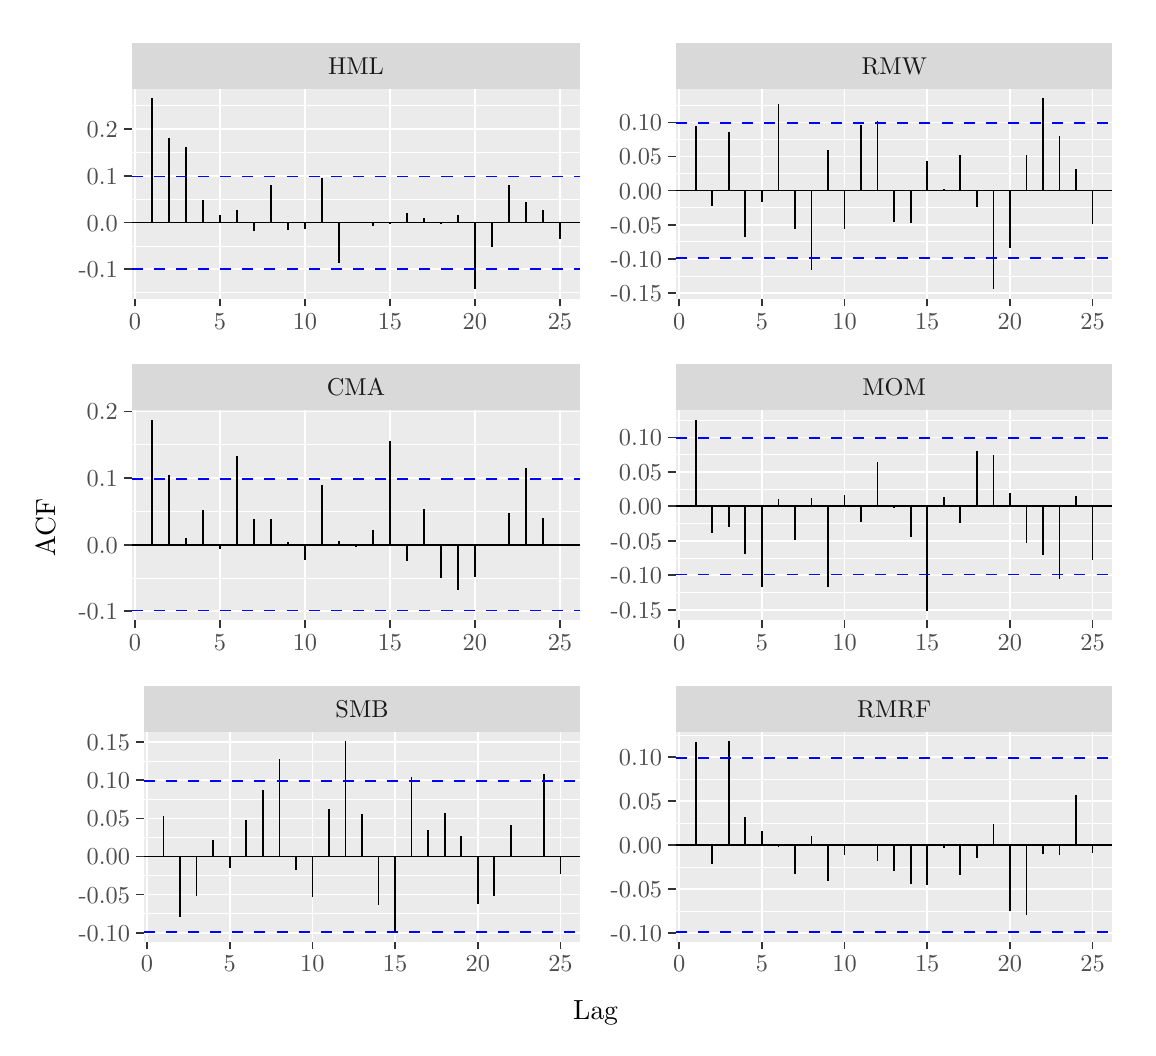
\begin{tikzpicture}[x=1pt,y=1pt]
\definecolor{fillColor}{RGB}{255,255,255}
\path[use as bounding box,fill=fillColor,fill opacity=0.00] (0,0) rectangle (397.48,361.35);
\begin{scope}
\path[clip] ( 12.91,245.20) rectangle (205.20,361.35);
\definecolor{drawColor}{RGB}{255,255,255}
\definecolor{fillColor}{RGB}{255,255,255}

\path[draw=drawColor,line width= 0.6pt,line join=round,line cap=round,fill=fillColor] ( 12.91,245.20) rectangle (205.20,361.35);
\end{scope}
\begin{scope}
\path[clip] ( 37.53,263.42) rectangle (199.70,339.28);
\definecolor{fillColor}{gray}{0.92}

\path[fill=fillColor] ( 37.53,263.42) rectangle (199.70,339.28);
\definecolor{drawColor}{RGB}{255,255,255}

\path[draw=drawColor,line width= 0.3pt,line join=round] ( 37.53,265.60) --
	(199.70,265.60);

\path[draw=drawColor,line width= 0.3pt,line join=round] ( 37.53,282.47) --
	(199.70,282.47);

\path[draw=drawColor,line width= 0.3pt,line join=round] ( 37.53,299.34) --
	(199.70,299.34);

\path[draw=drawColor,line width= 0.3pt,line join=round] ( 37.53,316.21) --
	(199.70,316.21);

\path[draw=drawColor,line width= 0.3pt,line join=round] ( 37.53,333.08) --
	(199.70,333.08);

\path[draw=drawColor,line width= 0.6pt,line join=round] ( 37.53,274.03) --
	(199.70,274.03);

\path[draw=drawColor,line width= 0.6pt,line join=round] ( 37.53,290.90) --
	(199.70,290.90);

\path[draw=drawColor,line width= 0.6pt,line join=round] ( 37.53,307.77) --
	(199.70,307.77);

\path[draw=drawColor,line width= 0.6pt,line join=round] ( 37.53,324.64) --
	(199.70,324.64);

\path[draw=drawColor,line width= 0.6pt,line join=round] ( 38.76,263.42) --
	( 38.76,339.28);

\path[draw=drawColor,line width= 0.6pt,line join=round] ( 69.48,263.42) --
	( 69.48,339.28);

\path[draw=drawColor,line width= 0.6pt,line join=round] (100.19,263.42) --
	(100.19,339.28);

\path[draw=drawColor,line width= 0.6pt,line join=round] (130.90,263.42) --
	(130.90,339.28);

\path[draw=drawColor,line width= 0.6pt,line join=round] (161.61,263.42) --
	(161.61,339.28);

\path[draw=drawColor,line width= 0.6pt,line join=round] (192.33,263.42) --
	(192.33,339.28);
\definecolor{drawColor}{RGB}{0,0,0}

\path[draw=drawColor,line width= 0.6pt,line join=round] ( 37.53,290.90) -- (199.70,290.90);

\path[draw=drawColor,line width= 0.6pt,line join=round] ( 44.91,290.90) -- ( 44.91,335.83);

\path[draw=drawColor,line width= 0.6pt,line join=round] ( 51.05,290.90) -- ( 51.05,321.49);

\path[draw=drawColor,line width= 0.6pt,line join=round] ( 57.19,290.90) -- ( 57.19,318.10);

\path[draw=drawColor,line width= 0.6pt,line join=round] ( 63.33,290.90) -- ( 63.33,299.08);

\path[draw=drawColor,line width= 0.6pt,line join=round] ( 69.48,290.90) -- ( 69.48,293.55);

\path[draw=drawColor,line width= 0.6pt,line join=round] ( 75.62,290.90) -- ( 75.62,295.48);

\path[draw=drawColor,line width= 0.6pt,line join=round] ( 81.76,290.90) -- ( 81.76,287.70);

\path[draw=drawColor,line width= 0.6pt,line join=round] ( 87.90,290.90) -- ( 87.90,304.48);

\path[draw=drawColor,line width= 0.6pt,line join=round] ( 94.05,290.90) -- ( 94.05,288.06);

\path[draw=drawColor,line width= 0.6pt,line join=round] (100.19,290.90) -- (100.19,288.60);

\path[draw=drawColor,line width= 0.6pt,line join=round] (106.33,290.90) -- (106.33,307.12);

\path[draw=drawColor,line width= 0.6pt,line join=round] (112.47,290.90) -- (112.47,276.32);

\path[draw=drawColor,line width= 0.6pt,line join=round] (118.62,290.90) -- (118.62,291.24);

\path[draw=drawColor,line width= 0.6pt,line join=round] (124.76,290.90) -- (124.76,289.66);

\path[draw=drawColor,line width= 0.6pt,line join=round] (130.90,290.90) -- (130.90,290.23);

\path[draw=drawColor,line width= 0.6pt,line join=round] (137.04,290.90) -- (137.04,294.36);

\path[draw=drawColor,line width= 0.6pt,line join=round] (143.19,290.90) -- (143.19,292.53);

\path[draw=drawColor,line width= 0.6pt,line join=round] (149.33,290.90) -- (149.33,290.23);

\path[draw=drawColor,line width= 0.6pt,line join=round] (155.47,290.90) -- (155.47,293.65);

\path[draw=drawColor,line width= 0.6pt,line join=round] (161.61,290.90) -- (161.61,266.87);

\path[draw=drawColor,line width= 0.6pt,line join=round] (167.76,290.90) -- (167.76,281.99);

\path[draw=drawColor,line width= 0.6pt,line join=round] (173.90,290.90) -- (173.90,304.52);

\path[draw=drawColor,line width= 0.6pt,line join=round] (180.04,290.90) -- (180.04,298.22);

\path[draw=drawColor,line width= 0.6pt,line join=round] (186.18,290.90) -- (186.18,295.41);

\path[draw=drawColor,line width= 0.6pt,line join=round] (192.33,290.90) -- (192.33,284.82);
\definecolor{drawColor}{RGB}{0,0,255}

\path[draw=drawColor,line width= 0.6pt,dash pattern=on 4pt off 4pt ,line join=round] ( 37.53,274.22) -- (199.70,274.22);

\path[draw=drawColor,line width= 0.6pt,dash pattern=on 4pt off 4pt ,line join=round] ( 37.53,307.58) -- (199.70,307.58);
\end{scope}
\begin{scope}
\path[clip] ( 37.53,339.28) rectangle (199.70,355.85);
\definecolor{fillColor}{gray}{0.85}

\path[fill=fillColor] ( 37.53,339.28) rectangle (199.70,355.85);
\definecolor{drawColor}{gray}{0.10}

\node[text=drawColor,anchor=base,inner sep=0pt, outer sep=0pt, scale=  0.88] at (118.62,344.53) {HML};
\end{scope}
\begin{scope}
\path[clip] (  0.00,  0.00) rectangle (397.48,361.35);
\definecolor{drawColor}{gray}{0.20}

\path[draw=drawColor,line width= 0.6pt,line join=round] ( 38.76,260.67) --
	( 38.76,263.42);

\path[draw=drawColor,line width= 0.6pt,line join=round] ( 69.48,260.67) --
	( 69.48,263.42);

\path[draw=drawColor,line width= 0.6pt,line join=round] (100.19,260.67) --
	(100.19,263.42);

\path[draw=drawColor,line width= 0.6pt,line join=round] (130.90,260.67) --
	(130.90,263.42);

\path[draw=drawColor,line width= 0.6pt,line join=round] (161.61,260.67) --
	(161.61,263.42);

\path[draw=drawColor,line width= 0.6pt,line join=round] (192.33,260.67) --
	(192.33,263.42);
\end{scope}
\begin{scope}
\path[clip] (  0.00,  0.00) rectangle (397.48,361.35);
\definecolor{drawColor}{gray}{0.30}

\node[text=drawColor,anchor=base,inner sep=0pt, outer sep=0pt, scale=  0.88] at ( 38.76,252.41) {0};

\node[text=drawColor,anchor=base,inner sep=0pt, outer sep=0pt, scale=  0.88] at ( 69.48,252.41) {5};

\node[text=drawColor,anchor=base,inner sep=0pt, outer sep=0pt, scale=  0.88] at (100.19,252.41) {10};

\node[text=drawColor,anchor=base,inner sep=0pt, outer sep=0pt, scale=  0.88] at (130.90,252.41) {15};

\node[text=drawColor,anchor=base,inner sep=0pt, outer sep=0pt, scale=  0.88] at (161.61,252.41) {20};

\node[text=drawColor,anchor=base,inner sep=0pt, outer sep=0pt, scale=  0.88] at (192.33,252.41) {25};
\end{scope}
\begin{scope}
\path[clip] (  0.00,  0.00) rectangle (397.48,361.35);
\definecolor{drawColor}{gray}{0.30}

\node[text=drawColor,anchor=base east,inner sep=0pt, outer sep=0pt, scale=  0.88] at ( 32.58,271.00) {-0.1};

\node[text=drawColor,anchor=base east,inner sep=0pt, outer sep=0pt, scale=  0.88] at ( 32.58,287.87) {0.0};

\node[text=drawColor,anchor=base east,inner sep=0pt, outer sep=0pt, scale=  0.88] at ( 32.58,304.74) {0.1};

\node[text=drawColor,anchor=base east,inner sep=0pt, outer sep=0pt, scale=  0.88] at ( 32.58,321.61) {0.2};
\end{scope}
\begin{scope}
\path[clip] (  0.00,  0.00) rectangle (397.48,361.35);
\definecolor{drawColor}{gray}{0.20}

\path[draw=drawColor,line width= 0.6pt,line join=round] ( 34.78,274.03) --
	( 37.53,274.03);

\path[draw=drawColor,line width= 0.6pt,line join=round] ( 34.78,290.90) --
	( 37.53,290.90);

\path[draw=drawColor,line width= 0.6pt,line join=round] ( 34.78,307.77) --
	( 37.53,307.77);

\path[draw=drawColor,line width= 0.6pt,line join=round] ( 34.78,324.64) --
	( 37.53,324.64);
\end{scope}
\begin{scope}
\path[clip] (205.20,245.20) rectangle (397.48,361.35);
\definecolor{drawColor}{RGB}{255,255,255}
\definecolor{fillColor}{RGB}{255,255,255}

\path[draw=drawColor,line width= 0.6pt,line join=round,line cap=round,fill=fillColor] (205.20,245.20) rectangle (397.48,361.35);
\end{scope}
\begin{scope}
\path[clip] (234.22,263.42) rectangle (391.98,339.28);
\definecolor{fillColor}{gray}{0.92}

\path[fill=fillColor] (234.22,263.42) rectangle (391.98,339.28);
\definecolor{drawColor}{RGB}{255,255,255}

\path[draw=drawColor,line width= 0.3pt,line join=round] (234.22,271.64) --
	(391.98,271.64);

\path[draw=drawColor,line width= 0.3pt,line join=round] (234.22,283.97) --
	(391.98,283.97);

\path[draw=drawColor,line width= 0.3pt,line join=round] (234.22,296.29) --
	(391.98,296.29);

\path[draw=drawColor,line width= 0.3pt,line join=round] (234.22,308.62) --
	(391.98,308.62);

\path[draw=drawColor,line width= 0.3pt,line join=round] (234.22,320.94) --
	(391.98,320.94);

\path[draw=drawColor,line width= 0.3pt,line join=round] (234.22,333.27) --
	(391.98,333.27);

\path[draw=drawColor,line width= 0.6pt,line join=round] (234.22,265.48) --
	(391.98,265.48);

\path[draw=drawColor,line width= 0.6pt,line join=round] (234.22,277.80) --
	(391.98,277.80);

\path[draw=drawColor,line width= 0.6pt,line join=round] (234.22,290.13) --
	(391.98,290.13);

\path[draw=drawColor,line width= 0.6pt,line join=round] (234.22,302.46) --
	(391.98,302.46);

\path[draw=drawColor,line width= 0.6pt,line join=round] (234.22,314.78) --
	(391.98,314.78);

\path[draw=drawColor,line width= 0.6pt,line join=round] (234.22,327.11) --
	(391.98,327.11);

\path[draw=drawColor,line width= 0.6pt,line join=round] (235.42,263.42) --
	(235.42,339.28);

\path[draw=drawColor,line width= 0.6pt,line join=round] (265.30,263.42) --
	(265.30,339.28);

\path[draw=drawColor,line width= 0.6pt,line join=round] (295.18,263.42) --
	(295.18,339.28);

\path[draw=drawColor,line width= 0.6pt,line join=round] (325.05,263.42) --
	(325.05,339.28);

\path[draw=drawColor,line width= 0.6pt,line join=round] (354.93,263.42) --
	(354.93,339.28);

\path[draw=drawColor,line width= 0.6pt,line join=round] (384.81,263.42) --
	(384.81,339.28);
\definecolor{drawColor}{RGB}{0,0,0}

\path[draw=drawColor,line width= 0.6pt,line join=round] (234.22,302.46) -- (391.98,302.46);

\path[draw=drawColor,line width= 0.6pt,line join=round] (241.39,302.46) -- (241.39,325.99);

\path[draw=drawColor,line width= 0.6pt,line join=round] (247.37,302.46) -- (247.37,296.86);

\path[draw=drawColor,line width= 0.6pt,line join=round] (253.34,302.46) -- (253.34,323.74);

\path[draw=drawColor,line width= 0.6pt,line join=round] (259.32,302.46) -- (259.32,285.78);

\path[draw=drawColor,line width= 0.6pt,line join=round] (265.30,302.46) -- (265.30,298.36);

\path[draw=drawColor,line width= 0.6pt,line join=round] (271.27,302.46) -- (271.27,333.59);

\path[draw=drawColor,line width= 0.6pt,line join=round] (277.25,302.46) -- (277.25,288.76);

\path[draw=drawColor,line width= 0.6pt,line join=round] (283.22,302.46) -- (283.22,273.76);

\path[draw=drawColor,line width= 0.6pt,line join=round] (289.20,302.46) -- (289.20,317.10);

\path[draw=drawColor,line width= 0.6pt,line join=round] (295.18,302.46) -- (295.18,288.64);

\path[draw=drawColor,line width= 0.6pt,line join=round] (301.15,302.46) -- (301.15,326.00);

\path[draw=drawColor,line width= 0.6pt,line join=round] (307.13,302.46) -- (307.13,327.77);

\path[draw=drawColor,line width= 0.6pt,line join=round] (313.10,302.46) -- (313.10,291.11);

\path[draw=drawColor,line width= 0.6pt,line join=round] (319.08,302.46) -- (319.08,290.89);

\path[draw=drawColor,line width= 0.6pt,line join=round] (325.05,302.46) -- (325.05,313.15);

\path[draw=drawColor,line width= 0.6pt,line join=round] (331.03,302.46) -- (331.03,303.15);

\path[draw=drawColor,line width= 0.6pt,line join=round] (337.01,302.46) -- (337.01,315.32);

\path[draw=drawColor,line width= 0.6pt,line join=round] (342.98,302.46) -- (342.98,296.53);

\path[draw=drawColor,line width= 0.6pt,line join=round] (348.96,302.46) -- (348.96,266.87);

\path[draw=drawColor,line width= 0.6pt,line join=round] (354.93,302.46) -- (354.93,281.58);

\path[draw=drawColor,line width= 0.6pt,line join=round] (360.91,302.46) -- (360.91,315.46);

\path[draw=drawColor,line width= 0.6pt,line join=round] (366.89,302.46) -- (366.89,335.83);

\path[draw=drawColor,line width= 0.6pt,line join=round] (372.86,302.46) -- (372.86,322.16);

\path[draw=drawColor,line width= 0.6pt,line join=round] (378.84,302.46) -- (378.84,310.37);

\path[draw=drawColor,line width= 0.6pt,line join=round] (384.81,302.46) -- (384.81,290.56);
\definecolor{drawColor}{RGB}{0,0,255}

\path[draw=drawColor,line width= 0.6pt,dash pattern=on 4pt off 4pt ,line join=round] (234.22,278.08) -- (391.98,278.08);

\path[draw=drawColor,line width= 0.6pt,dash pattern=on 4pt off 4pt ,line join=round] (234.22,326.83) -- (391.98,326.83);
\end{scope}
\begin{scope}
\path[clip] (234.22,339.28) rectangle (391.98,355.85);
\definecolor{fillColor}{gray}{0.85}

\path[fill=fillColor] (234.22,339.28) rectangle (391.98,355.85);
\definecolor{drawColor}{gray}{0.10}

\node[text=drawColor,anchor=base,inner sep=0pt, outer sep=0pt, scale=  0.88] at (313.10,344.53) {RMW};
\end{scope}
\begin{scope}
\path[clip] (  0.00,  0.00) rectangle (397.48,361.35);
\definecolor{drawColor}{gray}{0.20}

\path[draw=drawColor,line width= 0.6pt,line join=round] (235.42,260.67) --
	(235.42,263.42);

\path[draw=drawColor,line width= 0.6pt,line join=round] (265.30,260.67) --
	(265.30,263.42);

\path[draw=drawColor,line width= 0.6pt,line join=round] (295.18,260.67) --
	(295.18,263.42);

\path[draw=drawColor,line width= 0.6pt,line join=round] (325.05,260.67) --
	(325.05,263.42);

\path[draw=drawColor,line width= 0.6pt,line join=round] (354.93,260.67) --
	(354.93,263.42);

\path[draw=drawColor,line width= 0.6pt,line join=round] (384.81,260.67) --
	(384.81,263.42);
\end{scope}
\begin{scope}
\path[clip] (  0.00,  0.00) rectangle (397.48,361.35);
\definecolor{drawColor}{gray}{0.30}

\node[text=drawColor,anchor=base,inner sep=0pt, outer sep=0pt, scale=  0.88] at (235.42,252.41) {0};

\node[text=drawColor,anchor=base,inner sep=0pt, outer sep=0pt, scale=  0.88] at (265.30,252.41) {5};

\node[text=drawColor,anchor=base,inner sep=0pt, outer sep=0pt, scale=  0.88] at (295.18,252.41) {10};

\node[text=drawColor,anchor=base,inner sep=0pt, outer sep=0pt, scale=  0.88] at (325.05,252.41) {15};

\node[text=drawColor,anchor=base,inner sep=0pt, outer sep=0pt, scale=  0.88] at (354.93,252.41) {20};

\node[text=drawColor,anchor=base,inner sep=0pt, outer sep=0pt, scale=  0.88] at (384.81,252.41) {25};
\end{scope}
\begin{scope}
\path[clip] (  0.00,  0.00) rectangle (397.48,361.35);
\definecolor{drawColor}{gray}{0.30}

\node[text=drawColor,anchor=base east,inner sep=0pt, outer sep=0pt, scale=  0.88] at (229.27,262.45) {-0.15};

\node[text=drawColor,anchor=base east,inner sep=0pt, outer sep=0pt, scale=  0.88] at (229.27,274.77) {-0.10};

\node[text=drawColor,anchor=base east,inner sep=0pt, outer sep=0pt, scale=  0.88] at (229.27,287.10) {-0.05};

\node[text=drawColor,anchor=base east,inner sep=0pt, outer sep=0pt, scale=  0.88] at (229.27,299.42) {0.00};

\node[text=drawColor,anchor=base east,inner sep=0pt, outer sep=0pt, scale=  0.88] at (229.27,311.75) {0.05};

\node[text=drawColor,anchor=base east,inner sep=0pt, outer sep=0pt, scale=  0.88] at (229.27,324.08) {0.10};
\end{scope}
\begin{scope}
\path[clip] (  0.00,  0.00) rectangle (397.48,361.35);
\definecolor{drawColor}{gray}{0.20}

\path[draw=drawColor,line width= 0.6pt,line join=round] (231.47,265.48) --
	(234.22,265.48);

\path[draw=drawColor,line width= 0.6pt,line join=round] (231.47,277.80) --
	(234.22,277.80);

\path[draw=drawColor,line width= 0.6pt,line join=round] (231.47,290.13) --
	(234.22,290.13);

\path[draw=drawColor,line width= 0.6pt,line join=round] (231.47,302.46) --
	(234.22,302.46);

\path[draw=drawColor,line width= 0.6pt,line join=round] (231.47,314.78) --
	(234.22,314.78);

\path[draw=drawColor,line width= 0.6pt,line join=round] (231.47,327.11) --
	(234.22,327.11);
\end{scope}
\begin{scope}
\path[clip] ( 12.91,129.06) rectangle (205.20,245.20);
\definecolor{drawColor}{RGB}{255,255,255}
\definecolor{fillColor}{RGB}{255,255,255}

\path[draw=drawColor,line width= 0.6pt,line join=round,line cap=round,fill=fillColor] ( 12.91,129.06) rectangle (205.20,245.20);
\end{scope}
\begin{scope}
\path[clip] ( 37.53,147.28) rectangle (199.70,223.13);
\definecolor{fillColor}{gray}{0.92}

\path[fill=fillColor] ( 37.53,147.28) rectangle (199.70,223.13);
\definecolor{drawColor}{RGB}{255,255,255}

\path[draw=drawColor,line width= 0.3pt,line join=round] ( 37.53,162.49) --
	(199.70,162.49);

\path[draw=drawColor,line width= 0.3pt,line join=round] ( 37.53,186.57) --
	(199.70,186.57);

\path[draw=drawColor,line width= 0.3pt,line join=round] ( 37.53,210.65) --
	(199.70,210.65);

\path[draw=drawColor,line width= 0.6pt,line join=round] ( 37.53,150.45) --
	(199.70,150.45);

\path[draw=drawColor,line width= 0.6pt,line join=round] ( 37.53,174.53) --
	(199.70,174.53);

\path[draw=drawColor,line width= 0.6pt,line join=round] ( 37.53,198.61) --
	(199.70,198.61);

\path[draw=drawColor,line width= 0.6pt,line join=round] ( 37.53,222.68) --
	(199.70,222.68);

\path[draw=drawColor,line width= 0.6pt,line join=round] ( 38.76,147.28) --
	( 38.76,223.13);

\path[draw=drawColor,line width= 0.6pt,line join=round] ( 69.48,147.28) --
	( 69.48,223.13);

\path[draw=drawColor,line width= 0.6pt,line join=round] (100.19,147.28) --
	(100.19,223.13);

\path[draw=drawColor,line width= 0.6pt,line join=round] (130.90,147.28) --
	(130.90,223.13);

\path[draw=drawColor,line width= 0.6pt,line join=round] (161.61,147.28) --
	(161.61,223.13);

\path[draw=drawColor,line width= 0.6pt,line join=round] (192.33,147.28) --
	(192.33,223.13);
\definecolor{drawColor}{RGB}{0,0,0}

\path[draw=drawColor,line width= 0.6pt,line join=round] ( 37.53,174.53) -- (199.70,174.53);

\path[draw=drawColor,line width= 0.6pt,line join=round] ( 44.91,174.53) -- ( 44.91,219.68);

\path[draw=drawColor,line width= 0.6pt,line join=round] ( 51.05,174.53) -- ( 51.05,199.77);

\path[draw=drawColor,line width= 0.6pt,line join=round] ( 57.19,174.53) -- ( 57.19,177.12);

\path[draw=drawColor,line width= 0.6pt,line join=round] ( 63.33,174.53) -- ( 63.33,187.08);

\path[draw=drawColor,line width= 0.6pt,line join=round] ( 69.48,174.53) -- ( 69.48,173.10);

\path[draw=drawColor,line width= 0.6pt,line join=round] ( 75.62,174.53) -- ( 75.62,206.74);

\path[draw=drawColor,line width= 0.6pt,line join=round] ( 81.76,174.53) -- ( 81.76,183.67);

\path[draw=drawColor,line width= 0.6pt,line join=round] ( 87.90,174.53) -- ( 87.90,183.64);

\path[draw=drawColor,line width= 0.6pt,line join=round] ( 94.05,174.53) -- ( 94.05,175.46);

\path[draw=drawColor,line width= 0.6pt,line join=round] (100.19,174.53) -- (100.19,168.87);

\path[draw=drawColor,line width= 0.6pt,line join=round] (106.33,174.53) -- (106.33,196.01);

\path[draw=drawColor,line width= 0.6pt,line join=round] (112.47,174.53) -- (112.47,175.73);

\path[draw=drawColor,line width= 0.6pt,line join=round] (118.62,174.53) -- (118.62,173.69);

\path[draw=drawColor,line width= 0.6pt,line join=round] (124.76,174.53) -- (124.76,179.90);

\path[draw=drawColor,line width= 0.6pt,line join=round] (130.90,174.53) -- (130.90,211.86);

\path[draw=drawColor,line width= 0.6pt,line join=round] (137.04,174.53) -- (137.04,168.52);

\path[draw=drawColor,line width= 0.6pt,line join=round] (143.19,174.53) -- (143.19,187.31);

\path[draw=drawColor,line width= 0.6pt,line join=round] (149.33,174.53) -- (149.33,162.62);

\path[draw=drawColor,line width= 0.6pt,line join=round] (155.47,174.53) -- (155.47,158.12);

\path[draw=drawColor,line width= 0.6pt,line join=round] (161.61,174.53) -- (161.61,162.93);

\path[draw=drawColor,line width= 0.6pt,line join=round] (167.76,174.53) -- (167.76,174.25);

\path[draw=drawColor,line width= 0.6pt,line join=round] (173.90,174.53) -- (173.90,185.98);

\path[draw=drawColor,line width= 0.6pt,line join=round] (180.04,174.53) -- (180.04,202.32);

\path[draw=drawColor,line width= 0.6pt,line join=round] (186.18,174.53) -- (186.18,184.23);

\path[draw=drawColor,line width= 0.6pt,line join=round] (192.33,174.53) -- (192.33,174.24);
\definecolor{drawColor}{RGB}{0,0,255}

\path[draw=drawColor,line width= 0.6pt,dash pattern=on 4pt off 4pt ,line join=round] ( 37.53,150.73) -- (199.70,150.73);

\path[draw=drawColor,line width= 0.6pt,dash pattern=on 4pt off 4pt ,line join=round] ( 37.53,198.33) -- (199.70,198.33);
\end{scope}
\begin{scope}
\path[clip] ( 37.53,223.13) rectangle (199.70,239.70);
\definecolor{fillColor}{gray}{0.85}

\path[fill=fillColor] ( 37.53,223.13) rectangle (199.70,239.70);
\definecolor{drawColor}{gray}{0.10}

\node[text=drawColor,anchor=base,inner sep=0pt, outer sep=0pt, scale=  0.88] at (118.62,228.39) {CMA};
\end{scope}
\begin{scope}
\path[clip] (  0.00,  0.00) rectangle (397.48,361.35);
\definecolor{drawColor}{gray}{0.20}

\path[draw=drawColor,line width= 0.6pt,line join=round] ( 38.76,144.53) --
	( 38.76,147.28);

\path[draw=drawColor,line width= 0.6pt,line join=round] ( 69.48,144.53) --
	( 69.48,147.28);

\path[draw=drawColor,line width= 0.6pt,line join=round] (100.19,144.53) --
	(100.19,147.28);

\path[draw=drawColor,line width= 0.6pt,line join=round] (130.90,144.53) --
	(130.90,147.28);

\path[draw=drawColor,line width= 0.6pt,line join=round] (161.61,144.53) --
	(161.61,147.28);

\path[draw=drawColor,line width= 0.6pt,line join=round] (192.33,144.53) --
	(192.33,147.28);
\end{scope}
\begin{scope}
\path[clip] (  0.00,  0.00) rectangle (397.48,361.35);
\definecolor{drawColor}{gray}{0.30}

\node[text=drawColor,anchor=base,inner sep=0pt, outer sep=0pt, scale=  0.88] at ( 38.76,136.27) {0};

\node[text=drawColor,anchor=base,inner sep=0pt, outer sep=0pt, scale=  0.88] at ( 69.48,136.27) {5};

\node[text=drawColor,anchor=base,inner sep=0pt, outer sep=0pt, scale=  0.88] at (100.19,136.27) {10};

\node[text=drawColor,anchor=base,inner sep=0pt, outer sep=0pt, scale=  0.88] at (130.90,136.27) {15};

\node[text=drawColor,anchor=base,inner sep=0pt, outer sep=0pt, scale=  0.88] at (161.61,136.27) {20};

\node[text=drawColor,anchor=base,inner sep=0pt, outer sep=0pt, scale=  0.88] at (192.33,136.27) {25};
\end{scope}
\begin{scope}
\path[clip] (  0.00,  0.00) rectangle (397.48,361.35);
\definecolor{drawColor}{gray}{0.30}

\node[text=drawColor,anchor=base east,inner sep=0pt, outer sep=0pt, scale=  0.88] at ( 32.58,147.42) {-0.1};

\node[text=drawColor,anchor=base east,inner sep=0pt, outer sep=0pt, scale=  0.88] at ( 32.58,171.50) {0.0};

\node[text=drawColor,anchor=base east,inner sep=0pt, outer sep=0pt, scale=  0.88] at ( 32.58,195.58) {0.1};

\node[text=drawColor,anchor=base east,inner sep=0pt, outer sep=0pt, scale=  0.88] at ( 32.58,219.65) {0.2};
\end{scope}
\begin{scope}
\path[clip] (  0.00,  0.00) rectangle (397.48,361.35);
\definecolor{drawColor}{gray}{0.20}

\path[draw=drawColor,line width= 0.6pt,line join=round] ( 34.78,150.45) --
	( 37.53,150.45);

\path[draw=drawColor,line width= 0.6pt,line join=round] ( 34.78,174.53) --
	( 37.53,174.53);

\path[draw=drawColor,line width= 0.6pt,line join=round] ( 34.78,198.61) --
	( 37.53,198.61);

\path[draw=drawColor,line width= 0.6pt,line join=round] ( 34.78,222.68) --
	( 37.53,222.68);
\end{scope}
\begin{scope}
\path[clip] (205.20,129.06) rectangle (397.48,245.20);
\definecolor{drawColor}{RGB}{255,255,255}
\definecolor{fillColor}{RGB}{255,255,255}

\path[draw=drawColor,line width= 0.6pt,line join=round,line cap=round,fill=fillColor] (205.20,129.06) rectangle (397.48,245.20);
\end{scope}
\begin{scope}
\path[clip] (234.22,147.28) rectangle (391.98,223.13);
\definecolor{fillColor}{gray}{0.92}

\path[fill=fillColor] (234.22,147.28) rectangle (391.98,223.13);
\definecolor{drawColor}{RGB}{255,255,255}

\path[draw=drawColor,line width= 0.3pt,line join=round] (234.22,157.27) --
	(391.98,157.27);

\path[draw=drawColor,line width= 0.3pt,line join=round] (234.22,169.72) --
	(391.98,169.72);

\path[draw=drawColor,line width= 0.3pt,line join=round] (234.22,182.17) --
	(391.98,182.17);

\path[draw=drawColor,line width= 0.3pt,line join=round] (234.22,194.62) --
	(391.98,194.62);

\path[draw=drawColor,line width= 0.3pt,line join=round] (234.22,207.07) --
	(391.98,207.07);

\path[draw=drawColor,line width= 0.3pt,line join=round] (234.22,219.52) --
	(391.98,219.52);

\path[draw=drawColor,line width= 0.6pt,line join=round] (234.22,151.04) --
	(391.98,151.04);

\path[draw=drawColor,line width= 0.6pt,line join=round] (234.22,163.49) --
	(391.98,163.49);

\path[draw=drawColor,line width= 0.6pt,line join=round] (234.22,175.94) --
	(391.98,175.94);

\path[draw=drawColor,line width= 0.6pt,line join=round] (234.22,188.39) --
	(391.98,188.39);

\path[draw=drawColor,line width= 0.6pt,line join=round] (234.22,200.84) --
	(391.98,200.84);

\path[draw=drawColor,line width= 0.6pt,line join=round] (234.22,213.29) --
	(391.98,213.29);

\path[draw=drawColor,line width= 0.6pt,line join=round] (235.42,147.28) --
	(235.42,223.13);

\path[draw=drawColor,line width= 0.6pt,line join=round] (265.30,147.28) --
	(265.30,223.13);

\path[draw=drawColor,line width= 0.6pt,line join=round] (295.18,147.28) --
	(295.18,223.13);

\path[draw=drawColor,line width= 0.6pt,line join=round] (325.05,147.28) --
	(325.05,223.13);

\path[draw=drawColor,line width= 0.6pt,line join=round] (354.93,147.28) --
	(354.93,223.13);

\path[draw=drawColor,line width= 0.6pt,line join=round] (384.81,147.28) --
	(384.81,223.13);
\definecolor{drawColor}{RGB}{0,0,0}

\path[draw=drawColor,line width= 0.6pt,line join=round] (234.22,188.39) -- (391.98,188.39);

\path[draw=drawColor,line width= 0.6pt,line join=round] (241.39,188.39) -- (241.39,219.68);

\path[draw=drawColor,line width= 0.6pt,line join=round] (247.37,188.39) -- (247.37,178.60);

\path[draw=drawColor,line width= 0.6pt,line join=round] (253.34,188.39) -- (253.34,180.99);

\path[draw=drawColor,line width= 0.6pt,line join=round] (259.32,188.39) -- (259.32,171.13);

\path[draw=drawColor,line width= 0.6pt,line join=round] (265.30,188.39) -- (265.30,159.34);

\path[draw=drawColor,line width= 0.6pt,line join=round] (271.27,188.39) -- (271.27,190.92);

\path[draw=drawColor,line width= 0.6pt,line join=round] (277.25,188.39) -- (277.25,176.08);

\path[draw=drawColor,line width= 0.6pt,line join=round] (283.22,188.39) -- (283.22,191.49);

\path[draw=drawColor,line width= 0.6pt,line join=round] (289.20,188.39) -- (289.20,159.09);

\path[draw=drawColor,line width= 0.6pt,line join=round] (295.18,188.39) -- (295.18,192.59);

\path[draw=drawColor,line width= 0.6pt,line join=round] (301.15,188.39) -- (301.15,182.69);

\path[draw=drawColor,line width= 0.6pt,line join=round] (307.13,188.39) -- (307.13,204.24);

\path[draw=drawColor,line width= 0.6pt,line join=round] (313.10,188.39) -- (313.10,187.74);

\path[draw=drawColor,line width= 0.6pt,line join=round] (319.08,188.39) -- (319.08,177.20);

\path[draw=drawColor,line width= 0.6pt,line join=round] (325.05,188.39) -- (325.05,150.73);

\path[draw=drawColor,line width= 0.6pt,line join=round] (331.03,188.39) -- (331.03,191.77);

\path[draw=drawColor,line width= 0.6pt,line join=round] (337.01,188.39) -- (337.01,182.29);

\path[draw=drawColor,line width= 0.6pt,line join=round] (342.98,188.39) -- (342.98,208.47);

\path[draw=drawColor,line width= 0.6pt,line join=round] (348.96,188.39) -- (348.96,206.82);

\path[draw=drawColor,line width= 0.6pt,line join=round] (354.93,188.39) -- (354.93,193.24);

\path[draw=drawColor,line width= 0.6pt,line join=round] (360.91,188.39) -- (360.91,175.18);

\path[draw=drawColor,line width= 0.6pt,line join=round] (366.89,188.39) -- (366.89,170.87);

\path[draw=drawColor,line width= 0.6pt,line join=round] (372.86,188.39) -- (372.86,162.02);

\path[draw=drawColor,line width= 0.6pt,line join=round] (378.84,188.39) -- (378.84,192.15);

\path[draw=drawColor,line width= 0.6pt,line join=round] (384.81,188.39) -- (384.81,168.93);
\definecolor{drawColor}{RGB}{0,0,255}

\path[draw=drawColor,line width= 0.6pt,dash pattern=on 4pt off 4pt ,line join=round] (234.22,163.77) -- (391.98,163.77);

\path[draw=drawColor,line width= 0.6pt,dash pattern=on 4pt off 4pt ,line join=round] (234.22,213.01) -- (391.98,213.01);
\end{scope}
\begin{scope}
\path[clip] (234.22,223.13) rectangle (391.98,239.70);
\definecolor{fillColor}{gray}{0.85}

\path[fill=fillColor] (234.22,223.13) rectangle (391.98,239.70);
\definecolor{drawColor}{gray}{0.10}

\node[text=drawColor,anchor=base,inner sep=0pt, outer sep=0pt, scale=  0.88] at (313.10,228.39) {MOM};
\end{scope}
\begin{scope}
\path[clip] (  0.00,  0.00) rectangle (397.48,361.35);
\definecolor{drawColor}{gray}{0.20}

\path[draw=drawColor,line width= 0.6pt,line join=round] (235.42,144.53) --
	(235.42,147.28);

\path[draw=drawColor,line width= 0.6pt,line join=round] (265.30,144.53) --
	(265.30,147.28);

\path[draw=drawColor,line width= 0.6pt,line join=round] (295.18,144.53) --
	(295.18,147.28);

\path[draw=drawColor,line width= 0.6pt,line join=round] (325.05,144.53) --
	(325.05,147.28);

\path[draw=drawColor,line width= 0.6pt,line join=round] (354.93,144.53) --
	(354.93,147.28);

\path[draw=drawColor,line width= 0.6pt,line join=round] (384.81,144.53) --
	(384.81,147.28);
\end{scope}
\begin{scope}
\path[clip] (  0.00,  0.00) rectangle (397.48,361.35);
\definecolor{drawColor}{gray}{0.30}

\node[text=drawColor,anchor=base,inner sep=0pt, outer sep=0pt, scale=  0.88] at (235.42,136.27) {0};

\node[text=drawColor,anchor=base,inner sep=0pt, outer sep=0pt, scale=  0.88] at (265.30,136.27) {5};

\node[text=drawColor,anchor=base,inner sep=0pt, outer sep=0pt, scale=  0.88] at (295.18,136.27) {10};

\node[text=drawColor,anchor=base,inner sep=0pt, outer sep=0pt, scale=  0.88] at (325.05,136.27) {15};

\node[text=drawColor,anchor=base,inner sep=0pt, outer sep=0pt, scale=  0.88] at (354.93,136.27) {20};

\node[text=drawColor,anchor=base,inner sep=0pt, outer sep=0pt, scale=  0.88] at (384.81,136.27) {25};
\end{scope}
\begin{scope}
\path[clip] (  0.00,  0.00) rectangle (397.48,361.35);
\definecolor{drawColor}{gray}{0.30}

\node[text=drawColor,anchor=base east,inner sep=0pt, outer sep=0pt, scale=  0.88] at (229.27,148.01) {-0.15};

\node[text=drawColor,anchor=base east,inner sep=0pt, outer sep=0pt, scale=  0.88] at (229.27,160.46) {-0.10};

\node[text=drawColor,anchor=base east,inner sep=0pt, outer sep=0pt, scale=  0.88] at (229.27,172.91) {-0.05};

\node[text=drawColor,anchor=base east,inner sep=0pt, outer sep=0pt, scale=  0.88] at (229.27,185.36) {0.00};

\node[text=drawColor,anchor=base east,inner sep=0pt, outer sep=0pt, scale=  0.88] at (229.27,197.81) {0.05};

\node[text=drawColor,anchor=base east,inner sep=0pt, outer sep=0pt, scale=  0.88] at (229.27,210.26) {0.10};
\end{scope}
\begin{scope}
\path[clip] (  0.00,  0.00) rectangle (397.48,361.35);
\definecolor{drawColor}{gray}{0.20}

\path[draw=drawColor,line width= 0.6pt,line join=round] (231.47,151.04) --
	(234.22,151.04);

\path[draw=drawColor,line width= 0.6pt,line join=round] (231.47,163.49) --
	(234.22,163.49);

\path[draw=drawColor,line width= 0.6pt,line join=round] (231.47,175.94) --
	(234.22,175.94);

\path[draw=drawColor,line width= 0.6pt,line join=round] (231.47,188.39) --
	(234.22,188.39);

\path[draw=drawColor,line width= 0.6pt,line join=round] (231.47,200.84) --
	(234.22,200.84);

\path[draw=drawColor,line width= 0.6pt,line join=round] (231.47,213.29) --
	(234.22,213.29);
\end{scope}
\begin{scope}
\path[clip] ( 12.91, 12.91) rectangle (205.20,129.06);
\definecolor{drawColor}{RGB}{255,255,255}
\definecolor{fillColor}{RGB}{255,255,255}

\path[draw=drawColor,line width= 0.6pt,line join=round,line cap=round,fill=fillColor] ( 12.91, 12.91) rectangle (205.20,129.06);
\end{scope}
\begin{scope}
\path[clip] ( 41.93, 31.13) rectangle (199.70,106.98);
\definecolor{fillColor}{gray}{0.92}

\path[fill=fillColor] ( 41.93, 31.13) rectangle (199.70,106.98);
\definecolor{drawColor}{RGB}{255,255,255}

\path[draw=drawColor,line width= 0.3pt,line join=round] ( 41.93, 41.16) --
	(199.70, 41.16);

\path[draw=drawColor,line width= 0.3pt,line join=round] ( 41.93, 54.95) --
	(199.70, 54.95);

\path[draw=drawColor,line width= 0.3pt,line join=round] ( 41.93, 68.75) --
	(199.70, 68.75);

\path[draw=drawColor,line width= 0.3pt,line join=round] ( 41.93, 82.54) --
	(199.70, 82.54);

\path[draw=drawColor,line width= 0.3pt,line join=round] ( 41.93, 96.33) --
	(199.70, 96.33);

\path[draw=drawColor,line width= 0.6pt,line join=round] ( 41.93, 34.27) --
	(199.70, 34.27);

\path[draw=drawColor,line width= 0.6pt,line join=round] ( 41.93, 48.06) --
	(199.70, 48.06);

\path[draw=drawColor,line width= 0.6pt,line join=round] ( 41.93, 61.85) --
	(199.70, 61.85);

\path[draw=drawColor,line width= 0.6pt,line join=round] ( 41.93, 75.64) --
	(199.70, 75.64);

\path[draw=drawColor,line width= 0.6pt,line join=round] ( 41.93, 89.43) --
	(199.70, 89.43);

\path[draw=drawColor,line width= 0.6pt,line join=round] ( 41.93,103.23) --
	(199.70,103.23);

\path[draw=drawColor,line width= 0.6pt,line join=round] ( 43.13, 31.13) --
	( 43.13,106.98);

\path[draw=drawColor,line width= 0.6pt,line join=round] ( 73.01, 31.13) --
	( 73.01,106.98);

\path[draw=drawColor,line width= 0.6pt,line join=round] (102.89, 31.13) --
	(102.89,106.98);

\path[draw=drawColor,line width= 0.6pt,line join=round] (132.77, 31.13) --
	(132.77,106.98);

\path[draw=drawColor,line width= 0.6pt,line join=round] (162.65, 31.13) --
	(162.65,106.98);

\path[draw=drawColor,line width= 0.6pt,line join=round] (192.53, 31.13) --
	(192.53,106.98);
\definecolor{drawColor}{RGB}{0,0,0}

\path[draw=drawColor,line width= 0.6pt,line join=round] ( 41.93, 61.85) -- (199.70, 61.85);

\path[draw=drawColor,line width= 0.6pt,line join=round] ( 49.10, 61.85) -- ( 49.10, 76.59);

\path[draw=drawColor,line width= 0.6pt,line join=round] ( 55.08, 61.85) -- ( 55.08, 39.83);

\path[draw=drawColor,line width= 0.6pt,line join=round] ( 61.06, 61.85) -- ( 61.06, 47.43);

\path[draw=drawColor,line width= 0.6pt,line join=round] ( 67.03, 61.85) -- ( 67.03, 67.78);

\path[draw=drawColor,line width= 0.6pt,line join=round] ( 73.01, 61.85) -- ( 73.01, 57.81);

\path[draw=drawColor,line width= 0.6pt,line join=round] ( 78.98, 61.85) -- ( 78.98, 75.05);

\path[draw=drawColor,line width= 0.6pt,line join=round] ( 84.96, 61.85) -- ( 84.96, 85.87);

\path[draw=drawColor,line width= 0.6pt,line join=round] ( 90.94, 61.85) -- ( 90.94, 97.26);

\path[draw=drawColor,line width= 0.6pt,line join=round] ( 96.91, 61.85) -- ( 96.91, 56.87);

\path[draw=drawColor,line width= 0.6pt,line join=round] (102.89, 61.85) -- (102.89, 47.26);

\path[draw=drawColor,line width= 0.6pt,line join=round] (108.86, 61.85) -- (108.86, 79.07);

\path[draw=drawColor,line width= 0.6pt,line join=round] (114.84, 61.85) -- (114.84,103.54);

\path[draw=drawColor,line width= 0.6pt,line join=round] (120.82, 61.85) -- (120.82, 77.08);

\path[draw=drawColor,line width= 0.6pt,line join=round] (126.79, 61.85) -- (126.79, 44.47);

\path[draw=drawColor,line width= 0.6pt,line join=round] (132.77, 61.85) -- (132.77, 35.10);

\path[draw=drawColor,line width= 0.6pt,line join=round] (138.74, 61.85) -- (138.74, 90.68);

\path[draw=drawColor,line width= 0.6pt,line join=round] (144.72, 61.85) -- (144.72, 71.46);

\path[draw=drawColor,line width= 0.6pt,line join=round] (150.69, 61.85) -- (150.69, 77.75);

\path[draw=drawColor,line width= 0.6pt,line join=round] (156.67, 61.85) -- (156.67, 69.38);

\path[draw=drawColor,line width= 0.6pt,line join=round] (162.65, 61.85) -- (162.65, 44.72);

\path[draw=drawColor,line width= 0.6pt,line join=round] (168.62, 61.85) -- (168.62, 47.74);

\path[draw=drawColor,line width= 0.6pt,line join=round] (174.60, 61.85) -- (174.60, 73.31);

\path[draw=drawColor,line width= 0.6pt,line join=round] (180.57, 61.85) -- (180.57, 61.97);

\path[draw=drawColor,line width= 0.6pt,line join=round] (186.55, 61.85) -- (186.55, 91.61);

\path[draw=drawColor,line width= 0.6pt,line join=round] (192.53, 61.85) -- (192.53, 55.57);
\definecolor{drawColor}{RGB}{0,0,255}

\path[draw=drawColor,line width= 0.6pt,dash pattern=on 4pt off 4pt ,line join=round] ( 41.93, 34.58) -- (199.70, 34.58);

\path[draw=drawColor,line width= 0.6pt,dash pattern=on 4pt off 4pt ,line join=round] ( 41.93, 89.12) -- (199.70, 89.12);
\end{scope}
\begin{scope}
\path[clip] ( 41.93,106.98) rectangle (199.70,123.56);
\definecolor{fillColor}{gray}{0.85}

\path[fill=fillColor] ( 41.93,106.98) rectangle (199.70,123.56);
\definecolor{drawColor}{gray}{0.10}

\node[text=drawColor,anchor=base,inner sep=0pt, outer sep=0pt, scale=  0.88] at (120.82,112.24) {SMB};
\end{scope}
\begin{scope}
\path[clip] (  0.00,  0.00) rectangle (397.48,361.35);
\definecolor{drawColor}{gray}{0.20}

\path[draw=drawColor,line width= 0.6pt,line join=round] ( 43.13, 28.38) --
	( 43.13, 31.13);

\path[draw=drawColor,line width= 0.6pt,line join=round] ( 73.01, 28.38) --
	( 73.01, 31.13);

\path[draw=drawColor,line width= 0.6pt,line join=round] (102.89, 28.38) --
	(102.89, 31.13);

\path[draw=drawColor,line width= 0.6pt,line join=round] (132.77, 28.38) --
	(132.77, 31.13);

\path[draw=drawColor,line width= 0.6pt,line join=round] (162.65, 28.38) --
	(162.65, 31.13);

\path[draw=drawColor,line width= 0.6pt,line join=round] (192.53, 28.38) --
	(192.53, 31.13);
\end{scope}
\begin{scope}
\path[clip] (  0.00,  0.00) rectangle (397.48,361.35);
\definecolor{drawColor}{gray}{0.30}

\node[text=drawColor,anchor=base,inner sep=0pt, outer sep=0pt, scale=  0.88] at ( 43.13, 20.12) {0};

\node[text=drawColor,anchor=base,inner sep=0pt, outer sep=0pt, scale=  0.88] at ( 73.01, 20.12) {5};

\node[text=drawColor,anchor=base,inner sep=0pt, outer sep=0pt, scale=  0.88] at (102.89, 20.12) {10};

\node[text=drawColor,anchor=base,inner sep=0pt, outer sep=0pt, scale=  0.88] at (132.77, 20.12) {15};

\node[text=drawColor,anchor=base,inner sep=0pt, outer sep=0pt, scale=  0.88] at (162.65, 20.12) {20};

\node[text=drawColor,anchor=base,inner sep=0pt, outer sep=0pt, scale=  0.88] at (192.53, 20.12) {25};
\end{scope}
\begin{scope}
\path[clip] (  0.00,  0.00) rectangle (397.48,361.35);
\definecolor{drawColor}{gray}{0.30}

\node[text=drawColor,anchor=base east,inner sep=0pt, outer sep=0pt, scale=  0.88] at ( 36.98, 31.24) {-0.10};

\node[text=drawColor,anchor=base east,inner sep=0pt, outer sep=0pt, scale=  0.88] at ( 36.98, 45.03) {-0.05};

\node[text=drawColor,anchor=base east,inner sep=0pt, outer sep=0pt, scale=  0.88] at ( 36.98, 58.82) {0.00};

\node[text=drawColor,anchor=base east,inner sep=0pt, outer sep=0pt, scale=  0.88] at ( 36.98, 72.61) {0.05};

\node[text=drawColor,anchor=base east,inner sep=0pt, outer sep=0pt, scale=  0.88] at ( 36.98, 86.40) {0.10};

\node[text=drawColor,anchor=base east,inner sep=0pt, outer sep=0pt, scale=  0.88] at ( 36.98,100.20) {0.15};
\end{scope}
\begin{scope}
\path[clip] (  0.00,  0.00) rectangle (397.48,361.35);
\definecolor{drawColor}{gray}{0.20}

\path[draw=drawColor,line width= 0.6pt,line join=round] ( 39.18, 34.27) --
	( 41.93, 34.27);

\path[draw=drawColor,line width= 0.6pt,line join=round] ( 39.18, 48.06) --
	( 41.93, 48.06);

\path[draw=drawColor,line width= 0.6pt,line join=round] ( 39.18, 61.85) --
	( 41.93, 61.85);

\path[draw=drawColor,line width= 0.6pt,line join=round] ( 39.18, 75.64) --
	( 41.93, 75.64);

\path[draw=drawColor,line width= 0.6pt,line join=round] ( 39.18, 89.43) --
	( 41.93, 89.43);

\path[draw=drawColor,line width= 0.6pt,line join=round] ( 39.18,103.23) --
	( 41.93,103.23);
\end{scope}
\begin{scope}
\path[clip] (205.20, 12.91) rectangle (397.48,129.06);
\definecolor{drawColor}{RGB}{255,255,255}
\definecolor{fillColor}{RGB}{255,255,255}

\path[draw=drawColor,line width= 0.6pt,line join=round,line cap=round,fill=fillColor] (205.20, 12.91) rectangle (397.48,129.06);
\end{scope}
\begin{scope}
\path[clip] (234.22, 31.13) rectangle (391.98,106.98);
\definecolor{fillColor}{gray}{0.92}

\path[fill=fillColor] (234.22, 31.13) rectangle (391.98,106.98);
\definecolor{drawColor}{RGB}{255,255,255}

\path[draw=drawColor,line width= 0.3pt,line join=round] (234.22, 42.16) --
	(391.98, 42.16);

\path[draw=drawColor,line width= 0.3pt,line join=round] (234.22, 58.05) --
	(391.98, 58.05);

\path[draw=drawColor,line width= 0.3pt,line join=round] (234.22, 73.95) --
	(391.98, 73.95);

\path[draw=drawColor,line width= 0.3pt,line join=round] (234.22, 89.84) --
	(391.98, 89.84);

\path[draw=drawColor,line width= 0.3pt,line join=round] (234.22,105.73) --
	(391.98,105.73);

\path[draw=drawColor,line width= 0.6pt,line join=round] (234.22, 34.22) --
	(391.98, 34.22);

\path[draw=drawColor,line width= 0.6pt,line join=round] (234.22, 50.11) --
	(391.98, 50.11);

\path[draw=drawColor,line width= 0.6pt,line join=round] (234.22, 66.00) --
	(391.98, 66.00);

\path[draw=drawColor,line width= 0.6pt,line join=round] (234.22, 81.89) --
	(391.98, 81.89);

\path[draw=drawColor,line width= 0.6pt,line join=round] (234.22, 97.78) --
	(391.98, 97.78);

\path[draw=drawColor,line width= 0.6pt,line join=round] (235.42, 31.13) --
	(235.42,106.98);

\path[draw=drawColor,line width= 0.6pt,line join=round] (265.30, 31.13) --
	(265.30,106.98);

\path[draw=drawColor,line width= 0.6pt,line join=round] (295.18, 31.13) --
	(295.18,106.98);

\path[draw=drawColor,line width= 0.6pt,line join=round] (325.05, 31.13) --
	(325.05,106.98);

\path[draw=drawColor,line width= 0.6pt,line join=round] (354.93, 31.13) --
	(354.93,106.98);

\path[draw=drawColor,line width= 0.6pt,line join=round] (384.81, 31.13) --
	(384.81,106.98);
\definecolor{drawColor}{RGB}{0,0,0}

\path[draw=drawColor,line width= 0.6pt,line join=round] (234.22, 66.00) -- (391.98, 66.00);

\path[draw=drawColor,line width= 0.6pt,line join=round] (241.39, 66.00) -- (241.39,103.11);

\path[draw=drawColor,line width= 0.6pt,line join=round] (247.37, 66.00) -- (247.37, 59.14);

\path[draw=drawColor,line width= 0.6pt,line join=round] (253.34, 66.00) -- (253.34,103.54);

\path[draw=drawColor,line width= 0.6pt,line join=round] (259.32, 66.00) -- (259.32, 76.16);

\path[draw=drawColor,line width= 0.6pt,line join=round] (265.30, 66.00) -- (265.30, 70.92);

\path[draw=drawColor,line width= 0.6pt,line join=round] (271.27, 66.00) -- (271.27, 65.33);

\path[draw=drawColor,line width= 0.6pt,line join=round] (277.25, 66.00) -- (277.25, 55.61);

\path[draw=drawColor,line width= 0.6pt,line join=round] (283.22, 66.00) -- (283.22, 69.21);

\path[draw=drawColor,line width= 0.6pt,line join=round] (289.20, 66.00) -- (289.20, 52.93);

\path[draw=drawColor,line width= 0.6pt,line join=round] (295.18, 66.00) -- (295.18, 62.43);

\path[draw=drawColor,line width= 0.6pt,line join=round] (301.15, 66.00) -- (301.15, 66.39);

\path[draw=drawColor,line width= 0.6pt,line join=round] (307.13, 66.00) -- (307.13, 60.21);

\path[draw=drawColor,line width= 0.6pt,line join=round] (313.10, 66.00) -- (313.10, 56.61);

\path[draw=drawColor,line width= 0.6pt,line join=round] (319.08, 66.00) -- (319.08, 52.04);

\path[draw=drawColor,line width= 0.6pt,line join=round] (325.05, 66.00) -- (325.05, 51.43);

\path[draw=drawColor,line width= 0.6pt,line join=round] (331.03, 66.00) -- (331.03, 65.07);

\path[draw=drawColor,line width= 0.6pt,line join=round] (337.01, 66.00) -- (337.01, 55.17);

\path[draw=drawColor,line width= 0.6pt,line join=round] (342.98, 66.00) -- (342.98, 61.20);

\path[draw=drawColor,line width= 0.6pt,line join=round] (348.96, 66.00) -- (348.96, 73.58);

\path[draw=drawColor,line width= 0.6pt,line join=round] (354.93, 66.00) -- (354.93, 42.29);

\path[draw=drawColor,line width= 0.6pt,line join=round] (360.91, 66.00) -- (360.91, 40.73);

\path[draw=drawColor,line width= 0.6pt,line join=round] (366.89, 66.00) -- (366.89, 62.87);

\path[draw=drawColor,line width= 0.6pt,line join=round] (372.86, 66.00) -- (372.86, 62.50);

\path[draw=drawColor,line width= 0.6pt,line join=round] (378.84, 66.00) -- (378.84, 84.00);

\path[draw=drawColor,line width= 0.6pt,line join=round] (384.81, 66.00) -- (384.81, 63.28);
\definecolor{drawColor}{RGB}{0,0,255}

\path[draw=drawColor,line width= 0.6pt,dash pattern=on 4pt off 4pt ,line join=round] (234.22, 34.58) -- (391.98, 34.58);

\path[draw=drawColor,line width= 0.6pt,dash pattern=on 4pt off 4pt ,line join=round] (234.22, 97.42) -- (391.98, 97.42);
\end{scope}
\begin{scope}
\path[clip] (234.22,106.98) rectangle (391.98,123.56);
\definecolor{fillColor}{gray}{0.85}

\path[fill=fillColor] (234.22,106.98) rectangle (391.98,123.56);
\definecolor{drawColor}{gray}{0.10}

\node[text=drawColor,anchor=base,inner sep=0pt, outer sep=0pt, scale=  0.88] at (313.10,112.24) {RMRF};
\end{scope}
\begin{scope}
\path[clip] (  0.00,  0.00) rectangle (397.48,361.35);
\definecolor{drawColor}{gray}{0.20}

\path[draw=drawColor,line width= 0.6pt,line join=round] (235.42, 28.38) --
	(235.42, 31.13);

\path[draw=drawColor,line width= 0.6pt,line join=round] (265.30, 28.38) --
	(265.30, 31.13);

\path[draw=drawColor,line width= 0.6pt,line join=round] (295.18, 28.38) --
	(295.18, 31.13);

\path[draw=drawColor,line width= 0.6pt,line join=round] (325.05, 28.38) --
	(325.05, 31.13);

\path[draw=drawColor,line width= 0.6pt,line join=round] (354.93, 28.38) --
	(354.93, 31.13);

\path[draw=drawColor,line width= 0.6pt,line join=round] (384.81, 28.38) --
	(384.81, 31.13);
\end{scope}
\begin{scope}
\path[clip] (  0.00,  0.00) rectangle (397.48,361.35);
\definecolor{drawColor}{gray}{0.30}

\node[text=drawColor,anchor=base,inner sep=0pt, outer sep=0pt, scale=  0.88] at (235.42, 20.12) {0};

\node[text=drawColor,anchor=base,inner sep=0pt, outer sep=0pt, scale=  0.88] at (265.30, 20.12) {5};

\node[text=drawColor,anchor=base,inner sep=0pt, outer sep=0pt, scale=  0.88] at (295.18, 20.12) {10};

\node[text=drawColor,anchor=base,inner sep=0pt, outer sep=0pt, scale=  0.88] at (325.05, 20.12) {15};

\node[text=drawColor,anchor=base,inner sep=0pt, outer sep=0pt, scale=  0.88] at (354.93, 20.12) {20};

\node[text=drawColor,anchor=base,inner sep=0pt, outer sep=0pt, scale=  0.88] at (384.81, 20.12) {25};
\end{scope}
\begin{scope}
\path[clip] (  0.00,  0.00) rectangle (397.48,361.35);
\definecolor{drawColor}{gray}{0.30}

\node[text=drawColor,anchor=base east,inner sep=0pt, outer sep=0pt, scale=  0.88] at (229.27, 31.19) {-0.10};

\node[text=drawColor,anchor=base east,inner sep=0pt, outer sep=0pt, scale=  0.88] at (229.27, 47.08) {-0.05};

\node[text=drawColor,anchor=base east,inner sep=0pt, outer sep=0pt, scale=  0.88] at (229.27, 62.97) {0.00};

\node[text=drawColor,anchor=base east,inner sep=0pt, outer sep=0pt, scale=  0.88] at (229.27, 78.86) {0.05};

\node[text=drawColor,anchor=base east,inner sep=0pt, outer sep=0pt, scale=  0.88] at (229.27, 94.75) {0.10};
\end{scope}
\begin{scope}
\path[clip] (  0.00,  0.00) rectangle (397.48,361.35);
\definecolor{drawColor}{gray}{0.20}

\path[draw=drawColor,line width= 0.6pt,line join=round] (231.47, 34.22) --
	(234.22, 34.22);

\path[draw=drawColor,line width= 0.6pt,line join=round] (231.47, 50.11) --
	(234.22, 50.11);

\path[draw=drawColor,line width= 0.6pt,line join=round] (231.47, 66.00) --
	(234.22, 66.00);

\path[draw=drawColor,line width= 0.6pt,line join=round] (231.47, 81.89) --
	(234.22, 81.89);

\path[draw=drawColor,line width= 0.6pt,line join=round] (231.47, 97.78) --
	(234.22, 97.78);
\end{scope}
\begin{scope}
\path[clip] (  0.00,  0.00) rectangle (397.48,361.35);
\definecolor{drawColor}{RGB}{0,0,0}

\node[text=drawColor,anchor=base,inner sep=0pt, outer sep=0pt, scale=  1.00] at (205.20,  3.01) {Lag};
\end{scope}
\begin{scope}
\path[clip] (  0.00,  0.00) rectangle (397.48,361.35);
\definecolor{drawColor}{RGB}{0,0,0}

\node[text=drawColor,rotate= 90.00,anchor=base,inner sep=0pt, outer sep=0pt, scale=  1.00] at (  9.90,180.67) {ACF};
\end{scope}
\end{tikzpicture}

\label{plot:factor_autocorrelation}
\end{figure}

\clearpage

\section{Additional information}
\renewcommand{\thefigure}{C.\arabic{figure}}
\setcounter{figure}{0}
\renewcommand{\thetable}{C.\arabic{table}}
\setcounter{table}{0}

\begin{figure}[ht]
\centering
\caption[Time series of out-of-sample $R^2$]{\textbf{Time series of out-of-sample \boldmath$R^2$s}\\ Figures present the out-of-sample predictive performance of different machine learning models. Left side graphs show the out-of-sample $R^2$ values with benchmark prediction of zero. This method is described in section \ref{Methodology}. Additionally, traditional out-of-sample $R^2$s are displayed. In traditional out-of-sample $R^2$ benchmark prediction is the historical mean of corresponding stocks return. $R^2$s are calculated for each re-traning period.}
% Created by tikzDevice version 0.12.6 on 2024-03-11 18:44:07
% !TEX encoding = UTF-8 Unicode
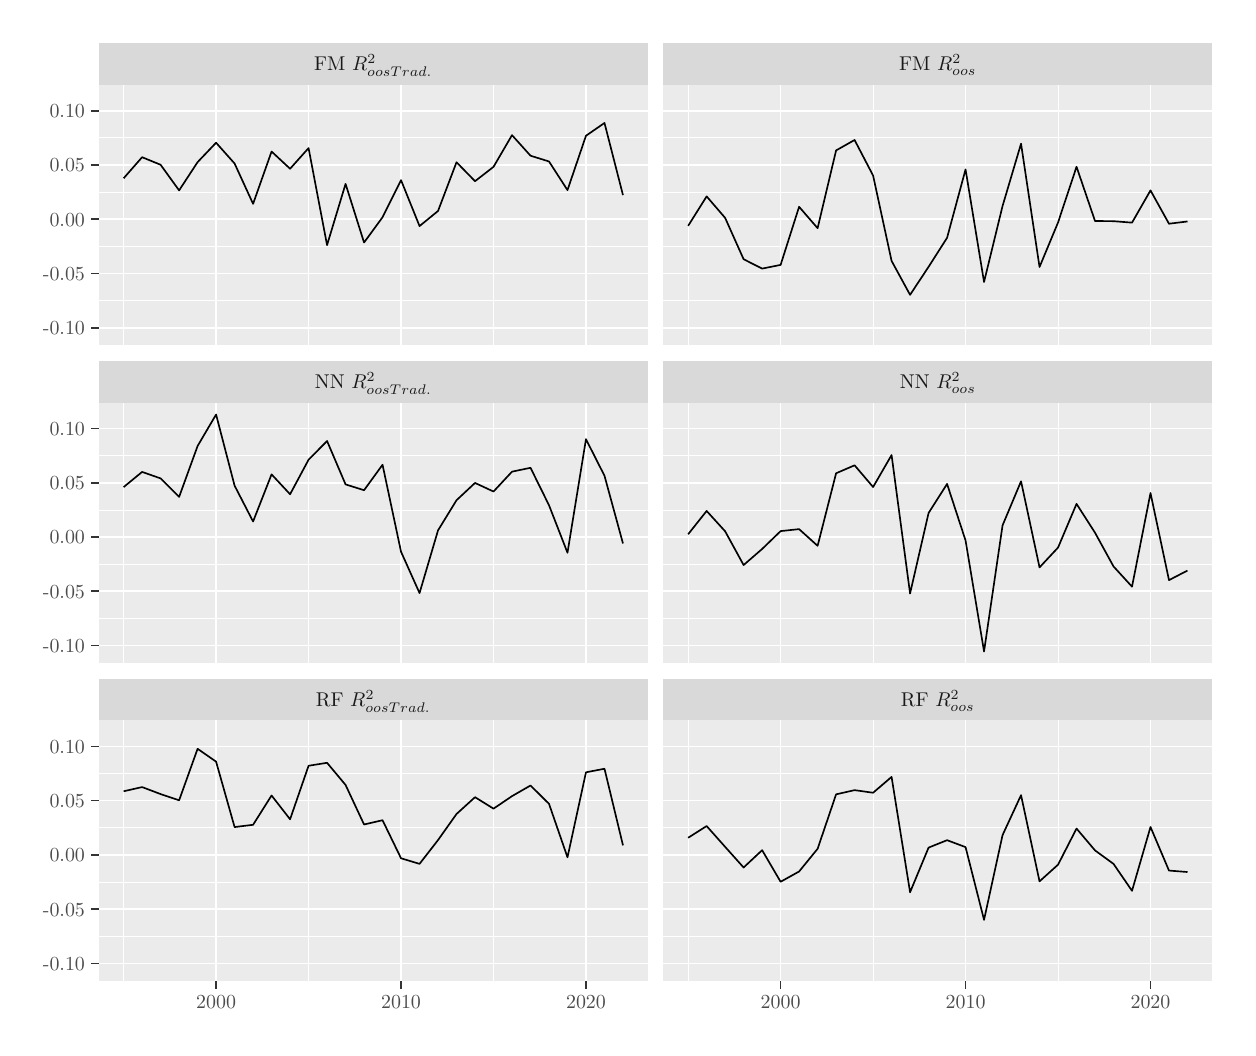
\begin{tikzpicture}[x=1pt,y=1pt]
\definecolor{fillColor}{RGB}{255,255,255}
\path[use as bounding box,fill=fillColor,fill opacity=0.00] (0,0) rectangle (433.62,361.35);
\begin{scope}
\path[clip] (  0.00,  0.00) rectangle (433.62,361.35);
\definecolor{drawColor}{RGB}{255,255,255}
\definecolor{fillColor}{RGB}{255,255,255}

\path[draw=drawColor,line width= 0.6pt,line join=round,line cap=round,fill=fillColor] (  0.00,  0.00) rectangle (433.62,361.35);
\end{scope}
\begin{scope}
\path[clip] ( 25.65,246.50) rectangle (224.13,340.69);
\definecolor{fillColor}{gray}{0.92}

\path[fill=fillColor] ( 25.65,246.50) rectangle (224.13,340.69);
\definecolor{drawColor}{RGB}{255,255,255}

\path[draw=drawColor,line width= 0.3pt,line join=round] ( 25.65,262.73) --
	(224.13,262.73);

\path[draw=drawColor,line width= 0.3pt,line join=round] ( 25.65,282.33) --
	(224.13,282.33);

\path[draw=drawColor,line width= 0.3pt,line join=round] ( 25.65,301.93) --
	(224.13,301.93);

\path[draw=drawColor,line width= 0.3pt,line join=round] ( 25.65,321.53) --
	(224.13,321.53);

\path[draw=drawColor,line width= 0.3pt,line join=round] ( 34.67,246.50) --
	( 34.67,340.69);

\path[draw=drawColor,line width= 0.3pt,line join=round] (101.50,246.50) --
	(101.50,340.69);

\path[draw=drawColor,line width= 0.3pt,line join=round] (168.33,246.50) --
	(168.33,340.69);

\path[draw=drawColor,line width= 0.6pt,line join=round] ( 25.65,252.92) --
	(224.13,252.92);

\path[draw=drawColor,line width= 0.6pt,line join=round] ( 25.65,272.53) --
	(224.13,272.53);

\path[draw=drawColor,line width= 0.6pt,line join=round] ( 25.65,292.13) --
	(224.13,292.13);

\path[draw=drawColor,line width= 0.6pt,line join=round] ( 25.65,311.73) --
	(224.13,311.73);

\path[draw=drawColor,line width= 0.6pt,line join=round] ( 25.65,331.33) --
	(224.13,331.33);

\path[draw=drawColor,line width= 0.6pt,line join=round] ( 68.08,246.50) --
	( 68.08,340.69);

\path[draw=drawColor,line width= 0.6pt,line join=round] (134.91,246.50) --
	(134.91,340.69);

\path[draw=drawColor,line width= 0.6pt,line join=round] (201.74,246.50) --
	(201.74,340.69);
\definecolor{drawColor}{RGB}{0,0,0}

\path[draw=drawColor,line width= 0.6pt,line join=round] ( 34.67,306.92) --
	( 41.35,314.54) --
	( 48.03,311.81) --
	( 54.72,302.55) --
	( 61.40,312.76) --
	( 68.08,319.77) --
	( 74.77,312.26) --
	( 81.45,297.68) --
	( 88.13,316.59) --
	( 94.82,310.37) --
	(101.50,317.84) --
	(108.18,282.78) --
	(114.87,304.90) --
	(121.55,283.71) --
	(128.23,292.84) --
	(134.91,306.26) --
	(141.60,289.65) --
	(148.28,295.11) --
	(154.96,312.72) --
	(161.65,305.87) --
	(168.33,311.06) --
	(175.01,322.51) --
	(181.70,315.08) --
	(188.38,313.00) --
	(195.06,302.65) --
	(201.74,322.29) --
	(208.43,326.91) --
	(215.11,300.85);
\end{scope}
\begin{scope}
\path[clip] ( 25.65,131.66) rectangle (224.13,225.84);
\definecolor{fillColor}{gray}{0.92}

\path[fill=fillColor] ( 25.65,131.66) rectangle (224.13,225.84);
\definecolor{drawColor}{RGB}{255,255,255}

\path[draw=drawColor,line width= 0.3pt,line join=round] ( 25.65,147.88) --
	(224.13,147.88);

\path[draw=drawColor,line width= 0.3pt,line join=round] ( 25.65,167.48) --
	(224.13,167.48);

\path[draw=drawColor,line width= 0.3pt,line join=round] ( 25.65,187.08) --
	(224.13,187.08);

\path[draw=drawColor,line width= 0.3pt,line join=round] ( 25.65,206.68) --
	(224.13,206.68);

\path[draw=drawColor,line width= 0.3pt,line join=round] ( 34.67,131.66) --
	( 34.67,225.84);

\path[draw=drawColor,line width= 0.3pt,line join=round] (101.50,131.66) --
	(101.50,225.84);

\path[draw=drawColor,line width= 0.3pt,line join=round] (168.33,131.66) --
	(168.33,225.84);

\path[draw=drawColor,line width= 0.6pt,line join=round] ( 25.65,138.08) --
	(224.13,138.08);

\path[draw=drawColor,line width= 0.6pt,line join=round] ( 25.65,157.68) --
	(224.13,157.68);

\path[draw=drawColor,line width= 0.6pt,line join=round] ( 25.65,177.28) --
	(224.13,177.28);

\path[draw=drawColor,line width= 0.6pt,line join=round] ( 25.65,196.88) --
	(224.13,196.88);

\path[draw=drawColor,line width= 0.6pt,line join=round] ( 25.65,216.49) --
	(224.13,216.49);

\path[draw=drawColor,line width= 0.6pt,line join=round] ( 68.08,131.66) --
	( 68.08,225.84);

\path[draw=drawColor,line width= 0.6pt,line join=round] (134.91,131.66) --
	(134.91,225.84);

\path[draw=drawColor,line width= 0.6pt,line join=round] (201.74,131.66) --
	(201.74,225.84);
\definecolor{drawColor}{RGB}{0,0,0}

\path[draw=drawColor,line width= 0.6pt,line join=round] ( 34.67,195.33) --
	( 41.35,200.82) --
	( 48.03,198.48) --
	( 54.72,191.78) --
	( 61.40,210.18) --
	( 68.08,221.56) --
	( 74.77,195.85) --
	( 81.45,182.90) --
	( 88.13,199.93) --
	( 94.82,192.75) --
	(101.50,205.22) --
	(108.18,211.99) --
	(114.87,196.31) --
	(121.55,194.21) --
	(128.23,203.41) --
	(134.91,171.98) --
	(141.60,157.04) --
	(148.28,179.70) --
	(154.96,190.59) --
	(161.65,196.84) --
	(168.33,193.73) --
	(175.01,200.91) --
	(181.70,202.31) --
	(188.38,188.78) --
	(195.06,171.61) --
	(201.74,212.64) --
	(208.43,199.43) --
	(215.11,174.97);
\end{scope}
\begin{scope}
\path[clip] ( 25.65, 16.81) rectangle (224.13,111.00);
\definecolor{fillColor}{gray}{0.92}

\path[fill=fillColor] ( 25.65, 16.81) rectangle (224.13,111.00);
\definecolor{drawColor}{RGB}{255,255,255}

\path[draw=drawColor,line width= 0.3pt,line join=round] ( 25.65, 33.03) --
	(224.13, 33.03);

\path[draw=drawColor,line width= 0.3pt,line join=round] ( 25.65, 52.63) --
	(224.13, 52.63);

\path[draw=drawColor,line width= 0.3pt,line join=round] ( 25.65, 72.24) --
	(224.13, 72.24);

\path[draw=drawColor,line width= 0.3pt,line join=round] ( 25.65, 91.84) --
	(224.13, 91.84);

\path[draw=drawColor,line width= 0.3pt,line join=round] ( 34.67, 16.81) --
	( 34.67,111.00);

\path[draw=drawColor,line width= 0.3pt,line join=round] (101.50, 16.81) --
	(101.50,111.00);

\path[draw=drawColor,line width= 0.3pt,line join=round] (168.33, 16.81) --
	(168.33,111.00);

\path[draw=drawColor,line width= 0.6pt,line join=round] ( 25.65, 23.23) --
	(224.13, 23.23);

\path[draw=drawColor,line width= 0.6pt,line join=round] ( 25.65, 42.83) --
	(224.13, 42.83);

\path[draw=drawColor,line width= 0.6pt,line join=round] ( 25.65, 62.43) --
	(224.13, 62.43);

\path[draw=drawColor,line width= 0.6pt,line join=round] ( 25.65, 82.04) --
	(224.13, 82.04);

\path[draw=drawColor,line width= 0.6pt,line join=round] ( 25.65,101.64) --
	(224.13,101.64);

\path[draw=drawColor,line width= 0.6pt,line join=round] ( 68.08, 16.81) --
	( 68.08,111.00);

\path[draw=drawColor,line width= 0.6pt,line join=round] (134.91, 16.81) --
	(134.91,111.00);

\path[draw=drawColor,line width= 0.6pt,line join=round] (201.74, 16.81) --
	(201.74,111.00);
\definecolor{drawColor}{RGB}{0,0,0}

\path[draw=drawColor,line width= 0.6pt,line join=round] ( 34.67, 85.42) --
	( 41.35, 86.94) --
	( 48.03, 84.41) --
	( 54.72, 82.15) --
	( 61.40,100.77) --
	( 68.08, 96.13) --
	( 74.77, 72.49) --
	( 81.45, 73.31) --
	( 88.13, 83.90) --
	( 94.82, 75.30) --
	(101.50, 94.64) --
	(108.18, 95.71) --
	(114.87, 87.71) --
	(121.55, 73.42) --
	(128.23, 74.96) --
	(134.91, 61.21) --
	(141.60, 59.19) --
	(148.28, 67.79) --
	(154.96, 77.21) --
	(161.65, 83.29) --
	(168.33, 79.14) --
	(175.01, 83.66) --
	(181.70, 87.51) --
	(188.38, 80.89) --
	(195.06, 61.56) --
	(201.74, 92.28) --
	(208.43, 93.56) --
	(215.11, 65.89);
\end{scope}
\begin{scope}
\path[clip] (229.63,246.50) rectangle (428.12,340.69);
\definecolor{fillColor}{gray}{0.92}

\path[fill=fillColor] (229.63,246.50) rectangle (428.12,340.69);
\definecolor{drawColor}{RGB}{255,255,255}

\path[draw=drawColor,line width= 0.3pt,line join=round] (229.63,262.73) --
	(428.12,262.73);

\path[draw=drawColor,line width= 0.3pt,line join=round] (229.63,282.33) --
	(428.12,282.33);

\path[draw=drawColor,line width= 0.3pt,line join=round] (229.63,301.93) --
	(428.12,301.93);

\path[draw=drawColor,line width= 0.3pt,line join=round] (229.63,321.53) --
	(428.12,321.53);

\path[draw=drawColor,line width= 0.3pt,line join=round] (238.66,246.50) --
	(238.66,340.69);

\path[draw=drawColor,line width= 0.3pt,line join=round] (305.49,246.50) --
	(305.49,340.69);

\path[draw=drawColor,line width= 0.3pt,line join=round] (372.32,246.50) --
	(372.32,340.69);

\path[draw=drawColor,line width= 0.6pt,line join=round] (229.63,252.92) --
	(428.12,252.92);

\path[draw=drawColor,line width= 0.6pt,line join=round] (229.63,272.53) --
	(428.12,272.53);

\path[draw=drawColor,line width= 0.6pt,line join=round] (229.63,292.13) --
	(428.12,292.13);

\path[draw=drawColor,line width= 0.6pt,line join=round] (229.63,311.73) --
	(428.12,311.73);

\path[draw=drawColor,line width= 0.6pt,line join=round] (229.63,331.33) --
	(428.12,331.33);

\path[draw=drawColor,line width= 0.6pt,line join=round] (272.07,246.50) --
	(272.07,340.69);

\path[draw=drawColor,line width= 0.6pt,line join=round] (338.90,246.50) --
	(338.90,340.69);

\path[draw=drawColor,line width= 0.6pt,line join=round] (405.73,246.50) --
	(405.73,340.69);
\definecolor{drawColor}{RGB}{0,0,0}

\path[draw=drawColor,line width= 0.6pt,line join=round] (238.66,289.74) --
	(245.34,300.38) --
	(252.02,292.62) --
	(258.70,277.68) --
	(265.39,274.28) --
	(272.07,275.62) --
	(278.75,296.62) --
	(285.44,288.89) --
	(292.12,316.99) --
	(298.80,320.76) --
	(305.49,307.91) --
	(312.17,277.07) --
	(318.85,264.81) --
	(325.54,274.93) --
	(332.22,285.41) --
	(338.90,310.13) --
	(345.58,269.46) --
	(352.27,296.91) --
	(358.95,319.42) --
	(365.63,274.87) --
	(372.32,290.94) --
	(379.00,311.09) --
	(385.68,291.49) --
	(392.37,291.42) --
	(399.05,290.89) --
	(405.73,302.54) --
	(412.41,290.50) --
	(419.10,291.32);
\end{scope}
\begin{scope}
\path[clip] (229.63,131.66) rectangle (428.12,225.84);
\definecolor{fillColor}{gray}{0.92}

\path[fill=fillColor] (229.63,131.66) rectangle (428.12,225.84);
\definecolor{drawColor}{RGB}{255,255,255}

\path[draw=drawColor,line width= 0.3pt,line join=round] (229.63,147.88) --
	(428.12,147.88);

\path[draw=drawColor,line width= 0.3pt,line join=round] (229.63,167.48) --
	(428.12,167.48);

\path[draw=drawColor,line width= 0.3pt,line join=round] (229.63,187.08) --
	(428.12,187.08);

\path[draw=drawColor,line width= 0.3pt,line join=round] (229.63,206.68) --
	(428.12,206.68);

\path[draw=drawColor,line width= 0.3pt,line join=round] (238.66,131.66) --
	(238.66,225.84);

\path[draw=drawColor,line width= 0.3pt,line join=round] (305.49,131.66) --
	(305.49,225.84);

\path[draw=drawColor,line width= 0.3pt,line join=round] (372.32,131.66) --
	(372.32,225.84);

\path[draw=drawColor,line width= 0.6pt,line join=round] (229.63,138.08) --
	(428.12,138.08);

\path[draw=drawColor,line width= 0.6pt,line join=round] (229.63,157.68) --
	(428.12,157.68);

\path[draw=drawColor,line width= 0.6pt,line join=round] (229.63,177.28) --
	(428.12,177.28);

\path[draw=drawColor,line width= 0.6pt,line join=round] (229.63,196.88) --
	(428.12,196.88);

\path[draw=drawColor,line width= 0.6pt,line join=round] (229.63,216.49) --
	(428.12,216.49);

\path[draw=drawColor,line width= 0.6pt,line join=round] (272.07,131.66) --
	(272.07,225.84);

\path[draw=drawColor,line width= 0.6pt,line join=round] (338.90,131.66) --
	(338.90,225.84);

\path[draw=drawColor,line width= 0.6pt,line join=round] (405.73,131.66) --
	(405.73,225.84);
\definecolor{drawColor}{RGB}{0,0,0}

\path[draw=drawColor,line width= 0.6pt,line join=round] (238.66,178.30) --
	(245.34,186.71) --
	(252.02,179.37) --
	(258.70,167.17) --
	(265.39,172.97) --
	(272.07,179.43) --
	(278.75,180.15) --
	(285.44,174.11) --
	(292.12,200.33) --
	(298.80,203.21) --
	(305.49,195.36) --
	(312.17,206.91) --
	(318.85,156.89) --
	(325.54,185.98) --
	(332.22,196.47) --
	(338.90,176.05) --
	(345.58,135.94) --
	(352.27,181.50) --
	(358.95,197.43) --
	(365.63,166.32) --
	(372.32,173.48) --
	(379.00,189.27) --
	(385.68,178.85) --
	(392.37,166.66) --
	(399.05,159.35) --
	(405.73,193.18) --
	(412.41,161.72) --
	(419.10,165.18);
\end{scope}
\begin{scope}
\path[clip] (229.63, 16.81) rectangle (428.12,111.00);
\definecolor{fillColor}{gray}{0.92}

\path[fill=fillColor] (229.63, 16.81) rectangle (428.12,111.00);
\definecolor{drawColor}{RGB}{255,255,255}

\path[draw=drawColor,line width= 0.3pt,line join=round] (229.63, 33.03) --
	(428.12, 33.03);

\path[draw=drawColor,line width= 0.3pt,line join=round] (229.63, 52.63) --
	(428.12, 52.63);

\path[draw=drawColor,line width= 0.3pt,line join=round] (229.63, 72.24) --
	(428.12, 72.24);

\path[draw=drawColor,line width= 0.3pt,line join=round] (229.63, 91.84) --
	(428.12, 91.84);

\path[draw=drawColor,line width= 0.3pt,line join=round] (238.66, 16.81) --
	(238.66,111.00);

\path[draw=drawColor,line width= 0.3pt,line join=round] (305.49, 16.81) --
	(305.49,111.00);

\path[draw=drawColor,line width= 0.3pt,line join=round] (372.32, 16.81) --
	(372.32,111.00);

\path[draw=drawColor,line width= 0.6pt,line join=round] (229.63, 23.23) --
	(428.12, 23.23);

\path[draw=drawColor,line width= 0.6pt,line join=round] (229.63, 42.83) --
	(428.12, 42.83);

\path[draw=drawColor,line width= 0.6pt,line join=round] (229.63, 62.43) --
	(428.12, 62.43);

\path[draw=drawColor,line width= 0.6pt,line join=round] (229.63, 82.04) --
	(428.12, 82.04);

\path[draw=drawColor,line width= 0.6pt,line join=round] (229.63,101.64) --
	(428.12,101.64);

\path[draw=drawColor,line width= 0.6pt,line join=round] (272.07, 16.81) --
	(272.07,111.00);

\path[draw=drawColor,line width= 0.6pt,line join=round] (338.90, 16.81) --
	(338.90,111.00);

\path[draw=drawColor,line width= 0.6pt,line join=round] (405.73, 16.81) --
	(405.73,111.00);
\definecolor{drawColor}{RGB}{0,0,0}

\path[draw=drawColor,line width= 0.6pt,line join=round] (238.66, 68.62) --
	(245.34, 72.86) --
	(252.02, 65.34) --
	(258.70, 57.88) --
	(265.39, 64.13) --
	(272.07, 52.72) --
	(278.75, 56.43) --
	(285.44, 64.64) --
	(292.12, 84.31) --
	(298.80, 85.83) --
	(305.49, 84.89) --
	(312.17, 90.61) --
	(318.85, 48.94) --
	(325.54, 65.06) --
	(332.22, 67.75) --
	(338.90, 65.24) --
	(345.58, 38.96) --
	(352.27, 69.58) --
	(358.95, 84.01) --
	(365.63, 52.87) --
	(372.32, 58.90) --
	(379.00, 71.95) --
	(385.68, 64.06) --
	(392.37, 59.18) --
	(399.05, 49.45) --
	(405.73, 72.52) --
	(412.41, 56.77) --
	(419.10, 56.24);
\end{scope}
\begin{scope}
\path[clip] ( 25.65,111.00) rectangle (224.13,126.16);
\definecolor{fillColor}{gray}{0.85}

\path[fill=fillColor] ( 25.65,111.00) rectangle (224.13,126.16);
\definecolor{drawColor}{gray}{0.10}

\node[text=drawColor,anchor=base,inner sep=0pt, outer sep=0pt, scale=  0.72] at (124.89,116.10) {RF $R^2_{oos  Trad.}$};
\end{scope}
\begin{scope}
\path[clip] (229.63,111.00) rectangle (428.12,126.16);
\definecolor{fillColor}{gray}{0.85}

\path[fill=fillColor] (229.63,111.00) rectangle (428.12,126.16);
\definecolor{drawColor}{gray}{0.10}

\node[text=drawColor,anchor=base,inner sep=0pt, outer sep=0pt, scale=  0.72] at (328.88,116.10) {RF $R^2_{oos}$};
\end{scope}
\begin{scope}
\path[clip] ( 25.65,225.84) rectangle (224.13,241.00);
\definecolor{fillColor}{gray}{0.85}

\path[fill=fillColor] ( 25.65,225.84) rectangle (224.13,241.00);
\definecolor{drawColor}{gray}{0.10}

\node[text=drawColor,anchor=base,inner sep=0pt, outer sep=0pt, scale=  0.72] at (124.89,230.94) {NN $R^2_{oos  Trad.}$};
\end{scope}
\begin{scope}
\path[clip] (229.63,225.84) rectangle (428.12,241.00);
\definecolor{fillColor}{gray}{0.85}

\path[fill=fillColor] (229.63,225.84) rectangle (428.12,241.00);
\definecolor{drawColor}{gray}{0.10}

\node[text=drawColor,anchor=base,inner sep=0pt, outer sep=0pt, scale=  0.72] at (328.88,230.94) {NN $R^2_{oos}$};
\end{scope}
\begin{scope}
\path[clip] ( 25.65,340.69) rectangle (224.13,355.85);
\definecolor{fillColor}{gray}{0.85}

\path[fill=fillColor] ( 25.65,340.69) rectangle (224.13,355.85);
\definecolor{drawColor}{gray}{0.10}

\node[text=drawColor,anchor=base,inner sep=0pt, outer sep=0pt, scale=  0.72] at (124.89,345.79) {FM $R^2_{oos  Trad.}$};
\end{scope}
\begin{scope}
\path[clip] (229.63,340.69) rectangle (428.12,355.85);
\definecolor{fillColor}{gray}{0.85}

\path[fill=fillColor] (229.63,340.69) rectangle (428.12,355.85);
\definecolor{drawColor}{gray}{0.10}

\node[text=drawColor,anchor=base,inner sep=0pt, outer sep=0pt, scale=  0.72] at (328.88,345.79) {FM $R^2_{oos}$};
\end{scope}
\begin{scope}
\path[clip] (  0.00,  0.00) rectangle (433.62,361.35);
\definecolor{drawColor}{gray}{0.20}

\path[draw=drawColor,line width= 0.6pt,line join=round] ( 68.08, 14.06) --
	( 68.08, 16.81);

\path[draw=drawColor,line width= 0.6pt,line join=round] (134.91, 14.06) --
	(134.91, 16.81);

\path[draw=drawColor,line width= 0.6pt,line join=round] (201.74, 14.06) --
	(201.74, 16.81);
\end{scope}
\begin{scope}
\path[clip] (  0.00,  0.00) rectangle (433.62,361.35);
\definecolor{drawColor}{gray}{0.30}

\node[text=drawColor,anchor=base,inner sep=0pt, outer sep=0pt, scale=  0.72] at ( 68.08,  6.90) {2000};

\node[text=drawColor,anchor=base,inner sep=0pt, outer sep=0pt, scale=  0.72] at (134.91,  6.90) {2010};

\node[text=drawColor,anchor=base,inner sep=0pt, outer sep=0pt, scale=  0.72] at (201.74,  6.90) {2020};
\end{scope}
\begin{scope}
\path[clip] (  0.00,  0.00) rectangle (433.62,361.35);
\definecolor{drawColor}{gray}{0.20}

\path[draw=drawColor,line width= 0.6pt,line join=round] (272.07, 14.06) --
	(272.07, 16.81);

\path[draw=drawColor,line width= 0.6pt,line join=round] (338.90, 14.06) --
	(338.90, 16.81);

\path[draw=drawColor,line width= 0.6pt,line join=round] (405.73, 14.06) --
	(405.73, 16.81);
\end{scope}
\begin{scope}
\path[clip] (  0.00,  0.00) rectangle (433.62,361.35);
\definecolor{drawColor}{gray}{0.30}

\node[text=drawColor,anchor=base,inner sep=0pt, outer sep=0pt, scale=  0.72] at (272.07,  6.90) {2000};

\node[text=drawColor,anchor=base,inner sep=0pt, outer sep=0pt, scale=  0.72] at (338.90,  6.90) {2010};

\node[text=drawColor,anchor=base,inner sep=0pt, outer sep=0pt, scale=  0.72] at (405.73,  6.90) {2020};
\end{scope}
\begin{scope}
\path[clip] (  0.00,  0.00) rectangle (433.62,361.35);
\definecolor{drawColor}{gray}{0.30}

\node[text=drawColor,anchor=base east,inner sep=0pt, outer sep=0pt, scale=  0.72] at ( 20.70,250.44) {-0.10};

\node[text=drawColor,anchor=base east,inner sep=0pt, outer sep=0pt, scale=  0.72] at ( 20.70,270.05) {-0.05};

\node[text=drawColor,anchor=base east,inner sep=0pt, outer sep=0pt, scale=  0.72] at ( 20.70,289.65) {0.00};

\node[text=drawColor,anchor=base east,inner sep=0pt, outer sep=0pt, scale=  0.72] at ( 20.70,309.25) {0.05};

\node[text=drawColor,anchor=base east,inner sep=0pt, outer sep=0pt, scale=  0.72] at ( 20.70,328.85) {0.10};
\end{scope}
\begin{scope}
\path[clip] (  0.00,  0.00) rectangle (433.62,361.35);
\definecolor{drawColor}{gray}{0.20}

\path[draw=drawColor,line width= 0.6pt,line join=round] ( 22.90,252.92) --
	( 25.65,252.92);

\path[draw=drawColor,line width= 0.6pt,line join=round] ( 22.90,272.53) --
	( 25.65,272.53);

\path[draw=drawColor,line width= 0.6pt,line join=round] ( 22.90,292.13) --
	( 25.65,292.13);

\path[draw=drawColor,line width= 0.6pt,line join=round] ( 22.90,311.73) --
	( 25.65,311.73);

\path[draw=drawColor,line width= 0.6pt,line join=round] ( 22.90,331.33) --
	( 25.65,331.33);
\end{scope}
\begin{scope}
\path[clip] (  0.00,  0.00) rectangle (433.62,361.35);
\definecolor{drawColor}{gray}{0.30}

\node[text=drawColor,anchor=base east,inner sep=0pt, outer sep=0pt, scale=  0.72] at ( 20.70,135.60) {-0.10};

\node[text=drawColor,anchor=base east,inner sep=0pt, outer sep=0pt, scale=  0.72] at ( 20.70,155.20) {-0.05};

\node[text=drawColor,anchor=base east,inner sep=0pt, outer sep=0pt, scale=  0.72] at ( 20.70,174.80) {0.00};

\node[text=drawColor,anchor=base east,inner sep=0pt, outer sep=0pt, scale=  0.72] at ( 20.70,194.40) {0.05};

\node[text=drawColor,anchor=base east,inner sep=0pt, outer sep=0pt, scale=  0.72] at ( 20.70,214.01) {0.10};
\end{scope}
\begin{scope}
\path[clip] (  0.00,  0.00) rectangle (433.62,361.35);
\definecolor{drawColor}{gray}{0.20}

\path[draw=drawColor,line width= 0.6pt,line join=round] ( 22.90,138.08) --
	( 25.65,138.08);

\path[draw=drawColor,line width= 0.6pt,line join=round] ( 22.90,157.68) --
	( 25.65,157.68);

\path[draw=drawColor,line width= 0.6pt,line join=round] ( 22.90,177.28) --
	( 25.65,177.28);

\path[draw=drawColor,line width= 0.6pt,line join=round] ( 22.90,196.88) --
	( 25.65,196.88);

\path[draw=drawColor,line width= 0.6pt,line join=round] ( 22.90,216.49) --
	( 25.65,216.49);
\end{scope}
\begin{scope}
\path[clip] (  0.00,  0.00) rectangle (433.62,361.35);
\definecolor{drawColor}{gray}{0.30}

\node[text=drawColor,anchor=base east,inner sep=0pt, outer sep=0pt, scale=  0.72] at ( 20.70, 20.75) {-0.10};

\node[text=drawColor,anchor=base east,inner sep=0pt, outer sep=0pt, scale=  0.72] at ( 20.70, 40.35) {-0.05};

\node[text=drawColor,anchor=base east,inner sep=0pt, outer sep=0pt, scale=  0.72] at ( 20.70, 59.95) {0.00};

\node[text=drawColor,anchor=base east,inner sep=0pt, outer sep=0pt, scale=  0.72] at ( 20.70, 79.56) {0.05};

\node[text=drawColor,anchor=base east,inner sep=0pt, outer sep=0pt, scale=  0.72] at ( 20.70, 99.16) {0.10};
\end{scope}
\begin{scope}
\path[clip] (  0.00,  0.00) rectangle (433.62,361.35);
\definecolor{drawColor}{gray}{0.20}

\path[draw=drawColor,line width= 0.6pt,line join=round] ( 22.90, 23.23) --
	( 25.65, 23.23);

\path[draw=drawColor,line width= 0.6pt,line join=round] ( 22.90, 42.83) --
	( 25.65, 42.83);

\path[draw=drawColor,line width= 0.6pt,line join=round] ( 22.90, 62.43) --
	( 25.65, 62.43);

\path[draw=drawColor,line width= 0.6pt,line join=round] ( 22.90, 82.04) --
	( 25.65, 82.04);

\path[draw=drawColor,line width= 0.6pt,line join=round] ( 22.90,101.64) --
	( 25.65,101.64);
\end{scope}
\end{tikzpicture}

\label{plot:OOSR2_ts}
\end{figure}

\begin{figure}[ht]
\centering
\caption[Turnover of highest epected return portfolios]{\textbf{Turnover of highest epected return portfolios}\\ .}
% Created by tikzDevice version 0.12.6 on 2024-03-11 18:45:03
% !TEX encoding = UTF-8 Unicode
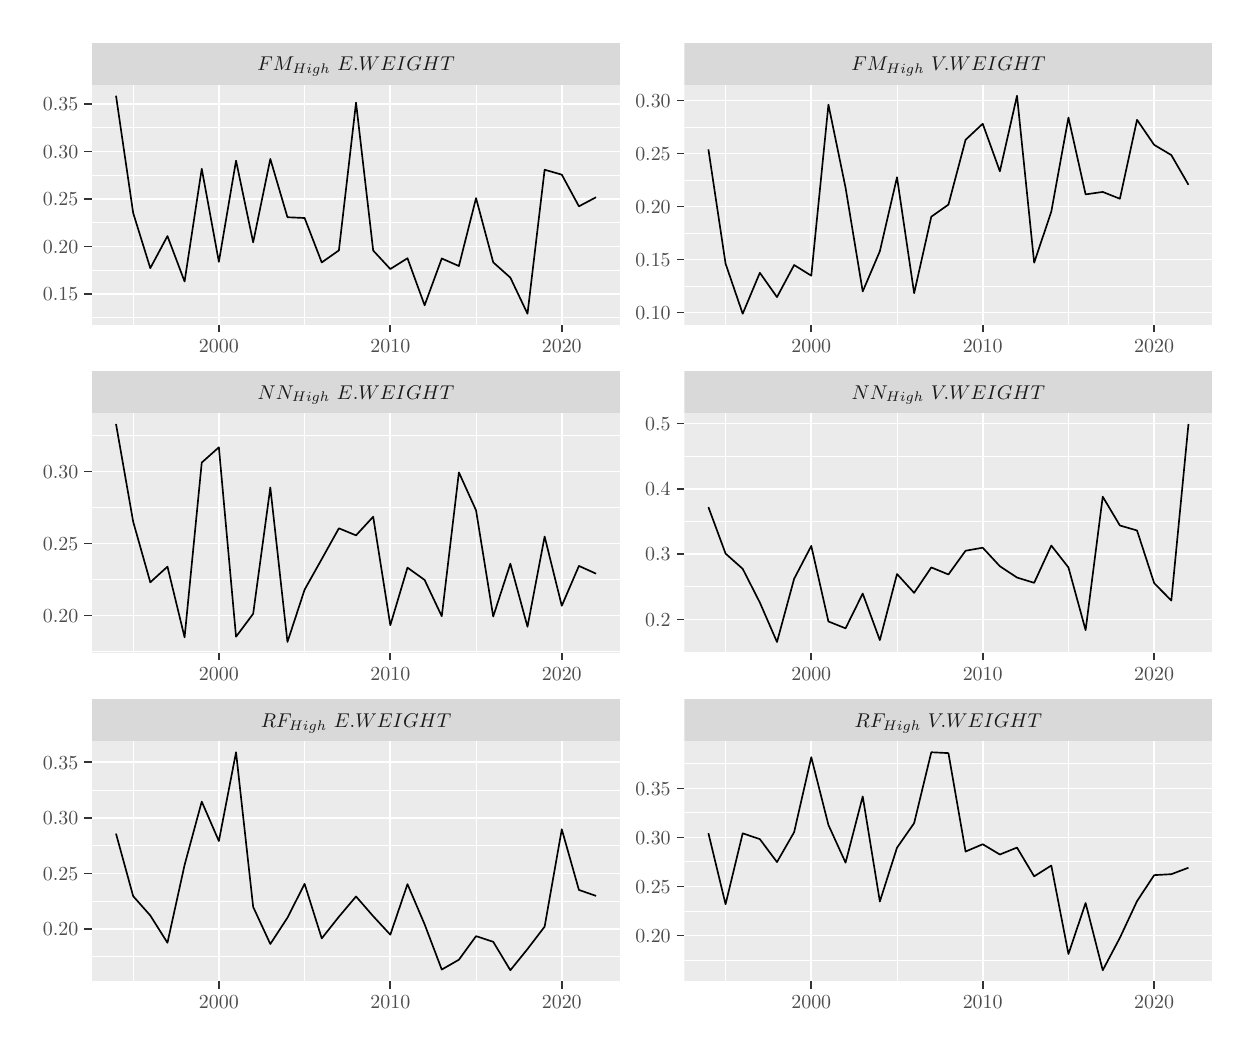
\begin{tikzpicture}[x=1pt,y=1pt]
\definecolor{fillColor}{RGB}{255,255,255}
\path[use as bounding box,fill=fillColor,fill opacity=0.00] (0,0) rectangle (433.62,361.35);
\begin{scope}
\path[clip] (  0.00,  0.00) rectangle (433.62,361.35);
\definecolor{drawColor}{RGB}{255,255,255}
\definecolor{fillColor}{RGB}{255,255,255}

\path[draw=drawColor,line width= 0.6pt,line join=round,line cap=round,fill=fillColor] (  0.00,  0.00) rectangle (433.62,361.35);
\end{scope}
\begin{scope}
\path[clip] ( 23.25,254.04) rectangle (214.06,340.69);
\definecolor{fillColor}{gray}{0.92}

\path[fill=fillColor] ( 23.25,254.04) rectangle (214.06,340.69);
\definecolor{drawColor}{RGB}{255,255,255}

\path[draw=drawColor,line width= 0.3pt,line join=round] ( 23.25,256.50) --
	(214.06,256.50);

\path[draw=drawColor,line width= 0.3pt,line join=round] ( 23.25,273.67) --
	(214.06,273.67);

\path[draw=drawColor,line width= 0.3pt,line join=round] ( 23.25,290.84) --
	(214.06,290.84);

\path[draw=drawColor,line width= 0.3pt,line join=round] ( 23.25,308.01) --
	(214.06,308.01);

\path[draw=drawColor,line width= 0.3pt,line join=round] ( 23.25,325.18) --
	(214.06,325.18);

\path[draw=drawColor,line width= 0.3pt,line join=round] ( 38.12,254.04) --
	( 38.12,340.69);

\path[draw=drawColor,line width= 0.3pt,line join=round] (100.07,254.04) --
	(100.07,340.69);

\path[draw=drawColor,line width= 0.3pt,line join=round] (162.02,254.04) --
	(162.02,340.69);

\path[draw=drawColor,line width= 0.6pt,line join=round] ( 23.25,265.09) --
	(214.06,265.09);

\path[draw=drawColor,line width= 0.6pt,line join=round] ( 23.25,282.26) --
	(214.06,282.26);

\path[draw=drawColor,line width= 0.6pt,line join=round] ( 23.25,299.43) --
	(214.06,299.43);

\path[draw=drawColor,line width= 0.6pt,line join=round] ( 23.25,316.60) --
	(214.06,316.60);

\path[draw=drawColor,line width= 0.6pt,line join=round] ( 23.25,333.77) --
	(214.06,333.77);

\path[draw=drawColor,line width= 0.6pt,line join=round] ( 69.09,254.04) --
	( 69.09,340.69);

\path[draw=drawColor,line width= 0.6pt,line join=round] (131.04,254.04) --
	(131.04,340.69);

\path[draw=drawColor,line width= 0.6pt,line join=round] (193.00,254.04) --
	(193.00,340.69);
\definecolor{drawColor}{RGB}{0,0,0}

\path[draw=drawColor,line width= 0.6pt,line join=round] ( 31.92,336.75) --
	( 38.12,294.39) --
	( 44.31,274.45) --
	( 50.51,286.04) --
	( 56.70,269.63) --
	( 62.90,310.37) --
	( 69.09,276.73) --
	( 75.29,313.29) --
	( 81.48,283.78) --
	( 87.68,313.91) --
	( 93.87,292.85) --
	(100.07,292.57) --
	(106.26,276.51) --
	(112.46,280.87) --
	(118.65,334.26) --
	(124.85,280.82) --
	(131.04,274.13) --
	(137.24,278.03) --
	(143.43,261.03) --
	(149.63,277.94) --
	(155.82,275.22) --
	(162.02,299.75) --
	(168.22,276.55) --
	(174.41,271.03) --
	(180.61,257.98) --
	(186.80,310.01) --
	(193.00,308.24) --
	(199.19,296.79) --
	(205.39,300.07);
\end{scope}
\begin{scope}
\path[clip] ( 23.25,135.43) rectangle (214.06,222.07);
\definecolor{fillColor}{gray}{0.92}

\path[fill=fillColor] ( 23.25,135.43) rectangle (214.06,222.07);
\definecolor{drawColor}{RGB}{255,255,255}

\path[draw=drawColor,line width= 0.3pt,line join=round] ( 23.25,135.94) --
	(214.06,135.94);

\path[draw=drawColor,line width= 0.3pt,line join=round] ( 23.25,161.96) --
	(214.06,161.96);

\path[draw=drawColor,line width= 0.3pt,line join=round] ( 23.25,187.98) --
	(214.06,187.98);

\path[draw=drawColor,line width= 0.3pt,line join=round] ( 23.25,214.00) --
	(214.06,214.00);

\path[draw=drawColor,line width= 0.3pt,line join=round] ( 38.12,135.43) --
	( 38.12,222.07);

\path[draw=drawColor,line width= 0.3pt,line join=round] (100.07,135.43) --
	(100.07,222.07);

\path[draw=drawColor,line width= 0.3pt,line join=round] (162.02,135.43) --
	(162.02,222.07);

\path[draw=drawColor,line width= 0.6pt,line join=round] ( 23.25,148.95) --
	(214.06,148.95);

\path[draw=drawColor,line width= 0.6pt,line join=round] ( 23.25,174.97) --
	(214.06,174.97);

\path[draw=drawColor,line width= 0.6pt,line join=round] ( 23.25,200.99) --
	(214.06,200.99);

\path[draw=drawColor,line width= 0.6pt,line join=round] ( 69.09,135.43) --
	( 69.09,222.07);

\path[draw=drawColor,line width= 0.6pt,line join=round] (131.04,135.43) --
	(131.04,222.07);

\path[draw=drawColor,line width= 0.6pt,line join=round] (193.00,135.43) --
	(193.00,222.07);
\definecolor{drawColor}{RGB}{0,0,0}

\path[draw=drawColor,line width= 0.6pt,line join=round] ( 31.92,218.14) --
	( 38.12,182.84) --
	( 44.31,160.94) --
	( 50.51,166.59) --
	( 56.70,141.06) --
	( 62.90,204.19) --
	( 69.09,209.72) --
	( 75.29,141.28) --
	( 81.48,149.55) --
	( 87.68,195.19) --
	( 93.87,139.36) --
	(100.07,158.28) --
	(106.26,169.32) --
	(112.46,180.45) --
	(118.65,177.89) --
	(124.85,184.63) --
	(131.04,145.43) --
	(137.24,166.23) --
	(143.43,161.79) --
	(149.63,148.67) --
	(155.82,200.65) --
	(162.02,186.92) --
	(168.22,148.57) --
	(174.41,167.65) --
	(180.61,144.88) --
	(186.80,177.47) --
	(193.00,152.44) --
	(199.19,166.85) --
	(205.39,164.05);
\end{scope}
\begin{scope}
\path[clip] ( 23.25, 16.81) rectangle (214.06,103.46);
\definecolor{fillColor}{gray}{0.92}

\path[fill=fillColor] ( 23.25, 16.81) rectangle (214.06,103.46);
\definecolor{drawColor}{RGB}{255,255,255}

\path[draw=drawColor,line width= 0.3pt,line join=round] ( 23.25, 25.58) --
	(214.06, 25.58);

\path[draw=drawColor,line width= 0.3pt,line join=round] ( 23.25, 45.68) --
	(214.06, 45.68);

\path[draw=drawColor,line width= 0.3pt,line join=round] ( 23.25, 65.79) --
	(214.06, 65.79);

\path[draw=drawColor,line width= 0.3pt,line join=round] ( 23.25, 85.89) --
	(214.06, 85.89);

\path[draw=drawColor,line width= 0.3pt,line join=round] ( 38.12, 16.81) --
	( 38.12,103.46);

\path[draw=drawColor,line width= 0.3pt,line join=round] (100.07, 16.81) --
	(100.07,103.46);

\path[draw=drawColor,line width= 0.3pt,line join=round] (162.02, 16.81) --
	(162.02,103.46);

\path[draw=drawColor,line width= 0.6pt,line join=round] ( 23.25, 35.63) --
	(214.06, 35.63);

\path[draw=drawColor,line width= 0.6pt,line join=round] ( 23.25, 55.74) --
	(214.06, 55.74);

\path[draw=drawColor,line width= 0.6pt,line join=round] ( 23.25, 75.84) --
	(214.06, 75.84);

\path[draw=drawColor,line width= 0.6pt,line join=round] ( 23.25, 95.95) --
	(214.06, 95.95);

\path[draw=drawColor,line width= 0.6pt,line join=round] ( 69.09, 16.81) --
	( 69.09,103.46);

\path[draw=drawColor,line width= 0.6pt,line join=round] (131.04, 16.81) --
	(131.04,103.46);

\path[draw=drawColor,line width= 0.6pt,line join=round] (193.00, 16.81) --
	(193.00,103.46);
\definecolor{drawColor}{RGB}{0,0,0}

\path[draw=drawColor,line width= 0.6pt,line join=round] ( 31.92, 70.11) --
	( 38.12, 47.52) --
	( 44.31, 40.53) --
	( 50.51, 30.68) --
	( 56.70, 58.79) --
	( 62.90, 81.69) --
	( 69.09, 67.43) --
	( 75.29, 99.52) --
	( 81.48, 43.63) --
	( 87.68, 30.23) --
	( 93.87, 39.73) --
	(100.07, 51.96) --
	(106.26, 32.26) --
	(112.46, 40.08) --
	(118.65, 47.41) --
	(124.85, 40.28) --
	(131.04, 33.60) --
	(137.24, 51.86) --
	(143.43, 37.36) --
	(149.63, 21.00) --
	(155.82, 24.55) --
	(162.02, 33.07) --
	(168.22, 31.04) --
	(174.41, 20.75) --
	(180.61, 28.41) --
	(186.80, 36.51) --
	(193.00, 71.68) --
	(199.19, 49.78) --
	(205.39, 47.61);
\end{scope}
\begin{scope}
\path[clip] (237.31,254.04) rectangle (428.12,340.69);
\definecolor{fillColor}{gray}{0.92}

\path[fill=fillColor] (237.31,254.04) rectangle (428.12,340.69);
\definecolor{drawColor}{RGB}{255,255,255}

\path[draw=drawColor,line width= 0.3pt,line join=round] (237.31,267.96) --
	(428.12,267.96);

\path[draw=drawColor,line width= 0.3pt,line join=round] (237.31,287.11) --
	(428.12,287.11);

\path[draw=drawColor,line width= 0.3pt,line join=round] (237.31,306.27) --
	(428.12,306.27);

\path[draw=drawColor,line width= 0.3pt,line join=round] (237.31,325.43) --
	(428.12,325.43);

\path[draw=drawColor,line width= 0.3pt,line join=round] (252.18,254.04) --
	(252.18,340.69);

\path[draw=drawColor,line width= 0.3pt,line join=round] (314.13,254.04) --
	(314.13,340.69);

\path[draw=drawColor,line width= 0.3pt,line join=round] (376.08,254.04) --
	(376.08,340.69);

\path[draw=drawColor,line width= 0.6pt,line join=round] (237.31,258.38) --
	(428.12,258.38);

\path[draw=drawColor,line width= 0.6pt,line join=round] (237.31,277.53) --
	(428.12,277.53);

\path[draw=drawColor,line width= 0.6pt,line join=round] (237.31,296.69) --
	(428.12,296.69);

\path[draw=drawColor,line width= 0.6pt,line join=round] (237.31,315.85) --
	(428.12,315.85);

\path[draw=drawColor,line width= 0.6pt,line join=round] (237.31,335.01) --
	(428.12,335.01);

\path[draw=drawColor,line width= 0.6pt,line join=round] (283.15,254.04) --
	(283.15,340.69);

\path[draw=drawColor,line width= 0.6pt,line join=round] (345.10,254.04) --
	(345.10,340.69);

\path[draw=drawColor,line width= 0.6pt,line join=round] (407.06,254.04) --
	(407.06,340.69);
\definecolor{drawColor}{RGB}{0,0,0}

\path[draw=drawColor,line width= 0.6pt,line join=round] (245.98,317.36) --
	(252.18,276.08) --
	(258.37,257.98) --
	(264.57,272.78) --
	(270.76,263.99) --
	(276.96,275.58) --
	(283.15,271.73) --
	(289.35,333.54) --
	(295.54,303.51) --
	(301.74,266.03) --
	(307.93,280.56) --
	(314.13,307.29) --
	(320.32,265.40) --
	(326.52,293.04) --
	(332.71,297.41) --
	(338.91,320.83) --
	(345.10,326.62) --
	(351.30,309.44) --
	(357.49,336.75) --
	(363.69,276.42) --
	(369.88,294.86) --
	(376.08,328.86) --
	(382.28,301.11) --
	(388.47,301.99) --
	(394.67,299.53) --
	(400.86,328.05) --
	(407.06,318.99) --
	(413.25,315.31) --
	(419.45,304.57);
\end{scope}
\begin{scope}
\path[clip] (237.31,135.43) rectangle (428.12,222.07);
\definecolor{fillColor}{gray}{0.92}

\path[fill=fillColor] (237.31,135.43) rectangle (428.12,222.07);
\definecolor{drawColor}{RGB}{255,255,255}

\path[draw=drawColor,line width= 0.3pt,line join=round] (237.31,135.76) --
	(428.12,135.76);

\path[draw=drawColor,line width= 0.3pt,line join=round] (237.31,159.34) --
	(428.12,159.34);

\path[draw=drawColor,line width= 0.3pt,line join=round] (237.31,182.91) --
	(428.12,182.91);

\path[draw=drawColor,line width= 0.3pt,line join=round] (237.31,206.49) --
	(428.12,206.49);

\path[draw=drawColor,line width= 0.3pt,line join=round] (252.18,135.43) --
	(252.18,222.07);

\path[draw=drawColor,line width= 0.3pt,line join=round] (314.13,135.43) --
	(314.13,222.07);

\path[draw=drawColor,line width= 0.3pt,line join=round] (376.08,135.43) --
	(376.08,222.07);

\path[draw=drawColor,line width= 0.6pt,line join=round] (237.31,147.55) --
	(428.12,147.55);

\path[draw=drawColor,line width= 0.6pt,line join=round] (237.31,171.12) --
	(428.12,171.12);

\path[draw=drawColor,line width= 0.6pt,line join=round] (237.31,194.70) --
	(428.12,194.70);

\path[draw=drawColor,line width= 0.6pt,line join=round] (237.31,218.28) --
	(428.12,218.28);

\path[draw=drawColor,line width= 0.6pt,line join=round] (283.15,135.43) --
	(283.15,222.07);

\path[draw=drawColor,line width= 0.6pt,line join=round] (345.10,135.43) --
	(345.10,222.07);

\path[draw=drawColor,line width= 0.6pt,line join=round] (407.06,135.43) --
	(407.06,222.07);
\definecolor{drawColor}{RGB}{0,0,0}

\path[draw=drawColor,line width= 0.6pt,line join=round] (245.98,188.10) --
	(252.18,171.31) --
	(258.37,165.80) --
	(264.57,153.62) --
	(270.76,139.36) --
	(276.96,162.21) --
	(283.15,174.08) --
	(289.35,146.78) --
	(295.54,144.30) --
	(301.74,156.87) --
	(307.93,140.03) --
	(314.13,163.93) --
	(320.32,157.12) --
	(326.52,166.31) --
	(332.71,163.76) --
	(338.91,172.34) --
	(345.10,173.43) --
	(351.30,166.74) --
	(357.49,162.65) --
	(363.69,160.74) --
	(369.88,174.21) --
	(376.08,166.30) --
	(382.28,143.64) --
	(388.47,191.87) --
	(394.67,181.46) --
	(400.86,179.66) --
	(407.06,160.62) --
	(413.25,154.33) --
	(419.45,218.14);
\end{scope}
\begin{scope}
\path[clip] (237.31, 16.81) rectangle (428.12,103.46);
\definecolor{fillColor}{gray}{0.92}

\path[fill=fillColor] (237.31, 16.81) rectangle (428.12,103.46);
\definecolor{drawColor}{RGB}{255,255,255}

\path[draw=drawColor,line width= 0.3pt,line join=round] (237.31, 24.46) --
	(428.12, 24.46);

\path[draw=drawColor,line width= 0.3pt,line join=round] (237.31, 42.18) --
	(428.12, 42.18);

\path[draw=drawColor,line width= 0.3pt,line join=round] (237.31, 59.90) --
	(428.12, 59.90);

\path[draw=drawColor,line width= 0.3pt,line join=round] (237.31, 77.62) --
	(428.12, 77.62);

\path[draw=drawColor,line width= 0.3pt,line join=round] (237.31, 95.34) --
	(428.12, 95.34);

\path[draw=drawColor,line width= 0.3pt,line join=round] (252.18, 16.81) --
	(252.18,103.46);

\path[draw=drawColor,line width= 0.3pt,line join=round] (314.13, 16.81) --
	(314.13,103.46);

\path[draw=drawColor,line width= 0.3pt,line join=round] (376.08, 16.81) --
	(376.08,103.46);

\path[draw=drawColor,line width= 0.6pt,line join=round] (237.31, 33.32) --
	(428.12, 33.32);

\path[draw=drawColor,line width= 0.6pt,line join=round] (237.31, 51.04) --
	(428.12, 51.04);

\path[draw=drawColor,line width= 0.6pt,line join=round] (237.31, 68.76) --
	(428.12, 68.76);

\path[draw=drawColor,line width= 0.6pt,line join=round] (237.31, 86.48) --
	(428.12, 86.48);

\path[draw=drawColor,line width= 0.6pt,line join=round] (283.15, 16.81) --
	(283.15,103.46);

\path[draw=drawColor,line width= 0.6pt,line join=round] (345.10, 16.81) --
	(345.10,103.46);

\path[draw=drawColor,line width= 0.6pt,line join=round] (407.06, 16.81) --
	(407.06,103.46);
\definecolor{drawColor}{RGB}{0,0,0}

\path[draw=drawColor,line width= 0.6pt,line join=round] (245.98, 70.27) --
	(252.18, 44.61) --
	(258.37, 70.23) --
	(264.57, 68.12) --
	(270.76, 59.84) --
	(276.96, 70.65) --
	(283.15, 97.74) --
	(289.35, 73.24) --
	(295.54, 59.62) --
	(301.74, 83.56) --
	(307.93, 45.60) --
	(314.13, 65.03) --
	(320.32, 73.91) --
	(326.52, 99.52) --
	(332.71, 99.21) --
	(338.91, 63.65) --
	(345.10, 66.28) --
	(351.30, 62.57) --
	(357.49, 65.08) --
	(363.69, 54.68) --
	(369.88, 58.59) --
	(376.08, 26.62) --
	(382.28, 45.05) --
	(388.47, 20.75) --
	(394.67, 32.48) --
	(400.86, 45.72) --
	(407.06, 55.12) --
	(413.25, 55.46) --
	(419.45, 57.80);
\end{scope}
\begin{scope}
\path[clip] ( 23.25,103.46) rectangle (214.06,118.62);
\definecolor{fillColor}{gray}{0.85}

\path[fill=fillColor] ( 23.25,103.46) rectangle (214.06,118.62);
\definecolor{drawColor}{gray}{0.10}

\node[text=drawColor,anchor=base,inner sep=0pt, outer sep=0pt, scale=  0.72] at (118.65,108.56) {$ RF _{ High } \ E.WEIGHT $};
\end{scope}
\begin{scope}
\path[clip] (237.31,103.46) rectangle (428.12,118.62);
\definecolor{fillColor}{gray}{0.85}

\path[fill=fillColor] (237.31,103.46) rectangle (428.12,118.62);
\definecolor{drawColor}{gray}{0.10}

\node[text=drawColor,anchor=base,inner sep=0pt, outer sep=0pt, scale=  0.72] at (332.71,108.56) {$ RF _{ High } \ V.WEIGHT $};
\end{scope}
\begin{scope}
\path[clip] ( 23.25,222.07) rectangle (214.06,237.23);
\definecolor{fillColor}{gray}{0.85}

\path[fill=fillColor] ( 23.25,222.07) rectangle (214.06,237.23);
\definecolor{drawColor}{gray}{0.10}

\node[text=drawColor,anchor=base,inner sep=0pt, outer sep=0pt, scale=  0.72] at (118.65,227.17) {$ NN _{ High } \ E.WEIGHT $};
\end{scope}
\begin{scope}
\path[clip] (237.31,222.07) rectangle (428.12,237.23);
\definecolor{fillColor}{gray}{0.85}

\path[fill=fillColor] (237.31,222.07) rectangle (428.12,237.23);
\definecolor{drawColor}{gray}{0.10}

\node[text=drawColor,anchor=base,inner sep=0pt, outer sep=0pt, scale=  0.72] at (332.71,227.17) {$ NN _{ High } \ V.WEIGHT $};
\end{scope}
\begin{scope}
\path[clip] ( 23.25,340.69) rectangle (214.06,355.85);
\definecolor{fillColor}{gray}{0.85}

\path[fill=fillColor] ( 23.25,340.69) rectangle (214.06,355.85);
\definecolor{drawColor}{gray}{0.10}

\node[text=drawColor,anchor=base,inner sep=0pt, outer sep=0pt, scale=  0.72] at (118.65,345.79) {$ FM _{ High } \ E.WEIGHT $};
\end{scope}
\begin{scope}
\path[clip] (237.31,340.69) rectangle (428.12,355.85);
\definecolor{fillColor}{gray}{0.85}

\path[fill=fillColor] (237.31,340.69) rectangle (428.12,355.85);
\definecolor{drawColor}{gray}{0.10}

\node[text=drawColor,anchor=base,inner sep=0pt, outer sep=0pt, scale=  0.72] at (332.71,345.79) {$ FM _{ High } \ V.WEIGHT $};
\end{scope}
\begin{scope}
\path[clip] (  0.00,  0.00) rectangle (433.62,361.35);
\definecolor{drawColor}{gray}{0.20}

\path[draw=drawColor,line width= 0.6pt,line join=round] ( 69.09, 14.06) --
	( 69.09, 16.81);

\path[draw=drawColor,line width= 0.6pt,line join=round] (131.04, 14.06) --
	(131.04, 16.81);

\path[draw=drawColor,line width= 0.6pt,line join=round] (193.00, 14.06) --
	(193.00, 16.81);
\end{scope}
\begin{scope}
\path[clip] (  0.00,  0.00) rectangle (433.62,361.35);
\definecolor{drawColor}{gray}{0.30}

\node[text=drawColor,anchor=base,inner sep=0pt, outer sep=0pt, scale=  0.72] at ( 69.09,  6.90) {2000};

\node[text=drawColor,anchor=base,inner sep=0pt, outer sep=0pt, scale=  0.72] at (131.04,  6.90) {2010};

\node[text=drawColor,anchor=base,inner sep=0pt, outer sep=0pt, scale=  0.72] at (193.00,  6.90) {2020};
\end{scope}
\begin{scope}
\path[clip] (  0.00,  0.00) rectangle (433.62,361.35);
\definecolor{drawColor}{gray}{0.20}

\path[draw=drawColor,line width= 0.6pt,line join=round] (283.15, 14.06) --
	(283.15, 16.81);

\path[draw=drawColor,line width= 0.6pt,line join=round] (345.10, 14.06) --
	(345.10, 16.81);

\path[draw=drawColor,line width= 0.6pt,line join=round] (407.06, 14.06) --
	(407.06, 16.81);
\end{scope}
\begin{scope}
\path[clip] (  0.00,  0.00) rectangle (433.62,361.35);
\definecolor{drawColor}{gray}{0.30}

\node[text=drawColor,anchor=base,inner sep=0pt, outer sep=0pt, scale=  0.72] at (283.15,  6.90) {2000};

\node[text=drawColor,anchor=base,inner sep=0pt, outer sep=0pt, scale=  0.72] at (345.10,  6.90) {2010};

\node[text=drawColor,anchor=base,inner sep=0pt, outer sep=0pt, scale=  0.72] at (407.06,  6.90) {2020};
\end{scope}
\begin{scope}
\path[clip] (  0.00,  0.00) rectangle (433.62,361.35);
\definecolor{drawColor}{gray}{0.20}

\path[draw=drawColor,line width= 0.6pt,line join=round] ( 69.09,132.68) --
	( 69.09,135.43);

\path[draw=drawColor,line width= 0.6pt,line join=round] (131.04,132.68) --
	(131.04,135.43);

\path[draw=drawColor,line width= 0.6pt,line join=round] (193.00,132.68) --
	(193.00,135.43);
\end{scope}
\begin{scope}
\path[clip] (  0.00,  0.00) rectangle (433.62,361.35);
\definecolor{drawColor}{gray}{0.30}

\node[text=drawColor,anchor=base,inner sep=0pt, outer sep=0pt, scale=  0.72] at ( 69.09,125.52) {2000};

\node[text=drawColor,anchor=base,inner sep=0pt, outer sep=0pt, scale=  0.72] at (131.04,125.52) {2010};

\node[text=drawColor,anchor=base,inner sep=0pt, outer sep=0pt, scale=  0.72] at (193.00,125.52) {2020};
\end{scope}
\begin{scope}
\path[clip] (  0.00,  0.00) rectangle (433.62,361.35);
\definecolor{drawColor}{gray}{0.20}

\path[draw=drawColor,line width= 0.6pt,line join=round] (283.15,132.68) --
	(283.15,135.43);

\path[draw=drawColor,line width= 0.6pt,line join=round] (345.10,132.68) --
	(345.10,135.43);

\path[draw=drawColor,line width= 0.6pt,line join=round] (407.06,132.68) --
	(407.06,135.43);
\end{scope}
\begin{scope}
\path[clip] (  0.00,  0.00) rectangle (433.62,361.35);
\definecolor{drawColor}{gray}{0.30}

\node[text=drawColor,anchor=base,inner sep=0pt, outer sep=0pt, scale=  0.72] at (283.15,125.52) {2000};

\node[text=drawColor,anchor=base,inner sep=0pt, outer sep=0pt, scale=  0.72] at (345.10,125.52) {2010};

\node[text=drawColor,anchor=base,inner sep=0pt, outer sep=0pt, scale=  0.72] at (407.06,125.52) {2020};
\end{scope}
\begin{scope}
\path[clip] (  0.00,  0.00) rectangle (433.62,361.35);
\definecolor{drawColor}{gray}{0.20}

\path[draw=drawColor,line width= 0.6pt,line join=round] ( 69.09,251.29) --
	( 69.09,254.04);

\path[draw=drawColor,line width= 0.6pt,line join=round] (131.04,251.29) --
	(131.04,254.04);

\path[draw=drawColor,line width= 0.6pt,line join=round] (193.00,251.29) --
	(193.00,254.04);
\end{scope}
\begin{scope}
\path[clip] (  0.00,  0.00) rectangle (433.62,361.35);
\definecolor{drawColor}{gray}{0.30}

\node[text=drawColor,anchor=base,inner sep=0pt, outer sep=0pt, scale=  0.72] at ( 69.09,244.13) {2000};

\node[text=drawColor,anchor=base,inner sep=0pt, outer sep=0pt, scale=  0.72] at (131.04,244.13) {2010};

\node[text=drawColor,anchor=base,inner sep=0pt, outer sep=0pt, scale=  0.72] at (193.00,244.13) {2020};
\end{scope}
\begin{scope}
\path[clip] (  0.00,  0.00) rectangle (433.62,361.35);
\definecolor{drawColor}{gray}{0.20}

\path[draw=drawColor,line width= 0.6pt,line join=round] (283.15,251.29) --
	(283.15,254.04);

\path[draw=drawColor,line width= 0.6pt,line join=round] (345.10,251.29) --
	(345.10,254.04);

\path[draw=drawColor,line width= 0.6pt,line join=round] (407.06,251.29) --
	(407.06,254.04);
\end{scope}
\begin{scope}
\path[clip] (  0.00,  0.00) rectangle (433.62,361.35);
\definecolor{drawColor}{gray}{0.30}

\node[text=drawColor,anchor=base,inner sep=0pt, outer sep=0pt, scale=  0.72] at (283.15,244.13) {2000};

\node[text=drawColor,anchor=base,inner sep=0pt, outer sep=0pt, scale=  0.72] at (345.10,244.13) {2010};

\node[text=drawColor,anchor=base,inner sep=0pt, outer sep=0pt, scale=  0.72] at (407.06,244.13) {2020};
\end{scope}
\begin{scope}
\path[clip] (  0.00,  0.00) rectangle (433.62,361.35);
\definecolor{drawColor}{gray}{0.30}

\node[text=drawColor,anchor=base east,inner sep=0pt, outer sep=0pt, scale=  0.72] at (232.36,255.90) {0.10};

\node[text=drawColor,anchor=base east,inner sep=0pt, outer sep=0pt, scale=  0.72] at (232.36,275.05) {0.15};

\node[text=drawColor,anchor=base east,inner sep=0pt, outer sep=0pt, scale=  0.72] at (232.36,294.21) {0.20};

\node[text=drawColor,anchor=base east,inner sep=0pt, outer sep=0pt, scale=  0.72] at (232.36,313.37) {0.25};

\node[text=drawColor,anchor=base east,inner sep=0pt, outer sep=0pt, scale=  0.72] at (232.36,332.53) {0.30};
\end{scope}
\begin{scope}
\path[clip] (  0.00,  0.00) rectangle (433.62,361.35);
\definecolor{drawColor}{gray}{0.20}

\path[draw=drawColor,line width= 0.6pt,line join=round] (234.56,258.38) --
	(237.31,258.38);

\path[draw=drawColor,line width= 0.6pt,line join=round] (234.56,277.53) --
	(237.31,277.53);

\path[draw=drawColor,line width= 0.6pt,line join=round] (234.56,296.69) --
	(237.31,296.69);

\path[draw=drawColor,line width= 0.6pt,line join=round] (234.56,315.85) --
	(237.31,315.85);

\path[draw=drawColor,line width= 0.6pt,line join=round] (234.56,335.01) --
	(237.31,335.01);
\end{scope}
\begin{scope}
\path[clip] (  0.00,  0.00) rectangle (433.62,361.35);
\definecolor{drawColor}{gray}{0.30}

\node[text=drawColor,anchor=base east,inner sep=0pt, outer sep=0pt, scale=  0.72] at (232.36,145.07) {0.2};

\node[text=drawColor,anchor=base east,inner sep=0pt, outer sep=0pt, scale=  0.72] at (232.36,168.65) {0.3};

\node[text=drawColor,anchor=base east,inner sep=0pt, outer sep=0pt, scale=  0.72] at (232.36,192.22) {0.4};

\node[text=drawColor,anchor=base east,inner sep=0pt, outer sep=0pt, scale=  0.72] at (232.36,215.80) {0.5};
\end{scope}
\begin{scope}
\path[clip] (  0.00,  0.00) rectangle (433.62,361.35);
\definecolor{drawColor}{gray}{0.20}

\path[draw=drawColor,line width= 0.6pt,line join=round] (234.56,147.55) --
	(237.31,147.55);

\path[draw=drawColor,line width= 0.6pt,line join=round] (234.56,171.12) --
	(237.31,171.12);

\path[draw=drawColor,line width= 0.6pt,line join=round] (234.56,194.70) --
	(237.31,194.70);

\path[draw=drawColor,line width= 0.6pt,line join=round] (234.56,218.28) --
	(237.31,218.28);
\end{scope}
\begin{scope}
\path[clip] (  0.00,  0.00) rectangle (433.62,361.35);
\definecolor{drawColor}{gray}{0.30}

\node[text=drawColor,anchor=base east,inner sep=0pt, outer sep=0pt, scale=  0.72] at (232.36, 30.84) {0.20};

\node[text=drawColor,anchor=base east,inner sep=0pt, outer sep=0pt, scale=  0.72] at (232.36, 48.56) {0.25};

\node[text=drawColor,anchor=base east,inner sep=0pt, outer sep=0pt, scale=  0.72] at (232.36, 66.28) {0.30};

\node[text=drawColor,anchor=base east,inner sep=0pt, outer sep=0pt, scale=  0.72] at (232.36, 84.00) {0.35};
\end{scope}
\begin{scope}
\path[clip] (  0.00,  0.00) rectangle (433.62,361.35);
\definecolor{drawColor}{gray}{0.20}

\path[draw=drawColor,line width= 0.6pt,line join=round] (234.56, 33.32) --
	(237.31, 33.32);

\path[draw=drawColor,line width= 0.6pt,line join=round] (234.56, 51.04) --
	(237.31, 51.04);

\path[draw=drawColor,line width= 0.6pt,line join=round] (234.56, 68.76) --
	(237.31, 68.76);

\path[draw=drawColor,line width= 0.6pt,line join=round] (234.56, 86.48) --
	(237.31, 86.48);
\end{scope}
\begin{scope}
\path[clip] (  0.00,  0.00) rectangle (433.62,361.35);
\definecolor{drawColor}{gray}{0.30}

\node[text=drawColor,anchor=base east,inner sep=0pt, outer sep=0pt, scale=  0.72] at ( 18.30,262.61) {0.15};

\node[text=drawColor,anchor=base east,inner sep=0pt, outer sep=0pt, scale=  0.72] at ( 18.30,279.78) {0.20};

\node[text=drawColor,anchor=base east,inner sep=0pt, outer sep=0pt, scale=  0.72] at ( 18.30,296.95) {0.25};

\node[text=drawColor,anchor=base east,inner sep=0pt, outer sep=0pt, scale=  0.72] at ( 18.30,314.12) {0.30};

\node[text=drawColor,anchor=base east,inner sep=0pt, outer sep=0pt, scale=  0.72] at ( 18.30,331.29) {0.35};
\end{scope}
\begin{scope}
\path[clip] (  0.00,  0.00) rectangle (433.62,361.35);
\definecolor{drawColor}{gray}{0.20}

\path[draw=drawColor,line width= 0.6pt,line join=round] ( 20.50,265.09) --
	( 23.25,265.09);

\path[draw=drawColor,line width= 0.6pt,line join=round] ( 20.50,282.26) --
	( 23.25,282.26);

\path[draw=drawColor,line width= 0.6pt,line join=round] ( 20.50,299.43) --
	( 23.25,299.43);

\path[draw=drawColor,line width= 0.6pt,line join=round] ( 20.50,316.60) --
	( 23.25,316.60);

\path[draw=drawColor,line width= 0.6pt,line join=round] ( 20.50,333.77) --
	( 23.25,333.77);
\end{scope}
\begin{scope}
\path[clip] (  0.00,  0.00) rectangle (433.62,361.35);
\definecolor{drawColor}{gray}{0.30}

\node[text=drawColor,anchor=base east,inner sep=0pt, outer sep=0pt, scale=  0.72] at ( 18.30,146.47) {0.20};

\node[text=drawColor,anchor=base east,inner sep=0pt, outer sep=0pt, scale=  0.72] at ( 18.30,172.49) {0.25};

\node[text=drawColor,anchor=base east,inner sep=0pt, outer sep=0pt, scale=  0.72] at ( 18.30,198.51) {0.30};
\end{scope}
\begin{scope}
\path[clip] (  0.00,  0.00) rectangle (433.62,361.35);
\definecolor{drawColor}{gray}{0.20}

\path[draw=drawColor,line width= 0.6pt,line join=round] ( 20.50,148.95) --
	( 23.25,148.95);

\path[draw=drawColor,line width= 0.6pt,line join=round] ( 20.50,174.97) --
	( 23.25,174.97);

\path[draw=drawColor,line width= 0.6pt,line join=round] ( 20.50,200.99) --
	( 23.25,200.99);
\end{scope}
\begin{scope}
\path[clip] (  0.00,  0.00) rectangle (433.62,361.35);
\definecolor{drawColor}{gray}{0.30}

\node[text=drawColor,anchor=base east,inner sep=0pt, outer sep=0pt, scale=  0.72] at ( 18.30, 33.15) {0.20};

\node[text=drawColor,anchor=base east,inner sep=0pt, outer sep=0pt, scale=  0.72] at ( 18.30, 53.26) {0.25};

\node[text=drawColor,anchor=base east,inner sep=0pt, outer sep=0pt, scale=  0.72] at ( 18.30, 73.36) {0.30};

\node[text=drawColor,anchor=base east,inner sep=0pt, outer sep=0pt, scale=  0.72] at ( 18.30, 93.47) {0.35};
\end{scope}
\begin{scope}
\path[clip] (  0.00,  0.00) rectangle (433.62,361.35);
\definecolor{drawColor}{gray}{0.20}

\path[draw=drawColor,line width= 0.6pt,line join=round] ( 20.50, 35.63) --
	( 23.25, 35.63);

\path[draw=drawColor,line width= 0.6pt,line join=round] ( 20.50, 55.74) --
	( 23.25, 55.74);

\path[draw=drawColor,line width= 0.6pt,line join=round] ( 20.50, 75.84) --
	( 23.25, 75.84);

\path[draw=drawColor,line width= 0.6pt,line join=round] ( 20.50, 95.95) --
	( 23.25, 95.95);
\end{scope}
\end{tikzpicture}

\label{plot:Turnover}
\end{figure}

\begin{figure}[ht]
\centering
\caption[Optimized random forest hyperparameters]{\textbf{Random forest optimized hyper parameters}\\ .}
% Created by tikzDevice version 0.12.6 on 2024-03-27 07:53:43
% !TEX encoding = UTF-8 Unicode
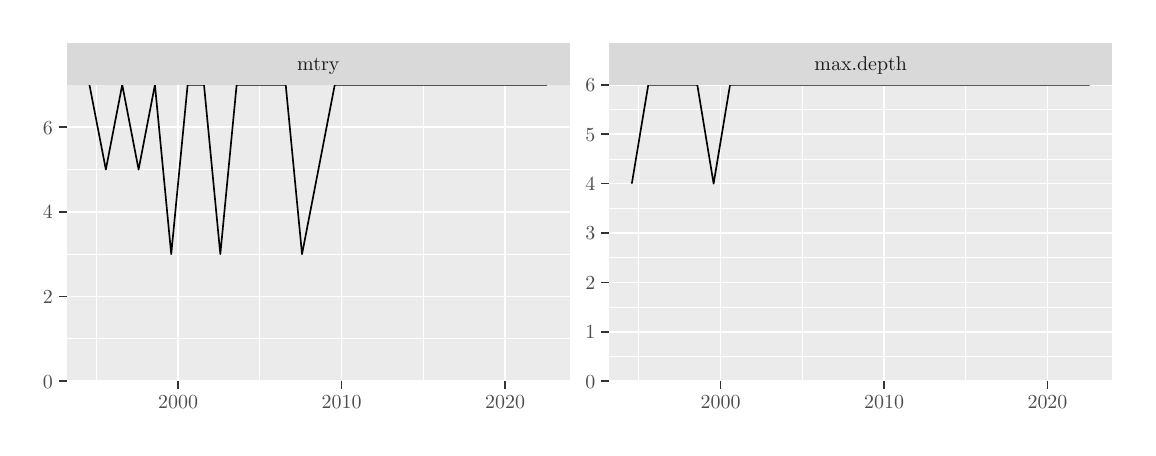
\begin{tikzpicture}[x=1pt,y=1pt]
\definecolor{fillColor}{RGB}{255,255,255}
\path[use as bounding box,fill=fillColor,fill opacity=0.00] (0,0) rectangle (397.48,144.54);
\begin{scope}
\path[clip] (  0.00,  0.00) rectangle (397.48,144.54);
\definecolor{drawColor}{RGB}{255,255,255}
\definecolor{fillColor}{RGB}{255,255,255}

\path[draw=drawColor,line width= 0.6pt,line join=round,line cap=round,fill=fillColor] (  0.00,  0.00) rectangle (397.48,144.54);
\end{scope}
\begin{scope}
\path[clip] ( 14.05, 16.81) rectangle (195.99,123.88);
\definecolor{fillColor}{gray}{0.92}

\path[fill=fillColor] ( 14.05, 16.81) rectangle (195.99,123.88);
\definecolor{drawColor}{RGB}{255,255,255}

\path[draw=drawColor,line width= 0.3pt,line join=round] ( 14.05, 32.10) --
	(195.99, 32.10);

\path[draw=drawColor,line width= 0.3pt,line join=round] ( 14.05, 62.70) --
	(195.99, 62.70);

\path[draw=drawColor,line width= 0.3pt,line join=round] ( 14.05, 93.29) --
	(195.99, 93.29);

\path[draw=drawColor,line width= 0.3pt,line join=round] ( 14.05,123.88) --
	(195.99,123.88);

\path[draw=drawColor,line width= 0.3pt,line join=round] ( 24.83, 16.81) --
	( 24.83,123.88);

\path[draw=drawColor,line width= 0.3pt,line join=round] ( 83.91, 16.81) --
	( 83.91,123.88);

\path[draw=drawColor,line width= 0.3pt,line join=round] (142.99, 16.81) --
	(142.99,123.88);

\path[draw=drawColor,line width= 0.6pt,line join=round] ( 14.05, 16.81) --
	(195.99, 16.81);

\path[draw=drawColor,line width= 0.6pt,line join=round] ( 14.05, 47.40) --
	(195.99, 47.40);

\path[draw=drawColor,line width= 0.6pt,line join=round] ( 14.05, 77.99) --
	(195.99, 77.99);

\path[draw=drawColor,line width= 0.6pt,line join=round] ( 14.05,108.59) --
	(195.99,108.59);

\path[draw=drawColor,line width= 0.6pt,line join=round] ( 54.37, 16.81) --
	( 54.37,123.88);

\path[draw=drawColor,line width= 0.6pt,line join=round] (113.46, 16.81) --
	(113.46,123.88);

\path[draw=drawColor,line width= 0.6pt,line join=round] (172.52, 16.81) --
	(172.52,123.88);
\definecolor{drawColor}{RGB}{0,0,0}

\path[draw=drawColor,line width= 0.6pt,line join=round] ( 22.32,123.88) --
	( 28.25, 93.29) --
	( 34.17,123.88) --
	( 40.08, 93.29) --
	( 45.98,123.88) --
	( 51.87, 62.70) --
	( 57.80,123.88) --
	( 63.71,123.88) --
	( 69.61, 62.70) --
	( 75.51,123.88) --
	( 81.42,123.88) --
	( 87.30,123.88) --
	( 93.24,123.88) --
	( 99.14, 62.70) --
	(105.06, 93.29) --
	(110.96,123.88) --
	(116.85,123.88) --
	(122.74,123.88) --
	(128.69,123.88) --
	(134.59,123.88) --
	(140.50,123.88) --
	(146.40,123.88) --
	(152.29,123.88) --
	(158.22,123.88) --
	(164.13,123.88) --
	(170.03,123.88) --
	(175.95,123.88) --
	(181.84,123.88) --
	(187.72,123.88);
\end{scope}
\begin{scope}
\path[clip] (210.04, 16.81) rectangle (391.98,123.88);
\definecolor{fillColor}{gray}{0.92}

\path[fill=fillColor] (210.04, 16.81) rectangle (391.98,123.88);
\definecolor{drawColor}{RGB}{255,255,255}

\path[draw=drawColor,line width= 0.3pt,line join=round] (210.04, 25.73) --
	(391.98, 25.73);

\path[draw=drawColor,line width= 0.3pt,line join=round] (210.04, 43.58) --
	(391.98, 43.58);

\path[draw=drawColor,line width= 0.3pt,line join=round] (210.04, 61.42) --
	(391.98, 61.42);

\path[draw=drawColor,line width= 0.3pt,line join=round] (210.04, 79.27) --
	(391.98, 79.27);

\path[draw=drawColor,line width= 0.3pt,line join=round] (210.04, 97.11) --
	(391.98, 97.11);

\path[draw=drawColor,line width= 0.3pt,line join=round] (210.04,114.96) --
	(391.98,114.96);

\path[draw=drawColor,line width= 0.3pt,line join=round] (220.83, 16.81) --
	(220.83,123.88);

\path[draw=drawColor,line width= 0.3pt,line join=round] (279.91, 16.81) --
	(279.91,123.88);

\path[draw=drawColor,line width= 0.3pt,line join=round] (338.98, 16.81) --
	(338.98,123.88);

\path[draw=drawColor,line width= 0.6pt,line join=round] (210.04, 16.81) --
	(391.98, 16.81);

\path[draw=drawColor,line width= 0.6pt,line join=round] (210.04, 34.65) --
	(391.98, 34.65);

\path[draw=drawColor,line width= 0.6pt,line join=round] (210.04, 52.50) --
	(391.98, 52.50);

\path[draw=drawColor,line width= 0.6pt,line join=round] (210.04, 70.34) --
	(391.98, 70.34);

\path[draw=drawColor,line width= 0.6pt,line join=round] (210.04, 88.19) --
	(391.98, 88.19);

\path[draw=drawColor,line width= 0.6pt,line join=round] (210.04,106.04) --
	(391.98,106.04);

\path[draw=drawColor,line width= 0.6pt,line join=round] (210.04,123.88) --
	(391.98,123.88);

\path[draw=drawColor,line width= 0.6pt,line join=round] (250.37, 16.81) --
	(250.37,123.88);

\path[draw=drawColor,line width= 0.6pt,line join=round] (309.45, 16.81) --
	(309.45,123.88);

\path[draw=drawColor,line width= 0.6pt,line join=round] (368.51, 16.81) --
	(368.51,123.88);
\definecolor{drawColor}{RGB}{0,0,0}

\path[draw=drawColor,line width= 0.6pt,line join=round] (218.31, 88.19) --
	(224.25,123.88) --
	(230.17,123.88) --
	(236.07,123.88) --
	(241.97,123.88) --
	(247.86, 88.19) --
	(253.80,123.88) --
	(259.70,123.88) --
	(265.60,123.88) --
	(271.51,123.88) --
	(277.41,123.88) --
	(283.30,123.88) --
	(289.23,123.88) --
	(295.13,123.88) --
	(301.05,123.88) --
	(306.96,123.88) --
	(312.84,123.88) --
	(318.73,123.88) --
	(324.68,123.88) --
	(330.59,123.88) --
	(336.49,123.88) --
	(342.39,123.88) --
	(348.28,123.88) --
	(354.21,123.88) --
	(360.12,123.88) --
	(366.02,123.88) --
	(371.94,123.88) --
	(377.83,123.88) --
	(383.71,123.88);
\end{scope}
\begin{scope}
\path[clip] ( 14.05,123.88) rectangle (195.99,139.04);
\definecolor{fillColor}{gray}{0.85}

\path[fill=fillColor] ( 14.05,123.88) rectangle (195.99,139.04);
\definecolor{drawColor}{gray}{0.10}

\node[text=drawColor,anchor=base,inner sep=0pt, outer sep=0pt, scale=  0.72] at (105.02,128.98) {mtry};
\end{scope}
\begin{scope}
\path[clip] (210.04,123.88) rectangle (391.98,139.04);
\definecolor{fillColor}{gray}{0.85}

\path[fill=fillColor] (210.04,123.88) rectangle (391.98,139.04);
\definecolor{drawColor}{gray}{0.10}

\node[text=drawColor,anchor=base,inner sep=0pt, outer sep=0pt, scale=  0.72] at (301.01,128.98) {max.depth};
\end{scope}
\begin{scope}
\path[clip] (  0.00,  0.00) rectangle (397.48,144.54);
\definecolor{drawColor}{gray}{0.20}

\path[draw=drawColor,line width= 0.6pt,line join=round] ( 54.37, 14.06) --
	( 54.37, 16.81);

\path[draw=drawColor,line width= 0.6pt,line join=round] (113.46, 14.06) --
	(113.46, 16.81);

\path[draw=drawColor,line width= 0.6pt,line join=round] (172.52, 14.06) --
	(172.52, 16.81);
\end{scope}
\begin{scope}
\path[clip] (  0.00,  0.00) rectangle (397.48,144.54);
\definecolor{drawColor}{gray}{0.30}

\node[text=drawColor,anchor=base,inner sep=0pt, outer sep=0pt, scale=  0.72] at ( 54.37,  6.90) {2000};

\node[text=drawColor,anchor=base,inner sep=0pt, outer sep=0pt, scale=  0.72] at (113.46,  6.90) {2010};

\node[text=drawColor,anchor=base,inner sep=0pt, outer sep=0pt, scale=  0.72] at (172.52,  6.90) {2020};
\end{scope}
\begin{scope}
\path[clip] (  0.00,  0.00) rectangle (397.48,144.54);
\definecolor{drawColor}{gray}{0.20}

\path[draw=drawColor,line width= 0.6pt,line join=round] (250.37, 14.06) --
	(250.37, 16.81);

\path[draw=drawColor,line width= 0.6pt,line join=round] (309.45, 14.06) --
	(309.45, 16.81);

\path[draw=drawColor,line width= 0.6pt,line join=round] (368.51, 14.06) --
	(368.51, 16.81);
\end{scope}
\begin{scope}
\path[clip] (  0.00,  0.00) rectangle (397.48,144.54);
\definecolor{drawColor}{gray}{0.30}

\node[text=drawColor,anchor=base,inner sep=0pt, outer sep=0pt, scale=  0.72] at (250.37,  6.90) {2000};

\node[text=drawColor,anchor=base,inner sep=0pt, outer sep=0pt, scale=  0.72] at (309.45,  6.90) {2010};

\node[text=drawColor,anchor=base,inner sep=0pt, outer sep=0pt, scale=  0.72] at (368.51,  6.90) {2020};
\end{scope}
\begin{scope}
\path[clip] (  0.00,  0.00) rectangle (397.48,144.54);
\definecolor{drawColor}{gray}{0.30}

\node[text=drawColor,anchor=base east,inner sep=0pt, outer sep=0pt, scale=  0.72] at (205.09, 14.33) {0};

\node[text=drawColor,anchor=base east,inner sep=0pt, outer sep=0pt, scale=  0.72] at (205.09, 32.17) {1};

\node[text=drawColor,anchor=base east,inner sep=0pt, outer sep=0pt, scale=  0.72] at (205.09, 50.02) {2};

\node[text=drawColor,anchor=base east,inner sep=0pt, outer sep=0pt, scale=  0.72] at (205.09, 67.87) {3};

\node[text=drawColor,anchor=base east,inner sep=0pt, outer sep=0pt, scale=  0.72] at (205.09, 85.71) {4};

\node[text=drawColor,anchor=base east,inner sep=0pt, outer sep=0pt, scale=  0.72] at (205.09,103.56) {5};

\node[text=drawColor,anchor=base east,inner sep=0pt, outer sep=0pt, scale=  0.72] at (205.09,121.40) {6};
\end{scope}
\begin{scope}
\path[clip] (  0.00,  0.00) rectangle (397.48,144.54);
\definecolor{drawColor}{gray}{0.20}

\path[draw=drawColor,line width= 0.6pt,line join=round] (207.29, 16.81) --
	(210.04, 16.81);

\path[draw=drawColor,line width= 0.6pt,line join=round] (207.29, 34.65) --
	(210.04, 34.65);

\path[draw=drawColor,line width= 0.6pt,line join=round] (207.29, 52.50) --
	(210.04, 52.50);

\path[draw=drawColor,line width= 0.6pt,line join=round] (207.29, 70.34) --
	(210.04, 70.34);

\path[draw=drawColor,line width= 0.6pt,line join=round] (207.29, 88.19) --
	(210.04, 88.19);

\path[draw=drawColor,line width= 0.6pt,line join=round] (207.29,106.04) --
	(210.04,106.04);

\path[draw=drawColor,line width= 0.6pt,line join=round] (207.29,123.88) --
	(210.04,123.88);
\end{scope}
\begin{scope}
\path[clip] (  0.00,  0.00) rectangle (397.48,144.54);
\definecolor{drawColor}{gray}{0.30}

\node[text=drawColor,anchor=base east,inner sep=0pt, outer sep=0pt, scale=  0.72] at (  9.10, 14.33) {0};

\node[text=drawColor,anchor=base east,inner sep=0pt, outer sep=0pt, scale=  0.72] at (  9.10, 44.92) {2};

\node[text=drawColor,anchor=base east,inner sep=0pt, outer sep=0pt, scale=  0.72] at (  9.10, 75.51) {4};

\node[text=drawColor,anchor=base east,inner sep=0pt, outer sep=0pt, scale=  0.72] at (  9.10,106.11) {6};
\end{scope}
\begin{scope}
\path[clip] (  0.00,  0.00) rectangle (397.48,144.54);
\definecolor{drawColor}{gray}{0.20}

\path[draw=drawColor,line width= 0.6pt,line join=round] ( 11.30, 16.81) --
	( 14.05, 16.81);

\path[draw=drawColor,line width= 0.6pt,line join=round] ( 11.30, 47.40) --
	( 14.05, 47.40);

\path[draw=drawColor,line width= 0.6pt,line join=round] ( 11.30, 77.99) --
	( 14.05, 77.99);

\path[draw=drawColor,line width= 0.6pt,line join=round] ( 11.30,108.59) --
	( 14.05,108.59);
\end{scope}
\end{tikzpicture}

\label{plot:RFHyperParams}
\end{figure}

\clearpage
\bibliographystyle{apacite}
\bibliography{References}

\end{document}